% !TEX program = xelatex
\documentclass[UTF8,fontset=fandol,a4paper,11pt]{ctexart}
\usepackage[margin=21mm,top=23mm,bottom=22mm,headheight=16pt]{geometry}
\usepackage{amsmath,amssymb,mathtools,bm}
\usepackage{tikz}
\usetikzlibrary{arrows.meta,calc,angles,quotes,patterns}
\usepackage{xcolor,booktabs,array,longtable,enumitem,fancyhdr,needspace}
\usepackage[unicode,hidelinks]{hyperref}
\definecolor{ink}{HTML}{24343C}
\definecolor{accent}{HTML}{166A70}
\definecolor{muted}{HTML}{65747A}
\definecolor{rulegray}{HTML}{D4DDE0}
\definecolor{warm}{HTML}{966037}
\color{ink}
\setlength{\parindent}{2em}
\setlength{\parskip}{4pt}
\linespread{1.12}
\AtBeginDocument{\setlength{\abovedisplayskip}{6pt plus 2pt minus 1pt}
\setlength{\belowdisplayskip}{6pt plus 2pt minus 1pt}
\setlength{\abovedisplayshortskip}{0pt plus 1pt}
\setlength{\belowdisplayshortskip}{4pt plus 1pt}}
\setlist[enumerate]{label=(\arabic*),leftmargin=2.3em,itemsep=3pt,topsep=4pt}
\setlist[itemize]{leftmargin=2em,itemsep=2pt,topsep=4pt}
\allowdisplaybreaks[1]
\setlength{\emergencystretch}{2em}
\setcounter{secnumdepth}{0}
\providecommand{\tightlist}{\setlength{\itemsep}{0pt}\setlength{\parskip}{0pt}}
\ctexset{section={format=\Large\bfseries\color{accent},beforeskip=10pt,afterskip=9pt},
subsection={format=\normalsize\bfseries\color{accent},beforeskip=10pt,afterskip=4pt},
subsubsection={format=\normalsize\bfseries,beforeskip=8pt,afterskip=3pt}}
\pagestyle{fancy}
\fancyhf{}
\fancyhead[L]{\small\color{muted}物理学难题集萃}
% 页眉仅保留书名；版本名称只在封面显示。
\fancyfoot[L]{\small\color{muted}\chapterlabel}
\fancyfoot[R]{\small\thepage}
\renewcommand{\headrulewidth}{0.4pt}
\renewcommand{\footrulewidth}{0pt}
\newcommand{\dd}{\mathop{}\!\mathrm{d}}
\newcommand{\vect}[1]{\bm{#1}}
\newcommand{\tagline}[1]{\noindent{\small\color{muted}#1}\par}
\newcommand{\result}[1]{\begin{equation*}\boxed{#1}\end{equation*}}
\newcommand{\figcaption}[1]{\par\vspace{2pt}{\small\color{muted}#1}\par}
\newcommand{\teach}[2]{\Needspace{4\baselineskip}\subsection*{讲解要点与追问}#1\par\smallskip\noindent\textbf{追问：}#2\par}
\newcommand{\workarea}{\par\vspace{7mm}\noindent{\small\color{muted}作答区}\par\vspace{4mm}
\noindent\textcolor{rulegray}{\rule{\linewidth}{0.3pt}}\par\vspace{16mm}
\noindent\textcolor{rulegray}{\rule{\linewidth}{0.3pt}}\par\vspace{16mm}
\noindent\textcolor{rulegray}{\rule{\linewidth}{0.3pt}}\par\vspace{16mm}
\noindent\textcolor{rulegray}{\rule{\linewidth}{0.3pt}}}
\tikzset{axis/.style={-{Stealth[length=2mm]},thin,color=muted},
motion/.style={-{Stealth[length=2.3mm]},thick,color=accent},
force/.style={-{Stealth[length=2.3mm]},thick,color=warm},
traj/.style={thick,color=accent},guide/.style={dashed,thin,color=muted},
object/.style={thick,color=ink},every node/.style={font=\small}}\widowpenalty=10000\clubpenalty=10000\displaywidowpenalty=10000\newcommand{\chapterlabel}{电磁学第二章\quad 磁场、磁介质}

\hypersetup{pdftitle={电磁学第二章 磁场、磁介质·教师版},pdfauthor={}}

\begin{document}

\pdfbookmark[0]{电磁学第二章 磁场、磁介质}{cover}

\thispagestyle{empty}\vspace*{22mm}
\noindent{\Huge\bfseries 物理学难题集萃}\par\vspace{10mm}
\noindent{\LARGE 电磁学第二章}\par\vspace{6mm}
\noindent{\LARGE 磁场、磁介质}\par\vspace{12mm}
\noindent{\Large\color{accent}教师版}\par\vspace{9mm}
\noindent\textcolor{accent}{\rule{\linewidth}{1pt}}\par\vspace{9mm}
\noindent 第1--27题\par\vfill\clearpage
\pdfbookmark[1]{题目目录}{contents}\section*{题目目录}
\begin{longtable}{@{}r p{113mm} r@{}}\toprule 题号 & 题目 & 页码\\\midrule

\hyperref[q:1]{1} & \hyperref[q:1]{半球面经线电流的球心磁场} & \pageref{q:1} \\

\hyperref[q:2]{2} & \hyperref[q:2]{抛物线形电流在焦点的磁场} & \pageref{q:2} \\

\hyperref[q:3]{3} & \hyperref[q:3]{均匀带电球面旋转的轴内磁场} & \pageref{q:3} \\

\hyperref[q:4]{4} & \hyperref[q:4]{无限长螺旋导线的轴上磁场} & \pageref{q:4} \\

\hyperref[q:5]{5} & \hyperref[q:5]{互补圆柱导体空隙中的均匀磁场} & \pageref{q:5} \\

\hyperref[q:6]{6} & \hyperref[q:6]{有限厚电流层的磁场分布} & \pageref{q:6} \\

\hyperref[q:7]{7} & \hyperref[q:7]{载流圆柱内的电子收缩与净电荷} & \pageref{q:7} \\

\hyperref[q:8]{8} & \hyperref[q:8]{磁场中转杆与滑动带电环} & \pageref{q:8} \\

\hyperref[q:9]{9} & \hyperref[q:9]{地磁场中带电圆环的滑动与纯滚动} & \pageref{q:9} \\

\hyperref[q:10]{10} & \hyperref[q:10]{电子枪击靶的圆轨道与螺旋轨道} & \pageref{q:10} \\

\hyperref[q:11]{11} & \hyperref[q:11]{平移细管内出射粒子追碰目标} & \pageref{q:11} \\

\hyperref[q:12]{12} & \hyperref[q:12]{方波轴向磁场中的电子束聚焦} & \pageref{q:12} \\

\hyperref[q:13]{13} & \hyperref[q:13]{同轴磁控管的临界磁场} & \pageref{q:13} \\

\hyperref[q:14]{14} & \hyperref[q:14]{点源到点像的磁场边界} & \pageref{q:14} \\

\hyperref[q:15]{15} & \hyperref[q:15]{电子束先会聚再扩束的四区磁场} & \pageref{q:15} \\

\hyperref[q:16]{16} & \hyperref[q:16]{环形磁场中的电子束聚焦与漂移} & \pageref{q:16} \\

\hyperref[q:17]{17} & \hyperref[q:17]{磁铁边缘场的单平面聚焦} & \pageref{q:17} \\

\hyperref[q:18]{18} & \hyperref[q:18]{电场漂移与磁场梯度漂移} & \pageref{q:18} \\

\hyperref[q:19]{19} & \hyperref[q:19]{重力与磁场中同高度的再相遇} & \pageref{q:19} \\

\hyperref[q:20]{20} & \hyperref[q:20]{载流双杆与弹簧的小振动} & \pageref{q:20} \\

\hyperref[q:21]{21} & \hyperref[q:21]{旋转带电圆环的附加张力} & \pageref{q:21} \\

\hyperref[q:22]{22} & \hyperref[q:22]{圆电流对共面长直导线的作用力} & \pageref{q:22} \\

\hyperref[q:23]{23} & \hyperref[q:23]{闭合稳恒电流回路间的作用与反作用} & \pageref{q:23} \\

\hyperref[q:24]{24} & \hyperref[q:24]{超导平板上方电流环的悬浮与振动} & \pageref{q:24} \\

\hyperref[q:25]{25} & \hyperref[q:25]{均匀磁化长棒侧面的场边界} & \pageref{q:25} \\

\hyperref[q:26]{26} & \hyperref[q:26]{均匀磁化球壳在球心的磁场} & \pageref{q:26} \\

\hyperref[q:27]{27} & \hyperref[q:27]{旋转径向极化圆柱的场能量} & \pageref{q:27} \\

\bottomrule\end{longtable}

\noindent 本章采用SI单位。$e>0$为电子电荷的绝对值，电子电荷为$-e$。图中$\odot$表示垂直纸面向外，$\otimes$表示垂直纸面向里；近似范围与其余符号在各题中说明。

\clearpage

\pdfbookmark[2]{第 1 题 半球面经线电流的球心磁场}{q1}

\section*{第 1 题\quad 半球面经线电流的球心磁场}\label{q:1}

半径为$R$的金属球面上，电流$2I$由南极流入、沿经线均匀分布后在北极流出，两端接沿极轴延伸的半无限长直导线。现沿过极轴的平面把球分成左右两半，移去右半球面；余下左半球面的电流分布保持不变，总电流为$I$。取极轴为$z$轴，左半球位于$y<0$，$x,y,z$构成右手坐标系。求球心$O$处的磁感应强度。

\begin{center}\begin{minipage}{.97\linewidth}\centering
\begin{tikzpicture}[x=1cm,y=1cm,font=\small]
\fill[accent!10] (0,-1.7) arc(-90:-270:1.7)--cycle;
\draw[object] (0,-1.7) arc(-90:-270:1.7);
\draw[guide] (0,-1.7)--(0,1.7);
\draw[axis] (0,0)--(2.7,0) node[right] {$y$};
\draw[axis] (0,0)--(0,2.85) node[above] {$z$};
\draw[motion] (0,-2.6)--(0,-1.75) node[midway,right] {$I$};
\draw[motion] (0,1.75)--(0,2.6) node[midway,right] {$I$};
\draw[motion] (-1.62,-.48) arc(-163:-197:1.7);
\node[left] at (-1.8,0) {$I:\ \mathrm S\to\mathrm N$};
\fill (0,0) circle(1.5pt) node[below right] {$O$};
\draw[<->] (0,0)--(-1.2,1.2) node[midway,above] {$R$};
\node at (1.8,-1.05) {$\odot\ +x$};
\node at (-.6,-2.95) {$yz$截面，保留$y<0$半球};
\end{tikzpicture}
\figcaption{图电2.1　过极轴的截面；箭头表示南极到北极的经线电流。切面为$y=0$，极轴两端接线均在球外。}
\end{minipage}\end{center}


\Needspace{8\baselineskip}

\pdfbookmark[3]{题型定位}{q1-h0}

\subsection*{题型定位}

把球面的稳恒电流按方位角分成经线半圆，再对半圆在球心的场作矢量积分。

\Needspace{8\baselineskip}

\pdfbookmark[3]{知识点}{q1-h1}

\subsection*{知识点}

半圆场为 $\mu_0\dd I/(4R)$。按等方位角分配电流给 $\dd I=I\dd\theta/\pi$。球面细带在极角 $\vartheta$ 处的宽度为 $R\sin\vartheta\dd\theta$；稳恒通过同一细带的电流固定，故 $K(\vartheta)\propto1/\sin\vartheta$。

\Needspace{8\baselineskip}

\pdfbookmark[3]{物理图像}{q1-h2}

\subsection*{物理图像}

解图电2.1A从 $-x$ 向 $-y$ 再到 $+x$ 量方位角。以中间经线为对称轴的两条场矢量给相同负 $x$ 分量，$y$ 分量反号。解图电2.1B给中间经线的叉乘方向，C图显示等角细带到了极区变窄、面电流密度变大。

\Needspace{8\baselineskip}

\pdfbookmark[3]{解题入口}{q1-h3}

\subsection*{解题入口}

先用毕奥—萨伐尔定律解释两段极轴接线的零叉乘。取一条从南极到北极的经线，求其半圆场的大小。再按解图电2.1A标出角度，把场写为 $(-\sin\theta,\cos\theta)$ 两分量后积分。

\Needspace{18\baselineskip}
\pdfbookmark[3]{标准解法}{q1-h4}

\subsection*{标准解法}

图电2.1中，接线在极轴上，任意接线元到$O$的位矢与电流元平行，所以$\dd\vect l\times\vect r=0$，接线不贡献球心磁场。把半球按经线方位角分成细条，每条从南极连到北极，都是半径$R$的半圆电流。

\begin{center}\begin{minipage}{.97\linewidth}\centering
\begin{tikzpicture}[x=1cm,y=1cm,font=\small]
\draw[axis] (-2.1,0)--(2.5,0) node[right] {$y$};
\draw[axis] (0,-2)--(0,2.1) node[above] {$x$};
\draw[object] (0,-1.6) arc(-90:-270:1.6);
\coordinate (O) at (0,0);
\fill (O) circle(1.4pt) node[above right] {$O$};
\coordinate (M) at (-1.131,-1.131);
\coordinate (N) at (-1.131,1.131);
\draw[guide] (O)--(M) node[below left] {$\theta$经线};
\draw[guide] (O)--(N) node[above left] {$\pi-\theta$经线};
\draw (0,-.48) arc(-90:-135:.48);
\node at (-.32,-.69) {$\theta$};
\draw[force] (O)--(.95,-.95) node[right] {$\mathrm d\boldsymbol B_\theta$};
\draw[force] (O)--(-.95,-.95) node[left] {$\mathrm d\boldsymbol B_{\pi-\theta}$};
\draw[motion] (O)--(0,-1.9) node[right] {合场沿$-x$};
\node[align=left] at (4.8,.8) {$\boldsymbol n=( -\cos\theta,-\sin\theta,0)$\\
$\mathrm d\boldsymbol B\parallel-\boldsymbol e_z\times\boldsymbol n$\\
$\mathrm d B_x=-\mathrm dB\sin\theta$\\
$\mathrm d B_y=\mathrm dB\cos\theta$};
\end{tikzpicture}
\figcaption{解图电2.1A　从$-x$向$-y$再到$+x$定义$0\le\theta\le\pi$。箭头都从O出发；配对后$y$分量抵消，$-x$分量相加。}
\end{minipage}\end{center}


解图电2.1A以$\theta\in[0,\pi]$标记经线平面，角度从$-x$端量起。原来全球总电流$2I$按$2\pi$方位均分，故细条中
\[
 \dd I=\frac{2I}{2\pi}\dd\theta=\frac I\pi\dd\theta.
\]
毕奥—萨伐尔定律给出半圆在圆心的磁场
\[
 \dd B=\frac{\mu_0\dd I}{4R}=\frac{\mu_0 I}{4\pi R}\dd\theta.
\]

在半球中间的经线取赤道附近的电流元来确定场方向：它沿$+z$，源点到$O$沿$+y$，故$\dd\vect l\times\vect r$沿$-x$。半圆上其余元的场同向，因此解图电2.1A的负$x$投影与真实电流方向一致。各细条电流满足$\int_0^\pi\dd I=I$，也与剩余半球的总量相符。

\Needspace{12\baselineskip}
按右手定则，各细条的场都在$xy$平面。关于半球中间经线对称的两条，$y$分量抵消，负$x$分量相加。按图的角度定义，$\dd B_x=-\dd B\sin\theta$，于是
\[
 B_x=-\frac{\mu_0 I}{4\pi R}\int_0^\pi\sin\theta\dd\theta
 =-\frac{\mu_0 I}{2\pi R},\qquad B_y=B_z=0.
\]
\result{\vect B(O)=-\frac{\mu_0 I}{2\pi R}\vect e_x.}
保留半球有向负 $x$ 的合场。完整球面上，跨过同一直径的两条经线赤道位置相反，半圆场也相反，逐对相加为零。

解图电2.1A把角度零点固定在赤道的$-x$端。若经线赤道位置的单位矢量为
\[
\boldsymbol n=-\cos\theta\,\boldsymbol e_x-\sin\theta\,\boldsymbol e_y,
\]
南极到北极的电流在该经线赤道处沿$+\boldsymbol e_z$，到O的位矢沿$-\boldsymbol n$，所以半圆场的单位方向为
\[
-\boldsymbol e_z\times\boldsymbol n
=-\sin\theta\,\boldsymbol e_x+\cos\theta\,\boldsymbol e_y.
\]
A图的两条场箭头按这两个分量同时绘制，角度零点和投影符号由此对应。
解图电2.1B选中间经线的真实电流元：向上的电流与向右的位矢叉乘，给出朝纸内的$-x$方向。

\begin{center}\begin{minipage}{.97\linewidth}\centering
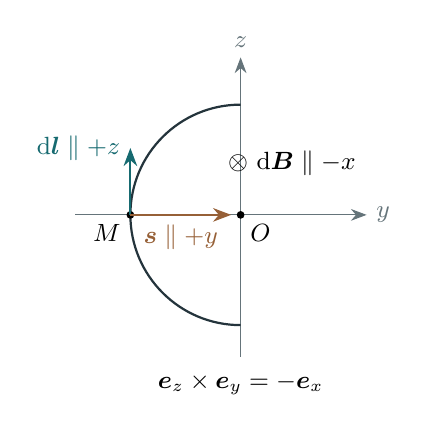
\begin{tikzpicture}[x=1cm,y=1cm,font=\small]
\draw[axis] (-2.1,0)--(1.6,0) node[right] {$y$};
\draw[axis] (0,-1.8)--(0,2) node[above] {$z$};
\draw[object] (0,-1.4) arc(-90:-270:1.4);
\fill (0,0) circle(1.4pt) node[below right] {$O$};
\fill (-1.4,0) circle(1.4pt) node[below left] {$M$};
\draw[motion] (-1.4,0)--(-1.4,.85) node[left] {$\mathrm d\boldsymbol l\parallel+z$};
\draw[force] (-1.4,0)--(-.12,0) node[midway,below] {$\boldsymbol s\parallel+y$};
\node at (.65,.65) {$\otimes\ \mathrm d\boldsymbol B\parallel-x$};
\node at (0,-2.15) {$\boldsymbol e_z\times\boldsymbol e_y=-\boldsymbol e_x$};
\end{tikzpicture}
\figcaption{解图电2.1B　取 $x=0,y=-R$ 处的电流元；图中 $+x$ 朝纸外，磁场朝纸内。}
\end{minipage}\end{center}

把角分配写成面电流密度，可以看清同一条细带怎样沿纬度传递电流。令$\vartheta$为从北极量起的极角，与方位角$\theta$不同。
在纬度$\vartheta$处，一条细带的横向宽度是$R\sin\vartheta\,\mathrm d\theta$；其面电流密度$K$满足
\[
\mathrm dI=K(\vartheta)R\sin\vartheta\,\mathrm d\theta
=\frac I\pi\,\mathrm d\theta,\qquad
K(\vartheta)=\frac{I}{\pi R\sin\vartheta}.
\]
\begin{center}\begin{minipage}{.97\linewidth}\centering
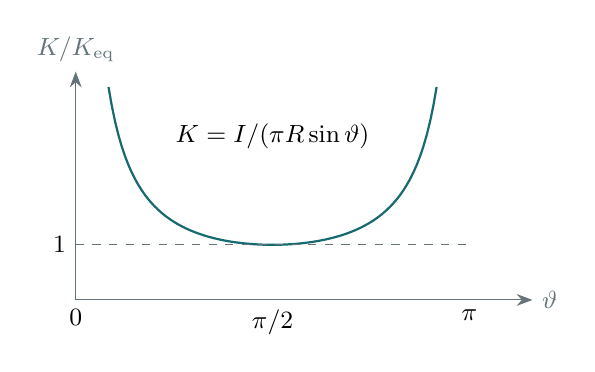
\begin{tikzpicture}[x=1cm,y=1cm,font=\small]
\draw[axis] (0,0)--(5.8,0) node[right] {$\vartheta$};
\draw[axis] (0,0)--(0,2.9) node[above] {$K/K_{\rm eq}$};
\draw[traj,domain=15:165,samples=100] plot ({5*\x/180},{.7/sin(\x)});
\draw[guide] (0,.7)--(5,.7);
\node[left] at (0,.7) {$1$};
\node[below] at (0,0) {$0$};\node[below] at (2.5,0) {$\pi/2$};\node[below] at (5,0) {$\pi$};
\node[above] at (2.5,1.8) {$K=I/(\pi R\sin\vartheta)$};
\end{tikzpicture}
\figcaption{解图电2.1C　经线面电流密度在两极附近增大；曲线只画远离极点的部分。每条细带的电流仍为$I\,\mathrm d\theta/\pi$。}
\end{minipage}\end{center}

解图电2.1C中的$K$并不处处相同；赤道值$K_{\rm eq}=I/(\pi R)$最小，两极的理想化发散来自电流汇入和流出同一点。
越靠近极点，细带宽度越小、面电流密度越大，两者相乘仍为同一细带电流。对任一纬圈在保留半球上的半周积分，
\[
\int_0^\pi K R\sin\vartheta\,\mathrm d\theta=I.
\]
稳恒条件固定的是穿过纬圈的总电流，因此面电流密度随纬圈半径按反比变化。


\Needspace{8\baselineskip}

\pdfbookmark[3]{关键洞察}{q1-h5}

\subsection*{关键洞察}

等角电流密度给每条细带相同权重，几何投影再乘 $\sin\theta$ 或 $\cos\theta$。切口附近的细带负 $x$ 投影较小，中部经线负 $x$ 投影最大。恢复右半球时，两半球的中心场大小相等、方向相反。

\Needspace{8\baselineskip}

\pdfbookmark[3]{易错点}{q1-h6}

\subsection*{易错点}

\begin{itemize}
\item 全球总电流 $2I$ 平均在 $2\pi$ 角域，剩余 $\pi$ 角域内总量为 $I$。
\item 每条经线的场方向随 $\theta$ 转动；沿负 $x$ 方向的分量参与相加。
\item 极轴导线位于球外，线元与指向球心的位矢平行。
\item 改半径时先分清固定的是总电流还是面电流密度。
\end{itemize}

\Needspace{8\baselineskip}

\pdfbookmark[3]{课堂讲解建议}{q1-h7}

\subsection*{课堂讲解建议}

在解图电2.1B先用一根手指指向电流、另一根沿源点到球心的方向，确定中间经线的场为负 $x$。回到解图电2.1A任选两条对称经线，分别写两场分量，再让学生指出为什么 $y$ 项相反、负 $x$ 项相同。

积分前把 $I/\pi$、半圆因子 $1/(4R)$ 和投影 $\sin\theta$ 各写一行，追问它们来自哪个图中对象。变图电2.1V7改为固定赤道面电流密度，先读赤道带宽怎样改变，再求总电流和场。

\Needspace{18\baselineskip}
\pdfbookmark[3]{变式训练}{q1-h8}

\subsection*{变式训练}

\begin{enumerate}
\item 恢复全球，保持每单位方位角电流为 $I/\pi$。右半球由左半球绕 $z$ 轴转 $\pi$ 得到，电流方向随几何一起转动。变图电2.1V1的两个中心场因此为 $-\mu_0 I\vect e_x/(2\pi R)$ 和 $+\mu_0 I\vect e_x/(2\pi R)$，相加为零。此时全球总电流为 $2I$；若改成全球总电流 $I$，两个贡献各减半，仍然相消。
\begin{center}\begin{minipage}{.98\linewidth}\centering
\begin{tikzpicture}[scale=.85,transform shape]
\draw[axis](-2.8,0)--(2.9,0)node[right]{$x$};\draw[axis](0,-2.3)--(0,2.48)node[above]{$y$};
\draw[object](0,0)circle(1.55);
\draw[motion](-.13,.28)--(-2.39,.28)node[above left]{$\vect B_{\text{左}}$};
\draw[motion](.13,-.28)--(2.39,-.28)node[below right]{$\vect B_{\text{右}}$};
\node at(-1.0,-1.83){$y<0$};
\node at(1.0,1.86){$y>0$};
\end{tikzpicture}
\figcaption{变图电2.1V1\quad 完整球面两半的中心场大小相等、方向相反}
\end{minipage}\end{center}
\item 把保留半球的总电流改成 $J$，经线仍在 $[0,\pi]$ 内均分，故 $\dd I=(J/\pi)\dd\theta$。将半圆场乘投影并积分，
\[
B_x=-\frac{\mu_0 J}{4\pi R}\int_0^\pi\sin\theta\dd\theta=-\frac{\mu_0 J}{2\pi R},
\qquad B_y=0.
\]
变图电2.1V2的直线按参考电流 $I$ 归一化，展示了场大小随总电流同比变化。
\begin{center}\begin{minipage}{.98\linewidth}\centering
\begin{tikzpicture}[scale=.85,transform shape]
\draw[axis](0,0)--(5.7,0)node[right]{$J/I$};
\draw[axis](0,0)--(0,3.45)node[above]{$|B_x|/|B_x(I)|$};
\draw[traj](0,0)--(5.15,2.96);
\draw[guide](2.2,0)--(2.2,1.264);
\fill(2.2,1.264)circle(1.5pt)node[above left]{$(1,1)$};
\node[below]at(2.2,0){$1$};
\end{tikzpicture}
\figcaption{变图电2.1V2\quad 角分布形状固定时，半球场与总电流成正比}
\end{minipage}\end{center}
\item 只保留 $\theta_1\le\theta\le\theta_2$ 的经线，沿用 $\dd I=I\dd\theta/\pi$。由变图电2.1V3的两轴读分量，令 $K=\mu_0I/(4\pi R)$，则
\[
B_x=-K\int_{\theta_1}^{\theta_2}\sin\theta\dd\theta
=-K(\cos\theta_1-\cos\theta_2),\quad
B_y=K(\sin\theta_2-\sin\theta_1).
\]
图示 $\theta_1=\pi/6,\theta_2=\pi/2$，给 $(-\sqrt3 K/2,K/2)$。对非空角域，$y$ 项为零时两端的正弦相等，角域关于 $\pi/2$ 对称。
\begin{center}\begin{minipage}{.98\linewidth}\centering
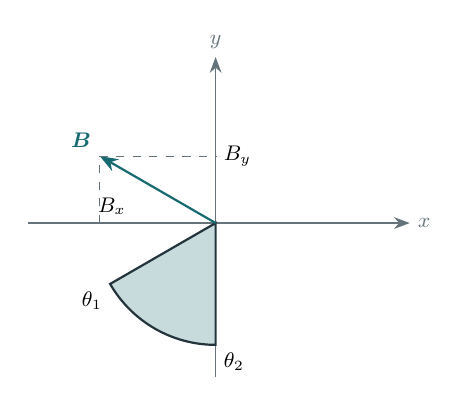
\begin{tikzpicture}[scale=.85,transform shape]
\draw[axis](-2.8,0)--(2.9,0)node[right]{$x$};\draw[axis](0,-2.3)--(0,2.48)node[above]{$y$};
\fill[accent!24](0,0)--(210:1.82)arc(210:270:1.82)--cycle;
\draw[object](0,0)--(210:1.82)arc(210:270:1.82)--cycle;
\node[below left]at(210:1.82){$\theta_1$};
\node[below right]at(270:1.82){$\theta_2$};
\draw[motion](0,0)--(-1.73,1.00)node[above left]{$\vect B$};
\draw[guide](-1.73,0)--(-1.73,1)--(0,1);
\node[above left]at(-1.22,0){$B_x$};
\node[right]at(0,1){$B_y$};
\end{tikzpicture}
\figcaption{变图电2.1V3\quad 赤道面所保留的角域偏向一侧，合场有两个分量}
\end{minipage}\end{center}
\item 半径加倍、半球总电流和归一化角分布保持。变图电2.1V4中，同一经线对应的新半圆半径为 $2R$，其 $\dd B$ 由 $\mu_0\dd I/(4R)$ 降为 $\mu_0\dd I/(8R)$。积分角域和各方向投影保持，所以合场减半。面电流密度固定时，应先由新带宽求出 $\dd I$，如变图电2.1V7。
\begin{center}\begin{minipage}{.98\linewidth}\centering
\begin{tikzpicture}[scale=.85,transform shape]
\draw[object](0,0)arc(180:0:1.75);
\draw[traj](.875,0)arc(180:0:.875);
\fill(1.75,0)circle(1.5pt)node[below]{$O$};
\draw[<->](1.75,.22)--(2.625,.22)node[midway,above]{$R$};
\draw[<->](0,-.55)--(1.75,-.55)node[midway,below]{$2R$};
\node[right]at(3.72,1.28){$\dd I$ 保持};
\end{tikzpicture}
\figcaption{变图电2.1V4\quad 各经线半径加倍，细带电流保持，场的尺度减半}
\end{minipage}\end{center}
\item 方位电流取 $\dd I=w(\theta)\dd\theta$，则
\[
B_x=-\frac{\mu_0}{4R}\int_0^\pi w\sin\theta\,\dd\theta,\qquad
B_y=\frac{\mu_0}{4R}\int_0^\pi w\cos\theta\,\dd\theta.
\]
变图电2.1V5比较均匀分布和 $w=(I/\pi)(1+0.6\cos2\theta)$。两曲线积分同为 $I$，且都对称，故 $B_y=0$。后者将电流偏向两切口，$\int_0^\pi\sin\theta\cos2\theta\,\dd\theta=-2/3$，所以负 $x$ 分量大小为均匀值的 $1-0.6/3=0.8$ 倍。总电流相同的情况下，两项角投影仍由具体分布决定。
\begin{center}\begin{minipage}{.98\linewidth}\centering
\begin{tikzpicture}[scale=.85,transform shape]
\draw[axis](0,0)--(6.1,0)node[right]{$\theta$};
\draw[axis](0,0)--(0,3.35)node[above]{$w/(I/\pi)$};
\begin{scope}[x=.029cm,y=1.65cm]
\draw[object,dashed](0,1)--(180,1);
\draw[traj,domain=0:180,samples=90]plot(\x,{1+.6*cos(2*\x)});
\node[below]at(90,0){$\pi/2$};
\node[below]at(180,0){$\pi$};
\end{scope}
\node[above]at(1.15,2.68){偏向切口};
\node[above]at(3.02,1.65){均匀};
\end{tikzpicture}
\figcaption{变图电2.1V5\quad 两种分布总电流相同，负 $x$ 分量的投影积分不同}
\end{minipage}\end{center}
\item 令 $w=(I/\pi)(1+\eta\cos\theta)$，$|\eta|\le1$。余弦项对总电流和 $B_x$ 的积分都为零；对 $B_y$ 则留下 $\eta\int_0^\pi\cos^2\theta\dd\theta=\eta\pi/2$。所以 $B_x=-\mu_0I/(2\pi R),\,B_y=\mu_0I\eta/(8R)$。变图电2.1V6取 $\eta>0$，合场从负 $x$ 朝正 $y$ 偏，偏角正切为 $\pi\eta/4$；$\eta<0$ 时偏向下方。
\begin{center}\begin{minipage}{.98\linewidth}\centering
\begin{tikzpicture}[scale=.85,transform shape]
\draw[axis](-2.8,0)--(2.9,0)node[right]{$x$};\draw[axis](0,-2.3)--(0,2.48)node[above]{$y$};
\draw[motion](0,0)--(-2.18,0)node[midway,below]{$B_x$};
\draw[motion](-2.18,0)--(-2.18,1.37)node[midway,left]{$B_y$};
\draw[motion](0,0)--(-2.18,1.37)node[above left]{$\vect B$};
\draw[guide](-2.18,1.37)--(0,1.37);
\node[right]at(.2,1.17){$\eta>0$};
\end{tikzpicture}
\figcaption{变图电2.1V6\quad 偏向小方位角的电流增加时，出现正 $y$ 场分量}
\end{minipage}\end{center}
\item 固定赤道面电流密度 $K_{\rm eq}$。赤道处保留半周的有效宽度为 $\pi R$，电流沿经线垂直穿过赤道，故 $I=\pi RK_{\rm eq}$。变图电2.1V7半径变为 $2R$ 时，两倍宽度给两倍总电流，$I/R$ 保持，所以 $B_x=-\mu_0K_{\rm eq}/2$ 保持。
\begin{center}\begin{minipage}{.98\linewidth}\centering
\begin{tikzpicture}[scale=.85,transform shape]
\node[draw,align=center](a)at(.65,1.1){$R$\\$I=\pi R K_{\rm eq}$};
\node[draw,align=center](b)at(5.35,1.1){$2R$\\$I'=2\pi RK_{\rm eq}$};
\draw[motion](a.east)--(b.west)node[midway,above]{$K_{\rm eq}$ 固定};
\node[below]at(3,.14){$I'/R'=I/R$};
\end{tikzpicture}
\figcaption{变图电2.1V7\quad 固定赤道电流密度时，半径加倍使总量也加倍}
\end{minipage}\end{center}
\item 若改动接线，按其实际路径算毕奥—萨伐尔积分。变图电2.1V8示例另有一条平行 $z$ 轴、位于 $x=b$ 的无限长直导线，电流沿 $+z$，其在 O 的场为 $-\mu_0 I\vect e_y/(2\pi b)$，因为从导线指向 O 的横向位移沿 $-x$。再加球面场 $-\mu_0 I\vect e_x/(2\pi R)$，得到两分量。两段原轴线接线由于每个源点的位矢与线元平行，仍给零贡献。
\begin{center}\begin{minipage}{.98\linewidth}\centering
\begin{tikzpicture}[scale=.85,transform shape]
\draw[axis](-2.8,0)--(2.9,0)node[right]{$x$};\draw[axis](0,-2.3)--(0,2.48)node[above]{$y$};
\fill(0,0)circle(1.4pt)node[above left]{$O$};
\draw[object](1.94,0)circle(6pt);\fill(1.94,0)circle(1.4pt);
\node[above]at(1.94,.23){导线 $I$ 朝纸外};
\draw[<->](0,-.31)--(1.94,-.31)node[midway,below]{$b$};
\draw[motion](0,0)--(-1.9,0)node[midway,above]{$\vect B_{\text{球}}$};
\draw[motion](0,0)--(0,-1.7)node[below]{$\vect B_{\text{线}}$};
\draw[motion](0,0)--(-1.9,-1.7)node[left]{$\vect B$};
\end{tikzpicture}
\figcaption{变图电2.1V8\quad 偏轴补充直导线的磁场按右手定则取向，再与球面场相加}
\end{minipage}\end{center}
\end{enumerate}

\clearpage

\pdfbookmark[2]{第 2 题 抛物线形电流在焦点的磁场}{q2}

\section*{第 2 题\quad 抛物线形电流在焦点的磁场}\label{q:2}

一根无限长细导线弯成抛物线，焦点到顶点的距离为$a$，通有恒定电流$I$。取抛物线为$x^2=4ay$，焦点$P=(0,a)$，电流从左支流向顶点，再沿右支流出。求$P$处的磁感应强度。

\begin{center}\begin{minipage}{.98\linewidth}\centering
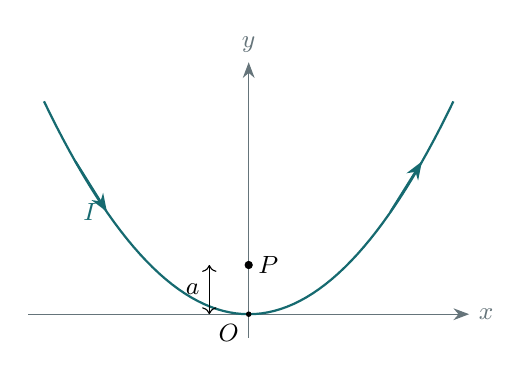
\begin{tikzpicture}[x=1cm,y=1cm]
\draw[axis] (-2.8,0)--(2.8,0) node[right] {$x$};\draw[axis] (0,-.3)--(0,3.2) node[above] {$y$};\draw[traj,domain=-2.6:2.6,samples=65] plot(\x,{.4*\x*\x});
\fill (0,0) circle(1pt) node[below left] {$O$};\fill (0,.625) circle(1.5pt) node[right] {$P$};\draw[<->] (-.5,0)--(-.5,.625) node[midway,left] {$a$};\draw[motion] (-2.2,1.94)--(-1.8,1.3) node[left] {$I$};\draw[motion] (1.8,1.3)--(2.2,1.94);
\end{tikzpicture}\figcaption{图电2.2　电流沿左支向下、右支向上。}\end{minipage}\end{center}

\Needspace{8\baselineskip}

\pdfbookmark[3]{题型定位}{q2-h0}

\subsection*{题型定位}

将焦点几何与平面曲线的毕奥—萨伐尔积分结合，求非圆导线的磁场。

\Needspace{8\baselineskip}

\pdfbookmark[3]{知识点}{q2-h1}

\subsection*{知识点}

毕奥—萨伐尔核由电流元到场点的位矢和叉乘组成。对 $y=x^2/(4a)$，$xy^\prime=2y$，焦点距离 $s=a+y$，两者使磁场分子和距离共享一个因子。

\Needspace{8\baselineskip}

\pdfbookmark[3]{物理图像}{q2-h2}

\subsection*{物理图像}

解图电2.2A在右支取沿右上的电流元，到焦点的箭头指向左下。左支电流向右下，位置向量也改变，两个 $z$ 分量仍同向。解图电2.2B用等距的焦点、准线说明 $s=a+y$，C图用核的面积读各段的贡献。

\Needspace{8\baselineskip}

\pdfbookmark[3]{解题入口}{q2-h3}

\subsection*{解题入口}

先写 $\dd\vect l=(1,y^\prime,0)\dd x$，把源点指向 P 的位矢写成 $(-x,a-y,0)$。用抛物线方程简化叉乘和距离，再令 $x/(2a)=\tan\alpha$ 积分。核按 $x^{-4}$ 衰减，远处尾部积分有限。

\Needspace{18\baselineskip}
\pdfbookmark[3]{标准解法}{q2-h4}

\subsection*{标准解法}

解图电2.2A在右支取电流元，按电流方向以$x$为参数，$x$从$-\infty$增至$+\infty$。电流元位置$(x,y)$，到焦点的位矢为
\[
 \vect s=-x\vect e_x+(a-y)\vect e_y,\qquad
 \dd\vect l=\dd x\vect e_x+\dd y\vect e_y.
\]
\begin{center}\begin{minipage}{.98\linewidth}\centering
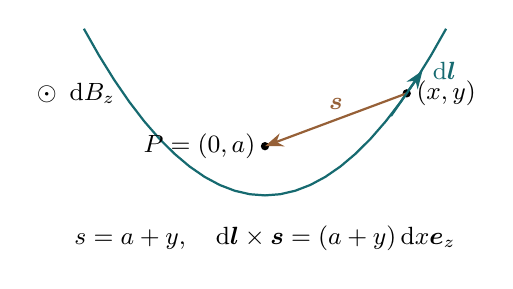
\begin{tikzpicture}[x=1cm,y=1cm]
\draw[traj,domain=-2.3:2.3] plot(\x,{.4*\x*\x});\fill (0,.625) circle(1.5pt) node[left] {$P=(0,a)$};\fill (1.8,1.296) circle(1.5pt) node[right] {$(x,y)$};\draw[force] (1.8,1.296)--(0,.625) node[midway,above] {$\vect s$};\draw[motion] (1.6,1.008)--(2,1.584) node[right] {$\dd\vect l$};\node at (-2.4,1.3) {$\odot\ \dd B_z$};\node at (0,-.55) {$s=a+y,\quad \dd\vect l\times\vect s=(a+y)\dd x\vect e_z$};
\end{tikzpicture}\figcaption{解图电2.2A　电流元到焦点的距离和叉乘均可用a+y表示。}\end{minipage}\end{center}
由$y=x^2/(4a)$，有$y'=x/(2a)$，因而
\[
 \dd\vect l\times\vect s
 =[a-y+xy']\dd x\vect e_z=(a+y)\dd x\vect e_z.
\]
这里$\vect e_z$垂直纸面向外。抛物线的焦点距离满足
\[
 s^2=x^2+(a-y)^2=4ay+(a-y)^2=(a+y)^2,
 \qquad s=a+y>0.
\]
所以所有电流元的磁场均沿正$z$方向，且
\[
 \dd B_z=\frac{\mu_0 I}{4\pi}\frac{(a+y)\dd x}{s^3}
 =\frac{\mu_0 I}{4\pi a^2}\frac{\dd x}{[1+(x/2a)^2]^2}.
\]
左右两支的被积函数相同。令$x=2a\tan\alpha$，$\dd x=2a\sec^2\alpha\dd\alpha$，则
\[
 B_z=\frac{\mu_0 I}{2\pi a^2}\int_0^\infty\frac{\dd x}{[1+(x/2a)^2]^2}
 =\frac{\mu_0 I}{\pi a}\int_0^{\pi/2}\cos^2\alpha\dd\alpha
 =\frac{\mu_0 I}{4a}.
\]

\Needspace{14\baselineskip}
以切线倾角 $\alpha$ 为变量，正半支的 $x:0\to\infty$ 对应 $\alpha:0\to\pi/2$，并有
\[\frac{\dd x}{[1+(x/2a)^2]^2}
=\frac{2a\sec^2\alpha\dd\alpha}{\sec^4\alpha}
=2a\cos^2\alpha\dd\alpha.\]
解图电2.2A中每个电流元的叉乘分子为 $a+y>0$。左右两支上的电流都沿 $x$ 增加的方向，且互为镜像的两点有相同 $y$，所以给相等、同向的磁场微元。

这里的最后一个积分可直接展开：
\[
 \int_0^{\pi/2}\cos^2\alpha\,\dd\alpha
 =\left[\frac{\alpha}{2}+\frac{\sin2\alpha}{4}\right]_0^{\pi/2}
 =\frac{\pi}{4}.
\]
全轴积分化成两倍正半轴积分的因子已经计在前面的系数中。

\result{\vect B(P)=\frac{\mu_0 I}{4a}\vect e_z.}
反向通电时方向反转；整个计算中的$a$是焦距，若使用方程$x^2=2py$，应先代入$p=2a$。

解图电2.2B给出$s=a+y$的几何解释：焦点到曲线上 M 的距离，等于 M 到准线 $y=-a$ 的距离。
焦点与准线是这一定义中的配对对象。若改用场点 $(0,2a)$，其距离应写成 $\sqrt{x^2+(2a-y)^2}$，按新核积分。
同时，切线斜率$y'=x/(2a)$给$\tan\alpha=x/(2a)$，所以积分中的三角换元正好使用切线倾角。
图中示例$x=2a$给$\alpha=\pi/4$、$y=a$、$s=2a$，此时到焦点的距离与到水平准线的距离都为 $2a$。
\begin{center}\begin{minipage}{.97\linewidth}\centering
\begin{tikzpicture}[x=1.6cm,y=1.6cm,font=\small]
\draw[axis] (-1.8,0)--(2.7,0) node[right] {$x$};
\draw[axis] (0,-.95)--(0,2) node[above] {$y$};
\draw[traj,domain=-1.7:1.7,samples=70] plot(\x,{.4*\x*\x});
\draw[guide] (-1.8,-.625)--(2.5,-.625) node[right] {准线$y=-a$};
\coordinate (M) at (1.25,.625);\coordinate (P) at (0,.625);\coordinate (N) at (1.25,-.625);
\fill (P) circle(1.4pt) node[left] {$P$};
\fill (M) circle(1.4pt) node[below right] {$M$};
\draw[force] (M)--(P) node[midway,above=6pt] {$s=a+y$};
\draw[guide] (M)--(N) node[pos=.72,right] {$a+y$};
\draw[object] (1.25,-.49)--(1.12,-.49)--(1.12,-.625);
\draw[motion] (M)--(1.85,1.225) node[above] {切线};
\draw[guide] (M)--(2.05,.625);
\draw (1.6,.625) arc(0:45:.35);
\node at (1.83,.84) {$\alpha$};
\node[below right] at (0,0) {$O$};
\node[below] at (1.25,-.625) {$N$};
\end{tikzpicture}
\figcaption{解图电2.2B　示例取$x=2a$；焦点距离MP等于到准线的距离MN。切线倾角满足$\tan\alpha=x/(2a)$。}
\end{minipage}\end{center}

解图电2.2C显示每一段对全积分的贡献。只计算$|x|\le X$的导线段，令$u=X/(2a)\ge0$，则
\[
G(u)=\arctan u+\frac{u}{1+u^2},\qquad
B(X)=\frac{\mu_0I}{2\pi a}G(u).
\]
这是该段的场；连接两端所需导线的贡献须按其实际位置另计，或明确使其远离焦点。
\begin{center}\begin{minipage}{.97\linewidth}\centering
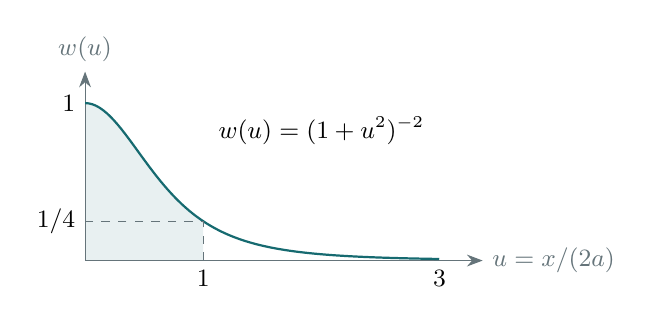
\begin{tikzpicture}[x=1cm,y=1cm,font=\small]
\fill[accent!10] (0,0)--plot[domain=0:1,samples=50] ({1.5*\x},{2/(1+\x*\x)^2})--(1.5,0)--cycle;
\draw[axis] (0,0)--(5.05,0) node[right] {$u=x/(2a)$};
\draw[axis] (0,0)--(0,2.4) node[above] {$w(u)$};
\draw[traj,domain=0:3,samples=100] plot({1.5*\x},{2/(1+\x*\x)^2});
\draw[guide] (1.5,0)--(1.5,.5)--(0,.5);
\node[left] at (0,2) {$1$};\node[left] at (0,.5) {$1/4$};
\node[below] at (1.5,0) {$1$};\node[below] at (4.5,0) {$3$};
\node[above] at (3,1.35) {$w(u)=(1+u^2)^{-2}$};
\end{tikzpicture}
\figcaption{解图电2.2C　正半支的真实无量纲积分核。阴影对应$0\le x\le2a$；两支按同一范围截取后，磁场占全导线约81.8\%。}
\end{minipage}\end{center}

由解图电2.2C的面积，保留中央$|x|\le2a$时，
\[
\frac{B(2a)}{B(\infty)}
=\frac2\pi\left(\frac\pi4+\frac12\right)
=\frac12+\frac1\pi\simeq0.8183.
\]
远处的核按 $u^{-4}$ 下降，沿尾部积分后得到三次倒数的首项：
\[
1-\frac{B(X)}{B(\infty)}
=\frac4{3\pi u^3}+O(u^{-5}),\qquad u\gg1.
\]
C图中的核处处为正；各段的场都沿$+z$，截短只减小大小，方向保持不变。

\Needspace{8\baselineskip}

\pdfbookmark[3]{关键洞察}{q2-h5}

\subsection*{关键洞察}

同一个 $a+y$ 同时出现在焦点距离和叉乘中，所以被积核降为距离的平方倒数。三角换元中的角正是切线倾角。若更换场点，位矢和距离先按新的场点重写。

\Needspace{8\baselineskip}

\pdfbookmark[3]{易错点}{q2-h6}

\subsection*{易错点}

\begin{itemize}
\item $x$ 沿电流从负无穷增至正无穷，左右两支同向贡献。
\item 电流元的 $\dd y$ 分量给叉乘中的 $xy^\prime$。
\item 方程 $x^2=2py$ 的焦距是 $p/2$。
\item 化为两倍正半轴积分的因子2与换元微分中的 $2a$ 分别来自对称性与坐标尺度。
\end{itemize}

\Needspace{8\baselineskip}

\pdfbookmark[3]{课堂讲解建议}{q2-h7}

\subsection*{课堂讲解建议}

在解图电2.2A画出相同高度的左右电流元，分别写两个叉乘的 $z$ 分量。让学生从 $xy^\prime=2y$ 得到同一个正分子，再借B图说明分母的距离为什么也等于 $a+y$。

在C图上遮住两条尾部，让学生从核的正性判断截断后是偏大还是偏小。用变图电2.2V7比较渐近值与实际尾积分，再算给定误差所需的截段长度。

\Needspace{18\baselineskip}
\pdfbookmark[3]{变式训练}{q2-h8}

\subsection*{变式训练}

\begin{enumerate}
\item 将导线上的电流反向。变图电2.2V1中从电流元指向 P 的 $\vect s$ 仍沿虚线，电流元矢量改向，故 $\dd\vect l\times\vect s$ 反号。积分距离因子保持，于是 $\vect B=-\mu_0 I\vect e_z/(4a)$，指向纸内。
\begin{center}\begin{minipage}{.98\linewidth}\centering
\begin{tikzpicture}[scale=.85,transform shape]
\draw[traj,domain=-2.45:2.45,samples=64]plot(\x,{.32*(\x)^2});
\fill(0,.78125)circle(1.4pt)node[above left]{$P$};
\draw[guide](1.82,1.06)--(0,.78125)node[midway,below]{$\vect s$};

\draw[motion](1.86,1.107)--(1.25,.50)node[midway,right]{反向电流};
\node[left]at(-1.7,1.49){$\otimes\ B_z$};
\end{tikzpicture}
\figcaption{变图电2.2V1\quad 反向通电后，位置向量保持，叉乘及磁场反向}
\end{minipage}\end{center}
\item 把方程写成 $x^2=2py$。变图电2.2V2中，焦点到顶点的距离 $a$ 由 $4a=2p$ 得 $p/2$。代入 $\mu_0 I/(4a)$，有 $B=\mu_0 I/(2p)$；电流仍由左向右时方向为纸外。
\begin{center}\begin{minipage}{.98\linewidth}\centering
\begin{tikzpicture}[scale=.85,transform shape]
\draw[axis](-2.8,0)--(2.95,0)node[right]{$x$};
\draw[axis](0,-1.33)--(0,2.9)node[above]{$y$};
\draw[traj,domain=-2.45:2.45,samples=72]plot(\x,{(\x)^2/4});
\draw[guide](-2.45,-1)--(2.45,-1)node[right]{准线};
\fill(0,1)circle(1.4pt)node[above left]{$P$};
\fill(0,0)circle(1.4pt)node[below left]{$O$};
\draw[<->](.26,0)--(.26,1)node[midway,right]{$p/2$};
\end{tikzpicture}
\figcaption{变图电2.2V2\quad 将方程写成 $x^2=2py$ 时，顶点到焦点的距离为 $p/2$}
\end{minipage}\end{center}
\item 截取 $|x|\le X$，回线若离焦点足够远，则本段给主要贡献。用 $u=X/(2a)$，因核偶对称，变图电2.2V3的两半阴影面积相等。由
\[
\int\frac{\dd u}{(1+u^2)^2}
=\frac12\left(\arctan u+\frac{u}{1+u^2}\right)
\]
得该段 $B_z=\mu_0 I[\arctan u+u/(1+u^2)]/(2\pi a)$。有限距离的连接导线另按其实际路径作矢量积分。
\begin{center}\begin{minipage}{.98\linewidth}\centering
\begin{tikzpicture}[scale=.85,transform shape]
\draw[axis](-4.05,0)--(4.32,0)node[right]{$u$};\draw[axis](0,0)--(0,3.05)node[above]{$(1+u^2)^{-2}$};\fill[accent!23](-1.42000,0)--(-1.42000,0.63750)--(-1.37761,0.67671)--(-1.33522,0.71830)--(-1.29284,0.76235)--(-1.25045,0.80895)--(-1.20806,0.85819)--(-1.16567,0.91012)--(-1.12328,0.96479)--(-1.08090,1.02223)--(-1.03851,1.08243)--(-0.99612,1.14538)--(-0.95373,1.21100)--(-0.91134,1.27919)--(-0.86896,1.34980)--(-0.82657,1.42263)--(-0.78418,1.49741)--(-0.74179,1.57383)--(-0.69940,1.65151)--(-0.65701,1.73000)--(-0.61463,1.80878)--(-0.57224,1.88726)--(-0.52985,1.96480)--(-0.48746,2.04069)--(-0.44507,2.11420)--(-0.40269,2.18452)--(-0.36030,2.25085)--(-0.31791,2.31239)--(-0.27552,2.36832)--(-0.23313,2.41790)--(-0.19075,2.46041)--(-0.14836,2.49523)--(-0.10597,2.52183)--(-0.06358,2.53981)--(-0.02119,2.54886)--(0.02119,2.54886)--(0.06358,2.53981)--(0.10597,2.52183)--(0.14836,2.49523)--(0.19075,2.46041)--(0.23313,2.41790)--(0.27552,2.36832)--(0.31791,2.31239)--(0.36030,2.25085)--(0.40269,2.18452)--(0.44507,2.11420)--(0.48746,2.04069)--(0.52985,1.96480)--(0.57224,1.88726)--(0.61463,1.80878)--(0.65701,1.73000)--(0.69940,1.65151)--(0.74179,1.57383)--(0.78418,1.49741)--(0.82657,1.42263)--(0.86896,1.34980)--(0.91134,1.27919)--(0.95373,1.21100)--(0.99612,1.14538)--(1.03851,1.08243)--(1.08090,1.02223)--(1.12328,0.96479)--(1.16567,0.91012)--(1.20806,0.85819)--(1.25045,0.80895)--(1.29284,0.76235)--(1.33522,0.71830)--(1.37761,0.67671)--(1.42000,0.63750)--(1.42000,0)--cycle;\draw[traj]plot coordinates {(-3.90500,0.03478) (-3.84538,0.03672) (-3.78576,0.03879) (-3.72615,0.04101) (-3.66653,0.04338) (-3.60691,0.04592) (-3.54729,0.04864) (-3.48767,0.05156) (-3.42805,0.05470) (-3.36844,0.05806) (-3.30882,0.06168) (-3.24920,0.06558) (-3.18958,0.06977) (-3.12996,0.07430) (-3.07034,0.07917) (-3.01073,0.08444) (-2.95111,0.09013) (-2.89149,0.09628) (-2.83187,0.10294) (-2.77225,0.11015) (-2.71263,0.11797) (-2.65302,0.12645) (-2.59340,0.13566) (-2.53378,0.14567) (-2.47416,0.15656) (-2.41454,0.16840) (-2.35492,0.18131) (-2.29531,0.19537) (-2.23569,0.21071) (-2.17607,0.22744) (-2.11645,0.24572) (-2.05683,0.26568) (-1.99721,0.28749) (-1.93760,0.31134) (-1.87798,0.33742) (-1.81836,0.36594) (-1.75874,0.39712) (-1.69912,0.43122) (-1.63950,0.46848) (-1.57989,0.50918) (-1.52027,0.55360) (-1.46065,0.60203) (-1.40103,0.65476) (-1.34141,0.71207) (-1.28179,0.77424) (-1.22218,0.84149) (-1.16256,0.91404) (-1.10294,0.99201) (-1.04332,1.07546) (-0.98370,1.16433) (-0.92408,1.25843) (-0.86447,1.35741) (-0.80485,1.46072) (-0.74523,1.56758) (-0.68561,1.67699) (-0.62599,1.78766) (-0.56637,1.89806) (-0.50676,2.00640) (-0.44714,2.11069) (-0.38752,2.20876) (-0.32790,2.29836) (-0.26828,2.37726) (-0.20866,2.44334) (-0.14905,2.49473) (-0.08943,2.52989) (-0.02981,2.54775) (0.02981,2.54775) (0.08943,2.52989) (0.14905,2.49473) (0.20866,2.44334) (0.26828,2.37726) (0.32790,2.29836) (0.38752,2.20876) (0.44714,2.11069) (0.50676,2.00640) (0.56637,1.89806) (0.62599,1.78766) (0.68561,1.67699) (0.74523,1.56758) (0.80485,1.46072) (0.86447,1.35741) (0.92408,1.25843) (0.98370,1.16433) (1.04332,1.07546) (1.10294,0.99201) (1.16256,0.91404) (1.22218,0.84149) (1.28179,0.77424) (1.34141,0.71207) (1.40103,0.65476) (1.46065,0.60203) (1.52027,0.55360) (1.57989,0.50918) (1.63950,0.46848) (1.69912,0.43122) (1.75874,0.39712) (1.81836,0.36594) (1.87798,0.33742) (1.93760,0.31134) (1.99721,0.28749) (2.05683,0.26568) (2.11645,0.24572) (2.17607,0.22744) (2.23569,0.21071) (2.29531,0.19537) (2.35492,0.18131) (2.41454,0.16840) (2.47416,0.15656) (2.53378,0.14567) (2.59340,0.13566) (2.65302,0.12645) (2.71263,0.11797) (2.77225,0.11015) (2.83187,0.10294) (2.89149,0.09628) (2.95111,0.09013) (3.01073,0.08444) (3.07034,0.07917) (3.12996,0.07430) (3.18958,0.06977) (3.24920,0.06558) (3.30882,0.06168) (3.36844,0.05806) (3.42805,0.05470) (3.48767,0.05156) (3.54729,0.04864) (3.60691,0.04592) (3.66653,0.04338) (3.72615,0.04101) (3.78576,0.03879) (3.84538,0.03672) (3.90500,0.03478)};
\node[below]at(-1.42,0){$-X/(2a)$};\node[below]at(1.42,0){$X/(2a)$};
\node at(2.6,1.03){两侧尾部另算};
\end{tikzpicture}
\figcaption{变图电2.2V3\quad 对称截段的贡献等于两个相同的半区间积分}
\end{minipage}\end{center}
\item 以顶点为缩放中心，导线和焦点整体放大 $s$ 倍，电流保持。变图电2.2V4以 $s=2$ 为例，焦点从 P 到 $P'$。源元长度及场点位移都乘 $s$，故叉乘乘 $s^2$、距离三次方乘 $s^3$，积分变为 $B/s$。将新焦距 $sa$ 代入结果也得到 $\mu_0 I/(4sa)$。
\begin{center}\begin{minipage}{.98\linewidth}\centering
\begin{tikzpicture}[scale=.85,transform shape]
\draw[axis](-2.94,0)--(3,0)node[right]{$x$};
\draw[axis](0,0)--(0,3.15)node[above]{$y$};
\draw[traj,domain=-2.6:2.6,samples=71]plot(\x,{(\x)^2/4});
\draw[object,domain=-2.7:2.7,samples=71]plot(\x,{(\x)^2/8});
\fill(0,1)circle(1.4pt)node[left]{$P$};\fill(0,2)circle(1.4pt)node[left]{$P'$};
\node[above right]at(2.32,1.36){焦距 $a$};
\node[below right]at(2.31,.65){焦距 $2a$};
\end{tikzpicture}
\figcaption{变图电2.2V4\quad 几何同比放大时，焦距尺度增大，积分按其倒数缩放}
\end{minipage}\end{center}
\item 仅取 $x_1<x_2$ 之间的导线。变图电2.2V5把两个端点各自换成 $u_j=x_j/(2a)$，阴影只含实际留下的一段。令 $G(u)=\arctan u+u/(1+u^2)$，则
\[
B_z=\frac{\mu_0 I}{4\pi a}\bigl[G(u_2)-G(u_1)\bigr].
\]
$G'=2/(1+u^2)^2>0$，所以贡献仍向外；若 $u_1=-u_2$，奇函数 $G$ 给出两倍正半段贡献。
\begin{center}\begin{minipage}{.98\linewidth}\centering
\begin{tikzpicture}[scale=.85,transform shape]
\draw[axis](-4.05,0)--(4.32,0)node[right]{$u$};\draw[axis](0,0)--(0,3.05)node[above]{$(1+u^2)^{-2}$};\fill[accent!23](-0.71000,0)--(-0.71000,1.63200)--(-0.67185,1.70247)--(-0.63370,1.77333)--(-0.59555,1.84417)--(-0.55740,1.91454)--(-0.51925,1.98396)--(-0.48110,2.05189)--(-0.44296,2.11780)--(-0.40481,2.18109)--(-0.36666,2.24119)--(-0.32851,2.29750)--(-0.29036,2.34943)--(-0.25221,2.39642)--(-0.21406,2.43794)--(-0.17591,2.47350)--(-0.13776,2.50267)--(-0.09961,2.52509)--(-0.06146,2.54047)--(-0.02331,2.54863)--(0.01484,2.54944)--(0.05299,2.54291)--(0.09113,2.52912)--(0.12928,2.50825)--(0.16743,2.48055)--(0.20558,2.44637)--(0.24373,2.40614)--(0.28188,2.36032)--(0.32003,2.30944)--(0.35818,2.25405)--(0.39633,2.19474)--(0.43448,2.13211)--(0.47263,2.06673)--(0.51078,1.99920)--(0.54893,1.93007)--(0.58707,1.85986)--(0.62522,1.78909)--(0.66337,1.71820)--(0.70152,1.64761)--(0.73967,1.57769)--(0.77782,1.50878)--(0.81597,1.44115)--(0.85412,1.37505)--(0.89227,1.31068)--(0.93042,1.24819)--(0.96857,1.18773)--(1.00672,1.12939)--(1.04487,1.07323)--(1.08301,1.01929)--(1.12116,0.96759)--(1.15931,0.91814)--(1.19746,0.87091)--(1.23561,0.82588)--(1.27376,0.78300)--(1.31191,0.74221)--(1.35006,0.70347)--(1.38821,0.66669)--(1.42636,0.63182)--(1.46451,0.59877)--(1.50266,0.56748)--(1.54081,0.53786)--(1.57896,0.50984)--(1.61710,0.48335)--(1.65525,0.45831)--(1.69340,0.43465)--(1.73155,0.41230)--(1.76970,0.39118)--(1.80785,0.37123)--(1.84600,0.35240)--(1.84600,0)--cycle;\draw[traj]plot coordinates {(-3.90500,0.03478) (-3.84538,0.03672) (-3.78576,0.03879) (-3.72615,0.04101) (-3.66653,0.04338) (-3.60691,0.04592) (-3.54729,0.04864) (-3.48767,0.05156) (-3.42805,0.05470) (-3.36844,0.05806) (-3.30882,0.06168) (-3.24920,0.06558) (-3.18958,0.06977) (-3.12996,0.07430) (-3.07034,0.07917) (-3.01073,0.08444) (-2.95111,0.09013) (-2.89149,0.09628) (-2.83187,0.10294) (-2.77225,0.11015) (-2.71263,0.11797) (-2.65302,0.12645) (-2.59340,0.13566) (-2.53378,0.14567) (-2.47416,0.15656) (-2.41454,0.16840) (-2.35492,0.18131) (-2.29531,0.19537) (-2.23569,0.21071) (-2.17607,0.22744) (-2.11645,0.24572) (-2.05683,0.26568) (-1.99721,0.28749) (-1.93760,0.31134) (-1.87798,0.33742) (-1.81836,0.36594) (-1.75874,0.39712) (-1.69912,0.43122) (-1.63950,0.46848) (-1.57989,0.50918) (-1.52027,0.55360) (-1.46065,0.60203) (-1.40103,0.65476) (-1.34141,0.71207) (-1.28179,0.77424) (-1.22218,0.84149) (-1.16256,0.91404) (-1.10294,0.99201) (-1.04332,1.07546) (-0.98370,1.16433) (-0.92408,1.25843) (-0.86447,1.35741) (-0.80485,1.46072) (-0.74523,1.56758) (-0.68561,1.67699) (-0.62599,1.78766) (-0.56637,1.89806) (-0.50676,2.00640) (-0.44714,2.11069) (-0.38752,2.20876) (-0.32790,2.29836) (-0.26828,2.37726) (-0.20866,2.44334) (-0.14905,2.49473) (-0.08943,2.52989) (-0.02981,2.54775) (0.02981,2.54775) (0.08943,2.52989) (0.14905,2.49473) (0.20866,2.44334) (0.26828,2.37726) (0.32790,2.29836) (0.38752,2.20876) (0.44714,2.11069) (0.50676,2.00640) (0.56637,1.89806) (0.62599,1.78766) (0.68561,1.67699) (0.74523,1.56758) (0.80485,1.46072) (0.86447,1.35741) (0.92408,1.25843) (0.98370,1.16433) (1.04332,1.07546) (1.10294,0.99201) (1.16256,0.91404) (1.22218,0.84149) (1.28179,0.77424) (1.34141,0.71207) (1.40103,0.65476) (1.46065,0.60203) (1.52027,0.55360) (1.57989,0.50918) (1.63950,0.46848) (1.69912,0.43122) (1.75874,0.39712) (1.81836,0.36594) (1.87798,0.33742) (1.93760,0.31134) (1.99721,0.28749) (2.05683,0.26568) (2.11645,0.24572) (2.17607,0.22744) (2.23569,0.21071) (2.29531,0.19537) (2.35492,0.18131) (2.41454,0.16840) (2.47416,0.15656) (2.53378,0.14567) (2.59340,0.13566) (2.65302,0.12645) (2.71263,0.11797) (2.77225,0.11015) (2.83187,0.10294) (2.89149,0.09628) (2.95111,0.09013) (3.01073,0.08444) (3.07034,0.07917) (3.12996,0.07430) (3.18958,0.06977) (3.24920,0.06558) (3.30882,0.06168) (3.36844,0.05806) (3.42805,0.05470) (3.48767,0.05156) (3.54729,0.04864) (3.60691,0.04592) (3.66653,0.04338) (3.72615,0.04101) (3.78576,0.03879) (3.84538,0.03672) (3.90500,0.03478)};
\node[below]at(-.71,0){$u_1$};\node[below]at(1.846,0){$u_2$};
\node[above right]at(2.04,2.02){两个端点分别代入};
\end{tikzpicture}
\figcaption{变图电2.2V5\quad 所留区间不对称时，按两端的原函数值相减}
\end{minipage}\end{center}
\item 变图电2.2V6的纵坐标为 $2G(u)/\pi$。取 $X=2a$ 给 $u=1$，由 $G(1)=\pi/4+1/2$ 得比例 $1/2+1/\pi\simeq81.8\%$。两条尾部也同向，因此少算约18.2\%的场大小，方向保持。
\begin{center}\begin{minipage}{.98\linewidth}\centering
\begin{tikzpicture}[scale=.85,transform shape]
\draw[axis](0,0)--(6.0,0)node[right]{$u$};\draw[axis](0,0)--(0,3.5)node[above]{$B(X)/B(\infty)$};
\begin{scope}[x=1.66cm,y=2.85cm]
\draw[traj,domain=0:3.3,samples=82]plot(\x,{2/3.14159265*(rad(atan(\x))+\x/(1+\x^2))});
\draw[guide](0,1)--(3.33,1);
\fill(1,.81831)circle(1.4pt)node[below right]{$81.8\%$};
\node[below]at(1,0){$1$};
\end{scope}
\end{tikzpicture}
\figcaption{变图电2.2V6\quad 中央截段达到 $X=2a$ 时，已包含约81.8\%的磁场贡献}
\end{minipage}\end{center}
\item 尾部的相对误差为 $D(u)=1-2G(u)/\pi=\frac4\pi\int_u^\infty(1+t^2)^{-2}\dd t$。当 $u\gg1$ 时，首项为 $4/(3\pi u^3)$。由于 $t>0$ 时 $(1+t^2)^{-2}<t^{-4}$，同一首项还是误差的严格上界。给定 $\delta>0$，取 $X\ge2a[4/(3\pi\delta)]^{1/3}$ 就足够。变图电2.2V7中要求1\%时，上界给 $u\simeq3.49$；由 $D(u)=0.01$ 求出的实际临界约为3.37。
\begin{center}\begin{minipage}{.98\linewidth}\centering
\begin{tikzpicture}[scale=.85,transform shape]
\draw[axis](0,0)--(6.15,0)node[right]{$u$};\draw[axis](0,0)--(0,3.46)node[above]{相对误差};\draw[traj]plot coordinates {(2.00480,2.34433) (2.04442,2.23549) (2.08404,2.13296) (2.12366,2.03630) (2.16329,1.94513) (2.20291,1.85907) (2.24253,1.77780) (2.28215,1.70100) (2.32177,1.62837) (2.36139,1.55966) (2.40102,1.49461) (2.44064,1.43300) (2.48026,1.37460) (2.51988,1.31922) (2.55950,1.26668) (2.59912,1.21680) (2.63874,1.16941) (2.67837,1.12438) (2.71799,1.08156) (2.75761,1.04082) (2.79723,1.00205) (2.83685,0.96512) (2.87647,0.92993) (2.91609,0.89639) (2.95572,0.86440) (2.99534,0.83388) (3.03496,0.80474) (3.07458,0.77691) (3.11420,0.75031) (3.15382,0.72489) (3.19345,0.70058) (3.23307,0.67732) (3.27269,0.65506) (3.31231,0.63374) (3.35193,0.61331) (3.39155,0.59374) (3.43117,0.57498) (3.47080,0.55698) (3.51042,0.53971) (3.55004,0.52313) (3.58966,0.50722) (3.62928,0.49193) (3.66890,0.47724) (3.70852,0.46312) (3.74815,0.44954) (3.78777,0.43647) (3.82739,0.42390) (3.86701,0.41181) (3.90663,0.40016) (3.94625,0.38894) (3.98588,0.37812) (4.02550,0.36770) (4.06512,0.35766) (4.10474,0.34797) (4.14436,0.33862) (4.18398,0.32960) (4.22360,0.32089) (4.26323,0.31249) (4.30285,0.30437) (4.34247,0.29652) (4.38209,0.28894) (4.42171,0.28162) (4.46133,0.27453) (4.50095,0.26768) (4.54058,0.26105) (4.58020,0.25464) (4.61982,0.24843) (4.65944,0.24242) (4.69906,0.23660) (4.73868,0.23097) (4.77831,0.22551) (4.81793,0.22021) (4.85755,0.21508) (4.89717,0.21011) (4.93679,0.20529) (4.97641,0.20061) (5.01603,0.19608) (5.05566,0.19167) (5.09528,0.18740) (5.13490,0.18325) (5.17452,0.17922) (5.21414,0.17531) (5.25376,0.17151) (5.29338,0.16782) (5.33301,0.16423) (5.37263,0.16075) (5.41225,0.15736) (5.45187,0.15406) (5.49149,0.15086) (5.53111,0.14774) (5.57074,0.14470) (5.61036,0.14175) (5.64998,0.13888) (5.68960,0.13609)};\draw[object,dashed]plot coordinates {(2.00480,3.25599) (2.04442,3.07032) (2.08404,2.89852) (2.12366,2.73929) (2.16329,2.59152) (2.20291,2.45418) (2.24253,2.32638) (2.28215,2.20731) (2.32177,2.09622) (2.36139,1.99246) (2.40102,1.89544) (2.44064,1.80462) (2.48026,1.71951) (2.51988,1.63967) (2.55950,1.56469) (2.59912,1.49422) (2.63874,1.42792) (2.67837,1.36548) (2.71799,1.30663) (2.75761,1.25112) (2.79723,1.19870) (2.83685,1.14917) (2.87647,1.10234) (2.91609,1.05801) (2.95572,1.01603) (2.99534,0.97624) (3.03496,0.93851) (3.07458,0.90269) (3.11420,0.86867) (3.15382,0.83634) (3.19345,0.80560) (3.23307,0.77634) (3.27269,0.74848) (3.31231,0.72194) (3.35193,0.69664) (3.39155,0.67251) (3.43117,0.64948) (3.47080,0.62749) (3.51042,0.60648) (3.55004,0.58640) (3.58966,0.56720) (3.62928,0.54882) (3.66890,0.53124) (3.70852,0.51439) (3.74815,0.49825) (3.78777,0.48278) (3.82739,0.46794) (3.86701,0.45370) (3.90663,0.44004) (3.94625,0.42691) (3.98588,0.41431) (4.02550,0.40220) (4.06512,0.39055) (4.10474,0.37935) (4.14436,0.36857) (4.18398,0.35820) (4.22360,0.34821) (4.26323,0.33860) (4.30285,0.32933) (4.34247,0.32039) (4.38209,0.31178) (4.42171,0.30348) (4.46133,0.29546) (4.50095,0.28773) (4.54058,0.28026) (4.58020,0.27305) (4.61982,0.26609) (4.65944,0.25935) (4.69906,0.25285) (4.73868,0.24656) (4.77831,0.24048) (4.81793,0.23459) (4.85755,0.22890) (4.89717,0.22339) (4.93679,0.21805) (4.97641,0.21289) (5.01603,0.20788) (5.05566,0.20303) (5.09528,0.19833) (5.13490,0.19378) (5.17452,0.18936) (5.21414,0.18507) (5.25376,0.18092) (5.29338,0.17689) (5.33301,0.17297) (5.37263,0.16917) (5.41225,0.16549) (5.45187,0.16190) (5.49149,0.15843) (5.53111,0.15505) (5.57074,0.15176) (5.61036,0.14857) (5.64998,0.14546) (5.68960,0.14245)};
\draw[guide](0,.44)--(5.9,.44)node[right]{$1\%$};
\fill(3.777,.44)circle(1.45pt)node[below left]{$3.37$};
\fill(3.907,.44)circle(1.45pt)node[above right]{$3.49$};
\node[right]at(2.15,2.22){实际尾积分};
\node[above right]at(1.86,3.15){上界};
\end{tikzpicture}
\figcaption{变图电2.2V7\quad 从真实尾积分读截断长度，也可用略偏大的严格上界}
\end{minipage}\end{center}
\item 把场点放到顶点 O。变图电2.2V8的位矢改为 $(-x,-y)$，叉乘分子的 $z$ 分量为 $-y+xy'=y$。在顶点附近，$y=x^2/(4a)$ 而距离 $s=\sqrt{x^2+y^2}\sim|x|$，所以积分核 $y/s^3\sim1/(4a|x|)$，两侧积到顶点时都对数发散。焦距仍为有限的 $a$，改变的是场点；若考虑有线径的导线，应按实际截面电流分布求场。
\begin{center}\begin{minipage}{.98\linewidth}\centering
\begin{tikzpicture}[scale=.85,transform shape]
\draw[axis](-2.7,0)--(2.8,0)node[right]{$x$};
\draw[axis](0,-.38)--(0,2.3)node[above]{$y$};
\draw[traj,domain=-2.5:2.5,samples=72]plot(\x,{(\x)^2/4});
\fill(0,0)circle(1.5pt)node[below]{$O$};
\fill(1.28,.4096)circle(1.4pt)node[above left]{$M$};
\draw[motion](1.1,.3025)--(1.65,.6806)node[above right]{$\dd\vect l$};
\draw[guide](1.28,.4096)--(0,0)node[midway,below]{$\vect s$};
\node[above left]at(-1.44,.9){场点在导线上};
\end{tikzpicture}
\figcaption{变图电2.2V8\quad 把场点移到顶点后，近处电流元的距离趋零}
\end{minipage}\end{center}
\end{enumerate}

\clearpage

\pdfbookmark[2]{第 3 题 均匀带电球面旋转的轴内磁场}{q3}

\section*{第 3 题\quad 均匀带电球面旋转的轴内磁场}\label{q:3}

半径$R$、面电荷密度$\sigma$的均匀带电球面，绕一条直径以角速度$\vect\omega=\omega\vect e_x$匀速旋转。证明：球内该直径上各点的磁感应强度相同，并求其值。

\begin{center}\begin{minipage}{.98\linewidth}\centering
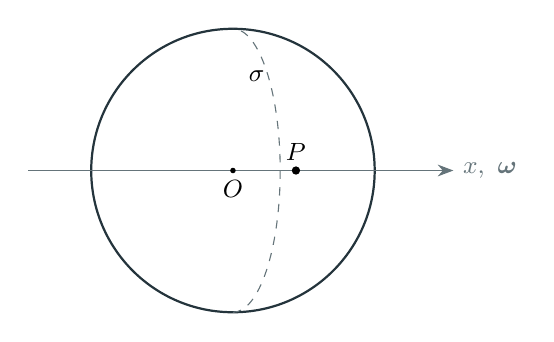
\begin{tikzpicture}[x=1cm,y=1cm]
\draw[object] (0,0) circle(1.8);\draw[axis] (-2.6,0)--(2.8,0) node[right] {$x,\ \vect\omega$};\draw[guide] (0,-1.8) arc(-90:90:.6 and 1.8);\fill (0,0) circle(1pt) node[below] {$O$};\node at (.3,1.2) {$\sigma$};\fill (.8,0) circle(1.5pt) node[above] {$P$};
\end{tikzpicture}\figcaption{图电2.3　旋转轴取水平x轴，P位于球内轴段。}\end{minipage}\end{center}

\Needspace{8\baselineskip}

\pdfbookmark[3]{题型定位}{q3-h0}

\subsection*{题型定位}

旋转面电荷分成绕同一轴转动的圆环，保留观察点坐标进行轴向积分。由积分端点比较球内的平台和球外的衰减。

\Needspace{8\baselineskip}

\pdfbookmark[3]{知识点}{q3-h1}

\subsection*{知识点}

球带面积按递增轴坐标为 $2\pi R\dd x$，用电量除转动周期得 $\dd I=\sigma R\omega\dd x$。圆环轴场分子含 $s^2=R^2-x^2$，分母为到环上各点距离的三次方。

\Needspace{8\baselineskip}

\pdfbookmark[3]{物理图像}{q3-h2}

\subsection*{物理图像}

解图电2.3A中，移动 P 时，球带的半径保持，P 到环中心的距离改为 $p-x$。解图电2.3B表示两个端点到 P 的实际距离；P 跨过球面以后，至少一个根式的取值改变。C图将均匀的轴内场接到两侧同向的偶极尾部。

\Needspace{8\baselineskip}

\pdfbookmark[3]{解题入口}{q3-h3}

\subsection*{解题入口}

从球带宽度 $R\dd\phi$ 写面积、带电量和等效环电流。先在球心直接积分得到 $4/3$，再将一般积分换成 $u=R^2+p^2-2px$。端点平方根分别取实际距离，再将三项差相加。

\Needspace{18\baselineskip}
\pdfbookmark[3]{标准解法}{q3-h4}

\subsection*{标准解法}

把解图电2.3A中的球面按垂直$x$轴的平面切成圆环。环中心坐标为$x$，环半径$s=\sqrt{R^2-x^2}$。取相邻两平面之间轴向坐标的正间距为 $\dd x$。球带沿子午线的宽度为 $R|\dd\phi|$，其中 $x=R\cos\phi$、$s=R\sin\phi$。因此
\[
 \dd S=2\pi sR|\dd\phi|=2\pi R\dd x,
 \qquad \dd I=\frac{\sigma\dd S}{2\pi/\omega}=\sigma R\omega\dd x.
\]
这里 $\dd I$ 的符号由 $\sigma$ 决定。

\begin{center}\begin{minipage}{.98\linewidth}\centering
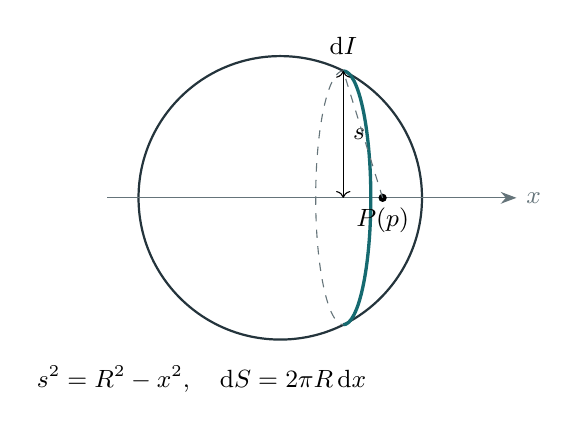
\begin{tikzpicture}[x=1cm,y=1cm]
\draw[object] (0,0) circle(1.8);\draw[axis] (-2.2,0)--(3,0) node[right] {$x$};\draw[very thick,accent] (.8,-1.612) arc(-90:90:.35 and 1.612);\draw[guide] (.8,1.612) arc(90:270:.35 and 1.612);\draw[<->] (.8,0)--(.8,1.612) node[midway,right] {$s$};\fill (1.3,0) circle(1.5pt) node[below] {$P(p)$};\node[above] at (.8,1.7) {$\dd I$};\draw[guide] (1.3,0)--(.8,1.612);\node at (-1,-2.3) {$s^2=R^2-x^2,\quad \dd S=2\pi R\dd x$};
\end{tikzpicture}\figcaption{解图电2.3A　取位于x处的旋转圆环，计算其在轴上$P(p)$处的场。}\end{minipage}\end{center}

在轴上$P=(p,0,0)$，圆环场的横向分量抵消。用递增的$x$作积分变量，得
\[
 B_x(p)=\frac{\mu_0\sigma R\omega}{2}
 \int_{-R}^{R}\frac{R^2-x^2}{(R^2+p^2-2px)^{3/2}}\dd x.
\]
积分分子 $R^2-x^2$ 来自各圆环半径的平方。对$0<|p|<R$，令$u=R^2+p^2-2px$、$A=R^2+p^2$，积分可写为
\[
 \int\frac{R^2-x^2}{u^{3/2}}\dd x
 =-\frac1{8p^3}\left[
 2(R^2-p^2)^2u^{-1/2}+4A u^{1/2}-\frac23u^{3/2}\right].
\]
\Needspace{12\baselineskip}

把方括号中的表达式记为$G(u)$。对应$x=R,-R$的$u$分别为$(R-p)^2,(R+p)^2$。取$|p|<R$，两个根号都是$R\mp p$，故三项的端点差分别给
\begin{align*}
G((R-p)^2)-G((R+p)^2)
&=4p(R^2-p^2)-8p(R^2+p^2)\\
&\quad+4R^2p+\frac43p^3
=-\frac{32}{3}p^3 .
\end{align*}
再乘原函数系数$-1/(8p^3)$，一般$p\ne0$的定积分确为$4/3$。这一步展示了位置参数怎样消去。

在$p=0$，直接积分也得
\[
 \int_{-R}^R\frac{R^2-x^2}{R^3}\dd x=\frac43.
\]
\result{\vect B(P)=\frac23\mu_0\sigma R\vect\omega,\qquad |p|<R.}
结论与$p$无关。球内还可由均匀磁化球的等效面电流得到同一均匀场，但上述圆环积分不依赖这一结论。下面改变端点根号的取值，单独求球外的轴上场。

解图电2.3B把端点取支单独画出。平方根首先是$|R-p|$、$|R+p|$；
只有$|p|<R$时，它们才能同时写成$R-p$、$R+p$。这正是上面端点差抵消位置参数的条件。
轴上各点与球心得到相同的场值，源于圆环积分的端点差。每个圆环仍用图A 所示的实际半径 $s$，满足 $s^2=R^2-x^2$。
\begin{center}\begin{minipage}{.97\linewidth}\centering
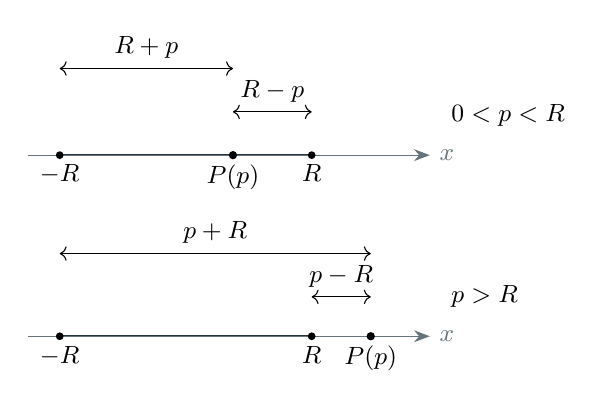
\begin{tikzpicture}[x=1cm,y=1cm,font=\small]
\foreach \h in {0,-2.3}{
\draw[object] (-1.6,\h)--(1.6,\h);
\draw[axis] (-2,\h)--(3.1,\h) node[right] {$x$};
\fill (-1.6,\h) circle(1.4pt) node[below] {$-R$};
\fill (1.6,\h) circle(1.4pt) node[below] {$R$};
}
\fill (.6,0) circle(1.5pt) node[below] {$P(p)$};
\draw[<->] (.6,.55)--(1.6,.55) node[midway,above] {$R-p$};
\draw[<->] (-1.6,1.1)--(.6,1.1) node[midway,above] {$R+p$};
\node[right] at (3.25,.5) {$0<p<R$};
\fill (2.35,-2.3) circle(1.5pt) node[below] {$P(p)$};
\draw[<->] (1.6,-1.8)--(2.35,-1.8) node[midway,above] {$p-R$};
\draw[<->] (-1.6,-1.25)--(2.35,-1.25) node[midway,above] {$p+R$};
\node[right] at (3.25,-1.8) {$p>R$};
\end{tikzpicture}
\figcaption{解图电2.3B　两个端点到轴上P的距离。根号给出绝对值；跨过右端球面后，$|R-p|$ 从 $R-p$ 改为 $p-R$。}
\end{minipage}\end{center}

沿用这一原函数算球外。先取$p>R$，将端点根号改为$p-R$、$p+R$后，
\[
G((p-R)^2)-G((p+R)^2)=-\frac{32}{3}R^3,\qquad
\mathcal I(p)=\frac{4R^3}{3p^3}.
\]
积分核在同时变换$x\to-x,p\to-p$时不变，所以$\mathcal I(-p)=\mathcal I(p)$。
整个轴线的结果因此为
\[
\boldsymbol B(p)=B_0\boldsymbol e_x
\begin{cases}
1,& |p|<R,\\[2pt]
(R/|p|)^3,& |p|>R,
\end{cases}
\qquad B_0=\frac23\mu_0\sigma R\omega.
\]
\begin{center}\begin{minipage}{.97\linewidth}\centering
\begin{tikzpicture}[x=1cm,y=1cm,font=\small]
\fill[accent!8] (-1.2,0) rectangle (1.2,1.8);
\draw[axis] (-3.4,0)--(3.5,0) node[right] {$u=p/R$};
\draw[axis] (0,0)--(0,2.25) node[above] {$B_x/B_0$};
\draw[traj,domain=-2.5:-1,samples=70] plot ({1.2*\x},{1.6/abs(\x)^3});
\draw[traj] (-1.2,1.6)--(1.2,1.6);
\draw[traj,domain=1:2.5,samples=70] plot ({1.2*\x},{1.6/\x^3});
\draw[guide] (-1.2,0)--(-1.2,1.6) (1.2,0)--(1.2,1.6);
\node[above left] at (0,1.6) {$1$};
\node[below] at (-1.2,0) {$-1$};\node[below] at (1.2,0) {$1$};
\node at (.6,.55) {轴内};
\node[above] at (-2.1,.65) {$|u|^{-3}$};
\node[above] at (2.1,.65) {$u^{-3}$};
\end{tikzpicture}
\figcaption{解图电2.3C　整个轴线的真实场，$B_0=2\mu_0\sigma R\omega/3$。两侧轴外场均与轴内场同向，大小按距离三次倒数衰减。}
\end{minipage}\end{center}

解图电2.3C中，两侧轴外的场都与轴内场同向。负电荷或反转转向会使$B_0$变号，整条曲线相应反向。
在极点 $p=R$ 直接积分：令$t=R-x$，原积分化为
\[
\mathcal I(R)=\frac1{(2R)^{3/2}}\int_0^{2R}(2R-t)t^{-1/2}\,\mathrm dt
=\frac43.
\]
端点虽有可积的平方根奇性，总场有限；$p=-R$同理，均接上图中的平台。
这与极点处旋转速度、面电流都为零相符。球面其他位置有面电流，切向磁场的跳跃由当地 $\vect K=\sigma(\vect\omega\times R\vect n)$ 决定。

\Needspace{8\baselineskip}

\pdfbookmark[3]{关键洞察}{q3-h5}

\subsection*{关键洞察}

一般轴内点的位置无关性来自三个端点差的组合。轴外根号改号，结果成为 $|p|^{-3}$。比较纬向面电流后，还可把整个球等效为均匀磁化球，说明均匀性也适用于轴外的球内点。

\Needspace{8\baselineskip}

\pdfbookmark[3]{易错点}{q3-h6}

\subsection*{易错点}

\begin{itemize}
\item 球带面积要用球面斜宽；改成轴向微元时，正面积为 $2\pi R|\dd x|$。
\item 圆环分子取当地 $s^2$，轴上距离平方为 $s^2+(p-x)^2$。
\item 端点根号是 $|R-p|,|R+p|$。中心直接积分；球面极点的积分也有限。
\end{itemize}

\Needspace{8\baselineskip}

\pdfbookmark[3]{课堂讲解建议}{q3-h7}

\subsection*{课堂讲解建议}

在解图电2.3A上标一个窄球带，依次写面积、电量、周期和电流。让学生移动 P，指明积分核中哪些量随 P 变化而哪些量保持。一般积分算完后，用解图电2.3B把 P 从球内沿轴移出去，重新读两个距离，得到图C的轴外尾部。

进阶讲解从变图电2.3V8的球面电流出发，分别写内外磁标势，借表面两个分量的条件求系数。然后用变图电2.3V5比较实体球，说明同一个观察点为何要分两种球壳来积。

\Needspace{18\baselineskip}
\pdfbookmark[3]{变式训练}{q3-h8}

\subsection*{变式训练}

\begin{enumerate}
\item 设总电荷 $Q=4\pi R^2\sigma$。代入轴内平台，得到 $\vect B=\mu_0Q\vect\omega/(6\pi R)$。变图电2.3V1按同一参考球归一化：固定 $Q$ 时，放大半径会把电荷摊到更大的面积上，合场按 $1/R$ 降低；固定 $\sigma$ 时，总电荷随 $R^2$ 增加，合场随 $R$ 增大。
\begin{center}\begin{minipage}{.98\linewidth}\centering
\begin{tikzpicture}[scale=.85,transform shape]
\draw[axis](0,0)--(6.2,0)node[right]{$R/R_*$};\draw[axis](0,0)--(0,3.5)node[above]{$B/B_*$};
\begin{scope}[x=2.34cm,y=1.34cm]
\draw[traj,domain=.49:2.4,samples=75]plot(\x,{1/\x});
\draw[object,dashed](.24,.24)--(2.4,2.4);
\fill(1,1)circle(1.4pt)node[above]{$(1,1)$};
\node[right]at(2.27,.44){固定 $Q$};
\node[above left]at(2.30,2.3){固定 $\sigma$};
\end{scope}
\end{tikzpicture}
\figcaption{变图电2.3V1\quad 以同一参考球归一化，固定总电荷和固定面密度得到不同半径规律}
\end{minipage}\end{center}
\item 把均匀体电荷密度为 $\rho$ 的实心球分成变图电2.3V2中的薄球壳。半径 $s$、厚度 $\dd s$ 的壳对应面密度 $\rho\dd s$，所以壳在球心产生 $\dd\vect B=(2/3)\mu_0\rho s\,\vect\omega\dd s$。所有壳同轴，将 $s$ 从0积到 $R$ 得 $\vect B(0)=\mu_0\rho R^2\vect\omega/3$。
\begin{center}\begin{minipage}{.98\linewidth}\centering
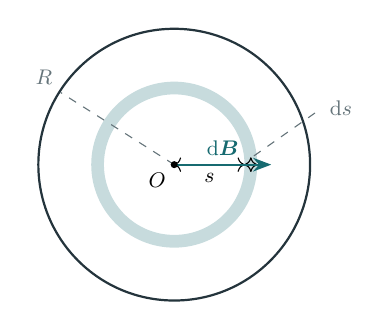
\begin{tikzpicture}[scale=.85,transform shape]
\fill[accent!24,even odd rule](0,0)circle(1.24)(0,0)circle(1.05);
\draw[object](0,0)circle(2.03);
\draw[guide](0,0)--(-1.7,1.08)node[above left]{$R$};
\draw[<->](0,0)--(1.05,0)node[midway,below]{$s$};
\draw[<->](1.05,0)--(1.24,0);
\draw[guide](1.19,.13)--(2.20,.84)node[right]{$\dd s$};
\draw[motion](0,0)--(1.45,0)node[midway,above]{$\dd\vect B$};
\fill(0,0)circle(1.5pt)node[below left]{$O$};
\end{tikzpicture}
\figcaption{变图电2.3V2\quad 实体球分为薄球壳；每个薄壳的中心场沿转轴}
\end{minipage}\end{center}
\item 位于 $x$ 的环有磁矩 $\dd\mu=\dd I\,\pi(R^2-x^2)$。代 $\dd I=\sigma R\omega\dd x$，
\[
\mu=\pi\sigma R\omega\int_{-R}^R(R^2-x^2)\dd x
=\frac43\pi\sigma\omega R^4=\frac{Q\omega R^2}{3}.
\]
偶极轴场为 $\mu_0\mu/(2\pi |p|^3)$。系数与变图电2.3V3的外轴曲线 $B_0(R/|p|)^3$ 相合；这一球面的外场从球面起就按同一偶极式给出。
\begin{center}\begin{minipage}{.98\linewidth}\centering
\begin{tikzpicture}[scale=.85,transform shape]
\draw[axis](0,0)--(6.2,0)node[right]{$|p|/R$};\draw[axis](0,0)--(0,3.5)node[above]{$B/B_0$};
\begin{scope}[x=1.28cm,y=2.6cm]
\draw[object](0,1)--(1,1);
\draw[traj,domain=1:4.46,samples=90]plot(\x,{1/\x^3});
\fill(1,1)circle(1.4pt)node[above right]{球面};
\node[above]at(2.52,.35){偶极尾部};
\node[below]at(1,0){$1$};
\end{scope}
\end{tikzpicture}
\figcaption{变图电2.3V3\quad 外轴场按距离的三次倒数下降}
\end{minipage}\end{center}
\item 常规环电流正比于 $\sigma\omega$。若把 $\omega$ 反号，实际电荷运动方向反转；若把 $\sigma$ 反号而保持运动方向，负电荷的常规电流与原方向相反。变图电2.3V4的中图对应只反转其中一项，场反号；同时反转两项时乘积保持，右图的场与起始图同向。
\begin{center}\begin{minipage}{.98\linewidth}\centering
\begin{tikzpicture}[scale=.85,transform shape]
\draw[guide](0,-.2)--(6.9,-.2);
\foreach \x/\lab/\sgn in {1.0/初始/1,3.42/单独反转/-1,5.84/同时反转/1}{
 \draw[object](\x,1)circle(.72);
 \node[above]at(\x,1.82){\lab};
 \draw[motion](\x,1)--({\x+.60*\sgn},1);
 \fill(\x,1)circle(1.3pt);}
\node at(3.46,.2){三图取同一转轴正向};
\end{tikzpicture}
\figcaption{变图电2.3V4\quad 只反转电荷符号或转向之一，磁场反转；两者同时反转时保持}
\end{minipage}\end{center}
\item 取轴内一点 $p$，令 $q=|p|$。半径 $s<q$ 的壳对它给外轴场，需把壳内平台乘 $(s/q)^3$；$s>q$ 时用壳内平台。分别积分得
\[
B_x(p)=\frac23\mu_0\rho\omega\left[q^{-3}\int_0^q s^4\dd s+\int_q^R s\dd s\right]
=\mu_0\rho\omega(R^2/3-p^2/5).
\]
变图电2.3V5用 $q/R$ 作横坐标，实线由中心 $1/3$ 降到表面 $2/15$。球外各壳都用偶极因子，归一化外场为 $(2/15)(R/q)^3$，与实线在表面连续。
\begin{center}\begin{minipage}{.98\linewidth}\centering
\begin{tikzpicture}[scale=.85,transform shape]
\draw[axis](0,0)--(6.2,0)node[right]{$|p|/R$};\draw[axis](0,0)--(0,3.5)node[above]{$B_x/(\mu_0\rho\omega R^2)$};
\begin{scope}[x=2.55cm,y=8.3cm]
\draw[traj,domain=0:1,samples=65]plot(\x,{1/3-\x^2/5});
\draw[object,dashed,domain=1:2.17,samples=64]plot(\x,{2/(15*\x^3)});
\fill(1,{2/15})circle(1.4pt)node[above right]{$2/15$};
\node[left]at(0,{1/3}){$1/3$};
\node[below]at(1,0){$1$};
\end{scope}
\end{tikzpicture}
\figcaption{变图电2.3V5\quad 均匀体电荷球的轴内场随 $p^2$ 降低，表面接外轴偶极场}
\end{minipage}\end{center}
\item 两同心球面同速转动。从外侧看，两壳磁矩为 $Q_j\omega R_j^2/3$；令 $Q_2=-Q_1 R_1^2/R_2^2$，变图电2.3V6的两个磁矩等大反向，最外部的轴场相消。球心在两壳内部，分别取 $\mu_0Q_j\omega/(6\pi R_j)$，得到
\[
B_x(0)=\frac{\mu_0Q_1\omega}{6\pi R_1}
\left[1-\left(R_1/R_2\right)^3\right].
\]
外部按 $Q_jR_j^2$ 加权，球心按 $Q_j/R_j$ 加权。
\begin{center}\begin{minipage}{.98\linewidth}\centering
\begin{tikzpicture}[scale=.85,transform shape]
\draw[object](0,0)circle(2);
\draw[traj](0,0)circle(1.12);
\draw[axis](-2.55,0)--(3.18,0)node[right]{转轴};
\draw[motion](0,.45)--(1.37,.45)node[above]{$\boldsymbol\mu_1$};
\draw[motion](0,-.45)--(-1.37,-.45)node[below]{$\boldsymbol\mu_2$};
\node[above]at(-1.30,1.66){$R_2$};
\node at(.1,1.38){$R_1$};
\node[right]at(2.25,1.22){外部合场为零};
\end{tikzpicture}
\figcaption{变图电2.3V6\quad 两壳磁矩相反，外场相消；内部场按另一半径权重相加}
\end{minipage}\end{center}
\item 改用 $\sigma(x)=\sigma_0(1+\eta x/R)$，$|\eta|\le1$。球心积分核关于 $x$ 为偶，故奇密度项消失、中心场仍为 $B_0=2\mu_0\sigma_0R\omega/3$。沿轴对积分核求导然后取 $p=0$，得到
\[
B'_x(0)=\frac{3\mu_0\omega R}{2R^5}\int_{-R}^R
\sigma(x)x(R^2-x^2)\dd x .
\]
这里常密度项为奇函数，剩下 $\sigma_0\eta/R$ 乘积分 $4R^5/15$，所以 $B_x'(0)=(2/5)\mu_0\sigma_0\omega\eta$。变图电2.3V7画的是中心切线；$\eta\ne0$ 时，轴内场已随位置变化。
\begin{center}\begin{minipage}{.98\linewidth}\centering
\begin{tikzpicture}[scale=.85,transform shape]
\draw[axis](-2.80,0)--(3.37,0)node[right]{$p$};
\draw[axis](0,0)--(0,3.1)node[above]{$B_x$};
\draw[guide](-2.25,1.55)--(2.42,1.55);
\draw[traj](-1.22,1.19)--(1.22,1.91)node[above right]{中心切线};
\fill(0,1.55)circle(1.4pt)node[above left]{$B_0$};
\node[below right]at(1.65,1.47){$\eta>0$};
\end{tikzpicture}
\figcaption{变图电2.3V7\quad 密度的一阶奇函数项在中心场抵消，却使中心斜率非零}
\end{minipage}\end{center}
\item 变图电2.3V8以转轴为磁标势的极轴。令等效均匀磁化 $\boldsymbol M=\sigma R\boldsymbol\omega$，其表面电流 $\boldsymbol M\times\vect n$ 正好等于旋转面电荷的 $\sigma(\boldsymbol\omega\times R\vect n)$。可用这个等效磁化球确定场。取 $\Phi_{\rm in}=Ar\cos\phi$、$\Phi_{\rm out}=C\cos\phi/r^2$，并令 $\vect H=-\nabla\Phi$。球面无等效自由面电流，切向 $H$ 连续给 $A=C/R^3$；法向 $B$ 连续给 $M-A=2C/R^3$。于是 $A=M/3$，球内 $\vect H=-\boldsymbol M/3$、$\vect B=2\mu_0\boldsymbol M/3$，任一点都相同。球外标势仅含偶极项，磁矩为 $(4\pi R^3/3)\boldsymbol M$。
\begin{center}\begin{minipage}{.98\linewidth}\centering
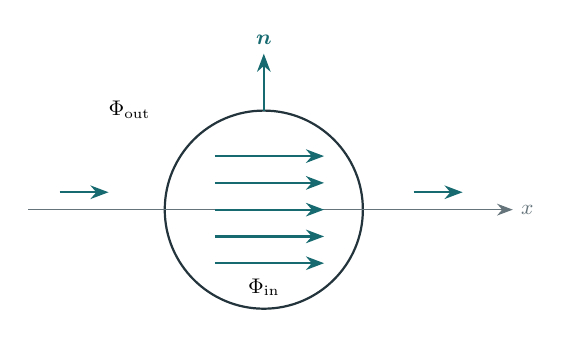
\begin{tikzpicture}[scale=.85,transform shape]
\draw[object](0,0)circle(1.48);
\draw[axis](-3.52,0)--(3.72,0)node[right]{$x$};
\foreach \y in {-.80,-.40,0,.40,.80}{\draw[motion](-.73,\y)--(.90,\y);}
\draw[motion](-3.05,.26)--(-2.32,.26);
\draw[motion](2.24,.26)--(2.97,.26);
\draw[motion](0,1.48)--(0,2.33)node[above]{$\vect n$};
\node[left]at(-1.57,1.49){$\Phi_{\rm out}$};
\node[below]at(0,-.91){$\Phi_{\rm in}$};
\end{tikzpicture}
\figcaption{变图电2.3V8\quad 均匀磁化的等效球：球内场平行，外部轴上场同向}
\end{minipage}\end{center}
\end{enumerate}

\clearpage

\pdfbookmark[2]{第 4 题 无限长螺旋导线的轴上磁场}{q4}

\section*{第 4 题\quad 无限长螺旋导线的轴上磁场}\label{q:4}

真空中一根无限长细导线，沿半径$R$、螺距$H>0$的圆柱面绕成等距螺旋线，电流为$I$。圆柱轴为$y$轴。用参数$\phi$规定导线位置
\[
 \vect r(\phi)=(R\cos\phi,h\phi,R\sin\phi),\qquad h=H/(2\pi),
\]
电流沿$\phi$增大方向。求原点$O$处磁场的三个分量；说明轴上其他点的场怎样变化。

\begin{center}\begin{minipage}{.98\linewidth}\centering
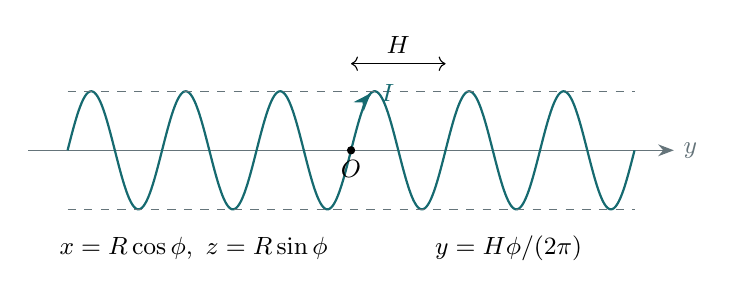
\begin{tikzpicture}[x=1cm,y=1cm]
\draw[axis] (-4.1,0)--(4.1,0) node[right] {$y$};\draw[traj,domain=-1080:1080,samples=360] plot({\x/300},{.75*sin(\x)});\draw[guide] (-3.6,.75)--(3.6,.75);\draw[guide] (-3.6,-.75)--(3.6,-.75);\draw[<->] (0,1.1)--(1.2,1.1) node[midway,above] {$H$};\fill (0,0) circle(1.5pt) node[below] {$O$};\node at (-2,-1.25) {$x=R\cos\phi,\ z=R\sin\phi$};\node at (2,-1.25) {$y=H\phi/(2\pi)$};
\draw[motion,domain=45:75,samples=12] plot({\x/300},{.75*sin(\x)}) node[right] {$I$};
\end{tikzpicture}\figcaption{图电2.4　螺旋线的投影；完整空间方位由参数式规定。}\end{minipage}\end{center}

\Needspace{8\baselineskip}

\pdfbookmark[3]{题型定位}{q4-h0}

\subsection*{题型定位}

在真空中求一根细螺旋线的精确轴上场。先按参数作三维叉乘，再用螺旋平移给轴上其他点的相位。

\Needspace{8\baselineskip}

\pdfbookmark[3]{知识点}{q4-h1}

\subsection*{知识点}

$h=H/(2\pi)$ 是每弧度的轴向位移。切向由圆周方向和 $+y$ 方向相加。毕奥—萨伐尔分母含 $\phi^2$；按分子奇偶性合并 $\phi$ 与 $-\phi$。

\Needspace{8\baselineskip}

\pdfbookmark[3]{物理图像}{q4-h2}

\subsection*{物理图像}

解图电2.4A中，两种电流元分量同起点、同距场点。B图的三条积分核中，只有 $x$ 项在配对后相消。D图中沿轴走四分之一螺距时，两维横向投影交换角色，轴向值保持。

\Needspace{8\baselineskip}

\pdfbookmark[3]{解题入口}{q4-h3}

\subsection*{解题入口}

对给定 $\vect r(\phi)$ 求导，以 $-\vect r$ 作位矢叉乘。先积出含常分子的 $B_y$，再把偶对称的两项合写为 $B_z$ 的收敛积分。场点平移 $y_0$ 后，在原积分中用 $\phi-y_0/h$ 为新变量。

\Needspace{18\baselineskip}
\pdfbookmark[3]{标准解法}{q4-h4}

\subsection*{标准解法}

解图电2.4A把螺旋电流元分为绕轴的圆周分量和沿轴的直线分量。相对于$O$，电流元和源点到场点的位矢分别为
\[
 \dd\vect l=(-R\sin\phi,h,R\cos\phi)\dd\phi,
 \qquad\vect s=-\vect r(\phi),\qquad s^2=R^2+h^2\phi^2.
\]
\begin{center}\begin{minipage}{.97\linewidth}\centering
\begin{tikzpicture}[x=1.5cm,y=1.5cm,font=\small]
\coordinate (O) at (0,0);
\coordinate (S) at (.6516,.9192);
\coordinate (V) at (1.3516,.9192);
\coordinate (W) at (.9733,1.5874);
\coordinate (T) at (1.6733,1.5874);
\draw[axis] (-.4,0)--(2.8,0) node[right] {$y$};
\draw[axis] (O)--(0,2.25) node[above] {$z$};
\draw[axis] (O)--(-1.2,-.65) node[below] {$x$};
\fill (S) circle(1.4pt);
\draw[guide] (S)--(-.35,1.5) node[left] {$S(\phi),\ \boldsymbol r(\phi)$};
\draw[force] (S)--(O) node[midway,left] {$\boldsymbol s$};
\draw[motion] (S)--(V) node[below right] {$\mathrm d\boldsymbol l_y$};
\draw[motion] (S)--(W) node[above left] {$\mathrm d\boldsymbol l_\phi$};
\draw[object,->] (S)--(T) node[right] {$\mathrm d\boldsymbol l$};
\draw[guide] (V)--(T)--(W);
\node[below] at (O) {$O$};
\end{tikzpicture}
\figcaption{解图电2.4A　按$\phi=\pi/4,\ R=h$的真实切向方向作投影，三个电流元箭头共起点S。直线分量沿$+y$，圆周分量在$xz$平面；两者到O的位矢相同。}
\end{minipage}\end{center}

逐分量叉乘，保留两类电流的贡献，有
\[
 \dd\vect l\times\vect s=
 \bigl(hR[\phi\cos\phi-\sin\phi],-R^2,
 hR[\phi\sin\phi+\cos\phi]\bigr)\dd\phi.
\]
为逐项追踪A图中的两个箭头，先写
\[
\mathrm d\boldsymbol l_\phi=(-R\sin\phi,0,R\cos\phi)\,\mathrm d\phi,\qquad
\mathrm d\boldsymbol l_y=(0,h,0)\,\mathrm d\phi.
\]
在同一个位置S，它们与$\boldsymbol s=(-R\cos\phi,-h\phi,-R\sin\phi)$分别叉乘：
\[
\begin{aligned}
\mathrm d\boldsymbol l_\phi\times\boldsymbol s
&=(hR\phi\cos\phi,-R^2,hR\phi\sin\phi)\,\mathrm d\phi,\\
\mathrm d\boldsymbol l_y\times\boldsymbol s
&=(-hR\sin\phi,0,hR\cos\phi)\,\mathrm d\phi.
\end{aligned}
\]
相加才是前面的总电流元叉乘。轴向分量来自圆周电流元；横向分量是圆周电流元与轴向电流元的场之和。
特别在$\phi=0$的交点，圆周电流沿$+z$、源点到O沿$-x$，叉乘给$-y$；
轴向电流沿$+y$，与同一$-x$位矢叉乘给$+z$。这个交点的两个叉乘分别给出轴向负号和横向局部正号。
\begin{center}\begin{minipage}{.97\linewidth}\centering
\begin{tikzpicture}[x=1cm,y=1.3cm,font=\small]
\draw[axis] (-4.4,0)--(4.5,0) node[right] {$\phi$};
\draw[axis] (0,-1.25)--(0,1.4) node[above] {无量纲核};
\draw[force,domain=-4:4,samples=150] plot(\x,{(\x*cos(deg(\x))-sin(deg(\x)))/(1+\x*\x)^1.5});
\draw[guide,domain=-4:4,samples=150] plot(\x,{-1/(1+\x*\x)^1.5});
\draw[traj,domain=-4:4,samples=150] plot(\x,{(\x*sin(deg(\x))+cos(deg(\x)))/(1+\x*\x)^1.5});
\node[right,warm] at (4.8,.8) {$f_x$：奇};
\node[right,muted] at (4.8,.35) {$f_y$：偶};
\node[right,accent] at (4.8,-.1) {$f_z$：偶};
\node[below=9pt] at (-3.1416,0) {$-\pi$};\node[below=9pt] at (3.1416,0) {$\pi$};
\end{tikzpicture}
\figcaption{解图电2.4B　取$R/h=1$画三分量的真实积分核。只有 $x$ 项为奇函数；偶函数 $f_z$ 包含正、负两种区间。}
\end{minipage}\end{center}

解图电2.4B对应
\[
f_x=\frac{\phi\cos\phi-\sin\phi}{(1+\phi^2)^{3/2}},\quad
f_y=-\frac1{(1+\phi^2)^{3/2}},\quad
f_z=\frac{\phi\sin\phi+\cos\phi}{(1+\phi^2)^{3/2}}.
\]
在 $\phi$ 与 $-\phi$ 处，$f_x$ 取反，$f_y$、$f_z$ 各自保持。这个奇偶性对两类电流元的 $x$ 分量分别成立。图 B 取 $R/h=1$；其他半径和螺距下分母也是偶函数。

$x$分量是奇函数，积分为零。$y$分量为
\[
 B_y=-\frac{\mu_0IR^2}{4\pi}\int_{-\infty}^{\infty}
 \frac{\dd\phi}{(R^2+h^2\phi^2)^{3/2}}
 =-\frac{\mu_0 I}{2\pi h}=-\frac{\mu_0 I}{H}.
\]

上述轴向积分中令$u=h\phi/R$，有
\[
 \int_{-\infty}^{\infty}\frac{\dd\phi}{(R^2+h^2\phi^2)^{3/2}}
 =\frac1{hR^2}
 \left[\frac{u}{\sqrt{1+u^2}}\right]_{-\infty}^{\infty}
 =\frac2{hR^2}.
\]
因此负号来自解图电2.4A所对应的绕向，系数来自全轴积分。

解图中$\dd l_\phi=R\dd\phi$、$\dd l_y=h\dd\phi$。将圆周分量均摊成圆环后，轴向场等效为每单位长度$1/H$匝的长螺线管，也可得到$B_y$；这一步只能用于轴向分量。

还可以把圆周电流元对轴向场的等效关系写完整。固定轴坐标$y=h\phi$，
圆周电流元的有向长度为$R\,\mathrm d\phi$。它到O的距离只取决于$R,y$，
而它的叉乘在轴上的$y$分量恒为$-R\,\mathrm dl_\phi$，不随绕轴方位变化。
因此，仅就这一分量，可把同一个$I\,\mathrm dl_\phi$均摊在该高度的整个圆周上。等效圆环电流满足
\[
\mathrm dI'\,2\pi R=I\,\mathrm dl_\phi,\qquad
\mathrm dI'=\frac{I\,\mathrm d\phi}{2\pi}
=\frac I H\,\mathrm dy.
\]
相邻高度$\mathrm dy$之间连续排置这样的圆环，电流与轴长之比为$I/H$。
若形式上把每段高度看作一匝，则$n=1/\mathrm dy$、每匝电流为$\mathrm dI'$，
乘积$n\,\mathrm dI'=I/H$有限。无限长螺线管的轴向场于是给出
\[
B_{1y}=-\mu_0 n\,\mathrm dI'=-\frac{\mu_0I}{H}.
\]
这与直接积分一致。上述平均没有搬动轴坐标，只消去了同一高度的方位；
算横向场时保留线元的实际方位。下面的 $B_{1z}$、$B_{2z}$ 分别来自圆周和轴向电流元。

由A图两式分别抽出$z$分量，在$s^2=R^2+h^2\phi^2$下，
\[
\begin{aligned}
\mathrm dB_{1z}
&=\frac{\mu_0I}{4\pi}\frac{hR\phi\sin\phi}{s^3}\,\mathrm d\phi,\\
\mathrm dB_{2z}
&=\frac{\mu_0I}{4\pi}\frac{hR\cos\phi}{s^3}\,\mathrm d\phi.
\end{aligned}
\]
第一式来自圆周电流与轴向距离$y=h\phi$的结合；第二式来自轴向电流元
$\mathrm dl_y=h\,\mathrm d\phi$和到轴的径向距离R，再向固定$z$轴投影。
两个核都随 $\phi$ 改变符号，局部贡献按相应的 $\sin\phi$ 和 $\cos\phi$ 取正、负。
分母变为
\[
s^3=\left(\frac H{2\pi}\right)^3
\left[\left(\frac{2\pi R}{H}\right)^2+\phi^2\right]^{3/2}.
\]
故圆周与直线两部分分别积分得
\[
\begin{aligned}
B_{1z}&=\frac{2\pi\mu_0IR}{H^2}\int_0^\infty
\frac{\phi\sin\phi}{[(2\pi R/H)^2+\phi^2]^{3/2}}\,\mathrm d\phi,\\
B_{2z}&=\frac{2\pi\mu_0IR}{H^2}\int_0^\infty
\frac{\cos\phi}{[(2\pi R/H)^2+\phi^2]^{3/2}}\,\mathrm d\phi.
\end{aligned}
\]
两行的因子2均来自偶对称，相加得到总 $B_z$。
$|\phi|\to\infty$时，第一项至多按$\phi^{-2}$、第二项按$\phi^{-3}$衰减，两个积分都绝对收敛。

上述两个 $z$ 分量的积分核均为偶函数，合并得
\[
 B_z=\frac{\mu_0IhR}{2\pi}\int_0^\infty
 \frac{\phi\sin\phi+\cos\phi}{(R^2+h^2\phi^2)^{3/2}}\dd\phi.
\]
\Needspace{16\baselineskip}
换成螺距后，完整答案为
\result{B_x=0,\quad B_y=-\frac{\mu_0 I}{H},\quad
 B_z=\frac{2\pi\mu_0IR}{H^2}\int_0^\infty
 \frac{\phi\sin\phi+\cos\phi}{[(2\pi R/H)^2+\phi^2]^{3/2}}\dd\phi.}
上式就是细螺旋横场的收敛积分。轴向分量由安匝密度给出，横向分量还保留真实绕线相位。

用闭合的安培环路也能求轴向场。先把螺旋绕成一个半径L的大环，
选$2\pi L=NH$使N匝完整闭合；各处的局部圆柱轴线就是大环的切线。
\begin{center}\begin{minipage}{.97\linewidth}\centering
\begin{tikzpicture}[x=1cm,y=1cm,font=\small]
\draw[object] (0,0) circle(1.7) (0,0) circle(2.7);
\draw[guide] (0,0) circle(2.2);
\foreach \ang in {0,45,...,315}{
\node at (\ang:1.7) {$\otimes$};
\node at (\ang:2.7) {$\odot$};
\draw[thin,muted] (\ang:1.86)--(\ang:2.54);
}
\draw[motion] (10:2.2) arc(10:65:2.2);
\draw[<->] (0,0)--(135:2.2) node[midway,above] {$L$};
\node[right,align=left] at (3.4,1) {沿圆柱轴线的环路\\内侧穿入$NI$\\外侧电流在环路之外};
\node at (0,-3.2) {$2\pi L=NH,\qquad L/R\to\infty$};
\end{tikzpicture}
\figcaption{解图电2.4C　先把细螺旋闭合成大环再取小曲率极限。图示八匝的穿入、穿出关系；推导中N趋大。安培环路只提取沿轴的切向分量。}
\end{minipage}\end{center}

解图电2.4C沿这条轴线取安培回路。对图中定向，回路围住N股穿入电流，外侧穿出电流位于回路以外。
有限N时切向场不必沿回路处处相同，先记它的弧长平均为$\overline B_{\rm tan}$，则
\[
\oint\boldsymbol B\cdot\mathrm d\boldsymbol l
=\overline B_{\rm tan}\,2\pi L=-\mu_0 NI,\qquad
\overline B_{\rm tan}=-\frac{\mu_0 NI}{2\pi L}=-\frac{\mu_0I}{H}.
\]
随后令$N\to\infty$、$L/R\to\infty$，局部曲率趋零，才回到题设的无限长直圆柱螺旋。
直圆柱螺旋的轴向分量由螺旋平移对称处处相同，因而极限中的平均值就是所求$B_y$。
先闭合有限大环，再取曲率趋零极限，环路定理的闭合条件始终满足。
该环路的切向与局部轴线重合，点积只提取轴向分量。

沿轴移至$P=(0,y_0,0)$，令$\phi_0=y_0/h$，再以$\phi-\phi_0$作积分变量。轴向分量不变，横向矢量绕$y$轴旋转相应方位：
\[
 \vect B(P)=-\frac{\mu_0I}{H}\vect e_y
 +B_z(O)(-\sin\phi_0\vect e_x+\cos\phi_0\vect e_z).
\]
转角正负按题设参数式确定。

解图电2.4D把最后一个向量式画在四个相隔四分之一螺距的轴上位置。
$y_0=0,H/4,H/2,3H/4$分别给$\phi_0=0,\pi/2,\pi,3\pi/2$，
横向场依次沿$+z,-x,-z,+x$，轴向场都沿$-y$。每经过H，两个横向分量共同回到原值。
\begin{center}\begin{minipage}{.97\linewidth}\centering
\begin{tikzpicture}[x=1cm,y=1cm,font=\small]
\draw[axis] (-2.1,0)--(2.15,0) node[right] {$x$};
\draw[axis] (0,-2)--(0,2.1) node[above] {$z$};
\draw[guide] (0,0) circle(1.4);
\draw[motion] (0,0)--(0,1.4) node[right] {$y_0=0$};
\draw[force] (0,0)--(-1.4,0) node[above] {$H/4$};
\draw[motion] (0,0)--(0,-1.4) node[right] {$H/2$};
\draw[force] (0,0)--(1.4,0) node[below] {$3H/4$};
\node[align=left] at (4.1,.5) {$|\boldsymbol B_\perp|$固定\\$B_y=-\mu_0I/H$固定\\沿轴一螺距转一周};
\end{tikzpicture}
\figcaption{解图电2.4D　在同一原点比较四个不同轴上位置的横向场方向，各箭头不是同处叠加。相位按题设参数增加；$H/4$处横场由$+z$转向$-x$。}
\end{minipage}\end{center}

从参数式也能直接说明这一点：平移到$y_0$后，令$\psi=\phi-\phi_0$，
相对场点的轴向坐标变为$h\psi$，横截面位置则由$\psi$变成$\psi+\phi_0$。
两个积分具有同一分母，横向结果按这一方位共同转动。横向矢量长度保持，每过四分之一螺距，两分量轮流经过零点。

当螺距越来越大，近轴的一段导线渐近平行于轴。令$a=R/h=2\pi R/H$、$\phi=at$，则横向积分可重写成
\[
B_z(O)=\frac{\mu_0I}{2\pi R}F(a),\quad
F(a)=\int_0^\infty\frac{\cos(at)}{(1+t^2)^{3/2}}\,\mathrm dt
+a\int_0^\infty\frac{t\sin(at)}{(1+t^2)^{3/2}}\,\mathrm dt.
\]
对任意 $a>0$，还可以从这个积分确定 $B_z(O)$ 的正号。记第一项为 $C(a)$，则第二项为 $-aC'(a)$。利用高斯积分，先把分母改写为
\[
(1+t^2)^{-3/2}=\frac{2}{\sqrt\pi}\int_0^\infty s^{1/2}e^{-(1+t^2)s}\dd s.
\]
代入 $C$，按 $t$ 先积分，用 $\int_0^\infty e^{-st^2}\cos(at)\dd t=\sqrt\pi e^{-a^2/(4s)}/(2\sqrt s)$，得到
\[
F(a)=C(a)-aC'(a)
=\int_0^\infty\left(1+\frac{a^2}{2s}\right)e^{-s-a^2/(4s)}\dd s>0.
\]
故 $I>0$ 时，解图电2.4D 在 $y_0=0$ 处的横场确实沿 $+z$。此正号适用于任意正螺距。

当$H\to\infty$即$a\to0$时，第一项由可积核给出1，第二项的绝对值不超过
$a\int_0^\infty t(1+t^2)^{-3/2}\mathrm dt=a$，所以
\[
B_y\to0,\qquad B_z(O)\to\frac{\mu_0I}{2\pi R}.
\]
随螺距增大，最靠近 $O$ 的导线逐渐接近距轴 $R$、平行 $y$ 轴的长直线。

\Needspace{8\baselineskip}

\pdfbookmark[3]{关键洞察}{q4-h5}

\subsection*{关键洞察}

轴向值由每轴长的安匝数决定。保留导线方位时，横向矢量随螺旋相位转动且长度恒定。尽管其积分核局部有负值，合场仍有确定的正向幅度。令 $a=R/h>0$，
\[
J_0=\int_0^\infty\frac{\cos\phi\,\mathrm d\phi}{(a^2+\phi^2)^{3/2}},\qquad
J_1=\int_0^\infty\frac{\phi\sin\phi\,\mathrm d\phi}{(a^2+\phi^2)^{3/2}}.
\]
把分母写为高斯参数积分，
\[
(a^2+\phi^2)^{-3/2}
=\frac2{\sqrt\pi}\int_0^\infty t^{1/2}e^{-t(a^2+\phi^2)}\,\mathrm dt.
\]
再用$\int_0^\infty e^{-t\phi^2}\cos\phi\,\mathrm d\phi
=\sqrt\pi e^{-1/(4t)}/(2\sqrt t)$，并对余弦的频率求导得到含$\phi\sin\phi$的一式，得
\[
J_0=\int_0^\infty e^{-a^2t-1/(4t)}\,\mathrm dt>0,\qquad
J_1=\frac12\int_0^\infty t^{-1}e^{-a^2t-1/(4t)}\,\mathrm dt>0.
\]
两积分绝对收敛，可以交换积分次序。对 $I>0$，$J_0,J_1$ 均给正向总贡献，因此解图电2.4D的起始横场沿 $+z$。

\Needspace{8\baselineskip}

\pdfbookmark[3]{易错点}{q4-h6}

\subsection*{易错点}

\begin{itemize}
\item 题给的绕线方向使 $B_y<0$；用 $\phi=0$ 处的叉乘读这个负号。
\item $\dd l_\phi,\dd l_y$ 在同一源点，使用同一条位矢。
\item 圆周和轴向电流元分别给 $z$ 核的 $\phi\sin\phi$、$\cos\phi$ 两项。
\item 固定 $I$ 与固定 $I/H$ 是两种不同的变螺距过程。
\end{itemize}

\Needspace{8\baselineskip}

\pdfbookmark[3]{课堂讲解建议}{q4-h7}

\subsection*{课堂讲解建议}

先用解图电2.4A写出同一线元的两部分，请两组分别算叉乘。回到B图，逐个指出哪些核随 $\phi$ 改号、哪些在 $\phi$ 与 $-\phi$ 取相同值。让学生用一次轴向积分得到 $-\mu_0I/H$，再说明圆周平均保留了哪个分量。

用D图复述平移 $H/4$ 后的场向。最后从变图电2.4V5推广到V6，把每根导线的横向单位矢量乘以电流后相加，比较仅两个相位相反与许多相位均匀两种安排。

\Needspace{18\baselineskip}
\pdfbookmark[3]{变式训练}{q4-h8}

\subsection*{变式训练}

\begin{enumerate}
\item 导线的空间参数式保持，电流沿反方向流动。把 $I$ 看作有符号电流时，这相当于 $I\to-I$，毕奥—萨伐尔积分各分量同时反号。变图电2.4V1中 O 处的场由 $B_y<0,B_z>0$ 转为 $B_y>0,B_z<0$，两种接法均有 $B_x=0$。若改变的是绕线方向，先按新的空间曲线重写 $\vect r(\phi)$。
\begin{center}\begin{minipage}{.98\linewidth}\centering
\begin{tikzpicture}[scale=.85,transform shape]
\draw[axis](0,.25)--(0,3.76)node[above]{$z$};
\draw[axis](-2.9,1.95)--(3.04,1.95)node[right]{$y$};
\draw[motion](0,1.95)--(-1.85,3.09)node[above left]{$I>0$};
\draw[motion](0,1.95)--(1.85,.81)node[below right]{反向通电};
\draw[guide](-1.85,1.95)--(-1.85,3.09)--(0,3.09);
\draw[guide](1.85,1.95)--(1.85,.81)--(0,.81);
\end{tikzpicture}
\figcaption{变图电2.4V1\quad 在原点，反向通电使轴向与横向分量同时反号}
\end{minipage}\end{center}
\item 同时把 $R,H$ 放大 $s$ 倍，保持同一电流。对应的 $\dd\vect l$ 和源点到场点的位矢均乘 $s$，叉乘乘 $s^2$、距离三次方乘 $s^3$。因此在对应的位置处 $\vect B_s=\vect B_1/s$，如变图电2.4V2。$R/H$ 保持，横场积分中的无量纲参数也保持。单改 $H$ 时该参数随之改变，应使用新的积分。
\begin{center}\begin{minipage}{.98\linewidth}\centering
\begin{tikzpicture}[scale=.85,transform shape]
\draw[axis](0,0)--(6.18,0)node[right]{$s$};\draw[axis](0,0)--(0,3.52)node[above]{$|\vect B_s|/|\vect B_1|$};
\begin{scope}[x=2.3cm,y=1.48cm]
\draw[traj,domain=.51:2.5,samples=71]plot(\x,{1/\x});
\fill(1,1)circle(1.4pt)node[above right]{$(1,1)$};
\fill(2,.5)circle(1.4pt)node[above right]{$(2,1/2)$};
\end{scope}
\end{tikzpicture}
\figcaption{变图电2.4V2\quad 半径与螺距一起缩放，整个磁场按同一倒数倍率变化}
\end{minipage}\end{center}
\item 沿轴移动 $\Delta y$ 时，横向相位增加 $\Delta y/h$。变图电2.4V3画出 O、$H/4$ 与 $H$ 处的横向场：移动 $H$ 增相位 $2\pi$，完整场回到原值；移动 $H/4$ 增相位 $\pi/2$，横场由 $+z$ 转到 $-x$，大小相同。轴向分量始终为 $-\mu_0I/H$。
\begin{center}\begin{minipage}{.98\linewidth}\centering
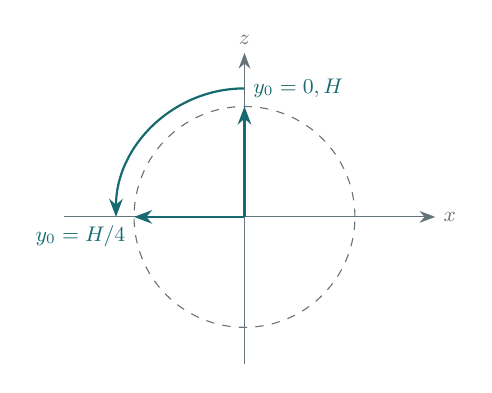
\begin{tikzpicture}[scale=.85,transform shape]
\draw[axis](-2.7,0)--(2.85,0)node[right]{$x$};\draw[axis](0,-2.2)--(0,2.45)node[above]{$z$};
\draw[guide](0,0)circle(1.65);
\draw[motion](0,0)--(0,1.65)node[above right]{$y_0=0,H$};
\draw[motion](0,0)--(-1.65,0)node[below left]{$y_0=H/4$};
\draw[motion](0,1.92)arc(90:180:1.92);
\end{tikzpicture}
\figcaption{变图电2.4V3\quad 沿轴移动一个螺距，横场回到原方向；四分之一螺距对应四分之一周}
\end{minipage}\end{center}
\item 在同一柱面上叠加均匀相位的同绕向螺旋，电流总量为 $I_{\rm tot}$，各相位等权。变图电2.4V4中每个横向矢量与其相反相位配对。连续极限下，$\int_0^{2\pi}\sin\delta\,\dd\delta=\int_0^{2\pi}\cos\delta\,\dd\delta=0$，只剩相加的轴向场 $-\mu_0 I_{\rm tot}/H$。横场的消去由这个源分布的均匀相位给出。
\begin{center}\begin{minipage}{.98\linewidth}\centering
\begin{tikzpicture}[scale=.85,transform shape]
\draw[axis](-2.7,0)--(2.85,0)node[right]{$x$};\draw[axis](0,-2.2)--(0,2.45)node[above]{$z$};
\draw[guide](0,0)circle(1.63);
\foreach \a in {0,30,...,330}{\draw[motion](0,0)--(\a:1.63);}
\node[above right]at(1.39,1.64){均匀相位};
\node[below right]at(1.33,-1.46){横向相加为零};
\end{tikzpicture}
\figcaption{变图电2.4V4\quad 均匀相位的等权横场矢量成对抵消}
\end{minipage}\end{center}
\item 两根螺旋相差 $\pi$、各通 $I/2$。如变图电2.4V5，同一轴点上的两横场分别正比于 $(-\sin\phi_0,\cos\phi_0)$ 及 $(\sin\phi_0,-\cos\phi_0)$，相加为零；轴向两项同为 $-\mu_0I/(2H)$，合成 $-\mu_0I/H$。这一配对用到了场点在共同轴上；轴外点到两根线的距离分布各自按实际几何计算。
\begin{center}\begin{minipage}{.98\linewidth}\centering
\begin{tikzpicture}[scale=.85,transform shape]
\draw[axis](-2.7,0)--(2.85,0)node[right]{$x$};\draw[axis](0,-2.2)--(0,2.45)node[above]{$z$};
\draw[guide](0,0)circle(1.38);
\draw[motion](0,0)--(0,1.38)node[above right]{$\delta=0$};
\draw[motion](0,0)--(0,-1.38)node[below right]{$\delta=\pi$};
\draw[object](-2.35,-1.8)circle(5pt);
\draw[object](-2.43,-1.88)--(-2.27,-1.72);
\draw[object](-2.43,-1.72)--(-2.27,-1.88);
\node[right]at(-2.21,-1.8){两根的轴向场同向};
\end{tikzpicture}
\figcaption{变图电2.4V5\quad 相差半周的两根等流导线，横场相消，轴向场相加}
\end{minipage}\end{center}
\item 同半径、同螺距，定义 $\kappa=B_z(O)/I$。相位为 $\delta_j$ 的第 $j$ 根线给
\[
\boldsymbol B_\perp=\kappa\sum_j I_j
(-\sin\delta_j\,\boldsymbol e_x+\cos\delta_j\,\boldsymbol e_z),
\qquad B_y=-\frac{\mu_0}{H}\sum_j I_j .
\]
要使横场消失，两项加权三角和都为零。变图电2.4V6举 $0,\pi/2,\pi$ 三相分别通 $2I_*,I_*,I_*$ 的例子，所得横向合场为 $\kappa I_*(-\boldsymbol e_x+\boldsymbol e_z)$，可由图中剩余的两个等长投影读出。
\begin{center}\begin{minipage}{.98\linewidth}\centering
\begin{tikzpicture}[scale=.85,transform shape]
\draw[axis](-2.7,0)--(2.85,0)node[right]{$x$};\draw[axis](0,-2.2)--(0,2.45)node[above]{$z$};
\draw[motion](0,0)--(0,1.86)node[above right]{$2I_*$};
\draw[motion](0,0)--(0,-.93)node[below right]{$I_*$};
\draw[motion](0,0)--(-.93,0)node[below left]{$I_*$};
\draw[motion](0,0)--(-.93,.93)node[above left]{合横场};
\draw[guide](0,.93)--(-.93,.93)--(-.93,0);
\end{tikzpicture}
\figcaption{变图电2.4V6\quad 相位与电流一起决定横向场；矢量长度按各线电流取值}
\end{minipage}\end{center}
\item 固定安匝密度 $J=I/H$ 和半径 $R$，让 $H\to0$。轴向场保持为 $-\mu_0J$。对主解 $F(a)$ 的正弦项分部积分，$t(1+t^2)^{-3/2}$ 在两端都趋零，其导数为 $(1-2t^2)/(1+t^2)^{5/2}$。于是
\[
F(a)=\int_0^\infty\frac{2-t^2}{(1+t^2)^{5/2}}\cos(at)\,\dd t .
\]
核的绝对积分不超过 $2\int_0^\infty(1+t^2)^{-3/2}\dd t=2$，故 $|B_z|/(\mu_0J)=|F(a)|/a\le2/a$。变图电2.4V7中 $a$ 向右增大，横场趋零而轴向场保持。若改为固定 $I$，轴向场大小随 $1/H$ 增长。
\begin{center}\begin{minipage}{.98\linewidth}\centering
\begin{tikzpicture}[scale=.85,transform shape]
\draw[axis](0,0)--(6.18,0)node[right]{$a=R/h$};\draw[axis](0,0)--(0,3.52)node[above]{归一化场};\draw[traj]plot coordinates {(0.65000,2.48077) (0.71059,2.26372) (0.77118,2.07729) (0.83176,1.91492) (0.89235,1.77185) (0.95294,1.64457) (1.01353,1.53038) (1.07412,1.42724) (1.13471,1.33350) (1.19529,1.24788) (1.25588,1.16933) (1.31647,1.09700) (1.37706,1.03017) (1.43765,0.96824) (1.49824,0.91072) (1.55882,0.85718) (1.61941,0.80724) (1.68000,0.76060) (1.74059,0.71696) (1.80118,0.67609) (1.86176,0.63776) (1.92235,0.60178) (1.98294,0.56798) (2.04353,0.53620) (2.10412,0.50630) (2.16471,0.47815) (2.22529,0.45164) (2.28588,0.42666) (2.34647,0.40311) (2.40706,0.38089) (2.46765,0.35994) (2.52824,0.34016) (2.58882,0.32149) (2.64941,0.30387) (2.71000,0.28722) (2.77059,0.27150) (2.83118,0.25665) (2.89176,0.24262) (2.95235,0.22936) (3.01294,0.21683) (3.07353,0.20499) (3.13412,0.19380) (3.19471,0.18322) (3.25529,0.17321) (3.31588,0.16376) (3.37647,0.15482) (3.43706,0.14636) (3.49765,0.13837) (3.55824,0.13081) (3.61882,0.12367) (3.67941,0.11691) (3.74000,0.11052) (3.80059,0.10448) (3.86118,0.09877) (3.92176,0.09337) (3.98235,0.08826) (4.04294,0.08343) (4.10353,0.07886) (4.16412,0.07454) (4.22471,0.07046) (4.28529,0.06660) (4.34588,0.06295) (4.40647,0.05950) (4.46706,0.05623) (4.52765,0.05315) (4.58824,0.05023) (4.64882,0.04747) (4.70941,0.04486) (4.77000,0.04240) (4.83059,0.04006) (4.89118,0.03786) (4.95176,0.03578) (5.01235,0.03381) (5.07294,0.03195) (5.13353,0.03019) (5.19412,0.02852) (5.25471,0.02695) (5.31529,0.02546) (5.37588,0.02406) (5.43647,0.02273) (5.49706,0.02147) (5.55765,0.02029) (5.61824,0.01917) (5.67882,0.01811) (5.73941,0.01710) (5.80000,0.01616)};
\draw[object,dashed](0,1.52)--(5.8,1.52)node[right]{$|B_y|/(\mu_0J)$};
\node[right]at(3.10,.82){$|B_z|/(\mu_0J)$};
\end{tikzpicture}
\figcaption{变图电2.4V7\quad 固定安匝密度时，轴向场保持而横向场随螺距减小趋零}
\end{minipage}\end{center}
\item 固定 $I,R$，让 $H$ 很大。变图电2.4V8的横轴 $a=2\pi R/H$ 趋零，归一化轴向场大小为 $a$，横场为 $F(a)\to1$。因此 $B_y\to0$、$B_z\to\mu_0I/(2\pi R)$。距 O 最近的一段线趋近平行 $+y$、离轴为 $R$；若起始相位是 $\delta$，该段横向位置随 $\delta$ 转动，按右手定则得到 $-\sin\delta\,\boldsymbol e_x+\cos\delta\,\boldsymbol e_z$ 的场向。
\begin{center}\begin{minipage}{.98\linewidth}\centering
\begin{tikzpicture}[scale=.85,transform shape]
\draw[axis](0,0)--(6.18,0)node[right]{$a=2\pi R/H$};\draw[axis](0,0)--(0,3.52)node[above]{场相对 $\mu_0 I/(2\pi R)$};\draw[traj]plot coordinates {(0.00000,2.25000) (0.08999,2.25202) (0.17998,2.25643) (0.26998,2.26231) (0.35997,2.26919) (0.44996,2.27673) (0.53995,2.28470) (0.62994,2.29291) (0.71994,2.30122) (0.80993,2.30949) (0.89992,2.31763) (0.98991,2.32556) (1.07990,2.33319) (1.16990,2.34048) (1.25989,2.34736) (1.34988,2.35380) (1.43987,2.35977) (1.52987,2.36522) (1.61986,2.37014) (1.70985,2.37451) (1.79984,2.37831) (1.88983,2.38152) (1.97983,2.38415) (2.06982,2.38617) (2.15981,2.38760) (2.24980,2.38842) (2.33979,2.38863) (2.42979,2.38824) (2.51978,2.38725) (2.60977,2.38567) (2.69976,2.38349) (2.78975,2.38074) (2.87975,2.37740) (2.96974,2.37351) (3.05973,2.36905) (3.14972,2.36405) (3.23971,2.35852) (3.32971,2.35246) (3.41970,2.34588) (3.50969,2.33881) (3.59968,2.33125) (3.68967,2.32321) (3.77967,2.31471) (3.86966,2.30575) (3.95965,2.29637) (4.04964,2.28655) (4.13963,2.27633) (4.22963,2.26571) (4.31962,2.25470) (4.40961,2.24333) (4.49960,2.23159) (4.58960,2.21952) (4.67959,2.20711) (4.76958,2.19438) (4.85957,2.18134) (4.94956,2.16801) (5.03956,2.15441) (5.12955,2.14053) (5.21954,2.12640) (5.30953,2.11202) (5.39952,2.09741) (5.48952,2.08258) (5.57951,2.06754) (5.66950,2.05231)};\draw[object,dashed]plot coordinates {(0.00000,0.00000) (0.08999,0.05179) (0.17998,0.10357) (0.26998,0.15536) (0.35997,0.20714) (0.44996,0.25893) (0.53995,0.31071) (0.62994,0.36250) (0.71994,0.41429) (0.80993,0.46607) (0.89992,0.51786) (0.98991,0.56964) (1.07990,0.62143) (1.16990,0.67321) (1.25989,0.72500) (1.34988,0.77679) (1.43987,0.82857) (1.52987,0.88036) (1.61986,0.93214) (1.70985,0.98393) (1.79984,1.03571) (1.88983,1.08750) (1.97983,1.13929) (2.06982,1.19107) (2.15981,1.24286) (2.24980,1.29464) (2.33979,1.34643) (2.42979,1.39821) (2.51978,1.45000) (2.60977,1.50179) (2.69976,1.55357) (2.78975,1.60536) (2.87975,1.65714) (2.96974,1.70893) (3.05973,1.76071) (3.14972,1.81250) (3.23971,1.86429) (3.32971,1.91607) (3.41970,1.96786) (3.50969,2.01964) (3.59968,2.07143) (3.68967,2.12321) (3.77967,2.17500) (3.86966,2.22679) (3.95965,2.27857) (4.04964,2.33036) (4.13963,2.38214) (4.22963,2.43393) (4.31962,2.48571) (4.40961,2.53750) (4.49960,2.58929) (4.58960,2.64107) (4.67959,2.69286) (4.76958,2.74464) (4.85957,2.79643) (4.94956,2.84821) (5.03956,2.90000) (5.12955,2.95179) (5.21954,3.00357) (5.30953,3.05536) (5.39952,3.10714) (5.48952,3.15893) (5.57951,3.21071) (5.66950,3.26250)};
\fill(0,2.25)circle(1.4pt)node[left]{$1$};
\node[above]at(3.18,2.35){横场};
\node[below right]at(4.3,2.43){$|B_y|$};
\end{tikzpicture}
\figcaption{变图电2.4V8\quad 螺距趋无限大时，对应横轴原点，横场趋直线电流的场}
\end{minipage}\end{center}
\end{enumerate}

\clearpage

\pdfbookmark[2]{第 5 题 互补圆柱导体空隙中的均匀磁场}{q5}

\section*{第 5 题\quad 互补圆柱导体空隙中的均匀磁场}\label{q:5}

两根无限长非磁性导体沿$z$轴方向放置，截面互为镜像。构造截面的两个圆直径均为$D$，圆心$C_+=(-D/4,0)$、$C_-=(D/4,0)$；每根导体占据自身圆盘去掉两圆重叠透镜区后的部分。重叠区为空隙。两导体分别均匀通有沿$+z$和$-z$方向的电流$I$，每根截面积为$A=(\pi/12+\sqrt3/8)D^2$。求空隙内任意点$(x,y)$的磁场。

\begin{center}\begin{minipage}{.98\linewidth}\centering
\begin{tikzpicture}[x=1cm,y=1cm]
\begin{scope}\clip (-3,-2) rectangle(3,2);\fill[accent!15] (-.6,0) circle(1.2);\fill[warm!15] (.6,0) circle(1.2);\begin{scope}\clip (-.6,0) circle(1.2);\fill[white] (.6,0) circle(1.2);\end{scope}\end{scope}
\draw[object] (-.6,0) circle(1.2);\draw[object] (.6,0) circle(1.2);\fill (-.6,0) circle(1pt) node[below left] {$C_+$};\fill (.6,0) circle(1pt) node[below right] {$C_-$};\node at (-1.1,.45) {$\odot I$};\node at (1.1,.45) {$\otimes I$};\node[fill=white,inner sep=1pt] at (0,.7) {空隙};\draw[axis] (-2,0)--(2,0) node[right] {$x$};\draw[axis] (0,-1.5)--(0,1.6) node[above] {$y$};
\end{tikzpicture}\figcaption{图电2.5　重叠透镜区没有实际电流，左右月牙区电流反向。}\end{minipage}\end{center}

\Needspace{8\baselineskip}

\pdfbookmark[3]{题型定位}{q5-h0}

\subsection*{题型定位}

先补全两个月牙形载流截面，把源分布还原成可用安培定律求场的两个圆柱，再求透镜空隙的共同内部场。

\Needspace{8\baselineskip}

\pdfbookmark[3]{知识点}{q5-h1}

\subsection*{知识点}

均匀载流圆柱内部 $\vect B=(\mu_0j/2)\vect e_z\times\vect s$。完整圆柱总电流按 $I^\prime=j\pi r^2$，月牙总电流按 $I=jA$。两正负补流在重叠区逐点抵消。

\Needspace{8\baselineskip}

\pdfbookmark[3]{物理图像}{q5-h2}

\subsection*{物理图像}

解图电2.5A中两个相对位矢都指向同一个 P。两者之差从左圆心指向右圆心，P 移动时保持。解图电2.5C把两内部场放在同一个起点，水平分量相消、合场沿正 $y$。

\Needspace{8\baselineskip}

\pdfbookmark[3]{解题入口}{q5-h3}

\subsection*{解题入口}

先按解图电2.5B用两个扇形减两个三角形算透镜面积，确定实际截面与 $j=I/A$。然后用 $\vect s_+-\vect s_-=\vect C_--\vect C_+$ 合并两个内部场。等值反向的源补流使计算模型和实际空隙对应。

\Needspace{18\baselineskip}
\pdfbookmark[3]{标准解法}{q5-h4}

\subsection*{标准解法}

解图电2.5A把左导体补成完整圆柱，重叠区附加正向电流密度$j=I/A$；右导体也补成完整圆柱，重叠区附加负向电流密度$-j$。这两项在空隙处相消，因而完整双圆柱模型与实际电流分布相同。

\begin{center}\begin{minipage}{.98\linewidth}\centering
\begin{tikzpicture}[x=1cm,y=1cm]
\draw[object] (-.7,0) circle(1.4);\draw[object] (.7,0) circle(1.4);\coordinate (P) at (.1,.55);
\fill (-.7,0) circle(1.2pt) node[below left] {$C_+$};\fill (.7,0) circle(1.2pt) node[below right] {$C_-$};\fill (P) circle(1.5pt) node[above] {$P$};\draw[motion] (-.7,0)--(P) node[midway,left] {$\vect s_+$};\draw[force] (.7,0)--(P) node[midway,right] {$\vect s_-$};\draw[very thick,->] (2.7,-.6)--(2.7,.8) node[above] {$\vect B$};\node at (0,-1.9) {$\vect s_+-\vect s_-=\frac D2\vect e_x$};\node at (-1.25,-.65) {$+j$};\node at (1.25,-.65) {$-j$};
\end{tikzpicture}\figcaption{解图电2.5A　补成两个完整均匀圆柱，空隙中的虚构电流逐点相消。}\end{minipage}\end{center}

用两圆相交的几何关系求月牙截面积。令$r=D/2$，解图电2.5B的两轴间距为r。
连结$C_+$、$C_-$与上交点T，得到边长r的等边三角形；上、下交点对左圆心张角$2\pi/3$。
透镜由两个相同的圆弓形组成，故
\[
S_{\rm lens}=2\left[\frac12r^2\frac{2\pi}{3}
-\frac12r^2\sin\frac{2\pi}{3}\right]
=\left(\frac{2\pi}{3}-\frac{\sqrt3}{2}\right)r^2.
\]
\begin{center}\begin{minipage}{.97\linewidth}\centering
\begin{tikzpicture}[x=1cm,y=1cm,font=\small]
\fill[accent!10] (-.7,0) circle(1.4);
\fill[warm!10] (.7,0) circle(1.4);
\begin{scope}\clip (-.7,0) circle(1.4);\fill[white] (.7,0) circle(1.4);\end{scope}
\draw[object] (-.7,0) circle(1.4) (.7,0) circle(1.4);
\coordinate (L) at (-.7,0);\coordinate (R) at (.7,0);
\coordinate (T) at (0,1.2124);\coordinate (U) at (0,-1.2124);
\draw[guide] (L)--(T)--(R)--(U)--(L);
\fill (L) circle(1.3pt) node[below left] {$C_+$};
\fill (R) circle(1.3pt) node[below right] {$C_-$};
\fill (T) circle(1.3pt) node[above] {$T$};
\fill (U) circle(1.3pt) node[below] {$U$};
\draw (-.525,-.3031) arc(-60:60:.35);
\node at (.12,0) {$2\pi/3$};
\draw[<->] (-2.1,-1.85)--(.7,-1.85) node[midway,below] {$D=2r$};
\node[above left] at (-.4,.65) {$r$};
\node at (0,1.9) {$|C_+C_-|=r=D/2$};
\end{tikzpicture}
\figcaption{解图电2.5B　两圆半径为$r=D/2$、轴距也为r，透镜对应两个$2\pi/3$扇形减去两个三角形。左右月牙才是实际导体。}
\end{minipage}\end{center}

从一个完整圆中扣去透镜，解图电2.5B的一个月牙面积为
\[
A=\pi r^2-S_{\rm lens}
=\left(\frac\pi3+\frac{\sqrt3}{2}\right)r^2
=\left(\frac{\pi}{12}+\frac{\sqrt3}{8}\right)D^2.
\]
实际月牙内总电流为I，所以$j=I/A$。补全截面时沿用电流密度 $j$，因此完整圆柱的总电流增至 $I^\prime=j\pi r^2$。
两者关系也可从面积比先写出
\[
\frac{I}{I'}=\frac{A}{\pi D^2/4}
=\frac{2\pi+3\sqrt3}{6\pi}.
\]

完整圆柱的电流为
\[
 I'=j\frac{\pi D^2}{4}=\frac{6\pi I}{2\pi+3\sqrt3}.
\]
半径$D/2$的均匀轴向电流圆柱，在内部距自身轴线位矢$\vect s$处，由安培环路定律
\[
 B(2\pi s)=\mu_0 j\pi s^2,\qquad
 \vect B=\frac{\mu_0j}{2}\vect e_z\times\vect s.
\]
重叠区任意点同时位于两完整圆柱内部。相对两圆心的位矢为
\[
 \vect s_+=(x+D/4)\vect e_x+y\vect e_y,
 \quad\vect s_-=(x-D/4)\vect e_x+y\vect e_y.
\]
于是
\begin{align*}
 \vect B_+&=\frac{\mu_0j}{2}[-y\vect e_x+(x+D/4)\vect e_y],\\
 \vect B_-&=-\frac{\mu_0j}{2}[-y\vect e_x+(x-D/4)\vect e_y].
\end{align*}
\Needspace{10\baselineskip}

还可以在不展开坐标的情况下先看出消去原因：在解图电2.5A，同一点$P$的两个相对位矢满足
\[
\vect s_+-\vect s_-=\vect C_- -\vect C_+=\frac D2\vect e_x .
\]
因此$\vect B_++\vect B_-=(\mu_0j/2)\vect e_z\times(D\vect e_x/2)$，对空隙内任意$P$都相同。这里之所以两项均用内部场，是因为$P$同时落在两个完整圆柱内。

相加后含$x,y$的项全部消失：
\result{\vect B=\frac{\mu_0jD}{4}\vect e_y
 =\frac{6\mu_0 I}{(2\pi+3\sqrt3)D}\vect e_y.}
所以空隙中是匀强场。一般地，两相反均匀电流圆柱的共同内部区域，有$\vect B=(\mu_0j/2)\vect e_z\times(\vect C_--\vect C_+)$；均匀性来自内部场对位矢的线性关系。

解图电2.5C把同一点的两个分场画在一起。正向左柱在P给
$B_{+x}=-\mu_0jy/2$，负向右柱给$B_{-x}=+\mu_0jy/2$，水平分量逐点抵消。
两者的竖直分量之和为
\[
\frac{\mu_0j}{2}\left(x+\frac D4\right)
-\frac{\mu_0j}{2}\left(x-\frac D4\right)
=\frac{\mu_0jD}{4}.
\]
\begin{center}\begin{minipage}{.97\linewidth}\centering
\begin{tikzpicture}[x=1cm,y=1cm,font=\small]
\draw[guide] (-.7,0) circle(1.4) (.7,0) circle(1.4);
\coordinate (P) at (.1,.55);
\coordinate (A) at (-.45,1.35);
\coordinate (B) at (.65,1.15);
\coordinate (S) at (.1,1.95);
\fill (P) circle(1.4pt) node[below] {$P$};
\fill (-.7,0) circle(1.2pt) node[below left] {$C_+$};
\fill (.7,0) circle(1.2pt) node[below right] {$C_-$};
\draw[motion] (P)--(A) node[above left,fill=white,inner sep=1pt] {$\boldsymbol B_+$};
\draw[force] (P)--(B) node[right] {$\boldsymbol B_-$};
\draw[object,->] (P)--(S) node[above] {$\boldsymbol B\parallel+y$};
\draw[guide] (A)--(S)--(B);
\node at (0,-1.95) {两箭头水平分量相反，竖直分量相加};
\end{tikzpicture}
\figcaption{解图电2.5C　取与A图相同的P，各磁场按共同正比例缩放。两分场与合场同起点；P 点的两分场叠加给空隙中的合场。}
\end{minipage}\end{center}

移动P时，A图两条相对位矢都增加同一个位移，它们的差保持不变；
C图两个分场的坐标项因而继续约消，得到同一合场。空隙中 $\nabla\times\boldsymbol B=0$。这里还得到更强的结论：两个完整圆柱的内部场对相对位矢呈线性，因电流密度大小相等、方向相反，位置项逐点相消，留下常矢量。
离开两圆公共内部区后，至少一个圆柱要改用外部场公式，刚才的线性约消不再适用。

逐区读解图电2.5A：左月牙为 $+j$，右月牙为 $-j$，透镜内补入的两项相消，两圆外两项都是零。因此两完整柱的总电流分布处处等于实际月牙分布，磁场可由完整柱场相加。

\Needspace{8\baselineskip}

\pdfbookmark[3]{关键洞察}{q5-h5}

\subsection*{关键洞察}

均匀性来自内部场对相对位矢的线性及相反的等大电流密度。共同内部区的场只由两轴间位移决定；走出共同区后，改用相应圆柱的外部公式。

\Needspace{8\baselineskip}

\pdfbookmark[3]{易错点}{q5-h6}

\subsection*{易错点}

\begin{itemize}
\item $D$ 是直径，两个圆心相距 $D/2$。
\item 计算完整柱的场时沿用月牙的电流密度 $j$；两者总电流用各自面积换算。
\item P 对两完整柱都在内部；右柱的负电流使其场式整体反号。
\end{itemize}

\Needspace{8\baselineskip}

\pdfbookmark[3]{课堂讲解建议}{q5-h7}

\subsection*{课堂讲解建议}

把解图电2.5A分成两张透明圆盘，在左月牙、透镜、右月牙、两圆外各取一点，分别读两张图的电流密度并相加。确认补全后的分布后，再让学生不展开坐标，用两个指向同一点的位矢说明合场为何处处相同。

在两个圆心的中点画两场，读出正 $y$ 方向；随后改成变图电2.5V7的不同密度，要求学生指出应在透镜补回哪种电流，为什么对称中心的修正场为零。

\Needspace{18\baselineskip}
\pdfbookmark[3]{变式训练}{q5-h8}

\subsection*{变式训练}

\begin{enumerate}
\item 变图电2.5V1中令 $\vect d=\vect C_--\vect C_+$。两个相反等密度的完整柱在共同内部的场为 $\frac{\mu_0j}{2}\vect e_z\times(\vect r-\vect C_+)$ 与 $-\frac{\mu_0j}{2}\vect e_z\times(\vect r-\vect C_-)$。相加得到
\[
\vect B=\frac{\mu_0j}{2}\vect e_z\times\vect d,\qquad B=\frac{\mu_0jd}{2}.
\]
共同内部存在的条件为 $d<R_++R_-$；中心距和半径决定透镜形状，场只含 $\vect d$。
\begin{center}\begin{minipage}{.98\linewidth}\centering
\begin{tikzpicture}[scale=.85,transform shape]
\begin{scope}
\clip (-0.82,0)circle(1.32);
\fill[accent!22](0.82,0)circle(1.32);
\end{scope}
\draw[object](-0.82,0)circle(1.32);\draw[traj](0.82,0)circle(1.32);
\fill(-0.82,0)circle(1.38pt)node[below left]{$C_+$};
\fill(0.82,0)circle(1.38pt)node[below right]{$C_-$};
\draw[<->](-.82,-1.62)--(.82,-1.62)node[midway,below]{$d$};
\fill(0,.44)circle(1.4pt)node[right]{$P$};
\draw[guide](-.82,0)--(0,.44)--(.82,0);
\draw[motion](0,.44)--(0,1.8)node[above]{$\vect B$};
\end{tikzpicture}
\figcaption{变图电2.5V1\quad 共同区域的合场由两圆柱轴距确定}
\end{minipage}\end{center}
\item 若叠加的是两个完整圆柱，分别取 $+j_1,-j_2$，则共同区中的场为
\[
\vect B=\frac{\mu_0}{2}\vect e_z\times
\bigl[(j_1-j_2)\vect r-j_1\vect C_++j_2\vect C_-\bigr].
\]
变图电2.5V2取 $y=0$ 的两个点，$j_1>j_2$ 时向右移动，$B_y$ 按 $\partial_x B_y=\mu_0(j_1-j_2)/2$ 增加。$j_1=j_2$ 时位置项消失。这个共同区实际有净电流密度 $j_1-j_2$；月牙形导体的真实空隙需加透镜修正，见变图电2.5V7。
\begin{center}\begin{minipage}{.98\linewidth}\centering
\begin{tikzpicture}[scale=.85,transform shape]
\begin{scope}
\clip (-0.57,0)circle(1.32);
\fill[accent!22](0.57,0)circle(1.32);
\end{scope}
\draw[object](-0.57,0)circle(1.32);\draw[traj](0.57,0)circle(1.32);
\fill(-0.57,0)circle(1.38pt)node[below left]{$C_+$};
\fill(0.57,0)circle(1.38pt)node[below right]{$C_-$};
\fill(-.37,0)circle(1.4pt)node[below]{$P_1$};
\fill(.37,0)circle(1.4pt)node[below]{$P_2$};
\draw[motion](-.37,0)--(-.37,.7);
\draw[motion](.37,0)--(.37,1.29);
\node[right]at(1.85,.80){$j_1>j_2$};
\end{tikzpicture}
\figcaption{变图电2.5V2\quad 数学叠加的两柱密度不同时，共同区域的场随位置变化}
\end{minipage}\end{center}
\item 直接给定 $j$ 时，用变图电2.5V3的 $\vect d=(D/2)\vect e_x$，得到 $\vect B=\mu_0jD\vect e_y/4$。若还需求电源供给一个月牙的总电流，再把密度乘以它的导电面积 $A$，即 $I=jA$；补全圆的总电流按其更大的圆盘面积求。
\begin{center}\begin{minipage}{.98\linewidth}\centering
\begin{tikzpicture}[scale=.85,transform shape]
\begin{scope}
\clip (-0.72,0)circle(1.32);
\fill[accent!22](0.72,0)circle(1.32);
\end{scope}
\draw[object](-0.72,0)circle(1.32);\draw[traj](0.72,0)circle(1.32);
\fill(-0.72,0)circle(1.38pt)node[below left]{$C_+$};
\fill(0.72,0)circle(1.38pt)node[below right]{$C_-$};
\node at(-1.46,.54){$+j$};\node at(1.48,.54){$-j$};
\draw[motion](0,.05)--(0,1.53)node[above]{$\mu_0jD/4$};
\draw[<->](-.72,-1.55)--(.72,-1.55)node[midway,below]{$D/2$};
\end{tikzpicture}
\figcaption{变图电2.5V3\quad 已知电流密度和轴距即可求场，月牙面积用于换算总电流}
\end{minipage}\end{center}
\item 两个导体同时反向，相当于电流密度处处乘 $-1$。所以变图电2.5V4的场从 $+\vect e_y$ 变为 $-\vect e_y$，大小仍为 $\mu_0jD/4$，且位置项继续相消。若只把右导体反向至 $+j$，两个补全柱同向，在真实透镜空隙里需再减去密度 $+2j$ 的透镜电流；同向完整柱自身的位置项则相加。
\begin{center}\begin{minipage}{.98\linewidth}\centering
\begin{tikzpicture}[scale=.85,transform shape]
\foreach \x/\sgn in {0/1,5.15/-1}{
\begin{scope}[xshift=\x cm]
\draw[object](-1,0)circle(1.32);
\draw[object](1,0)circle(1.32);
\fill(0,0)circle(1.5pt);
\draw[motion](0,0)--(0,{1.25*\sgn});
\end{scope}}
\node at(0,-1.88){起始电流};
\node at(5.15,-1.88){两根都反向};
\end{tikzpicture}
\figcaption{变图电2.5V4\quad 两股电流一起反向时，空隙中合场反号，大小保持}
\end{minipage}\end{center}
\item 如变图电2.5V5，取 $|R_+-R_-|<d<R_++R_-$ 形成部分重叠。扣除相同透镜后，两实际截面面积一般不同。各通等幅反向密度 $+j,-j$ 时，补全产生的透镜电流仍相消；两个内部场相加仍为 $\frac{\mu_0j}{2}\vect e_z\times\vect d$。实际供电电流要按各面积选择，$I_+/I_-=A_+/A_-$。
\begin{center}\begin{minipage}{.98\linewidth}\centering
\begin{tikzpicture}[scale=.85,transform shape]
\begin{scope}
\clip(-.91,0)circle(1.67);
\fill[accent!21](.88,0)circle(1.19);
\end{scope}
\draw[object](-.91,0)circle(1.67);
\draw[traj](.88,0)circle(1.19);
\fill(-.91,0)circle(1.4pt)node[below left]{$C_+$};
\fill(.88,0)circle(1.4pt)node[below right]{$C_-$};
\draw[<->](-.91,-1.95)--(.88,-1.95)node[midway,below]{$d$};
\node at(-1.69,.75){$+j$};\node at(1.31,.54){$-j$};
\draw[motion](.25,.04)--(.25,1.57)node[above]{$\vect B$};
\end{tikzpicture}
\figcaption{变图电2.5V5\quad 构造两圆半径不同，等幅反向的补流在共同区域仍相消}
\end{minipage}\end{center}
\item 在大圆柱中挖一个偏心圆孔。变图电2.5V6的 $\vect d=\vect C'-\vect C$ 从柱心指向孔心。用完整大圆柱的 $+j$ 与孔位置的小圆柱 $-j$ 叠加，孔内正负电流相消，场等于
\[
\frac{\mu_0j}{2}\vect e_z\times[(\vect r-\vect C)-(\vect r-\vect C')]
=\frac{\mu_0j}{2}\vect e_z\times\vect d.
\]
若大、小半径为 $a,b$，取 $|\vect d|+b<a$ 保证整孔在大圆柱内部。图中合场从 $\vect d$ 在截面内按右手方向转90度。
\begin{center}\begin{minipage}{.98\linewidth}\centering
\begin{tikzpicture}[scale=.85,transform shape]
\fill[accent!22,even odd rule](0,0)circle(1.96)(.73,.44)circle(.85);
\draw[object](0,0)circle(1.96);
\draw[traj](.73,.44)circle(.85);
\fill(0,0)circle(1.5pt)node[below]{$C$};
\fill(.73,.44)circle(1.5pt)node[right]{$C'$};
\draw[motion](0,0)--(.73,.44)node[midway,below right]{$\vect d$};
\draw[motion](.73,.44)--(.14,1.42)node[above left]{$\vect B$};
\node at(-1.14,.60){$+j$};
\end{tikzpicture}
\figcaption{变图电2.5V6\quad 偏心孔中的场垂直于两轴位移，大小只取决于位移和电流密度}
\end{minipage}\end{center}
\item 密度不等的实际空隙，需要在完整两柱叠加之外再补变图电2.5V7的透镜电流 $j_2-j_1$。O处，一对关于 O 中心对称的透镜源元到 O 的位矢相反，给出的场正好抵消。故
\[
\vect B(O)=\frac{\mu_0D(j_1+j_2)}8\vect e_y .
\]
对其他 P，补流场可按横截面 $\mathcal L$ 写成
\[
\delta\vect B(P)=\frac{\mu_0(j_2-j_1)}{2\pi}\int_{\mathcal L}
\frac{\vect e_z\times(\vect r-\vect r')}{|\vect r-\vect r'|^2}\,\dd^2r' .
\]
将它与完整双柱的场相加，才能同时恢复零电流密度和空隙的实际场。
\begin{center}\begin{minipage}{.98\linewidth}\centering
\begin{tikzpicture}[scale=.85,transform shape]
\begin{scope}
\clip (-0.68,0)circle(1.32);
\fill[accent!22](0.68,0)circle(1.32);
\end{scope}
\draw[object](-0.68,0)circle(1.32);\draw[traj](0.68,0)circle(1.32);
\fill(-0.68,0)circle(1.38pt)node[below left]{$C_+$};
\fill(0.68,0)circle(1.38pt)node[below right]{$C_-$};
\draw[axis](-2.25,0)--(2.36,0)node[right]{$x$};
\fill(0,0)circle(1.45pt)node[below]{$O$};
\node[above]at(0,.55){补 $j_2-j_1$};
\draw[guide](-.24,.44)--(.24,-.44);
\fill(-.24,.44)circle(1.4pt);
\fill(.24,-.44)circle(1.4pt);
\node[left]at(-.24,.44){$-\vect r^\prime$};
\node[right]at(.24,-.44){$\vect r^\prime$};
\end{tikzpicture}
\figcaption{变图电2.5V7\quad 补入的透镜电流关于 O 中心对称，对 O 的场两两相消}
\end{minipage}\end{center}
\item 令正电荷以 $v\vect e_z$ 从 $(x_0,y_0)$ 射入，磁场沿 $+\vect e_y$。初始洛伦兹力沿 $-x$，所以变图电2.5V8中圆心在 $x_0-r_L$，其中 $r_L=mv/(qB)$。在固定的 $y=y_0$ 剖面内，
\[
x_{\rm left}=\frac D4-\sqrt{\frac{D^2}4-y_0^2},
\qquad x_{\rm right}=-\frac D4+\sqrt{\frac{D^2}4-y_0^2}.
\]
回旋轨道横坐标从 $x_0-2r_L$ 到 $x_0$。要求其始终在空隙内，取 $x_0-2r_L>x_{\rm left}$ 且 $x_0<x_{\rm right}$；若达到等号，轨道会与导体表面接触。
\begin{center}\begin{minipage}{.98\linewidth}\centering
\begin{tikzpicture}[scale=.85,transform shape]
\draw[axis](-2.8,0)--(2.82,0)node[right]{$x$};
\draw[axis](0,-1.58)--(0,2.02)node[above]{$z$};
\draw[guide](-2.07,-1.51)--(-2.07,1.77);
\draw[guide](2.07,-1.51)--(2.07,1.77);
\draw[traj](-.38,.35)circle(1.02);
\fill(.64,.35)circle(1.5pt)node[below right]{$x_0$};
\draw[motion](.64,.35)--(.64,1.53)node[right]{$v\vect e_z$};
\draw[motion](.64,.35)--(-.38,.35)node[midway,above]{$r_L$};
\node[below left]at(-2.07,-.95){$x_{\rm left}$};
\node[below right]at(2.07,-.95){$x_{\rm right}$};
\node at(-.63,-1.32){定高 $y_0$};
\end{tikzpicture}
\figcaption{变图电2.5V8\quad 在固定高度的剖面内，整条回旋轨迹要位于两道导体侧界之间}
\end{minipage}\end{center}
\end{enumerate}

\clearpage

\pdfbookmark[2]{第 6 题 有限厚电流层的磁场分布}{q6}

\section*{第 6 题\quad 有限厚电流层的磁场分布}\label{q:6}

真空中$-d\le x\le d$的无限平面层沿$y,z$方向无限延伸，层内均匀电流密度为$\vect j=j\vect e_z$，其中$j>0$。无其他外加磁场。求全空间的磁感应强度分布。

\begin{center}\begin{minipage}{.98\linewidth}\centering
\begin{tikzpicture}[x=1cm,y=1cm]
\fill[accent!10] (-1.4,-1.5) rectangle(1.4,1.5);\draw[object] (-1.4,-1.5)--(-1.4,1.5);\draw[object] (1.4,-1.5)--(1.4,1.5);\foreach \x in {-1,0,1}\foreach \y in {-.8,0,.8}\node at (\x,\y) {$\odot$};\draw[axis] (-2.7,-1.9)--(2.7,-1.9) node[right] {$x$};\node[below] at (-1.4,-1.9) {$-d$};\node[below] at (1.4,-1.9) {$d$};\node at (0,1.9) {$\vect j=j\vect e_z$};
\end{tikzpicture}\figcaption{图电2.6　截面中圆点表示向外的电流；层沿y和z无限延伸。}\end{minipage}\end{center}

\Needspace{8\baselineskip}

\pdfbookmark[3]{题型定位}{q6-h0}

\subsection*{题型定位}

有限厚度的无限平面电流层。先定场向，再用逐渐加宽的安培矩形得层内线性支、层外平台。

\Needspace{8\baselineskip}

\pdfbookmark[3]{知识点}{q6-h1}

\subsection*{知识点}

对 $y,z$ 平移不变；平行 $z$ 的各细线场在 $xy$ 平面。镜像配对和无散定律都给出 $B_x=0$。安培回路的穿流截面积取实际载流宽度乘长边，微分形式为 $\dd B_y/\dd x=\mu_0j_z$。

\Needspace{8\baselineskip}

\pdfbookmark[3]{物理图像}{q6-h2}

\subsection*{物理图像}

解图电2.6B中回路的两长边行进反向、磁场也反向，点积相加；宽度超过 $2d$ 后，包围的载流宽度固定。解图电2.6C显示场在层面连续，而斜率从 $\mu_0j$ 变成零。

\Needspace{8\baselineskip}

\pdfbookmark[3]{解题入口}{q6-h3}

\subsection*{解题入口}

先按直线电流分解和镜像配对求场向，用中面对称给 $B_y(0)=0$。再让解图电2.6B的一对长边从层内移动到层外，分别写穿过回路的电流，合并成三段函数。

\Needspace{18\baselineskip}
\pdfbookmark[3]{标准解法}{q6-h4}

\subsection*{标准解法}

先确定场的方向，再求大小。将体电流分解成平行$z$轴的直线电流，每根线在场点的磁场都在$xy$平面内，故$B_z=0$。关于经过场点的$xz$平面对称的两根线，其$x$分量相消、$y$分量相加，因此只剩$B_y(x)$。解图电2.6A的高斯盒也能给出法向分量，并显示各面对净磁通的贡献。

电流分布在$y,z$方向具有平移对称性，所以本层产生的场只依赖$x$。将整个电流层绕$z$轴转过$180^\circ$，电流分布不变；
场的两个平面分量随之反向，再用y方向的平移不变性，得到
\[
B_x(-x)=-B_x(x),\qquad B_y(-x)=-B_y(x).
\]
以上奇性针对题设无外加磁场时电流层产生的场；叠加均匀场后，总场一般不再具有这一奇性。
\begin{center}\begin{minipage}{.97\linewidth}\centering
\begin{tikzpicture}[x=1cm,y=1cm,font=\small]
\draw[object] (-1.65,-.875)--(1.15,-.875)--(1.15,.525)--(-1.65,.525)--cycle;
\draw[guide] (-1.15,-.525)--(1.65,-.525)--(1.65,.875)--(-1.15,.875)--cycle;
\draw[object] (-1.65,-.875)--(-1.15,-.525) (1.15,-.875)--(1.65,-.525)
(1.15,.525)--(1.65,.875) (-1.65,.525)--(-1.15,.875);
\draw[force] (1.4,0)--(2.65,0) node[right] {$B_x(x_0)$};
\draw[force] (-1.4,0)--(-2.65,0) node[left] {$-B_x(x_0)$};
\draw[guide] (1.45,.6)--(2.2,1.2) node[right] {$\Delta S\ (yz\text{面})$};
\node[below] at (-1.4,-.9) {$-x_0$};
\node[below] at (1.4,-.9) {$x_0$};
\node at (0,1.65) {两$z$面通量为零，两$y$面通量相消};
\end{tikzpicture}
\figcaption{解图电2.6A　边沿$x,y,z$方向的闭合高斯盒。仅画法向场分量 $B_x$。两侧外法线和场分量均反向，故两通量同号，由无散定律得 $B_x=0$。}
\end{minipage}\end{center}

取解图电2.6A的盒子，x侧面在$\pm x_0$，每个$yz$侧面的面积为$\Delta S$。
将六面磁通按法线方向归类：
\[
0=\iint_{\partial V}\boldsymbol B\cdot\mathrm d\boldsymbol S
=\Phi_{xy}+\Phi_{xz}+\Phi_{yz}.
\]
两个$xy$面法线沿z，而$B_z=0$，所以$\Phi_{xy}=0$。
两个$xz$面法线沿$\pm y$，同一x处的$B_y(x)$不依赖y，通量成对相消，所以$\Phi_{xz}=0$；
若利用上面的奇性，也可直接看到各面上$\int_{-x_0}^{x_0}B_y(x)\,\mathrm dx=0$。
于是只剩两个$yz$面：
\[
\Phi_{yz}=[B_x(x_0)-B_x(-x_0)]\Delta S
=2B_x(x_0)\Delta S=0,\qquad B_x(x_0)=0.
\]
A图左、右两面的外法线和待定场分量同时反向，两个点积同号，和为一个面的两倍。无散定律要求它们都为零；任意$x_0$均成立，因而全空间只有$B_y(x)$。

\begin{center}\begin{minipage}{.97\linewidth}\centering
\begin{tikzpicture}[x=1cm,y=1cm,font=\small]
\fill[accent!8] (-.8,-1.4) rectangle(.8,1.4);
\draw[axis] (-2.65,0)--(2.9,0) node[right] {$x$};
\draw[axis] (0,-1.5)--(0,1.75) node[above] {$y$};
\draw[object] (-1.6,-1)--(1.6,-1)--(1.6,1)--(-1.6,1)--cycle;
\draw[motion] (-.9,-1)--(.9,-1);
\draw[motion] (.9,1)--(-.9,1);
\draw[force] (1.6,-.6)--(1.6,.6) node[right] {$B_y(x)$};
\draw[force] (-1.6,.6)--(-1.6,-.6) node[left] {$-B_y(x)$};
\draw[<->] (4,-1)--(4,1) node[pos=.85,right] {$\ell$};
\node[below] at (-1.6,-1) {$-x$};\node[below] at (1.6,-1) {$x$};
\node[below] at (-.8,0) {$-d$};\node[below] at (.8,0) {$d$};
\foreach \xx in {-.4,.4}\foreach \yy in {-.65,.65}\node at (\xx,\yy) {$\odot$};
\end{tikzpicture}
\figcaption{解图电2.6B　安培回路在$xy$平面，正向对应法线$+z$。两条竖边长度为$\ell$，水平间距为$2x$；图示$x>d$，载流宽度只到$2d$。}
\end{minipage}\end{center}


取解图电2.6B中关于$x=0$对称的矩形安培回路，其两长边平行$y$轴、长$\ell$，位于$\pm x$。按图选回路方向，$x>0$侧磁场沿正$y$轴，两长边环量相加。
当$0\le x\le d$时，包围电流为$j(2x\ell)$，故
\[
 2B_y(x)\ell=\mu_0 j(2x\ell),\qquad B_y(x)=\mu_0jx.
\]
当$x\ge d$时，包围电流不再随回路加宽而增加：
\[
 2B_y(x)\ell=\mu_0j(2d\ell),\qquad B_y(x)=\mu_0jd.
\]
利用奇对称性补齐负半空间，得
\result{\vect B(x)=\begin{cases}
 -\mu_0jd\vect e_y,&x<-d,\\
 \mu_0jx\vect e_y,&|x|\le d,\\
 \mu_0jd\vect e_y,&x>d.
 \end{cases}}

\begin{center}\begin{minipage}{.97\linewidth}\centering
\begin{tikzpicture}[x=1cm,y=1cm,font=\small]
\fill[accent!7] (-1.5,-1.45) rectangle(1.5,1.45);
\draw[axis] (-3.4,0)--(3.45,0) node[right] {$u=x/d$};
\draw[axis] (0,-1.65)--(0,1.8) node[above] {$B_y/(\mu_0jd)$};
\draw[traj] (-3,-1.2)--(-1.5,-1.2)--(1.5,1.2)--(3,1.2);
\draw[guide] (-1.5,0)--(-1.5,-1.2)--(0,-1.2) (1.5,0)--(1.5,1.2)--(0,1.2);
\node[below] at (-1.5,0) {$-1$};\node[below] at (1.5,0) {$1$};
\node[left] at (0,1.2) {$1$};\node[left] at (0,-1.2) {$-1$};
\node at (.7,-1.4) {载流层};
\end{tikzpicture}
\figcaption{解图电2.6C　归一化场曲线。对应的$B_y(x)$在层内斜率为$\mu_0j$，层外斜率为零；$x=\pm d$处场连续，斜率改变。阴影只标对应的载流横坐标区间。}
\end{minipage}\end{center}
在解图电2.6C的右侧层面，内侧极限$B_y(d^-)=\mu_0jd$与外侧极限$B_y(d^+)=\mu_0jd$相同；左侧同理。导数则从层内$\mu_0j$变成层外0。有限体电流密度的阶跃改变场的斜率；场在无额外面电流的层面连续通过。

也可把体电流分成薄片，按薄片在两侧的场分量相加。厚$\dd x'$的薄层等效面电流为$\dd K=j\dd x'$，在其右侧给$+\mu_0\dd K/2$的$y$分量，左侧给相反分量。对层内点$x$，
\[B_y(x)=\frac{\mu_0j}{2}\left[
\int_{-d}^{x}\dd x'-\int_x^d\dd x'\right]
=\mu_0jx.\]
对$x>d$，所有薄层都给同向贡献，得到$\mu_0j(2d)/2=\mu_0jd$。解图电2.6C中场的线性支与平台支由此都能解释，都由薄片累计的电流给出。

C图同时给出方向和大小：右半空间$B_y>0$，左半空间$B_y<0$；层内大小随$|x|$增加，层外大小恒定。若叠加均匀外场，对称回路只能求出两长边的场差；题设的无外场条件才确定这里的绝对场值。

\Needspace{8\baselineskip}

\pdfbookmark[3]{关键洞察}{q6-h5}

\subsection*{关键洞察}

厚度有限的体电流使 $B_y$ 连续；穿过已有集中面电流时，$\dd B_y/\dd x$ 在该面有集中项，场按 $\mu_0 K$ 跳变。无限层的层外平台来自移动回路后载流宽度保持不变。

\Needspace{8\baselineskip}

\pdfbookmark[3]{易错点}{q6-h6}

\subsection*{易错点}

\begin{itemize}
\item 两长边的环量同号，短边因与 B 垂直而贡献零。
\item 层内回路包围宽 $2x$，层外回路包围宽 $2d$。
\item $B_y$ 是有向分量，左右值相反；外加均匀场整体平移曲线。
\end{itemize}

\Needspace{8\baselineskip}

\pdfbookmark[3]{课堂讲解建议}{q6-h7}

\subsection*{课堂讲解建议}

在解图电2.6B沿回路逐边画行进箭头，说明为什么两个长边都给正环量。接着把长边各向外移，让学生在图上分别标回路宽和有电流穿过的宽，理解C图平台从何处开始。

再用变图电2.6V1比较固定面电流的薄层极限：先减少厚度看连续曲线变陡，再将两侧读数外推到同一面，得到跳变量。最后把整个回路移到层外，读出两竖边的等值反向环量与零穿流。

\Needspace{18\baselineskip}
\pdfbookmark[3]{变式训练}{q6-h8}

\subsection*{变式训练}

\begin{enumerate}
\item 令 $d$ 缩小而保持总面电流 $K=2dj$。变图电2.6V1以任意参考厚度 $d_*$ 和 $B_*=\mu_0K/2$ 归一化，平台在 $\pm1$，层内斜率为 $\mu_0K/(2d)$。对固定 $x\ne0$，当层足够薄时已在平台上，于是极限场为 $B_y=\pm\mu_0K/2$。把两平台读到 $x=0$ 的两侧，得到跳变 $B_y(0^+)-B_y(0^-)=\mu_0K$。
\begin{center}\begin{minipage}{.98\linewidth}\centering
\begin{tikzpicture}[scale=.85,transform shape]
\draw[axis](-3.55,0)--(3.80,0)node[right]{$x/d_*$};\draw[axis](0,-2.15)--(0,2.56)node[above]{$B_y/B_*$};
\draw[object,dashed](-3.2,-1.5)--(-1.92,-1.5)--(1.92,1.5)--(3.4,1.5);
\draw[traj](-3.2,-1.5)--(-.62,-1.5)--(.62,1.5)--(3.4,1.5);
\draw[guide](-3.3,-1.5)--(0,-1.5);\draw[guide](0,1.5)--(3.4,1.5);
\node[above left]at(0,1.5){$+1$};
\node[below right]at(0,-1.5){$-1$};
\end{tikzpicture}
\figcaption{变图电2.6V1\quad 保持 $K$ 时，层越薄斜率越大，两侧平台不动}
\end{minipage}\end{center}
\item 叠加恒定的 $B_a\vect e_y$，在每段都加 $B_a$，变图电2.6V2的实线整体上移，中面为 $B_a$。在关于中面对称的安培回路上，两长边相加给 $\ell[B_y(x)-B_y(-x)]$。外场的两项在差中相消，所以环量保持；总场的绝对值由给定的外场确定。
\begin{center}\begin{minipage}{.98\linewidth}\centering
\begin{tikzpicture}[scale=.85,transform shape]
\draw[axis](-3.6,0)--(3.7,0)node[right]{$x/d$};\draw[axis](0,-2.51)--(0,2.82)node[above]{$B_y/(\mu_0jd)$};
\draw[object,dashed](-3.2,-1.24)--(-1.56,-1.24)--(1.56,1.24)--(3.3,1.24);
\draw[traj](-3.2,-.62)--(-1.56,-.62)--(1.56,1.86)--(3.3,1.86);
\fill(0,.62)circle(1.4pt)node[right]{$B_a/(\mu_0jd)$};
\draw[<->](2.82,1.24)--(2.82,1.86);
\node[below]at(1.56,0){$1$};
\node[above]at(-1.56,0){$-1$};
\end{tikzpicture}
\figcaption{变图电2.6V2\quad 均匀外场把整条场曲线沿纵轴平移}
\end{minipage}\end{center}
\item 令层内 $j_z(x)$ 为偶函数、层外为零。无外场时 $B_y(0)=0$，积分 $\dd B_y/\dd x=\mu_0j_z$ 得 $B_y(x)=\mu_0\int_0^xj_z(s)\dd s$。层外取 $\pm\mu_0\int_0^d j_z(s)\dd s$。变图电2.6V3选 $j_z=j_0\cos(\pi x/2d)$ 举例，层内正弦支为 $(2\mu_0j_0d/\pi)\sin(\pi x/2d)$，层面斜率趋零而接上平台。
\begin{center}\begin{minipage}{.98\linewidth}\centering
\begin{tikzpicture}[scale=.85,transform shape]
\draw[axis](-3.55,0)--(3.8,0)node[right]{$x/d$};
\draw[axis](0,-1.96)--(0,2.17)node[above]{$B_y/(2\mu_0j_0d/\pi)$};
\begin{scope}[x=1.65cm,y=1.49cm]
\draw[traj,domain=-1:1,samples=70]plot(\x,{sin(90*\x)});
\draw[traj](-1.91,-1)--(-1,-1) (1,1)--(1.91,1);
\draw[guide](-1,-1)--(-1,1.07) (1,-1.03)--(1,1.05);
\node[above left]at(-1,0){$-1$};\node[below right]at(1,0){$1$};
\end{scope}
\end{tikzpicture}
\figcaption{变图电2.6V3\quad 余弦型偶电流密度的层内场为正弦形，层外接平台}
\end{minipage}\end{center}
\item 所有电流反向后，用 $x>0$ 处的右手定则，沿 $-z$ 的线电流给 $-y$ 向的场分量。叠加后，原来的三段 $B_y(x)$ 整体反号，变图电2.6V4的实线正是翻转后的曲线。两侧没有额外面电流，所以两处平台仍与层内支连续相接。
\begin{center}\begin{minipage}{.98\linewidth}\centering
\begin{tikzpicture}[scale=.85,transform shape]
\draw[axis](-3.6,0)--(3.7,0)node[right]{$x/d$};\draw[axis](0,-2.51)--(0,2.82)node[above]{$B_y/(\mu_0jd)$};
\draw[object,dashed](-3.18,-1.47)--(-1.61,-1.47)--(1.61,1.47)--(3.18,1.47);
\draw[traj](-3.18,1.47)--(-1.61,1.47)--(1.61,-1.47)--(3.18,-1.47);
\node[above left]at(-1.75,1.47){反向电流};
\node[above right]at(1.75,1.47){起始电流};
\end{tikzpicture}
\figcaption{变图电2.6V4\quad 翻转电流方向，层内外场同时反号，接点仍连续}
\end{minipage}\end{center}
\item 变图电2.6V5的密度为 $j_z=j_0(1-x^2/d^2)$。从中面积分得
\[
B_y=\mu_0j_0\!\left(x-\frac{x^3}{3d^2}\right),\quad |x|\le d;\qquad
B_y=\tfrac23\mu_0j_0d\,\operatorname{sgn}x,\quad |x|>d .
\]
这给出下面解图电2.6D左侧的三次支。因密度曲线在层面降到零，磁场斜率也降至零，连接平台处具有共同的水平切线。
\begin{center}\begin{minipage}{.98\linewidth}\centering
\begin{tikzpicture}[scale=.85,transform shape]
\draw[axis](-3.42,0)--(3.46,0)node[right]{$u=x/d$};
\draw[axis](0,0)--(0,2.25)node[above]{$j_z/j_0$};
\begin{scope}[x=1.84cm,y=1.70cm]
\draw[object](-1.65,0)--(-1,0) (1,0)--(1.65,0);
\draw[traj,domain=-1:1,samples=68]plot(\x,{1-(\x)^2});
\fill(-1,0)circle(1.4pt)node[below]{$-1$};
\fill(1,0)circle(1.4pt)node[below]{$1$};
\end{scope}
\end{tikzpicture}
\figcaption{变图电2.6V5\quad 体电流密度在两侧层面趋于零，磁场曲线以水平切线接上平台}
\end{minipage}\end{center}
\item 变图电2.6V6中左半层密度 $-j_0$、右半层 $+j_0$，总面电流为零，两侧平台都为零。从 $x=-d$ 积分：到中面前斜率 $-\mu_0j_0$，经过中面后斜率 $+\mu_0j_0$。因此
\[
B_y=\begin{cases}\mu_0j_0(|x|-d),&|x|\le d,\\0,&|x|>d.\end{cases}
\]
对应解图电2.6D右侧的偶对称负三角形。中面两边的电流虽反向，在中面处给出的场方向却相同。
\begin{center}\begin{minipage}{.98\linewidth}\centering
\begin{tikzpicture}[scale=.85,transform shape]
\draw[axis](-3.48,0)--(3.6,0)node[right]{$u$};
\draw[axis](0,-1.42)--(0,1.85)node[above]{$j_z/j_0$};
\draw[traj](-3.3,0)--(-1.7,0);
\draw[traj](-1.7,-1.05)--(0,-1.05);
\draw[traj](0,1.05)--(1.7,1.05);
\draw[traj](1.7,0)--(3.32,0);
\node[below]at(-1.7,0){$-1$};\node[below]at(1.7,0){$1$};
\node at(-.76,-.61){$-1$};\node at(.81,.61){$+1$};
\end{tikzpicture}
\figcaption{变图电2.6V6\quad 右半层和左半层的总面电流相反，跨过任一半层场的斜率异号}
\end{minipage}\end{center}
\begin{center}\begin{minipage}{.97\linewidth}\centering
\begin{tikzpicture}[x=1cm,y=1cm,font=\small]
\begin{scope}
\draw[axis] (-2.1,0)--(2.1,0) node[right] {$u$};
\draw[axis] (0,-1)--(0,1) node[above] {$B_y/(\mu_0j_0d)$};
\draw[traj] (-1.8,{-2/3})--(-1,{-2/3});
\draw[traj,domain=-1:1,samples=80] plot(\x,{\x-\x^3/3});
\draw[traj] (1,{2/3})--(1.8,{2/3});
\node[below] at (-1,0) {$-1$};\node[below] at (1,0) {$1$};
\node at (0,-1.4) {$j_z=j_0(1-u^2),\quad |u|\le1$};
\end{scope}
\begin{scope}[shift={(6,0)}]
\draw[axis] (-2.1,0)--(2.1,0) node[right] {$u$};
\draw[axis] (0,-1.2)--(0,1) node[above] {$B_y/(\mu_0j_0d)$};
\draw[traj] (-1.8,0)--(-1,0)--(0,-1)--(1,0)--(1.8,0);
\node[above] at (-1,0) {$-1$};\node[above] at (1,0) {$1$};
\node at (0,-1.4) {$j_z=j_0\operatorname{sgn}u$};
\end{scope}
\end{tikzpicture}
\figcaption{解图电2.6D　两种厚层电流的磁场曲线，$u=x/d$。左图的电流密度为抛物线分布，场曲线由三次支和两段平台组成。右图的两半层电流反向，磁场在层外为零，层内为负三角形。}
\end{minipage}\end{center}
\item 另在 $x=d,-d$ 放两张沿 $z$ 的面电流，密度分别为 $K_+,K_-$。每张薄片在左右给相反场，故增量
\[
\Delta B_y=\frac{\mu_0}{2}\bigl[K_+\operatorname{sgn}(x-d)+K_-\operatorname{sgn}(x+d)\bigr].
\]
向右跨过 $d$ 时增 $\mu_0K_+$，跨过 $-d$ 时增 $\mu_0K_-$。变图电2.6V7例取 $K_+=0.4jd, K_-=0.2jd$，所以两次跳变的归一化高度分别为0.4和0.2；层内的体电流斜率保持。
\begin{center}\begin{minipage}{.98\linewidth}\centering
\begin{tikzpicture}[scale=.85,transform shape]
\draw[axis](-3.6,0)--(3.7,0)node[right]{$x/d$};\draw[axis](0,-2.51)--(0,2.82)node[above]{$B_y/(\mu_0jd)$};
\draw[traj](-3.35,-1.69)--(-1.57,-1.69) (-1.57,-1.43)--(1.57,1.17) (1.57,1.69)--(3.37,1.69);
\draw[guide](-1.57,-1.76)--(-1.57,.12) (1.57,-.12)--(1.57,1.78);
\draw[<->](-1.87,-1.69)--(-1.87,-1.43)node[midway,left]{$K_-/(jd)$};
\draw[<->](1.89,1.17)--(1.89,1.69)node[midway,right]{$K_+/(jd)$};
\node[below]at(1.57,0){$1$};\node[above]at(-1.57,0){$-1$};
\end{tikzpicture}
\figcaption{变图电2.6V7\quad 面电流给出两侧的场跳变，层内体电流仍只决定斜率}
\end{minipage}\end{center}
\item 叠加 $B_a\vect e_y$ 后，先看变图电2.6V8的中间直线：当 $|B_a|<\mu_0jd$，唯一零点是 $x_*=-B_a/(\mu_0j)$。再看两平台：当 $B_a=\mu_0jd$，整个 $x\le-d$ 半空间场为零；当 $B_a=-\mu_0jd$，整个 $x\ge d$ 半空间场为零。若 $|B_a|>\mu_0jd$，同方向偏移越过所有平台与斜线读数，场处处非零。
\begin{center}\begin{minipage}{.98\linewidth}\centering
\begin{tikzpicture}[scale=.85,transform shape]
\draw[axis](-3.6,0)--(3.7,0)node[right]{$x/d$};\draw[axis](0,-2.51)--(0,2.82)node[above]{$B_y/(\mu_0jd)$};
\draw[traj](-3.32,-.55)--(-1.60,-.55)--(1.60,2.20)--(3.28,2.20);
\draw[object,dashed](-3.32,0)--(-1.60,0)--(1.60,2.75)--(3.28,2.75);
\fill(-.96,0)circle(1.4pt)node[below right]{$x_*/d$};
\node[left]at(-2.45,.31){零场平台};
\node[below]at(1.60,0){$1$};
\end{tikzpicture}
\figcaption{变图电2.6V8\quad 外场较小时只有层内零点；恰好抵消外侧平台时，整侧场为零}
\end{minipage}\end{center}
\end{enumerate}

\clearpage

\pdfbookmark[2]{第 7 题 载流圆柱内的电子收缩与净电荷}{q7}

\section*{第 7 题\quad 载流圆柱内的电子收缩与净电荷}\label{q:7}

无限长圆柱导体未通电时，电子体电荷密度为$\rho_0<0$，固定正离子体电荷密度为$-\rho_0$。通电后电子以均匀轴向漂移速率$u<c$运动，磁力使电子趋向中轴，产生径向电场。假定电子在所占据的轴对称体区域内已达到电力与磁力平衡。求该区域的电子密度和净体电荷密度；说明有限截面导线中电荷守恒对边缘分布的限制。

\begin{center}\begin{minipage}{.97\linewidth}\centering
\begin{tikzpicture}[x=1cm,y=1cm,font=\small]
\fill[warm!8] (0,0) circle(1.7);
\fill[accent!10] (0,0) circle(1.36);
\draw[object] (0,0) circle(1.7);
\draw[guide] (0,0) circle(1.36);
\draw[axis] (0,0)--(2.6,0) node[right] {$r$};
\draw[<->] (0,0)--(135:1.36) node[pos=.75,below left] {$r_e$};
\draw[<->] (0,-2.05)--(1.7,-2.05) node[midway,below] {$R$};
\node at (.2,.6) {电子体区};
\node at (.15,-.55) {$\rho<0$};
\node at (0,2.2) {$\odot\,j_z>0,\qquad\otimes\,\boldsymbol u$};
\end{tikzpicture}
\figcaption{图电2.7　电子平均速度指向纸内（$-z$），常规电流指向纸外（$+z$）。外圆半径为$R$，虚圆示意待求的电子体区边界$r_e$。}
\end{minipage}\end{center}


\Needspace{8\baselineskip}

\pdfbookmark[3]{题型定位}{q7-h0}

\subsection*{题型定位}

把电子电流、净电荷和径向力平衡联立求电子体区密度，再用守恒确定电子柱大小。

\Needspace{8\baselineskip}

\pdfbookmark[3]{知识点}{q7-h1}

\subsection*{知识点}

电子漂移沿 $-z$，常规电流 $j_z=-u\rho$。高斯定律的源是净电荷 $\rho-\rho_0$；安培定律只计运动电子给的电流。力平衡条件 $E_r=-uB_\phi$ 使两积分相联。

\Needspace{8\baselineskip}

\pdfbookmark[3]{物理图像}{q7-h2}

\subsection*{物理图像}

解图电2.7A中，右侧电子的磁力朝轴，电力离轴，因此电场朝轴。B图给包围面积随半径增长的高斯柱和安培圈。C图里电子体区负电、外环保留正离子补偿电量；电场在 R 处归零，磁场继续向外延伸。

\Needspace{8\baselineskip}

\pdfbookmark[3]{解题入口}{q7-h3}

\subsection*{解题入口}

先用电子速度和电荷确立两个力的方向。对同一半径分别积净电荷、电子电流，代入 $E_r+uB_\phi=0$。再对积分等式求径向导数，得到恒定密度；轴上取连续值。用 $\rho\pi r_e^2=\rho_0\pi R^2$ 求收缩后的半径。

\Needspace{18\baselineskip}
\pdfbookmark[3]{标准解法}{q7-h4}

\subsection*{标准解法}

取电子平均速度$\vect u=-u\vect e_z$，常规电流沿正$z$。解图电2.7A中电子受磁力径向向内，所需平衡电力向外，因此电场应向内，电子区域呈负的净体电荷。记电子密度$\rho(r)<0$，净密度$\Delta(r)=\rho(r)-\rho_0$。

\begin{center}\begin{minipage}{.97\linewidth}\centering
\begin{tikzpicture}[x=1cm,y=1cm,font=\small]
\fill[warm!8] (0,0) circle(1.7);
\fill[accent!10] (0,0) circle(1.36);
\draw[object] (0,0) circle(1.7);
\draw[guide] (0,0) circle(1.36);
\coordinate (P) at (.85,0);
\draw[force] (P)--(.05,0) node[above left] {$\boldsymbol F_B$};
\draw[motion] (P)--(1.65,0) node[above right] {$\boldsymbol F_E$};
\draw[object,->] (P)--(.85,.9) node[above] {$\boldsymbol B_\phi$};
\fill (P) circle(1.6pt) node[below=5pt] {$P:e^-$};
\draw[axis] (-.25,-.8)--(.55,-.8) node[right] {$+\boldsymbol e_r$};
\node at (0,2.15) {$\boldsymbol u=-u\boldsymbol e_z,\quad j_z=-u\rho>0$};
\node[right,align=left] at (3.0,.6) {$r<r_e:\ \Delta<0$\\$r_e<r<R:\ -\rho_0>0$};
\node at (0,-2.15) {$F_{Br}=-euB_\phi,\qquad F_{Er}=-eE_r$};
\end{tikzpicture}
\figcaption{解图电2.7A　右侧电子P的两力共起点、等大反向。局部磁场沿$+\boldsymbol e_\phi$，磁力向轴，电力离轴；电子带负电，所以电场向轴。}
\end{minipage}\end{center}
A图按径向向外取正，电子电荷为$-e$。在右侧P点，$\boldsymbol u\times\boldsymbol B=uB_\phi\boldsymbol e_r$，故
\[
F_{Br}=-euB_\phi<0,\qquad F_{Er}=-eE_r,\qquad
F_{Br}+F_{Er}=-e(uB_\phi+E_r)=0.
\]
取径向向外为正，得到 $E_r=-uB_\phi<0$。
\begin{center}\begin{minipage}{.97\linewidth}\centering
\begin{tikzpicture}[x=1cm,y=1cm,font=\small]
\draw[object] (-1.4,-1)--(-1.4,1) (1.4,-1)--(1.4,1);
\draw[object] (0,1) ellipse(1.4 and .4);
\draw[object] (-1.4,-1) arc(180:360:1.4 and .4);
\draw[guide] (1.4,-1) arc(0:180:1.4 and .4);
\draw[guide] (0,0) ellipse(1.4 and .4);
\draw[motion] (25:1.4 and .4) arc(25:100:1.4 and .4);
\draw[axis] (0,-1.6)--(0,1.85) node[above] {$z$};
\draw[guide] (0,0)--(1.4,0) node[pos=.45,below] {$r$};
\draw[force] (1.4,-.65)--(.5,-.65) node[pos=.45,below=2pt] {$E_r<0$};
\draw[axis] (1.4,-.4)--(2.3,-.4) node[right] {$\boldsymbol n=\boldsymbol e_r$};
\draw[<->] (-1.85,-1)--(-1.85,1) node[midway,left] {$\ell$};
\node[right] at (1.7,.9) {$\oint B_\phi\,\mathrm dl=2\pi rB_\phi$};
\node[right] at (1.7,1.45) {$Q_{\rm enc}=2\pi\ell\int_0^r\Delta(s)s\,\mathrm ds$};
\end{tikzpicture}
\figcaption{解图电2.7B　取在电子体区内的同轴高斯柱与圆形安培环路。高斯柱侧面外法线向外，电场向内，故通量为负；顶、底面通量为零。}
\end{minipage}\end{center}

在解图电2.7B中，半径为$r$的圆周上$B_\phi$恒定，安培定律为$2\pi rB_\phi=\mu_0I(r)$。
高斯柱侧面积为$2\pi r\ell$，端面法线沿z、电场沿径向，端面通量为零，因而
\[
2\pi r\ell E_r=\frac{Q_{\rm enc}}{\varepsilon_0}
=\frac{2\pi\ell}{\varepsilon_0}\int_0^r[\rho(s)-\rho_0]s\,\mathrm ds.
\]
约去公共因子后，分别得到下面两条场的积分式；安培式只计运动电子，高斯式计电子与固定离子的净电荷。


半径$r$的安培环路包围电流
\[
 I(r)=2\pi\int_0^r[-u\rho(s)]s\dd s,
 \quad B_\phi(r)=-\frac{\mu_0u}{r}\int_0^r\rho(s)s\dd s.
\]
同轴高斯柱给出
\[
 E_r(r)=\frac1{\varepsilon_0r}\int_0^r[\rho(s)-\rho_0]s\dd s.
\]
电子电荷为$-e$。其径向平衡要求$E_r=-uB_\phi$。代入上述两个积分式，设$\beta=u/c$、$c^{-2}=\varepsilon_0\mu_0$，整理得
\[
 (1-\beta^2)\int_0^r\rho(s)s\dd s=\frac{\rho_0r^2}{2}.
\]

\Needspace{9\baselineskip}
展开平衡式的消元过程为
\[
\int_0^r\rho(s)s\dd s-\frac{\rho_0r^2}{2}
=\varepsilon_0\mu_0u^2\int_0^r\rho(s)s\dd s .
\]
右端只积电子密度，因为固定离子不产生这股电流。把右端移到左边便得到$1-\beta^2$；A图电子体区由这个平衡式决定，外侧补偿区还须结合电子数守恒求出。

对$r$求导（$r>0$），再用轴上连续性补至$r=0$：
\result{\rho(r)=\frac{\rho_0}{1-\beta^2},\qquad
 \Delta(r)=\frac{\beta^2\rho_0}{1-\beta^2}<0.}
电子体区的结果确为常量；小速率下$\Delta\simeq\rho_0u^2/c^2$，变化极小。

体区密度由力平衡给出；其截面大小由每单位长度的电子数守恒决定。若通电前导线半径为$R$、每单位长度电子数守恒，采用理想锐边收缩模型，电子柱半径$r_e$还须满足
\[
 \rho\,\pi r_e^2=\rho_0\pi R^2,
 \qquad r_e=R\sqrt{1-\beta^2}.
\]
以单位长度计，解图电2.7A的两个区域分别携带净电荷
\[
\lambda_{\rm in}=\Delta\,\pi r_e^2
=\beta^2\rho_0\pi R^2,\qquad
\lambda_{\rm out}=-\rho_0\pi(R^2-r_e^2)
=-\beta^2\rho_0\pi R^2.
\]
两者之和为零，与A图内负、外正的分区相符。电子总数保持不变，增加的负密度由占据面积缩小来补偿；体区的电子电量用缩小后的面积计算。
在这个无限长、轴对称、总电中性的模型中，导线外的径向电场为零，
而总电流产生的外部磁场仍可非零。

外侧$r_e<r<R$为正离子补偿区，净密度$-\rho_0$；其正电量恰好抵消内区多出的负电量。以上分区采用电子柱外缘截断的模型。对给定的其他边缘分布，守恒式仍要求总电子线电荷等于通电前的值。

令 $A=-\rho_0>0$，分段求导线内外的场。锐边模型中，
$\rho=-A/(1-\beta^2)$在$r<r_e$内恒定，$r_e^2=(1-\beta^2)R^2$。
于是电子体区的带符号场为
\[
E_r=-\frac{A\beta^2r}{2\varepsilon_0(1-\beta^2)},\qquad
B_\phi=\frac{\mu_0uAr}{2(1-\beta^2)},\qquad 0\le r\le r_e.
\]
在$r_e<r<R$，高斯柱还包围部分正离子补偿环，总净线电荷为
$\lambda(r)=\lambda_{\rm in}+A\pi(r^2-r_e^2)=A\pi(r^2-R^2)$；
安培环路则已经包围全部电子电流$I=uA\pi R^2$。因此
\[
E_r=\frac{A}{2\varepsilon_0}\left(r-\frac{R^2}{r}\right),\qquad
B_\phi=\frac{\mu_0uAR^2}{2r},\qquad r_e<r<R.
\]
当$r\ge R$时，$E_r=0$，而$B_\phi=\mu_0I/(2\pi r)$。
代入$r=r_e$可见内区、补偿区两式的E和B分别相等；在$r=R$，
电场从负值连续回到零，磁场继续按$1/r$变化。这正是解图电2.7C的两条曲线。
\begin{center}\begin{minipage}{.97\linewidth}\centering
\begin{tikzpicture}[x=2.4cm,y=1.25cm,font=\small]
\fill[accent!7] (0,-.6) rectangle(.8,1.65);
\fill[warm!8] (.8,-.6) rectangle(1,1.65);
\draw[axis] (0,0)--(2.35,0) node[right] {$t=r/R$};
\draw[axis] (0,-.75)--(0,1.9) node[above] {$B_\phi/B_*,\quad E_r/E_*$};
\draw[traj,domain=0:.8,samples=40] plot(\x,{25*\x/16});
\draw[traj,domain=.8:2.15,samples=80] plot(\x,{1/\x});
\draw[thick,warm,domain=0:.8] plot(\x,{-9*\x/16});
\draw[thick,warm,domain=.8:1,samples=40] plot(\x,{\x-1/\x});
\draw[thick,warm] (1,0)--(2.15,0);
\draw[guide] (.8,-.6)--(.8,1.65) (1,-.6)--(1,1.65);
\node[above=5pt] at (.8,0) {$4/5$};
\node[below=5pt] at (1,0) {$1$};
\node[right,accent] at (2.15,.4651) {$B_\phi/B_*$};
\node[below,warm] at (1.7,-.18) {$E_r/E_*$};
\node at (.35,-.95) {电子体区};
\node[align=center] at (1.2,-1.15) {正补偿区\\$4/5<t<1$};
\end{tikzpicture}
\figcaption{解图电2.7C　守恒锐边模型的真实分段场，示意取$\beta=3/5$、$r_e/R=4/5$。其中$E_*=-\rho_0R/(2\varepsilon_0)>0$，$B_*=-\mu_0u\rho_0R/2>0$；实际漂移速率远小于此示意值。}
\end{minipage}\end{center}

C图在$r_e$处的磁场斜率改变，因为体电流到此截止；电场也因净体电荷改变而换支，
场值在分区交界连续；这个模型的电荷与电流都分布在有限体积内。

\Needspace{8\baselineskip}

\pdfbookmark[3]{关键洞察}{q7-h5}

\subsection*{关键洞察}

局部平衡决定占据区域内的密度，电子线电荷守恒决定其面积。外环的正电量补偿核心增加的负电量。周向磁场仍由非零电子电流产生。

\Needspace{8\baselineskip}

\pdfbookmark[3]{易错点}{q7-h6}

\subsection*{易错点}

\begin{itemize}
\item 给高斯式代净电荷密度，给安培式代 $-u\rho$。
\item 用负电荷乘 $\vect u\times\vect B$ 后才得到电子磁力方向。
\item 守恒比较每单位长度的电子数，要使用电子柱面积 $\pi r_e^2$。
\item 径向电场的外部值由净线电荷决定，外部磁场由总电流决定。
\end{itemize}

\Needspace{8\baselineskip}

\pdfbookmark[3]{课堂讲解建议}{q7-h7}

\subsection*{课堂讲解建议}

先遮住解图电2.7A的两支力箭头，让学生顺次画出电子速度、常规电流和磁场。画高斯柱时，标明固定离子也进入净电荷；画安培圈时，标明电流只由漂移电子组成。用这两幅图说明消去的积分项为什么不同。

在C图上逐段算 $E_r,B_\phi$，读清两场怎样在 $r_e$ 处接续。随后用变图电2.7V2的两块面积分别算净线电荷，最后用变图电2.7V7把示意图的收缩和给定小漂移速率的数量级区分开。

\Needspace{18\baselineskip}
\pdfbookmark[3]{变式训练}{q7-h8}

\subsection*{变式训练}

\begin{enumerate}
\item 令 $\beta=u/c\ll1$。将 $(1-\beta^2)^{-1}$ 展为 $1+\beta^2+O(\beta^4)$，所以
\[
\frac{\rho-\rho_0}{\rho_0}=\frac{\beta^2}{1-\beta^2}=\beta^2+O(\beta^4),
\qquad \Delta=\rho-\rho_0\simeq\rho_0\beta^2<0 .
\]
变图电2.7V1以密度初值作分母，正读数表示电子负电荷密度的绝对值增加。两公式在小 $\beta$ 处贴合。
\begin{center}\begin{minipage}{.98\linewidth}\centering
\begin{tikzpicture}[scale=.85,transform shape]
\draw[axis](0,0)--(6.1,0)node[right]{$\beta$};\draw[axis](0,0)--(0,3.55)node[above]{$(\rho-\rho_0)/\rho_0$};\draw[traj] plot coordinates {(0.00000,0.00000) (0.07391,0.00038) (0.14783,0.00151) (0.22174,0.00340) (0.29565,0.00606) (0.36957,0.00947) (0.44348,0.01365) (0.51739,0.01859) (0.59130,0.02431) (0.66522,0.03081) (0.73913,0.03810) (0.81304,0.04617) (0.88696,0.05504) (0.96087,0.06472) (1.03478,0.07522) (1.10870,0.08654) (1.18261,0.09870) (1.25652,0.11170) (1.33043,0.12557) (1.40435,0.14031) (1.47826,0.15595) (1.55217,0.17248) (1.62609,0.18994) (1.70000,0.20833) (1.77391,0.22769) (1.84783,0.24802) (1.92174,0.26934) (1.99565,0.29169) (2.06957,0.31509) (2.14348,0.33955) (2.21739,0.36511) (2.29130,0.39180) (2.36522,0.41964) (2.43913,0.44867) (2.51304,0.47891) (2.58696,0.51042) (2.66087,0.54321) (2.73478,0.57734) (2.80870,0.61285) (2.88261,0.64978) (2.95652,0.68817) (3.03043,0.72808) (3.10435,0.76957) (3.17826,0.81268) (3.25217,0.85747) (3.32609,0.90402) (3.40000,0.95238) (3.47391,1.00263) (3.54783,1.05485) (3.62174,1.10911) (3.69565,1.16550) (3.76957,1.22412) (3.84348,1.28505) (3.91739,1.34841) (3.99130,1.41430) (4.06522,1.48284) (4.13913,1.55417) (4.21304,1.62841) (4.28696,1.70571) (4.36087,1.78623) (4.43478,1.87013) (4.50870,1.95760) (4.58261,2.04882) (4.65652,2.14401) (4.73043,2.24340) (4.80435,2.34722) (4.87826,2.45574) (4.95217,2.56925) (5.02609,2.68806) (5.10000,2.81250)};\draw[object,dashed] plot coordinates {(0.00000,0.00000) (0.07391,0.00038) (0.14783,0.00151) (0.22174,0.00340) (0.29565,0.00605) (0.36957,0.00945) (0.44348,0.01361) (0.51739,0.01853) (0.59130,0.02420) (0.66522,0.03062) (0.73913,0.03781) (0.81304,0.04575) (0.88696,0.05444) (0.96087,0.06389) (1.03478,0.07410) (1.10870,0.08507) (1.18261,0.09679) (1.25652,0.10926) (1.33043,0.12250) (1.40435,0.13648) (1.47826,0.15123) (1.55217,0.16673) (1.62609,0.18299) (1.70000,0.20000) (1.77391,0.21777) (1.84783,0.23629) (1.92174,0.25558) (1.99565,0.27561) (2.06957,0.29641) (2.14348,0.31796) (2.21739,0.34026) (2.29130,0.36333) (2.36522,0.38715) (2.43913,0.41172) (2.51304,0.43705) (2.58696,0.46314) (2.66087,0.48998) (2.73478,0.51758) (2.80870,0.54594) (2.88261,0.57505) (2.95652,0.60491) (3.03043,0.63554) (3.10435,0.66692) (3.17826,0.69905) (3.25217,0.73195) (3.32609,0.76560) (3.40000,0.80000) (3.47391,0.83516) (3.54783,0.87108) (3.62174,0.90775) (3.69565,0.94518) (3.76957,0.98336) (3.84348,1.02231) (3.91739,1.06200) (3.99130,1.10246) (4.06522,1.14367) (4.13913,1.18563) (4.21304,1.22836) (4.28696,1.27183) (4.36087,1.31607) (4.43478,1.36106) (4.50870,1.40681) (4.58261,1.45331) (4.65652,1.50057) (4.73043,1.54858) (4.80435,1.59735) (4.87826,1.64688) (4.95217,1.69716) (5.02609,1.74820) (5.10000,1.80000)};
\node[above left]at(4.76,2.35){精确式};
\node[right]at(5.10,1.8){$\beta^2$};
\node[below]at(5.1,0){$.6$};
\end{tikzpicture}
\figcaption{变图电2.7V1\quad 低漂移速率下，密度的相对增幅从速度比的平方起步}
\end{minipage}\end{center}
\item 沿无限长导线取单位长度，截面半径为 $R$。图示锐边模型中守恒式为 $\rho\pi r_e^2=\rho_0\pi R^2$，故 $r_e=R\sqrt{1-\beta^2}$。变图电2.7V2中核心增添的净线电荷为 $\Delta\pi r_e^2=\rho_0\beta^2\pi R^2$；外环的线电荷为 $-\rho_0\pi(R^2-r_e^2)=-\rho_0\beta^2\pi R^2$。两者相加为零，外部同轴高斯柱无净包围电荷，径向场为零。
\begin{center}\begin{minipage}{.98\linewidth}\centering
\begin{tikzpicture}[scale=.85,transform shape]
\fill[warm!20](0,0)circle(1.86);
\fill[accent!25](0,0)circle(1.49);
\draw[object](0,0)circle(1.86);
\draw[traj](0,0)circle(1.49);
\fill(0,0)circle(1.4pt)node[below left]{$O$};
\draw[<->](0,0)--(1.49,0)node[midway,below]{$r_e$};
\draw[<->](0,-2.08)--(1.86,-2.08)node[midway,below]{$R$};
\node at(-.34,.62){净负电};
\draw[guide](1.2,1.2)--(2.26,1.6)node[right]{补偿正电};
\end{tikzpicture}
\figcaption{变图电2.7V2\quad 负净电荷在电子体区，正净电荷留在外侧离子环}
\end{minipage}\end{center}
\item 常净电荷密度给 $E_r=\Delta r/(2\varepsilon_0)$，常电子密度和 $j_z=-u\rho$ 给 $B_\phi=-\mu_0u\rho r/2$。代 $\Delta=\beta^2\rho$ 与 $\beta^2=\varepsilon_0\mu_0u^2$，有 $E_r=-uB_\phi$。变图电2.7V3把 $-eE_r$ 和 $-euB_\phi$ 画在同一电子位置，等长、反向。
\begin{center}\begin{minipage}{.98\linewidth}\centering
\begin{tikzpicture}[scale=.85,transform shape]
\draw[object](0,0)circle(1.68);
\draw[guide](0,0)--(1.72,0);
\fill(0,0)circle(1.4pt)node[below left]{$O$};
\fill(.81,0)circle(1.5pt)node[below]{$P$};
\draw[motion](.81,0)--(-.48,0)node[above left]{$-euB_\phi$};
\draw[motion](.81,0)--(2.10,0)node[above right]{$-eE_r$};
\node at(.81,-1.11){$E_r=-uB_\phi$};
\end{tikzpicture}
\figcaption{变图电2.7V3\quad 电子体区中，电力离轴、磁力朝轴，大小完全相等}
\end{minipage}\end{center}
\item 若外部电路补充电子，使均匀体区填满截面，局部解给 $\rho=\rho_0/(1-\beta^2)$，于是导线本体的净线电荷为 $\lambda=\Delta\pi R^2<0$。如变图电2.7V4，在同轴无补偿的长导线模型中，外部 $E_r=\lambda/(2\pi\varepsilon_0r)$ 指向轴。若在 $r=R$ 另置均匀正表面电荷，令其面密度为 $-\Delta R/2$，整条导线的净线电荷就回到零。若补偿放在别的部件上，外部场按该部件的实际位置叠加。
\begin{center}\begin{minipage}{.98\linewidth}\centering
\begin{tikzpicture}[scale=.85,transform shape]
\fill[accent!24](0,0)circle(1.40);
\draw[object](0,0)circle(1.40);
\node at(0,.3){充满的电子柱};
\node at(0,-.3){$\Delta<0$};
\draw[motion](2.42,0)--(1.59,0)node[midway,above]{$E_r$};
\draw[motion](-2.43,.24)--(-1.54,.18)node[midway,above]{$E_r$};
\node at(0,-1.75){外部向内};
\draw[guide](.99,1.0)--(2.04,1.58)node[right]{可另设正表面电荷};
\end{tikzpicture}
\figcaption{变图电2.7V4\quad 若外部电路补入电子并充满截面，导体本身带净负线电荷}
\end{minipage}\end{center}
\item 将一个电子瞬时放在 $r_e<r<R$，初速度为 $-u\vect e_z$。按解图电2.7C的场，把正离子环内的 $E_r$ 和由全部电子产生的 $B_\phi$ 相加：
\[
F_r=-e(E_r+uB_\phi)
=-\frac{eA}{2\varepsilon_0}\left[r-\frac{(1-\beta^2)R^2}{r}\right]
=-\frac{eA}{2\varepsilon_0}\left(r-\frac{r_e^2}{r}\right).
\]
变图电2.7V5的曲线从 $r_e$ 处的零向下，故电子初始加速向轴。产生径向速度后，继续按完整的 $\vect v\times\vect B$ 求力；它还包含轴向分量。
\begin{center}\begin{minipage}{.98\linewidth}\centering
\begin{tikzpicture}[scale=.85,transform shape]
\draw[axis](0,0)--(6.0,0)node[right]{$r/R$};
\draw[axis](0,-2.52)--(0,.62)node[above]{$F_r/(eE_*)$};
\draw[traj](.7,0)--(3.0,0);\draw[traj] plot coordinates {(3.00000,-0.00000) (3.03175,-0.03168) (3.06349,-0.06324) (3.09524,-0.09468) (3.12698,-0.12599) (3.15873,-0.15719) (3.19048,-0.18826) (3.22222,-0.21922) (3.25397,-0.25006) (3.28571,-0.28079) (3.31746,-0.31140) (3.34921,-0.34190) (3.38095,-0.37229) (3.41270,-0.40258) (3.44444,-0.43275) (3.47619,-0.46281) (3.50794,-0.49277) (3.53968,-0.52263) (3.57143,-0.55238) (3.60317,-0.58203) (3.63492,-0.61158) (3.66667,-0.64103) (3.69841,-0.67037) (3.73016,-0.69962) (3.76190,-0.72878) (3.79365,-0.75784) (3.82540,-0.78680) (3.85714,-0.81567) (3.88889,-0.84444) (3.92063,-0.87313) (3.95238,-0.90172) (3.98413,-0.93023) (4.01587,-0.95864) (4.04762,-0.98697) (4.07937,-1.01521) (4.11111,-1.04336) (4.14286,-1.07143) (4.17460,-1.09941) (4.20635,-1.12731) (4.23810,-1.15513) (4.26984,-1.18287) (4.30159,-1.21052) (4.33333,-1.23810) (4.36508,-1.26559) (4.39683,-1.29301) (4.42857,-1.32035) (4.46032,-1.34761) (4.49206,-1.37479) (4.52381,-1.40190) (4.55556,-1.42894) (4.58730,-1.45590) (4.61905,-1.48279) (4.65079,-1.50961) (4.68254,-1.53635) (4.71429,-1.56303) (4.74603,-1.58963) (4.77778,-1.61616) (4.80952,-1.64263) (4.84127,-1.66902) (4.87302,-1.69535) (4.90476,-1.72161) (4.93651,-1.74781) (4.96825,-1.77394) (5.00000,-1.80000)};
\fill(3,0)circle(1.4pt)node[above]{$r_e/R$};
\node[above]at(5,0){$1$};
\draw[guide](5,0)--(5,-1.8);
\end{tikzpicture}
\figcaption{变图电2.7V5\quad 给定同一轴向速度时，外侧补偿环中的初始力朝轴}
\end{minipage}\end{center}
\item 若 $u=u(r)$，将高斯与安培积分分别记为 $M=\int_0^r\rho(s)s\dd s$、$N=\int_0^r\rho(s)u(s)s\dd s$。平衡式为 $M-\rho_0r^2/2=u(r)N/c^2$。用乘积求导得到
\[
\rho(r)\!\left[1-\frac{u(r)^2}{c^2}\right]
=\rho_0+\frac{u'(r)N(r)}{c^2r},\qquad r>0.
\]
$u'$ 项由内区电流决定，均匀漂移时才消去。变图电2.7V6示例取 $u(r)=u_0(1-\epsilon r^2/R^2)$、$\epsilon=1/4$、$u_0/c\ll1$；在 $N$ 的最低阶用 $\rho_0$ 积分，得到 $(\rho-\rho_0)/[\rho_0(u_0/c)^2]\simeq1-3\epsilon(r/R)^2+\tfrac32\epsilon^2(r/R)^4$。轴上按该正则分布取连续值。
\begin{center}\begin{minipage}{.98\linewidth}\centering
\begin{tikzpicture}[scale=.85,transform shape]
\draw[axis](0,0)--(6.1,0)node[right]{$r/R$};\draw[axis](0,0)--(0,3.55)node[above]{$(\rho-\rho_0)/[\rho_0(u_0/c)^2]$};\draw[traj] plot coordinates {(0.00000,2.55000) (0.07955,2.54956) (0.15909,2.54824) (0.23864,2.54605) (0.31818,2.54298) (0.39773,2.53903) (0.47727,2.53421) (0.55682,2.52852) (0.63636,2.52195) (0.71591,2.51452) (0.79545,2.50622) (0.87500,2.49706) (0.95455,2.48704) (1.03409,2.47616) (1.11364,2.46443) (1.19318,2.45185) (1.27273,2.43843) (1.35227,2.42417) (1.43182,2.40907) (1.51136,2.39315) (1.59091,2.37640) (1.67045,2.35883) (1.75000,2.34045) (1.82955,2.32127) (1.90909,2.30129) (1.98864,2.28052) (2.06818,2.25896) (2.14773,2.23663) (2.22727,2.21353) (2.30682,2.18967) (2.38636,2.16506) (2.46591,2.13971) (2.54545,2.11362) (2.62500,2.08682) (2.70455,2.05930) (2.78409,2.03107) (2.86364,2.00215) (2.94318,1.97255) (3.02273,1.94228) (3.10227,1.91135) (3.18182,1.87977) (3.26136,1.84756) (3.34091,1.81472) (3.42045,1.78127) (3.50000,1.74722) (3.57955,1.71259) (3.65909,1.67738) (3.73864,1.64162) (3.81818,1.60531) (3.89773,1.56847) (3.97727,1.53112) (4.05682,1.49327) (4.13636,1.45493) (4.21591,1.41612) (4.29545,1.37686) (4.37500,1.33716) (4.45455,1.29705) (4.53409,1.25652) (4.61364,1.21561) (4.69318,1.17433) (4.77273,1.13270) (4.85227,1.09074) (4.93182,1.04846) (5.01136,1.00588) (5.09091,0.96303) (5.17045,0.91992) (5.25000,0.87656)};
\draw[object,dashed](0,2.55)--(5.25,2.55)node[right]{均匀漂移};
\node[right]at(4.17,1.29){外侧漂移较慢};
\node[left]at(0,2.55){$1$};
\node[below]at(5.25,0){$1$};
\end{tikzpicture}
\figcaption{变图电2.7V6\quad 示例取漂移速度随半径下降，体区密度修正也随半径变化}
\end{minipage}\end{center}
\item 给 $u=10^{-3}\,\mathrm{m/s}$ 和 $c=3.0\times10^8\,\mathrm{m/s}$，则 $\beta^2\simeq1.1\times10^{-23}$。电子密度的相对增幅为 $\beta^2/(1-\beta^2)\simeq1.1\times10^{-23}$。半径相对收缩为
\[
1-\sqrt{1-\beta^2}=\frac{\beta^2}{1+\sqrt{1-\beta^2}}\simeq5.6\times10^{-24}.
\]
变图电2.7V7将两数各除以 $\beta^2$ 后比较，低速时柱高分别是1和 $1/2$。净体电荷变化的符号仍为负。
\begin{center}\begin{minipage}{.98\linewidth}\centering
\begin{tikzpicture}[scale=.85,transform shape]
\draw[axis](0,0)--(6.1,0)node[right]{变化量};\draw[axis](0,0)--(0,3.55)node[above]{相对变化除以 $\beta^2$};
\fill[accent!26](1.05,0)rectangle(2.02,2.42);
\fill[warm!30](3.68,0)rectangle(4.65,1.21);
\node[above]at(1.535,2.42){$1$};
\node[above]at(4.165,1.21){$1/2$};
\node[below]at(1.535,0){密度增幅};
\node[below]at(4.165,0){半径收缩};
\end{tikzpicture}
\figcaption{变图电2.7V7\quad 小漂移速度下，相对半径收缩量约为密度相对增幅的一半}
\end{minipage}\end{center}
\item 令 $b=\beta^2$、$a=r_e/R=\sqrt{1-b}$、$E_*=AR/(2\varepsilon_0)$，并用 $t=r/R$。每单位长度的能量由 $\frac12\varepsilon_0E_r^2\,2\pi r\dd r$ 相加，变图电2.7V8的两块面积分别给
\[
\frac{\mathcal U_E}{\pi\varepsilon_0 E_*^2R^2}
=\int_0^a\frac{b^2t^3}{(1-b)^2}\dd t+
\int_a^1(t-1/t)^2t\,\dd t .
\]
第一项为 $b^2/4$。第二项的原函数为 $t^4/4-t^2+\ln t$，在 $a$ 和1之间给 $-b/2-b^2/4-\tfrac12\ln(1-b)$。所以
\[
\mathcal U_E=\frac{\pi A^2 R^4}{8\varepsilon_0}[-b-\ln(1-b)]
=\frac{\pi A^2R^4}{16\varepsilon_0}\beta^4+O(\beta^6).
\]
能量为正，首项为 $\beta^4$。外部径向电场为零，只需图中的这两段积分。
\begin{center}\begin{minipage}{.98\linewidth}\centering
\begin{tikzpicture}[scale=.85,transform shape]
\draw[axis](0,0)--(6.1,0)node[right]{$t=r/R$};\draw[axis](0,0)--(0,3.55)node[above]{$(E_r/E_*)^2t$};\fill[accent!21](0,0)--(0.00000,0.00000)--(0.06780,0.00001)--(0.13559,0.00008)--(0.20339,0.00028)--(0.27119,0.00066)--(0.33898,0.00128)--(0.40678,0.00221)--(0.47458,0.00352)--(0.54237,0.00525)--(0.61017,0.00748)--(0.67797,0.01025)--(0.74576,0.01365)--(0.81356,0.01772)--(0.88136,0.02253)--(0.94915,0.02814)--(1.01695,0.03461)--(1.08475,0.04200)--(1.15254,0.05038)--(1.22034,0.05980)--(1.28814,0.07033)--(1.35593,0.08203)--(1.42373,0.09496)--(1.49153,0.10919)--(1.55932,0.12476)--(1.62712,0.14175)--(1.69492,0.16022)--(1.76271,0.18023)--(1.83051,0.20183)--(1.89831,0.22510)--(1.96610,0.25009)--(2.03390,0.27686)--(2.10169,0.30548)--(2.16949,0.33601)--(2.23729,0.36851)--(2.30508,0.40303)--(2.37288,0.43965)--(2.44068,0.47842)--(2.50847,0.51941)--(2.57627,0.56267)--(2.64407,0.60827)--(2.71186,0.65627)--(2.77966,0.70673)--(2.84746,0.75971)--(2.91525,0.81528)--(2.98305,0.87349)--(3.05085,0.93442)--(3.11864,0.99810)--(3.18644,1.06462)--(3.25424,1.13403)--(3.32203,1.20640)--(3.38983,1.28178)--(3.45763,1.36023)--(3.52542,1.44182)--(3.59322,1.52662)--(3.66102,1.61467)--(3.72881,1.70604)--(3.79661,1.80080)--(3.86441,1.89901)--(3.93220,2.00072)--(4.00000,2.10600)--(4,0)--cycle;\fill[warm!23](4,0)--(4.00000,2.10600)--(4.01695,2.03427)--(4.03390,1.96383)--(4.05085,1.89469)--(4.06780,1.82683)--(4.08475,1.76026)--(4.10169,1.69497)--(4.11864,1.63096)--(4.13559,1.56821)--(4.15254,1.50674)--(4.16949,1.44653)--(4.18644,1.38759)--(4.20339,1.32991)--(4.22034,1.27348)--(4.23729,1.21830)--(4.25424,1.16438)--(4.27119,1.11170)--(4.28814,1.06027)--(4.30508,1.01008)--(4.32203,0.96113)--(4.33898,0.91342)--(4.35593,0.86694)--(4.37288,0.82170)--(4.38983,0.77768)--(4.40678,0.73490)--(4.42373,0.69334)--(4.44068,0.65300)--(4.45763,0.61389)--(4.47458,0.57600)--(4.49153,0.53932)--(4.50847,0.50387)--(4.52542,0.46963)--(4.54237,0.43660)--(4.55932,0.40479)--(4.57627,0.37419)--(4.59322,0.34480)--(4.61017,0.31661)--(4.62712,0.28964)--(4.64407,0.26387)--(4.66102,0.23931)--(4.67797,0.21595)--(4.69492,0.19379)--(4.71186,0.17284)--(4.72881,0.15309)--(4.74576,0.13454)--(4.76271,0.11718)--(4.77966,0.10103)--(4.79661,0.08608)--(4.81356,0.07233)--(4.83051,0.05977)--(4.84746,0.04841)--(4.86441,0.03825)--(4.88136,0.02928)--(4.89831,0.02151)--(4.91525,0.01494)--(4.93220,0.00956)--(4.94915,0.00538)--(4.96610,0.00239)--(4.98305,0.00060)--(5.00000,0.00000)--(5,0)--cycle;\draw[traj] plot coordinates {(0.00000,0.00000) (0.06780,0.00001) (0.13559,0.00008) (0.20339,0.00028) (0.27119,0.00066) (0.33898,0.00128) (0.40678,0.00221) (0.47458,0.00352) (0.54237,0.00525) (0.61017,0.00748) (0.67797,0.01025) (0.74576,0.01365) (0.81356,0.01772) (0.88136,0.02253) (0.94915,0.02814) (1.01695,0.03461) (1.08475,0.04200) (1.15254,0.05038) (1.22034,0.05980) (1.28814,0.07033) (1.35593,0.08203) (1.42373,0.09496) (1.49153,0.10919) (1.55932,0.12476) (1.62712,0.14175) (1.69492,0.16022) (1.76271,0.18023) (1.83051,0.20183) (1.89831,0.22510) (1.96610,0.25009) (2.03390,0.27686) (2.10169,0.30548) (2.16949,0.33601) (2.23729,0.36851) (2.30508,0.40303) (2.37288,0.43965) (2.44068,0.47842) (2.50847,0.51941) (2.57627,0.56267) (2.64407,0.60827) (2.71186,0.65627) (2.77966,0.70673) (2.84746,0.75971) (2.91525,0.81528) (2.98305,0.87349) (3.05085,0.93442) (3.11864,0.99810) (3.18644,1.06462) (3.25424,1.13403) (3.32203,1.20640) (3.38983,1.28178) (3.45763,1.36023) (3.52542,1.44182) (3.59322,1.52662) (3.66102,1.61467) (3.72881,1.70604) (3.79661,1.80080) (3.86441,1.89901) (3.93220,2.00072) (4.00000,2.10600) (4.00000,2.10600) (4.01695,2.03427) (4.03390,1.96383) (4.05085,1.89469) (4.06780,1.82683) (4.08475,1.76026) (4.10169,1.69497) (4.11864,1.63096) (4.13559,1.56821) (4.15254,1.50674) (4.16949,1.44653) (4.18644,1.38759) (4.20339,1.32991) (4.22034,1.27348) (4.23729,1.21830) (4.25424,1.16438) (4.27119,1.11170) (4.28814,1.06027) (4.30508,1.01008) (4.32203,0.96113) (4.33898,0.91342) (4.35593,0.86694) (4.37288,0.82170) (4.38983,0.77768) (4.40678,0.73490) (4.42373,0.69334) (4.44068,0.65300) (4.45763,0.61389) (4.47458,0.57600) (4.49153,0.53932) (4.50847,0.50387) (4.52542,0.46963) (4.54237,0.43660) (4.55932,0.40479) (4.57627,0.37419) (4.59322,0.34480) (4.61017,0.31661) (4.62712,0.28964) (4.64407,0.26387) (4.66102,0.23931) (4.67797,0.21595) (4.69492,0.19379) (4.71186,0.17284) (4.72881,0.15309) (4.74576,0.13454) (4.76271,0.11718) (4.77966,0.10103) (4.79661,0.08608) (4.81356,0.07233) (4.83051,0.05977) (4.84746,0.04841) (4.86441,0.03825) (4.88136,0.02928) (4.89831,0.02151) (4.91525,0.01494) (4.93220,0.00956) (4.94915,0.00538) (4.96610,0.00239) (4.98305,0.00060) (5.00000,0.00000)};
\draw[guide](4,0)--(4,2.10);
\node[below]at(4,0){$r_e/R$};\node[below]at(5,0){$1$};
\node[above left]at(2.85,.79){电子区};
\node[above right]at(4.35,1.44){补偿区};
\end{tikzpicture}
\figcaption{变图电2.7V8\quad 径向能量积分的两块面积分别来自电子体区和补偿环}
\end{minipage}\end{center}
\end{enumerate}

\clearpage

\pdfbookmark[2]{第 8 题 磁场中转杆与滑动带电环}{q8}

\section*{第 8 题\quad 磁场中转杆与滑动带电环}\label{q:8}

光滑刚性细杆在水平面内绕固定竖直轴无摩擦旋转，杆对该轴的转动惯量为$J$。质量$m$、电荷$q>0$的小环套在杆上，与杆间无电荷转移。匀强磁场$B$垂直水平面向里，正转向取逆时针。
\begin{enumerate}
\item 小环在非零半径处相对杆静止时，求杆可能的非零角速度。
\item 杆初角速度$\omega_0>qB/m$，小环起初位于轴处，受微小扰动后沿杆外移。环能否在某个非零半径处径向停下，并从此相对杆保持静止？
\item 把初角速度变成$\alpha\omega_0$（$\alpha>0$），若要保持小环的空间轨道相同，磁场大小应怎样改变？
\end{enumerate}

\begin{center}\begin{minipage}{.98\linewidth}\centering
\begin{tikzpicture}[x=1cm,y=1cm]
\draw[object] (-.8,0)--(4,0);\fill (0,0) circle(2.5pt) node[below] {转轴};\draw[fill=white,thick] (2.2,0) circle(.13);\node[above] at (2.2,.18) {$m,q$};\draw[<->] (0,-.5)--(2.2,-.5) node[midway,below] {$r$};\draw[motion] (.8,.4) arc(25:115:.9) node[above] {$\omega$};\node at (3.6,1.1) {$\otimes B$};\node at (-.6,1.3) {$J$};
\end{tikzpicture}\figcaption{图电2.8　俯视转杆，角速度正向为逆时针。}\end{minipage}\end{center}

\Needspace{8\baselineskip}

\pdfbookmark[3]{题型定位}{q8-h0}

\subsection*{题型定位}

带电环沿可转动的光滑杆运动。磁力做功为零，但对轴有力矩；能量和力矩积分共同决定外侧转向与轨道缩放。

\Needspace{8\baselineskip}

\pdfbookmark[3]{知识点}{q8-h1}

\subsection*{知识点}

极坐标中 $\vect v=\dot r\,\vect e_r+r\omega\,\vect e_\phi$。磁力为 $-qBr\omega\,\vect e_r+qB\dot r\,\vect e_\phi$，两个功率项相消，轴向力矩保留 $qBr\dot r$。杆环总转动惯量为 $J+mr^2$。

\Needspace{8\baselineskip}

\pdfbookmark[3]{物理图像}{q8-h2}

\subsection*{物理图像}

解图电2.8A中切向速度给内向磁力，径向速度给切向力矩。外移时转速下降；解图电2.8B上角速度先降到共转值，此时径向速率最大，随后再降到外侧转向值。解图电2.8C用同一空间轨迹标出两种通过时间。

\Needspace{8\baselineskip}

\pdfbookmark[3]{解题入口}{q8-h3}

\subsection*{解题入口}

先用径向向心力求非零平衡转速 $\omega_c=qB/m$。对系统分别写能量和力矩，积分得 $(J+mr^2)\omega=J\omega_0+qBr^2/2$。在 $\dot r=0$ 的状态求 $\omega_*$，再用径向方程判定它随后向哪边走。

\Needspace{18\baselineskip}
\pdfbookmark[3]{标准解法}{q8-h4}

\subsection*{标准解法}

用$r$表示环到转轴的距离。图电2.8中正角速度给出逆时针切向速度，正电荷在向里磁场中受向轴的径向磁力；外移径向速度又产生正切向磁力。

\begin{center}\begin{minipage}{.97\linewidth}\centering
\begin{tikzpicture}[x=1cm,y=1cm,font=\small]
\begin{scope}
\coordinate (P) at (1.4,0);
\draw[motion] (P)--(2.4,0) node[right] {$\dot r\boldsymbol e_r$};
\draw[motion] (P)--(1.4,1.4) node[above] {$r\omega\boldsymbol e_\phi$};
\draw[object,->] (P)--(2.4,1.4) node[above right] {$\boldsymbol v$};
\draw[guide] (2.4,0)--(2.4,1.4)--(1.4,1.4);
\fill (P) circle(1.6pt) node[below] {$P$};
\node at (1.7,-.75) {速度分解};
\end{scope}
\begin{scope}[shift={(6,0)}]
\coordinate (P) at (1.4,0);
\draw[force] (P)--(0,0) node[left] {$-qBr\omega\boldsymbol e_r$};
\draw[force] (P)--(1.4,1) node[above] {$qB\dot r\boldsymbol e_\phi$};
\draw[object,->] (P)--(0,1) node[above left] {$\boldsymbol F_B$};
\draw[guide] (0,0)--(0,1)--(1.4,1);
\fill (P) circle(1.6pt) node[below] {$P:q>0$};
\node at (1,-.75) {磁力分解};
\end{scope}
\node at (4.5,2) {$\boldsymbol B=-B\boldsymbol e_z\quad\otimes$};
\end{tikzpicture}
\figcaption{解图电2.8A　以 $P$ 为起点分别分解速度和磁力。磁力与总速度垂直，切向磁力对固定轴有力矩。}
\end{minipage}\end{center}


\textbf{相对静止。} 解图电2.8A中径向磁力提供圆周运动所需合力。环随杆作圆周运动，径向方程为$qB\omega r=m\omega^2r$。在$r>0,\omega\ne0$下，
\result{\omega_c=qB/m.}
另有整体静止的$\omega=0$分支，它不属于所问的非零转速。

由A图两个速度分量，磁力的功率和力矩分别为
\[
\boldsymbol F_B\cdot\boldsymbol v
=(-qBr\omega)\dot r+(qB\dot r)(r\omega)=0,\qquad
\tau_{Bz}=r(qB\dot r).
\]
杆对环的切向约束力记为$N_\phi$，其对环的功率为$N_\phi r\omega$，
反作用力对杆的功率为$-N_\phi r\omega$，在杆环系统中相消；固定轴的支承力不做功。
磁力的总功率为零，但对转轴留下上述力矩。因而用机械能守恒与角动量定理分别确定两个积分。

在写轴上微扰的能量前，先说明初态。若扰动把环移至$r(0)=\epsilon>0$，
并给定$\dot r(0)=v_\epsilon$、$\omega(0)=\omega_0$，精确积分常量是
\[
2E_\epsilon=(J+m\epsilon^2)\omega_0^2+mv_\epsilon^2,\qquad
C_\epsilon=(J+m\epsilon^2)\omega_0-\frac12qB\epsilon^2.
\]
以后任意r处满足$2E_\epsilon=(J+mr^2)\omega^2+m\dot r^2$、
$(J+mr^2)\omega-\tfrac12qBr^2=C_\epsilon$。
下面按题设的微扰极限取$\epsilon,v_\epsilon\to0$，得到$2E=J\omega_0^2$、$C=J\omega_0$。
若精确取 $r=\dot r=0$，环始终沿轴静止；题设的外移取从微小偏移启动所得的极限轨道。

对磁力矩从轴上微扰极限积分，完整过程为
\[
\mathrm dL=qBr\dot r\,\mathrm dt=qBr\,\mathrm dr,\qquad
L-L_0=\int_0^r qBs\,\mathrm ds=\frac12qBr^2.
\]
这里$L=(J+mr^2)\omega$、$L_0=J\omega_0$。

\textbf{从轴处外移。} 无摩擦且磁力不做功，杆环系统机械能守恒。磁力对固定轴有力矩$qB r\dot r$，所以机械角动量本身不守恒，而有
\begin{align*}
 J\omega_0^2&=(J+mr^2)\omega^2+m\dot r^2,\\
 \frac{\dd}{\dd t}[(J+mr^2)\omega]&=qBr\dot r.
\end{align*}
积分第二式，得到
\[
 (J+mr^2)\omega=J\omega_0+\frac12qBr^2.
\]
微扰开始处$r\to0$，径向加速度的系数为$\omega_0(m\omega_0-qB)/m>0$，与题设外移相符。

假设到$r=R_*$时$\dot r=0$，能量和角动量两式化为
\[
 J\omega_0^2=(J+mR_*^2)\omega^2,\quad
 (J+mR_*^2)\omega=J\omega_0+\tfrac12qBR_*^2.
\]
具体消元可先由能量式写出
$R_*^2=J(\omega_0^2-\omega^2)/(m\omega^2)$、$J+mR_*^2=J\omega_0^2/\omega^2$。
代入力矩积分式，得到
\[
\frac{J\omega_0^2}{\omega}-J\omega_0
=\frac{qBJ(\omega_0^2-\omega^2)}{2m\omega^2}.
\]
两边乘$2m\omega^2/J$，再移项，才得到下面的二次式；
$\omega>0$由$(J+mr^2)\omega=J\omega_0+\tfrac12qBr^2$保证。

消去$R_*^2$，得
\[
 (2m\omega_0-qB)\omega^2-2m\omega_0^2\omega+qB\omega_0^2=0.
\]
该二次式还能写成
\[
(\omega-\omega_0)
[(2m\omega_0-qB)\omega-qB\omega_0]=0.
\]
若使用求根公式，判别式中的$\sqrt{(m\omega_0-qB)^2}$应取
$|m\omega_0-qB|=m\omega_0-qB$，最后一步用到了$\omega_0>\omega_c$。
将两根分别代回能量式的半径关系，区分轴上的零半径和外侧转向半径。

一根$\omega=\omega_0$对应$R_*=0$；另一根为
\[
 \omega_* =\frac{qB\omega_0}{2m\omega_0-qB}.
\]

还可把非平凡根代回角动量关系，得到实际外侧转向半径。记$\omega_c=qB/m$，则
\[
 R_*^2=\frac{J(\omega_0-\omega_*)}{m(\omega_*-\omega_c/2)}
 =\frac{4J\omega_0(\omega_0-\omega_c)}{m\omega_c^2}>0 .
\]
由解图电2.8A的径向磁力，任意时刻满足
\[
\ddot r=r\omega(\omega-\omega_c).
\]
由于$\omega_0>\omega_c$，转向处有$0<\omega_*<\omega_c$，故$\ddot r_*<0$。小环在这里开始向内返回，径向速度从零转为负。

要从此停留还须$\omega_*=\omega_c$，这会推出$\omega_0=qB/m$，与严格不等式矛盾。题给初转速严格大于 $\omega_c$，所以外侧落在返回分支。持续共转的径向平衡与瞬时转向分别由 $\ddot r=0$ 与 $\dot r=0$ 描述。

外移段的径向速度可直接由能量式求出。把角速度积分式代入能量式，整理成
\[
\dot r^2=
\frac{r^2[J\omega_0(\omega_0-\omega_c)-m\omega_c^2r^2/4]}{J+mr^2}.
\]
当$0<r<R_*$时右端为正，外移分支取正平方根；到$R_*$时降为零。
该处是简单零点，到达外侧转向点的剩余时间积分收敛。杆长足以容纳 $R_*$ 时可到达转向点；若杆端在内侧，沿杆约束的解描述到杆端为止。
相反，近轴$\dot r\sim r\sqrt{\omega_0(\omega_0-\omega_c)}$，
在这一极限轨道上回到精确轴心需无限时间。有限$\epsilon$的运动须使用前面的精确常量。
\begin{center}\begin{minipage}{.97\linewidth}\centering
\begin{tikzpicture}[x=1cm,y=1.1cm,font=\small]
\begin{scope}
\draw[axis] (0,0)--(3.35,0) node[right] {$x$};
\draw[axis] (0,0)--(0,2.35) node[above] {$\omega/\omega_c$};
\draw[traj,domain=0:2.828427,samples=90] plot(\x,{(2+\x^2/2)/(1+\x^2)});
\draw[guide] (0,1)--(2.828427,1);
\draw[guide] (1.414214,0)--(1.414214,1) (2.828427,0)--(2.828427,.666667);
\node[left] at (0,2) {$2$};
\node[left] at (0,1) {$1$};
\node[below] at (1.414214,0) {$\sqrt2$};
\node[below] at (2.828427,0) {$2\sqrt2$};
\node[right] at (2.828427,.666667) {$2/3$};
\end{scope}
\begin{scope}[shift={(5.4,0)}]
\draw[axis] (0,0)--(3.35,0) node[right] {$x$};
\draw[axis] (0,0)--(0,2.35) node[above] {$\dot r^2/(J\omega_c^2/m)$};
\draw[traj,domain=0:2.828427,samples=90] plot(\x,{\x^2*(2-\x^2/4)/(1+\x^2)});
\draw[guide] (1.414214,0)--(1.414214,1);
\node[below] at (1.414214,0) {$\sqrt2$};
\node[below] at (2.828427,0) {$2\sqrt2$};
\node[left] at (0,1) {$1$};
\end{scope}
\node at (4.3,-.95) {$x=r\sqrt{m/J},\qquad\omega_0=2\omega_c$};
\end{tikzpicture}
\figcaption{解图电2.8B　微扰极限下的真实函数。角速度从$2\omega_c$降至外侧转向点的$2\omega_c/3$；径向速度平方先增后减，在$x=2\sqrt2$归零，此时角速度仍不满足共转平衡。}
\end{minipage}\end{center}

在解图电2.8B左侧曲线上，$\omega=\omega_c$时径向加速度瞬时为零，
对应$x=\sqrt2$；右图此处径向速率反而最大。到$x=2\sqrt2$时径向速率为零，
但$\omega=2\omega_c/3$，径向加速度向内。图上先经过径向加速度零点，再经过径向速度零点。

\textbf{轨道缩放。} 极坐标轨道由$\dd r/\dd\theta=\dot r/\omega$决定。联立守恒式可写为
\[
 \left(\frac{\dd r}{\dd\theta}\right)^2
 =\frac{J+mr^2}{m}\left[
 \frac{J(J+mr^2)}{(J+qBr^2/(2\omega_0))^2}-1\right].
\]
轨道导数的中间代数为
\[
m\left(\frac{\dot r}{\omega}\right)^2
=J\frac{\omega_0^2}{\omega^2}-(J+mr^2),\qquad
\omega=\frac{J\omega_0+\tfrac12qBr^2}{J+mr^2}.
\]
外移取$\mathrm dr/\mathrm d\theta>0$，内返取负支；比较轨道时也要选择对应的分支和相同初始方位。


初始位置、方位及运动分支相同，右端仅通过$B/\omega_0$依赖磁场和初角速度。故取
\result{B_{\rm new}=\alpha B}
即可保留同一空间轨道，运动时间相应缩为原来的$1/\alpha$。在精确轴上且无扰动的理想初态，$r=0$本身仍是解；这里讨论微扰触发的外移轨道。

从时间缩放也可直接看出同一轨道。把运动写为$r(t),\theta(t)$，令
$r_{\rm new}(t)=r(\alpha t)$、$\theta_{\rm new}(t)=\theta(\alpha t)$。
于是$\dot r_{\rm new}=\alpha\dot r$、$\omega_{\rm new}=\alpha\omega$，
$\ddot r_{\rm new}=\alpha^2\ddot r$；取$B_{\rm new}=\alpha B$后，
径向方程两端均乘$\alpha^2$，力矩方程两端也同乘$\alpha^2$，
所以这是同一轨道的时间重参数化。有限扰动时还须把初始径向速度同时乘$\alpha$；
若$v_\epsilon=0$，这一条件自动满足。解图电2.8C以实际积分的外移段标出同一点的两种历时。
\begin{center}\begin{minipage}{.97\linewidth}\centering
\begin{tikzpicture}[x=1cm,y=1cm,font=\small]
\draw[axis] (-1.6,0)--(2.7,0) node[right] {$X$};
\draw[axis] (0,-3)--(0,1) node[above] {$Y$};
\draw[traj] plot coordinates {(0.200000,0.000000) (0.199839,0.011329) (0.199356,0.022676) (0.198545,0.034056) (0.197398,0.045486) (0.195902,0.056981) (0.194042,0.068554) (0.191801,0.080218) (0.189157,0.091982) (0.186086,0.103855) (0.182561,0.115842) (0.178553,0.127945) (0.174031,0.140165) (0.168962,0.152496) (0.163311,0.164931) (0.157041,0.177459) (0.150117,0.190066) (0.142499,0.202730) (0.134151,0.215430) (0.125034,0.228137) (0.115111,0.240819) (0.104346,0.253438) (0.092705,0.265955) (0.080155,0.278323) (0.066665,0.290493) (0.052208,0.302410) (0.036759,0.314018) (0.020297,0.325254) (0.002807,0.336054) (-0.015724,0.346350) (-0.035304,0.356072) (-0.055933,0.365146) (-0.077609,0.373499) (-0.100322,0.381055) (-0.124057,0.387737) (-0.148791,0.393469) (-0.174497,0.398175) (-0.201140,0.401781) (-0.228680,0.404213) (-0.257071,0.405401) (-0.286259,0.405278) (-0.316186,0.403779) (-0.346789,0.400845) (-0.377998,0.396422) (-0.409740,0.390459) (-0.441937,0.382912) (-0.474509,0.373743) (-0.507370,0.362920) (-0.540435,0.350418) (-0.573615,0.336217) (-0.606821,0.320306) (-0.639962,0.302678) (-0.672948,0.283334) (-0.705690,0.262281) (-0.738100,0.239533) (-0.770089,0.215109) (-0.801575,0.189032) (-0.832473,0.161334) (-0.862704,0.132049) (-0.892192,0.101214) (-0.920863,0.068875) (-0.948647,0.035077) (-0.975477,-0.000131) (-1.001292,-0.036694) (-1.026031,-0.074559) (-1.049639,-0.113668) (-1.072066,-0.153963) (-1.093263,-0.195383) (-1.113186,-0.237868) (-1.131794,-0.281354) (-1.149050,-0.325779) (-1.164921,-0.371080) (-1.179375,-0.417194) (-1.192385,-0.464057) (-1.203927,-0.511606) (-1.213979,-0.559777) (-1.222522,-0.608510) (-1.229540,-0.657740) (-1.235019,-0.707406) (-1.238948,-0.757447) (-1.241317,-0.807803) (-1.242121,-0.858413) (-1.241353,-0.909219) (-1.239013,-0.960162) (-1.235098,-1.011185) (-1.229611,-1.062230) (-1.222554,-1.113242) (-1.213931,-1.164166) (-1.203751,-1.214948) (-1.192019,-1.265533) (-1.178747,-1.315870) (-1.163945,-1.365906) (-1.147625,-1.415592) (-1.129803,-1.464877) (-1.110493,-1.513712) (-1.089712,-1.562049) (-1.067477,-1.609841) (-1.043810,-1.657042) (-1.018729,-1.703606) (-0.992258,-1.749490) (-0.964418,-1.794649) (-0.935234,-1.839042) (-0.904731,-1.882628) (-0.872935,-1.925365) (-0.839874,-1.967214) (-0.805576,-2.008137) (-0.770071,-2.048097) (-0.733388,-2.087057) (-0.695559,-2.124983) (-0.656617,-2.161839) (-0.616593,-2.197594) (-0.575522,-2.232214) (-0.533439,-2.265669) (-0.490379,-2.297930) (-0.446379,-2.328968) (-0.401474,-2.358755) (-0.355704,-2.387265) (-0.309105,-2.414473) (-0.261718,-2.440355) (-0.213581,-2.464889) (-0.164735,-2.488052) (-0.115221,-2.509824) (-0.065078,-2.530187) (-0.014350,-2.549123) (0.036922,-2.566614) (0.088696,-2.582646) (0.140928,-2.597204) (0.193577,-2.610276) (0.246597,-2.621851) (0.299945,-2.631917) (0.353578,-2.640465) (0.407452,-2.647490) (0.461521,-2.652982) (0.515742,-2.656939) (0.570071,-2.659355) (0.624461,-2.660228) (0.678870,-2.659558) (0.733252,-2.657343) (0.787562,-2.653586) (0.841757,-2.648288) (0.895792,-2.641455) (0.949623,-2.633090) (1.003206,-2.623201) (1.056497,-2.611795) (1.109452,-2.598881) (1.162028,-2.584469) (1.214183,-2.568571) (1.265874,-2.551199) (1.317058,-2.532368) (1.367695,-2.512092) (1.417742,-2.490387) (1.467159,-2.467272) (1.515907,-2.442764) (1.563944,-2.416883) (1.611232,-2.389651) (1.657733,-2.361089) (1.703409,-2.331221) (1.748222,-2.300070) (1.792137,-2.267661) (1.835118,-2.234022) (1.877129,-2.199179)};
\fill (0,0) circle(1.5pt) node[above left] {$O$};
\fill (.2,0) circle(1.5pt) node[above right] {$P_0$};
\fill (-0.772020,-2.045962) circle(1.6pt) node[left] {$P$};
\draw[guide] (0,0)--(1.877129,-2.199179);
\fill (1.877129,-2.199179) circle(1.6pt) node[right] {$T$};
\node[right,align=left] at (3.1,-.3) {$\alpha=2$\\同一点P：\\旧历时$3$\\新历时$3/2$\\同一转向点T};
\end{tikzpicture}
\figcaption{解图电2.8C　有限微扰的实际共同外移轨迹，至首次外侧转向点T。采用无量纲$J=m=\omega_c=1$、$r(0)=1/5$、$\dot r(0)=0$、$\omega(0)=2$；按径向与角向方程积分。初角速度与磁场同时加倍后，每个位置的通过历时减半。}
\end{minipage}\end{center}


\Needspace{8\baselineskip}

\pdfbookmark[3]{关键洞察}{q8-h5}

\subsection*{关键洞察}

持续共转要求 $\dot r=\ddot r=0$；给定初态的外侧转向只有第一项为零。轨道方程在初态对应时只含 $B/\omega_0$，磁场和速度同比改变只缩放时间。

\Needspace{8\baselineskip}

\pdfbookmark[3]{易错点}{q8-h6}

\subsection*{易错点}

\begin{itemize}
\item 力矩积分保留 $qBr^2/2$，机械角动量本身随半径变化。
\item 二次方程中的 $\omega_0$ 根在轴上，另一根给外侧转向。
\item 精确轴上静止与微小扰动后的外移是不同初态。
\item 有限扰动的同轨缩放要将初始径向速度也乘相同倍率。
\end{itemize}

\Needspace{8\baselineskip}

\pdfbookmark[3]{课堂讲解建议}{q8-h7}

\subsection*{课堂讲解建议}

在解图电2.8A用两条速度箭头生成两条磁力箭头，分别算磁功率和轴向力矩。把两个守恒积分中的 $J+mr^2$ 同时圈出，说明外移时环对转轴的惯量怎样变化。

求出外侧转速后将它代回径向方程，请学生在解图电2.8B上分别标出径向速率最大和径向速度为零的时刻。最后从解图电2.8C读同一点的两种历时，用变图电2.8V3的时间曲线解释同一空间轨道为何走得更快。

\Needspace{18\baselineskip}
\pdfbookmark[3]{变式训练}{q8-h8}

\subsection*{变式训练}

\begin{enumerate}
\item 在 $r>0$ 处令径向坐标保持，$\ddot r=r\omega(\omega-\omega_c)$ 为零。变图电2.8V1以 $\omega/\omega_c$ 作横坐标，抛物线穿过0和1，给静止 $\omega=0$ 和带环转动 $\omega=\omega_c$ 两支。加上 $\dot r=0$，这两支都可持续；限定非零转速时只取第二支。
\begin{center}\begin{minipage}{.98\linewidth}\centering
\begin{tikzpicture}[scale=.85,transform shape]
\draw[axis](0,0)--(6.0,0)node[right]{$\omega/\omega_c$};\draw[axis](0,-1.8)--(0,3.5)node[above]{$\ddot r/(r\omega_c^2)$};\draw[traj] plot coordinates {(0.63900,1.02510) (0.69170,0.95081) (0.74440,0.87831) (0.79711,0.80758) (0.84981,0.73864) (0.90251,0.67147) (0.95521,0.60609) (1.00792,0.54248) (1.06062,0.48065) (1.11332,0.42061) (1.16602,0.36234) (1.21872,0.30585) (1.27143,0.25114) (1.32413,0.19822) (1.37683,0.14707) (1.42953,0.09770) (1.48224,0.05011) (1.53494,0.00431) (1.58764,-0.03972) (1.64034,-0.08197) (1.69304,-0.12244) (1.74575,-0.16113) (1.79845,-0.19804) (1.85115,-0.23317) (1.90385,-0.26652) (1.95656,-0.29808) (2.00926,-0.32787) (2.06196,-0.35588) (2.11466,-0.38211) (2.16737,-0.40656) (2.22007,-0.42923) (2.27277,-0.45012) (2.32547,-0.46923) (2.37817,-0.48657) (2.43088,-0.50212) (2.48358,-0.51589) (2.53628,-0.52788) (2.58898,-0.53809) (2.64169,-0.54652) (2.69439,-0.55317) (2.74709,-0.55805) (2.79979,-0.56114) (2.85249,-0.56245) (2.90520,-0.56198) (2.95790,-0.55973) (3.01060,-0.55571) (3.06330,-0.54990) (3.11601,-0.54231) (3.16871,-0.53295) (3.22141,-0.52180) (3.27411,-0.50887) (3.32681,-0.49417) (3.37952,-0.47768) (3.43222,-0.45942) (3.48492,-0.43937) (3.53762,-0.41754) (3.59033,-0.39394) (3.64303,-0.36855) (3.69573,-0.34139) (3.74843,-0.31244) (3.80113,-0.28172) (3.85384,-0.24921) (3.90654,-0.21493) (3.95924,-0.17887) (4.01194,-0.14102) (4.06465,-0.10140) (4.11735,-0.05999) (4.17005,-0.01681) (4.22275,0.02815) (4.27546,0.07490) (4.32816,0.12342) (4.38086,0.17372) (4.43356,0.22580) (4.48626,0.27967) (4.53897,0.33531) (4.59167,0.39273) (4.64437,0.45193) (4.69707,0.51292) (4.74978,0.57568) (4.80248,0.64022) (4.85518,0.70654) (4.90788,0.77464) (4.96058,0.84452) (5.01329,0.91618) (5.06599,0.98962) (5.11869,1.06484) (5.17139,1.14184) (5.22410,1.22063) (5.27680,1.30119) (5.32950,1.38352)};
\fill(1.54,0)circle(1.4pt)node[above left]{$0$};
\fill(4.19,0)circle(1.4pt)node[above left]{$1$};
\node[below]at(2.9,-.72){$\ddot r<0$};
\end{tikzpicture}
\figcaption{变图电2.8V1\quad 零转速和共转转速都可使径向加速度为零}
\end{minipage}\end{center}
\item 从开始取 $B=0$，轴外磁力矩为零，故 $(J+mr^2)\omega=J\omega_0$。代入能量式得到
\[
\frac{\omega}{\omega_0}=\frac{1}{1+x^2},\qquad
\frac{\dot r}{\omega_0\sqrt{J/m}}=\frac{x}{\sqrt{1+x^2}},
\quad x=r\sqrt{m/J},
\]
其中径向速度取外移支。变图电2.8V2中角速度逐渐下降、径向速度逐渐上升。停在固定非零半径时，径向方程为 $\ddot r=r\omega^2$，故只能取 $\omega=0$ 作为相对静止分支。
\begin{center}\begin{minipage}{.98\linewidth}\centering
\begin{tikzpicture}[scale=.85,transform shape]
\draw[axis](0,0)--(6.0,0)node[right]{$r\sqrt{m/J}$};\draw[axis](0,0)--(0,3.5)node[above]{速度与角速度归一值};\draw[traj] plot coordinates {(0.00000,2.70000) (0.07405,2.69213) (0.14811,2.66881) (0.22216,2.63082) (0.29622,2.57941) (0.37027,2.51620) (0.44432,2.44303) (0.51838,2.36185) (0.59243,2.27465) (0.66649,2.18328) (0.74054,2.08949) (0.81459,1.99477) (0.88865,1.90041) (0.96270,1.80748) (1.03676,1.71681) (1.11081,1.62904) (1.18486,1.54463) (1.25892,1.46388) (1.33297,1.38698) (1.40703,1.31401) (1.48108,1.24496) (1.55514,1.17980) (1.62919,1.11840) (1.70324,1.06063) (1.77730,1.00634) (1.85135,0.95536) (1.92541,0.90751) (1.99946,0.86261) (2.07351,0.82049) (2.14757,0.78096) (2.22162,0.74387) (2.29568,0.70905) (2.36973,0.67636) (2.44378,0.64564) (2.51784,0.61677) (2.59189,0.58962) (2.66595,0.56406) (2.74000,0.54000) (2.81405,0.51733) (2.88811,0.49595) (2.96216,0.47578) (3.03622,0.45673) (3.11027,0.43873) (3.18432,0.42171) (3.25838,0.40561) (3.33243,0.39036) (3.40649,0.37591) (3.48054,0.36220) (3.55459,0.34920) (3.62865,0.33685) (3.70270,0.32512) (3.77676,0.31396) (3.85081,0.30335) (3.92486,0.29324) (3.99892,0.28361) (4.07297,0.27443) (4.14703,0.26567) (4.22108,0.25731) (4.29514,0.24933) (4.36919,0.24170) (4.44324,0.23440) (4.51730,0.22742) (4.59135,0.22074) (4.66541,0.21434) (4.73946,0.20821) (4.81351,0.20233) (4.88757,0.19668) (4.96162,0.19127) (5.03568,0.18607) (5.10973,0.18108) (5.18378,0.17627) (5.25784,0.17166) (5.33189,0.16722) (5.40595,0.16294) (5.48000,0.15882)};\draw[object,dashed] plot coordinates {(0.00000,0.00000) (0.07405,0.14573) (0.14811,0.29020) (0.22216,0.43219) (0.29622,0.57060) (0.37027,0.70445) (0.44432,0.83296) (0.51838,0.95551) (0.59243,1.07166) (0.66649,1.18116) (0.74054,1.28390) (0.81459,1.37990) (0.88865,1.46932) (0.96270,1.55235) (1.03676,1.62930) (1.11081,1.70047) (1.18486,1.76621) (1.25892,1.82689) (1.33297,1.88286) (1.40703,1.93447) (1.48108,1.98207) (1.55514,2.02597) (1.62919,2.06648) (1.70324,2.10388) (1.77730,2.13843) (1.85135,2.17037) (1.92541,2.19994) (1.99946,2.22732) (2.07351,2.25271) (2.14757,2.27627) (2.22162,2.29816) (2.29568,2.31852) (2.36973,2.33748) (2.44378,2.35516) (2.51784,2.37165) (2.59189,2.38706) (2.66595,2.40146) (2.74000,2.41495) (2.81405,2.42760) (2.88811,2.43945) (2.96216,2.45059) (3.03622,2.46106) (3.11027,2.47092) (3.18432,2.48020) (3.25838,2.48895) (3.33243,2.49721) (3.40649,2.50500) (3.48054,2.51238) (3.55459,2.51936) (3.62865,2.52596) (3.70270,2.53223) (3.77676,2.53817) (3.85081,2.54381) (3.92486,2.54917) (3.99892,2.55426) (4.07297,2.55911) (4.14703,2.56372) (4.22108,2.56812) (4.29514,2.57232) (4.36919,2.57632) (4.44324,2.58014) (4.51730,2.58379) (4.59135,2.58728) (4.66541,2.59061) (4.73946,2.59381) (4.81351,2.59687) (4.88757,2.59980) (4.96162,2.60261) (5.03568,2.60530) (5.10973,2.60789) (5.18378,2.61038) (5.25784,2.61276) (5.33189,2.61506) (5.40595,2.61726) (5.48000,2.61938)};
\node[above]at(3.89,2.63){$\dot r/(\omega_0\sqrt{J/m})$};
\node[below]at(3.07,.44){$\omega/\omega_0$};
\end{tikzpicture}
\figcaption{变图电2.8V2\quad 无磁场时机械角动量守恒，角速度下降，径向速度上升}
\end{minipage}\end{center}
\item 同时把 $\omega_0$ 和 $B$ 加倍。若从有限偏移释放，初始位置保持，径向初速度也按二倍缩放（若为零仍为零）。力矩积分各项乘2、能量各项乘4，故沿对应支 $\dd r/\dd\theta=\dot r/\omega$ 保持。变图电2.8V3按 $J=m=\omega_c=1,r(0)=0.2,\omega_0=2$ 数值积分，虚线是将实线的时间横坐标压成一半。两条曲线在同一外侧半径结束，空间轨道由解图电2.8C给出。
\begin{center}\begin{minipage}{.98\linewidth}\centering
\begin{tikzpicture}[scale=.85,transform shape]
\draw[axis](0,0)--(6.0,0)node[right]{$t/t_{\rm turn}$};\draw[axis](0,0)--(0,3.5)node[above]{$r/R_\epsilon$};\draw[traj] plot coordinates {(0.00000,0.20129) (0.12154,0.20360) (0.24054,0.21039) (0.35493,0.22123) (0.46332,0.23557) (0.56509,0.25281) (0.66016,0.27238) (0.74879,0.29382) (0.83147,0.31673) (0.90875,0.34082) (0.98119,0.36583) (1.04932,0.39159) (1.11361,0.41794) (1.17451,0.44477) (1.23238,0.47198) (1.28756,0.49951) (1.34033,0.52729) (1.39096,0.55526) (1.43967,0.58341) (1.48664,0.61167) (1.53204,0.64004) (1.57603,0.66848) (1.61874,0.69698) (1.66028,0.72551) (1.70076,0.75406) (1.74027,0.78261) (1.77888,0.81116) (1.81669,0.83969) (1.85374,0.86819) (1.89010,0.89665) (1.92582,0.92507) (1.96096,0.95343) (1.99554,0.98173) (2.02962,1.00996) (2.06323,1.03812) (2.09640,1.06619) (2.12916,1.09418) (2.16154,1.12207) (2.19356,1.14987) (2.22525,1.17756) (2.25663,1.20515) (2.28771,1.23262) (2.31852,1.25998) (2.34907,1.28722) (2.37938,1.31433) (2.40945,1.34131) (2.43931,1.36816) (2.46896,1.39487) (2.49842,1.42144) (2.52770,1.44787) (2.55681,1.47415) (2.58575,1.50027) (2.61453,1.52624) (2.64317,1.55206) (2.67166,1.57771) (2.70003,1.60319) (2.72826,1.62850) (2.75638,1.65365) (2.78438,1.67861) (2.81227,1.70340) (2.84006,1.72801) (2.86775,1.75243) (2.89534,1.77667) (2.92284,1.80071) (2.95025,1.82456) (2.97758,1.84822) (3.00483,1.87167) (3.03201,1.89492) (3.05911,1.91797) (3.08614,1.94081) (3.11311,1.96344) (3.14001,1.98586) (3.16685,2.00806) (3.19363,2.03004) (3.22035,2.05180) (3.24702,2.07334) (3.27364,2.09465) (3.30020,2.11573) (3.32672,2.13658) (3.35319,2.15720) (3.37961,2.17758) (3.40599,2.19773) (3.43234,2.21763) (3.45864,2.23729) (3.48490,2.25670) (3.51112,2.27587) (3.53731,2.29479) (3.56346,2.31345) (3.58958,2.33187) (3.61567,2.35002) (3.64173,2.36792) (3.66776,2.38555) (3.69375,2.40293) (3.71973,2.42004) (3.74567,2.43688) (3.77159,2.45346) (3.79748,2.46976) (3.82335,2.48580) (3.84919,2.50156) (3.87502,2.51704) (3.90082,2.53225) (3.92660,2.54718) (3.95236,2.56182) (3.97810,2.57619) (4.00382,2.59027) (4.02953,2.60407) (4.05521,2.61757) (4.08088,2.63079) (4.10653,2.64372) (4.13217,2.65636) (4.15779,2.66870) (4.18340,2.68075) (4.20899,2.69250) (4.23457,2.70396) (4.26014,2.71512) (4.28570,2.72597) (4.31124,2.73653) (4.33677,2.74678) (4.36229,2.75673) (4.38780,2.76638) (4.41330,2.77572) (4.43879,2.78475) (4.46427,2.79348) (4.48974,2.80190) (4.51520,2.81001) (4.54065,2.81780) (4.56610,2.82529) (4.59154,2.83246) (4.61697,2.83932) (4.64239,2.84587) (4.66781,2.85210) (4.69322,2.85802) (4.71863,2.86362) (4.74403,2.86890) (4.76943,2.87387) (4.79482,2.87852) (4.82021,2.88285) (4.84559,2.88686) (4.87097,2.89055) (4.89635,2.89392) (4.92172,2.89697) (4.94709,2.89971) (4.97246,2.90212) (4.99783,2.90421) (5.02319,2.90598) (5.04856,2.90743) (5.07392,2.90855) (5.09928,2.90936) (5.12464,2.90984) (5.15000,2.91000)};\draw[object,dashed] plot coordinates {(0.00000,0.20129) (0.06077,0.20360) (0.12027,0.21039) (0.17746,0.22123) (0.23166,0.23557) (0.28255,0.25281) (0.33008,0.27238) (0.37439,0.29382) (0.41574,0.31673) (0.45438,0.34082) (0.49060,0.36583) (0.52466,0.39159) (0.55681,0.41794) (0.58725,0.44477) (0.61619,0.47198) (0.64378,0.49951) (0.67017,0.52729) (0.69548,0.55526) (0.71983,0.58341) (0.74332,0.61167) (0.76602,0.64004) (0.78802,0.66848) (0.80937,0.69698) (0.83014,0.72551) (0.85038,0.75406) (0.87013,0.78261) (0.88944,0.81116) (0.90834,0.83969) (0.92687,0.86819) (0.94505,0.89665) (0.96291,0.92507) (0.98048,0.95343) (0.99777,0.98173) (1.01481,1.00996) (1.03162,1.03812) (1.04820,1.06619) (1.06458,1.09418) (1.08077,1.12207) (1.09678,1.14987) (1.11263,1.17756) (1.12832,1.20515) (1.14386,1.23262) (1.15926,1.25998) (1.17454,1.28722) (1.18969,1.31433) (1.20473,1.34131) (1.21965,1.36816) (1.23448,1.39487) (1.24921,1.42144) (1.26385,1.44787) (1.27840,1.47415) (1.29287,1.50027) (1.30727,1.52624) (1.32158,1.55206) (1.33583,1.57771) (1.35001,1.60319) (1.36413,1.62850) (1.37819,1.65365) (1.39219,1.67861) (1.40614,1.70340) (1.42003,1.72801) (1.43387,1.75243) (1.44767,1.77667) (1.46142,1.80071) (1.47513,1.82456) (1.48879,1.84822) (1.50242,1.87167) (1.51600,1.89492) (1.52956,1.91797) (1.54307,1.94081) (1.55655,1.96344) (1.57000,1.98586) (1.58342,2.00806) (1.59681,2.03004) (1.61018,2.05180) (1.62351,2.07334) (1.63682,2.09465) (1.65010,2.11573) (1.66336,2.13658) (1.67659,2.15720) (1.68981,2.17758) (1.70300,2.19773) (1.71617,2.21763) (1.72932,2.23729) (1.74245,2.25670) (1.75556,2.27587) (1.76865,2.29479) (1.78173,2.31345) (1.79479,2.33187) (1.80784,2.35002) (1.82086,2.36792) (1.83388,2.38555) (1.84688,2.40293) (1.85986,2.42004) (1.87283,2.43688) (1.88579,2.45346) (1.89874,2.46976) (1.91167,2.48580) (1.92460,2.50156) (1.93751,2.51704) (1.95041,2.53225) (1.96330,2.54718) (1.97618,2.56182) (1.98905,2.57619) (2.00191,2.59027) (2.01476,2.60407) (2.02761,2.61757) (2.04044,2.63079) (2.05327,2.64372) (2.06609,2.65636) (2.07890,2.66870) (2.09170,2.68075) (2.10450,2.69250) (2.11729,2.70396) (2.13007,2.71512) (2.14285,2.72597) (2.15562,2.73653) (2.16838,2.74678) (2.18114,2.75673) (2.19390,2.76638) (2.20665,2.77572) (2.21939,2.78475) (2.23213,2.79348) (2.24487,2.80190) (2.25760,2.81001) (2.27033,2.81780) (2.28305,2.82529) (2.29577,2.83246) (2.30848,2.83932) (2.32120,2.84587) (2.33391,2.85210) (2.34661,2.85802) (2.35932,2.86362) (2.37202,2.86890) (2.38471,2.87387) (2.39741,2.87852) (2.41010,2.88285) (2.42280,2.88686) (2.43549,2.89055) (2.44817,2.89392) (2.46086,2.89697) (2.47355,2.89971) (2.48623,2.90212) (2.49891,2.90421) (2.51160,2.90598) (2.52428,2.90743) (2.53696,2.90855) (2.54964,2.90936) (2.56232,2.90984) (2.57500,2.91000)};
\draw[guide](2.575,0)--(2.575,2.91) (5.15,0)--(5.15,2.91);
\node[above]at(2.575,2.91){加倍};
\node[above]at(5.15,2.91){初始参数};
\node[below]at(2.575,0){$1/2$};\node[below]at(5.15,0){$1$};
\draw[guide](2.575,2.91)--(5.15,2.91);
\end{tikzpicture}
\figcaption{变图电2.8V3\quad 同轨缩放后，达到同一外侧转向半径的时间减半}
\end{minipage}\end{center}
\item 在外侧转向点 P 瞬间解除约束，切向速率为 $R_*\omega_*$，磁力指向 O。随后的自由轨道半径
\[
r_{\rm free}=\frac{m R_*\omega_*}{qB}=\frac{\omega_*}{\omega_c}R_* .
\]
变图电2.8V4取 $\omega_*/\omega_c=2/3$，实线圆心 C 位于从 P 指向 O 的半径上，距 P 为 $2R_*/3$。当 $\omega_*=\omega_c$ 时圆心才位于 O；本题两点之间有剩余距离 $R_*-r_{\rm free}>0$。
\begin{center}\begin{minipage}{.98\linewidth}\centering
\begin{tikzpicture}[scale=.85,transform shape]
\draw[axis](-2.1,0)--(3.03,0)node[right]{径向};
\draw[object,dashed](0,0)circle(2.4);
\draw[traj](.8,0)circle(1.6);
\fill(0,0)circle(1.5pt)node[below]{$O$};
\fill(.8,0)circle(1.5pt)node[above]{$C$};
\fill(2.4,0)circle(1.5pt)node[right]{$P$};
\draw[motion](2.4,0)--(2.4,1.49)node[right]{$\vect v_*$};
\draw[motion](2.36,-.25)--(.84,-.25)node[midway,below]{$r_{\rm free}$};
\end{tikzpicture}
\figcaption{变图电2.8V4\quad 释放后沿实线圆运动，自由圆心位于转轴和释放点之间}
\end{minipage}\end{center}
\item 从有限偏移 $\epsilon>0$ 径向静止释放。令 $D=J+m\epsilon^2$，则 $2E_\epsilon=D\omega_0^2$、$C_\epsilon=D\omega_0-\tfrac12m\omega_c\epsilon^2$。在转向处，
\[
D\omega_0^2(J+mr^2)-[C_\epsilon+\tfrac12m\omega_c r^2]^2=0 .
\]
令 $y=r^2$；系数最高项为 $-\tfrac14m^2\omega_c^2y^2$，两个根中第一个是 $\epsilon^2$，另一个由根和得
\[
R_\epsilon^2=\epsilon^2+\frac{4D\omega_0(\omega_0-\omega_c)}{m\omega_c^2}.
\]
变图电2.8V5在两根之间径向速度平方为正，环返回至 $\epsilon$ 时再次转向。令 $\epsilon\to0$ 得 $R_*^2$；有限偏移时内侧根为非零。
\begin{center}\begin{minipage}{.98\linewidth}\centering
\begin{tikzpicture}[scale=.85,transform shape]
\draw[axis](0,0)--(6.0,0)node[right]{$r\sqrt{m/J}$};\draw[axis](0,0)--(0,3.5)node[above]{$\dot r^2/(J\omega_c^2/m)$};\draw[traj] plot coordinates {(0.35000,0.00000) (0.40292,0.04619) (0.45584,0.09732) (0.50876,0.15286) (0.56168,0.21228) (0.61460,0.27499) (0.66752,0.34044) (0.72044,0.40807) (0.77336,0.47735) (0.82628,0.54774) (0.87920,0.61877) (0.93212,0.68996) (0.98504,0.76090) (1.03796,0.83120) (1.09088,0.90049) (1.14380,0.96847) (1.19672,1.03485) (1.24964,1.09939) (1.30256,1.16188) (1.35548,1.22213) (1.40840,1.28000) (1.46132,1.33536) (1.51424,1.38810) (1.56716,1.43816) (1.62008,1.48548) (1.67300,1.53000) (1.72592,1.57172) (1.77884,1.61061) (1.83176,1.64667) (1.88468,1.67993) (1.93760,1.71038) (1.99052,1.73808) (2.04344,1.76303) (2.09636,1.78529) (2.14928,1.80489) (2.20220,1.82188) (2.25512,1.83630) (2.30804,1.84821) (2.36096,1.85765) (2.41388,1.86468) (2.46681,1.86933) (2.51973,1.87168) (2.57265,1.87176) (2.62557,1.86963) (2.67849,1.86533) (2.73141,1.85891) (2.78433,1.85043) (2.83725,1.83993) (2.89017,1.82744) (2.94309,1.81302) (2.99601,1.79671) (3.04893,1.77855) (3.10185,1.75858) (3.15477,1.73684) (3.20769,1.71336) (3.26061,1.68817) (3.31353,1.66132) (3.36645,1.63284) (3.41937,1.60276) (3.47229,1.57110) (3.52521,1.53790) (3.57813,1.50318) (3.63105,1.46698) (3.68397,1.42931) (3.73689,1.39021) (3.78981,1.34969) (3.84273,1.30778) (3.89565,1.26450) (3.94857,1.21988) (4.00149,1.17392) (4.05441,1.12665) (4.10733,1.07809) (4.16025,1.02826) (4.21317,0.97717) (4.26609,0.92484) (4.31901,0.87128) (4.37193,0.81651) (4.42485,0.76054) (4.47777,0.70339) (4.53069,0.64507) (4.58361,0.58560) (4.63653,0.52497) (4.68945,0.46321) (4.74237,0.40033) (4.79529,0.33634) (4.84821,0.27124) (4.90113,0.20504) (4.95405,0.13777) (5.00697,0.06942) (5.05989,-0.00000)};
\fill(.35,0)circle(1.4pt)node[above left]{$\epsilon$};
\fill(5.060,0)circle(1.4pt)node[above right]{$R_\epsilon$};
\end{tikzpicture}
\figcaption{变图电2.8V5\quad 有限偏移释放时，内、外转向点各对应径向速度平方的一个零点}
\end{minipage}\end{center}
\item 近轴时，$\omega(r)=\omega_0+O(r^2)$，故 $\ddot r=\omega_0(\omega_0-\omega_c)r+O(r^3)$。当 $\omega_0>\omega_c$，增长率为 $\lambda=\sqrt{\omega_0(\omega_0-\omega_c)}$，线性解是 $C_+e^{\lambda t}+C_-e^{-\lambda t}$。初态 $r=\epsilon,\dot r=0$ 给 $C_+=C_-=\epsilon/2$，得到变图电2.8V6的 $r/\epsilon=\cosh(\lambda t)$。随 $r$ 增大，两条守恒积分中的二次项逐渐进入计算，后续用完整径向方程。
\begin{center}\begin{minipage}{.98\linewidth}\centering
\begin{tikzpicture}[scale=.85,transform shape]
\draw[axis](0,0)--(6.0,0)node[right]{$\lambda t$};\draw[axis](0,0)--(0,3.5)node[above]{$r/\epsilon$};\draw[traj] plot coordinates {(0.00000,0.54000) (0.07889,0.54033) (0.15777,0.54134) (0.23666,0.54302) (0.31555,0.54537) (0.39443,0.54839) (0.47332,0.55210) (0.55221,0.55649) (0.63110,0.56157) (0.70998,0.56735) (0.78887,0.57383) (0.86776,0.58103) (0.94664,0.58894) (1.02553,0.59759) (1.10442,0.60698) (1.18330,0.61711) (1.26219,0.62802) (1.34108,0.63970) (1.41997,0.65218) (1.49885,0.66547) (1.57774,0.67958) (1.65663,0.69453) (1.73551,0.71035) (1.81440,0.72705) (1.89329,0.74465) (1.97217,0.76317) (2.05106,0.78264) (2.12995,0.80308) (2.20883,0.82451) (2.28772,0.84697) (2.36661,0.87048) (2.44550,0.89507) (2.52438,0.92077) (2.60327,0.94761) (2.68216,0.97563) (2.76104,1.00486) (2.83993,1.03533) (2.91882,1.06709) (2.99770,1.10017) (3.07659,1.13462) (3.15548,1.17047) (3.23437,1.20778) (3.31325,1.24658) (3.39214,1.28693) (3.47103,1.32888) (3.54991,1.37247) (3.62880,1.41777) (3.70769,1.46482) (3.78657,1.51369) (3.86546,1.56444) (3.94435,1.61714) (4.02323,1.67183) (4.10212,1.72860) (4.18101,1.78752) (4.25990,1.84865) (4.33878,1.91207) (4.41767,1.97787) (4.49656,2.04612) (4.57544,2.11690) (4.65433,2.19032) (4.73322,2.26645) (4.81210,2.34539) (4.89099,2.42724) (4.96988,2.51210) (5.04877,2.60008) (5.12765,2.69128) (5.20654,2.78582) (5.28543,2.88382) (5.36431,2.98539) (5.44320,3.09067)};
\fill(0,.54)circle(1.4pt)node[left]{$1$};
\node[above]at(3.82,1.58){$\cosh(\lambda t)$};
\end{tikzpicture}
\figcaption{变图电2.8V6\quad 近轴线性阶段，径向静止释放后按双曲余弦增长}
\end{minipage}\end{center}
\item 固定力矩积分 $C=J\omega_0$，将能量写成 $\tfrac12m\dot r^2+U_{\rm eff}=E$，其中
\[
U_{\rm eff}(r)=\frac{(C+\tfrac12m\omega_c r^2)^2}{2(J+mr^2)} .
\]
非零平衡满足 $\omega(r_s)=\omega_c$，得 $r_s^2=2J(\omega_0-\omega_c)/(m\omega_c)$。在固定 $C$ 下，$\omega'(r_s)=-mr_s\omega_c/(J+mr_s^2)$。令 $r=r_s+\delta r$，径向力的一阶项给
\[
\ddot{\delta r}+\Omega_r^2\delta r=0,\qquad
\Omega_r^2=\frac{mr_s^2\omega_c^2}{J+mr_s^2}
=\frac{2\omega_c^2(\omega_0-\omega_c)}{2\omega_0-\omega_c}.
\]
变图电2.8V7最低点附近允许小振动。从轴上微扰出发的能量线在最低点上方，环经过最低点时仍有径向速度。
\begin{center}\begin{minipage}{.98\linewidth}\centering
\begin{tikzpicture}[scale=.85,transform shape]
\draw[axis](0,0)--(6.0,0)node[right]{$r\sqrt{m/J}$};\draw[axis](0,0)--(0,3.5)node[above]{$U_{\rm eff}/(J\omega_c^2)$};\draw[traj] plot coordinates {(0.00000,2.76250) (0.05235,2.75807) (0.10470,2.74483) (0.15705,2.72297) (0.20941,2.69280) (0.26176,2.65472) (0.31411,2.60923) (0.36646,2.55693) (0.41881,2.49847) (0.47116,2.43454) (0.52352,2.36588) (0.57587,2.29324) (0.62822,2.21737) (0.68057,2.13901) (0.73292,2.05887) (0.78527,1.97763) (0.83763,1.89593) (0.88998,1.81437) (0.94233,1.73348) (0.99468,1.65376) (1.04703,1.57565) (1.09938,1.49953) (1.15173,1.42574) (1.20409,1.35456) (1.25644,1.28625) (1.30879,1.22100) (1.36114,1.15897) (1.41349,1.10030) (1.46584,1.04509) (1.51820,0.99340) (1.57055,0.94528) (1.62290,0.90075) (1.67525,0.85984) (1.72760,0.82252) (1.77995,0.78877) (1.83231,0.75857) (1.88466,0.73187) (1.93701,0.70862) (1.98936,0.68878) (2.04171,0.67227) (2.09406,0.65904) (2.14641,0.64903) (2.19877,0.64216) (2.25112,0.63836) (2.30347,0.63758) (2.35582,0.63975) (2.40817,0.64478) (2.46052,0.65263) (2.51288,0.66322) (2.56523,0.67649) (2.61758,0.69239) (2.66993,0.71084) (2.72228,0.73179) (2.77463,0.75519) (2.82699,0.78097) (2.87934,0.80909) (2.93169,0.83950) (2.98404,0.87215) (3.03639,0.90699) (3.08874,0.94397) (3.14109,0.98306) (3.19345,1.02421) (3.24580,1.06738) (3.29815,1.11254) (3.35050,1.15964) (3.40285,1.20866) (3.45520,1.25955) (3.50756,1.31230) (3.55991,1.36687) (3.61226,1.42322) (3.66461,1.48134) (3.71696,1.54119) (3.76931,1.60275) (3.82167,1.66600) (3.87402,1.73092) (3.92637,1.79747) (3.97872,1.86565) (4.03107,1.93543) (4.08342,2.00678) (4.13577,2.07971) (4.18813,2.15417) (4.24048,2.23017) (4.29283,2.30768) (4.34518,2.38669) (4.39753,2.46718) (4.44988,2.54913) (4.50224,2.63255) (4.55459,2.71741) (4.60694,2.80370) (4.65929,2.89141) (4.71164,2.98052) (4.76399,3.07104) (4.81635,3.16294) (4.86870,3.25622) (4.92105,3.35086) (4.97340,3.44687)};
\draw[guide](0,2.7625)--(5.27,2.7625)node[right]{$E$};
\fill(2.291,.6375)circle(1.4pt)node[below]{$r_s$};
\fill(4.582,2.7625)circle(1.4pt)node[above]{$R_*$};
\node[left]at(0,2.7625){$2$};
\node[left]at(0,.6375){$1.5$};
\end{tikzpicture}
\figcaption{变图电2.8V7\quad 势能最低点可作小振动；轴上外移初态的能量线高于最低点}
\end{minipage}\end{center}
\item 对 $(J+mr^2)\omega=C+\tfrac12qBr^2$ 求时间导数，
\[
\dot\omega=\frac{(qB-2m\omega)r\dot r}{J+mr^2}.
\]
在题给外移支，$\omega>\omega_c/2$ 且 $\dot r>0$，所以杆角速度下降。变图电2.8V8中 $J\omega$ 向下，而总机械角动量 $C+\tfrac12qBr^2$ 向上。杆所受切向反作用给环的约束力 $N_\phi=-J\dot\omega/r>0$，环角动量增加率为 $qBr\dot r-J\dot\omega$；其中第二项来自杆。
\begin{center}\begin{minipage}{.98\linewidth}\centering
\begin{tikzpicture}[scale=.85,transform shape]
\draw[axis](0,0)--(6.0,0)node[right]{$r\sqrt{m/J}$};\draw[axis](0,0)--(0,3.5)node[above]{角动量除以 $J\omega_c$};\draw[traj] plot coordinates {(0.00000,1.06000) (0.07435,1.06043) (0.14869,1.06173) (0.22304,1.06389) (0.29739,1.06692) (0.37174,1.07082) (0.44608,1.07558) (0.52043,1.08120) (0.59478,1.08769) (0.66913,1.09504) (0.74347,1.10327) (0.81782,1.11235) (0.89217,1.12230) (0.96651,1.13312) (1.04086,1.14480) (1.11521,1.15735) (1.18956,1.17076) (1.26390,1.18504) (1.33825,1.20018) (1.41260,1.21619) (1.48694,1.23306) (1.56129,1.25080) (1.63564,1.26940) (1.70999,1.28887) (1.78433,1.30921) (1.85868,1.33041) (1.93303,1.35247) (2.00738,1.37540) (2.08172,1.39920) (2.15607,1.42386) (2.23042,1.44939) (2.30476,1.47578) (2.37911,1.50304) (2.45346,1.53116) (2.52781,1.56015) (2.60215,1.59000) (2.67650,1.62072) (2.75085,1.65230) (2.82519,1.68475) (2.89954,1.71807) (2.97389,1.75224) (3.04824,1.78729) (3.12258,1.82320) (3.19693,1.85998) (3.27128,1.89762) (3.34563,1.93612) (3.41997,1.97549) (3.49432,2.01573) (3.56867,2.05683) (3.64301,2.09880) (3.71736,2.14163) (3.79171,2.18533) (3.86606,2.22989) (3.94040,2.27532) (4.01475,2.32162) (4.08910,2.36878) (4.16344,2.41680) (4.23779,2.46569) (4.31214,2.51544) (4.38649,2.56607) (4.46083,2.61755) (4.53518,2.66990) (4.60953,2.72312) (4.68388,2.77720) (4.75822,2.83215) (4.83257,2.88796) (4.90692,2.94464) (4.98126,3.00218) (5.05561,3.06059) (5.12996,3.11986) (5.20431,3.18000)};\draw[object,dashed] plot coordinates {(0.00000,1.06000) (0.07435,1.05870) (0.14869,1.05484) (0.22304,1.04849) (0.29739,1.03976) (0.37174,1.02882) (0.44608,1.01587) (0.52043,1.00111) (0.59478,0.98479) (0.66913,0.96714) (0.74347,0.94842) (0.81782,0.92885) (0.89217,0.90867) (0.96651,0.88808) (1.04086,0.86727) (1.11521,0.84642) (1.18956,0.82566) (1.26390,0.80514) (1.33825,0.78495) (1.41260,0.76519) (1.48694,0.74593) (1.56129,0.72721) (1.63564,0.70908) (1.70999,0.69158) (1.78433,0.67471) (1.85868,0.65848) (1.93303,0.64291) (2.00738,0.62798) (2.08172,0.61368) (2.15607,0.60001) (2.23042,0.58694) (2.30476,0.57446) (2.37911,0.56255) (2.45346,0.55118) (2.52781,0.54034) (2.60215,0.53000) (2.67650,0.52014) (2.75085,0.51074) (2.82519,0.50178) (2.89954,0.49323) (2.97389,0.48508) (3.04824,0.47731) (3.12258,0.46990) (3.19693,0.46282) (3.27128,0.45607) (3.34563,0.44962) (3.41997,0.44346) (3.49432,0.43758) (3.56867,0.43196) (3.64301,0.42659) (3.71736,0.42145) (3.79171,0.41653) (3.86606,0.41182) (3.94040,0.40732) (4.01475,0.40300) (4.08910,0.39887) (4.16344,0.39490) (4.23779,0.39110) (4.31214,0.38745) (4.38649,0.38395) (4.46083,0.38059) (4.53518,0.37737) (4.60953,0.37426) (4.68388,0.37128) (4.75822,0.36842) (4.83257,0.36566) (4.90692,0.36300) (4.98126,0.36045) (5.05561,0.35799) (5.12996,0.35562) (5.20431,0.35333)};
\node[above right]at(3.76,2.17){杆环总值};
\node[right]at(5.23,.36){杆的值};
\node[left]at(0,1.06){$2$};
\end{tikzpicture}
\figcaption{变图电2.8V8\quad 环外移时系统总机械角动量上升，杆的角动量却下降}
\end{minipage}\end{center}
\end{enumerate}

\clearpage

\pdfbookmark[2]{第 9 题 地磁场中带电圆环的滑动与纯滚动}{q9}

\section*{第 9 题\quad 地磁场中带电圆环的滑动与纯滚动}\label{q:9}

半径$R$、质量$m$的均匀细圆环带有相对环固定的均匀正电荷$Q$，竖立在水平地面上。初态仅有向东的平动速度$v_0>0$，没有转动。地面动摩擦因数为$\mu>0$，均匀磁场$B$沿水平方向向北。忽略电磁辐射和形变。
\begin{enumerate}
\item 求圆环始终不离开地面的$v_0$范围。
\item 在达到纯滚动之前，求平动速度$v(t)$。
\item 当$v_0=mg/(2QB)$时，求达到纯滚动的时刻。
\end{enumerate}

\begin{center}\begin{minipage}{.98\linewidth}\centering
\begin{tikzpicture}[x=1cm,y=1cm]
\draw[object] (0,1.4) circle(1.4);\draw[object] (-2,0)--(3.6,0);\fill[pattern=north east lines] (-2,-.18) rectangle(3.6,0);\draw[motion] (1.7,1.4)--(3,1.4) node[right] {$v_0$};\node at (0,1.4) {$m,Q$};\node at (-1.8,2.7) {$\otimes B$};\node at (3,-.45) {$\mu$};\node at (-.8,-.45) {西};\node at (2.2,-.45) {东};
\end{tikzpicture}\figcaption{图电2.9　环竖直放置，初始向东平动，无初始自转。}\end{minipage}\end{center}

\Needspace{8\baselineskip}

\pdfbookmark[3]{题型定位}{q9-h0}

\subsection*{题型定位}

均匀带电刚体的磁场合力与绕心力矩，再由接触力、滑动摩擦求平动和滚动转换。

\Needspace{8\baselineskip}

\pdfbookmark[3]{知识点}{q9-h1}

\subsection*{知识点}

每个电荷元速度为质心速度加绕心速度。平动磁力向上，合力为 $QBv$、合矩为零；旋转磁力逐元径向，且对径点成对抵消。细环绕心惯量 $mR^2$，接触点滑速 $s=v-R\omega$。

\Needspace{8\baselineskip}

\pdfbookmark[3]{物理图像}{q9-h2}

\subsection*{物理图像}

解图电2.9B中两项磁力先分别相加；A图显示摩擦朝西、顺时针力矩。速度下降时磁力上托减小，支持力和摩擦增大。解图电2.9C把 $v,R\omega,s$ 画在同一时间轴，前两条交点就是滑速归零的时刻。

\Needspace{8\baselineskip}

\pdfbookmark[3]{解题入口}{q9-h3}

\subsection*{解题入口}

先由 $N=mg-QBv$ 找接触初速的上界，再把动摩擦代入 $m\dot v=-\mu N$。由平动、转动两式消去摩擦，得到 $v+R\omega=v_0$，于是纯滚动的平动速度为 $v_0/2$。

\Needspace{18\baselineskip}
\pdfbookmark[3]{标准解法}{q9-h4}

\subsection*{标准解法}

取向东为$x$正向、向上为$y$正向，北向磁场垂直图面向里。平动造成总磁力$QBv$向上；旋转造成各电荷的磁力相对圆心径向分布。

\begin{center}\begin{minipage}{.97\linewidth}\centering
\begin{tikzpicture}[x=1cm,y=1cm,font=\small]
\draw[object] (0,1.3) circle(1.3);
\draw[object] (-1.7,0)--(2.6,0);
\fill (0,1.3) circle(1.4pt) node[left] {$O$};
\fill (0,0) circle(1.4pt) node[below right] {$P$};
\draw[force] (0,1.3)--(0,.45) node[right] {$mg$};
\draw[motion] (0,1.3)--(0,1.78) node[right] {$QBv$};
\draw[motion] (0,0)--(0,.37) node[left] {$N$};
\draw[force] (0,0)--(-1.1,0) node[midway,below] {$f$};
\draw[motion] (1.6,1.3)--(2.7,1.3) node[right] {$v$};
\draw[motion] (70:1.65) ++(0,1.3) arc(70:25:1.65) node[right] {$\omega$};
\node[align=left,right] at (3.2,2.2) {$N=mg-QBv$\\$R\omega=v_0-v$\\$s=v-R\omega>0$};
\node at (-1.1,2.85) {$\otimes\,B$};
\end{tikzpicture}
\figcaption{解图电2.9A　O为圆心，P为接触点。竖直合力为零；向西摩擦既使质心减速，又使环顺时针加速。纯滚动之前P向东滑，纯滚动后静摩擦取零即可维持匀速。}
\end{minipage}\end{center}


对任意电荷元$\dd Q$，速度是$\vect v+\vect\omega\times\vect r$。旋转项合力为
\[
 \int\dd Q\,[(\vect\omega\times\vect r)\times\vect B]=0,
\]
因为均匀环满足$\int\vect r\dd Q=0$，且磁场均匀。平动磁力对圆心的总力矩也为零；旋转磁力逐元径向，力矩同样为零。

按解图电2.9B写出旋转部分的径向力，取圆心相对位矢$\boldsymbol r=(x,y,0)$，顺时针角速度矢量为$-\omega\boldsymbol e_z$。于是
\[
\boldsymbol v_{\rm rot}=\omega y\boldsymbol e_x-\omega x\boldsymbol e_y,\qquad
\mathrm d\boldsymbol F_{\rm rot}
=\mathrm dQ\,\boldsymbol v_{\rm rot}\times(-B\boldsymbol e_z)
=\mathrm dQ\,\omega B\boldsymbol r.
\]
对正电荷元，该力沿半径向外。P与P$'$的位矢相反，所以两力反向抵消；力沿其位矢，逐元力矩也为零。
\begin{center}\begin{minipage}{.97\linewidth}\centering
\begin{tikzpicture}[x=1cm,y=1cm,font=\small]
\begin{scope}
\draw[object] (0,0) circle(1.1);
\draw[guide] (-.777817,-.777817)--(.777817,.777817);
\fill (.777817,.777817) circle(1.4pt) node[above left] {$P$};
\fill (-.777817,-.777817) circle(1.4pt) node[below right] {$P'$};
\draw[motion] (.777817,.777817)--(1.25,1.25) node[above right] {$\mathrm d\boldsymbol F_{\rm rot}$};
\draw[motion] (-.777817,-.777817)--(-1.25,-1.25);
\fill (0,0) circle(1pt) node[below right] {$O$};
\node at (0,-1.85) {旋转项：成对反向、逐元无矩};
\end{scope}
\begin{scope}[shift={(5.7,0)}]
\draw[object] (0,0) circle(1.1);
\fill (.777817,.777817) circle(1.4pt) node[below right] {$P$};
\fill (-.777817,-.777817) circle(1.4pt) node[below left] {$P'$};
\draw[force] (.777817,.777817)--(.777817,1.5) node[above] {$\mathrm dQ\,vB$};
\draw[force] (-.777817,-.777817)--(-.777817,-.055);
\draw[guide] (-.777817,0)--(.777817,0);
\fill (0,0) circle(1pt) node[below right] {$O$};
\node at (0,-1.85) {平动项：同向相加、成对消矩};
\end{scope}
\node at (2.7,2) {$\boldsymbol\omega=-\omega\boldsymbol e_z,\quad\boldsymbol B=-B\boldsymbol e_z$};
\end{tikzpicture}
\figcaption{解图电2.9B　P与P$'$携带相同电荷元。左图旋转磁力沿半径向外，成对合力为零，每个电荷元的力矩也为零；右图平动磁力都向上，其合力非零，而对圆心的力矩成对抵消。}
\end{minipage}\end{center}

平动项对圆心的力矩可直接写成
\[
\boldsymbol\tau_{\rm tr}
=\left(\int\boldsymbol r\,\mathrm dQ\right)\times(\boldsymbol v\times\boldsymbol B)=0,
\qquad
\boldsymbol\tau_{\rm rot}
=\int\boldsymbol r\times(\omega B\boldsymbol r)\,\mathrm dQ=0.
\]
解图电2.9A中的$QBv$因而代表整体合力，摩擦是唯一改变绕心机械角动量的外力。
均匀固定的电荷使电荷中心与圆心重合；均匀磁场使每一平动磁力只相差电荷元的权重，因此平动总力通过圆心。

\textbf{接触条件。} 支持力$N=mg-QBv$。初始接触要求$v_0\le v_g$，其中$v_g=mg/(QB)$。若$v_0<v_g$，摩擦使$v$下降，$N$随之增加，后来不会离地。等号时$N=0$、摩擦为零，圆环保持平动，始终不离地却不会转入纯滚动。故
\result{0<v_0\le\frac{mg}{QB}.}
\textbf{滑动阶段。} 对严格小于上界的情况，接触点向东滑动，摩擦向西，$f=\mu(mg-QBv)$。平动方程
\[
 m\dot v=-\mu(mg-QBv),\quad
 \frac{\dd(v_g-v)}{v_g-v}=\frac{\mu QB}{m}\dd t.
\]
从初速度积到当前速度，得到
\[
\int_{v_0}^{v(t)}\frac{\mathrm dv}{v_g-v}
=-\frac{\mu QB}{m}\int_0^t\mathrm dt,\qquad
\ln\frac{v_g-v(t)}{v_g-v_0}=\frac{\mu QB}{m}t.
\]
因$v_0<v_g$，分子、分母均为正。$v_g-v$随时间增加，该差以正指数增大，所以 $v$ 下降；在同一滑动支上，$N=QB(v_g-v)$和$f=\mu N$也随之增加。

利用$v(0)=v_0$，得
\result{v(t)=v_g-(v_g-v_0)\exp\left(\frac{\mu QB}{m}t\right),\quad0\le t\le T_r.}
到 $T_r$ 时换用纯滚动条件。

\textbf{转入纯滚动。} 令顺时针角速度大小为$\omega$，环的转动惯量$mR^2$，则
\[
 mR^2\dot\omega=fR,\qquad m\dot v=-f.
\]
消掉摩擦的积分可展开为
\[
\frac{\mathrm d\omega}{\mathrm dt}=-\frac1R\frac{\mathrm dv}{\mathrm dt},
\qquad
\int_0^\omega\mathrm d\omega=-\frac1R\int_{v_0}^v\mathrm dv.
\]
从A图接触点P的速度看，质心平动给向东的v，顺时针转动给向西的$R\omega$。
两种速度等大反向时，接触点相对地面静止，质心仍向东。

积分得$R\omega=v_0-v$；与纯滚动条件$R\omega=v$联立，有$v(T_r)=v_0/2$。所以
\[
 T_r=\frac m{\mu QB}\ln\frac{v_g-v_0/2}{v_g-v_0}.
\]

在纯滚动前，接触点相对地面的速度为
\[
v-R\omega=2v-v_0 .
\]
它从$v_0$连续降到0，在$0\le t<T_r$内始终向东，因而解图电2.9A中向西的动摩擦方向在整个积分阶段自洽。滑速到零后进入纯滚动段，以静摩擦关系描述接触。

将$v(T_r)=v_0/2$代入速度解，逐步得到
\[
e^{\mu QBT_r/m}=\frac{v_g-v_0/2}{v_g-v_0}.
\]
特别取$v_0=v_g/2$，右边为$(3v_g/4)/(v_g/2)=3/2$；
故解图电2.9C三条曲线在同一终止时刻满足$v=R\omega=v_g/4$、$s=0$。
\begin{center}\begin{minipage}{.97\linewidth}\centering
\begin{tikzpicture}[x=8cm,y=3.4cm,font=\small]
\draw[axis] (0,0)--(.51,0) node[right] {$\tau=\mu QBt/m$};
\draw[axis] (0,0)--(0,.7) node[above] {归一化速度};
\draw[traj,domain=0:.405465108,samples=80] plot(\x,{1-exp(\x)/2});
\draw[thick,warm,domain=0:.405465108,samples=80] plot(\x,{(exp(\x)-1)/2});
\draw[guide,domain=0:.405465108,samples=80] plot(\x,{1.5-exp(\x)});
\draw[guide] (.405465108,0)--(.405465108,.25)--(0,.25);
\node[left] at (0,.5) {$1/2$};
\node[left] at (0,.25) {$1/4$};
\node[below] at (.405465108,0) {$\ln(3/2)$};
\draw[traj] (.53,.59)--(.6,.59);
\node[right] at (.6,.59) {$v/v_g$};
\draw[thick,warm] (.53,.44)--(.6,.44);
\node[right] at (.6,.44) {$R\omega/v_g$};
\draw[guide] (.53,.29)--(.6,.29);
\node[right] at (.6,.29) {$s/v_g$};
\end{tikzpicture}
\figcaption{解图电2.9C　取$v_0=v_g/2$的实际速度曲线，$s=v-R\omega$。质心速度下降、转动线速度上升，在$\tau=\ln(3/2)$相等；接触点滑速恰在同一时刻归零，此后改用纯滚动方程。}
\end{minipage}\end{center}

用解图电2.9C的滑速还可求滑动耗散。磁力对每个电荷元的瞬时功率均为零，
而摩擦对质心平动的功率为$-fv$，对绕心转动的功率为$+fR\omega$；
前者使平动动能降低，后者使转动动能增加；两功率相加才得到整环机械能变化。系统动能及其变化率为
\[
K=\frac12mv^2+\frac12mR^2\omega^2
=\frac m2[v^2+(v_0-v)^2],\qquad
\frac{\mathrm dK}{\mathrm dt}
=m(2v-v_0)\dot v=-f(v-R\omega)=-fs\le0.
\]
在$T_r$时，两项动能各为$mv_0^2/8$，总动能为$mv_0^2/4$，
与初始$mv_0^2/2$相比，耗散$mv_0^2/4$。这部分机械能转化为接触处的热量。

B图旋转磁力虽逐元向外，但刚性圆环的内部约束承担这一径向作用；
题设忽略形变，所以R和$mR^2$保持不变。均匀质量与均匀固定电荷使质心、电荷中心和圆心重合，
各对径元才可按B图配对。这里的绕心力矩与惯量均按题给固定电荷和刚性细环计算。

到达纯滚动后，取$f_{\rm static}=0$就同时满足水平平动、绕心转动方程，
所以$v=v_0/2$、$\omega=v_0/(2R)$保持不变，$N=mg-QBv_0/2>0$。
这里的支持力在纯滚动阶段保持正值。

在$v_0=v_g/2$时，
\result{T_r=\frac m{\mu QB}\ln\frac32.}
若$B\to0$，一般式趋于$v_0/(2\mu g)$，与普通细圆环的滑动转滚动相符。

\Needspace{8\baselineskip}

\pdfbookmark[3]{关键洞察}{q9-h5}

\subsection*{关键洞察}

滑动段指数作用在 $v_g-v$ 上，差值越大，摩擦越强。末速由同一摩擦对平动和转动的比值决定；历时另取决于摩擦的变化。临界初速 $v_g$ 给支持力零、转速保持零的平动分支。

\Needspace{8\baselineskip}

\pdfbookmark[3]{易错点}{q9-h6}

\subsection*{易错点}

\begin{itemize}
\item 支持力取 $mg-QBv$，随动态速度更新。
\item 旋转磁力是径向力，磁力合矩为零。
\item 接触点的滑速为 $v-R\omega$，纯滚动时质心仍前进。
\item 耗散用 $f(v-R\omega)$，平动能下降的一部分进入转动能。
\end{itemize}

\Needspace{8\baselineskip}

\pdfbookmark[3]{课堂讲解建议}{q9-h7}

\subsection*{课堂讲解建议}

在解图电2.9B取一对对径的电荷元，分别求两种速度产生的合力与力矩，再回到A图标整环的四个外力。请学生沿实际滑动段指出哪个速度影响支持力，哪个速度决定摩擦方向。

将 $m\dot v=-f$ 和 $mR^2\dot\omega=fR$ 并排，消去 $f$ 后先求纯滚动末速，再算到达时间。用C图的三线交会解释两种速度同时满足的条件；最后用变图电2.9V8将滑速曲线下方面积与滑动耗散区分开。

\Needspace{18\baselineskip}
\pdfbookmark[3]{变式训练}{q9-h8}

\subsection*{变式训练}

\begin{enumerate}
\item 令 $\alpha=v_0/v_g$。将滚动历时写成
\[
T_r=\frac{m}{\mu QB}\ln\!\left(1+\frac{v_0}{2(v_g-v_0)}\right).
\]
当 $B\to0$ 时 $v_g\to\infty$，对数首项为 $v_0/(2v_g)$，故 $T_r\to v_0/(2\mu g)$。变图电2.9V1纵坐标用这个无磁场历时归一化，在 $\alpha\to0$ 时趋于1。
\begin{center}\begin{minipage}{.98\linewidth}\centering
\begin{tikzpicture}[scale=.85,transform shape]
\draw[axis](0,0)--(6.1,0)node[right]{$v_0/v_g$};\draw[axis](0,0)--(0,3.56)node[above]{$T_r/[v_0/(2\mu g)]$};\draw[traj]plot coordinates {(0.00006,0.90001) (0.07887,0.90896) (0.15767,0.91811) (0.23648,0.92745) (0.31528,0.93698) (0.39409,0.94673) (0.47289,0.95668) (0.55170,0.96686) (0.63050,0.97726) (0.70931,0.98791) (0.78811,0.99879) (0.86692,1.00993) (0.94572,1.02134) (1.02453,1.03301) (1.10333,1.04497) (1.18214,1.05723) (1.26094,1.06979) (1.33975,1.08266) (1.41855,1.09587) (1.49736,1.10942) (1.57616,1.12333) (1.65497,1.13762) (1.73377,1.15229) (1.81258,1.16737) (1.89138,1.18287) (1.97019,1.19882) (2.04899,1.21523) (2.12780,1.23213) (2.20660,1.24954) (2.28541,1.26748) (2.36421,1.28598) (2.44302,1.30506) (2.52182,1.32477) (2.60063,1.34513) (2.67943,1.36617) (2.75824,1.38794) (2.83704,1.41047) (2.91585,1.43381) (2.99465,1.45800) (3.07346,1.48310) (3.15226,1.50917) (3.23107,1.53626) (3.30987,1.56444) (3.38868,1.59378) (3.46748,1.62436) (3.54629,1.65628) (3.62509,1.68963) (3.70390,1.72451) (3.78270,1.76104) (3.86151,1.79936) (3.94031,1.83962) (4.01912,1.88198) (4.09792,1.92662) (4.17673,1.97377) (4.25553,2.02366) (4.33434,2.07656) (4.41314,2.13280) (4.49195,2.19275) (4.57075,2.25683) (4.64956,2.32555) (4.72836,2.39950) (4.80717,2.47942) (4.88597,2.56615) (4.96478,2.66078) (5.04358,2.76463) (5.12239,2.87938) (5.20119,3.00719) (5.28000,3.15091)};
\draw[guide](0,.90)--(5.42,.90);
\fill(0,.90)circle(1.4pt)node[left]{$1$};
\node[above left]at(1.48,1.15){小磁场极限};
\end{tikzpicture}
\figcaption{变图电2.9V1\quad 磁场趋零时，滚动历时回到无磁场的值}
\end{minipage}\end{center}
\item 若 $v_0=v_g$，变图电2.9V2中上托磁力恰等于重力，地面支持力为零。于是摩擦力与力矩都为零，$v$ 保持 $v_g$，$\omega$ 保持0。圆环在理想平面上维持接触，接触点仍以 $v_g$ 向东滑动。
\begin{center}\begin{minipage}{.98\linewidth}\centering
\begin{tikzpicture}[scale=.85,transform shape]
\draw[object](-2.66,0)--(2.64,0);
\draw[object](0,1.22)circle(1.22);
\fill(0,1.22)circle(1.45pt)node[below left]{$O$};
\draw[motion](0,1.22)--(0,2.68)node[above]{$QBv_g$};
\draw[motion](0,1.22)--(0,-.24)node[below]{$mg$};
\draw[motion](.14,1.22)--(2.05,1.22)node[right]{$v_g$};
\fill(0,0)circle(1.4pt)node[below left]{$P$};
\node[right]at(1.62,.33){$N=f=0$};
\end{tikzpicture}
\figcaption{变图电2.9V2\quad 在接触上限，重力恰由磁力平衡，环保持无转动的平动}
\end{minipage}\end{center}
\item 改用 $J_{\rm ring}=\kappa mR^2$，电荷仍固定且沿外圆周均布，磁力合矩仍为零。将 $\kappa mR^2\dot\omega=fR$ 除以 $m\dot v=-f$ 并积分，得 $\kappa R\omega=v_0-v$。变图电2.9V3画出 $R\omega=v_r$ 时 $v_r/v_0=1/(1+\kappa)$。到达时刻由同一滑动方程给出：
\[
T_r=\frac m{\mu QB}\ln\frac{v_g-v_0/(1+\kappa)}{v_g-v_0}.
\]
例如 $\kappa=2$ 时，质心速度降到初值的三分之一才纯滚动。
\begin{center}\begin{minipage}{.98\linewidth}\centering
\begin{tikzpicture}[scale=.85,transform shape]
\draw[axis](0,0)--(6.1,0)node[right]{$\kappa$};\draw[axis](0,0)--(0,3.56)node[above]{$v_r/v_0$};
\begin{scope}[x=1.36cm,y=2.85cm]
\draw[traj,domain=.08:4.1,samples=76]plot(\x,{1/(1+\x)});
\fill(1,.5)circle(1.4pt)node[above right]{$(1,1/2)$};
\fill(2,{1/3})circle(1.4pt)node[above right]{$(2,1/3)$};
\end{scope}
\end{tikzpicture}
\figcaption{变图电2.9V3\quad 惯量增大时，达到纯滚动的质心速度降低}
\end{minipage}\end{center}
\item 变图电2.9V4先画初态能量 $mv_0^2/2$。纯滚动时 $v_r=R\omega_r=v_0/2$，故平动、转动两项能量各为 $mv_0^2/8$，总末能为 $mv_0^2/4$。两柱的差 $mv_0^2/4$ 是滑动阶段的耗散。磁力对各电荷元的速度垂直，耗散来自摩擦与实际滑速的乘积 $\int f(v-R\omega)\dd t$。
\begin{center}\begin{minipage}{.98\linewidth}\centering
\begin{tikzpicture}[scale=.85,transform shape]
\draw[axis](0,0)--(6.1,0)node[right]{状态};\draw[axis](0,0)--(0,3.56)node[above]{能量除以 $mv_0^2$};
\fill[accent!31](1.02,0)rectangle(2.01,2.84);
\fill[accent!31](3.11,0)rectangle(4.1,.71);
\fill[warm!46](3.11,.71)rectangle(4.1,1.42);
\draw[guide](2.01,2.84)--(4.75,2.84);
\draw[<->](4.39,1.42)--(4.39,2.84)node[midway,right]{耗散};
\node[above]at(1.49,2.84){$1/2$};
\node[right]at(4.1,.36){$1/8$};
\node[left]at(3.11,1.08){$1/8$};
\node[below]at(1.52,0){初态};
\node[below]at(3.60,0){纯滚动};
\end{tikzpicture}
\figcaption{变图电2.9V4\quad 纯滚动末态的平动能、转动能相等，总能为初能的一半}
\end{minipage}\end{center}
\item 反转磁场，平动磁力向下，支持力为 $N=mg+QBv$。任意 $v_0>0$ 均从正支持力起步，滑动段满足 $\dot v=-(\mu QB/m)(v+v_g)$，所以
\[
v=(v_0+v_g)e^{-\mu QBt/m}-v_g,\qquad
T_r=\frac m{\mu QB}\ln\frac{v_g+v_0}{v_g+v_0/2}.
\]
磁力总矩仍为零，因此末速仍为 $v_0/2$。变图电2.9V5取 $v_0=v_g/2$，在归一化时刻 $\ln(6/5)$ 达到 $v/v_g=1/4$。磁力向下时，支持力随减速而下降，但此段始终大于 $mg$。
\begin{center}\begin{minipage}{.98\linewidth}\centering
\begin{tikzpicture}[scale=.85,transform shape]
\draw[axis](0,0)--(6.1,0)node[right]{$\tau=\mu QBt/m$};\draw[axis](0,0)--(0,3.56)node[above]{$v/v_g$};\draw[traj]plot coordinates {(0.00000,2.50000) (0.08369,2.47762) (0.16738,2.45530) (0.25107,2.43305) (0.33475,2.41087) (0.41844,2.38875) (0.50213,2.36670) (0.58582,2.34471) (0.66951,2.32279) (0.75320,2.30094) (0.83689,2.27915) (0.92057,2.25743) (1.00426,2.23577) (1.08795,2.21417) (1.17164,2.19264) (1.25533,2.17118) (1.33902,2.14978) (1.42271,2.12844) (1.50639,2.10716) (1.59008,2.08595) (1.67377,2.06481) (1.75746,2.04372) (1.84115,2.02270) (1.92484,2.00174) (2.00853,1.98084) (2.09221,1.96001) (2.17590,1.93924) (2.25959,1.91853) (2.34328,1.89788) (2.42697,1.87730) (2.51066,1.85677) (2.59435,1.83631) (2.67803,1.81591) (2.76172,1.79556) (2.84541,1.77528) (2.92910,1.75506) (3.01279,1.73490) (3.09648,1.71480) (3.18017,1.69476) (3.26385,1.67478) (3.34754,1.65486) (3.43123,1.63500) (3.51492,1.61520) (3.59861,1.59546) (3.68230,1.57577) (3.76599,1.55615) (3.84967,1.53658) (3.93336,1.51708) (4.01705,1.49763) (4.10074,1.47823) (4.18443,1.45890) (4.26812,1.43962) (4.35181,1.42041) (4.43549,1.40124) (4.51918,1.38214) (4.60287,1.36309) (4.68656,1.34410) (4.77025,1.32517) (4.85394,1.30629) (4.93763,1.28747) (5.02132,1.26871) (5.10500,1.25000)};
\draw[guide](5.105,0)--(5.105,1.25)--(0,1.25);
\fill(5.105,1.25)circle(1.4pt)node[above]{$v_r/v_g=1/4$};
\node[left]at(0,2.50){$1/2$};
\node[below]at(5.105,0){$\ln(6/5)$};
\end{tikzpicture}
\figcaption{变图电2.9V5\quad 磁力向下时，速度沿衰减指数支降至纯滚动值}
\end{minipage}\end{center}
\item 初始顺时针速率记为 $w_i=R\omega_i$。当 $0\le w_i<v_0<v_g$，接触点向东滑，摩擦向西。消去摩擦得 $v+R\omega=v_0+w_i$，从而 $v_r=(v_0+w_i)/2$。代入滑动速度式，得
\[
T_r=\frac m{\mu QB}\ln\frac{v_g-(v_0+w_i)/2}{v_g-v_0}.
\]
变图电2.9V6示例取 $v_0/v_g=0.50,w_i/v_g=0.22$，两速均达 $0.36v_g$ 时进入纯滚动。令 $w_i=0$ 回到无初转版本；若 $w_i=v_0$，起始即纯滚动，此式相应给零。
\begin{center}\begin{minipage}{.98\linewidth}\centering
\begin{tikzpicture}[scale=.85,transform shape]
\draw[axis](0,0)--(6.1,0)node[right]{$\tau$};\draw[axis](0,0)--(0,3.56)node[above]{速度除以 $v_g$};\draw[traj]plot coordinates {(0.00000,2.65000) (0.06562,2.64171) (0.13124,2.63339) (0.19686,2.62504) (0.26248,2.61667) (0.32811,2.60827) (0.39373,2.59985) (0.45935,2.59140) (0.52497,2.58292) (0.59059,2.57442) (0.65621,2.56589) (0.72183,2.55733) (0.78745,2.54874) (0.85307,2.54013) (0.91869,2.53150) (0.98432,2.52283) (1.04994,2.51414) (1.11556,2.50542) (1.18118,2.49667) (1.24680,2.48790) (1.31242,2.47910) (1.37804,2.47027) (1.44366,2.46142) (1.50928,2.45253) (1.57490,2.44362) (1.64053,2.43468) (1.70615,2.42571) (1.77177,2.41672) (1.83739,2.40769) (1.90301,2.39864) (1.96863,2.38956) (2.03425,2.38045) (2.09987,2.37131) (2.16549,2.36215) (2.23112,2.35295) (2.29674,2.34373) (2.36236,2.33448) (2.42798,2.32520) (2.49360,2.31589) (2.55922,2.30655) (2.62484,2.29718) (2.69046,2.28778) (2.75608,2.27835) (2.82170,2.26890) (2.88733,2.25941) (2.95295,2.24989) (3.01857,2.24035) (3.08419,2.23077) (3.14981,2.22117) (3.21543,2.21153) (3.28105,2.20187) (3.34667,2.19217) (3.41229,2.18244) (3.47791,2.17269) (3.54354,2.16290) (3.60916,2.15308) (3.67478,2.14323) (3.74040,2.13335) (3.80602,2.12344) (3.87164,2.11350) (3.93726,2.10353) (4.00288,2.09352) (4.06850,2.08349) (4.13413,2.07342) (4.19975,2.06332) (4.26537,2.05319) (4.33099,2.04303) (4.39661,2.03284) (4.46223,2.02261) (4.52785,2.01235) (4.59347,2.00207) (4.65909,1.99174) (4.72471,1.98139) (4.79034,1.97100) (4.85596,1.96058) (4.92158,1.95013) (4.98720,1.93965) (5.05282,1.92913) (5.11844,1.91858) (5.18406,1.90800)};\draw[object]plot coordinates {(0.00000,1.16600) (0.06562,1.17429) (0.13124,1.18261) (0.19686,1.19096) (0.26248,1.19933) (0.32811,1.20773) (0.39373,1.21615) (0.45935,1.22460) (0.52497,1.23308) (0.59059,1.24158) (0.65621,1.25011) (0.72183,1.25867) (0.78745,1.26726) (0.85307,1.27587) (0.91869,1.28450) (0.98432,1.29317) (1.04994,1.30186) (1.11556,1.31058) (1.18118,1.31933) (1.24680,1.32810) (1.31242,1.33690) (1.37804,1.34573) (1.44366,1.35458) (1.50928,1.36347) (1.57490,1.37238) (1.64053,1.38132) (1.70615,1.39029) (1.77177,1.39928) (1.83739,1.40831) (1.90301,1.41736) (1.96863,1.42644) (2.03425,1.43555) (2.09987,1.44469) (2.16549,1.45385) (2.23112,1.46305) (2.29674,1.47227) (2.36236,1.48152) (2.42798,1.49080) (2.49360,1.50011) (2.55922,1.50945) (2.62484,1.51882) (2.69046,1.52822) (2.75608,1.53765) (2.82170,1.54710) (2.88733,1.55659) (2.95295,1.56611) (3.01857,1.57565) (3.08419,1.58523) (3.14981,1.59483) (3.21543,1.60447) (3.28105,1.61413) (3.34667,1.62383) (3.41229,1.63356) (3.47791,1.64331) (3.54354,1.65310) (3.60916,1.66292) (3.67478,1.67277) (3.74040,1.68265) (3.80602,1.69256) (3.87164,1.70250) (3.93726,1.71247) (4.00288,1.72248) (4.06850,1.73251) (4.13413,1.74258) (4.19975,1.75268) (4.26537,1.76281) (4.33099,1.77297) (4.39661,1.78316) (4.46223,1.79339) (4.52785,1.80365) (4.59347,1.81393) (4.65909,1.82426) (4.72471,1.83461) (4.79034,1.84500) (4.85596,1.85542) (4.92158,1.86587) (4.98720,1.87635) (5.05282,1.88687) (5.11844,1.89742) (5.18406,1.90800)};
\fill(5.184,1.908)circle(1.4pt)node[above]{$v_r=R\omega_r$};
\node[left]at(0,2.65){$v_0$};
\node[left]at(0,1.17){$w_i$};
\node[below]at(5.18,0){$\tau_r$};
\end{tikzpicture}
\figcaption{变图电2.9V6\quad 初始顺时针转动时，两条速度仍在滑速为零处相交}
\end{minipage}\end{center}
\item 若 $w_i>v_0$、$v_0<v_g$，接触点向西滑，摩擦向东。于是
\[
v(t)=v_g-(v_g-v_0)e^{-\mu QBt/m},\qquad v+R\omega=v_0+w_i .
\]
令候选末速 $v_r=(v_0+w_i)/2$。变图电2.9V7画出这条滑动支和三条不同目标线；抵达目标时结束滑动。若 $v_r<v_g$，历时为 $\frac m{\mu QB}\ln[(v_g-v_0)/(v_g-v_r)]$；若 $v_r=v_g$，速度只在无限时逼近目标；若 $v_r>v_g$，目标超过滑动支的极限值。后两种情况下，$N=QB(v_g-v_0)e^{-\mu QBt/m}$ 在任意有限时刻都为正。
\begin{center}\begin{minipage}{.98\linewidth}\centering
\begin{tikzpicture}[scale=.85,transform shape]
\draw[axis](0,0)--(6.1,0)node[right]{$\tau$};\draw[axis](0,0)--(0,3.56)node[above]{$v/v_g$};\draw[traj]plot coordinates {(0.00000,1.13400) (0.05677,1.18697) (0.11355,1.23814) (0.17032,1.28759) (0.22710,1.33536) (0.28387,1.38152) (0.34065,1.42611) (0.39742,1.46920) (0.45419,1.51083) (0.51097,1.55105) (0.56774,1.58991) (0.62452,1.62746) (0.68129,1.66374) (0.73806,1.69879) (0.79484,1.73265) (0.85161,1.76537) (0.90839,1.79698) (0.96516,1.82753) (1.02194,1.85704) (1.07871,1.88555) (1.13548,1.91309) (1.19226,1.93971) (1.24903,1.96543) (1.30581,1.99027) (1.36258,2.01428) (1.41935,2.03747) (1.47613,2.05988) (1.53290,2.08153) (1.58968,2.10245) (1.64645,2.12266) (1.70323,2.14219) (1.76000,2.16106) (1.81677,2.17928) (1.87355,2.19690) (1.93032,2.21391) (1.98710,2.23035) (2.04387,2.24624) (2.10065,2.26159) (2.15742,2.27642) (2.21419,2.29074) (2.27097,2.30459) (2.32774,2.31796) (2.38452,2.33088) (2.44129,2.34337) (2.49806,2.35543) (2.55484,2.36708) (2.61161,2.37834) (2.66839,2.38922) (2.72516,2.39973) (2.78194,2.40989) (2.83871,2.41970) (2.89548,2.42918) (2.95226,2.43834) (3.00903,2.44719) (3.06581,2.45574) (3.12258,2.46401) (3.17935,2.47199) (3.23613,2.47970) (3.29290,2.48715) (3.34968,2.49435) (3.40645,2.50131) (3.46323,2.50803) (3.52000,2.51452) (3.57677,2.52079) (3.63355,2.52686) (3.69032,2.53271) (3.74710,2.53837) (3.80387,2.54384) (3.86065,2.54912) (3.91742,2.55422) (3.97419,2.55915) (4.03097,2.56392) (4.08774,2.56852) (4.14452,2.57297) (4.20129,2.57726) (4.25806,2.58141) (4.31484,2.58543) (4.37161,2.58930) (4.42839,2.59304) (4.48516,2.59666) (4.54194,2.60016) (4.59871,2.60353) (4.65548,2.60680) (4.71226,2.60995) (4.76903,2.61300) (4.82581,2.61594) (4.88258,2.61878) (4.93935,2.62153) (4.99613,2.62418) (5.05290,2.62675) (5.10968,2.62923) (5.16645,2.63162) (5.22323,2.63393) (5.28000,2.63617)};
\draw[guide](0,2.025)--(5.45,2.025)node[right]{$v_r<v_g$};
\draw[guide](0,2.7)--(5.45,2.7)node[right]{$v_r=v_g$};
\draw[guide](0,3.24)--(5.45,3.24)node[right]{$v_r>v_g$};
\fill(1.389,2.025)circle(1.4pt)node[below right]{有限时刻};
\node[left]at(0,1.134){$v_0/v_g$};
\end{tikzpicture}
\figcaption{变图电2.9V7\quad 反向滑动时质心速度从下方趋近 $v_g$，只有较低的目标能在有限时刻达到}
\end{minipage}\end{center}
\item 设 $\lambda=\mu QB/m$，$s=v-R\omega=2v-v_0$。变图电2.9V8取 $v_0=v_g/2$，将阴影面积乘 $v_g/\lambda$ 即为滑移路程；一般有
\[
\ell_s=\int_0^{T_r}(2v-v_0)\dd t=(2v_g-v_0)T_r-\frac{v_0}{\lambda}.
\]
无磁场时 $s$ 从 $v_0$ 线性降为0，面积趋于 $v_0^2/(4\mu g)$。有磁场时 $f$ 随 $t$ 变，用 $f\dd t=-m\dd v$ 得
\[
Q_{\rm heat}=m\int_{v_0/2}^{v_0}(2v-v_0)\dd v=\frac14mv_0^2,
\]
这正是变图电2.9V4的动能差。
\begin{center}\begin{minipage}{.98\linewidth}\centering
\begin{tikzpicture}[scale=.85,transform shape]
\draw[axis](0,0)--(6.1,0)node[right]{$\tau=\mu QBt/m$};\draw[axis](0,0)--(0,3.56)node[above]{$s/v_g$};\fill[accent!23](0,0)--(0.00000,2.60000)--(0.07068,2.57143)--(0.14136,2.54270)--(0.21205,2.51382)--(0.28273,2.48477)--(0.35341,2.45557)--(0.42409,2.42621)--(0.49478,2.39668)--(0.56546,2.36699)--(0.63614,2.33714)--(0.70682,2.30713)--(0.77751,2.27695)--(0.84819,2.24660)--(0.91887,2.21609)--(0.98955,2.18541)--(1.06024,2.15456)--(1.13092,2.12355)--(1.20160,2.09236)--(1.27228,2.06100)--(1.34297,2.02947)--(1.41365,1.99776)--(1.48433,1.96588)--(1.55501,1.93383)--(1.62570,1.90160)--(1.69638,1.86919)--(1.76706,1.83660)--(1.83774,1.80384)--(1.90843,1.77089)--(1.97911,1.73777)--(2.04979,1.70446)--(2.12047,1.67097)--(2.19116,1.63730)--(2.26184,1.60344)--(2.33252,1.56939)--(2.40320,1.53516)--(2.47389,1.50074)--(2.54457,1.46613)--(2.61525,1.43133)--(2.68593,1.39634)--(2.75661,1.36115)--(2.82730,1.32577)--(2.89798,1.29020)--(2.96866,1.25444)--(3.03934,1.21847)--(3.11003,1.18231)--(3.18071,1.14595)--(3.25139,1.10939)--(3.32207,1.07263)--(3.39276,1.03567)--(3.46344,0.99851)--(3.53412,0.96114)--(3.60480,0.92356)--(3.67549,0.88578)--(3.74617,0.84779)--(3.81685,0.80959)--(3.88753,0.77119)--(3.95822,0.73257)--(4.02890,0.69374)--(4.09958,0.65469)--(4.17026,0.61544)--(4.24095,0.57596)--(4.31163,0.53627)--(4.38231,0.49636)--(4.45299,0.45623)--(4.52368,0.41588)--(4.59436,0.37531)--(4.66504,0.33452)--(4.73572,0.29350)--(4.80641,0.25226)--(4.87709,0.21079)--(4.94777,0.16909)--(5.01845,0.12717)--(5.08914,0.08501)--(5.15982,0.04262)--(5.23050,0.00000)--cycle;\draw[traj]plot coordinates {(0.00000,2.60000) (0.07068,2.57143) (0.14136,2.54270) (0.21205,2.51382) (0.28273,2.48477) (0.35341,2.45557) (0.42409,2.42621) (0.49478,2.39668) (0.56546,2.36699) (0.63614,2.33714) (0.70682,2.30713) (0.77751,2.27695) (0.84819,2.24660) (0.91887,2.21609) (0.98955,2.18541) (1.06024,2.15456) (1.13092,2.12355) (1.20160,2.09236) (1.27228,2.06100) (1.34297,2.02947) (1.41365,1.99776) (1.48433,1.96588) (1.55501,1.93383) (1.62570,1.90160) (1.69638,1.86919) (1.76706,1.83660) (1.83774,1.80384) (1.90843,1.77089) (1.97911,1.73777) (2.04979,1.70446) (2.12047,1.67097) (2.19116,1.63730) (2.26184,1.60344) (2.33252,1.56939) (2.40320,1.53516) (2.47389,1.50074) (2.54457,1.46613) (2.61525,1.43133) (2.68593,1.39634) (2.75661,1.36115) (2.82730,1.32577) (2.89798,1.29020) (2.96866,1.25444) (3.03934,1.21847) (3.11003,1.18231) (3.18071,1.14595) (3.25139,1.10939) (3.32207,1.07263) (3.39276,1.03567) (3.46344,0.99851) (3.53412,0.96114) (3.60480,0.92356) (3.67549,0.88578) (3.74617,0.84779) (3.81685,0.80959) (3.88753,0.77119) (3.95822,0.73257) (4.02890,0.69374) (4.09958,0.65469) (4.17026,0.61544) (4.24095,0.57596) (4.31163,0.53627) (4.38231,0.49636) (4.45299,0.45623) (4.52368,0.41588) (4.59436,0.37531) (4.66504,0.33452) (4.73572,0.29350) (4.80641,0.25226) (4.87709,0.21079) (4.94777,0.16909) (5.01845,0.12717) (5.08914,0.08501) (5.15982,0.04262) (5.23050,0.00000)};
\fill(5.23,0)circle(1.4pt)node[above right]{$\tau_r=\lambda T_r$};
\node at(2.38,.68){滑移积分};
\node[left]at(0,2.6){$1/2$};
\end{tikzpicture}
\figcaption{变图电2.9V8\quad 累计滑移路程由接触点相对速度的有向面积给出}
\end{minipage}\end{center}
\end{enumerate}

\clearpage

\pdfbookmark[2]{第 10 题 电子枪击靶的圆轨道与螺旋轨道}{q10}

\section*{第 10 题\quad 电子枪击靶的圆轨道与螺旋轨道}\label{q:10}

电子经$U=1000\,\mathrm V$的电压从静止加速后，从枪口$T$沿直线$a$方向射出。靶$M$到$T$的距离$d=5.0\,\mathrm{cm}$，$TM$与初速度方向夹角$\phi=60^\circ$。求下列两种磁场下能击中$M$所需的磁感应强度：
\begin{enumerate}\item 磁场垂直于$a$和$TM$所在平面；选取使电子向靶偏转的方向。
\item 磁场平行$TM$，方向由$T$指向$M$。\end{enumerate}
电子质量$m_e=9.11\times10^{-31}\,\mathrm{kg}$，电荷绝对值$e=1.60\times10^{-19}\,\mathrm C$，采用非相对论近似。

\begin{center}\begin{minipage}{.98\linewidth}\centering
\begin{tikzpicture}[x=1cm,y=1cm]
\coordinate (T) at (0,1);\coordinate (M) at (1.5,-1.598);\draw[object] (-1.2,.85)--(0,.85)--(0,1.15)--(-1.2,1.15);\draw[motion] (T)--(2,1) node[right] {$v$};\draw[guide] (T)--(M) node[midway,below left] {$d$};\fill (M) circle(2pt) node[right] {$M$};\node[above] at (T) {$T$};\draw (.6,1) arc(0:-60:.6);\node at (.9,.72) {$\phi$};\node[right] at (3,1) {$a$};
\end{tikzpicture}\figcaption{图电2.10　目标方向与枪口初速度夹角为$\phi$。}\end{minipage}\end{center}

\Needspace{8\baselineskip}

\pdfbookmark[3]{题型定位}{q10-h0}

\subsection*{题型定位}

同一初速度和靶点，两种场向给不同的端点约束：平面圆弧由弦决定半径，轴向场由固定飞行时间容纳整数圈。

\Needspace{8\baselineskip}

\pdfbookmark[3]{知识点}{q10-h1}

\subsection*{知识点}

$eU=m_ev^2/2$。平面回转用全速 $v$，螺旋运动用 $v\sin\phi$ 定横向半径，用 $v\cos\phi$ 定轴向历时，回转周期为 $2\pi m_e/(eB)$。

\Needspace{8\baselineskip}

\pdfbookmark[3]{物理图像}{q10-h2}

\subsection*{物理图像}

解图电2.10A中，圆心在枪口速度的法线上，TM 是回转圆的一条弦。B、C图中，螺旋轴平行 TM，离 TM 一个 $r_L$。半圈后到对径点，整圈回到靶的横向投影。

\Needspace{8\baselineskip}

\pdfbookmark[3]{解题入口}{q10-h3}

\subsection*{解题入口}

先写 $d=2r\sin\phi$ 与 $d=v\cos\phi\,nT_c$，再用回转动力学将 $r,T_c$ 换成磁场。前式在所选场向下给定唯一半径，后式对每个正整数 $n$ 给出一个场强。

\Needspace{18\baselineskip}
\pdfbookmark[3]{标准解法}{q10-h4}

\subsection*{标准解法}

加速后$\tfrac12m_ev^2=eU$，故$v=\sqrt{2eU/m_e}=1.87\times10^7\,\mathrm{m/s}$。先由几何确定所需回转半径，再由动力学求场强。

\begin{center}\begin{minipage}{.97\linewidth}\centering
\begin{tikzpicture}[x=1cm,y=1cm,font=\small]
\coordinate (C) at (0,.2);
\coordinate (T) at ($(C)+(90:1.4)$);
\coordinate (M) at ($(C)+(-30:1.4)$);
\draw[traj] (T) arc(90:-30:1.4);
\draw[guide] (T)--(M) node[midway,right] {$d$};
\draw[guide] (C)--(T) node[midway,left] {$r$};
\draw[guide] (C)--(M) node[midway,below] {$r$};
\fill (T) circle(1.4pt) node[above] {$T$};
\fill (M) circle(1.4pt) node[right] {$M$};
\fill (C) circle(1.4pt) node[left] {$C$};
\draw[motion] (T)--($(T)+(1.1,0)$) node[right] {$v$};
\draw ($(T)+(.45,0)$) arc(0:-60:.45);
\node at (.68,1.4) {$\phi$};
\draw ($(C)+(90:.32)$) arc(90:-30:.32);
\node at (.28,.56) {$2\phi$};
\node at (-1.1,1.2) {$\otimes B$};
\end{tikzpicture}
\figcaption{解图电2.10A　圆心C在T处初速度的法线上，$CT=CM=r$。图取$\phi=60^\circ$，圆心角为$2\phi$；弦 TM 位于初速度下方，场向里时电子初始受力向下。}
\end{minipage}\end{center}


\textbf{磁场垂直轨道平面。} 解图电2.10A中，圆心$C$位于枪口处初速度的法线上，$CT=CM=r$。弦$TM$与切线夹角为$\phi$，等腰三角形的几何关系给出
\[
 d=2r\sin\phi,\qquad r=\frac d{2\sin\phi}.
\]

具体地，$\angle CTM=\pi/2-\phi$，等腰三角形$CTM$的圆心角为$2\phi$，故弦长是$2r\sin\phi$。本题$r=0.050/(2\sin60^\circ)=2.89\times10^{-2}\,\mathrm m$；半弦只在夹角为直角时才等于回转半径。

将相同的弦关系写成坐标方程：以T为平面坐标原点，初速度沿$+x$、靶在下侧，
则$M=(d\cos\phi,-d\sin\phi)$，圆心$C=(0,-r)$。由$CM^2=CT^2$得
\[
d^2\cos^2\phi+(r-d\sin\phi)^2=r^2,
\qquad d^2=2rd\sin\phi.
\]
上式同时确定了圆心距离和朝向：圆心在靶的同侧。取相反场向时，曲率中心改到 T 上侧，整条圆轨道位于水平切线的上方。

利用$evB=m_ev^2/r$，有
\result{B_\perp=\frac{2\sin\phi}{d}\sqrt{\frac{2m_eU}{e}}
 =3.70\times10^{-3}\,\mathrm T.}
按图的靶在初速度下侧，磁场应向里，此时 $-e\,\vect v\times\vect B$ 指向下方。

\Needspace{16\baselineskip}
\textbf{磁场沿$TM$。} 先在平行于磁场的方向上找出螺旋轴的位置。解图电2.10B中，TM给定枪口与靶的连线；
实际螺旋轴为平行的$C_0C_1$，它相对TM有横向偏移$r_L=m_ev_\perp/(eB)$。
电子从 T 点起以非零横向速度回转，T 到轴的距离即 $r_L$。
\begin{center}\begin{minipage}{.97\linewidth}\centering
\begin{tikzpicture}[x={(0cm,1cm)},y={(.35cm,.22cm)},z={(1cm,0cm)},font=\small]
\pgfmathsetmacro{\aL}{2*sqrt(3)/pi}
\coordinate (T) at (0,0,0);\coordinate (M) at (0,0,4);
\coordinate (C0) at (0,\aL,0);\coordinate (C1) at (0,\aL,4);
\coordinate (H) at (0,2*\aL,2);\coordinate (H0) at (0,0,2);
\draw[axis] (0,0,-.4)--(0,0,4.8) node[right] {$TM,\ \boldsymbol B$};
\draw[guide] (C0)--(C1);
\draw[guide,domain=0:360,samples=80] plot ({\aL*sin(\x)},{\aL*(1-cos(\x))},0);
\draw[traj,domain=0:360,samples=121] plot ({\aL*sin(\x)},{\aL*(1-cos(\x))},{4*\x/360});
\draw[guide] (H0)--(H);
\fill (T) circle(1.5pt) node[below left] {$T$};
\fill (M) circle(1.5pt) node[below] {$M$};
\fill (C0) circle(1.2pt) node[above left] {$C_0$};
\fill (C1) circle(1.2pt) node[above right] {$C_1$};
\fill (H) circle(1.5pt) node[above right] {$H\ (\text{半圈})$};
\fill (H0) circle(1.2pt) node[below] {$H_0$};
\end{tikzpicture}
\figcaption{解图电2.10B　$n=1$时真实螺旋的平行投影，取$d=4$个绘图长度、$r_L=d\tan60^\circ/(2\pi)$。螺旋轴是虚线$C_0C_1$，平行TM并与它相距$r_L$；半圈点H距TM为$2r_L$，整圈才回到M。}
\end{minipage}\end{center}

取$\boldsymbol e_3$沿TM与B，$\boldsymbol e_1$沿初速度的横向分量，
$\boldsymbol e_2=\boldsymbol e_3\times\boldsymbol e_1$。记$\Omega=eB/m_e>0$，
从T出发的真实运动可写为
\[
x_\perp=r_L\sin\Omega t,\qquad
y_\perp=r_L(1-\cos\Omega t),\qquad
z=v\cos\phi\,t.
\]
该式在$t=0$给$x_\perp=y_\perp=0$、$\dot x_\perp=v_\perp$，
回转中心在$(0,r_L)$。要击中M，除了$z=d$，还须同时有$x_\perp=y_\perp=0$；
这两个归零条件一起决定回到同一个横向点所需的相位。
\begin{center}\begin{minipage}{.97\linewidth}\centering
\begin{tikzpicture}[x=1cm,y=1cm,font=\small]
\coordinate (C) at (0,1.1);\coordinate (T) at (0,0);\coordinate (H) at (0,2.2);
\draw[object] (C) circle(1.1);
\draw[guide] (T)--(H);
\draw[motion] ($(C)+(-40:1.1)$) arc(-40:10:1.1);
\draw[<->] (C)--(1.1,1.1) node[midway,below] {$r_L$};
\draw[motion] (T)--(.9,0) node[right] {$v_\perp$};
\draw[force] (T)--(0,.6) node[left] {$F_L$};
\fill (T) circle(1.4pt) node[below left] {$T_\perp=M_\perp$};
\fill (C) circle(1.4pt) node[left] {$C_\perp$};
\fill (H) circle(1.4pt) node[above] {$H_\perp$};
\node[right,align=left] at (1.8,1.9) {$\odot\boldsymbol B$\\半圈：离靶线$2r_L$\\整圈：横向位移为零};
\end{tikzpicture}
\figcaption{解图电2.10C　沿磁场观察的真实横截面。T、M在横向平面投影为同一点，回转中心$C_\perp$偏离该点一个$r_L$。半圈到对径点 H，离靶线 $2r_L$；整圈回到初始横向位置。}
\end{minipage}\end{center}

解图电2.10C在$\Omega t=\pi$时给$x_\perp=0$、$y_\perp=2r_L$，故半圈仍离靶线。
只有$\Omega t=2\pi n$使两个横向分量同时归零，下面的整数圈条件由此得到。

按解图电2.10B、C将$v$分成$v_\parallel=v\cos\phi$与$v_\perp=v\sin\phi$。轴向运动的时间$t=d/(v\cos\phi)$，横向回转周期$T_c=2\pi m_e/(eB)$。要回到直线TM上击中$M$，必须完成正整数圈：
\[
 \frac d{v\cos\phi}=n\frac{2\pi m_e}{eB},\quad n=1,2,\ldots.
\]
所以
\result{B_n=\frac{2\pi n\cos\phi}{d}\sqrt{\frac{2m_eU}{e}}
 =n\times6.70\times10^{-3}\,\mathrm T.}
每个场强对应一个正整数回转圈数。若反转轴向磁场，回转手性改变，但圈数聚焦条件不变。

数值上轴向飞行时间为$t_d=0.050/(v\cos60^\circ)=5.34\times10^{-9}\,\mathrm s$，
在$B_1$下恰为一个回转周期；在$B_n=nB_1$下，周期缩为$t_d/n$，
横向半径也缩为第一支的$1/n$，而轴向到靶历时不变。
两类最小场强之比为$B_1/B_\perp=\pi\cot\phi=\pi/\sqrt3$，与上述两组毫特斯拉数值相符。
本题使用非相对论关系；$v/c\simeq0.062$，若提高精度或加速电压，则应统一改用动量关系。


\Needspace{8\baselineskip}

\pdfbookmark[3]{关键洞察}{q10-h5}

\subsection*{关键洞察}

轴向场中，枪口与靶的轴向距离和速度分量固定，故到靶平面的时间固定。改变磁场只改变在这段时间内转过的圈数，所以场强、周期、半径分别随 $n,1/n,1/n$ 变化。

\Needspace{8\baselineskip}

\pdfbookmark[3]{易错点}{q10-h6}

\subsection*{易错点}

\begin{itemize}
\item 弦切角关系用 $\sin\phi$，轴向速度用 $\cos\phi$。
\item 计算电子受力时用电荷 $-e$。
\item 螺旋轴和 TM 平行，相距 $r_L$。
\item 轴向场有正整数圈数的一系列解。
\end{itemize}

\Needspace{8\baselineskip}

\pdfbookmark[3]{课堂讲解建议}{q10-h7}

\subsection*{课堂讲解建议}

在解图电2.10A连 CT 和 CM，从等腰三角形推出半弦关系，再直接用电子的受力箭头决定场向。对照B、C图，让学生指出半圈时横向的两个坐标各是多少，再写全圈条件。

保持靶距，分别讨论 $n=1,2$ 的周期、半径和飞行历时。转入变图电2.10V5、V6后，分别问整条轨迹能否通过孔径、到靶平面时偏离多少；这两个问题分别量最大偏离和末端偏离。

\Needspace{18\baselineskip}
\pdfbookmark[3]{变式训练}{q10-h8}

\subsection*{变式训练}

\begin{enumerate}
\item 固定 $U,d$，在 $0<\phi<\pi/2$ 内分别比较 $B_\perp$ 与第一支轴向场。变图电2.10V1按 $2m_ev/(ed)$ 归一化，两条曲线分别为 $\sin\phi$ 和 $\pi\cos\phi$，所以
\[
B_{\parallel,1}/B_\perp=\pi\cot\phi.
\]
交点满足 $\tan\phi=\pi$，角度约为 $72.34^\circ$。当 $\phi$ 低于此值，轴向第一支所需场更大；高于此值时相反。
\begin{center}\begin{minipage}{.98\linewidth}\centering
\begin{tikzpicture}[scale=.85,transform shape]
\draw[axis](0,0)--(6.05,0)node[right]{$\phi$};\draw[axis](0,0)--(0,3.62)node[above]{$B/(2m_ev/ed)$};\draw[traj]plot coordinates {(0.00000,0.00000) (0.06177,0.01800) (0.12355,0.03600) (0.18532,0.05398) (0.24709,0.07195) (0.30886,0.08990) (0.37064,0.10781) (0.43241,0.12570) (0.49418,0.14354) (0.55596,0.16134) (0.61773,0.17909) (0.67950,0.19678) (0.74127,0.21442) (0.80305,0.23198) (0.86482,0.24948) (0.92659,0.26689) (0.98837,0.28423) (1.05014,0.30147) (1.11191,0.31862) (1.17368,0.33567) (1.23546,0.35262) (1.29723,0.36945) (1.35900,0.38618) (1.42078,0.40278) (1.48255,0.41925) (1.54432,0.43560) (1.60610,0.45181) (1.66787,0.46788) (1.72964,0.48380) (1.79141,0.49957) (1.85319,0.51519) (1.91496,0.53064) (1.97673,0.54594) (2.03851,0.56106) (2.10028,0.57600) (2.16205,0.59077) (2.22382,0.60535) (2.28560,0.61975) (2.34737,0.63395) (2.40914,0.64795) (2.47092,0.66175) (2.53269,0.67535) (2.59446,0.68873) (2.65623,0.70190) (2.71801,0.71486) (2.77978,0.72759) (2.84155,0.74009) (2.90333,0.75236) (2.96510,0.76440) (3.02687,0.77620) (3.08864,0.78776) (3.15042,0.79907) (3.21219,0.81013) (3.27396,0.82094) (3.33574,0.83150) (3.39751,0.84180) (3.45928,0.85183) (3.52105,0.86160) (3.58283,0.87110) (3.64460,0.88033) (3.70637,0.88929) (3.76815,0.89796) (3.82992,0.90636) (3.89169,0.91448) (3.95346,0.92231) (4.01524,0.92985) (4.07701,0.93711) (4.13878,0.94407) (4.20056,0.95074) (4.26233,0.95711) (4.32410,0.96318) (4.38588,0.96896) (4.44765,0.97443) (4.50942,0.97960) (4.57119,0.98446) (4.63297,0.98902) (4.69474,0.99327) (4.75651,0.99721) (4.81829,1.00084) (4.88006,1.00415) (4.94183,1.00716) (5.00360,1.00985) (5.06538,1.01223) (5.12715,1.01429) (5.18892,1.01603) (5.25070,1.01746) (5.31247,1.01857) (5.37424,1.01936) (5.43601,1.01984) (5.49779,1.02000)};\draw[object]plot coordinates {(0.00000,3.20442) (0.06177,3.20393) (0.12355,3.20243) (0.18532,3.19993) (0.24709,3.19644) (0.30886,3.19196) (0.37064,3.18647) (0.43241,3.18000) (0.49418,3.17254) (0.55596,3.16408) (0.61773,3.15464) (0.67950,3.14422) (0.74127,3.13282) (0.80305,3.12045) (0.86482,3.10710) (0.92659,3.09278) (0.98837,3.07750) (1.05014,3.06127) (1.11191,3.04407) (1.17368,3.02593) (1.23546,3.00685) (1.29723,2.98683) (1.35900,2.96588) (1.42078,2.94401) (1.48255,2.92122) (1.54432,2.89752) (1.60610,2.87292) (1.66787,2.84742) (1.72964,2.82104) (1.79141,2.79377) (1.85319,2.76564) (1.91496,2.73664) (1.97673,2.70680) (2.03851,2.67611) (2.10028,2.64458) (2.16205,2.61223) (2.22382,2.57907) (2.28560,2.54511) (2.34737,2.51035) (2.40914,2.47481) (2.47092,2.43850) (2.53269,2.40143) (2.59446,2.36361) (2.65623,2.32506) (2.71801,2.28578) (2.77978,2.24579) (2.84155,2.20510) (2.90333,2.16372) (2.96510,2.12167) (3.02687,2.07896) (3.08864,2.03560) (3.15042,1.99160) (3.21219,1.94699) (3.27396,1.90177) (3.33574,1.85596) (3.39751,1.80956) (3.45928,1.76261) (3.52105,1.71511) (3.58283,1.66707) (3.64460,1.61851) (3.70637,1.56945) (3.76815,1.51990) (3.82992,1.46988) (3.89169,1.41939) (3.95346,1.36847) (4.01524,1.31712) (4.07701,1.26536) (4.13878,1.21321) (4.20056,1.16067) (4.26233,1.10778) (4.32410,1.05454) (4.38588,1.00097) (4.44765,0.94709) (4.50942,0.89292) (4.57119,0.83847) (4.63297,0.78375) (4.69474,0.72880) (4.75651,0.67361) (4.81829,0.61822) (4.88006,0.56263) (4.94183,0.50687) (5.00360,0.45095) (5.06538,0.39489) (5.12715,0.33870) (5.18892,0.28241) (5.25070,0.22604) (5.31247,0.16959) (5.37424,0.11309) (5.43601,0.05655) (5.49779,0.00000)};\fill(4.41920,0.97195)circle(1.4pt)node[above right]{$\arctan\pi$};
\node[above right]at(1.93,2.71){$B_{\parallel,1}$};
\node[above]at(3.20,.8){$B_\perp$};
\node[below]at(5.498,0){$\pi/2$};
\end{tikzpicture}
\figcaption{变图电2.10V1\quad 随发射角改变，两种场强在 $\tan\phi=\pi$ 处相等}
\end{minipage}\end{center}
\item 把电压从 $U$ 增至 $4U$，靶距和夹角保持。在非相对论近似下 $v\propto\sqrt U$，两类场强及任意整数 $n$ 的分支都与 $v$ 成正比。变图电2.10V2中的点 $(4,2)$ 表示场强加倍，此时对应回转半径和圈数与起始条件相同；飞行速度加倍，所以相应历时减半。高电压下改用实际动量倍率，见变图电2.10V4。
\begin{center}\begin{minipage}{.98\linewidth}\centering
\begin{tikzpicture}[scale=.85,transform shape]
\draw[axis](0,0)--(6.05,0)node[right]{$U^{\prime}/U$};\draw[axis](0,0)--(0,3.62)node[above]{$B^{\prime}/B$};\draw[traj]plot coordinates {(0.00000,0.00000) (0.06423,0.30810) (0.12846,0.43571) (0.19269,0.53364) (0.25692,0.61619) (0.32115,0.68893) (0.38538,0.75468) (0.44961,0.81515) (0.51384,0.87143) (0.57807,0.92429) (0.64230,0.97429) (0.70653,1.02184) (0.77076,1.06728) (0.83499,1.11086) (0.89922,1.15279) (0.96345,1.19325) (1.02768,1.23239) (1.09191,1.27032) (1.15614,1.30714) (1.22037,1.34296) (1.28460,1.37785) (1.34883,1.41188) (1.41306,1.44510) (1.47729,1.47758) (1.54152,1.50936) (1.60575,1.54048) (1.66998,1.57099) (1.73421,1.60092) (1.79844,1.63030) (1.86267,1.65915) (1.92690,1.68752) (1.99113,1.71541) (2.05536,1.74286) (2.11959,1.76988) (2.18382,1.79650) (2.24805,1.82273) (2.31228,1.84858) (2.37651,1.87408) (2.44074,1.89924) (2.50497,1.92406) (2.56920,1.94858) (2.63343,1.97278) (2.69766,1.99670) (2.76189,2.02033) (2.82611,2.04368) (2.89034,2.06678) (2.95457,2.08961) (3.01880,2.11221) (3.08303,2.13456) (3.14726,2.15668) (3.21149,2.17857) (3.27572,2.20025) (3.33995,2.22172) (3.40418,2.24298) (3.46841,2.26404) (3.53264,2.28491) (3.59687,2.30559) (3.66110,2.32608) (3.72533,2.34640) (3.78956,2.36654) (3.85379,2.38651) (3.91802,2.40631) (3.98225,2.42596) (4.04648,2.44544) (4.11071,2.46477) (4.17494,2.48396) (4.23917,2.50299) (4.30340,2.52188) (4.36763,2.54063) (4.43186,2.55924) (4.49609,2.57772) (4.56032,2.59607) (4.62455,2.61429) (4.68878,2.63238) (4.75301,2.65035) (4.81724,2.66820) (4.88147,2.68593) (4.94570,2.70354) (5.00993,2.72104) (5.07416,2.73842) (5.13839,2.75570) (5.20262,2.77287) (5.26685,2.78994) (5.33108,2.80690) (5.39531,2.82375) (5.45954,2.84051) (5.52377,2.85717) (5.58800,2.87374)};
\fill(1.27,1.37)circle(1.4pt)node[above left]{$(1,1)$};
\fill(5.08,2.74)circle(1.4pt)node[above]{$(4,2)$};
\draw[guide](5.08,0)--(5.08,2.74);
\node[below]at(5.08,0){$4$};
\end{tikzpicture}
\figcaption{变图电2.10V2\quad 非相对论下，每一分支的场强随加速电压的平方根改变}
\end{minipage}\end{center}
\item 靶在初速度正前方时，变图电2.10V3的 $\vect v$ 与轴向 $\vect B$ 共线，因而洛伦兹力恒为零。电子沿 TM 直达靶，任意轴向场强（包括零）都可用。整数圈条件适用于具有非零横向回转半径的轨迹；这里在任意时刻横向位移都保持零。
\begin{center}\begin{minipage}{.98\linewidth}\centering
\begin{tikzpicture}[scale=.85,transform shape]
\draw[axis](0,0)--(6.45,0)node[right]{轴向};
\fill(.45,0)circle(1.5pt)node[below]{$T$};
\fill(5.5,0)circle(1.5pt)node[below]{$M$};
\draw[motion](.45,.32)--(2.88,.32)node[midway,above]{$\vect v$};
\draw[motion](2.88,-.62)--(5.50,-.62)node[midway,below]{$\vect B$};
\draw[guide](.45,.02)--(5.5,.02);
\end{tikzpicture}
\figcaption{变图电2.10V3\quad 初速度沿靶线时，横向速度为零，电子直接到靶}
\end{minipage}\end{center}
\item 动能取 $eU$，总能量为 $m_ec^2+eU$，相对论动量为 $p=\sqrt{eU(eU+2m_ec^2)}/c$。圆弧用 $r=p/(eB)$，得 $B_\perp=2p\sin\phi/(ed)$。螺旋频率为 $eB/(\gamma m_e)$，与 $t_d=d/(v\cos\phi)$ 联立，得 $B_n=2\pi np\cos\phi/(ed)$。变图电2.10V4显示同一个修正倍率 $p/p_{\rm nr}=\sqrt{1+eU/(2m_ec^2)}$；对题给1000V，该倍率约1.00049。
\begin{center}\begin{minipage}{.98\linewidth}\centering
\begin{tikzpicture}[scale=.85,transform shape]
\draw[axis](0,0)--(6.05,0)node[right]{$eU/(m_ec^2)$};\draw[axis](0,0)--(0,3.62)node[above]{$p/p_{\rm nr}$};\draw[traj]plot coordinates {(0.00000,1.85000) (0.07200,1.86557) (0.14400,1.88101) (0.21600,1.89632) (0.28800,1.91151) (0.36000,1.92658) (0.43200,1.94154) (0.50400,1.95638) (0.57600,1.97111) (0.64800,1.98573) (0.72000,2.00024) (0.79200,2.01465) (0.86400,2.02895) (0.93600,2.04316) (1.00800,2.05726) (1.08000,2.07127) (1.15200,2.08519) (1.22400,2.09902) (1.29600,2.11275) (1.36800,2.12640) (1.44000,2.13995) (1.51200,2.15343) (1.58400,2.16682) (1.65600,2.18012) (1.72800,2.19335) (1.80000,2.20650) (1.87200,2.21957) (1.94400,2.23256) (2.01600,2.24548) (2.08800,2.25832) (2.16000,2.27109) (2.23200,2.28379) (2.30400,2.29642) (2.37600,2.30898) (2.44800,2.32147) (2.52000,2.33390) (2.59200,2.34626) (2.66400,2.35855) (2.73600,2.37078) (2.80800,2.38295) (2.88000,2.39506) (2.95200,2.40710) (3.02400,2.41909) (3.09600,2.43102) (3.16800,2.44288) (3.24000,2.45470) (3.31200,2.46645) (3.38400,2.47815) (3.45600,2.48979) (3.52800,2.50138) (3.60000,2.51292) (3.67200,2.52440) (3.74400,2.53583) (3.81600,2.54721) (3.88800,2.55854) (3.96000,2.56982) (4.03200,2.58105) (4.10400,2.59223) (4.17600,2.60337) (4.24800,2.61445) (4.32000,2.62549) (4.39200,2.63648) (4.46400,2.64743) (4.53600,2.65833) (4.60800,2.66919) (4.68000,2.68001) (4.75200,2.69078) (4.82400,2.70150) (4.89600,2.71219) (4.96800,2.72283) (5.04000,2.73343) (5.11200,2.74399)};
\draw[guide](0,1.85)--(5.2,1.85);
\fill(0,1.85)circle(1.4pt)node[left]{$1$};
\node[above]at(4.35,2.66){动量修正};
\end{tikzpicture}
\figcaption{变图电2.10V4\quad 两种场强都按同一个相对论动量倍率修正}
\end{minipage}\end{center}
\item 若以 TM 为中心的通道只允许横向距离不超过 $b$，看变图电2.10V5截面。从枪口投影到回转圆的最远点 H，距离为 $2r_L$。第 $n$ 支 $r_{L,n}=d\tan\phi/(2\pi n)$，于是
\[
n\ge\frac{d\tan\phi}{\pi b}.
\]
允许在边缘相切时，最小圈数为 $\max\{1,\lceil d\tan\phi/(\pi b)\rceil\}$。这个长度按靶线到轨迹的距离量取，螺旋轴与靶线相隔一个半径。
\begin{center}\begin{minipage}{.98\linewidth}\centering
\begin{tikzpicture}[scale=.85,transform shape]
\draw[axis](-2.64,0)--(2.94,0)node[right]{截面坐标};
\draw[object,dashed](0,0)circle(2.32);
\draw[traj](.86,0)circle(.86);
\fill(0,0)circle(1.5pt)node[below left]{$T_\perp=M_\perp$};
\fill(.86,0)circle(1.4pt)node[below right]{$C_\perp$};
\fill(1.72,0)circle(1.5pt)node[above right]{$H$};
\draw[<->](0,-1.10)--(1.72,-1.10)node[midway,below]{$2r_L$};
\draw[<->](0,-2.54)--(2.32,-2.54)node[midway,below]{$b$};
\end{tikzpicture}
\figcaption{变图电2.10V5\quad 靶线横向投影在回转圆周上；轨迹最远处距靶线两个半径}
\end{minipage}\end{center}
\item 实际场为 $B_n(1+\epsilon)>0$，轴向历时仍为 $t_d$。总转角变为 $2\pi n(1+\epsilon)$，半径变为 $r_{L,n}/(1+\epsilon)$。以枪口投影和末点作圆弦，横向偏离为
\[
\rho_{\rm miss}=\frac{2r_{L,n}}{1+\epsilon}|\sin(\pi n\epsilon)|
\simeq d\tan\phi\,|\epsilon|,\qquad |n\epsilon|\ll1 .
\]
变图电2.10V6比较 $n=1,4$；两支在标称场附近具有相同的一阶包络。靶半径为 $a$ 时，局部容差约 $a/(d\tan\phi)$。远离标称场时，精确曲线的其他零点对应相邻的整圈聚焦场。
\begin{center}\begin{minipage}{.98\linewidth}\centering
\begin{tikzpicture}[scale=.85,transform shape]
\draw[axis](0,0)--(6.15,0)node[right]{$\epsilon$};\draw[axis](0,0)--(0,3.63)node[above]{$\rho_{\rm miss}/(d\tan\phi)$};\draw[traj]plot coordinates {(0.30000,3.31095) (0.34500,3.24954) (0.39000,3.18821) (0.43500,3.12695) (0.48000,3.06577) (0.52500,3.00469) (0.57000,2.94371) (0.61500,2.88284) (0.66000,2.82208) (0.70500,2.76145) (0.75000,2.70095) (0.79500,2.64059) (0.84000,2.58037) (0.88500,2.52031) (0.93000,2.46041) (0.97500,2.40069) (1.02000,2.34113) (1.06500,2.28177) (1.11000,2.22259) (1.15500,2.16362) (1.20000,2.10485) (1.24500,2.04630) (1.29000,1.98796) (1.33500,1.92986) (1.38000,1.87199) (1.42500,1.81436) (1.47000,1.75698) (1.51500,1.69986) (1.56000,1.64300) (1.60500,1.58641) (1.65000,1.53010) (1.69500,1.47407) (1.74000,1.41833) (1.78500,1.36289) (1.83000,1.30775) (1.87500,1.25292) (1.92000,1.19841) (1.96500,1.14422) (2.01000,1.09035) (2.05500,1.03682) (2.10000,0.98363) (2.14500,0.93079) (2.19000,0.87830) (2.23500,0.82616) (2.28000,0.77440) (2.32500,0.72300) (2.37000,0.67197) (2.41500,0.62133) (2.46000,0.57107) (2.50500,0.52121) (2.55000,0.47174) (2.59500,0.42267) (2.64000,0.37401) (2.68500,0.32577) (2.73000,0.27794) (2.77500,0.23053) (2.82000,0.18355) (2.86500,0.13701) (2.91000,0.09089) (2.95500,0.04522) (3.00000,0.00000) (3.04500,0.04477) (3.09000,0.08909) (3.13500,0.13296) (3.18000,0.17635) (3.22500,0.21929) (3.27000,0.26175) (3.31500,0.30373) (3.36000,0.34524) (3.40500,0.38627) (3.45000,0.42681) (3.49500,0.46686) (3.54000,0.50642) (3.58500,0.54549) (3.63000,0.58405) (3.67500,0.62211) (3.72000,0.65967) (3.76500,0.69672) (3.81000,0.73326) (3.85500,0.76928) (3.90000,0.80479) (3.94500,0.83978) (3.99000,0.87425) (4.03500,0.90819) (4.08000,0.94161) (4.12500,0.97450) (4.17000,1.00685) (4.21500,1.03868) (4.26000,1.06997) (4.30500,1.10073) (4.35000,1.13095) (4.39500,1.16062) (4.44000,1.18976) (4.48500,1.21836) (4.53000,1.24641) (4.57500,1.27391) (4.62000,1.30087) (4.66500,1.32729) (4.71000,1.35315) (4.75500,1.37847) (4.80000,1.40323) (4.84500,1.42745) (4.89000,1.45112) (4.93500,1.47423) (4.98000,1.49679) (5.02500,1.51880) (5.07000,1.54026) (5.11500,1.56117) (5.16000,1.58152) (5.20500,1.60132) (5.25000,1.62057) (5.29500,1.63927) (5.34000,1.65741) (5.38500,1.67501) (5.43000,1.69206) (5.47500,1.70855) (5.52000,1.72450) (5.56500,1.73990) (5.61000,1.75475) (5.65500,1.76906) (5.70000,1.78282)};\draw[object,dashed]plot coordinates {(0.30000,0.60139) (0.34500,0.54434) (0.39000,0.48596) (0.43500,0.42649) (0.48000,0.36618) (0.52500,0.30526) (0.57000,0.24399) (0.61500,0.18259) (0.66000,0.12130) (0.70500,0.06036) (0.75000,0.00000) (0.79500,0.05956) (0.84000,0.11811) (0.88500,0.17543) (0.93000,0.23131) (0.97500,0.28557) (1.02000,0.33801) (1.06500,0.38846) (1.11000,0.43675) (1.15500,0.48271) (1.20000,0.52621) (1.24500,0.56711) (1.29000,0.60527) (1.33500,0.64060) (1.38000,0.67297) (1.42500,0.70232) (1.47000,0.72856) (1.51500,0.75163) (1.56000,0.77147) (1.60500,0.78805) (1.65000,0.80135) (1.69500,0.81134) (1.74000,0.81804) (1.78500,0.82144) (1.83000,0.82159) (1.87500,0.81851) (1.92000,0.81225) (1.96500,0.80288) (2.01000,0.79046) (2.05500,0.77508) (2.10000,0.75683) (2.14500,0.73580) (2.19000,0.71213) (2.23500,0.68591) (2.28000,0.65729) (2.32500,0.62640) (2.37000,0.59338) (2.41500,0.55838) (2.46000,0.52156) (2.50500,0.48309) (2.55000,0.44313) (2.59500,0.40184) (2.64000,0.35941) (2.68500,0.31600) (2.73000,0.27180) (2.77500,0.22699) (2.82000,0.18175) (2.86500,0.13625) (2.91000,0.09067) (2.95500,0.04520) (3.00000,0.00000) (3.04500,0.04475) (3.09000,0.08887) (3.13500,0.13222) (3.18000,0.17462) (3.22500,0.21592) (3.27000,0.25597) (3.31500,0.29463) (3.36000,0.33176) (3.40500,0.36723) (3.45000,0.40092) (3.49500,0.43272) (3.54000,0.46252) (3.58500,0.49022) (3.63000,0.51574) (3.67500,0.53899) (3.72000,0.55991) (3.76500,0.57844) (3.81000,0.59453) (3.85500,0.60813) (3.90000,0.61922) (3.94500,0.62778) (3.99000,0.63379) (4.03500,0.63726) (4.08000,0.63820) (4.12500,0.63662) (4.17000,0.63255) (4.21500,0.62604) (4.26000,0.61712) (4.30500,0.60585) (4.35000,0.59230) (4.39500,0.57654) (4.44000,0.55865) (4.48500,0.53872) (4.53000,0.51684) (4.57500,0.49312) (4.62000,0.46766) (4.66500,0.44058) (4.71000,0.41199) (4.75500,0.38203) (4.80000,0.35081) (4.84500,0.31847) (4.89000,0.28515) (4.93500,0.25098) (4.98000,0.21611) (5.02500,0.18067) (5.07000,0.14481) (5.11500,0.10867) (5.16000,0.07239) (5.20500,0.03612) (5.25000,0.00000) (5.29500,0.03583) (5.34000,0.07124) (5.38500,0.10609) (5.43000,0.14024) (5.47500,0.17358) (5.52000,0.20598) (5.56500,0.23731) (5.61000,0.26747) (5.65500,0.29634) (5.70000,0.32382)};
\draw[guide](3,0)--(3,3.09);
\node[below]at(3,0){$0$};
\node[below]at(.3,0){$-.3$};
\node[below]at(5.7,0){$.3$};
\node[above left]at(1.35,2.25){$n=1$};
\node[above]at(4.25,.85){$n=4$};
\end{tikzpicture}
\figcaption{变图电2.10V6\quad 各分支在标称场附近的相对场强灵敏度相同，远处会出现新的聚焦零点}
\end{minipage}\end{center}
\item 变图电2.10V7上、下两幅分别对应 $\phi=0,\pi/2$。平行入射时横向速度为零，任意轴向场都让电子直达 M。垂直入射时 $v_\parallel=0$，运动留在枪口所在截面，M 在正向距离 $d>0$ 处。若 $\cos\phi<0$，轴向坐标随时间减小，也到不了正向靶。非零横向回转且向靶前进的离散分支适用于 $0<\phi<\pi/2$。
\begin{center}\begin{minipage}{.98\linewidth}\centering
\begin{tikzpicture}[scale=.85,transform shape]
\draw[object](.1,0)--(6.05,0);
\foreach \x/\lab in {.35/$T$,5.74/$M$}{\fill(\x,0)circle(1.4pt)node[below]{\lab};}
\draw[motion](.35,.32)--(2.8,.32)node[midway,above]{$\phi=0$};
\draw[axis](.1,-2.1)--(6.05,-2.1)node[right]{轴向};
\draw[object](.35,-2.8)--(.35,-1.4);
\draw[motion](.35,-2.1)--(.35,-1.37)node[above right]{$\phi=\pi/2$};
\fill(5.74,-2.1)circle(1.4pt)node[below]{$M$};
\node[right]at(.54,-2.53){运动留在枪口横截面};
\end{tikzpicture}
\figcaption{变图电2.10V7\quad 平行入射沿轴前进，垂直入射没有轴向速度}
\end{minipage}\end{center}
\item 保持 $B_n$，把电压改成 $U(1+\delta)$。速率与半径乘 $\sqrt{1+\delta}$，历时除以此倍率，故末端弦长为
\[
\rho_{\rm miss}=2r_{L,n}\sqrt{1+\delta}
  \left|\sin\frac{\pi n}{\sqrt{1+\delta}}\right|
  \simeq \frac{d\tan\phi}{2}|\delta|,\qquad |n\delta|\ll1 .
\]
若磁场也带相对偏差 $\epsilon$，相位相对 $2\pi n$ 的一阶增量为 $2\pi n(\epsilon-\delta/2)$，偏离为 $d\tan\phi\,|\epsilon-\delta/2|$。变图电2.10V8的斜线给一阶中心补偿，平行虚线为等偏离量。束内各电子的 $\delta$ 有分布时，共用一个场强仍会留下斑点。
\begin{center}\begin{minipage}{.98\linewidth}\centering
\begin{tikzpicture}[scale=.85,transform shape]
\draw[axis](0,1.43)--(6.05,1.43)node[right]{$\delta$};
\draw[axis](3,0)--(3,3.44)node[above]{$\epsilon$};
\draw[traj](.64,.37)--(5.37,2.50)node[above left]{$\epsilon=\delta/2$};
\draw[object,dashed](.64,.8)--(5.37,2.93);
\draw[object,dashed](.64,-.06)--(5.37,2.07);
\fill(3,1.43)circle(1.4pt);
\node at(1.1,2.42){相位超前};
\node at(4.83,.69){相位滞后};
\end{tikzpicture}
\figcaption{变图电2.10V8\quad 磁场和电压小偏差的一阶相消条件是一条斜线}
\end{minipage}\end{center}
\end{enumerate}

\clearpage

\pdfbookmark[2]{第 11 题 平移细管内出射粒子追碰目标}{q11}

\section*{第 11 题\quad 平移细管内出射粒子追碰目标}\label{q:11}

纸面内有长$h$的光滑绝缘细管$MN$，$M$在下、$N$在上。管内小球$P_1$质量$m$、电荷$q>0$，初始相对管静止在$M$；不带电小球$P_2$初始在$N$口外（与初始$N$坐标重合），沿水平向左作匀速运动，速率$u_2$。从$t=0$起细管以水平向右恒速$u_1>0$平移，管不转动，管质量足够大，忽略$P_1$对管运动的影响。匀强磁场$B$垂直纸面向里。求$P_1$从$N$射出后最终与$P_2$相碰所允许的$u_2$。忽略重力；出管后不再受管的约束。

\begin{center}\begin{minipage}{.98\linewidth}\centering
\begin{tikzpicture}[x=1cm,y=1cm]
\draw[object] (-.12,-1.5)--(-.12,1.5);\draw[object] (.12,-1.5)--(.12,1.5);\fill (0,-1.5) circle(2pt) node[below] {$M:P_1$};\fill (0,1.5) circle(2pt) node[above] {$N:P_2$};\draw[motion] (.4,0)--(1.7,0) node[right] {$u_1$};\draw[motion] (0,1.9)--(-1.3,1.9) node[left] {$u_2$};\draw[<->] (-.65,-1.5)--(-.65,1.5) node[midway,left] {$h$};\node at (2,1.6) {$\otimes B$};
\end{tikzpicture}\figcaption{图电2.11　初态两球分别位于细管两端，管向右而目标向左。}\end{minipage}\end{center}

\Needspace{8\baselineskip}

\pdfbookmark[3]{题型定位}{q11-h0}

\subsection*{题型定位}

带约束的上行运动与出管后的自由回转分段衔接。先找轨迹与目标直线的交点，再列两球同时到达的条件。

\Needspace{8\baselineskip}

\pdfbookmark[3]{知识点}{q11-h1}

\subsection*{知识点}

管内水平速度固定为 $u_1$，竖直加速度为 $\Omega u_1$。出管速度的左法线指向圆心，回转角速度为 $\Omega=qB/m$。在目标高度有两个位置交点；目标初态决定哪个交点可达。

\Needspace{8\baselineskip}

\pdfbookmark[3]{物理图像}{q11-h2}

\subsection*{物理图像}

解图电2.11A中球在移动竖管内上行，在地面系走抛物线。B图中的圆在水平目标线截出 A、D，二者关于初始管口对称。球从 A 逆时针出发，第一次到 D 走上方大弧，之后每绕一周再到同一点。

\Needspace{8\baselineskip}

\pdfbookmark[3]{解题入口}{q11-h3}

\subsection*{解题入口}

先求 $t_1,w$。取速度左法线偏移 $(-w,u_1)/\Omega$ 得圆心，再以 $y=0$ 和圆方程联立。选负半轴的交点 D，把管内时间和自由段绕行时间相加，代入目标位移。

\Needspace{18\baselineskip}
\pdfbookmark[3]{标准解法}{q11-h4}

\subsection*{标准解法}

取初始$N$为水平坐标原点，竖直坐标向上。管内球始终有水平速度$u_1$，竖直磁力$qBu_1$恒定；竖直速度引起的水平磁力由管壁抵消。记$\Omega=qB/m$，以w表示出管竖直速度。解图电2.11A采用启动后共同水平速度已为$u_1$的时刻作$t=0$，
小球相对管的初始竖直速度为零。管内轨迹在实验室系并非竖直直线，而是
$x=u_1t$、$y=-h+\tfrac12\Omega u_1t^2$；管本身也以相同的横坐标移动，所以两者相容。
\begin{center}\begin{minipage}{.97\linewidth}\centering
\begin{tikzpicture}[x=2cm,y=2cm,font=\small]
\draw[guide] (-.06,-.5)--(-.06,0) (.06,-.5)--(.06,0);
\draw[object] (.94,-.5)--(.94,0) (1.06,-.5)--(1.06,0);
\draw[traj,domain=0:1,samples=70] plot(\x,{\x^2/2-.5});
\draw[motion,domain=.65:.9,samples=20] plot(\x,{\x^2/2-.5});
\fill (0,-.5) circle(1.3pt) node[below left] {$M_0:P_1(0)$};
\fill (0,0) circle(1.3pt) node[above left] {$N_0:P_2(0)$};
\fill (1,0) circle(1.3pt) node[above right] {$A=N(t_1)$};
\draw[motion] (0,0)--(-.7,0) node[midway,below] {$u_2$};
\draw[motion] (1.3,-.25)--(2,-.25) node[right] {$u_1$};
\draw[<->] (-1.1,-.5)--(-1.1,0) node[midway,left] {$h$};
\draw[<->] (0,-.9)--(1,-.9) node[midway,below] {$u_1t_1$};
\node at (1,-1.3) {$x=u_1t,\quad y=-h+\tfrac12\Omega u_1t^2$};
\end{tikzpicture}
\figcaption{解图电2.11A　管内运动在地面系中的真实抛物线，示意取$u_1=\Omega=t_1=1$、$h=1/2$。虚线、实线分别为初始与出管时的管；小球始终位于移动管内，竖直初速相对管为零。}
\end{minipage}\end{center}

管内竖直动能来自移动管壁的功。管内竖直速度为$v_y$时，磁力水平分量为$-qBv_y$，
管壁须给$N_x=qBv_y$以保持$v_x=u_1$。移动管壁的功为
\[
W_{\rm wall}=\int_0^{t_1}N_xu_1\,\mathrm dt
=qBu_1\int_0^{t_1}v_y\,\mathrm dt
=qBu_1h=\frac12mw^2.
\]
磁力本身的两项功率$(-qBv_y)u_1+(qBu_1)v_y$仍相消。
管的质量足够大，可以忽略球对管速的反馈。维持管匀速的外部驱动通过运动的管壁对球做功，使球获得竖直动能。

从$M$到$N$的时间和出管竖直速度为
\[
 t_1=\sqrt{\frac{2h}{\Omega u_1}},\qquad w=\Omega u_1t_1=\sqrt{2\Omega u_1h}.
\]
出管点$A$的坐标为$(u_1t_1,0)$，出管速度$(u_1,w)$。

\begin{center}\begin{minipage}{.97\linewidth}\centering
\begin{tikzpicture}[x=1cm,y=1cm,font=\small]
\coordinate (C) at (0,1);\coordinate (A) at (1,0);\coordinate (D) at (-1,0);
\draw[guide] (C) circle({sqrt(2)});
\draw[traj] (A) arc(-45:225:{sqrt(2)});
\draw[motion] ($(C)+(85:{sqrt(2)})$) arc(85:125:{sqrt(2)});
\draw[guide] (-2.2,0)--(2.25,0);
\draw[guide] (A)--(C)--(D);
\fill (A) circle(1.6pt) node[below right] {$A$};
\fill (D) circle(1.6pt) node[below left] {$D$};
\fill (C) circle(1.4pt) node[above] {$C$};
\fill (0,0) circle(1.2pt);
\draw[guide] (0,0)--(1.65,-.55) node[right] {$N_0$};
\draw[motion] (A)--(1.7,.7) node[right] {$(u_1,w)$};
\draw[force] (D)--(-2,0) node[left] {$u_2$};
\draw ($(A)+(.35,0)$) arc(0:45:.35);
\node at (1.52,.15) {$\theta$};
\draw ($(C)+(-45:.4)$) arc(-45:-135:.4);
\node at (0,.42) {$2\theta$};
\draw[<->] (-1,-.95)--(1,-.95) node[midway,below] {$AD=2w/\Omega$};
\node at (0,2.9) {出管后沿逆时针大弧到D};
\end{tikzpicture}
\figcaption{解图电2.11B　取$w/u_1=1$，以$u_1/\Omega$为长度单位，各点严格位于半径$\sqrt2$的圆上。实线为从A到D的真实大弧，圆心角$2\pi-2\theta=3\pi/2$；下侧短弧对应相反的行进方向。}
\end{minipage}\end{center}


解图电2.11B中，正电荷在向里磁场中逆时针回转，半径$r=\sqrt{u_1^2+w^2}/\Omega$，圆心
\[
 C=(u_1t_1-w/\Omega,\ u_1/\Omega).
\]

利用$w/\Omega=u_1t_1$，圆心横坐标为0。将自由圆方程与目标运动的水平线联立：
\[
 x^2+\left(y-\frac{u_1}{\Omega}\right)^2
 =\frac{u_1^2+w^2}{\Omega^2},\qquad y=0,
\]
得到$x=\pm w/\Omega=\pm u_1t_1$。解图电2.11B的$A$是正根，$D$是负根，水平弦长应取两根之差。

设$\theta=\arctan(w/u_1)\in(0,\pi/2)$。另一处与$P_2$水平路径相交的点为$D$；$AD$是弦而非切线段，故
\[
 AD=2r\sin\theta=\frac{2w}{\Omega},\quad
 x_D=u_1t_1-\frac{2w}{\Omega}=-u_1t_1.
\]
由管内加速关系$w/\Omega=u_1t_1$，可见$D$在初始$N$左侧。\Needspace{14\baselineskip}
用分段计时的参数式写出解图电2.11B的大弧。出管后重新记局部历时$\tau=t-t_1$，令$\psi=\Omega\tau$，
则速度按向里磁场中正电荷的逆时针方向转动，位置为
\[
x(\tau)=\frac{u_1\sin\psi+w\cos\psi}{\Omega},\qquad
y(\tau)=\frac{u_1(1-\cos\psi)+w\sin\psi}{\Omega}.
\]
这里用了$u_1t_1=w/\Omega$。令$y=0$，分子可分解为
\[
2\sin\frac\psi2
\left(u_1\sin\frac\psi2+w\cos\frac\psi2\right)=0.
\]
第一类$\psi=2\pi n$回到A；第二类给$\psi=2\pi-2\theta+2\pi k$，
代入横坐标恰为$-w/\Omega$，即D。所以按逆时针出发首次到 D 时走过上方大弧。

球从$A$逆时针到$D$需转过$2\pi-2\theta$，故可相碰的时刻为
\[
 t_k=t_1+\frac{2\pi-2\theta+2\pi k}{\Omega},\qquad k=0,1,2,\ldots.
\]
$P_2$从原点向左运动，位置$-u_2t_k$，令其等于$x_D$：
\result{u_{2,k}=\frac{u_1t_1}{t_1+(2\pi-2\theta+2\pi k)/\Omega},\quad k=0,1,\ldots.}
自由圆的另一个交点 A 位于正半轴，而 $P_2$ 从开始即向左，所有相碰均发生在 D。分母随$k$增大，允许速率离散下降并趋于零，零本身不是有限时刻相碰的解。

图中 $AD$ 是连接两个真实交点的弦，半弦为 $r\sin\theta$。这与横坐标两根的差一致。

从首次出管到D的圆弧角严格在$(\pi,2\pi)$，所以每个允许碰撞时刻都晚于$t_1$。
目标从初始管口 $N_0$ 出发，走过 $N_0D=u_1t_1$；另一半弦 $N_0A$ 是管口在出管前向右走过的路程。
取解图电2.11C的 $\Omega t_1=1$，$u_{2,0}/u_1=1/(1+3\pi/2)\simeq0.1751$。
\begin{center}\begin{minipage}{.97\linewidth}\centering
\begin{tikzpicture}[x=.85cm,y=12cm,font=\small]
\draw[axis] (0,0)--(5.8,0) node[right] {$k$};
\draw[axis] (0,0)--(0,.23) node[above] {$u_{2,k}/u_1$};
\foreach \kk in {0,...,5}{
 \pgfmathsetmacro{\uk}{1/(1+1.5*pi+2*pi*\kk)}
 \draw[guide] (\kk,0)--(\kk,\uk);
 \fill[accent] (\kk,\uk) circle(1.8pt);
 \node[below] at (\kk,0) {$\kk$};
}
\node[left] at (0,.17506) {$0.1751$};
\end{tikzpicture}
\figcaption{解图电2.11C　$\Omega t_1=1$时允许目标速率的真实离散点。每增加一个k，自由段多绕一圈，同一D点的到达时刻增加$2\pi/\Omega$；目标须更慢，零只是极限值。}
\end{minipage}\end{center}

解图电2.11C 每个点都是一个不同的目标初速度。第 $k$ 点对应粒子第 $k+1$ 次经过 $D$ 时相碰。


\Needspace{8\baselineskip}

\pdfbookmark[3]{关键洞察}{q11-h5}

\subsection*{关键洞察}

$w/\Omega=u_1t_1$ 同时是出管点横坐标和圆心向左的偏移，使圆心的横坐标为零。每增加一个整数圈只增加达到同一 D 的时间；解图电2.11C的允许速率依次减小。

\Needspace{8\baselineskip}

\pdfbookmark[3]{易错点}{q11-h6}

\subsection*{易错点}

\begin{itemize}
\item 圆心在出管速度的左侧；首次到 D 取大弧。
\item 目标计时从 $t=0$ 开始，历时包括管内的 $t_1$。
\item 目标路程为初始管口到 D 的距离，而整条弦的一半由出管前的管平移贡献。
\item 每个整数圈给出独立的允许目标速率。
\end{itemize}

\Needspace{8\baselineskip}

\pdfbookmark[3]{课堂讲解建议}{q11-h7}

\subsection*{课堂讲解建议}

在解图电2.11A写管内水平约束力做的功，并和出管竖直动能对应。取出管速度的左法线，用交点方程完成圆心、弦端的定位，再在图B上沿实际箭头读圆弧方向。

在解图电2.11C比较 $k=0,1$ 的两次到达时间；让学生给同一个 D 点写两条不同的目标运动方程。然后用变图电2.11V6移动目标出发点，说明 A 点何时也可成为相碰地点。

\Needspace{18\baselineskip}
\pdfbookmark[3]{变式训练}{q11-h8}

\subsection*{变式训练}

\begin{enumerate}
\item 变图电2.11V1中管口在 $A=(u_1t_1,0)$，出管速度为 $(u_1,w)$。自由回转的圆心由左法线给出 $C=A+(-w,u_1)/\Omega$，故 $x_C=u_1t_1-w/\Omega$。管内恒水平速度和竖直恒加速给 $w=\Omega u_1t_1$，正好消去横位移，所以 $x_C=0$。出管的较早或较晚改变位移的大小，两段横位移仍相等。
\begin{center}\begin{minipage}{.98\linewidth}\centering
\begin{tikzpicture}[scale=.85,transform shape]
\draw[axis](-2.45,0)--(3.12,0)node[right]{$x$};
\draw[axis](0,-.55)--(0,2.65)node[above]{$y$};
\fill(1.65,0)circle(1.4pt)node[below]{$A$};
\fill(0,1.65)circle(1.4pt)node[above left]{$C$};
\draw[motion](1.65,0)--(2.53,.88)node[right]{$(u_1,w)$};
\draw[motion](1.65,0)--(0,1.65)node[midway,above right]{速度的左法线};
\draw[<->](0,-.4)--(1.65,-.4)node[midway,below]{$u_1t_1=w/\Omega$};
\end{tikzpicture}
\figcaption{变图电2.11V1\quad 管平移的横位移与圆心的向左偏移相等}
\end{minipage}\end{center}
\item 到 D 的第 $k$ 次历时为 $D_k=t_1+(2\pi-2\theta+2\pi k)/\Omega$。每增一个 $k$，$D_k$ 增加 $2\pi/\Omega$，而目标路程固定为 $u_1t_1$，所以 $u_{2,k}=u_1t_1/D_k$ 严格下降。变图电2.11V2在 $k=0$ 标出最大值，随后各点趋零。每个有限 $k$ 给正速率，因此没有最小正允许值。
\begin{center}\begin{minipage}{.98\linewidth}\centering
\begin{tikzpicture}[scale=.85,transform shape]
\draw[axis](0,0)--(5.9,0)node[right]{$k$};\draw[axis](0,0)--(0,3.6)node[above]{$u_2/u_1$};\fill(0.500,2.97599)circle(1.65pt);
\fill(1.260,1.41719)circle(1.65pt);
\fill(2.020,0.93004)circle(1.65pt);
\fill(2.780,0.69213)circle(1.65pt);
\fill(3.540,0.55114)circle(1.65pt);
\fill(4.300,0.45787)circle(1.65pt);
\fill(5.060,0.39160)circle(1.65pt);
\node[below]at(.50,0){$0$};
\node[below]at(5.06,0){$6$};
\node[above right]at(.52,2.976){最大值};
\end{tikzpicture}
\figcaption{变图电2.11V2\quad 固定同一出管轨道，允许的速率是严格递减的离散点}
\end{minipage}\end{center}
\item 若目标停在初始管口 $N_0=(0,0)$，看变图电2.11V3。自由圆在这一高度只有 $x=\pm u_1t_1$ 两个交点，$x=0$ 位于弦的中间而非圆周。自由运动多绕一圈后重复同一圆周，静止目标始终不被碰到。
\begin{center}\begin{minipage}{.98\linewidth}\centering
\begin{tikzpicture}[scale=.85,transform shape]
\draw[axis](-2.65,0)--(2.83,0)node[right]{$x$};
\draw[traj](0,1.25)circle(1.76777);
\draw[guide](0,0)--(0,1.25);
\fill(0,1.25)circle(1.38pt)node[above]{$C$};
\fill(1.25,0)circle(1.4pt)node[below right]{$A$};
\fill(-1.25,0)circle(1.4pt)node[below left]{$D$};
\fill(0,0)circle(1.4pt)node[below]{$N_0$};
\end{tikzpicture}
\figcaption{变图电2.11V3\quad 静止目标在 $N_0$，圆在这个高度只经过 A、D}
\end{minipage}\end{center}
\item 取 $w=u_1$，出管速度沿右上，$\theta=\pi/4$。变图电2.11V4从 A 沿逆时针大弧到 D，转角为 $3\pi/2$；首次总历时为 $t_1+3\pi/(2\Omega)$。由 $w=\Omega u_1t_1$ 得 $\Omega t_1=1$，所以最大目标速率为 $u_1/(1+3\pi/2)\simeq0.1751u_1$。
\begin{center}\begin{minipage}{.98\linewidth}\centering
\begin{tikzpicture}[scale=.85,transform shape]
\draw[guide](0,1.08)circle(1.52735);
\draw[axis](-2.7,0)--(2.75,0)node[right]{$x$};\draw[traj]plot coordinates {(1.08000,0.00000) (1.12226,0.04398) (1.16273,0.08961) (1.20134,0.13682) (1.23804,0.18554) (1.27276,0.23568) (1.30546,0.28717) (1.33607,0.33992) (1.36455,0.39385) (1.39086,0.44888) (1.41495,0.50491) (1.43678,0.56186) (1.45632,0.61964) (1.47354,0.67815) (1.48841,0.73730) (1.50090,0.79700) (1.51100,0.85715) (1.51870,0.91765) (1.52397,0.97842) (1.52681,1.03934) (1.52721,1.10033) (1.52519,1.16129) (1.52072,1.22212) (1.51384,1.28272) (1.50454,1.34300) (1.49284,1.40286) (1.47876,1.46220) (1.46232,1.52093) (1.44355,1.57896) (1.42248,1.63620) (1.39914,1.69255) (1.37356,1.74792) (1.34580,1.80223) (1.31589,1.85538) (1.28389,1.90730) (1.24983,1.95790) (1.21379,2.00710) (1.17581,2.05482) (1.13595,2.10099) (1.09428,2.14553) (1.05087,2.18837) (1.00578,2.22944) (0.95908,2.26868) (0.91086,2.30602) (0.86119,2.34141) (0.81014,2.37479) (0.75780,2.40610) (0.70425,2.43530) (0.64958,2.46233) (0.59387,2.48717) (0.53722,2.50975) (0.47971,2.53006) (0.42143,2.54806) (0.36248,2.56371) (0.30295,2.57700) (0.24295,2.58790) (0.18255,2.59640) (0.12186,2.60248) (0.06098,2.60613) (0.00000,2.60735) (-0.06098,2.60613) (-0.12186,2.60248) (-0.18255,2.59640) (-0.24295,2.58790) (-0.30295,2.57700) (-0.36248,2.56371) (-0.42143,2.54806) (-0.47971,2.53006) (-0.53722,2.50975) (-0.59387,2.48717) (-0.64958,2.46233) (-0.70425,2.43530) (-0.75780,2.40610) (-0.81014,2.37479) (-0.86119,2.34141) (-0.91086,2.30602) (-0.95908,2.26868) (-1.00578,2.22944) (-1.05087,2.18837) (-1.09428,2.14553) (-1.13595,2.10099) (-1.17581,2.05482) (-1.21379,2.00710) (-1.24983,1.95790) (-1.28389,1.90730) (-1.31589,1.85538) (-1.34580,1.80223) (-1.37356,1.74792) (-1.39914,1.69255) (-1.42248,1.63620) (-1.44355,1.57896) (-1.46232,1.52093) (-1.47876,1.46220) (-1.49284,1.40286) (-1.50454,1.34300) (-1.51384,1.28272) (-1.52072,1.22212) (-1.52519,1.16129) (-1.52721,1.10033) (-1.52681,1.03934) (-1.52397,0.97842) (-1.51870,0.91765) (-1.51100,0.85715) (-1.50090,0.79700) (-1.48841,0.73730) (-1.47354,0.67815) (-1.45632,0.61964) (-1.43678,0.56186) (-1.41495,0.50491) (-1.39086,0.44888) (-1.36455,0.39385) (-1.33607,0.33992) (-1.30546,0.28717) (-1.27276,0.23568) (-1.23804,0.18554) (-1.20134,0.13682) (-1.16273,0.08961) (-1.12226,0.04398) (-1.08000,0.00000)};
\draw[motion](-.63,2.47)arc(114.4:141:1.52735);
\fill(1.08,0)circle(1.4pt)node[below]{$A$};
\fill(-1.08,0)circle(1.4pt)node[below]{$D$};
\fill(0,1.08)circle(1.4pt)node[above]{$C$};
\draw[guide](0,1.08)--(-1.08,0) (0,1.08)--(1.08,0);
\node[above]at(1.98,1.6){$3\pi/2$};
\end{tikzpicture}
\figcaption{变图电2.11V4\quad 速度向右上时，沿逆时针经过上侧大弧到 D}
\end{minipage}\end{center}
\item 仅在管内加沿上方的电场分量 $E$，可带正负号。加速度 $a=q(Bu_1+E)/m$；能出管需 $a>0$，此时 $t_1=\sqrt{2h/a}$、$w=at_1$。自由圆心横坐标为 $u_1t_1-w/\Omega$，第二交点为 $x_D=u_1t_1-2w/\Omega$。变图电2.11V5的零点对应 $a=\Omega u_1/2$。只有 $a>\Omega u_1/2$ 时 D 在目标可到的左侧，允许速率为
\[
u_{2,k}=\frac{2w/\Omega-u_1t_1}{t_1+[2\pi-2\arctan(w/u_1)+2\pi k]/\Omega}.
\]
若 $0<a\le\Omega u_1/2$，两个交点均在非负半轴；等号的 D 恰在起点，正速率目标到出管时已在其左方。
\begin{center}\begin{minipage}{.98\linewidth}\centering
\begin{tikzpicture}[scale=.85,transform shape]
\draw[axis](0,0)--(6.1,0)node[right]{$a/(\Omega u_1)$};
\draw[axis](0,-2.08)--(0,2.0)node[above]{$x_D/(u_1t_1)$};
\draw[traj](0,1.48)--(5.13,-1.48);
\fill(2.565,0)circle(1.4pt)node[above]{$1/2$};
\node[above right]at(4.48,-1.17){$D$ 在左半轴};
\node[above right]at(.7,1.08){$D$ 在右半轴};
\end{tikzpicture}
\figcaption{变图电2.11V5\quad 改变管内竖直加速度后，D 可从右半轴移至左半轴}
\end{minipage}\end{center}
\item 将目标起点改为 $(x_0,0)$。变图电2.11V6以 $\Omega t_1=1$、$x_0=2u_1t_1$ 为例，较陡的斜线到 A，较缓的到 D。一般可达 D 的条件是 $x_0>-u_1t_1$，并有
\[
u_{2,D,k}=\frac{x_0+u_1t_1}{t_1+(2\pi-2\theta+2\pi k)/\Omega}.
\]
若 $x_0>u_1t_1$，A 也可到达，对应
\[
u_{2,A,n}=\frac{x_0-u_1t_1}{t_1+2\pi n/\Omega}.
\]
允许在出管瞬间相碰时 $n$ 从0起，严格出管后则从1起。两族分别来自两个位置交点。
\begin{center}\begin{minipage}{.98\linewidth}\centering
\begin{tikzpicture}[scale=.85,transform shape]
\draw[axis](0,.94)--(5.96,.94)node[right]{$\Omega t$};
\draw[axis](0,0)--(0,3.63)node[above]{$x/(u_1t_1)$};
\draw[traj](0,2.64)--(.88,1.79);
\draw[object](0,2.64)--(5.027,.09);
\fill(0,2.64)circle(1.4pt)node[left]{$x_0$};
\fill(.88,1.79)circle(1.4pt)node[above right]{$A$};
\fill(5.027,.09)circle(1.4pt)node[above right]{$D$};
\draw[guide](.88,.94)--(.88,1.79) (5.027,.09)--(5.027,.94);
\node[below left]at(.88,.94){$1$};
\node[above left]at(5.027,.94){$1+3\pi/2$};
\end{tikzpicture}
\figcaption{变图电2.11V6\quad 目标从 A 右侧出发，可选不同速率分别在 A 或 D 相碰}
\end{minipage}\end{center}
\item 以 $\eta=\Omega t_1=\sqrt{2\Omega h/u_1}$ 表示管内历时，并取首次到 D 的分支，有
\[
\frac{u_{2,\max}}{u_1}=\frac{\eta}{\eta+2\pi-2\arctan\eta}.
\]
求导的分子为 $2\pi-2\arctan\eta+2\eta/(1+\eta^2)>0$。变图电2.11V7的曲线单调增加；$\eta$ 很小时首项为 $\eta/(2\pi)$，很大时从下方趋1。分母多出的量就是首次大弧所占的无量纲历时。
\begin{center}\begin{minipage}{.98\linewidth}\centering
\begin{tikzpicture}[scale=.85,transform shape]
\draw[axis](0,0)--(5.9,0)node[right]{$\eta=\Omega t_1$};\draw[axis](0,0)--(0,3.6)node[above]{$u_{2,\max}/u_1$};\draw[traj]plot coordinates {(0.00000,0.00000) (0.04929,0.05083) (0.09857,0.10330) (0.14786,0.15727) (0.19714,0.21249) (0.24643,0.26864) (0.29571,0.32531) (0.34500,0.38213) (0.39429,0.43872) (0.44357,0.49477) (0.49286,0.54999) (0.54214,0.60418) (0.59143,0.65717) (0.64071,0.70884) (0.69000,0.75910) (0.73929,0.80791) (0.78857,0.85524) (0.83786,0.90109) (0.88714,0.94547) (0.93643,0.98840) (0.98571,1.02990) (1.03500,1.07002) (1.08429,1.10880) (1.13357,1.14628) (1.18286,1.18251) (1.23214,1.21753) (1.28143,1.25139) (1.33071,1.28413) (1.38000,1.31580) (1.42929,1.34644) (1.47857,1.37609) (1.52786,1.40480) (1.57714,1.43260) (1.62643,1.45954) (1.67571,1.48564) (1.72500,1.51095) (1.77429,1.53549) (1.82357,1.55930) (1.87286,1.58240) (1.92214,1.60483) (1.97143,1.62661) (2.02071,1.64777) (2.07000,1.66834) (2.11929,1.68833) (2.16857,1.70778) (2.21786,1.72669) (2.26714,1.74510) (2.31643,1.76301) (2.36571,1.78046) (2.41500,1.79745) (2.46429,1.81401) (2.51357,1.83015) (2.56286,1.84588) (2.61214,1.86122) (2.66143,1.87619) (2.71071,1.89080) (2.76000,1.90505) (2.80929,1.91897) (2.85857,1.93256) (2.90786,1.94583) (2.95714,1.95880) (3.00643,1.97148) (3.05571,1.98387) (3.10500,1.99599) (3.15429,2.00783) (3.20357,2.01943) (3.25286,2.03077) (3.30214,2.04187) (3.35143,2.05273) (3.40071,2.06337) (3.45000,2.07379) (3.49929,2.08400) (3.54857,2.09399) (3.59786,2.10379) (3.64714,2.11339) (3.69643,2.12281) (3.74571,2.13203) (3.79500,2.14108) (3.84429,2.14996) (3.89357,2.15867) (3.94286,2.16721) (3.99214,2.17560) (4.04143,2.18383) (4.09071,2.19191) (4.14000,2.19984) (4.18929,2.20763) (4.23857,2.21528) (4.28786,2.22280) (4.33714,2.23019) (4.38643,2.23744) (4.43571,2.24457) (4.48500,2.25158) (4.53429,2.25847) (4.58357,2.26525) (4.63286,2.27191) (4.68214,2.27846) (4.73143,2.28490) (4.78071,2.29124) (4.83000,2.29748) (4.87929,2.30361) (4.92857,2.30965) (4.97786,2.31560) (5.02714,2.32145) (5.07643,2.32721) (5.12571,2.33288) (5.17500,2.33846) (5.22429,2.34396) (5.27357,2.34938) (5.32286,2.35472) (5.37214,2.35997) (5.42143,2.36515) (5.47071,2.37026) (5.52000,2.37528)};
\draw[guide](0,3.06)--(5.65,3.06)node[right]{$1$};
\fill(.48,{3.06/(1+3*3.14159265/2)})circle(1.4pt)node[above left]{$\eta=1$};
\node[right]at(3.89,2.13){首到 D};
\end{tikzpicture}
\figcaption{变图电2.11V7\quad 最大允许速率随无量纲管内历时增加而上升}
\end{minipage}\end{center}
\item 若初始相对上行速度为 $w_0>0$，管内先解 $h=w_0t_1+\Omega u_1t_1^2/2$，取正根
\[
t_1=\frac{\sqrt{w_0^2+2\Omega u_1h}-w_0}{\Omega u_1},
\qquad w=w_0+\Omega u_1t_1 .
\]
变图电2.11V8取 $u_1=\Omega=t_1=1,w_0=1/2$；一般有 $x_C=-w_0/\Omega$、$x_D=-u_1t_1-2w_0/\Omega$。按左法线定弧向后，首到 D 仍走 $2\pi-2\arctan(w/u_1)$，得到
\[
u_{2,k}=\frac{u_1t_1+2w_0/\Omega}{t_1+[2\pi-2\arctan(w/u_1)+2\pi k]/\Omega}.
\]
令 $w_0\to0$ 即恢复圆心在初始竖线和原来的一组速率。
\begin{center}\begin{minipage}{.98\linewidth}\centering
\begin{tikzpicture}[scale=.85,transform shape]
\draw[axis](-3.27,0)--(2.64,0)node[right]{$x$};
\draw[axis](0,-.71)--(0,2.92)node[above]{$y$};
\draw[traj](-.5,1)circle(1.80278);
\fill(-.5,1)circle(1.4pt)node[above left]{$C$};
\fill(1,0)circle(1.4pt)node[below right]{$A$};
\fill(-2,0)circle(1.4pt)node[below left]{$D$};
\draw[guide](-.5,0)--(-.5,1);
\draw[motion](1,0)--(1.7,1.05)node[above right]{$(u_1,w)$};
\draw[<->](-.5,-.48)--(0,-.48)node[midway,below]{$w_0/\Omega$};
\end{tikzpicture}
\figcaption{变图电2.11V8\quad 带初始上行速度时，圆心与负半轴交点向左移动}
\end{minipage}\end{center}
\end{enumerate}

\clearpage

\pdfbookmark[2]{第 12 题 方波轴向磁场中的电子束聚焦}{q12}

\section*{第 12 题\quad 方波轴向磁场中的电子束聚焦}\label{q:12}

半径$R$的圆筒真空管中，两个有轴心小孔$A,A'$的隔板相距$L$。左侧电子枪连续发出电子，经$A$进入两隔板间的区域，所有电子的轴向速度分量均为$v$，横向速度各不相同。忽略电子间作用，碰壁电子被吸收。恒定轴向磁场中，使电子束在$A'$重新聚焦的最小场强为$B_0$。现令该区域磁场在$+B_0$、$-B_0$间交替，每半周期翻转一次，$t=0$起为正。
\begin{enumerate}
\item 求使非轴向电子能够在$A^{\prime}$重新聚焦的最小变化周期$T_0$。
\item 若$T=2T_0$，标出非轴向电子经$A'$射出的时间区间。
\item 求通过$A'$的电子出射方向与管轴夹角的上限。
\end{enumerate}
采用理想磁偏转模型，忽略翻转阶段的感生电场和过渡时间。

\begin{center}\begin{minipage}{.98\linewidth}\centering
\begin{tikzpicture}[x=1cm,y=1cm]
\draw[object] (-.4,1)--(5,1);\draw[object] (-.4,-1)--(5,-1);\foreach \x/\t in {0/A,4/{A'}}{\draw[object] (\x,-1)--(\x,-.14);\draw[object] (\x,.14)--(\x,1);\node[below] at (\x,-.15) {$\t$};}\draw[axis] (-1.2,0)--(5.5,0);\draw[motion] (.4,.3)--(1.7,.3) node[right] {$B(t)$};\draw[<->] (0,1.4)--(4,1.4) node[midway,above] {$L$};\draw[<->] (4.6,0)--(4.6,1) node[midway,right] {$R$};
\end{tikzpicture}\figcaption{图电2.12　两隔板间为方波轴向磁场；两小孔均在轴线上。}\end{minipage}\end{center}

\Needspace{8\baselineskip}

\pdfbookmark[3]{题型定位}{q12-h0}

\subsection*{题型定位}

方波磁场中同时求横向回轴、按时透过和不碰管壁的条件。用截面轨迹与双排时序图分别处理空间和时间。

\Needspace{8\baselineskip}

\pdfbookmark[3]{知识点}{q12-h1}

\subsection*{知识点}

轴向飞行历时 $\tau=L/v$ 固定，$B_0$ 下回转角频率为 $2\pi/\tau$。轨迹偏置半径为 $r_L$，最大离轴距离为 $2r_L$。翻转后速度连续，回转角速度改号，回转中心也改变。

\Needspace{8\baselineskip}

\pdfbookmark[3]{物理图像}{q12-h2}

\subsection*{物理图像}

解图电2.12A的圆周从轴上出发，最远点离轴两倍半径。B图将允许入射窗整体右移 $\tau$ 得出射窗。C图的两段半圆先后绕不同的中心，虽然速度方向恢复，末端仍离轴 $4r_L$。

\Needspace{8\baselineskip}

\pdfbookmark[3]{解题入口}{q12-h3}

\subsection*{解题入口}

先由恒场一圈得到 $B_0$。长度为 $\tau$ 的飞行若完整落在一个恒号段，即可回轴。对短周期跨翻转的情形，按一次、两次或速度扇区分别求位移。时序得到后，再用最大离轴距离给出透过角度。

\Needspace{18\baselineskip}
\pdfbookmark[3]{标准解法}{q12-h4}

\subsection*{标准解法}

电子质量记$m_e$，电荷为$-e$。轴向运动保持匀速，解图电2.12A画出垂直管轴的实际回转轨迹。回转周期$\tau_c=2\pi m_e/(eB)$与横向速率无关，螺距$v\tau_c$。

\begin{center}\begin{minipage}{.97\linewidth}\centering
\begin{tikzpicture}[x=1cm,y=1cm,font=\small]
\coordinate (O) at (0,0);\coordinate (C) at (0,.6);\coordinate (P) at (0,1.2);
\draw[object] (O) circle(1.5);
\draw[traj] (C) circle(.6);
\draw[motion] ($(C)+(-35:.6)$) arc(-35:30:.6);
\draw[guide] (O)--(P);
\draw[<->] (O)--(225:1.5) node[midway,below right] {$R$};
\draw[<->] (C)--(.6,.6) node[midway,below] {$r_L$};
\draw[guide] (O)--(1.9,0) (P)--(1.9,1.2);
\draw[<->] (1.9,0)--(1.9,1.2) node[midway,right] {$2r_L$};
\fill (O) circle(1.5pt) node[below left] {$O$};
\fill (C) circle(1.5pt) node[left] {$C$};
\fill (P) circle(1.5pt) node[above] {$P$};
\draw[motion] (O)--(.8,0) node[right] {$v_\perp$};
\node at (-1.3,1.65) {$\odot B_0$};
\end{tikzpicture}
\figcaption{解图电2.12A　恒号磁场中的真实横截面。O是管轴，C是偏置的回转中心；圆轨道经过 O，圆心为 C，最远点 P 距轴 $2r_L$。图示轨道全在管壁以内。}
\end{minipage}\end{center}


恒定场中，$A'$重新聚焦要求$L=nv\tau_c$，于是
\[
 B_n=\frac{2\pi n m_ev}{eL},\quad B_0=\frac{2\pi m_ev}{eL}.
\]
在$B_0$下的飞行时间与回转周期相同，记$\tau=L/v=2\pi m_e/(eB_0)$。

\textbf{最短匀场时间窗。} 一次完整回转需在同一极性的半周期内完成，故$T/2\ge\tau$，得
\result{T_0=2\tau=2L/v.}
这个值对应飞行从一个恒号段的起点开始、恰转一圈。下面将有翻转的飞行按位移和方向分别计算，以确定它也是最小周期。

\begin{center}\begin{minipage}{.97\linewidth}\centering
\begin{tikzpicture}[x=1cm,y=.8cm,font=\small]
\draw[axis] (0,0)--(8.6,0) node[right] {$t/\tau$};
\draw[axis] (0,-1.3)--(0,1.5) node[above] {$B/B_0$};
\draw[traj] (0,1)--(2,1)--(2,-1)--(4,-1)--(4,1)--(6,1)--(6,-1)--(8,-1);
\foreach \xx in {1,...,8}\node[below] at (\xx,0) {$\xx$};
\foreach \aa/\bb in {0/1,2/3,4/5,6/7}\draw[line width=3pt,warm] (\aa,-1.85)--(\bb,-1.85);
\foreach \aa/\bb in {1/2,3/4,5/6,7/8}\draw[line width=3pt,accent] (\aa,-2.65)--(\bb,-2.65);
\node[left] at (0,-1.85) {入射};
\node[left] at (0,-2.65) {出射};
\draw[axis] (.5,-1.85)--(1.5,-2.65) node[pos=.5,right] {$+\tau$};
\end{tikzpicture}
\figcaption{解图电2.12B　$T=4\tau$的极性和实际透过时窗。上排为允许入射窗，下排为出射窗，两者整体相差飞行时间$\tau=L/v$；理想开关端点按连续极限计入。}
\end{minipage}\end{center}

\textbf{$T=2T_0=4\tau$。} 半周期为$2\tau$。电子若在$t_{\rm in}\in[2k\tau,(2k+1)\tau]$进入，整个飞行恰好落在同一极性时间窗中；对应出射时刻为
\result{t_{\rm out}\in[(2k+1)\tau,(2k+2)\tau],\quad k=0,1,2,\ldots.}
解图电2.12B下排绿色段标出出射窗，上排入射窗比它早$\tau$。理想瞬时开关的端点可以连续极限计入。

\begin{center}\begin{minipage}{.97\linewidth}\centering
\begin{tikzpicture}[x=1cm,y=1cm,font=\small]
\coordinate (O) at (0,0);\coordinate (H) at (0,1.2);\coordinate (P) at (0,2.4);
\draw[traj] (O) arc(-90:90:.6);
\draw[motion] (.6,.6) arc(0:50:.6);
\draw[thick,warm] (H) arc(-90:-270:.6);
\draw[force] (-.6,1.8) arc(-180:-230:.6);
\draw[guide] (O)--(P);
\fill (O) circle(1.5pt) node[below left] {$O$};
\fill (H) circle(1.5pt) node[right] {$H$};
\fill (P) circle(1.5pt) node[above left] {$P$};
\fill (0,.6) circle(1pt) node[left] {$C_1$};
\fill (0,1.8) circle(1pt) node[right] {$C_2$};
\draw[motion] (O)--(.8,0) node[right] {$v_\perp$};
\draw[motion] (H)--(-.8,1.2) node[left] {$-v_\perp$};
\draw[motion] (P)--(.8,2.4) node[right] {$v_\perp$};
\node at (1.2,.6) {$\odot B_0$};
\node at (-1.25,1.8) {$\otimes B_0$};
\draw[<->] (2,0)--(2,2.4) node[midway,right] {$OP=4r_L$};
\end{tikzpicture}
\figcaption{解图电2.12C　翻转前角$\alpha=\pi$时的两段真实半圆。O至H后翻转磁场，H至P反向回转且回转中心由$C_1$变为$C_2$；末速度恢复，位置却偏离轴$4r_L$。聚焦条件由末位置给出。}
\end{minipage}\end{center}

解图电2.12C先示出翻转前后各半圈的情形。对跨越一次翻转的非轴向电子，设翻转前的回转角为$\alpha\in(0,2\pi)$。把横向位移写成复数，飞行总时间固定为$\tau$，则（略去初速度的固定相位）
\[
 \Delta z_\perp=\frac{v_\perp}{i\Omega}
 [2e^{i\alpha}-1-e^{2i\alpha}]
 =-\frac{v_\perp}{i\Omega}(e^{i\alpha}-1)^2\ne0,
 \quad\Omega=2\pi/\tau.
\]

这个位移式可以逐段得到：将进入时刻作为局部零时刻，翻转前积分$\int_0^{\alpha/\Omega}v_\perp e^{i\Omega t}\dd t$，翻转后相位从$\alpha$反向演化。两段之和为
\[
\frac{v_\perp}{i\Omega}
\left[(e^{i\alpha}-1)+e^{i\alpha}(1-e^{i\alpha})\right].
\]
若$v_\perp\ne0$，其为零只在$e^{i\alpha}=1$，即翻转落在飞行端点的极限情形。因此飞行开区间内的一次翻转会留下非零横向位移。

更短的开关周期会让飞行跨过多个恒号段，需要按可能的翻转次数继续求位移。
记恒号半周期$H=T/2$、$\beta=\Omega H$。
若$T\le\tau$，则$\beta\le\pi$。任意入射时刻之后，横向速度方向都在一个角宽不超过$\pi$的固定扇区内往返；
沿扇区中线的速度投影非负，并在非零时间内严格为正，故总位移不可能为零。

若$\tau<T<2\tau$，则$\tau/2<H<\tau$，一次飞行至多跨两次翻转。
不跨翻转无法在单个恒号段内完成一圈；跨一次已经由上式排除。
跨两次时，中段持续完整的H，前段角为$\alpha$，后段角为$2\pi-\beta-\alpha$。
逐段积分给
\[
\Delta z_\perp=\frac{v_\perp}{i\Omega}
(1-e^{-i\beta})[2e^{i\alpha}-1-e^{-i\beta}].
\]
在$\pi<\beta<2\pi$时前因子不为零；要使后因子为零，须
\[
e^{i\alpha}=\frac{1+e^{-i\beta}}2,\qquad
\left|\frac{1+e^{-i\beta}}2\right|=|\cos(\beta/2)|<1,
\]
与左边模为1矛盾。由负场开始的情形取复共轭，结论相同。
因此较短周期全部被排除，$T_0=2\tau$确为非轴向电子在理想模型中可聚焦的最小周期。
恰沿轴的电子有 $v_\perp=0$，横向始终在轴心，在任意时刻进入后均能通过。

\textbf{角度限制。} 如解图电2.12A所示，从轴心出发的回转轨迹离轴最大距离为$2r_L$，$r_L=m_ev_\perp/(eB_0)$。因碰壁即吸收，要求$2r_L<R$，即
\[
 v_\perp<\frac{eB_0R}{2m_e}=\frac{\pi Rv}{L},\qquad
 \tan\theta=\frac{v_\perp}{v}<\frac{\pi R}{L}.
\]
\result{\theta<\arctan\frac{\pi R}{L}.}
右端给可透过夹角的上确界，取到等号时轨迹恰与吸收管壁相切。

\Needspace{8\baselineskip}

\pdfbookmark[3]{关键洞察}{q12-h5}

\subsection*{关键洞察}

场翻转后必须将实际运动速度随时间积分成位移。恒场回转的频率与横向速率无关，所以各非轴向电子可同时回轴；横向速率仍控制其最大离轴距离。沿轴电子在任何时刻入射都将沿轴通过。

\Needspace{8\baselineskip}

\pdfbookmark[3]{易错点}{q12-h6}

\subsection*{易错点}

\begin{itemize}
\item 聚焦看横向末位置；开关后回转中心也改了。
\item 出射时窗比入射时窗晚一个飞行历时。
\item 轨迹离轴最远为 $2r_L$，碰到管壁即吸收。
\item 临界周期的非轴向束允许时刻为孤立点，平均透过时宽为零。
\end{itemize}

\Needspace{8\baselineskip}

\pdfbookmark[3]{课堂讲解建议}{q12-h7}

\subsection*{课堂讲解建议}

在解图电2.12A从同一轴点画出回转中心和最远点。再把长度 $\tau$ 的飞行段放到B图的一个恒号区间里，让学生分别标出段首和段尾可移动的范围。

在C图沿 O、H、P 读位置和速度箭头，随后分段积分复速度来推广任意单次翻转。用变图电2.12V5解释临界值的孤立时刻，用V6比较严格轴心小孔和有限孔径给出的透过窗口。

\Needspace{18\baselineskip}
\pdfbookmark[3]{变式训练}{q12-h8}

\subsection*{变式训练}

\begin{enumerate}
\item 将恒定场增至 $nB_0$，飞行历时仍为 $\tau=L/v$，回转周期变为 $\tau/n$，恰转 $n$ 圈。变图电2.12V1用同一个横向速率比较 $n=1,2$；半径缩为 $1/n$，最大离轴距离也缩为 $1/n$。由 $2m_ev_\perp/(enB_0)<R$ 得 $\tan\theta<n\pi R/L$。
\begin{center}\begin{minipage}{.98\linewidth}\centering
\begin{tikzpicture}[scale=.85,transform shape]
\draw[object](0,0)circle(2.18);
\draw[object,dashed](.92,0)circle(.92);
\draw[traj](.46,0)circle(.46);
\fill(0,0)circle(1.5pt)node[left]{$A$};
\fill(.46,0)circle(1.4pt)node[below]{$C_2$};
\fill(.92,0)circle(1.4pt)node[above]{$C_1$};
\node[above right]at(1.12,.8){$B_0$};
\node[below right]at(.58,-.47){$2B_0$};
\draw[<->](0,-2.47)--(2.18,-2.47)node[midway,below]{$R$};
\end{tikzpicture}
\figcaption{变图电2.12V1\quad 固定入射速度，将场加倍时，截面回转圆缩为一半}
\end{minipage}\end{center}
\item 管半径减到 $R/2$。变图电2.12V2的两条同心轮廓给原管壁与缩小后的管壁；同一条回转圆最远点仍距轴 $2r_L$。可透过要求 $2r_L<R/2$，所以 $v_\perp<eB_0R/(4m_e)$，即 $\theta<\arctan[\pi R/(2L)]$。轴向历时、回转频率及聚焦时序仍由 $v,L,B_0$ 决定。
\begin{center}\begin{minipage}{.98\linewidth}\centering
\begin{tikzpicture}[scale=.85,transform shape]
\draw[object](0,0)circle(2.2);
\draw[object,dashed](0,0)circle(1.1);
\draw[traj](.75,0)circle(.75);
\fill(0,0)circle(1.4pt)node[below left]{$O$};
\fill(1.5,0)circle(1.4pt)node[right]{$P$};
\node[above]at(0,2.2){原半径 $R$};
\node[below right]at(.76,-.78){缩至 $R/2$};
\end{tikzpicture}
\figcaption{变图电2.12V2\quad 同一条回转轨迹清楚显示管半径减半后的触壁筛选}
\end{minipage}\end{center}
\item 只发射 $v_\perp=0$ 的电子。变图电2.12V3沿轴通过两个小孔，$\vect v\times\vect B=0$ 对两种轴向极性都成立。按题给理想翻转模型，任何进入时刻 $t_{\rm in}$ 都对应 $t_{\rm in}+\tau$ 从 $A'$ 射出。非零横向速度的时间窗另由回轴条件决定。
\begin{center}\begin{minipage}{.98\linewidth}\centering
\begin{tikzpicture}[scale=.85,transform shape]
\draw[object](0,1.08)--(6.4,1.08) (0,-1.08)--(6.4,-1.08);
\draw[guide](0,0)--(6.4,0);
\fill(.31,0)circle(1.4pt)node[below]{$A$};
\fill(6.09,0)circle(1.4pt)node[below]{$A'$};
\draw[motion](.31,0)--(6.09,0)node[midway,above]{$\vect v\parallel\vect B$};
\node[above]at(3.19,1.18){轴向电子};
\end{tikzpicture}
\figcaption{变图电2.12V3\quad 横向速度为零时，任何翻转时刻都沿轴直行}
\end{minipage}\end{center}
\item 同号半周期改为 $3\tau$。变图电2.12V4的第 $k$ 个极性段为 $[3k\tau,(3k+3)\tau]$。从该段起点至其末点提前 $\tau$ 的时刻可入射，故 $t_{\rm in}\in[3k\tau,(3k+2)\tau]$。下排整体右移 $\tau$，得到 $t_{\rm out}\in[(3k+1)\tau,(3k+3)\tau]$。每个窗口宽 $2\tau$，开关端点按理想连续极限计。
\begin{center}\begin{minipage}{.98\linewidth}\centering
\begin{tikzpicture}[scale=.85,transform shape]
\draw[axis](.98,.05)--(8.35,.05)node[right]{$t/\tau$};
\draw[object](1,2.76)--(4.36,2.76) (4.36,2.32)--(7.72,2.32);
\node[left]at(1,2.54){极性};
\node[above]at(2.68,2.76){$+B_0$};\node[above]at(6.04,2.32){$-B_0$};
\fill[accent!25](1,1.49)rectangle(3.24,1.8);
\fill[accent!25](4.36,1.49)rectangle(6.6,1.8);
\fill[warm!33](2.12,.72)rectangle(4.36,1.03);
\fill[warm!33](5.48,.72)rectangle(7.72,1.03);
\node[left]at(1,1.65){入射};\node[left]at(1,.87){出射};
\foreach \x/\lab in {1/0,2.12/1,3.24/2,4.36/3,5.48/4,6.6/5,7.72/6}{
\draw[guide](\x,.06)--(\x,.31);\node[below]at(\x,.04){\lab};}
\end{tikzpicture}
\figcaption{变图电2.12V4\quad 半周期为 $3\tau$ 时，入射和出射窗口各宽 $2\tau$}
\end{minipage}\end{center}
\item 半周期 $H\ge\tau$，固定满足管径限制的非轴向连续束流。第 $k$ 个恒号段内，入射与出射窗分别为 $[kH,(k+1)H-\tau]$ 和 $[kH+\tau,(k+1)H]$。窗口宽 $H-\tau$，占比 $1-\tau/H=1-2\tau/T$。变图电2.12V5中 $T=2\tau$ 处平均透过比例为零，允许入射时刻只有各恒号段起点。要求平均透过比例为正时，取 $T>2\tau$，其下确界仍为 $2\tau$。
\begin{center}\begin{minipage}{.98\linewidth}\centering
\begin{tikzpicture}[scale=.85,transform shape]
\draw[axis](0,0)--(6.14,0)node[right]{$T/\tau$};\draw[axis](0,0)--(0,3.53)node[above]{时间透过比例};\draw[traj]plot coordinates {(1.12000,0.00000) (1.17449,0.13918) (1.22897,0.26601) (1.28346,0.38208) (1.33795,0.48869) (1.39243,0.58696) (1.44692,0.67782) (1.50141,0.76210) (1.55589,0.84047) (1.61038,0.91353) (1.66486,0.98182) (1.71935,1.04577) (1.77384,1.10580) (1.82832,1.16225) (1.88281,1.21543) (1.93730,1.26562) (1.99178,1.31307) (2.04627,1.35799) (2.10076,1.40058) (2.15524,1.44101) (2.20973,1.47945) (2.26422,1.51604) (2.31870,1.55091) (2.37319,1.58418) (2.42768,1.61596) (2.48216,1.64634) (2.53665,1.67542) (2.59114,1.70327) (2.64562,1.72998) (2.70011,1.75561) (2.75459,1.78022) (2.80908,1.80388) (2.86357,1.82664) (2.91805,1.84855) (2.97254,1.86965) (3.02703,1.89000) (3.08151,1.90963) (3.13600,1.92857) (3.19049,1.94687) (3.24497,1.96455) (3.29946,1.98165) (3.35395,1.99819) (3.40843,2.01421) (3.46292,2.02972) (3.51741,2.04475) (3.57189,2.05932) (3.62638,2.07346) (3.68086,2.08717) (3.73535,2.10049) (3.78984,2.11342) (3.84432,2.12598) (3.89881,2.13820) (3.95330,2.15008) (4.00778,2.16163) (4.06227,2.17288) (4.11676,2.18382) (4.17124,2.19448) (4.22573,2.20487) (4.28022,2.21499) (4.33470,2.22486) (4.38919,2.23448) (4.44368,2.24387) (4.49816,2.25303) (4.55265,2.26197) (4.60714,2.27070) (4.66162,2.27922) (4.71611,2.28755) (4.77059,2.29569) (4.82508,2.30364) (4.87957,2.31141) (4.93405,2.31902) (4.98854,2.32646) (5.04303,2.33373) (5.09751,2.34086) (5.15200,2.34783)};
\draw[object](0,0)--(1.12,0);
\draw[guide](0,3)--(5.53,3)node[right]{$1$};
\fill(1.12,0)circle(1.4pt)node[above left]{$T_0$};
\fill(2.24,1.5)circle(1.4pt)node[above left]{$1/2$};
\node[below]at(2.24,0){$4$};
\end{tikzpicture}
\figcaption{变图电2.12V5\quad 临界周期只有孤立时刻，平均时间透过比例为零}
\end{minipage}\end{center}
\item 将出口改为半径 $a$ 的圆孔，管壁足够远。对单次翻转，利用 $|e^{i\alpha}-1|^2=4\sin^2(\alpha/2)$，从复位移得到 $\rho_{\rm out}=4r_L\sin^2(\alpha/2)$。变图电2.12V6中曲线低于孔径水平线的两段能通过；若 $0<a<4r_L$，其范围为
\[
0<\alpha<2\arcsin\sqrt{a/(4r_L)}
\quad\text{或}\quad
2\pi-2\arcsin\sqrt{a/(4r_L)}<\alpha<2\pi.
\]
若 $a>4r_L$，所有单次翻转相位都满足出口条件；等号时 $\alpha=\pi$ 恰触孔边。有限管壁恢复后，途中也要满足径向距离小于管半径。
\begin{center}\begin{minipage}{.98\linewidth}\centering
\begin{tikzpicture}[scale=.85,transform shape]
\draw[axis](0,0)--(6.14,0)node[right]{$\alpha$};\draw[axis](0,0)--(0,3.53)node[above]{$\rho_{\rm out}/(4r_L)$};\draw[traj]plot coordinates {(0.00000,0.00000) (0.06071,0.00355) (0.12143,0.01418) (0.18214,0.03184) (0.24286,0.05644) (0.30357,0.08786) (0.36428,0.12594) (0.42500,0.17049) (0.48571,0.22129) (0.54643,0.27809) (0.60714,0.34061) (0.66785,0.40852) (0.72857,0.48150) (0.78928,0.55918) (0.84999,0.64117) (0.91071,0.72707) (0.97142,0.81644) (1.03214,0.90885) (1.09285,1.00383) (1.15356,1.10091) (1.21428,1.19960) (1.27499,1.29941) (1.33571,1.39985) (1.39642,1.50042) (1.45713,1.60061) (1.51785,1.69992) (1.57856,1.79786) (1.63928,1.89395) (1.69999,1.98770) (1.76070,2.07865) (1.82142,2.16634) (1.88213,2.25034) (1.94285,2.33022) (2.00356,2.40560) (2.06427,2.47609) (2.12499,2.54135) (2.18570,2.60104) (2.24642,2.65487) (2.30713,2.70258) (2.36784,2.74392) (2.42856,2.77869) (2.48927,2.80672) (2.54998,2.82786) (2.61070,2.84202) (2.67141,2.84911) (2.73213,2.84911) (2.79284,2.84202) (2.85355,2.82786) (2.91427,2.80672) (2.97498,2.77869) (3.03570,2.74392) (3.09641,2.70258) (3.15712,2.65487) (3.21784,2.60104) (3.27855,2.54135) (3.33927,2.47609) (3.39998,2.40560) (3.46069,2.33022) (3.52141,2.25034) (3.58212,2.16634) (3.64284,2.07865) (3.70355,1.98770) (3.76426,1.89395) (3.82498,1.79786) (3.88569,1.69992) (3.94641,1.60061) (4.00712,1.50042) (4.06783,1.39985) (4.12855,1.29941) (4.18926,1.19960) (4.24997,1.10091) (4.31069,1.00383) (4.37140,0.90885) (4.43212,0.81644) (4.49283,0.72707) (4.55354,0.64117) (4.61426,0.55918) (4.67497,0.48150) (4.73569,0.40852) (4.79640,0.34061) (4.85711,0.27809) (4.91783,0.22129) (4.97854,0.17049) (5.03926,0.12594) (5.09997,0.08786) (5.16068,0.05644) (5.22140,0.03184) (5.28211,0.01418) (5.34283,0.00355) (5.40354,0.00000)};
\draw[guide](0,.7125)--(5.48,.7125)node[right]{$a/(4r_L)$};
\fill(.9006,.7125)circle(1.4pt)node[above left]{$\pi/3$};
\fill(4.503,.7125)circle(1.4pt)node[above right]{$5\pi/3$};
\node[below]at(2.7018,0){$\pi$};
\node[below]at(5.4035,0){$2\pi$};
\end{tikzpicture}
\figcaption{变图电2.12V6\quad 出口偏移小于孔半径的相位才可通过（图取 $a=r_L$）}
\end{minipage}\end{center}
\item 恒定磁场沿 $+z$，将出口孔移至横向 $\vect b$。取漂移速度 $\vect v_D=\vect E\times\vect B/B_0^2$，在该漂移系中 $\vect E+\vect v_D\times\vect B=0$，任意初始相对横向速度都转一整圈。实验室中的横移即 $\vect v_D\tau$，取
\[
\vect E=\frac{\vect B\times\vect b}{\tau}
\]
便能得到 $\vect v_D\tau=\vect b$。变图电2.12V7取 $\vect b$ 沿 $+x$，所以电场朝 $+y$，漂移向 $+x$。管壁足够宽时，所有同一轴速的电子都在偏移孔处聚焦。
\begin{center}\begin{minipage}{.98\linewidth}\centering
\begin{tikzpicture}[scale=.85,transform shape]
\draw[axis](-.3,0)--(6.17,0)node[right]{$x$};
\draw[axis](0,-1.55)--(0,2.18)node[above]{$y$};
\fill(0,0)circle(1.5pt)node[below left]{$A_\perp$};
\fill(4.37,0)circle(1.5pt)node[below]{$A'_\perp$};
\draw[motion](0,0)--(4.37,0)node[midway,below]{$\vect b$};
\draw[motion](1.01,0)--(1.01,1.77)node[midway,left]{$\vect E$};
\draw[motion](1.02,1.1)--(3.4,1.1)node[midway,above]{$\vect v_D$};
\node[above]at(4.28,1.9){$\odot\ \vect B$};
\end{tikzpicture}
\figcaption{变图电2.12V7\quad 横向电场与轴向磁场共同给出指向偏置孔的漂移}
\end{minipage}\end{center}
\item 轴向速率改为 $v(1+\epsilon)$，横向速率保持。历时变 $\tau/(1+\epsilon)$，转角为 $2\pi/(1+\epsilon)$，由弦长得
\[
\rho_{\rm out}=2r_L\left|\sin\frac\pi{1+\epsilon}\right|
\simeq2\pi r_L|\epsilon|,\qquad |\epsilon|\ll1.
\]
变图电2.12V8的斜虚线给小偏差近似；半径 $a$ 的小孔给局部容差 $|\epsilon|\lesssim a/(2\pi r_L)$。若只校正这组轴速，将场改为 $B_0(1+\epsilon)$ 可将相位恢复为一整圈。各轴速组要求的场不同。
\begin{center}\begin{minipage}{.98\linewidth}\centering
\begin{tikzpicture}[scale=.85,transform shape]
\draw[axis](0,0)--(6.14,0)node[right]{$\epsilon$};\draw[axis](0,0)--(0,3.53)node[above]{$\rho_{\rm out}/(2r_L)$};\draw[traj]plot coordinates {(0.41675,2.19857) (0.46867,2.15491) (0.52058,2.11065) (0.57250,2.06583) (0.62442,2.02051) (0.67633,1.97473) (0.72825,1.92853) (0.78017,1.88196) (0.83208,1.83507) (0.88400,1.78788) (0.93592,1.74044) (0.98783,1.69278) (1.03975,1.64494) (1.09167,1.59695) (1.14358,1.54885) (1.19550,1.50065) (1.24742,1.45240) (1.29933,1.40412) (1.35125,1.35583) (1.40317,1.30757) (1.45508,1.25935) (1.50700,1.21119) (1.55892,1.16312) (1.61083,1.11516) (1.66275,1.06733) (1.71467,1.01965) (1.76658,0.97212) (1.81850,0.92478) (1.87042,0.87763) (1.92233,0.83069) (1.97425,0.78398) (2.02617,0.73750) (2.07808,0.69128) (2.13000,0.64531) (2.18192,0.59962) (2.23383,0.55420) (2.28575,0.50908) (2.33767,0.46426) (2.38958,0.41975) (2.44150,0.37556) (2.49342,0.33169) (2.54533,0.28815) (2.59725,0.24494) (2.64917,0.20209) (2.70108,0.15957) (2.75300,0.11742) (2.80492,0.07562) (2.85683,0.03418) (2.90875,0.00690) (2.96067,0.04760) (3.01258,0.08793) (3.06450,0.12789) (3.11642,0.16748) (3.16833,0.20668) (3.22025,0.24550) (3.27217,0.28394) (3.32408,0.32200) (3.37600,0.35968) (3.42792,0.39697) (3.47983,0.43387) (3.53175,0.47039) (3.58367,0.50653) (3.63558,0.54228) (3.68750,0.57764) (3.73942,0.61262) (3.79133,0.64721) (3.84325,0.68143) (3.89517,0.71526) (3.94708,0.74871) (3.99900,0.78178) (4.05092,0.81447) (4.10283,0.84678) (4.15475,0.87872) (4.20667,0.91029) (4.25858,0.94148) (4.31050,0.97231) (4.36242,1.00277) (4.41433,1.03286) (4.46625,1.06259) (4.51817,1.09195) (4.57008,1.12096) (4.62200,1.14961) (4.67392,1.17791) (4.72583,1.20585) (4.77775,1.23345) (4.82967,1.26070) (4.88158,1.28760) (4.93350,1.31417) (4.98542,1.34039) (5.03733,1.36628) (5.08925,1.39184) (5.14117,1.41706) (5.19308,1.44196) (5.24500,1.46653) (5.29692,1.49078) (5.34883,1.51471) (5.40075,1.53833) (5.45267,1.56163) (5.50458,1.58462) (5.55650,1.60730)};\draw[object,dashed]plot coordinates {(0.41675,1.95878) (0.46867,1.91783) (0.52058,1.87688) (0.57250,1.83593) (0.62442,1.79498) (0.67633,1.75402) (0.72825,1.71307) (0.78017,1.67212) (0.83208,1.63117) (0.88400,1.59022) (0.93592,1.54927) (0.98783,1.50831) (1.03975,1.46736) (1.09167,1.42641) (1.14358,1.38546) (1.19550,1.34451) (1.24742,1.30355) (1.29933,1.26260) (1.35125,1.22165) (1.40317,1.18070) (1.45508,1.13975) (1.50700,1.09880) (1.55892,1.05784) (1.61083,1.01689) (1.66275,0.97594) (1.71467,0.93499) (1.76658,0.89404) (1.81850,0.85309) (1.87042,0.81213) (1.92233,0.77118) (1.97425,0.73023) (2.02617,0.68928) (2.07808,0.64833) (2.13000,0.60737) (2.18192,0.56642) (2.23383,0.52547) (2.28575,0.48452) (2.33767,0.44357) (2.38958,0.40262) (2.44150,0.36166) (2.49342,0.32071) (2.54533,0.27976) (2.59725,0.23881) (2.64917,0.19786) (2.70108,0.15691) (2.75300,0.11595) (2.80492,0.07500) (2.85683,0.03405) (2.90875,0.00690) (2.96067,0.04785) (3.01258,0.08881) (3.06450,0.12976) (3.11642,0.17071) (3.16833,0.21166) (3.22025,0.25261) (3.27217,0.29356) (3.32408,0.33452) (3.37600,0.37547) (3.42792,0.41642) (3.47983,0.45737) (3.53175,0.49832) (3.58367,0.53928) (3.63558,0.58023) (3.68750,0.62118) (3.73942,0.66213) (3.79133,0.70308) (3.84325,0.74403) (3.89517,0.78499) (3.94708,0.82594) (3.99900,0.86689) (4.05092,0.90784) (4.10283,0.94879) (4.15475,0.98974) (4.20667,1.03070) (4.25858,1.07165) (4.31050,1.11260) (4.36242,1.15355) (4.41433,1.19450) (4.46625,1.23546) (4.51817,1.27641) (4.57008,1.31736) (4.62200,1.35831) (4.67392,1.39926) (4.72583,1.44021) (4.77775,1.48117) (4.82967,1.52212) (4.88158,1.56307) (4.93350,1.60402) (4.98542,1.64497) (5.03733,1.68592) (5.08925,1.72688) (5.14117,1.76783) (5.19308,1.80878) (5.24500,1.84973) (5.29692,1.89068) (5.34883,1.93164) (5.40075,1.97259) (5.45267,2.01354) (5.50458,2.05449) (5.55650,2.09544)};
\fill(2.90,0)circle(1.4pt)node[below]{$0$};
\node[above right]at(.66,2.35){精确式};
\node[above right]at(4.29,1.63){一阶近似};
\end{tikzpicture}
\figcaption{变图电2.12V8\quad 轴速误差使回转相位偏离整圈，到出口时留下非零弦长}
\end{minipage}\end{center}
\end{enumerate}

\clearpage

\pdfbookmark[2]{第 13 题 同轴磁控管的临界磁场}{q13}

\section*{第 13 题\quad 同轴磁控管的临界磁场}\label{q:13}

无限长同轴导体间为真空，内圆柱半径$a$，外圆柱内半径$b>a$，外极相对内极电势为$V\ge0$。匀强磁场$\vect B=B\vect e_z$沿轴线向外。电子质量$m$、电荷$-e$，忽略空间电荷和感应电荷。
\begin{enumerate}
\item $B=0$，电子从内极无初速逸出，求到外极的速率，分别给出非相对论与相对论结果。
\item $V=0$，电子从内极以径向初速$v_0$逸出，求恰能触及外极的临界场，并画略强于临界时的轨道。
\item 求机械角动量$L_z$的变化率，证明$L_z-keBr^2$守恒并确定$k$。
\item 无初速电子若不能到达外极，求在最大半径$r_{\max}$处速率与$r_{\max}$的关系。
\item $V>0$时，求阻止无初速电子到达外极的临界磁场。
\item 电子从内极逸出时，沿轴、径向向外、逆时针切向初速分别为$v_z,v_r,v_\phi$，求正向磁场的临界值。
\end{enumerate}
除第(1)问相对论结果外，其余均采用非相对论近似。

\begin{center}\begin{minipage}{.98\linewidth}\centering
\begin{tikzpicture}[x=1cm,y=1cm]
\draw[object] (0,0) circle(2);\fill[accent!15] (0,0) circle(.7);\draw[object] (0,0) circle(.7);\draw[axis] (0,0)--(2.7,0) node[right] {$r$};\node[above] at (.7,0) {$a$};\node[above] at (2,0) {$b$};\node at (-.9,2.2) {$\odot B$};\node at (0,-.35) {内极};\node at (0,-2.4) {外极：$+V$};\draw[motion] (.7,0)--(1.25,0) node[above] {$v_r$};
\end{tikzpicture}\figcaption{图电2.13　电势从内极向外极升高，电子带负电。}\end{minipage}\end{center}

\Needspace{8\baselineskip}

\pdfbookmark[3]{题型定位}{q13-h0}

\subsection*{题型定位}

同轴电极间的横向转向与截止场。由电势能和轴向力矩建立两个关系，用径向速度平方判断外极能否到达。

\Needspace{8\baselineskip}

\pdfbookmark[3]{知识点}{q13-h1}

\subsection*{知识点}

电子电势能为 $-e\varphi$，径向电场力改变动能。切向磁力为 $eBv_r$，使 $L_z-eBr^2/2$ 守恒；轴向速度保持。令 $x=\ln(r/a)$ 后，径向速度平方是凹函数。

\Needspace{8\baselineskip}

\pdfbookmark[3]{物理图像}{q13-h2}

\subsection*{物理图像}

解图电2.13A用于无电场：临界圆与外极内切，强场轨道回到内极。B图把径向电力和两个磁力分量分开。C图画出有电压时的径向速度平方；随着磁场增大，外侧零点移入两极之间。

\Needspace{8\baselineskip}

\pdfbookmark[3]{解题入口}{q13-h3}

\subsection*{解题入口}

从 $\dot L_z=eBr\dot r$ 求积分，再写任意半径的 $v_\phi(r)$。由能量消去轴向速度，取 $r=b,\dot r=0$ 求候选截止场。最后把径向速度平方写成对数半径的函数，用凹性判定中间整段可达。

\Needspace{18\baselineskip}
\pdfbookmark[3]{标准解法}{q13-h4}

\subsection*{标准解法}

图电2.13中，$\vect e_r$向外、$\vect e_\phi$逆时针，$B$沿正$z$。磁力不做功，但径向速度使电子受到正切向磁力，机械角动量会改变。



\Needspace{10\baselineskip}
\textbf{(1) 电场加速。} 无初速电子电势能减少$eV$，因此
\[
 \tfrac12mv^2=eV,\quad v_{\rm nr}=\sqrt{2eV/m}.
\]
\Needspace{8\baselineskip}
相对论下动能$(\gamma-1)mc^2=eV$，从而
\[
 v_{\rm rel}=c\sqrt{1-\left(\frac{mc^2}{mc^2+eV}\right)^2}.
\]
$eV\ll mc^2$时，两式一致。

\begin{center}\begin{minipage}{.97\linewidth}\centering
\begin{tikzpicture}[x=.82cm,y=.82cm,font=\small]
\fill[accent!8] (0,0) circle(1);
\draw[object] (0,0) circle(3);\draw[object] (0,0) circle(1);
\coordinate (O) at (0,0);\coordinate (P) at (1,0);
\coordinate (C) at (1,4/3);\coordinate (T) at (1.8,2.4);
\draw[guide] (C) circle(4/3);
\draw[traj,domain=0:180-atan(.75),samples=80,variable=\t]
 plot ({1+4/3*sin(\t)},{4/3*(1-cos(\t))});
\draw[motion] ({1+4/3*sin(60)},{4/3*(1-cos(60))}) arc(-30:15:4/3);
\draw[thick,warm,domain=0:360-2*atan(33/40),samples=100,variable=\t]
 plot ({1+40/33*sin(\t)},{40/33*(1-cos(\t))});
\draw[force] ({1+40/33*sin(150)},{40/33*(1-cos(150))}) arc(60:100:40/33);
\draw[guide] (O)--(C)--(T);\draw[guide] (O)--(T);
\draw[<->] (O)--(-.707107,-.707107) node[midway,below left] {$a$};
\fill (O) circle(1.3pt) node[left] {$O$};\fill (P) circle(1.4pt) node[below right] {$P$};
\fill (C) circle(1.2pt) node[left] {$C$};\fill (T) circle(1.5pt) node[above right] {$T$};
\draw[motion] (P)--(1.8,0) node[right] {$v_0$};
\node at (-2,2.5) {$\odot B$};\node[right] at (3.2,1.7) {$V=0$};
\node[right,accent] at (3.2,1) {$B=B_{c,0}$};
\node[right,warm] at (3.2,.25) {$B=1.1B_{c,0}$};
\node[right] at (3.2,-.5) {$a:b=1:3$};
\end{tikzpicture}
\figcaption{解图电2.13A　无电场时的真实轨迹。临界弧从P走到外极切点T即停止；较强场的弧先回到内极，轨迹画到首次与导体接触处。虚圆只辅助圆心几何，$OC=\sqrt{a^2+r_L^2}$、$CT=r_L$、$OT=b$。}
\end{minipage}\end{center}

\textbf{(2) 无电场的圆轨道。} 电子径向射出，圆轨道半径$r_L=mv_0/(eB)$，圆心距轴线$\sqrt{a^2+r_L^2}$，最远半径为$\sqrt{a^2+r_L^2}+r_L$。临界时该圆与外极内切：
\[
 \sqrt{a^2+r_L^2}+r_L=b
 \ \Longrightarrow\ r_L=\frac{b^2-a^2}{2b}.
\]
\result{B_{c,0}=\frac{2bmv_0}{e(b^2-a^2)}.}
解图电2.13A中临界弧到T恰触外极；$B>B_{c,0}$时圆变小，最远位置在外极以内。等号仍触及外极，严格阻断需$B>B_c$。

\begin{center}\begin{minipage}{.97\linewidth}\centering
\begin{tikzpicture}[x=1cm,y=1cm,font=\small]
\begin{scope}
\fill (0,0) circle(1.5pt) node[below left] {$P$};
\draw[guide] (0,0)--(1.7,0) node[right] {$\boldsymbol e_r$};
\draw[guide] (0,0)--(0,1.7) node[above] {$\boldsymbol e_\phi$};
\draw[motion] (0,0)--(1.2,0) node[midway,below] {$v_r$};
\draw[motion] (0,0)--(0,1.2) node[midway,left] {$v_\phi$};
\draw[traj,->] (0,0)--(1.2,1.2) node[right] {$\boldsymbol v_\perp$};
\draw[guide] (1.2,0)--(1.2,1.2)--(0,1.2);
\node at (.5,-.7) {速度分解};
\end{scope}
\begin{scope}[xshift=5.7cm]
\fill (0,0) circle(1.5pt) node[below] {$P$};
\draw[force] (0,0)--(1.65,0) node[right] {$F_E$};
\draw[force] (0,0)--(-1.35,0) node[left] {$eBv_\phi$};
\draw[force] (0,0)--(0,1.55) node[above] {$eBv_r$};
\node at (1.2,1.3) {$\odot B$};
\node at (0,-.7) {电子受力（$v_\phi>0$）};
\end{scope}
\end{tikzpicture}
\figcaption{解图电2.13B　同一点P的速度与受力分开画。电子电场力向外；径向外速产生正切向磁力$eBv_r$，切向正速产生向内磁力$eBv_\phi$。只有切向磁力贡献轴向力矩。}
\end{minipage}\end{center}

\textbf{(3) 角动量关系。} 由解图电2.13B的切向磁力计算力矩。 电场径向，无轴向力矩。电子磁力$-e\vect v\times\vect B$的切向分量为$eBv_r$，所以
\[
 \dot L_z=eBrv_r=eBr\dot r
 =\frac{\dd}{\dd t}\left(\frac12eBr^2\right).
\]
\result{L_z-\frac12eBr^2=\text{常量},\qquad k=\frac12.}
机械角动量 $mr^2\dot\phi$ 随半径变化，扣去磁场项后等于发射时的常量。

\textbf{(4) 最大半径。} 无初速逸出时$r=a,L_z=0$。到径向转向点，$v_r=0$且$v_z=0$，全部速度为切向，故
\[
 m r_{\max}v-\tfrac12eBr_{\max}^2=-\tfrac12eBa^2,
 \quad\boxed{v=\frac{eB(r_{\max}^2-a^2)}{2mr_{\max}}}.
\]
同时电势$\varphi(r)=V\ln(r/a)/\ln(b/a)$，能量给出$v^2=2e\varphi(r_{\max})/m$，两式联立可以确定转向点。

\textbf{(5) 无初速的截止场。} 临界取$r_{\max}=b$，速率$\sqrt{2eV/m}$，代入上式：
\result{B_c=\frac{2b}{b^2-a^2}\sqrt{\frac{2mV}{e}}.}
电势的详细径向分布没有出现在最终阈值中，但它仍决定阈值以内的具体轨道。

\Needspace{18\baselineskip}
\textbf{(6) 有初速度。} 轴向速度$v_z$恒定，在能量式两端相消。临界到外极时径向速度为零，切向末速度记$v_*$。由能量与角动量
\begin{align*}
 v_*^2&=v_r^2+v_\phi^2+2eV/m,\\
 mbv_*-\tfrac12eB_cb^2&=ma v_\phi-\tfrac12eB_ca^2.
\end{align*}

第二式先解出带符号的末切向速度：
\[
v_*=\frac abv_\phi+\frac{eB_c(b^2-a^2)}{2mb}.
\]
再将它与第一式给出的速度平方比较，确定所选截止分支的正根。轴向初速未出现在此式，是因为运动中$v_z$不变，在起终能量方程中贡献相同。

在正向$B$增大导致的外侧截止分支，$v_*=+\sqrt{v_r^2+v_\phi^2+2eV/m}$，故
\result{B_c=\frac{2m}{e(b^2-a^2)}
 \left[b\sqrt{v_r^2+v_\phi^2+2eV/m}-a v_\phi\right].}
末切向速度按正向截止分支取正根；带符号的初始切向速度仍留在第二项。此式先给出端点的候选阈值，以下用径向函数证明它与从内极出发的连续可达区间相连。

\begin{center}\begin{minipage}{.97\linewidth}\centering
\begin{tikzpicture}[x=4.8cm,y=3.1cm,font=\small]
\draw[axis] (0,-.55)--(0,.72) node[above] {$F/v_V^2$};
\draw[axis] (0,0)--(1.25,0) node[right] {$x=\ln(r/a)$};
\draw[guide] (1.098612,-.5)--(1.098612,.65);
\foreach \bb/\col in {.8/warm,1/accent,1.2/muted}{
 \draw[thick,\col,domain=0:1.098612,samples=90,variable=\x]
 plot (\x,{\x/ln(3)-9/64*\bb*\bb*(exp(\x)-exp(-\x))^2});}
\fill (1.098612,0) circle(.3pt);
\node[below right] at (1.098612,-.02) {$\ell$};
\node[right,warm] at (1.1,.36) {$0.8B_c$};
\node[right,accent] at (1.1,.12) {$B_c$};
\node[right,muted] at (1.1,-.44) {$1.2B_c$};
\node[below left] at (0,0) {$0$};
\end{tikzpicture}
\figcaption{解图电2.13C　无初速、$a:b=1:3$的径向函数真曲线，$v_V=\sqrt{2eV/m}$。函数对$x=\ln(r/a)$凹，临界曲线在$0<x<\ell$内为正、仅在外极回零；更强场的外侧零点提前出现，零点之后的负值只表示禁区。}
\end{minipage}\end{center}

\textbf{从内极到外极的可达性。} 从内极出发的电子沿径向向外，只有在到达外极前 $F(r)=\dot r^2$ 始终保持正值，才会在外极首次转向。
为区别初速度与当前位置分量，以下记$u_r=v_r\ge0$、$u_\phi=v_\phi$为发射初值，$u_\phi$带符号。
任意半径的角动量关系与能量式给
\[
v_\phi(r)=\frac{au_\phi}{r}+\frac{eB(r^2-a^2)}{2mr},\qquad
\dot r^2=F(r)=u_r^2+u_\phi^2+\frac{2eV}{m}\frac{\ln(r/a)}{\ln(b/a)}-v_\phi(r)^2.
\]
如解图电2.13C，把横轴换成对数半径。令$x=\ln(r/a)$、$\ell=\ln(b/a)$、$s=eBa/(2m)$、$d=u_\phi-s$，则
\[
F(x)=u_r^2+u_\phi^2+\frac{2eV}{m\ell}x-(s e^x+d e^{-x})^2,\qquad
F''(x)=-4(s^2e^{2x}+d^2e^{-2x})\le0.
\]
在所求临界场下，$F(0)=u_r^2\ge0$、$F(\ell)=0$，因为 $x=0$ 和 $x=\ell$ 分别对应内极和外极。
凹函数位于两端连线之上，所以$0<x<\ell$内$F(x)\ge0$；非退化情形内点严格为正。
因此沿向外的分支，径向速度在到达外极前始终为正。若初速度的径向分量为零且 $F$ 在内点为正，凹性还给出 $F^{\prime}(0)>0$，电子从内极向外启动。
当$0\le B<B_c$时，外极切向速度从$(a/b)u_\phi$连续增至
$W=\sqrt{u_r^2+u_\phi^2+2eV/m}$，始终在$[-W,W]$内，故$F(\ell)\ge0$，同一凹性保证可达。
而$B>B_c$时$F(\ell)<0$，电子在外极以内转回或被内极收回。
因此等号仍触极，严格阻断取$B>B_c$。
若$V=u_r=u_\phi=0$，电子没有横向外逸运动，径向坐标保持在 $r=a$；轴向初速度只使它沿圆柱移动。


\Needspace{8\baselineskip}

\pdfbookmark[3]{关键洞察}{q13-h5}

\subsection*{关键洞察}

外极的临界公式只含两极电势差，但途中可达性由中间的电势分布决定。逆时针或顺时针的初始切向速度进入守恒角动量的带符号项；轴向动能在首末相消。

\Needspace{8\baselineskip}

\pdfbookmark[3]{易错点}{q13-h6}

\subsection*{易错点}

\begin{itemize}
\item 电荷为 $-e$，径向外速给正切向磁力。
\item 机械 $L_z$ 随半径改变；守恒的是 $L_z-eBr^2/2$。
\item 无电场时可用内切圆，有电场时用实际径向函数。
\item 临界等号表示触外极；角向速度过零和径向转向属于不同事件。
\end{itemize}

\Needspace{8\baselineskip}

\pdfbookmark[3]{课堂讲解建议}{q13-h7}

\subsection*{课堂讲解建议}

在解图电2.13A从 P 画径向初速度和切向磁力，连 O、C、T，用内切条件求出临界半径。转入B图，让学生先用电荷符号决定两个磁力，再写力矩积分；接下来的几个小问共用同一积分。

在C图先只写 $F(0),F(\ell)$，问途中会不会更早回头，再用凹性说明。讨论逆时针、顺时针初始切向速度的截止场如何变化；用变图电2.13V8把角向过零点和径向转向点画在不同的判据上。

\Needspace{18\baselineskip}
\pdfbookmark[3]{变式训练}{q13-h8}

\subsection*{变式训练}

\begin{enumerate}
\item 固定 $b,V$ 后，变图电2.13V1的截止场以 $2\sqrt{2mV/e}/b$ 为单位，纵坐标为 $1/[1-(a/b)^2]$。随着 $a/b\to0$，它趋于1，故 $B_c\to2\sqrt{2mV/e}/b$。也可令角动量式中的 $a^2$ 趋零，临界时 $v_\phi(b)=eBb/(2m)$，与 $\sqrt{2eV/m}$ 相等。这里取的是给定有限半径电极模型的阈值极限；若改成点状发射，需给出相应的电势和发射条件。
\begin{center}\begin{minipage}{.98\linewidth}\centering
\begin{tikzpicture}[scale=.85,transform shape]
\draw[axis](0,0)--(6.0,0)node[right]{$a/b$};\draw[axis](0,0)--(0,3.5)node[above]{$B_c/[2\sqrt{2mV/e}/b]$};\draw[traj]plot coordinates {(0.00000,1.06000) (0.05733,1.06008) (0.11467,1.06034) (0.17200,1.06075) (0.22933,1.06134) (0.28667,1.06210) (0.34400,1.06302) (0.40133,1.06412) (0.45867,1.06539) (0.51600,1.06683) (0.57333,1.06844) (0.63067,1.07023) (0.68800,1.07220) (0.74533,1.07435) (0.80267,1.07667) (0.86000,1.07919) (0.91733,1.08188) (0.97467,1.08477) (1.03200,1.08785) (1.08933,1.09112) (1.14667,1.09459) (1.20400,1.09827) (1.26133,1.10215) (1.31867,1.10624) (1.37600,1.11054) (1.43333,1.11506) (1.49067,1.11981) (1.54800,1.12479) (1.60533,1.13000) (1.66267,1.13545) (1.72000,1.14115) (1.77733,1.14710) (1.83467,1.15331) (1.89200,1.15979) (1.94933,1.16655) (2.00667,1.17359) (2.06400,1.18093) (2.12133,1.18856) (2.17867,1.19651) (2.23600,1.20479) (2.29333,1.21340) (2.35067,1.22235) (2.40800,1.23167) (2.46533,1.24135) (2.52267,1.25143) (2.58000,1.26190) (2.63733,1.27280) (2.69467,1.28413) (2.75200,1.29591) (2.80933,1.30817) (2.86667,1.32092) (2.92400,1.33419) (2.98133,1.34800) (3.03867,1.36237) (3.09600,1.37734) (3.15333,1.39293) (3.21067,1.40917) (3.26800,1.42609) (3.32533,1.44374) (3.38267,1.46215) (3.44000,1.48137) (3.49733,1.50143) (3.55467,1.52238) (3.61200,1.54429) (3.66933,1.56720) (3.72667,1.59118) (3.78400,1.61629) (3.84133,1.64261) (3.89867,1.67022) (3.95600,1.69920) (4.01333,1.72965) (4.07067,1.76168) (4.12800,1.79539) (4.18533,1.83092) (4.24267,1.86841) (4.30000,1.90800) (4.35733,1.94987) (4.41467,1.99422) (4.47200,2.04125) (4.52933,2.09121) (4.58667,2.14436) (4.64400,2.20100) (4.70133,2.26147) (4.75867,2.32617) (4.81600,2.39554) (4.87333,2.47008) (4.93067,2.55038) (4.98800,2.63711) (5.04533,2.73106) (5.10267,2.83314) (5.16000,2.94444)};
\draw[guide](0,1.06)--(5.43,1.06);
\fill(0,1.06)circle(1.5pt)node[left]{$1$};
\node[above left]at(3.25,1.553){逼近细内极};
\end{tikzpicture}
\figcaption{变图电2.13V1\quad 固定外极半径与电压，内极半径趋零时截止场仍有有限极限}
\end{minipage}\end{center}
\item 在第六问中令 $V=0,v_\phi=0$、$v_r>0$，得到 $B_c=2bmv_r/[e(b^2-a^2)]$。变图电2.13V2的临界弧满足 $r_L=mv_r/(eB_c)$、$\sqrt{a^2+r_L^2}+r_L=b$，与该阈值相同。若另有轴速，运动沿轴匀速推进；横向圆弧和与外圆内切的条件保持。
\begin{center}\begin{minipage}{.98\linewidth}\centering
\begin{tikzpicture}[scale=.85,transform shape]
\draw[object](0,0)circle(2.82);
\draw[object](0,0)circle(.94);
\fill(0,0)circle(1.4pt)node[below left]{$O$};
\fill(.94,0)circle(1.45pt)node[below]{$P$};\draw[traj]plot coordinates {(0.94000,0.00000) (0.97640,0.00053) (1.01277,0.00211) (1.04908,0.00476) (1.08530,0.00845) (1.12139,0.01320) (1.15733,0.01899) (1.19309,0.02582) (1.22864,0.03369) (1.26394,0.04259) (1.29896,0.05250) (1.33369,0.06344) (1.36808,0.07537) (1.40211,0.08830) (1.43576,0.10222) (1.46898,0.11710) (1.50176,0.13294) (1.53406,0.14973) (1.56586,0.16745) (1.59713,0.18609) (1.62785,0.20562) (1.65799,0.22604) (1.68753,0.24733) (1.71643,0.26946) (1.74468,0.29243) (1.77224,0.31620) (1.79911,0.34077) (1.82525,0.36611) (1.85065,0.39219) (1.87527,0.41900) (1.89911,0.44652) (1.92214,0.47472) (1.94434,0.50357) (1.96569,0.53305) (1.98618,0.56315) (2.00578,0.59382) (2.02449,0.62506) (2.04228,0.65682) (2.05914,0.68908) (2.07505,0.72183) (2.09001,0.75502) (2.10400,0.78863) (2.11700,0.82263) (2.12902,0.85699) (2.14003,0.89169) (2.15002,0.92670) (2.15900,0.96198) (2.16695,0.99751) (2.17386,1.03325) (2.17973,1.06918) (2.18456,1.10526) (2.18833,1.14147) (2.19105,1.17778) (2.19272,1.21414) (2.19333,1.25054) (2.19288,1.28694) (2.19138,1.32332) (2.18882,1.35963) (2.18520,1.39586) (2.18054,1.43196) (2.17483,1.46792) (2.16807,1.50369) (2.16028,1.53925) (2.15147,1.57457) (2.14162,1.60962) (2.13077,1.64437) (2.11891,1.67879) (2.10606,1.71285) (2.09222,1.74652) (2.07741,1.77978) (2.06164,1.81259) (2.04492,1.84493) (2.02727,1.87677) (2.00871,1.90809) (1.98924,1.93885) (1.96889,1.96904) (1.94767,1.99862) (1.92560,2.02757) (1.90270,2.05587) (1.87898,2.08349) (1.85447,2.11041) (1.82920,2.13661) (1.80317,2.16206) (1.77641,2.18675) (1.74895,2.21065) (1.72080,2.23374) (1.69200,2.25600)};
\draw[guide](.94,1.25333)circle(1.25333);
\fill(.94,1.25333)circle(1.4pt)node[above left]{$C$};
\fill(1.692,2.256)circle(1.4pt)node[above right]{$T$};
\draw[guide](0,0)--(1.692,2.256);
\draw[motion](.94,0)--(1.80,0)node[right]{$v_r$};
\end{tikzpicture}
\figcaption{变图电2.13V2\quad 临界时自由轨道与外极内切，轴向初速本身不改变这个横截面}
\end{minipage}\end{center}
\item 同时取 $B\to-B$ 与 $u_\phi\to-u_\phi$。角动量积分给任一 $r$ 处的 $v_\phi(r)\to-v_\phi(r)$，径向函数中的 $v_\phi(r)^2$ 与初始 $u_\phi^2$ 保持，故同一外逸分支到达的半径保持。变图电2.13V3将横截面轨迹画成关于初始径向的镜像。若只反向磁场，初始项与磁场项的组合会改变，两个截止场的大小按变图电2.13V7分别求。
\begin{center}\begin{minipage}{.98\linewidth}\centering
\begin{tikzpicture}[scale=.85,transform shape]
\draw[object](0,0)circle(2.82);
\draw[object](0,0)circle(.94);
\fill(0,0)circle(1.4pt)node[below left]{$O$};
\fill(.94,0)circle(1.45pt)node[below]{$P$};\draw[traj]plot coordinates {(0.94000,0.00000) (0.96268,0.00438) (0.98526,0.00926) (1.00773,0.01464) (1.03007,0.02050) (1.05228,0.02686) (1.07434,0.03370) (1.09625,0.04103) (1.11799,0.04884) (1.13956,0.05712) (1.16094,0.06587) (1.18212,0.07509) (1.20309,0.08478) (1.22384,0.09492) (1.24437,0.10552) (1.26466,0.11657) (1.28470,0.12806) (1.30448,0.13998) (1.32400,0.15234) (1.34324,0.16513) (1.36219,0.17833) (1.38085,0.19195) (1.39921,0.20598) (1.41725,0.22040) (1.43497,0.23522) (1.45236,0.25042) (1.46942,0.26601) (1.48612,0.28196) (1.50248,0.29828) (1.51846,0.31495) (1.53408,0.33197) (1.54933,0.34933) (1.56418,0.36702) (1.57864,0.38503) (1.59271,0.40336) (1.60637,0.42199) (1.61961,0.44092) (1.63244,0.46013) (1.64484,0.47962) (1.65681,0.49938) (1.66834,0.51939) (1.67943,0.53966) (1.69007,0.56016) (1.70026,0.58089) (1.70999,0.60185) (1.71926,0.62301) (1.72806,0.64436) (1.73638,0.66591) (1.74424,0.68764) (1.75161,0.70953) (1.75850,0.73158) (1.76490,0.75377) (1.77082,0.77610) (1.77624,0.79856) (1.78117,0.82113) (1.78560,0.84380) (1.78953,0.86656)};\draw[object,dashed]plot coordinates {(0.94000,-0.00000) (0.96268,-0.00438) (0.98526,-0.00926) (1.00773,-0.01464) (1.03007,-0.02050) (1.05228,-0.02686) (1.07434,-0.03370) (1.09625,-0.04103) (1.11799,-0.04884) (1.13956,-0.05712) (1.16094,-0.06587) (1.18212,-0.07509) (1.20309,-0.08478) (1.22384,-0.09492) (1.24437,-0.10552) (1.26466,-0.11657) (1.28470,-0.12806) (1.30448,-0.13998) (1.32400,-0.15234) (1.34324,-0.16513) (1.36219,-0.17833) (1.38085,-0.19195) (1.39921,-0.20598) (1.41725,-0.22040) (1.43497,-0.23522) (1.45236,-0.25042) (1.46942,-0.26601) (1.48612,-0.28196) (1.50248,-0.29828) (1.51846,-0.31495) (1.53408,-0.33197) (1.54933,-0.34933) (1.56418,-0.36702) (1.57864,-0.38503) (1.59271,-0.40336) (1.60637,-0.42199) (1.61961,-0.44092) (1.63244,-0.46013) (1.64484,-0.47962) (1.65681,-0.49938) (1.66834,-0.51939) (1.67943,-0.53966) (1.69007,-0.56016) (1.70026,-0.58089) (1.70999,-0.60185) (1.71926,-0.62301) (1.72806,-0.64436) (1.73638,-0.66591) (1.74424,-0.68764) (1.75161,-0.70953) (1.75850,-0.73158) (1.76490,-0.75377) (1.77082,-0.77610) (1.77624,-0.79856) (1.78117,-0.82113) (1.78560,-0.84380) (1.78953,-0.86656)};
\fill(.752,1.034)circle(1.38pt)node[above left]{$C_+$};
\fill(.752,-1.034)circle(1.38pt)node[below left]{$C_-$};
\draw[guide](0,0)--(2.92,0);
\end{tikzpicture}
\figcaption{变图电2.13V3\quad 同时反转场向与切向初速后，横截面轨道关于初始径向镜像}
\end{minipage}\end{center}
\item 设无初速电子在 $r_{\max}>a$ 处转向。当地径向速度变为零，角动量给 $v_\phi=eB(r_{\max}^2-a^2)/(2mr_{\max})$。因此
\[
e\varphi(r_{\max})=\frac{e^2B^2(r_{\max}^2-a^2)^2}{8mr_{\max}^2}.
\]
变图电2.13V4把两边分别画为对数半径的直线和曲线；左端交点是初态，首次外侧交点才是转向半径。若 $r_{\max}$ 已知，可由这式求该处电势，再用 $\varphi=V\ln(r_{\max}/a)/\ell$ 反求 $V$。
\begin{center}\begin{minipage}{.98\linewidth}\centering
\begin{tikzpicture}[scale=.85,transform shape]
\draw[axis](0,0)--(6.0,0)node[right]{$\ln(r/a)/\ell$};\draw[axis](0,0)--(0,3.5)node[above]{能量除以 $eV$};\draw[traj]plot coordinates {(0.70000,0.00000) (0.75054,0.02554) (0.80109,0.05109) (0.85163,0.07663) (0.90217,0.10217) (0.95272,0.12772) (1.00326,0.15326) (1.05380,0.17880) (1.10435,0.20435) (1.15489,0.22989) (1.20543,0.25543) (1.25598,0.28098) (1.30652,0.30652) (1.35707,0.33207) (1.40761,0.35761) (1.45815,0.38315) (1.50870,0.40870) (1.55924,0.43424) (1.60978,0.45978) (1.66033,0.48533) (1.71087,0.51087) (1.76141,0.53641) (1.81196,0.56196) (1.86250,0.58750) (1.91304,0.61304) (1.96359,0.63859) (2.01413,0.66413) (2.06467,0.68967) (2.11522,0.71522) (2.16576,0.74076) (2.21630,0.76630) (2.26685,0.79185) (2.31739,0.81739) (2.36793,0.84293) (2.41848,0.86848) (2.46902,0.89402) (2.51957,0.91957) (2.57011,0.94511) (2.62065,0.97065) (2.67120,0.99620) (2.72174,1.02174) (2.77228,1.04728) (2.82283,1.07283) (2.87337,1.09837) (2.92391,1.12391) (2.97446,1.14946) (3.02500,1.17500) (3.07554,1.20054) (3.12609,1.22609) (3.17663,1.25163) (3.22717,1.27717) (3.27772,1.30272) (3.32826,1.32826) (3.37880,1.35380) (3.42935,1.37935) (3.47989,1.40489) (3.53043,1.43043) (3.58098,1.45598) (3.63152,1.48152) (3.68207,1.50707) (3.73261,1.53261) (3.78315,1.55815) (3.83370,1.58370) (3.88424,1.60924) (3.93478,1.63478) (3.98533,1.66033) (4.03587,1.68587) (4.08641,1.71141) (4.13696,1.73696) (4.18750,1.76250) (4.23804,1.78804) (4.28859,1.81359) (4.33913,1.83913) (4.38967,1.86467) (4.44022,1.89022) (4.49076,1.91576) (4.54130,1.94130) (4.59185,1.96685) (4.64239,1.99239) (4.69293,2.01793) (4.74348,2.04348) (4.79402,2.06902) (4.84457,2.09457) (4.89511,2.12011) (4.94565,2.14565) (4.99620,2.17120) (5.04674,2.19674) (5.09728,2.22228) (5.14783,2.24783) (5.19837,2.27337) (5.24891,2.29891) (5.29946,2.32446) (5.35000,2.35000)};\draw[object]plot coordinates {(0.70000,0.00000) (0.75054,0.00027) (0.80109,0.00109) (0.85163,0.00244) (0.90217,0.00435) (0.95272,0.00679) (1.00326,0.00979) (1.05380,0.01333) (1.10435,0.01742) (1.15489,0.02207) (1.20543,0.02727) (1.25598,0.03303) (1.30652,0.03935) (1.35707,0.04624) (1.40761,0.05370) (1.45815,0.06173) (1.50870,0.07034) (1.55924,0.07953) (1.60978,0.08931) (1.66033,0.09968) (1.71087,0.11065) (1.76141,0.12223) (1.81196,0.13442) (1.86250,0.14724) (1.91304,0.16067) (1.96359,0.17475) (2.01413,0.18946) (2.06467,0.20483) (2.11522,0.22085) (2.16576,0.23755) (2.21630,0.25492) (2.26685,0.27298) (2.31739,0.29174) (2.36793,0.31121) (2.41848,0.33140) (2.46902,0.35233) (2.51957,0.37399) (2.57011,0.39641) (2.62065,0.41960) (2.67120,0.44358) (2.72174,0.46835) (2.77228,0.49393) (2.82283,0.52033) (2.87337,0.54757) (2.92391,0.57567) (2.97446,0.60464) (3.02500,0.63450) (3.07554,0.66526) (3.12609,0.69695) (3.17663,0.72957) (3.22717,0.76316) (3.27772,0.79772) (3.32826,0.83328) (3.37880,0.86986) (3.42935,0.90748) (3.47989,0.94616) (3.53043,0.98592) (3.58098,1.02678) (3.63152,1.06878) (3.68207,1.11193) (3.73261,1.15625) (3.78315,1.20178) (3.83370,1.24853) (3.88424,1.29654) (3.93478,1.34584) (3.98533,1.39644) (4.03587,1.44838) (4.08641,1.50170) (4.13696,1.55641) (4.18750,1.61255) (4.23804,1.67016) (4.28859,1.72926) (4.33913,1.78989) (4.38967,1.85208) (4.44022,1.91587) (4.49076,1.98130) (4.54130,2.04841) (4.59185,2.11722) (4.64239,2.18778) (4.69293,2.26014) (4.74348,2.33432) (4.79402,2.41039) (4.84457,2.48837) (4.89511,2.56831) (4.94565,2.65026) (4.99620,2.73426) (5.04674,2.82037) (5.09728,2.90863) (5.14783,2.99909) (5.19837,3.09180) (5.24891,3.18682) (5.29946,3.28420) (5.35000,3.38400)};\fill(4.40655,1.87320)circle(1.45pt)node[above left]{$r_{\max}$};
\node[above left]at(3.19,1.31){电势给出的能量};
\node[below right]at(3.77,.82){切向动能};
\end{tikzpicture}
\figcaption{变图电2.13V4\quad 无初速电子外移时，外侧交点给径向动能降到零的位置}
\end{minipage}\end{center}
\item 令 $d=b-a\ll b$。变图电2.13V5按平板截止场归一化，实线为 $1/(1-d/(2b))$，虚线是一阶近似。由 $b^2-a^2=d(2b-d)$ 得
\[
B_c=\frac1d\sqrt{\frac{2mV}{e}}
\left(1+\frac d{2b}+O(d^2/b^2)\right).
\]
第一项是平行平板的结果，环形间隙的相对增量首项为 $d/(2b)$。
\begin{center}\begin{minipage}{.98\linewidth}\centering
\begin{tikzpicture}[scale=.85,transform shape]
\draw[axis](0,0)--(6.0,0)node[right]{$d/b$};\draw[axis](0,0)--(0,3.5)node[above]{$B_c d/\sqrt{2mV/e}$};\draw[traj]plot coordinates {(0.00000,1.49000) (0.06433,1.49849) (0.12866,1.50707) (0.19298,1.51575) (0.25731,1.52453) (0.32164,1.53342) (0.38597,1.54240) (0.45029,1.55150) (0.51462,1.56070) (0.57895,1.57001) (0.64328,1.57944) (0.70760,1.58898) (0.77193,1.59863) (0.83626,1.60840) (0.90059,1.61829) (0.96492,1.62831) (1.02924,1.63845) (1.09357,1.64871) (1.15790,1.65911) (1.22223,1.66964) (1.28655,1.68030) (1.35088,1.69110) (1.41521,1.70204) (1.47954,1.71312) (1.54387,1.72434) (1.60819,1.73572) (1.67252,1.74724) (1.73685,1.75892) (1.80118,1.77076) (1.86550,1.78276) (1.92983,1.79492) (1.99416,1.80725) (2.05849,1.81975) (2.12281,1.83242) (2.18714,1.84527) (2.25147,1.85830) (2.31580,1.87152) (2.38013,1.88493) (2.44445,1.89853) (2.50878,1.91232) (2.57311,1.92632) (2.63744,1.94053) (2.70176,1.95495) (2.76609,1.96958) (2.83042,1.98444) (2.89475,1.99951) (2.95907,2.01483) (3.02340,2.03037) (3.08773,2.04616) (3.15206,2.06220) (3.21639,2.07849) (3.28071,2.09504) (3.34504,2.11185) (3.40937,2.12894) (3.47370,2.14630) (3.53802,2.16395) (3.60235,2.18190) (3.66668,2.20014) (3.73101,2.21869) (3.79533,2.23756) (3.85966,2.25675) (3.92399,2.27627) (3.98832,2.29614) (4.05265,2.31635) (4.11697,2.33692) (4.18130,2.35786) (4.24563,2.37918) (4.30996,2.40089) (4.37428,2.42300) (4.43861,2.44552) (4.50294,2.46846) (4.56727,2.49184) (4.63160,2.51566) (4.69592,2.53995) (4.76025,2.56470) (4.82458,2.58995) (4.88891,2.61569) (4.95323,2.64196) (5.01756,2.66875) (5.08189,2.69610) (5.14622,2.72401) (5.21054,2.75250) (5.27487,2.78160) (5.33920,2.81132)};\draw[object,dashed]plot coordinates {(0.00000,1.49000) (0.06433,1.49844) (0.12866,1.50687) (0.19298,1.51531) (0.25731,1.52375) (0.32164,1.53219) (0.38597,1.54062) (0.45029,1.54906) (0.51462,1.55750) (0.57895,1.56594) (0.64328,1.57437) (0.70760,1.58281) (0.77193,1.59125) (0.83626,1.59969) (0.90059,1.60812) (0.96492,1.61656) (1.02924,1.62500) (1.09357,1.63343) (1.15790,1.64187) (1.22223,1.65031) (1.28655,1.65875) (1.35088,1.66718) (1.41521,1.67562) (1.47954,1.68406) (1.54387,1.69250) (1.60819,1.70093) (1.67252,1.70937) (1.73685,1.71781) (1.80118,1.72625) (1.86550,1.73468) (1.92983,1.74312) (1.99416,1.75156) (2.05849,1.76000) (2.12281,1.76843) (2.18714,1.77687) (2.25147,1.78531) (2.31580,1.79374) (2.38013,1.80218) (2.44445,1.81062) (2.50878,1.81906) (2.57311,1.82749) (2.63744,1.83593) (2.70176,1.84437) (2.76609,1.85281) (2.83042,1.86124) (2.89475,1.86968) (2.95907,1.87812) (3.02340,1.88656) (3.08773,1.89499) (3.15206,1.90343) (3.21639,1.91187) (3.28071,1.92030) (3.34504,1.92874) (3.40937,1.93718) (3.47370,1.94562) (3.53802,1.95405) (3.60235,1.96249) (3.66668,1.97093) (3.73101,1.97937) (3.79533,1.98780) (3.85966,1.99624) (3.92399,2.00468) (3.98832,2.01312) (4.05265,2.02155) (4.11697,2.02999) (4.18130,2.03843) (4.24563,2.04687) (4.30996,2.05530) (4.37428,2.06374) (4.43861,2.07218) (4.50294,2.08061) (4.56727,2.08905) (4.63160,2.09749) (4.69592,2.10593) (4.76025,2.11436) (4.82458,2.12280) (4.88891,2.13124) (4.95323,2.13968) (5.01756,2.14811) (5.08189,2.15655) (5.14622,2.16499) (5.21054,2.17343) (5.27487,2.18186) (5.33920,2.19030)};
\fill(0,1.49)circle(1.4pt)node[left]{$1$};
\node[above]at(4.88,2.65){精确曲线};
\node[below right]at(4.41,2.07){一阶曲率项};
\end{tikzpicture}
\figcaption{变图电2.13V5\quad 间隙很窄时，精确曲线从平板结果按 $d/(2b)$ 线性偏离}
\end{minipage}\end{center}
\item 改用相对论动量，无初速且轴向动量为零。临界外极的动量为 $p_b=\sqrt{eV(eV+2mc^2)}/c$；角动量积分仍为 $rp_\phi-eBr^2/2$，故 $B_c=2bp_b/[e(b^2-a^2)]$。令 $x=\ln(r/a)$，能量给可用总动量平方 $Ax+Dx^2$，其中 $A,D>0$，角动量所需的切向动量平方正比于 $\sinh^2 x$。由 $\sinh x<x\cosh x$，可知 $x/\sinh^2x$、$x^2/\sinh^2x$ 都随 $x>0$ 减小。因此外端是最紧约束。变图电2.13V6取 $b/a=3,eV=mc^2$，两曲线仅在端点重合，表明临界轨迹能先通过内点再触外极。低电压时 $p_b\simeq\sqrt{2meV}$。
\begin{center}\begin{minipage}{.98\linewidth}\centering
\begin{tikzpicture}[scale=.85,transform shape]
\draw[axis](0,0)--(6.0,0)node[right]{$\ln(r/a)/\ell$};\draw[axis](0,0)--(0,3.5)node[above]{$p^2/p_b^2$};\draw[traj]plot coordinates {(0.00000,0.00000) (0.06532,0.02386) (0.13063,0.04803) (0.19595,0.07249) (0.26127,0.09725) (0.32658,0.12232) (0.39190,0.14768) (0.45722,0.17335) (0.52253,0.19931) (0.58785,0.22557) (0.65316,0.25214) (0.71848,0.27900) (0.78380,0.30617) (0.84911,0.33363) (0.91443,0.36140) (0.97975,0.38946) (1.04506,0.41783) (1.11038,0.44650) (1.17570,0.47546) (1.24101,0.50473) (1.30633,0.53429) (1.37165,0.56416) (1.43696,0.59433) (1.50228,0.62479) (1.56759,0.65556) (1.63291,0.68663) (1.69823,0.71800) (1.76354,0.74966) (1.82886,0.78163) (1.89418,0.81390) (1.95949,0.84647) (2.02481,0.87934) (2.09013,0.91250) (2.15544,0.94597) (2.22076,0.97974) (2.28608,1.01381) (2.35139,1.04818) (2.41671,1.08285) (2.48203,1.11782) (2.54734,1.15309) (2.61266,1.18866) (2.67797,1.22453) (2.74329,1.26070) (2.80861,1.29717) (2.87392,1.33394) (2.93924,1.37101) (3.00456,1.40838) (3.06987,1.44605) (3.13519,1.48402) (3.20051,1.52229) (3.26582,1.56086) (3.33114,1.59973) (3.39646,1.63890) (3.46177,1.67838) (3.52709,1.71815) (3.59241,1.75822) (3.65772,1.79859) (3.72304,1.83926) (3.78835,1.88024) (3.85367,1.92151) (3.91899,1.96308) (3.98430,2.00496) (4.04962,2.04713) (4.11494,2.08960) (4.18025,2.13238) (4.24557,2.17545) (4.31089,2.21882) (4.37620,2.26250) (4.44152,2.30647) (4.50684,2.35075) (4.57215,2.39532) (4.63747,2.44020) (4.70278,2.48537) (4.76810,2.53085) (4.83342,2.57662) (4.89873,2.62270) (4.96405,2.66907) (5.02937,2.71575) (5.09468,2.76272) (5.16000,2.81000)};\draw[object,dashed]plot coordinates {(0.00000,0.00000) (0.06532,0.00031) (0.13063,0.00122) (0.19595,0.00275) (0.26127,0.00490) (0.32658,0.00765) (0.39190,0.01103) (0.45722,0.01503) (0.52253,0.01964) (0.58785,0.02489) (0.65316,0.03077) (0.71848,0.03728) (0.78380,0.04443) (0.84911,0.05222) (0.91443,0.06067) (0.97975,0.06978) (1.04506,0.07955) (1.11038,0.09000) (1.17570,0.10113) (1.24101,0.11294) (1.30633,0.12546) (1.37165,0.13868) (1.43696,0.15262) (1.50228,0.16729) (1.56759,0.18271) (1.63291,0.19887) (1.69823,0.21580) (1.76354,0.23351) (1.82886,0.25201) (1.89418,0.27132) (1.95949,0.29145) (2.02481,0.31241) (2.09013,0.33423) (2.15544,0.35692) (2.22076,0.38049) (2.28608,0.40497) (2.35139,0.43038) (2.41671,0.45673) (2.48203,0.48405) (2.54734,0.51235) (2.61266,0.54166) (2.67797,0.57200) (2.74329,0.60339) (2.80861,0.63586) (2.87392,0.66944) (2.93924,0.70414) (3.00456,0.74000) (3.06987,0.77704) (3.13519,0.81530) (3.20051,0.85480) (3.26582,0.89557) (3.33114,0.93765) (3.39646,0.98106) (3.46177,1.02584) (3.52709,1.07203) (3.59241,1.11966) (3.65772,1.16876) (3.72304,1.21938) (3.78835,1.27156) (3.85367,1.32533) (3.91899,1.38074) (3.98430,1.43783) (4.04962,1.49664) (4.11494,1.55722) (4.18025,1.61961) (4.24557,1.68387) (4.31089,1.75005) (4.37620,1.81819) (4.44152,1.88835) (4.50684,1.96058) (4.57215,2.03494) (4.63747,2.11148) (4.70278,2.19027) (4.76810,2.27136) (4.83342,2.35483) (4.89873,2.44072) (4.96405,2.52912) (5.02937,2.62008) (5.09468,2.71369) (5.16000,2.81000)};
\fill(5.16,2.81)circle(1.4pt)node[above]{$b$};
\node[above]at(2.93,1.66){能量允许};
\node[below]at(3.57,1.05){切向所需};
\node[below]at(5.16,0){$1$};
\end{tikzpicture}
\figcaption{变图电2.13V6\quad 相对论截止场下，临界外极处所需切向动量耗尽可用动量}
\end{minipage}\end{center}
\item 令磁场带符号，记 $W=\sqrt{u_r^2+u_\phi^2+2eV/m}$。外端要满足
\[
-W\le \frac{a u_\phi}{b}+\frac{eB(b^2-a^2)}{2mb}\le W .
\]
解得 $B_\pm=2m(\pm bW-au_\phi)/[e(b^2-a^2)]$，可达区间为 $[B_-,B_+]$。标准解法的对数半径凹性保证区间中的轨迹能通过内点。变图电2.13V7取不等幅的两端示意，端点表示触外极，区间外出现阻断；完全没有横向外逸的零初态另按径向方程判断。
\begin{center}\begin{minipage}{.98\linewidth}\centering
\begin{tikzpicture}[scale=.85,transform shape]
\draw[axis](0,0)--(6.3,0)node[right]{$B$};
\draw[traj,line width=1.4pt](1.37,0)--(5.27,0);
\fill(1.37,0)circle(1.48pt)node[above]{$B_-$};
\fill(5.27,0)circle(1.48pt)node[above]{$B_+$};
\draw[guide](3.04,-.42)--(3.04,.61)node[above]{$0$};
\node[below]at(3.36,-.49){可达外极};
\node[below]at(.62,-.45){阻断};
\node[below]at(5.89,-.45){阻断};
\end{tikzpicture}
\figcaption{变图电2.13V7\quad 初始切向速度带符号，正、反两种截止场一般不等幅}
\end{minipage}\end{center}
\item 设 $B>0,u_\phi<0$，令角动量给出的 $v_\phi(r)$ 为零，得到
\[
r_{\rm rev}^2=a^2-\frac{2ma u_\phi}{eB}.
\]
其落在外极以内等价于 $B\ge-2ma u_\phi/[e(b^2-a^2)]$。变图电2.13V8取 $u_\phi=-1,eBa/(2m)=0.5,b/a=3$，过零点在 $r/a=\sqrt3$。该点 $F=u_r^2+u_\phi^2+2e\varphi/m>0$；由能量函数在对数半径中的凹性，内极到该点可达，且转向时径向仍向外。若过零点在外极以外，则两极间 $v_\phi$ 保持负号、其绝对值小于初值的绝对值，电子先到外极。
\begin{center}\begin{minipage}{.98\linewidth}\centering
\begin{tikzpicture}[scale=.85,transform shape]
\draw[axis](0,0)--(6.0,0)node[right]{$r/a$};\draw[axis](0,-2.16)--(0,3.0)node[above]{$v_\phi$};\draw[traj]plot coordinates {(0.74000,-1.87000) (0.79341,-1.78642) (0.84682,-1.70554) (0.90023,-1.62721) (0.95364,-1.55125) (1.00705,-1.47753) (1.06045,-1.40590) (1.11386,-1.33625) (1.16727,-1.26846) (1.22068,-1.20243) (1.27409,-1.13806) (1.32750,-1.07525) (1.38091,-1.01393) (1.43432,-0.95401) (1.48773,-0.89543) (1.54114,-0.83811) (1.59455,-0.78200) (1.64795,-0.72703) (1.70136,-0.67315) (1.75477,-0.62030) (1.80818,-0.56844) (1.86159,-0.51752) (1.91500,-0.46750) (1.96841,-0.41834) (2.02182,-0.37000) (2.07523,-0.32245) (2.12864,-0.27564) (2.18205,-0.22956) (2.23545,-0.18417) (2.28886,-0.13943) (2.34227,-0.09534) (2.39568,-0.05185) (2.44909,-0.00895) (2.50250,0.03339) (2.55591,0.07519) (2.60932,0.11647) (2.66273,0.15725) (2.71614,0.19755) (2.76955,0.23738) (2.82295,0.27676) (2.87636,0.31571) (2.92977,0.35425) (2.98318,0.39238) (3.03659,0.43013) (3.09000,0.46750) (3.14341,0.50451) (3.19682,0.54117) (3.25023,0.57749) (3.30364,0.61348) (3.35705,0.64915) (3.41045,0.68452) (3.46386,0.71959) (3.51727,0.75437) (3.57068,0.78888) (3.62409,0.82311) (3.67750,0.85708) (3.73091,0.89080) (3.78432,0.92427) (3.83773,0.95750) (3.89114,0.99050) (3.94455,1.02327) (3.99795,1.05582) (4.05136,1.08816) (4.10477,1.12029) (4.15818,1.15222) (4.21159,1.18396) (4.26500,1.21550) (4.31841,1.24686) (4.37182,1.27804) (4.42523,1.30904) (4.47864,1.33987) (4.53205,1.37053) (4.58545,1.40103) (4.63886,1.43138) (4.69227,1.46157) (4.74568,1.49161) (4.79909,1.52150) (4.85250,1.55125) (4.90591,1.58086) (4.95932,1.61034) (5.01273,1.63968) (5.06614,1.66889) (5.11955,1.69798) (5.17295,1.72694) (5.22636,1.75578) (5.27977,1.78451) (5.33318,1.81312) (5.38659,1.84161) (5.44000,1.87000)};
\fill(2.4603,0)circle(1.4pt)node[above left]{$r_{\rm rev}$};
\node[below]at(.74,0){$1$};
\node[below]at(5.44,0){$3$};
\node[above left]at(1.33,-1.34){顺时针};
\node[above right]at(4.19,1.27){逆时针};
\end{tikzpicture}
\figcaption{变图电2.13V8\quad 切向速度过零后改变转向，此时径向运动仍继续}
\end{minipage}\end{center}
\end{enumerate}

\clearpage

\pdfbookmark[2]{第 14 题 点源到点像的磁场边界}{q14}

\section*{第 14 题\quad 点源到点像的磁场边界}\label{q:14}

质量$m$、正电荷$q$的离子从$P=(-a,0)$以相同速率$v$向$xy$上半平面的各方向射出。设计一块垂直纸面的匀强磁场$B$，使可接收的离子聚焦到$R=(a,0)$；轨道关于$y$轴对称。求磁场边界，并讨论回转半径$r=mv/(qB)$小于、等于、大于$a$时的接收角范围。出射角$\phi$从正$x$方向量起。

\begin{center}\begin{minipage}{.98\linewidth}\centering
\begin{tikzpicture}[x=1cm,y=1cm]
\draw[axis] (-2.8,0)--(2.8,0) node[right] {$x$};\draw[axis] (0,-.2)--(0,2.2) node[above] {$y$};\fill (-1.8,0) circle(2pt) node[below] {$P$};\fill (1.8,0) circle(2pt) node[below] {$R$};\foreach \ang in {20,40,60,80,110,145}\draw[motion] (-1.8,0)--++(\ang:.8);\node[below] at (-.9,0) {$a$};\node[below] at (.9,0) {$a$};\node at (1.8,1.8) {$\odot B$};
\end{tikzpicture}\figcaption{图电2.14　从P发射的上半平面点源，设计左右对称场区。}\end{minipage}\end{center}

\Needspace{8\baselineskip}

\pdfbookmark[3]{题型定位}{q14-h0}

\subsection*{题型定位}

给定一族入射直线和同一焦点，反求匀强磁场的区域轮廓。相同半径的圆弧通过各自的切线连接两条直线。

\Needspace{8\baselineskip}

\pdfbookmark[3]{知识点}{q14-h1}

\subsection*{知识点}

洛伦兹转向与定半径 $r=mv/(qB)$；圆的切线垂直于半径；对称轨道的圆心在 $y$ 轴。联立切线点积和半径式，再按实际入场方向取非负支。

\Needspace{8\baselineskip}

\pdfbookmark[3]{物理图像}{q14-h2}

\subsection*{物理图像}

解图电2.14A中正离子在场外走直线，在场内顺时针转弯。解图电2.14B用阴影画出边界上方的有场部分，三种半径的边界在端部有不同形状。C图中两条实际轨迹曲率相同，但圆心高度与切点不同。

\Needspace{8\baselineskip}

\pdfbookmark[3]{解题入口}{q14-h3}

\subsection*{解题入口}

取右切点 $A=(x,y)$，由 $\vect{CA}\perp\vect{AR}$ 与 $CA=r$ 消去圆心高度。用 $y\ge0$、实际横向范围选择曲线支，再写入场长度 $\lambda=(a-r\sin\phi)/\cos\phi$，从其非负性得到角域。

\Needspace{18\baselineskip}
\pdfbookmark[3]{标准解法}{q14-h4}

\subsection*{标准解法}

轨道由入射直线、半径$r$的圆弧和出射直线组成。解图电2.14A中，圆心在$y$轴上，写作$C=(0,b)$。右边界点$A=(x,y)$处的切线必须通过像点$R$，因此半径$CA$与$AR$垂直：
\[
 x(a-x)-y(y-b)=0,\qquad x^2+(y-b)^2=r^2.
\]
\begin{center}\begin{minipage}{.98\linewidth}\centering
\begin{tikzpicture}[x=1cm,y=1cm]
\draw[axis] (-3.2,0)--(3.2,0) node[right] {$x$};\draw[axis] (0,-.3)--(0,3) node[above] {$y$};
\coordinate (P) at (-2.625,0);\coordinate (R) at (2.625,0);\coordinate (C) at (0,1);\coordinate (A) at (1.2,1.9);\coordinate (D) at (-1.2,1.9);
\draw[motion] (P)--(D);\draw[traj,->] (D) arc(143.13:36.87:1.5);\draw[motion] (A)--(R);
\draw[guide] (C)--(A) node[midway,below] {$r$};\draw[guide] (A)--(1.2,0);\draw[guide] (0,1.9)--(A);
\foreach \p in {P,R,C,A}\fill (\p) circle(1.5pt);\node[below] at (P) {$P$};\node[below] at (R) {$R$};\node[left] at (C) {$C=(0,b)$};\node[above right] at (A) {$A=(x,y)$};\node[below] at (1.2,0) {$x$};\node[left] at (0,1.9) {$y$};\node at (-1.3,-.55) {$a$};\node at (1.3,-.55) {$a$};
\end{tikzpicture}\figcaption{解图电2.14A　入射与出射直线分别切于左右端，CA垂直AR；圆心在y轴上。}\end{minipage}\end{center}
由第一式$y-b=x(a-x)/y$，代入第二式，得
\[
 (r^2-x^2)y^2=x^2(a-x)^2.
\]
取第一象限的实支为右边界，左边界由镜像得到：
\result{y=\frac{|x|(a-|x|)}{\sqrt{r^2-x^2}}.}
只取$y\ge0$且$|x|<r$的支。在$r<a$时，$0\le|x|<r$；在$r\ge a$时，实际上半平面边界用$0\le|x|\le a$。磁场取图B浅色所示、两支边界上方的连通区域，方向选为使正离子由入射方向转向出射方向的纸面向外。

\begin{center}\begin{minipage}{.97\linewidth}\centering
\begin{tikzpicture}[x=1cm,y=1cm,font=\small]
\foreach \rr/\sx/\lab in {.7/-3/{r<a},1/0/{r=a},1.5/3/{r>a}}{
\begin{scope}[shift={(\sx,0)}]
\begin{scope}\clip (-1.15,0) rectangle(1.15,2.5);
\ifdim\rr pt<1pt
 \fill[accent!12] (-.7,0) rectangle(.7,2.5);
 \fill[white] (-.6999,0)--plot[domain=-.6999:0,samples=100](\x,{-\x*(1+\x)/sqrt(\rr*\rr-\x*\x)})
 --plot[domain=0:.6999,samples=100](\x,{\x*(1-\x)/sqrt(\rr*\rr-\x*\x)})--(.6999,0)--cycle;
 \draw[traj,domain=0:.6999,samples=100] plot(\x,{\x*(1-\x)/sqrt(\rr*\rr-\x*\x)});
 \draw[traj,domain=-.6999:0,samples=100] plot(\x,{-\x*(1+\x)/sqrt(\rr*\rr-\x*\x)});
 \draw[guide] (-.7,0)--(-.7,2.5) (.7,0)--(.7,2.5);
\else
 \fill[accent!12] (-1,0) rectangle(1,2.5);
 \ifdim\rr pt=1pt
  \fill[white] (-1,0)--plot[domain=-1:0,samples=100](\x,{-\x*sqrt((1+\x)/(1-\x))})
  --plot[domain=0:1,samples=100](\x,{\x*sqrt((1-\x)/(1+\x))})--cycle;
  \draw[traj,domain=0:1,samples=100] plot(\x,{\x*sqrt((1-\x)/(1+\x))});
  \draw[traj,domain=-1:0,samples=100] plot(\x,{-\x*sqrt((1+\x)/(1-\x))});
 \else
  \fill[white] (-1,0)--plot[domain=-1:0,samples=100](\x,{-\x*(1+\x)/sqrt(\rr*\rr-\x*\x)})
  --plot[domain=0:1,samples=100](\x,{\x*(1-\x)/sqrt(\rr*\rr-\x*\x)})--cycle;
  \draw[traj,domain=0:1,samples=100] plot(\x,{\x*(1-\x)/sqrt(\rr*\rr-\x*\x)});
  \draw[traj,domain=-1:0,samples=100] plot(\x,{-\x*(1+\x)/sqrt(\rr*\rr-\x*\x)});
 \fi
\fi
\node at (0,1.65) {$\odot B$};\end{scope}
\draw[axis] (-1.25,0)--(1.25,0);\draw[axis] (0,-.1)--(0,2.6);
\fill (-1,0) circle(1.3pt) node[below] {$P$};\fill (1,0) circle(1.3pt) node[below] {$R$};
\node at (0,-.65) {$\lab$};\end{scope}}
\end{tikzpicture}
\figcaption{解图电2.14B　$a=1$的三类边界，浅色一侧为磁场；有场区域为中轴上方相连的浅色部分。左右范围分别止于$|x|<r$或$|x|\le a$；图顶是裁切边，场区仍向上延伸。}
\end{minipage}\end{center}


\textbf{$r<a$。} 边界在$|x|\to r$时升至无穷。$0<\phi<\pi/2$的入射线可进入场区并聚焦；向左的射线不会进入该设计区域。角度端点按相切极限理解。

\textbf{$r=a$。} 代入可写成$y=|x|\sqrt{(a-|x|)/(a+|x|)}$，所以在$|x|\to a$时$y\to0$，边界在 $P,R$ 回到横轴。此时接收极限为垂直方向。

\textbf{$r>a$。} 场区在$P,R$处落回$x$轴。最陡可接受入射线与左边界在$P$相切。对左支
\[
 y=-\frac{x(a+x)}{\sqrt{r^2-x^2}},\qquad
 y'(-a)=\frac a{\sqrt{r^2-a^2}}.
\]

将左端附近的边界写成一阶展开。令左端$x=-a+\varepsilon$、$\varepsilon>0$，则
\[
y=\frac{(a-\varepsilon)\varepsilon}
{\sqrt{r^2-(-a+\varepsilon)^2}}
=\frac{a}{\sqrt{r^2-a^2}}\varepsilon+O(\varepsilon^2).
\]
因此解图电2.14B中$r>a$的左端切线斜率确为上述值，它直接决定能从$P$进入该场区的极限方向。

因而
\result{\phi_{\max}=\arctan\frac a{\sqrt{r^2-a^2}}
 =\arcsin\frac a r<\frac\pi2.}
此角把入场切点移到 P。继续增大角度时，代数切点落在入射射线的反向延长线上。

\begin{center}\begin{minipage}{.97\linewidth}\centering
\begin{tikzpicture}[x=2.4cm,y=2.4cm,font=\small]
\draw[axis] (-1.15,0)--(1.15,0) node[right] {$x/a$};
\draw[axis] (0,-.35)--(0,1.35) node[above] {$y/a$};
\foreach \ph/\col in {30/warm,60/accent}{
 \pgfmathsetmacro{\bb}{(sin(\ph)-.7)/cos(\ph)}
 \pgfmathsetmacro{\dx}{.7*sin(\ph)}\pgfmathsetmacro{\dy}{(1-\dx)*tan(\ph)}
 \draw[thick,\col,->] (-1,0)--(-\dx,\dy);
 \draw[thick,\col,domain=90+\ph:90-\ph,samples=65,variable=\t]
 plot ({.7*cos(\t)},{\bb+.7*sin(\t)});
 \draw[thick,\col,->] (\dx,\dy)--(1,0);
 \fill[\col] (0,\bb) circle(.55pt);
}
\fill (-1,0) circle(.6pt) node[below] {$P$};\fill (1,0) circle(.6pt) node[below] {$R$};
\node[right,warm] at (1.2,.55) {$\phi=30^\circ$};
\node[right,accent] at (1.2,.95) {$\phi=60^\circ$};
\node at (-.95,1.05) {$r/a=0.7$};
\end{tikzpicture}
\figcaption{解图电2.14C　同一半径$r=0.7a$下两条真正聚焦轨道。切点随发射角改变，两个圆心高度也不同；圆弧均按正离子在向外磁场中的顺时针转向连接两段直线。}
\end{minipage}\end{center}

\textbf{通过入场距离求接收角域。} 解图电2.14C中，给定初始方向$0<\phi<\pi/2$，把左切点记D。
顺时针圆弧开始处的半径方向与入射速度垂直，因此
\[
D=(-r\sin\phi,(a-r\sin\phi)\tan\phi),\qquad
C=\left(0,\frac{a\sin\phi-r}{\cos\phi}\right).
\]
从P到D的直线长度为$\lambda=(a-r\sin\phi)/\cos\phi$。
入场必须发生在从P出发的正向射线上，故条件就是$r\sin\phi\le a$。
这个条件给出前面三种角域：$r<a$时所有锐角都可接收，$r=a$时垂直方向成为极限，$r>a$时只到$\arcsin(a/r)$。
等号时入场直线长度为零，即切点退到 P；若分子为负，切点在反向延长线上。

圆弧的右端是D关于y轴的镜像，离场速度方向为$-\phi$，沿切线恰到R。
把$A_x=r\sin\phi$及$A_y=(a-r\sin\phi)\tan\phi$代入右边界式，等式逐项成立。
解图电2.14B 的浅色区域在边线上方。沿解图电2.14C 的圆弧取 $u=|x|$，比较圆弧高度 $y_{\rm arc}=b+\sqrt{r^2-u^2}$ 与边线高度 $y_{\rm edge}=u(a-u)/\sqrt{r^2-u^2}$：
\[
y_{\rm arc}-y_{\rm edge}=b+\frac{r^2-au}{\sqrt{r^2-u^2}},
\qquad
\frac{\dd}{\dd u}(y_{\rm arc}-y_{\rm edge})
=\frac{r^2(u-a)}{(r^2-u^2)^{3/2}}.
\]
当 $0\le u\le r\sin\phi\le a$ 时，高度差随 $u$ 减小而增大，在两端切点处为零，因此整段圆弧都在有场区。入射直线在左边线以下。具体地，左半面入口前 $u>r\sin\phi$ 时，直线为 $y=(a-u)\tan\phi$，而边线斜率比值 $y_{\rm edge}/(a-u)=u/\sqrt{r^2-u^2}$ 大于 $\tan\phi$。离场直线由镜像得到，同样处在零场区。

端点还要按题设的理想边界说明：$\phi=0$是沿x轴直接从P到R的退化轨道。
$r=a,\phi=\pi/2$时，P、R正是圆弧两端，入场直线长度趋零，圆弧成为上半圆；若把边界赋予内侧磁场值，可包含这一极限方向。
$r<a$ 时垂直射线始终保持 $x=-a<-r$，在场区的横向范围以外。
当$r>a$且角度趋近上限时，两段直线同样缩为零，圆心在$C=(0,-\sqrt{r^2-a^2})$，对应的上圆弧仍从P到R。
这些端点的差异也是三类边界不能合并略去的原因。


\Needspace{8\baselineskip}

\pdfbookmark[3]{关键洞察}{q14-h5}

\subsection*{关键洞察}

$r<a$ 时轮廓趋近竖直渐近线；$r=a$ 时边界在 $P,R$ 回落为零高；$r>a$ 时端点切线斜率有限。接收上限随 $r/a$ 改变，等号时切点退到发射点。

\Needspace{8\baselineskip}

\pdfbookmark[3]{易错点}{q14-h6}

\subsection*{易错点}

\begin{itemize}
\item 右支求出后用 $|x|$ 镜像到左支。
\item 取实际有场一侧，并用入场距离筛去反向延长线上的切点。
\item $r=a$ 时先约去分子、分母的公共因子再求端点极限。
\item 正离子的顺时针偏转需要磁场朝纸外。
\end{itemize}

\Needspace{8\baselineskip}

\pdfbookmark[3]{课堂讲解建议}{q14-h7}

\subsection*{课堂讲解建议}

在解图电2.14A标出两条切线和两条半径，让学生先写右端点积，再消元。到解图电2.14B分别说明三种端点形态，并用变图电2.14V1把 $r=2a$ 的左端切线和 $30^\circ$ 读出来。

沿解图电2.14C的两条射线分别量实际入场距离，讨论何时切点退到发射点。然后给场区加一条高度上限，借变图电2.14V7区分切点高度与弧顶高度。

\Needspace{18\baselineskip}
\pdfbookmark[3]{变式训练}{q14-h8}

\subsection*{变式训练}

\begin{enumerate}
\item 取 $r=2a$。变图电2.14V1从发射点 P 引右上的极限切线，其斜率为 $a/\sqrt{4a^2-a^2}=1/\sqrt3$，所以 $\phi_{\max}=30^\circ$。入射距离条件也给 $\sin\phi\le a/r=1/2$，等号对应切点与 P 重合。
\begin{center}\begin{minipage}{.98\linewidth}\centering
\begin{tikzpicture}[scale=.85,transform shape]
\draw[axis](-2.95,0)--(3.2,0)node[right]{$x/a$};\draw[traj] plot coordinates {(-2.45000,0.00000) (-2.39615,0.03019) (-2.34231,0.05861) (-2.28846,0.08532) (-2.23462,0.11037) (-2.18077,0.13380) (-2.12692,0.15567) (-2.07308,0.17599) (-2.01923,0.19483) (-1.96538,0.21220) (-1.91154,0.22813) (-1.85769,0.24267) (-1.80385,0.25584) (-1.75000,0.26765) (-1.69615,0.27814) (-1.64231,0.28733) (-1.58846,0.29523) (-1.53462,0.30187) (-1.48077,0.30727) (-1.42692,0.31143) (-1.37308,0.31437) (-1.31923,0.31611) (-1.26538,0.31666) (-1.21154,0.31603) (-1.15769,0.31422) (-1.10385,0.31126) (-1.05000,0.30713) (-0.99615,0.30187) (-0.94231,0.29546) (-0.88846,0.28791) (-0.83462,0.27923) (-0.78077,0.26942) (-0.72692,0.25848) (-0.67308,0.24642) (-0.61923,0.23323) (-0.56538,0.21892) (-0.51154,0.20348) (-0.45769,0.18691) (-0.40385,0.16921) (-0.35000,0.15038) (-0.29615,0.13042) (-0.24231,0.10931) (-0.18846,0.08705) (-0.13462,0.06363) (-0.08077,0.03906) (-0.02692,0.01331) (0.02692,0.01331) (0.08077,0.03906) (0.13462,0.06363) (0.18846,0.08705) (0.24231,0.10931) (0.29615,0.13042) (0.35000,0.15038) (0.40385,0.16921) (0.45769,0.18691) (0.51154,0.20348) (0.56538,0.21892) (0.61923,0.23323) (0.67308,0.24642) (0.72692,0.25848) (0.78077,0.26942) (0.83462,0.27923) (0.88846,0.28791) (0.94231,0.29546) (0.99615,0.30187) (1.05000,0.30713) (1.10385,0.31126) (1.15769,0.31422) (1.21154,0.31603) (1.26538,0.31666) (1.31923,0.31611) (1.37308,0.31437) (1.42692,0.31143) (1.48077,0.30727) (1.53462,0.30187) (1.58846,0.29523) (1.64231,0.28733) (1.69615,0.27814) (1.75000,0.26765) (1.80385,0.25584) (1.85769,0.24267) (1.91154,0.22813) (1.96538,0.21220) (2.01923,0.19483) (2.07308,0.17599) (2.12692,0.15567) (2.18077,0.13380) (2.23462,0.11037) (2.28846,0.08532) (2.34231,0.05861) (2.39615,0.03019) (2.45000,0.00000)};
\fill(-2.45,0)circle(1.4pt)node[below]{$P$};
\fill(2.45,0)circle(1.4pt)node[below]{$R$};
\draw[object](-2.45,0)--(-.20,{2.25/sqrt(3)})node[above]{$30^\circ$};
\node[above]at(.86,.62){左、右边线在此组半径下的形状};
\end{tikzpicture}
\figcaption{变图电2.14V1\quad 半径为 $2a$ 时，从 P 出发的极限入射线倾角为30度}
\end{minipage}\end{center}
\item 把 $a$ 及场区所有长度同时放大 $s$ 倍。变图电2.14V2两条曲线相似，要求新的回转半径也变为 $sr$。保持 $m,q,v$ 后，由 $r=mv/(qB)$ 得 $B_{\rm new}=B/s$，于是 $r/a$、各切线倾角和原接收范围都保持。若只改 $a$，则按新的 $a/r$ 重新读接收角。
\begin{center}\begin{minipage}{.98\linewidth}\centering
\begin{tikzpicture}[scale=.85,transform shape]
\draw[traj] plot coordinates {(0.00000,0.00000) (0.02750,0.03118) (0.05500,0.05888) (0.08250,0.08354) (0.11000,0.10553) (0.13750,0.12514) (0.16500,0.14259) (0.19250,0.15807) (0.22000,0.17176) (0.24750,0.18378) (0.27500,0.19424) (0.30250,0.20324) (0.33000,0.21087) (0.35750,0.21720) (0.38500,0.22228) (0.41250,0.22617) (0.44000,0.22892) (0.46750,0.23056) (0.49500,0.23113) (0.52250,0.23066) (0.55000,0.22917) (0.57750,0.22668) (0.60500,0.22322) (0.63250,0.21880) (0.66000,0.21343) (0.68750,0.20712) (0.71500,0.19988) (0.74250,0.19171) (0.77000,0.18262) (0.79750,0.17261) (0.82500,0.16167) (0.85250,0.14981) (0.88000,0.13702) (0.90750,0.12329) (0.93500,0.10861) (0.96250,0.09298) (0.99000,0.07638) (1.01750,0.05880) (1.04500,0.04022) (1.07250,0.02063) (1.10000,0.00000) (1.12750,0.02063) (1.15500,0.04022) (1.18250,0.05880) (1.21000,0.07638) (1.23750,0.09298) (1.26500,0.10861) (1.29250,0.12329) (1.32000,0.13702) (1.34750,0.14981) (1.37500,0.16167) (1.40250,0.17261) (1.43000,0.18262) (1.45750,0.19171) (1.48500,0.19988) (1.51250,0.20712) (1.54000,0.21343) (1.56750,0.21880) (1.59500,0.22322) (1.62250,0.22668) (1.65000,0.22917) (1.67750,0.23066) (1.70500,0.23113) (1.73250,0.23056) (1.76000,0.22892) (1.78750,0.22617) (1.81500,0.22228) (1.84250,0.21720) (1.87000,0.21087) (1.89750,0.20324) (1.92500,0.19424) (1.95250,0.18378) (1.98000,0.17176) (2.00750,0.15807) (2.03500,0.14259) (2.06250,0.12514) (2.09000,0.10553) (2.11750,0.08354) (2.14500,0.05888) (2.17250,0.03118) (2.20000,0.00000)};\draw[traj] plot coordinates {(3.55000,0.00000) (3.59500,0.05103) (3.64000,0.09635) (3.68500,0.13671) (3.73000,0.17269) (3.77500,0.20477) (3.82000,0.23332) (3.86500,0.25867) (3.91000,0.28106) (3.95500,0.30072) (4.00000,0.31785) (4.04500,0.33258) (4.09000,0.34507) (4.13500,0.35542) (4.18000,0.36373) (4.22500,0.37010) (4.27000,0.37459) (4.31500,0.37728) (4.36000,0.37821) (4.40500,0.37744) (4.45000,0.37500) (4.49500,0.37094) (4.54000,0.36527) (4.58500,0.35804) (4.63000,0.34925) (4.67500,0.33893) (4.72000,0.32708) (4.76500,0.31371) (4.81000,0.29884) (4.85500,0.28245) (4.90000,0.26455) (4.94500,0.24514) (4.99000,0.22421) (5.03500,0.20174) (5.08000,0.17773) (5.12500,0.15215) (5.17000,0.12499) (5.21500,0.09622) (5.26000,0.06582) (5.30500,0.03376) (5.35000,0.00000) (5.39500,0.03376) (5.44000,0.06582) (5.48500,0.09622) (5.53000,0.12499) (5.57500,0.15215) (5.62000,0.17773) (5.66500,0.20174) (5.71000,0.22421) (5.75500,0.24514) (5.80000,0.26455) (5.84500,0.28245) (5.89000,0.29884) (5.93500,0.31371) (5.98000,0.32708) (6.02500,0.33893) (6.07000,0.34925) (6.11500,0.35804) (6.16000,0.36527) (6.20500,0.37094) (6.25000,0.37500) (6.29500,0.37744) (6.34000,0.37821) (6.38500,0.37728) (6.43000,0.37459) (6.47500,0.37010) (6.52000,0.36373) (6.56500,0.35542) (6.61000,0.34507) (6.65500,0.33258) (6.70000,0.31785) (6.74500,0.30072) (6.79000,0.28106) (6.83500,0.25867) (6.88000,0.23332) (6.92500,0.20477) (6.97000,0.17269) (7.01500,0.13671) (7.06000,0.09635) (7.10500,0.05103) (7.15000,0.00000)};
\draw[guide](-.27,0)--(2.47,0);
\draw[guide](3.33,0)--(7.37,0);
\draw[<->](0,-.35)--(2.2,-.35)node[midway,below]{$2a$};
\draw[<->](3.55,-.35)--(7.15,-.35)node[midway,below]{$2sa$};
\node[above]at(1.1,1.0){半径 $r$};
\node[above]at(5.35,1.45){半径 $sr$};
\draw[motion](2.4,.87)--(3.57,.87)node[midway,above]{$B/s$};
\end{tikzpicture}
\figcaption{变图电2.14V2\quad 所有长度同比增大时，以较小磁场维持相同的接收角}
\end{minipage}\end{center}
\item 将离子替换为同质量、同初速而电荷符号相反的粒子。变图电2.14V3中，正电荷取向外磁场，负电荷取等大的向里磁场；乘积 $q\vect B$ 保持，所以每一点的洛伦兹加速度保持，切点、圆弧与接收角都相同。若只换电荷，入场处的曲率转向会反转。
\begin{center}\begin{minipage}{.98\linewidth}\centering
\begin{tikzpicture}[scale=.85,transform shape]
\draw[guide](-2.45,0)--(2.45,0);
\draw[traj](-2.45,0)--(-1.1,1.15)arc(130:50:1.71)--(2.45,0);
\draw[motion](-2.28,.14)--(-1.63,.70);
\fill(-2.45,0)circle(1.4pt)node[below]{$P$};
\fill(2.45,0)circle(1.4pt)node[below]{$R$};
\node at(-.98,2.55){$q>0$：$\odot$};
\node at(1.06,2.55){$q<0$：$\otimes$};
\node at(0,-.43){$q\vect B$ 相同};
\end{tikzpicture}
\figcaption{变图电2.14V3\quad 电荷和场方向同时反转后，正、负电荷的几何轨迹重合}
\end{minipage}\end{center}
\item 在 $r>a$ 时，左端近 P 的切线斜率为 $a/\sqrt{r^2-a^2}$，由左右镜像，右端斜率为其相反数。变图电2.14V4比较 $r=2a,4a$，后者更接近水平。弱场使 $r\gg a$，于是
\[
\phi_{\max}=\arcsin(a/r)\simeq a/r=aqB/(mv).
\]
在固定 $a,v$ 时，接受的角宽随弱场强度近似线性增加。
\begin{center}\begin{minipage}{.98\linewidth}\centering
\begin{tikzpicture}[scale=.85,transform shape]
\draw[axis](-3.16,0)--(3.25,0)node[right]{$x/a$};\draw[traj] plot coordinates {(-2.46000,0.00000) (-2.40279,0.03202) (-2.34558,0.06205) (-2.28837,0.09017) (-2.23116,0.11644) (-2.17395,0.14089) (-2.11674,0.16359) (-2.05953,0.18459) (-2.00233,0.20391) (-1.94512,0.22161) (-1.88791,0.23772) (-1.83070,0.25227) (-1.77349,0.26530) (-1.71628,0.27683) (-1.65907,0.28688) (-1.60186,0.29549) (-1.54465,0.30268) (-1.48744,0.30846) (-1.43023,0.31286) (-1.37302,0.31589) (-1.31581,0.31757) (-1.25860,0.31791) (-1.20140,0.31693) (-1.14419,0.31463) (-1.08698,0.31103) (-1.02977,0.30613) (-0.97256,0.29995) (-0.91535,0.29248) (-0.85814,0.28374) (-0.80093,0.27373) (-0.74372,0.26245) (-0.68651,0.24991) (-0.62930,0.23610) (-0.57209,0.22102) (-0.51488,0.20468) (-0.45767,0.18707) (-0.40047,0.16819) (-0.34326,0.14804) (-0.28605,0.12661) (-0.22884,0.10389) (-0.17163,0.07988) (-0.11442,0.05456) (-0.05721,0.02794) (0.00000,0.00000) (0.05721,0.02794) (0.11442,0.05456) (0.17163,0.07988) (0.22884,0.10389) (0.28605,0.12661) (0.34326,0.14804) (0.40047,0.16819) (0.45767,0.18707) (0.51488,0.20468) (0.57209,0.22102) (0.62930,0.23610) (0.68651,0.24991) (0.74372,0.26245) (0.80093,0.27373) (0.85814,0.28374) (0.91535,0.29248) (0.97256,0.29995) (1.02977,0.30613) (1.08698,0.31103) (1.14419,0.31463) (1.20140,0.31693) (1.25860,0.31791) (1.31581,0.31757) (1.37302,0.31589) (1.43023,0.31286) (1.48744,0.30846) (1.54465,0.30268) (1.60186,0.29549) (1.65907,0.28688) (1.71628,0.27683) (1.77349,0.26530) (1.83070,0.25227) (1.88791,0.23772) (1.94512,0.22161) (2.00233,0.20391) (2.05953,0.18459) (2.11674,0.16359) (2.17395,0.14089) (2.23116,0.11644) (2.28837,0.09017) (2.34558,0.06205) (2.40279,0.03202) (2.46000,0.00000)};\draw[object,dashed] plot coordinates {(-2.46000,0.00000) (-2.40279,0.01441) (-2.34558,0.02808) (-2.28837,0.04104) (-2.23116,0.05328) (-2.17395,0.06480) (-2.11674,0.07561) (-2.05953,0.08572) (-2.00233,0.09512) (-1.94512,0.10383) (-1.88791,0.11184) (-1.83070,0.11916) (-1.77349,0.12579) (-1.71628,0.13174) (-1.65907,0.13700) (-1.60186,0.14159) (-1.54465,0.14549) (-1.48744,0.14872) (-1.43023,0.15128) (-1.37302,0.15317) (-1.31581,0.15439) (-1.25860,0.15494) (-1.20140,0.15483) (-1.14419,0.15405) (-1.08698,0.15261) (-1.02977,0.15050) (-0.97256,0.14774) (-0.91535,0.14431) (-0.85814,0.14023) (-0.80093,0.13549) (-0.74372,0.13009) (-0.68651,0.12403) (-0.62930,0.11732) (-0.57209,0.10995) (-0.51488,0.10192) (-0.45767,0.09323) (-0.40047,0.08389) (-0.34326,0.07388) (-0.28605,0.06322) (-0.22884,0.05190) (-0.17163,0.03992) (-0.11442,0.02728) (-0.05721,0.01397) (0.00000,0.00000) (0.05721,0.01397) (0.11442,0.02728) (0.17163,0.03992) (0.22884,0.05190) (0.28605,0.06322) (0.34326,0.07388) (0.40047,0.08389) (0.45767,0.09323) (0.51488,0.10192) (0.57209,0.10995) (0.62930,0.11732) (0.68651,0.12403) (0.74372,0.13009) (0.80093,0.13549) (0.85814,0.14023) (0.91535,0.14431) (0.97256,0.14774) (1.02977,0.15050) (1.08698,0.15261) (1.14419,0.15405) (1.20140,0.15483) (1.25860,0.15494) (1.31581,0.15439) (1.37302,0.15317) (1.43023,0.15128) (1.48744,0.14872) (1.54465,0.14549) (1.60186,0.14159) (1.65907,0.13700) (1.71628,0.13174) (1.77349,0.12579) (1.83070,0.11916) (1.88791,0.11184) (1.94512,0.10383) (2.00233,0.09512) (2.05953,0.08572) (2.11674,0.07561) (2.17395,0.06480) (2.23116,0.05328) (2.28837,0.04104) (2.34558,0.02808) (2.40279,0.01441) (2.46000,0.00000)};
\draw[guide](-2.46,0)--(-1.07,{1.39/sqrt(3)});
\draw[guide](-2.46,0)--(-.88,{1.58/sqrt(15)});
\draw[guide](2.46,0)--(1.07,{1.39/sqrt(3)});
\draw[guide](2.46,0)--(.88,{1.58/sqrt(15)});
\node[above]at(-1.63,.86){$r=2a$};
\node[above]at(1.41,.42){$r=4a$};
\node[below]at(-2.46,0){$P$};\node[below]at(2.46,0){$R$};
\end{tikzpicture}
\figcaption{变图电2.14V4\quad 弱场使回转半径增大，两端的极限切入角变小}
\end{minipage}\end{center}
\item 解图电2.14C中的圆心高为 $b=(a\sin\phi-r)/\cos\phi$。求导得 $b'=(a-r\sin\phi)/\cos^2\phi$；由有效入射长度非负，$b'\ge0$。当 $r>a$ 时，圆心从 $-r$ 上移到 $-\sqrt{r^2-a^2}$，仍在负半轴。变图电2.14V5取 $r=2a$，上限点在 $\pi/6$，高度 $-\sqrt3\,a$。
\begin{center}\begin{minipage}{.98\linewidth}\centering
\begin{tikzpicture}[scale=.85,transform shape]
\draw[axis](0,0)--(6.15,0)node[right]{$\phi$};\draw[axis](0,0)--(0,3.61)node[above]{$b/a$};\draw[traj] plot coordinates {(0.00000,0.91200) (0.06230,0.96204) (0.12460,1.01141) (0.18690,1.06013) (0.24921,1.10819) (0.31151,1.15560) (0.37381,1.20236) (0.43611,1.24848) (0.49841,1.29396) (0.56071,1.33880) (0.62302,1.38301) (0.68532,1.42658) (0.74762,1.46953) (0.80992,1.51186) (0.87222,1.55356) (0.93452,1.59464) (0.99683,1.63511) (1.05913,1.67496) (1.12143,1.71420) (1.18373,1.75283) (1.24603,1.79085) (1.30833,1.82826) (1.37064,1.86507) (1.43294,1.90127) (1.49524,1.93687) (1.55754,1.97187) (1.61984,2.00627) (1.68214,2.04007) (1.74445,2.07327) (1.80675,2.10587) (1.86905,2.13788) (1.93135,2.16929) (1.99365,2.20011) (2.05595,2.23033) (2.11826,2.25995) (2.18056,2.28898) (2.24286,2.31741) (2.30516,2.34524) (2.36746,2.37248) (2.42976,2.39912) (2.49207,2.42516) (2.55437,2.45060) (2.61667,2.47545) (2.67897,2.49969) (2.74127,2.52333) (2.80357,2.54636) (2.86587,2.56879) (2.92818,2.59061) (2.99048,2.61182) (3.05278,2.63242) (3.11508,2.65240) (3.17738,2.67177) (3.23968,2.69052) (3.30199,2.70864) (3.36429,2.72615) (3.42659,2.74302) (3.48889,2.75927) (3.55119,2.77488) (3.61349,2.78985) (3.67580,2.80418) (3.73810,2.81786) (3.80040,2.83090) (3.86270,2.84328) (3.92500,2.85500) (3.98730,2.86606) (4.04961,2.87645) (4.11191,2.88617) (4.17421,2.89520) (4.23651,2.90356) (4.29881,2.91122) (4.36111,2.91818) (4.42342,2.92445) (4.48572,2.93000) (4.54802,2.93484) (4.61032,2.93895) (4.67262,2.94234) (4.73492,2.94498) (4.79723,2.94688) (4.85953,2.94803) (4.92183,2.94841)};
\fill(0,.912)circle(1.4pt)node[left]{$-2$};
\fill(4.9218,2.948)circle(1.4pt)node[above right]{$-\sqrt3$};
\node[below]at(4.9218,0){$\pi/6$};
\node[left]at(0,0){$-2.12$};
\end{tikzpicture}
\figcaption{变图电2.14V5\quad 当 $r=2a$，圆心随发射角上移，但始终在负半轴}
\end{minipage}\end{center}
\item 两段场外直线各长 $\lambda=(a-r\sin\phi)/\cos\phi$，场内转角为 $2\phi$，故总飞行时间
\[
t=\frac2v\left[\frac{a-r\sin\phi}{\cos\phi}+r\phi\right].
\]
求导得 $\frac v2\,\dd t/\dd\phi=\sin\phi(a-r\sin\phi)/\cos^2\phi$。在正入射距离的角域内部，这个量为正，所以到达同一焦点不等时。变图电2.14V6随角度上升，$\phi\to0$ 时趋于直行时间 $2a/v$。
\begin{center}\begin{minipage}{.98\linewidth}\centering
\begin{tikzpicture}[scale=.85,transform shape]
\draw[axis](0,0)--(6.15,0)node[right]{$\phi$};\draw[axis](0,0)--(0,3.61)node[above]{$vt/(2a)$};\draw[traj] plot coordinates {(0.00000,1.62000) (0.06915,1.62017) (0.13829,1.62068) (0.20744,1.62151) (0.27658,1.62268) (0.34573,1.62415) (0.41487,1.62595) (0.48402,1.62805) (0.55316,1.63045) (0.62231,1.63315) (0.69146,1.63614) (0.76060,1.63942) (0.82975,1.64300) (0.89889,1.64685) (0.96804,1.65098) (1.03718,1.65539) (1.10633,1.66007) (1.17547,1.66503) (1.24462,1.67026) (1.31377,1.67575) (1.38291,1.68151) (1.45206,1.68754) (1.52120,1.69383) (1.59035,1.70039) (1.65949,1.70721) (1.72864,1.71430) (1.79778,1.72164) (1.86693,1.72926) (1.93608,1.73714) (2.00522,1.74529) (2.07437,1.75370) (2.14351,1.76239) (2.21266,1.77135) (2.28180,1.78058) (2.35095,1.79010) (2.42009,1.79989) (2.48924,1.80998) (2.55839,1.82035) (2.62753,1.83102) (2.69668,1.84199) (2.76582,1.85327) (2.83497,1.86486) (2.90411,1.87678) (2.97326,1.88902) (3.04241,1.90160) (3.11155,1.91453) (3.18070,1.92781) (3.24984,1.94146) (3.31899,1.95549) (3.38813,1.96991) (3.45728,1.98474) (3.52642,2.00000) (3.59557,2.01569) (3.66472,2.03183) (3.73386,2.04845) (3.80301,2.06557) (3.87215,2.08321) (3.94130,2.10139) (4.01044,2.12014) (4.07959,2.13949) (4.14873,2.15948) (4.21788,2.18013) (4.28703,2.20148) (4.35617,2.22359) (4.42532,2.24648) (4.49446,2.27022) (4.56361,2.29485) (4.63275,2.32045) (4.70190,2.34706) (4.77104,2.37478) (4.84019,2.40367) (4.90934,2.43384) (4.97848,2.46538) (5.04763,2.49840) (5.11677,2.53303) (5.18592,2.56942) (5.25506,2.60772) (5.32421,2.64811) (5.39335,2.69081) (5.46250,2.73603)};
\draw[guide](0,1.62)--(5.54,1.62);
\fill(0,1.62)circle(1.4pt)node[left]{$1$};
\node[above]at(4.56,2.45){$r=0.7a$};
\end{tikzpicture}
\figcaption{变图电2.14V6\quad 离轴入射路径较长，焦点位置相同但到达时间随角度增加}
\end{minipage}\end{center}
\item 若场只保留到高度 $Y$，完整圆弧要满足 $b(\phi)+r\le Y$。变图电2.14V7中两端切点在裁切线以下，而弧顶超过 $Y$，因而该入射角不能按完整的圆弧设计通过。弧顶对 $\phi$ 的导数为 $(a-r\sin\phi)/\cos^2\phi$，在接收角域内为正。若裁切去掉了最陡轨迹的弧顶，由 $a\sin\phi-(Y-r)\cos\phi=r$ 取角域内的根，给出新的最大角。$r<a$ 时弧顶在垂直极限发散，任意有限高度都会缩小角域。$r=a$ 时最高弧顶为 $a$，$r>a$ 时为 $r-\sqrt{r^2-a^2}$；当 $Y$ 达到相应高度，整批圆弧都保留下来。
\begin{center}\begin{minipage}{.98\linewidth}\centering
\begin{tikzpicture}[scale=.85,transform shape]
\draw[axis](-3.05,0)--(3.12,0)node[right]{$x$};
\draw[axis](0,-.36)--(0,2.63)node[above]{$y$};\draw[traj] plot coordinates {(-1.04920,1.09040) (-1.02518,1.10755) (-1.00088,1.12430) (-0.97630,1.14064) (-0.95146,1.15658) (-0.92636,1.17211) (-0.90101,1.18721) (-0.87541,1.20190) (-0.84957,1.21616) (-0.82349,1.22999) (-0.79720,1.24339) (-0.77068,1.25636) (-0.74396,1.26888) (-0.71703,1.28096) (-0.68990,1.29259) (-0.66259,1.30377) (-0.63509,1.31450) (-0.60742,1.32477) (-0.57959,1.33459) (-0.55160,1.34394) (-0.52345,1.35283) (-0.49516,1.36125) (-0.46674,1.36920) (-0.43819,1.37668) (-0.40952,1.38369) (-0.38074,1.39022) (-0.35185,1.39628) (-0.32287,1.40186) (-0.29380,1.40696) (-0.26465,1.41157) (-0.23543,1.41571) (-0.20614,1.41936) (-0.17680,1.42253) (-0.14740,1.42521) (-0.11797,1.42740) (-0.08851,1.42911) (-0.05902,1.43033) (-0.02951,1.43106) (0.00000,1.43130) (0.02951,1.43106) (0.05902,1.43033) (0.08851,1.42911) (0.11797,1.42740) (0.14740,1.42521) (0.17680,1.42253) (0.20614,1.41936) (0.23543,1.41571) (0.26465,1.41157) (0.29380,1.40696) (0.32287,1.40186) (0.35185,1.39628) (0.38074,1.39022) (0.40952,1.38369) (0.43819,1.37668) (0.46674,1.36920) (0.49516,1.36125) (0.52345,1.35283) (0.55160,1.34394) (0.57959,1.33459) (0.60742,1.32477) (0.63509,1.31450) (0.66259,1.30377) (0.68990,1.29259) (0.71703,1.28096) (0.74396,1.26888) (0.77068,1.25636) (0.79720,1.24339) (0.82349,1.22999) (0.84957,1.21616) (0.87541,1.20190) (0.90101,1.18721) (0.92636,1.17211) (0.95146,1.15658) (0.97630,1.14064) (1.00088,1.12430) (1.02518,1.10755) (1.04920,1.09040)};
\draw[object,dashed](-2.66,1.21635)--(2.64,1.21635)node[right]{$Y$};
\draw[guide](-2.55,0)--(-1.049,1.0906) (1.049,1.0906)--(2.55,0);
\fill(0,1.4312)circle(1.35pt)node[above right]{$b+r$};
\fill(-2.55,0)circle(1.4pt)node[below]{$P$};
\fill(2.55,0)circle(1.4pt)node[below]{$R$};
\end{tikzpicture}
\figcaption{变图电2.14V7\quad 弧顶超过场区高度时，这条完整圆弧不再由裁切后的场实现}
\end{minipage}\end{center}
\item 要求接收 $0\le\phi\le\phi_0<\pi/2$，最严格的入场条件在最大角处：$r\sin\phi_0\le a$。代入 $r=mv/(qB)$ 得
\[
B_{\min}=\frac{mv\sin\phi_0}{qa}.
\]
变图电2.14V8在 $\phi_0=30^\circ$ 的读数为 $1/2$。等号时最陡轨迹从 P 即进入场区；若要求它先有一段正长直线，则取稍强的场。每个场强配上相应回转半径确定的场区轮廓。
\begin{center}\begin{minipage}{.98\linewidth}\centering
\begin{tikzpicture}[scale=.85,transform shape]
\draw[axis](0,0)--(6.15,0)node[right]{$\phi_0$};\draw[axis](0,0)--(0,3.61)node[above]{$qaB_{\min}/(mv)$};\draw[traj] plot coordinates {(0.00000,0.00000) (0.06582,0.05404) (0.13165,0.10806) (0.19747,0.16204) (0.26330,0.21597) (0.32912,0.26982) (0.39494,0.32358) (0.46077,0.37722) (0.52659,0.43073) (0.59241,0.48409) (0.65824,0.53728) (0.72406,0.59029) (0.78989,0.64309) (0.85571,0.69566) (0.92153,0.74799) (0.98736,0.80005) (1.05318,0.85184) (1.11901,0.90333) (1.18483,0.95451) (1.25065,1.00535) (1.31648,1.05584) (1.38230,1.10596) (1.44812,1.15569) (1.51395,1.20502) (1.57977,1.25392) (1.64560,1.30239) (1.71142,1.35041) (1.77724,1.39795) (1.84307,1.44500) (1.90889,1.49155) (1.97472,1.53757) (2.04054,1.58306) (2.10636,1.62799) (2.17219,1.67236) (2.23801,1.71614) (2.30383,1.75932) (2.36966,1.80189) (2.43548,1.84382) (2.50131,1.88511) (2.56713,1.92574) (2.63295,1.96570) (2.69878,2.00497) (2.76460,2.04354) (2.83043,2.08139) (2.89625,2.11852) (2.96207,2.15491) (3.02790,2.19054) (3.09372,2.22540) (3.15954,2.25949) (3.22537,2.29279) (3.29119,2.32529) (3.35702,2.35697) (3.42284,2.38783) (3.48866,2.41785) (3.55449,2.44703) (3.62031,2.47536) (3.68614,2.50281) (3.75196,2.52940) (3.81778,2.55509) (3.88361,2.57990) (3.94943,2.60380) (4.01525,2.62679) (4.08108,2.64886) (4.14690,2.67001) (4.21273,2.69023) (4.27855,2.70950) (4.34437,2.72782) (4.41020,2.74519) (4.47602,2.76161) (4.54185,2.77705) (4.60767,2.79153) (4.67349,2.80502) (4.73932,2.81754) (4.80514,2.82907) (4.87096,2.83962) (4.93679,2.84917) (5.00261,2.85772) (5.06844,2.86528) (5.13426,2.87183) (5.20008,2.87738) (5.26591,2.88192) (5.33173,2.88545) (5.39756,2.88798) (5.46338,2.88949) (5.52920,2.89000)};
\fill(1.8431,1.445)circle(1.4pt)node[above left]{$1/2$};
\node[below]at(1.8431,0){$30^\circ$};
\node[below]at(5.5292,0){$90^\circ$};
\node[left]at(0,2.89){$1$};
\draw[guide](0,2.89)--(5.53,2.89);
\end{tikzpicture}
\figcaption{变图电2.14V8\quad 要求覆盖的入射角增大，最弱场按该角的正弦上升}
\end{minipage}\end{center}
\end{enumerate}

\clearpage

\pdfbookmark[2]{第 15 题 电子束先会聚再扩束的四区磁场}{q15}

\section*{第 15 题\quad 电子束先会聚再扩束的四区磁场}\label{q:15}

一束稀疏电子从$x$负半轴远处、$-H<y<H$的条带中，以同一速率$v$沿正$x$方向平行入射。设计有限的分区匀强磁场，使所有电子先通过原点$O$，再在远处恢复为沿正$x$方向、同一速率$v$的平行束，出射条带为$-2H<y<2H$。忽略电子间相互作用，给出一种场区边界及各区磁场。

\begin{center}\begin{minipage}{.98\linewidth}\centering
\begin{tikzpicture}[x=1cm,y=1cm]
\draw[axis] (-3.2,0)--(4.3,0) node[right] {$x$};\draw[axis] (0,-2.4)--(0,2.4) node[above] {$y$};\foreach \y in {-.8,-.4,.4,.8}\draw[motion] (-3,\y)--(-1.9,\y);\foreach \y in {-1.6,-.8,.8,1.6}\draw[motion] (2.1,\y)--(3.2,\y);\draw[<->] (-2.9,-1)--(-2.9,1) node[pos=.70,left] {$2H$};\draw[<->] (3.1,-2)--(3.1,2) node[pos=.60,right] {$4H$};\node[below left] at (0,0) {$O$};
\end{tikzpicture}\figcaption{图电2.15　入射束半宽H，要求过O后成为半宽2H的平行束。}\end{minipage}\end{center}

\Needspace{8\baselineskip}

\pdfbookmark[3]{题型定位}{q15-h0}

\subsection*{题型定位}

设计四片匀强磁场，将平行电子束先会聚到 O，再准直成不同宽度的平行束。两侧半径由各自的条带半宽决定。

\Needspace{8\baselineskip}

\pdfbookmark[3]{知识点}{q15-h1}

\subsection*{知识点}

每片场内作半径 $mv/(e|B|)$ 的匀速圆周运动；场外走直线。在场的分界处，速度连续，曲率按场向和场强改变。叶片由等半径两圆盘的交集给出。

\Needspace{8\baselineskip}

\pdfbookmark[3]{物理图像}{q15-h2}

\subsection*{物理图像}

解图电2.15A画四片场区，右片尺度是左片的两倍。B图黑弧连接不同轨迹的出场点；单条粒子弧的圆心另在 C。C图跟踪从左上到右下的径路，在 O 保持切线，随后换曲率直至水平。

\Needspace{8\baselineskip}

\pdfbookmark[3]{解题入口}{q15-h3}

\subsection*{解题入口}

用 O 处方向角 $\theta$ 写右侧的圆心与水平出场点。消去 $\theta$ 得一条边线，以最陡的四分之一圆得另一条。验证中间角的圆弧在两圆盘内，再用左侧缩放和上下镜像得到整组场区。

\Needspace{18\baselineskip}
\pdfbookmark[3]{标准解法}{q15-h4}

\subsection*{标准解法}

解图电2.15A将轨道按$x$轴两侧和$y$轴两侧分成四区：上半束在左侧被向下偏折，过$O$后进入右下方；下半束则镜像进入右上方。左右两部分的回转半径可不同，速率因磁力不做功保持$v$。

\begin{center}\begin{minipage}{.97\linewidth}\centering
\begin{tikzpicture}[x=1cm,y=1cm,font=\small]
\foreach \sy in {-1,1}{\begin{scope}[yscale=\sy]
\fill[accent!12] (0,0) arc(180:90:2)--(2,2) arc(0:-90:2)--cycle;
\fill[warm!12] (0,0) arc(-90:-180:1)--(-1,1) arc(90:0:1)--cycle;
\draw[object] (0,0) arc(180:90:2) arc(0:-90:2);
\draw[object] (0,0) arc(-90:-180:1) arc(90:0:1);
\end{scope}}
\draw[axis] (-1.6,0)--(2.8,0) node[right] {$x/H$};\draw[axis] (0,-2.4)--(0,2.5) node[above] {$y/H$};
\node at (1,1.15) {$\otimes B_1$};\node at (1,-1.15) {$\odot B_1$};
\node[left] at (-1.15,.7) {$\otimes2B_1$};\node[left] at (-1.15,-.7) {$\odot2B_1$};
\node[below left] at (0,0) {$O$};\node[right] at (2,2) {$(2,2)$};\node[left] at (-1,1) {$(-1,1)$};
\end{tikzpicture}
\figcaption{解图电2.15A　四片有场叶片都填出，叶片外无场。左半径 $H$、右半径 $2H$，上方场向里，下方场向外。右侧一条边线连接出场点，另一条是最陡轨迹的极限圆弧。左侧为对应的逆过程。}
\end{minipage}\end{center}


\begin{center}\begin{minipage}{.97\linewidth}\centering
\begin{tikzpicture}[x=1.3cm,y=1.3cm,font=\small]
\coordinate (O) at (0,0);\coordinate (C) at (1.7320508,-1);
\draw[guide] (C) circle(2);\draw[traj,->] (O) arc(150:90:2);
\draw[object,domain=0:60,samples=60,variable=\t] plot({2*sin(\t)},{2*(1-cos(\t))});
\draw[motion] (O)--(.6,1.03923) node[above left] {$v$};
\draw[motion] (1.7320508,1)--(2.6,1) node[right] {$v$};
\draw[guide] (O)--(C)--(1.7320508,1);
\fill (O) circle(1pt) node[below left] {$O$};\fill (C) circle(1pt) node[right] {$C$};
\fill (1.7320508,1) circle(1pt) node[above right] {$S$};
\draw[axis] (-.4,0)--(2.7,0) node[right] {$x$};
\node at (-.7,1.5) {$\theta=60^\circ$};\node at (2.7,-.6) {$\otimes B_1$};
\end{tikzpicture}
\figcaption{解图电2.15B　右上准直过程，$r_1=2H$、$\theta=60^\circ$。真实回转圆心C在下方；S处速度水平。黑色较低圆弧连接不同轨迹的出场点 S，彩色弧是这一粒电子的路径。}
\end{minipage}\end{center}

如解图电2.15B，先从$O$向第一象限反推出射过程。设离开$O$的方向与正$x$轴夹角为$\theta$，右上区半径$r_1$，电子沿顺时针圆弧转到水平。其圆心为$(r_1\sin\theta,-r_1\cos\theta)$，变成水平时的位置$S$满足
\[
 x_S=r_1\sin\theta,\qquad y_S=r_1(1-\cos\theta).
\]
消去$\theta$，出射边界为$x^2+(y-r_1)^2=r_1^2$。而最陡射线$\theta\to\pi/2$的圆弧为$(x-r_1)^2+y^2=r_1^2$。两圆之间的第一象限叶片构成场区；它们在$(0,0)$和$(r_1,r_1)$相交。为得到出射上边界$y=2H$，取$r_1=2H$，于是
\[
 B_{\rm I}=\frac{mv}{2eH},\qquad\text{方向向里}.
\]
右下区是上区关于$x$轴的镜像，场大小相同、方向向外，保证负$y$出射束也变为水平向右。

左侧用同样的几何关系反推会聚过程，但入射半宽只有$H$，所以$r_2=H$。左上区的两条边界为
\[
 x^2+(y-H)^2=H^2,\qquad (x+H)^2+y^2=H^2,
\]
取第二象限两弧之间的叶片。其磁场向里，大小$mv/(eH)=2B_{\rm I}$；左下区镜像，方向向外。

因此四区可统一写为
\result{|B_{\rm II}|=|B_{\rm III}|=\frac{mv}{eH},\quad
 |B_{\rm I}|=|B_{\rm IV}|=\frac{mv}{2eH}.}
第一、二象限场向里，第三、四象限场向外，叶片以外为零场。沿轨道连续性，$O$处的离开方向由左侧入射弧决定；过$O$不需要人为折转速度。

入射高度$y_0>0$对应$y_0=H(1-\cos\theta)$，出射高度为$-2H(1-\cos\theta)=-2y_0$，下半束同理，故此设计确实把条带放大两倍并上下反转。
按这一映射追踪经过 $O$ 的速度：左上方来的电子到$O$时指向右下，在右下场内继续沿该方向进入圆弧，随后才转成水平；边界处没有让速度突然翻转的冲量。取$y_0=H/2$，有$\theta=60^\circ$，出射高度应为$-H$，可在解图电2.15A的左右叶片上逐段跟踪。

$y_0=0$的轴向电子作直线运动，是连续极限。

\begin{center}\begin{minipage}{.97\linewidth}\centering
\begin{tikzpicture}[x=1.55cm,y=1.55cm,font=\small]
\draw[axis] (-1.6,0)--(2.6,0) node[right] {$x/H$};\draw[axis] (0,-1.4)--(0,1) node[above] {$y/H$};
\draw[motion] (-1.5,.5)--(-.8660254,.5);
\draw[traj,->] (-.8660254,.5) arc(90:30:1);
\draw[traj,->] (0,0) arc(210:270:2);
\draw[motion] (1.7320508,-1)--(2.5,-1);
\draw[motion] (0,0)--(.42,-.72746) node[right] {$\boldsymbol v_O$};
\fill (-.8660254,.5) circle(1pt) node[above] {$A$};\fill (0,0) circle(1pt) node[above left] {$O$};
\fill (1.7320508,-1) circle(1pt) node[below] {$S$};
\node at (-1.5,.9) {$y_0=H/2$};\node at (1,-1.55) {$y_{\rm out}=-H$};
\end{tikzpicture}
\figcaption{解图电2.15C　任取$y_0=H/2$的一条完整射线。入场A后顺时针走到O，再在右下区逆时针走到S，O处两弧切向连续；末高度为$-2y_0$，末速度仍向右。}
\end{minipage}\end{center}

\textbf{沿任意高度的轨迹通过叶片。} 解图电2.15A给出一种有限场区，而不要求设计唯一。
第一象限的叶片是两个圆盘的交集：$x^2+(y-r_1)^2\le r_1^2$与$(x-r_1)^2+y^2\le r_1^2$；
两个圆盘条件同时成立的位置才属于叶片。两个端点O和$(r_1,r_1)$之间，一条边界给出S的轨迹，另一条由最陡射线的四分之一圆限定。
电子在前一条边界到达S时切线已水平，进入叶片外的零场区域后，粒子沿这条水平切线继续前进。

这个叶片确实容纳所有$0\le\theta\le\pi/2$的回转弧。
把从O出发后的转角记为$\psi$，$0\le\psi\le\theta$，并令$\eta=\theta-\psi$，则右上弧上任一点为
\[
x=r_1(\sin\theta-\sin\eta),\qquad
y=r_1(\cos\eta-\cos\theta).
\]
此时$x^2+y^2=4r_1^2\sin^2(\psi/2)$，而
$y=2r_1\sin(\theta-\psi/2)\sin(\psi/2)$、
$x=2r_1\cos(\theta-\psi/2)\sin(\psi/2)$。
由于$\psi/2\le\theta-\psi/2\le\pi/2-\psi/2$，有
$\sin(\theta-\psi/2)\ge\sin(\psi/2)$且
$\cos(\theta-\psi/2)\ge\sin(\psi/2)$，从而同时满足两个圆盘不等式。
因此各个入射角对应的整段圆弧都在这片场区内。

对左上方任意入射高度$0<y_0<H$，令$\cos\theta=1-y_0/H$。
其入口与左回转圆心分别为
\[
A=(-H\sin\theta,y_0),\qquad C_L=(-H\sin\theta,-H\cos\theta).
\]
电子从A以水平速度进入，在向里磁场中顺时针转过$\theta$，到O时的速度为
$\boldsymbol v_O=v(\cos\theta,-\sin\theta)$。
随后右下场向外，回转方向改为逆时针，圆心变成
$C_R=(2H\sin\theta,2H\cos\theta)$，同样转过$\theta$后，在
$S=(2H\sin\theta,-2y_0)$恢复向右水平。
解图电2.15C把这一过程逐段画出，图B的上方准直弧正是它关于x轴的镜像。
下半入射束再作镜像，得到同一个映射$y_{\rm out}=-2y_0$，左右圆弧在焦点沿同一条切线衔接。

从 O 反推得到几何轮廓后，沿实际入射方向用电子的洛伦兹力确定各叶片场向。
在O附近，速度连续而曲率因场向和大小改变：左上弧转到右下弧时，切线没有跳变。
磁力始终与速度垂直，故电子的速率、动能在会聚、穿焦和扩束各段都不变。
轴线$y_0=0$取直行极限，开区间边缘$|y_0|\to H$给出叶片的最陡极限弧；连续束的边缘按这个极限确定。
四片场区均为有限圆盘的交集。电子过 O 后，按 $y_{\rm out}=-2y_0$ 映射到加宽的平行束。


\Needspace{8\baselineskip}

\pdfbookmark[3]{关键洞察}{q15-h5}

\subsection*{关键洞察}

同一 $\theta$ 对应的高度是 $r(1-\cos\theta)$。左右取不同半径，宽度比就是半径比；穿过 O 后，出射的高度符号反转。

\Needspace{8\baselineskip}

\pdfbookmark[3]{易错点}{q15-h6}

\subsection*{易错点}

\begin{itemize}
\item 叶片取两圆盘交集，离开叶片后沿水平切线前行。
\item 上下场向相反；右侧场强取左侧的一半。
\item O 处速度方向连续，轨道曲率改变。
\item 轴线上电子直接通过；上下边缘由最陡轨迹的连续极限确定。
\end{itemize}

\Needspace{8\baselineskip}

\pdfbookmark[3]{课堂讲解建议}{q15-h7}

\subsection*{课堂讲解建议}

先给解图电2.15B中的 O、C、S，沿 S 点水平切线找法线，写出 S 的两坐标，再消去角度。用最陡轨迹补第二条边线，请学生在图上涂出两个圆盘的公共部分。

借解图电2.15C从任意高度追踪到焦点，分别标出 O 左右的速度方向和曲率方向。用两段半径推出高度映射，再讨论变图电2.15V5的到达历时和V6的远处电流密度，区别同点会聚和等时到达。

\Needspace{18\baselineskip}
\pdfbookmark[3]{变式训练}{q15-h8}

\subsection*{变式训练}

\begin{enumerate}
\item 若出射半宽改成 $\lambda H$，左侧仍取 $H$，右侧的两圆盘半径都改为 $\lambda H$。变图电2.15V1取 $\lambda=0.65$，两片右叶比左叶小，面对同一焦点角时 $y_{\rm out}=-\lambda y_0$。右侧场强 $mv/(e\lambda H)$ 为左侧的 $1/\lambda$ 倍。$\lambda>1$ 时扩束，$\lambda<1$ 时压束。
\begin{center}\begin{minipage}{.98\linewidth}\centering
\begin{tikzpicture}[scale=.85,transform shape]
\begin{scope}
\clip (-2.05,0)circle(2.05);
\fill[accent!26](0,2.05)circle(2.05);
\end{scope}
\begin{scope}
\clip (-2.05,0)circle(2.05);
\fill[accent!26](0,-2.05)circle(2.05);
\end{scope}
\begin{scope}
\clip (1.3325,0)circle(1.3325);
\fill[accent!26](0,1.3325)circle(1.3325);
\end{scope}
\begin{scope}
\clip (1.3325,0)circle(1.3325);
\fill[accent!26](0,-1.3325)circle(1.3325);
\end{scope}

\draw[axis](-3.10,0)--(2.35,0)node[right]{$x$};
\fill(0,0)circle(1.4pt)node[below left]{$O$};
\draw[<->](-2.45,-2.05)--(-2.45,2.05)node[midway,left]{$2H$};
\draw[<->](1.75,-1.3325)--(1.75,1.3325)node[midway,right]{$2\lambda H$};
\node[above]at(-1.58,2.10){左侧 $H$};
\node[above]at(1.29,1.51){右侧 $\lambda H$};
\end{tikzpicture}
\figcaption{变图电2.15V1\quad 左右两侧各按自己的半径画叶片；图示压缩束宽的情形}
\end{minipage}\end{center}
\item 粒子改为相同质量、速率和电荷绝对值的正电荷。保持每一片的几何位置，把四区 $\vect B$ 都反向，如变图电2.15V2所标。因 $q\vect B$ 处处保持，入场、过 O、出场各段的加速度和曲率保持，整条轨迹及高度映射也保持。
\begin{center}\begin{minipage}{.98\linewidth}\centering
\begin{tikzpicture}[scale=.85,transform shape]
\node[draw,align=center](a)at(0,1.62){电子\\上叶片$\otimes$\\下叶片$\odot$};
\node[draw,align=center](b)at(4.95,1.62){正电荷\\上叶片$\odot$\\下叶片$\otimes$};
\draw[motion](a.east)--(b.west)node[midway,above]{$qB$ 保持};
\node[below]at(2.48,.55){四片轮廓和轨迹保持};
\end{tikzpicture}
\figcaption{变图电2.15V2\quad 把电荷改为正号时，上下磁场方向都互换}
\end{minipage}\end{center}
\item 速率增为 $2v$，同时把四区场强各乘2。因为回转半径 $mv/(e|B|)$ 保持，两片间的切线和空间轨迹都保持。变图电2.15V3在横坐标2处给 $B'/B=2$ 及 $t'/t=1/2$；每一段长度相同，历时按速率倒数缩短。若场强保持，回转半径加倍，需要重画叶片才能按同样方法聚焦。
\begin{center}\begin{minipage}{.98\linewidth}\centering
\begin{tikzpicture}[scale=.85,transform shape]
\draw[axis](0,0)--(6.03,0)node[right]{$v^{\prime}/v$};\draw[axis](0,0)--(0,3.43)node[above]{归一化读数};\draw[traj]plot coordinates {(1.18500,0.64500) (1.24881,0.67973) (1.31262,0.71446) (1.37642,0.74919) (1.44023,0.78392) (1.50404,0.81865) (1.56785,0.85338) (1.63165,0.88812) (1.69546,0.92285) (1.75927,0.95758) (1.82308,0.99231) (1.88688,1.02704) (1.95069,1.06177) (2.01450,1.09650) (2.07831,1.13123) (2.14212,1.16596) (2.20592,1.20069) (2.26973,1.23542) (2.33354,1.27015) (2.39735,1.30488) (2.46115,1.33962) (2.52496,1.37435) (2.58877,1.40908) (2.65258,1.44381) (2.71638,1.47854) (2.78019,1.51327) (2.84400,1.54800) (2.90781,1.58273) (2.97162,1.61746) (3.03542,1.65219) (3.09923,1.68692) (3.16304,1.72165) (3.22685,1.75638) (3.29065,1.79112) (3.35446,1.82585) (3.41827,1.86058) (3.48208,1.89531) (3.54588,1.93004) (3.60969,1.96477) (3.67350,1.99950) (3.73731,2.03423) (3.80112,2.06896) (3.86492,2.10369) (3.92873,2.13842) (3.99254,2.17315) (4.05635,2.20788) (4.12015,2.24262) (4.18396,2.27735) (4.24777,2.31208) (4.31158,2.34681) (4.37538,2.38154) (4.43919,2.41627) (4.50300,2.45100) (4.56681,2.48573) (4.63062,2.52046) (4.69442,2.55519) (4.75823,2.58992) (4.82204,2.62465) (4.88585,2.65938) (4.94965,2.69412) (5.01346,2.72885) (5.07727,2.76358) (5.14108,2.79831) (5.20488,2.83304) (5.26869,2.86777) (5.33250,2.90250)};\draw[object,dashed]plot coordinates {(1.18500,2.58000) (1.24881,2.44818) (1.31262,2.32917) (1.37642,2.22119) (1.44023,2.12278) (1.50404,2.03273) (1.56785,1.95000) (1.63165,1.87374) (1.69546,1.80323) (1.75927,1.73782) (1.82308,1.67700) (1.88688,1.62029) (1.95069,1.56729) (2.01450,1.51765) (2.07831,1.47105) (2.14212,1.42723) (2.20592,1.38595) (2.26973,1.34699) (2.33354,1.31016) (2.39735,1.27529) (2.46115,1.24222) (2.52496,1.21083) (2.58877,1.18099) (2.65258,1.15258) (2.71638,1.12550) (2.78019,1.09967) (2.84400,1.07500) (2.90781,1.05141) (2.97162,1.02883) (3.03542,1.00721) (3.09923,0.98647) (3.16304,0.96657) (3.22685,0.94746) (3.29065,0.92909) (3.35446,0.91141) (3.41827,0.89440) (3.48208,0.87801) (3.54588,0.86221) (3.60969,0.84697) (3.67350,0.83226) (3.73731,0.81805) (3.80112,0.80432) (3.86492,0.79104) (3.92873,0.77819) (3.99254,0.76575) (4.05635,0.75371) (4.12015,0.74204) (4.18396,0.73072) (4.24777,0.71974) (4.31158,0.70909) (4.37538,0.69875) (4.43919,0.68871) (4.50300,0.67895) (4.56681,0.66946) (4.63062,0.66024) (4.69442,0.65126) (4.75823,0.64253) (4.82204,0.63403) (4.88585,0.62575) (4.94965,0.61768) (5.01346,0.60982) (5.07727,0.60215) (5.14108,0.59468) (5.20488,0.58739) (5.26869,0.58028) (5.33250,0.57333)};
\fill(2.37,1.29)circle(1.4pt)node[above left]{$(1,1)$};
\fill(4.74,2.58)circle(1.4pt)node[above]{$B^{\prime}/B$};
\fill(4.74,.645)circle(1.4pt)node[above]{$t^{\prime}/t$};
\node[below]at(4.74,0){$2$};
\end{tikzpicture}
\figcaption{变图电2.15V3\quad 固定空间轨道时，场强随速率增加，走过同一路径的时间按倒数缩短}
\end{minipage}\end{center}
\item 变图电2.15V4的多条轨迹在 O 相交，但各自切线的方向角仍不同。以左上入射的连续束为例，在焦点附近固定小 $x$，有 $y=-x\tan\theta+O(x^2/H)$，而 $y_0=H(1-\cos\theta)$。若入口单位高度电流为 $j_{\rm in}$，以电流元相等变换坐标，得到固定内点角度 $0<\theta<\pi/2$ 附近的截面单位高度电流
\[
j(x,y)\simeq j_{\rm in}\left|\frac{\dd y_0}{\dd y}\right|
=j_{\rm in}\frac{H\sin\theta\,\cos^2\theta}{|x|}.
\]
这给出理想点焦处的几何集中。有限发射区或相互作用下，焦斑大小还由入射束分布及其内部力决定。
\begin{center}\begin{minipage}{.98\linewidth}\centering
\begin{tikzpicture}[scale=.85,transform shape]
\draw[axis](-3.14,0)--(3.86,0)node[right]{$x$};
\draw[guide](0,-2.27)--(0,2.21);
\fill(0,0)circle(1.5pt)node[above right]{$O$};\draw[traj]plot coordinates {(-0.00000,0.00000) (-0.01701,0.00963) (-0.03411,0.01910) (-0.05131,0.02840) (-0.06859,0.03754) (-0.08596,0.04651) (-0.10341,0.05531) (-0.12095,0.06394) (-0.13857,0.07240) (-0.15627,0.08070) (-0.17405,0.08882) (-0.19191,0.09677) (-0.20985,0.10455) (-0.22785,0.11215) (-0.24593,0.11959) (-0.26408,0.12684) (-0.28230,0.13393) (-0.30059,0.14083) (-0.31894,0.14756) (-0.33736,0.15412) (-0.35584,0.16049) (-0.37438,0.16669) (-0.39298,0.17271) (-0.41163,0.17855) (-0.43035,0.18421) (-0.44911,0.18968) (-0.46793,0.19498) (-0.48679,0.20010) (-0.50571,0.20503) (-0.52467,0.20979) (-0.54368,0.21435) (-0.56273,0.21874) (-0.58182,0.22294) (-0.60095,0.22696) (-0.62012,0.23080) (-0.63932,0.23444) (-0.65856,0.23791) (-0.67783,0.24119) (-0.69713,0.24428) (-0.71646,0.24719) (-0.73582,0.24991) (-0.75520,0.25244) (-0.77461,0.25479) (-0.79404,0.25695) (-0.81349,0.25892) (-0.83295,0.26071) (-0.85244,0.26231) (-0.87193,0.26372) (-0.89144,0.26494) (-0.91096,0.26597) (-0.93049,0.26682) (-0.95003,0.26748) (-0.96957,0.26795) (-0.98912,0.26823) (-1.00867,0.26833)};\draw[traj]plot coordinates {(0.00000,-0.00000) (0.03402,-0.01926) (0.06823,-0.03820) (0.10261,-0.05680) (0.13718,-0.07507) (0.17191,-0.09301) (0.20682,-0.11061) (0.24190,-0.12788) (0.27714,-0.14481) (0.31255,-0.16139) (0.34811,-0.17764) (0.38382,-0.19354) (0.41969,-0.20910) (0.45571,-0.22431) (0.49187,-0.23917) (0.52817,-0.25369) (0.56461,-0.26785) (0.60118,-0.28167) (0.63789,-0.29513) (0.67472,-0.30823) (0.71168,-0.32098) (0.74876,-0.33338) (0.78596,-0.34542) (0.82327,-0.35709) (0.86069,-0.36841) (0.89822,-0.37937) (0.93585,-0.38996) (0.97359,-0.40020) (1.01142,-0.41007) (1.04934,-0.41957) (1.08735,-0.42871) (1.12545,-0.43748) (1.16363,-0.44589) (1.20190,-0.45392) (1.24023,-0.46159) (1.27864,-0.46889) (1.31712,-0.47582) (1.35566,-0.48237) (1.39426,-0.48856) (1.43293,-0.49437) (1.47164,-0.49981) (1.51041,-0.50488) (1.54922,-0.50958) (1.58808,-0.51390) (1.62697,-0.51784) (1.66591,-0.52142) (1.70487,-0.52461) (1.74387,-0.52743) (1.78289,-0.52988) (1.82193,-0.53195) (1.86099,-0.53364) (1.90006,-0.53496) (1.93915,-0.53590) (1.97824,-0.53647) (2.01733,-0.53665)};\draw[object,dashed]plot coordinates {(-0.00000,-0.00000) (-0.01701,-0.00963) (-0.03411,-0.01910) (-0.05131,-0.02840) (-0.06859,-0.03754) (-0.08596,-0.04651) (-0.10341,-0.05531) (-0.12095,-0.06394) (-0.13857,-0.07240) (-0.15627,-0.08070) (-0.17405,-0.08882) (-0.19191,-0.09677) (-0.20985,-0.10455) (-0.22785,-0.11215) (-0.24593,-0.11959) (-0.26408,-0.12684) (-0.28230,-0.13393) (-0.30059,-0.14083) (-0.31894,-0.14756) (-0.33736,-0.15412) (-0.35584,-0.16049) (-0.37438,-0.16669) (-0.39298,-0.17271) (-0.41163,-0.17855) (-0.43035,-0.18421) (-0.44911,-0.18968) (-0.46793,-0.19498) (-0.48679,-0.20010) (-0.50571,-0.20503) (-0.52467,-0.20979) (-0.54368,-0.21435) (-0.56273,-0.21874) (-0.58182,-0.22294) (-0.60095,-0.22696) (-0.62012,-0.23080) (-0.63932,-0.23444) (-0.65856,-0.23791) (-0.67783,-0.24119) (-0.69713,-0.24428) (-0.71646,-0.24719) (-0.73582,-0.24991) (-0.75520,-0.25244) (-0.77461,-0.25479) (-0.79404,-0.25695) (-0.81349,-0.25892) (-0.83295,-0.26071) (-0.85244,-0.26231) (-0.87193,-0.26372) (-0.89144,-0.26494) (-0.91096,-0.26597) (-0.93049,-0.26682) (-0.95003,-0.26748) (-0.96957,-0.26795) (-0.98912,-0.26823) (-1.00867,-0.26833)};\draw[object,dashed]plot coordinates {(0.00000,0.00000) (0.03402,0.01926) (0.06823,0.03820) (0.10261,0.05680) (0.13718,0.07507) (0.17191,0.09301) (0.20682,0.11061) (0.24190,0.12788) (0.27714,0.14481) (0.31255,0.16139) (0.34811,0.17764) (0.38382,0.19354) (0.41969,0.20910) (0.45571,0.22431) (0.49187,0.23917) (0.52817,0.25369) (0.56461,0.26785) (0.60118,0.28167) (0.63789,0.29513) (0.67472,0.30823) (0.71168,0.32098) (0.74876,0.33338) (0.78596,0.34542) (0.82327,0.35709) (0.86069,0.36841) (0.89822,0.37937) (0.93585,0.38996) (0.97359,0.40020) (1.01142,0.41007) (1.04934,0.41957) (1.08735,0.42871) (1.12545,0.43748) (1.16363,0.44589) (1.20190,0.45392) (1.24023,0.46159) (1.27864,0.46889) (1.31712,0.47582) (1.35566,0.48237) (1.39426,0.48856) (1.43293,0.49437) (1.47164,0.49981) (1.51041,0.50488) (1.54922,0.50958) (1.58808,0.51390) (1.62697,0.51784) (1.66591,0.52142) (1.70487,0.52461) (1.74387,0.52743) (1.78289,0.52988) (1.82193,0.53195) (1.86099,0.53364) (1.90006,0.53496) (1.93915,0.53590) (1.97824,0.53647) (2.01733,0.53665)};\draw[traj]plot coordinates {(-0.00000,0.00000) (-0.02128,0.02384) (-0.04293,0.04734) (-0.06494,0.07050) (-0.08732,0.09331) (-0.11006,0.11576) (-0.13314,0.13785) (-0.15657,0.15958) (-0.18034,0.18093) (-0.20444,0.20191) (-0.22887,0.22251) (-0.25362,0.24272) (-0.27869,0.26253) (-0.30407,0.28195) (-0.32974,0.30097) (-0.35572,0.31958) (-0.38198,0.33779) (-0.40853,0.35557) (-0.43535,0.37294) (-0.46244,0.38988) (-0.48980,0.40639) (-0.51741,0.42247) (-0.54527,0.43811) (-0.57338,0.45331) (-0.60172,0.46807) (-0.63029,0.48238) (-0.65908,0.49624) (-0.68809,0.50964) (-0.71730,0.52259) (-0.74672,0.53507) (-0.77632,0.54709) (-0.80611,0.55864) (-0.83608,0.56973) (-0.86623,0.58033) (-0.89653,0.59047) (-0.92699,0.60012) (-0.95760,0.60930) (-0.98835,0.61799) (-1.01923,0.62619) (-1.05023,0.63391) (-1.08136,0.64114) (-1.11259,0.64788) (-1.14393,0.65413) (-1.17536,0.65988) (-1.20688,0.66514) (-1.23848,0.66990) (-1.27014,0.67416) (-1.30188,0.67792) (-1.33366,0.68119) (-1.36550,0.68395) (-1.39737,0.68621) (-1.42927,0.68797) (-1.46120,0.68923) (-1.49315,0.68998) (-1.52510,0.69023)};\draw[traj]plot coordinates {(0.00000,-0.00000) (0.04255,-0.04768) (0.08585,-0.09468) (0.12989,-0.14100) (0.17464,-0.18661) (0.22011,-0.23152) (0.26628,-0.27570) (0.31314,-0.31916) (0.36068,-0.36187) (0.40889,-0.40382) (0.45775,-0.44502) (0.50725,-0.48543) (0.55738,-0.52507) (0.60813,-0.56391) (0.65949,-0.60195) (0.71143,-0.63917) (0.76396,-0.67557) (0.81705,-0.71114) (0.87070,-0.74587) (0.92488,-0.77975) (0.97960,-0.81278) (1.03482,-0.84493) (1.09055,-0.87622) (1.14676,-0.90662) (1.20344,-0.93614) (1.26058,-0.96476) (1.31816,-0.99248) (1.37618,-1.01929) (1.43460,-1.04518) (1.49343,-1.07014) (1.55264,-1.09418) (1.61223,-1.11729) (1.67217,-1.13945) (1.73245,-1.16067) (1.79306,-1.18093) (1.85398,-1.20024) (1.91519,-1.21859) (1.97669,-1.23597) (2.03846,-1.25239) (2.10047,-1.26782) (2.16272,-1.28228) (2.22519,-1.29576) (2.28786,-1.30826) (2.35072,-1.31976) (2.41376,-1.33027) (2.47695,-1.33980) (2.54029,-1.34832) (2.60375,-1.35585) (2.66732,-1.36237) (2.73099,-1.36790) (2.79474,-1.37242) (2.85855,-1.37594) (2.92240,-1.37846) (2.98629,-1.37997) (3.05020,-1.38047)};\draw[object,dashed]plot coordinates {(-0.00000,-0.00000) (-0.02128,-0.02384) (-0.04293,-0.04734) (-0.06494,-0.07050) (-0.08732,-0.09331) (-0.11006,-0.11576) (-0.13314,-0.13785) (-0.15657,-0.15958) (-0.18034,-0.18093) (-0.20444,-0.20191) (-0.22887,-0.22251) (-0.25362,-0.24272) (-0.27869,-0.26253) (-0.30407,-0.28195) (-0.32974,-0.30097) (-0.35572,-0.31958) (-0.38198,-0.33779) (-0.40853,-0.35557) (-0.43535,-0.37294) (-0.46244,-0.38988) (-0.48980,-0.40639) (-0.51741,-0.42247) (-0.54527,-0.43811) (-0.57338,-0.45331) (-0.60172,-0.46807) (-0.63029,-0.48238) (-0.65908,-0.49624) (-0.68809,-0.50964) (-0.71730,-0.52259) (-0.74672,-0.53507) (-0.77632,-0.54709) (-0.80611,-0.55864) (-0.83608,-0.56973) (-0.86623,-0.58033) (-0.89653,-0.59047) (-0.92699,-0.60012) (-0.95760,-0.60930) (-0.98835,-0.61799) (-1.01923,-0.62619) (-1.05023,-0.63391) (-1.08136,-0.64114) (-1.11259,-0.64788) (-1.14393,-0.65413) (-1.17536,-0.65988) (-1.20688,-0.66514) (-1.23848,-0.66990) (-1.27014,-0.67416) (-1.30188,-0.67792) (-1.33366,-0.68119) (-1.36550,-0.68395) (-1.39737,-0.68621) (-1.42927,-0.68797) (-1.46120,-0.68923) (-1.49315,-0.68998) (-1.52510,-0.69023)};\draw[object,dashed]plot coordinates {(0.00000,0.00000) (0.04255,0.04768) (0.08585,0.09468) (0.12989,0.14100) (0.17464,0.18661) (0.22011,0.23152) (0.26628,0.27570) (0.31314,0.31916) (0.36068,0.36187) (0.40889,0.40382) (0.45775,0.44502) (0.50725,0.48543) (0.55738,0.52507) (0.60813,0.56391) (0.65949,0.60195) (0.71143,0.63917) (0.76396,0.67557) (0.81705,0.71114) (0.87070,0.74587) (0.92488,0.77975) (0.97960,0.81278) (1.03482,0.84493) (1.09055,0.87622) (1.14676,0.90662) (1.20344,0.93614) (1.26058,0.96476) (1.31816,0.99248) (1.37618,1.01929) (1.43460,1.04518) (1.49343,1.07014) (1.55264,1.09418) (1.61223,1.11729) (1.67217,1.13945) (1.73245,1.16067) (1.79306,1.18093) (1.85398,1.20024) (1.91519,1.21859) (1.97669,1.23597) (2.03846,1.25239) (2.10047,1.26782) (2.16272,1.28228) (2.22519,1.29576) (2.28786,1.30826) (2.35072,1.31976) (2.41376,1.33027) (2.47695,1.33980) (2.54029,1.34832) (2.60375,1.35585) (2.66732,1.36237) (2.73099,1.36790) (2.79474,1.37242) (2.85855,1.37594) (2.92240,1.37846) (2.98629,1.37997) (3.05020,1.38047)};\draw[traj]plot coordinates {(-0.00000,0.00000) (-0.01760,0.04031) (-0.03606,0.08023) (-0.05539,0.11973) (-0.07557,0.15882) (-0.09659,0.19745) (-0.11844,0.23562) (-0.14112,0.27331) (-0.16460,0.31049) (-0.18889,0.34716) (-0.21396,0.38330) (-0.23981,0.41888) (-0.26643,0.45390) (-0.29380,0.48833) (-0.32191,0.52215) (-0.35074,0.55537) (-0.38029,0.58795) (-0.41054,0.61988) (-0.44147,0.65115) (-0.47307,0.68174) (-0.50532,0.71164) (-0.53822,0.74083) (-0.57174,0.76931) (-0.60587,0.79705) (-0.64060,0.82404) (-0.67590,0.85028) (-0.71176,0.87574) (-0.74816,0.90043) (-0.78509,0.92432) (-0.82253,0.94740) (-0.86046,0.96967) (-0.89886,0.99110) (-0.93772,1.01171) (-0.97702,1.03146) (-1.01673,1.05036) (-1.05684,1.06840) (-1.09734,1.08556) (-1.13820,1.10184) (-1.17940,1.11723) (-1.22093,1.13172) (-1.26276,1.14531) (-1.30487,1.15800) (-1.34725,1.16976) (-1.38987,1.18061) (-1.43272,1.19053) (-1.47578,1.19952) (-1.51902,1.20757) (-1.56242,1.21469) (-1.60597,1.22086) (-1.64964,1.22609) (-1.69341,1.23037) (-1.73727,1.23371) (-1.78118,1.23609) (-1.82514,1.23752) (-1.86912,1.23799)};\draw[traj]plot coordinates {(0.00000,-0.00000) (0.03520,-0.08062) (0.07213,-0.16045) (0.11078,-0.23947) (0.15114,-0.31763) (0.19318,-0.39490) (0.23689,-0.47124) (0.28224,-0.54661) (0.32921,-0.62099) (0.37778,-0.69433) (0.42793,-0.76660) (0.47963,-0.83776) (0.53286,-0.90779) (0.58760,-0.97665) (0.64382,-1.04431) (0.70148,-1.11073) (0.76058,-1.17589) (0.82107,-1.23976) (0.88293,-1.30229) (0.94613,-1.36348) (1.01065,-1.42328) (1.07644,-1.48166) (1.14348,-1.53861) (1.21174,-1.59409) (1.28119,-1.64808) (1.35179,-1.70056) (1.42351,-1.75149) (1.49632,-1.80086) (1.57018,-1.84863) (1.64505,-1.89480) (1.72091,-1.93933) (1.79772,-1.98221) (1.87544,-2.02341) (1.95403,-2.06292) (2.03346,-2.10072) (2.11369,-2.13679) (2.19468,-2.17111) (2.27640,-2.20367) (2.35880,-2.23446) (2.44185,-2.26345) (2.52551,-2.29063) (2.60974,-2.31599) (2.69450,-2.33953) (2.77975,-2.36122) (2.86545,-2.38106) (2.95156,-2.39904) (3.03803,-2.41515) (3.12484,-2.42938) (3.21193,-2.44173) (3.29927,-2.45218) (3.38682,-2.46075) (3.47453,-2.46741) (3.56237,-2.47217) (3.65029,-2.47503) (3.73825,-2.47598)};\draw[object,dashed]plot coordinates {(-0.00000,-0.00000) (-0.01760,-0.04031) (-0.03606,-0.08023) (-0.05539,-0.11973) (-0.07557,-0.15882) (-0.09659,-0.19745) (-0.11844,-0.23562) (-0.14112,-0.27331) (-0.16460,-0.31049) (-0.18889,-0.34716) (-0.21396,-0.38330) (-0.23981,-0.41888) (-0.26643,-0.45390) (-0.29380,-0.48833) (-0.32191,-0.52215) (-0.35074,-0.55537) (-0.38029,-0.58795) (-0.41054,-0.61988) (-0.44147,-0.65115) (-0.47307,-0.68174) (-0.50532,-0.71164) (-0.53822,-0.74083) (-0.57174,-0.76931) (-0.60587,-0.79705) (-0.64060,-0.82404) (-0.67590,-0.85028) (-0.71176,-0.87574) (-0.74816,-0.90043) (-0.78509,-0.92432) (-0.82253,-0.94740) (-0.86046,-0.96967) (-0.89886,-0.99110) (-0.93772,-1.01171) (-0.97702,-1.03146) (-1.01673,-1.05036) (-1.05684,-1.06840) (-1.09734,-1.08556) (-1.13820,-1.10184) (-1.17940,-1.11723) (-1.22093,-1.13172) (-1.26276,-1.14531) (-1.30487,-1.15800) (-1.34725,-1.16976) (-1.38987,-1.18061) (-1.43272,-1.19053) (-1.47578,-1.19952) (-1.51902,-1.20757) (-1.56242,-1.21469) (-1.60597,-1.22086) (-1.64964,-1.22609) (-1.69341,-1.23037) (-1.73727,-1.23371) (-1.78118,-1.23609) (-1.82514,-1.23752) (-1.86912,-1.23799)};\draw[object,dashed]plot coordinates {(0.00000,0.00000) (0.03520,0.08062) (0.07213,0.16045) (0.11078,0.23947) (0.15114,0.31763) (0.19318,0.39490) (0.23689,0.47124) (0.28224,0.54661) (0.32921,0.62099) (0.37778,0.69433) (0.42793,0.76660) (0.47963,0.83776) (0.53286,0.90779) (0.58760,0.97665) (0.64382,1.04431) (0.70148,1.11073) (0.76058,1.17589) (0.82107,1.23976) (0.88293,1.30229) (0.94613,1.36348) (1.01065,1.42328) (1.07644,1.48166) (1.14348,1.53861) (1.21174,1.59409) (1.28119,1.64808) (1.35179,1.70056) (1.42351,1.75149) (1.49632,1.80086) (1.57018,1.84863) (1.64505,1.89480) (1.72091,1.93933) (1.79772,1.98221) (1.87544,2.02341) (1.95403,2.06292) (2.03346,2.10072) (2.11369,2.13679) (2.19468,2.17111) (2.27640,2.20367) (2.35880,2.23446) (2.44185,2.26345) (2.52551,2.29063) (2.60974,2.31599) (2.69450,2.33953) (2.77975,2.36122) (2.86545,2.38106) (2.95156,2.39904) (3.03803,2.41515) (3.12484,2.42938) (3.21193,2.44173) (3.29927,2.45218) (3.38682,2.46075) (3.47453,2.46741) (3.56237,2.47217) (3.65029,2.47503) (3.73825,2.47598)};
\end{tikzpicture}
\figcaption{变图电2.15V4\quad 不同入射高度的轨迹在 O 相交，各自保留原有的切向方向}
\end{minipage}\end{center}
\item 取叶片之外的截面 $x=-X,Y$，令 $\theta=\arccos(1-|y_0|/H)$。两端直线长合计 $X+Y-3H\sin\theta$，两段圆弧总长 $3H\theta$，故
\[
t=\frac{X+Y+3H(\theta-\sin\theta)}{v}.
\]
变图电2.15V5画出相对轴向历时的增量。它对 $\theta$ 的导数为 $(3H/v)(1-\cos\theta)>0$，边缘极限比轴线多 $3H(\pi/2-1)/v$；同点聚焦对应不同总历时。
\begin{center}\begin{minipage}{.98\linewidth}\centering
\begin{tikzpicture}[scale=.85,transform shape]
\draw[axis](0,0)--(6.03,0)node[right]{$\theta$};\draw[axis](0,0)--(0,3.43)node[above]{$v(t-t_{\rm axis})/(3H)$};\draw[traj]plot coordinates {(0.00000,0.00000) (0.07226,0.00001) (0.14451,0.00006) (0.21677,0.00022) (0.28903,0.00052) (0.36128,0.00101) (0.43354,0.00174) (0.50580,0.00276) (0.57805,0.00412) (0.65031,0.00586) (0.72257,0.00804) (0.79482,0.01069) (0.86708,0.01387) (0.93934,0.01763) (1.01159,0.02201) (1.08385,0.02705) (1.15611,0.03280) (1.22836,0.03932) (1.30062,0.04664) (1.37288,0.05481) (1.44513,0.06387) (1.51739,0.07387) (1.58965,0.08485) (1.66190,0.09686) (1.73416,0.10994) (1.80642,0.12413) (1.87867,0.13947) (1.95093,0.15601) (2.02319,0.17379) (2.09544,0.19284) (2.16770,0.21321) (2.23996,0.23493) (2.31221,0.25805) (2.38447,0.28260) (2.45673,0.30862) (2.52898,0.33615) (2.60124,0.36523) (2.67350,0.39588) (2.74575,0.42815) (2.81801,0.46207) (2.89027,0.49767) (2.96252,0.53498) (3.03478,0.57404) (3.10704,0.61488) (3.17929,0.65752) (3.25155,0.70200) (3.32381,0.74835) (3.39606,0.79660) (3.46832,0.84676) (3.54057,0.89888) (3.61283,0.95297) (3.68509,1.00905) (3.75734,1.06716) (3.82960,1.12731) (3.90186,1.18953) (3.97411,1.25384) (4.04637,1.32025) (4.11863,1.38879) (4.19088,1.45948) (4.26314,1.53233) (4.33540,1.60735) (4.40765,1.68458) (4.47991,1.76401) (4.55217,1.84566) (4.62442,1.92955) (4.69668,2.01568) (4.76894,2.10407) (4.84119,2.19473) (4.91345,2.28766) (4.98571,2.38287) (5.05796,2.48038) (5.13022,2.58018) (5.20248,2.68227) (5.27473,2.78667) (5.34699,2.89338) (5.41925,3.00239)};
\fill(0,0)circle(1.4pt);
\fill(5.4192,3.0024)circle(1.4pt)node[above left]{边缘极限};
\node[below]at(5.4192,0){$\pi/2$};
\end{tikzpicture}
\figcaption{变图电2.15V5\quad 离轴轨迹的额外历时来自圆弧长度与其轴向投影的差}
\end{minipage}\end{center}
\item 入射单位高度电流为常量 $j_{\rm in}$。变图电2.15V6的虚线只表示高度对应，由 $y_{\rm out}=-2y_0$ 得 $|\dd y_{\rm out}|=2|\dd y_0|$。对同一小条带应用电流守恒，
\[
j_{\rm out}|\dd y_{\rm out}|=j_{\rm in}|\dd y_0|
\]
给 $j_{\rm out}=j_{\rm in}/2$。积分覆盖的出射半宽为 $2H$，总电流和入口相同。
\begin{center}\begin{minipage}{.98\linewidth}\centering
\begin{tikzpicture}[scale=.85,transform shape]
\draw[axis](-.35,0)--(6.62,0)node[right]{轴向};
\draw[object](.49,-1.14)--(.49,1.14);
\draw[object](5.98,-2.28)--(5.98,2.28);
\foreach \y in {-.95,-.53,0,.53,.95}{
\fill[accent](.49,\y)circle(1.45pt);
\fill[warm](5.98,{-2*\y})circle(1.45pt);
\draw[guide](.49,\y)--(5.98,{-2*\y});
}
\draw[<->](.17,.53)--(.17,.95)node[midway,left]{$|\dd y_0|$};
\draw[<->](6.22,-1.90)--(6.22,-1.06)node[midway,right]{$|\dd y_{\rm out}|$};
\end{tikzpicture}
\figcaption{变图电2.15V6\quad 虚线标高度对应关系，出射高度元宽度为入射的两倍}
\end{minipage}\end{center}
\item 另一粒子要沿同一轨迹，需有相同的磁刚度 $mv/|q|$，在同一场向下还需有相同的 $qB$ 转向。若从静止经同一电压 U 加速并采用非相对论动能，则 $mv/|q|=\sqrt{2mU/|q|}$。变图电2.15V7以参考粒子归一化，$m/|q|$ 之比为4时，磁刚度比为2。要共用现有场区和场强，需比值为1；电荷换号时还需反转场向。
\begin{center}\begin{minipage}{.98\linewidth}\centering
\begin{tikzpicture}[scale=.85,transform shape]
\draw[axis](0,0)--(6.03,0)node[right]{$(m/|q|)/(m/|q|)_*$};\draw[axis](0,0)--(0,3.43)node[above]{磁刚度相对值};\draw[traj]plot coordinates {(0.00000,0.00000) (0.06660,0.32142) (0.13321,0.45455) (0.19981,0.55671) (0.26642,0.64284) (0.33302,0.71871) (0.39963,0.78731) (0.46623,0.85039) (0.53284,0.90911) (0.59944,0.96425) (0.66605,1.01641) (0.73265,1.06602) (0.79926,1.11342) (0.86586,1.15889) (0.93247,1.20264) (0.99907,1.24485) (1.06568,1.28567) (1.13228,1.32524) (1.19889,1.36366) (1.26549,1.40103) (1.33210,1.43742) (1.39870,1.47292) (1.46531,1.50758) (1.53191,1.54147) (1.59852,1.57462) (1.66512,1.60709) (1.73173,1.63892) (1.79833,1.67014) (1.86494,1.70078) (1.93154,1.73089) (1.99815,1.76048) (2.06475,1.78958) (2.13136,1.81821) (2.19796,1.84640) (2.26457,1.87417) (2.33117,1.90153) (2.39778,1.92851) (2.46438,1.95511) (2.53099,1.98135) (2.59759,2.00725) (2.66420,2.03282) (2.73080,2.05808) (2.79741,2.08303) (2.86401,2.10768) (2.93062,2.13204) (2.99722,2.15614) (3.06383,2.17996) (3.13043,2.20353) (3.19704,2.22685) (3.26364,2.24992) (3.33025,2.27277) (3.39685,2.29538) (3.46346,2.31778) (3.53006,2.33996) (3.59667,2.36193) (3.66327,2.38370) (3.72988,2.40527) (3.79648,2.42665) (3.86309,2.44784) (3.92969,2.46886) (3.99630,2.48969) (4.06290,2.51035) (4.12951,2.53085) (4.19611,2.55117) (4.26272,2.57134) (4.32932,2.59135) (4.39593,2.61121) (4.46253,2.63092) (4.52914,2.65048) (4.59574,2.66990) (4.66235,2.68917) (4.72895,2.70831) (4.79556,2.72732) (4.86216,2.74619) (4.92877,2.76494) (4.99537,2.78356) (5.06198,2.80206) (5.12858,2.82043) (5.19519,2.83868) (5.26179,2.85682) (5.32840,2.87485) (5.39500,2.89276)};
\fill(1.30,1.42)circle(1.4pt)node[above left]{$(1,1)$};
\fill(5.20,2.84)circle(1.4pt)node[above]{$(4,2)$};
\draw[guide](0,1.42)--(1.30,1.42)--(1.30,0);
\end{tikzpicture}
\figcaption{变图电2.15V7\quad 同一加速电压下，磁刚度由质量电荷绝对值之比决定}
\end{minipage}\end{center}
\item 只让 $|y_0|<h<H$ 的窄条带入射。用 $|y_0|/H=1-\cos\theta$ 得焦点处的角度上限 $\theta_{\max}=\arccos(1-h/H)$；远处出射范围为 $|y_{\rm out}|<2h$。变图电2.15V8以窄束近似 $1-\cos\theta\simeq\theta^2/2$ 画虚线，给 $\theta_{\max}\simeq\sqrt{2h/H}$。过 O 时角度展开，随后各粒子走一段右侧圆弧，恢复为平行出射。
\begin{center}\begin{minipage}{.98\linewidth}\centering
\begin{tikzpicture}[scale=.85,transform shape]
\draw[axis](0,0)--(6.03,0)node[right]{$h/H$};\draw[axis](0,0)--(0,3.43)node[above]{$\theta_{\max}$};\draw[traj]plot coordinates {(0.00000,0.00000) (0.06523,0.30473) (0.13045,0.43138) (0.19568,0.52884) (0.26090,0.61125) (0.32613,0.68408) (0.39135,0.75011) (0.45658,0.81101) (0.52180,0.86788) (0.58703,0.92144) (0.65226,0.97227) (0.71748,1.02075) (0.78271,1.06722) (0.84793,1.11193) (0.91316,1.15509) (0.97838,1.19687) (1.04361,1.23740) (1.10884,1.27680) (1.17406,1.31519) (1.23929,1.35265) (1.30451,1.38925) (1.36974,1.42507) (1.43496,1.46016) (1.50019,1.49457) (1.56541,1.52836) (1.63064,1.56156) (1.69587,1.59421) (1.76109,1.62635) (1.82632,1.65801) (1.89154,1.68922) (1.95677,1.72000) (2.02199,1.75037) (2.08722,1.78037) (2.15245,1.81001) (2.21767,1.83930) (2.28290,1.86827) (2.34812,1.89694) (2.41335,1.92531) (2.47857,1.95341) (2.54380,1.98124) (2.60902,2.00882) (2.67425,2.03616) (2.73948,2.06327) (2.80470,2.09017) (2.86993,2.11685) (2.93515,2.14334) (3.00038,2.16964) (3.06560,2.19575) (3.13083,2.22169) (3.19605,2.24747) (3.26128,2.27309) (3.32651,2.29856) (3.39173,2.32388) (3.45696,2.34906) (3.52218,2.37411) (3.58741,2.39904) (3.65263,2.42385) (3.71786,2.44854) (3.78309,2.47312) (3.84831,2.49759) (3.91354,2.52197) (3.97876,2.54625) (4.04399,2.57045) (4.10921,2.59455) (4.17444,2.61858) (4.23966,2.64253) (4.30489,2.66640) (4.37012,2.69021) (4.43534,2.71395) (4.50057,2.73763) (4.56579,2.76126) (4.63102,2.78483) (4.69624,2.80835) (4.76147,2.83182) (4.82670,2.85525) (4.89192,2.87864) (4.95715,2.90200) (5.02237,2.92532) (5.08760,2.94861) (5.15282,2.97188) (5.21805,2.99512) (5.28327,3.01834) (5.34850,3.04155)};\draw[object,dashed]plot coordinates {(0.00000,0.00000) (0.06523,0.30444) (0.13045,0.43054) (0.19568,0.52730) (0.26090,0.60888) (0.32613,0.68075) (0.39135,0.74572) (0.45658,0.80547) (0.52180,0.86108) (0.58703,0.91332) (0.65226,0.96272) (0.71748,1.00971) (0.78271,1.05461) (0.84793,1.09767) (0.91316,1.13911) (0.97838,1.17909) (1.04361,1.21775) (1.10884,1.25523) (1.17406,1.29162) (1.23929,1.32702) (1.30451,1.36149) (1.36974,1.39511) (1.43496,1.42794) (1.50019,1.46004) (1.56541,1.49144) (1.63064,1.52219) (1.69587,1.55234) (1.76109,1.58191) (1.82632,1.61094) (1.89154,1.63945) (1.95677,1.66748) (2.02199,1.69504) (2.08722,1.72217) (2.15245,1.74887) (2.21767,1.77517) (2.28290,1.80108) (2.34812,1.82663) (2.41335,1.85183) (2.47857,1.87669) (2.54380,1.90122) (2.60902,1.92544) (2.67425,1.94936) (2.73948,1.97299) (2.80470,1.99634) (2.86993,2.01942) (2.93515,2.04224) (3.00038,2.06480) (3.06560,2.08713) (3.13083,2.10921) (3.19605,2.13107) (3.26128,2.15271) (3.32651,2.17413) (3.39173,2.19534) (3.45696,2.21635) (3.52218,2.23716) (3.58741,2.25778) (3.65263,2.27821) (3.71786,2.29846) (3.78309,2.31854) (3.84831,2.33844) (3.91354,2.35817) (3.97876,2.37774) (4.04399,2.39715) (4.10921,2.41641) (4.17444,2.43551) (4.23966,2.45446) (4.30489,2.47327) (4.37012,2.49194) (4.43534,2.51047) (4.50057,2.52886) (4.56579,2.54712) (4.63102,2.56525) (4.69624,2.58325) (4.76147,2.60113) (4.82670,2.61888) (4.89192,2.63652) (4.95715,2.65404) (5.02237,2.67144) (5.08760,2.68873) (5.15282,2.70591) (5.21805,2.72298) (5.28327,2.73995) (5.34850,2.75681)};
\node[above left]at(4.0,2.51){精确角度};
\node[below right]at(4.11,2.39){窄束近似};
\node[below]at(0,0){$0$};
\end{tikzpicture}
\figcaption{变图电2.15V8\quad 保留中间窄束时，过焦点仍有角展宽，且首项与半宽的平方根成正比}
\end{minipage}\end{center}
\end{enumerate}

\clearpage

\pdfbookmark[2]{第 16 题 环形磁场中的电子束聚焦与漂移}{q16}

\section*{第 16 题\quad 环形磁场中的电子束聚焦与漂移}\label{q:16}

平均半径$R$的螺绕环中，从场线上的点源$P$沿磁力线方向射入小孔径角$2\alpha_0$的电子束，$\alpha_0\ll1$。电子均经电压$U_0$加速，忽略相互作用。磁场大小按理想模型取常量$B$。
\begin{enumerate}
\item 求使电子沿半径$R$的圆形轴线运动所需的垂直环平面匀强偏转场$B_1$。
\item 忽略$B_1$和场线弯曲，要求电子束每绕环$\pi/2$圆周角聚焦一次，求$B$。
\item 不加$B_1$，电子沿环切线发射。证明其径向偏离有界，并确定垂直环面的漂移方向；保留径向转向方程及其精确求根形式。
\end{enumerate}
给定$e/m=1.76\times10^{11}\,\mathrm{C/kg}$、$U_0=3\,\mathrm{kV}$、$R=50\,\mathrm{mm}$。取环面为$xy$面、环形场沿$+\phi$方向。

\begin{center}\begin{minipage}{.98\linewidth}\centering
\begin{tikzpicture}[x=1cm,y=1cm]
\draw[object] (0,0) circle(2);\draw[object] (0,0) circle(1.4);\draw[guide] (0,0) circle(1.7);\fill (1.7,0) circle(2pt) node[right] {$P$};\draw[motion] (1.7,0)--(1.7,1) node[right] {$v_0,B$};\draw[<->] (0,0)--(-1.2,1.2) node[midway,left] {$R$};\foreach \ang in {90,180,270}\fill (\ang:1.7) circle(1.6pt);
\end{tikzpicture}\figcaption{图电2.16　沿环形轴线每四分之一周设置一个近轴焦点。}\end{minipage}\end{center}

\Needspace{8\baselineskip}

\pdfbookmark[3]{题型定位}{q16-h0}

\subsection*{题型定位}

比较环轴上的辅助偏转与近轴螺距，再分析恒定大小环形场中的精确径向回摆和轴向漂移。

\Needspace{8\baselineskip}

\pdfbookmark[3]{知识点}{q16-h1}

\subsection*{知识点}

$B_1$ 供向心力，环形场 $B$ 决定局部回转。无 $B_1$ 时机械能与轴角动量保持，$v_z=-\Omega(r-R)$ 来自轴向力的积分。三者联用得到允许区和外侧根。

\Needspace{8\baselineskip}

\pdfbookmark[3]{物理图像}{q16-h2}

\subsection*{物理图像}

解图电2.16A分开轴线上辅助向心力与无辅助场时的局部受力。切向发射后先外偏，再有轴向负速度和向内的磁力。B图给外根，C图把径向回摆与每周期的负轴向位移画在一起。

\Needspace{8\baselineskip}

\pdfbookmark[3]{解题入口}{q16-h3}

\subsection*{解题入口}

先由电压求速率。近轴段用 $\tau_c=2\pi m/(eB)$ 和 $b=v_\parallel\tau_c$；精确段用 $rv_\phi=Rv_0$ 和 $v_z(r)$ 代回能量。考察 $s<1$ 的能量，再由 $g(s)$ 的单调性确定唯一外根。

\Needspace{18\baselineskip}
\pdfbookmark[3]{标准解法}{q16-h4}

\subsection*{标准解法}

先由加速关系得$v_0=\sqrt{2eU_0/m}$。

\begin{center}\begin{minipage}{.97\linewidth}\centering
\begin{tikzpicture}[x=1cm,y=1cm,font=\small]
\draw[guide] (0,0) circle(1.5);\fill (1.5,0) circle(1.4pt) node[below right] {$P$};
\draw[motion] (1.5,0)--(1.5,1) node[right] {$v_0,\ B\boldsymbol e_\phi$};
\draw[force] (1.5,0)--(.5,0) node[midway,below] {$F_{B_1}$};
\draw[<->] (0,0)--(-1.06,1.06) node[midway,above right] {$R$};
\node at (-1.4,-1.5) {$\odot B_1$};\node[below] at (0,0) {$O$};
\begin{scope}[xshift=5cm]
\draw[axis] (0,0)--(1.9,0) node[right] {$\boldsymbol e_r$};
\draw[axis] (0,-1.3)--(0,1.2) node[above] {$\boldsymbol e_z$};
\fill (0,0) circle(1.3pt);
\draw[motion] (0,0)--(1.1,0) node[above] {$v_r>0$};
\draw[force] (0,0)--(0,-1) node[right] {$F_z=-eBv_r$};
\draw[force] (0,0)--(-1.4,0);
\node[anchor=east] at (-.2,-.5) {$F_r=eBv_z<0$};
\node at (1.2,.9) {$\otimes\boldsymbol B_\phi$};
\end{scope}
\end{tikzpicture}
\figcaption{解图电2.16A　左为需补的向心力，右为无$B_1$时的局部$r,z$截面。按右手柱坐标，$+\phi$场指向纸内；外向$v_r$产生负z力，随后$v_z<0$产生向内径向力。}
\end{minipage}\end{center}


\textbf{(1) 偏转场。} 沿轴线的速度与环形场平行，环形场不能直接提供向心力。另加$B_1$垂直环面向外，使电子受到向心磁力。由
\[
 ev_0B_1=mv_0^2/R
\]
可得$B_1=\sqrt{2mU_0/e}/R=3.69\times10^{-3}\,\mathrm T$。

\textbf{(2) 近轴聚焦。} 把小段弯曲场线展直，电子速度分量为$v_\parallel=v_0\cos\alpha$、$v_\perp=v_0\sin\alpha$。回转周期$\tau_c=2\pi m/(eB)$，螺距$b=v_\parallel\tau_c$。每四分之一环聚焦一次，要求$b=2\pi R/4$，因此
\[
 B=\frac4R\sqrt{\frac{2mU_0}{e}}\cos\alpha
 \simeq\frac4R\sqrt{\frac{2mU_0}{e}}
 =1.48\times10^{-2}\,\mathrm T.
\]
不同$\alpha$的$\cos\alpha$略有差别，严格共焦只在近轴极限成立，有限孔径会产生二阶散焦。

\textbf{(3) 无偏转场的径向约束。} 柱坐标速度为$(v_r,v_\phi,v_z)$，初态$(0,v_0,0)$、$r=R$。磁力不做功，也无$\phi$分量，故
\[
 v_r^2+v_\phi^2+v_z^2=v_0^2,\qquad rv_\phi=Rv_0.
\]
电子受轴向力$F_z=-eBv_r$，积分得$v_z=-\Omega(r-R)$，$\Omega=eB/m$。于是
\[
 v_r^2=v_0^2-\frac{R^2v_0^2}{r^2}-\Omega^2(r-R)^2.
\]
令$s=r/R$、$A=\Omega R/v_0$，径向转向方程为
\[
 1=s^{-2}+A^2(s-1)^2.
\]
\begin{center}\begin{minipage}{.97\linewidth}\centering
\begin{tikzpicture}[x=8cm,y=4cm,font=\small]
\draw[axis] (.88,.8)--(1.21,.8) node[right] {$s=r/R$};
\draw[axis] (.9,.78)--(.9,1.3);
\draw[guide] (.9,1)--(1.19,1) node[right] {$1$};
\draw[traj,domain=.9:1.18,samples=100,variable=\x] plot(\x,{1/\x^2+16*(\x-1)^2});
\draw[guide] (1,.8)--(1,1);\draw[guide] (1.10740296,.8)--(1.10740296,1);
\node[below] at (1,.8) {$1$};\node[below] at (1.10740296,.8) {$s_*$};
\node at (1.055,1.4) {$f(s)=s^{-2}+16(s-1)^2$};
\end{tikzpicture}
\figcaption{解图电2.16B　$A=4$的真实转向函数。$f\le1$才可达，允许区是$1\le s\le s_*$；两根是径向转向点，电子的切向速度并未消失。}
\end{minipage}\end{center}

解图电2.16B显示$s=1$为一个根；$0<s<1$时右端大于1，径向速度平方为负，因此允许区从 $s=1$ 开始。$s>1$时转向方程约去$s-1$后为
\[
 A^2s^2(s-1)=s+1.
\]

为把唯一性证明写完整，设
\[
g(s)=\frac{s^2(s-1)}{s+1},\qquad
g'(s)=\frac{2s(s^2+s-1)}{(s+1)^2}>0\quad(s>1).
\]
转向条件是$A^2g(s)=1$，而$g(1)=0$、$g(s)\to\infty$。故恰有一个外侧根，与解图电2.16B的允许径向区间一致。

因此$R\le r\le Rs_*$，径向偏离有限，而$v_z=-\Omega(r-R)\le0$，总体向负$z$漂移。

\textbf{精确求根。} 三次方程$s^3-s^2-s/A^2-1/A^2=0$，令$s=u+1/3$，可写成$u^3+pu+q=0$，其中
\[
 p=-\left(\frac13+\frac1{A^2}\right),\quad
 q=-\left(\frac2{27}+\frac4{3A^2}\right),\quad
 \Delta=(q/2)^2+(p/3)^3.
\]
当$\Delta\ge0$，
\[
 s_*=\frac13+\sqrt[3]{-q/2+\sqrt\Delta}+\sqrt[3]{-q/2-\sqrt\Delta}.
\]
当$\Delta<0$，取最大的实根
\[
 s_*=\frac13+2\sqrt{-p/3}\cos\left[\frac13\arccos\left(\frac{3q}{2p}\sqrt{-3/p}\right)\right].
\]
其他实根即使存在，也不在$s>1$的可达分支上。这里按题给恒定的环形场积分。若改取 $B\propto1/r$，轴向速度由径向积分得到对数函数。

\begin{center}\begin{minipage}{.97\linewidth}\centering
\begin{tikzpicture}[x=28cm,y=3.7cm,font=\small]
\draw[axis] (0,0)--(.14,0) node[right] {$(r-R)/R$};
\draw[axis] (0,-.85)--(0,.08) node[above] {$z/R$};
\draw[traj] plot coordinates {(0.000000000,0.000000000) (0.000159714,-0.000003808) (0.000637888,-0.000030434) (0.001431621,-0.000102560) (0.002536098,-0.000242588) (0.003944625,-0.000472513) (0.005648670,-0.000813781) (0.007637925,-0.001287167) (0.009900364,-0.001912646) (0.012422334,-0.002709273) (0.015188632,-0.003695072) (0.018182611,-0.004886930) (0.021386285,-0.006300490) (0.024780442,-0.007950068) (0.028344767,-0.009848565) (0.032057967,-0.012007394) (0.035897905,-0.014436413) (0.039841738,-0.017143873) (0.043866051,-0.020136368) (0.047947003,-0.023418804) (0.052060468,-0.026994368) (0.056182181,-0.030864520) (0.060287876,-0.035028980) (0.064353431,-0.039485740) (0.068355009,-0.044231074) (0.072269191,-0.049259568) (0.076073114,-0.054564151) (0.079744597,-0.060136141) (0.083262269,-0.065965298) (0.086605686,-0.072039886) (0.089755448,-0.078346745) (0.092693304,-0.084871367) (0.095402251,-0.091597984) (0.097866632,-0.098509658) (0.100072218,-0.105588383) (0.102006288,-0.112815189) (0.103657694,-0.120170252) (0.105016926,-0.127633011) (0.106076161,-0.135182281) (0.106829306,-0.142796382) (0.107272029,-0.150453261) (0.107401786,-0.158130619) (0.107217830,-0.165806038) (0.106721220,-0.173457112) (0.105914809,-0.181061575) (0.104803236,-0.188597429) (0.103392895,-0.196043071) (0.101691906,-0.203377417) (0.099710064,-0.210580022) (0.097458793,-0.217631204) (0.094951082,-0.224512149) (0.092201411,-0.231205031) (0.089225676,-0.237693107) (0.086041103,-0.243960819) (0.082666149,-0.249993888) (0.079120403,-0.255779392) (0.075424476,-0.261305851) (0.071599889,-0.266563289) (0.067668949,-0.271543299) (0.063654626,-0.276239095) (0.059580419,-0.280645550) (0.055470225,-0.284759235) (0.051348201,-0.288578440) (0.047238623,-0.292103185) (0.043165742,-0.295335230) (0.039153646,-0.298278059) (0.035226112,-0.300936873) (0.031406465,-0.303318556) (0.027717437,-0.305431638) (0.024181028,-0.307286252) (0.020818373,-0.308894073) (0.017649603,-0.310268251) (0.014693728,-0.311423337) (0.011968510,-0.312375199) (0.009490355,-0.313140925) (0.007274203,-0.313738725) (0.005333433,-0.314187823) (0.003679779,-0.314508341) (0.002323247,-0.314721177) (0.001272054,-0.314847883) (0.000532574,-0.314910534) (0.000109291,-0.314931589) (0.000004774,-0.314933764) (0.000219656,-0.314939886) (0.000752635,-0.314972762) (0.001600476,-0.315055032) (0.002758037,-0.315209041) (0.004218304,-0.315456695) (0.005972433,-0.315819335) (0.008009812,-0.316317606) (0.010318131,-0.316971332) (0.012883460,-0.317799399) (0.015690341,-0.318819641) (0.018721887,-0.320048737) (0.021959891,-0.321502107) (0.025384943,-0.323193828) (0.028976547,-0.325136550) (0.032713257,-0.327341420) (0.036572804,-0.329818023) (0.040532235,-0.332574325) (0.044568052,-0.335616633) (0.048656354,-0.338949555) (0.052772982,-0.342575982) (0.056893658,-0.346497072) (0.060994133,-0.350712247) (0.065050324,-0.355219200) (0.069038456,-0.360013911) (0.072935197,-0.365090677) (0.076717793,-0.370442145) (0.080364193,-0.376059360) (0.083853180,-0.381931819) (0.087164481,-0.388047534) (0.090278887,-0.394393106) (0.093178355,-0.400953804) (0.095846110,-0.407713648) (0.098266735,-0.414655512) (0.100426257,-0.421761214) (0.102312221,-0.429011628) (0.103913759,-0.436386795) (0.105221649,-0.443866036) (0.106228364,-0.451428074) (0.106928114,-0.459051154) (0.107316874,-0.466713172) (0.107392409,-0.474391799) (0.107154286,-0.482064609) (0.106603873,-0.489709212) (0.105744335,-0.497303380) (0.104580616,-0.504825172) (0.103119410,-0.512253068) (0.101369129,-0.519566085) (0.099339856,-0.526743901) (0.097043290,-0.533766976) (0.094492680,-0.540616661) (0.091702760,-0.547275308) (0.088689662,-0.553726372) (0.085470830,-0.559954511) (0.082064924,-0.565945673) (0.078491719,-0.571687182) (0.074771992,-0.577167812) (0.070927408,-0.582377854) (0.066980397,-0.587309178) (0.062954030,-0.591955281) (0.058871886,-0.596311329) (0.054757915,-0.600374188) (0.050636306,-0.604142447) (0.046531340,-0.607616426) (0.042467251,-0.610798183) (0.038468082,-0.613691502) (0.034557543,-0.616301876) (0.030758866,-0.618636477) (0.027094668,-0.620704115) (0.023586808,-0.622515195) (0.020256255,-0.624081651) (0.017122958,-0.625416882) (0.014205718,-0.626535672) (0.011522071,-0.627454107) (0.009088177,-0.628189476) (0.006918712,-0.628760173) (0.005026778,-0.629185584) (0.003423814,-0.629485976) (0.002119523,-0.629682368) (0.001121805,-0.629796412) (0.000436711,-0.629850258) (0.000068396,-0.629866421) (0.000019095,-0.629867645) (0.000289107,-0.629876765) (0.000876793,-0.629916566) (0.001778588,-0.630009650) (0.002989024,-0.630178292) (0.004500766,-0.630444314) (0.006304661,-0.630828943) (0.008389798,-0.631352691) (0.010743580,-0.632035229) (0.013351807,-0.632895269) (0.016198766,-0.633950453) (0.019267334,-0.635217247) (0.022539088,-0.636710849) (0.025994421,-0.638445091) (0.029612665,-0.640432370) (0.033372220,-0.642683568)};
\draw[guide] (.10740296,0)--(.10740296,-.8);
\node[above] at (.10740296,0) {$s_*-1$};\node[above left] at (0,0) {$P$};
\draw[force] (.13,-.25)--(.13,-.5) node[midway,right] {时间增加};
\end{tikzpicture}
\figcaption{解图电2.16C　$A=4$、初态$(r/R,v_r/v_0,z/R)=(1,0,0)$的运动方程实际积分轨迹，时间单位$R/v_0$。径向反复回摆而z单调不增，每次回到$r=R$仍有沿轴净位移；横纵比例不同。}
\end{minipage}\end{center}

\textbf{径向转向和轴向漂移。} 解图电2.16A右图在 $r,z$ 截面画受力；环形场垂直该截面。
初瞬$v_r=v_z=0$确实没有磁力；但直线惯性运动不会自行跟随弯曲磁力线，柱坐标径向加速度由
\[
\ddot r=\frac{R^2v_0^2}{r^3}-\Omega^2(r-R)
\]
给出，初始$\ddot r(0)=v_0^2/R>0$。电子先向外走，才产生$v_z<0$与向内的磁力。
右式第一项来自切向运动在柱坐标下的加速度分解；第二项来自实际径向磁力。

在解图电2.16B 的转向点上，切向和轴向分量已占满总动能，所以径向速率降为零。两点之间，剩余的径向动能为 $\tfrac12m v_0^2[1-f(s)]$。
由解图电2.16B，$s<1$时$s^{-2}>1$，没有可用的径向动能；在$s=1$处$f'(1)=-2$，故电子刚向外运动时确实进入允许区。
继续增大s，二次项最终使$f(s)>1$；前面的单调函数 $g$ 说明允许区只有一个外端。
在两个简单转向根附近，$v_r^2$与到根的距离成正比，因此到达转向点的时间有限，之后径向速度变号。

解图电2.16C 的空间轨迹由无量纲运动方程给出。取$u=v_r/v_0$、$s=r/R$、$\zeta=z/R$、$\tau=v_0t/R$，运动方程化为
\[
\frac{ds}{d\tau}=u,\qquad
\frac{du}{d\tau}=s^{-3}-A^2(s-1),\qquad
\frac{d\zeta}{d\tau}=-A(s-1).
\]
图C 按这三式积分，各时刻满足能量关系 $u^2+s^{-2}+A^2(s-1)^2=1$。
当采用第(2)问近轴场强时$A\simeq4$，外根约为$s_*=1.10740$，所以最大外偏约$0.10740R$；给定$R=50\,\mathrm{mm}$时约为$5.37\,\mathrm{mm}$。
这项外偏由场线曲率引起，在以零孔径角切向发射时已经存在。
这个数值可与实物的径向净空比较：净空小于最大外偏时，电子先触外壁。

每次外偏阶段有$v_z<0$，返回$r=R$时$v_z$才瞬时为零；一个径向周期内的轴向积分严格为负。
空间轨迹的径向坐标有界，轴向坐标仍在每个径向周期累计负位移。
第(2)问在展直场线的近轴模型中计算螺距；第(3)问保留环形场方向随位置转动，得到轴向漂移。
求径向外端只取 $s>1$ 的根。判别式为负时用三角形式求出这一实根。


\Needspace{8\baselineskip}

\pdfbookmark[3]{关键洞察}{q16-h5}

\subsection*{关键洞察}

初始没有磁力，切向直线相对于环轴线却逐渐外偏。外偏使 $v_z<0$，之后的径向回摆仍保持 $v_z\le0$。精确根的写法取决于判别式，物理上选择大于1的外根。

\Needspace{8\baselineskip}

\pdfbookmark[3]{易错点}{q16-h6}

\subsection*{易错点}

\begin{itemize}
\item $B_1$ 垂直环面，$B$ 沿环向；两者分别用于不同小问。
\item 近轴聚焦保留 $v_\parallel=v_0\cos\alpha$ 的角度关系。
\item 径向转向只要求 $v_r=0$，切向速度可保持非零。
\item 若采用径向变场，先重新积分轴向力。
\end{itemize}

\Needspace{8\baselineskip}

\pdfbookmark[3]{课堂讲解建议}{q16-h7}

\subsection*{课堂讲解建议}

在解图电2.16A分别画两种场的方向，让学生用负电荷的叉乘确定辅助场方向。接着设切向发射但撤去辅助场，先从几何解释初始外偏，再写出能量、轴角动量、轴速度三个关系。

在B图找出两个转向点，再用 $g(s)$ 说明外端唯一。沿C图比较一个径向周期的首末位置；用变图电2.16V6的两项积分解释，为什么径向坐标回来而轴向位移还在增加。最后比较5.37mm外偏与管内净空。

\Needspace{18\baselineskip}
\pdfbookmark[3]{变式训练}{q16-h8}

\subsection*{变式训练}

\begin{enumerate}
\item 强环形场取 $A\gg1$，令 $s_*=1+\delta$。外根式为 $A^2\delta(1+\delta)^2=2+\delta$，先取最低阶得 $\delta\simeq2/A^2$，即 $\Delta r\simeq2R/A^2$。再代 $\delta=2/A^2+c/A^4$ 并比较下一阶，得 $c=-6$。变图电2.16V1先画首项，再由完整外根求实线；随 $A$ 增大，两条曲线的差缩小。
\begin{center}\begin{minipage}{.98\linewidth}\centering
\begin{tikzpicture}[scale=.85,transform shape]
\draw[axis](0,0)--(6.06,0)node[right]{$A$};\draw[axis](0,0)--(0,3.55)node[above]{$\Delta r/R$};\draw[traj]plot coordinates {(1.50000,2.38046) (1.54756,2.26103) (1.59512,2.15016) (1.64268,2.04705) (1.69024,1.95099) (1.73780,1.86138) (1.78537,1.77765) (1.83293,1.69931) (1.88049,1.62590) (1.92805,1.55703) (1.97561,1.49234) (2.02317,1.43150) (2.07073,1.37422) (2.11829,1.32023) (2.16585,1.26928) (2.21341,1.22115) (2.26098,1.17565) (2.30854,1.13259) (2.35610,1.09180) (2.40366,1.05312) (2.45122,1.01642) (2.49878,0.98156) (2.54634,0.94843) (2.59390,0.91692) (2.64146,0.88691) (2.68902,0.85833) (2.73659,0.83108) (2.78415,0.80508) (2.83171,0.78026) (2.87927,0.75655) (2.92683,0.73388) (2.97439,0.71220) (3.02195,0.69145) (3.06951,0.67158) (3.11707,0.65254) (3.16463,0.63428) (3.21220,0.61676) (3.25976,0.59995) (3.30732,0.58381) (3.35488,0.56830) (3.40244,0.55339) (3.45000,0.53905) (3.49756,0.52525) (3.54512,0.51197) (3.59268,0.49918) (3.64024,0.48686) (3.68780,0.47498) (3.73537,0.46352) (3.78293,0.45247) (3.83049,0.44180) (3.87805,0.43151) (3.92561,0.42156) (3.97317,0.41195) (4.02073,0.40266) (4.06829,0.39368) (4.11585,0.38499) (4.16341,0.37658) (4.21098,0.36844) (4.25854,0.36056) (4.30610,0.35293) (4.35366,0.34553) (4.40122,0.33837) (4.44878,0.33142) (4.49634,0.32468) (4.54390,0.31814) (4.59146,0.31179) (4.63902,0.30564) (4.68659,0.29966) (4.73415,0.29385) (4.78171,0.28821) (4.82927,0.28273) (4.87683,0.27740) (4.92439,0.27222) (4.97195,0.26718) (5.01951,0.26228) (5.06707,0.25751) (5.11463,0.25287) (5.16220,0.24835) (5.20976,0.24395) (5.25732,0.23967) (5.30488,0.23550) (5.35244,0.23143) (5.40000,0.22747)};\draw[object,dashed]plot coordinates {(1.50000,3.02222) (1.54756,2.83931) (1.59512,2.67252) (1.64268,2.52001) (1.69024,2.38018) (1.73780,2.25168) (1.78537,2.13331) (1.83293,2.02404) (1.88049,1.92295) (1.92805,1.82925) (1.97561,1.74223) (2.02317,1.66128) (2.07073,1.58585) (2.11829,1.51543) (2.16585,1.44961) (2.21341,1.38798) (2.26098,1.33020) (2.30854,1.27596) (2.35610,1.22496) (2.40366,1.17696) (2.45122,1.13173) (2.49878,1.08906) (2.54634,1.04876) (2.59390,1.01065) (2.64146,0.97458) (2.68902,0.94041) (2.73659,0.90801) (2.78415,0.87725) (2.83171,0.84803) (2.87927,0.82025) (2.92683,0.79381) (2.97439,0.76862) (3.02195,0.74462) (3.06951,0.72172) (3.11707,0.69987) (3.16463,0.67899) (3.21220,0.65903) (3.25976,0.63994) (3.30732,0.62167) (3.35488,0.60416) (3.40244,0.58739) (3.45000,0.57131) (3.49756,0.55588) (3.54512,0.54106) (3.59268,0.52683) (3.64024,0.51315) (3.68780,0.50000) (3.73537,0.48735) (3.78293,0.47517) (3.83049,0.46345) (3.87805,0.45215) (3.92561,0.44126) (3.97317,0.43076) (4.02073,0.42063) (4.06829,0.41085) (4.11585,0.40141) (4.16341,0.39229) (4.21098,0.38348) (4.25854,0.37496) (4.30610,0.36673) (4.35366,0.35876) (4.40122,0.35105) (4.44878,0.34358) (4.49634,0.33635) (4.54390,0.32934) (4.59146,0.32256) (4.63902,0.31598) (4.68659,0.30960) (4.73415,0.30341) (4.78171,0.29740) (4.82927,0.29157) (4.87683,0.28591) (4.92439,0.28042) (4.97195,0.27508) (5.01951,0.26989) (5.06707,0.26485) (5.11463,0.25994) (5.16220,0.25518) (5.20976,0.25054) (5.25732,0.24603) (5.30488,0.24163) (5.35244,0.23736) (5.40000,0.23320)};
\node[above right]at(1.72,2.51){$2/A^2$};
\node[below right]at(2.22,1.31){精确外根};
\node[below]at(2,0){$4$};
\end{tikzpicture}
\figcaption{变图电2.16V1\quad 强环形场时，外偏首项按场强平方的倒数减小}
\end{minipage}\end{center}
\item 反转环形场即 $\Omega\to-\Omega$。径向方程含 $\Omega^2$，因此同一初态的 $r(t)$ 和外根保持；$v_z=-\Omega(r-R)$ 随之反向。变图电2.16V2根据 $A=4$ 的第一段径向往返积分画出实际轨迹，两条曲线关于初始环面对称。
\begin{center}\begin{minipage}{.98\linewidth}\centering
\begin{tikzpicture}[scale=.85,transform shape]
\draw[axis](.38,0)--(5.8,0)node[right]{$s-1$};
\draw[axis](.38,-2.18)--(.38,2.48)node[above]{$z/R$};\draw[traj]plot coordinates {(0.38000,0.00000) (0.38159,-0.00000) (0.38637,-0.00002) (0.39432,-0.00007) (0.40544,-0.00015) (0.41970,-0.00029) (0.43709,-0.00050) (0.45758,-0.00080) (0.48113,-0.00118) (0.50770,-0.00168) (0.53727,-0.00230) (0.56978,-0.00305) (0.60517,-0.00395) (0.64340,-0.00501) (0.68441,-0.00624) (0.72812,-0.00766) (0.77448,-0.00927) (0.82341,-0.01109) (0.87484,-0.01313) (0.92867,-0.01539) (0.98484,-0.01790) (1.04325,-0.02065) (1.10381,-0.02367) (1.16642,-0.02695) (1.23100,-0.03051) (1.29743,-0.03435) (1.36561,-0.03849) (1.43544,-0.04293) (1.50681,-0.04767) (1.57961,-0.05273) (1.65372,-0.05811) (1.72903,-0.06382) (1.80542,-0.06986) (1.88277,-0.07623) (1.96095,-0.08294) (2.03986,-0.09000) (2.11936,-0.09740) (2.19933,-0.10515) (2.27965,-0.11325) (2.36018,-0.12171) (2.44082,-0.13051) (2.52142,-0.13967) (2.60186,-0.14918) (2.68202,-0.15905) (2.76177,-0.16926) (2.84099,-0.17982) (2.91955,-0.19073) (2.99733,-0.20198) (3.07422,-0.21357) (3.15008,-0.22550) (3.22480,-0.23776) (3.29827,-0.25034) (3.37037,-0.26324) (3.44098,-0.27646) (3.51001,-0.28998) (3.57733,-0.30380) (3.64284,-0.31791) (3.70645,-0.33231) (3.76805,-0.34699) (3.82754,-0.36193) (3.88484,-0.37712) (3.93985,-0.39257) (3.99249,-0.40825) (4.04268,-0.42416) (4.09033,-0.44028) (4.13538,-0.45661) (4.17775,-0.47313) (4.21738,-0.48983) (4.25420,-0.50670) (4.28815,-0.52373) (4.31920,-0.54090) (4.34727,-0.55819) (4.37234,-0.57561) (4.39436,-0.59313) (4.41330,-0.61074) (4.42913,-0.62843) (4.44183,-0.64618) (4.45136,-0.66398) (4.45773,-0.68181) (4.46091,-0.69967) (4.46091,-0.71753) (4.45773,-0.73539) (4.45136,-0.75322) (4.44183,-0.77102) (4.42913,-0.78877) (4.41330,-0.80646) (4.39436,-0.82407) (4.37234,-0.84159) (4.34727,-0.85901) (4.31920,-0.87631) (4.28815,-0.89348) (4.25420,-0.91050) (4.21738,-0.92737) (4.17775,-0.94407) (4.13538,-0.96059) (4.09033,-0.97692) (4.04268,-0.99304) (3.99249,-1.00895) (3.93985,-1.02463) (3.88484,-1.04008) (3.82754,-1.05528) (3.76805,-1.07022) (3.70645,-1.08489) (3.64284,-1.09929) (3.57733,-1.11340) (3.51001,-1.12722) (3.44098,-1.14075) (3.37037,-1.15396) (3.29827,-1.16686) (3.22480,-1.17945) (3.15008,-1.19170) (3.07422,-1.20363) (2.99733,-1.21522) (2.91955,-1.22647) (2.84099,-1.23738) (2.76177,-1.24794) (2.68202,-1.25816) (2.60186,-1.26802) (2.52142,-1.27753) (2.44082,-1.28669) (2.36018,-1.29550) (2.27965,-1.30395) (2.19933,-1.31205) (2.11936,-1.31980) (2.03986,-1.32720) (1.96095,-1.33426) (1.88277,-1.34097) (1.80542,-1.34735) (1.72903,-1.35338) (1.65372,-1.35909) (1.57961,-1.36447) (1.50681,-1.36953) (1.43544,-1.37428) (1.36561,-1.37871) (1.29743,-1.38285) (1.23100,-1.38669) (1.16642,-1.39025) (1.10381,-1.39353) (1.04325,-1.39655) (0.98484,-1.39930) (0.92867,-1.40181) (0.87484,-1.40407) (0.82341,-1.40611) (0.77448,-1.40793) (0.72812,-1.40954) (0.68441,-1.41096) (0.64340,-1.41219) (0.60517,-1.41325) (0.56978,-1.41415) (0.53727,-1.41490) (0.50770,-1.41552) (0.48113,-1.41602) (0.45758,-1.41641) (0.43709,-1.41670) (0.41970,-1.41691) (0.40544,-1.41705) (0.39432,-1.41714) (0.38637,-1.41718) (0.38159,-1.41720) (0.38000,-1.41720)};\draw[object,dashed]plot coordinates {(0.38000,-0.00000) (0.38159,0.00000) (0.38637,0.00002) (0.39432,0.00007) (0.40544,0.00015) (0.41970,0.00029) (0.43709,0.00050) (0.45758,0.00080) (0.48113,0.00118) (0.50770,0.00168) (0.53727,0.00230) (0.56978,0.00305) (0.60517,0.00395) (0.64340,0.00501) (0.68441,0.00624) (0.72812,0.00766) (0.77448,0.00927) (0.82341,0.01109) (0.87484,0.01313) (0.92867,0.01539) (0.98484,0.01790) (1.04325,0.02065) (1.10381,0.02367) (1.16642,0.02695) (1.23100,0.03051) (1.29743,0.03435) (1.36561,0.03849) (1.43544,0.04293) (1.50681,0.04767) (1.57961,0.05273) (1.65372,0.05811) (1.72903,0.06382) (1.80542,0.06986) (1.88277,0.07623) (1.96095,0.08294) (2.03986,0.09000) (2.11936,0.09740) (2.19933,0.10515) (2.27965,0.11325) (2.36018,0.12171) (2.44082,0.13051) (2.52142,0.13967) (2.60186,0.14918) (2.68202,0.15905) (2.76177,0.16926) (2.84099,0.17982) (2.91955,0.19073) (2.99733,0.20198) (3.07422,0.21357) (3.15008,0.22550) (3.22480,0.23776) (3.29827,0.25034) (3.37037,0.26324) (3.44098,0.27646) (3.51001,0.28998) (3.57733,0.30380) (3.64284,0.31791) (3.70645,0.33231) (3.76805,0.34699) (3.82754,0.36193) (3.88484,0.37712) (3.93985,0.39257) (3.99249,0.40825) (4.04268,0.42416) (4.09033,0.44028) (4.13538,0.45661) (4.17775,0.47313) (4.21738,0.48983) (4.25420,0.50670) (4.28815,0.52373) (4.31920,0.54090) (4.34727,0.55819) (4.37234,0.57561) (4.39436,0.59313) (4.41330,0.61074) (4.42913,0.62843) (4.44183,0.64618) (4.45136,0.66398) (4.45773,0.68181) (4.46091,0.69967) (4.46091,0.71753) (4.45773,0.73539) (4.45136,0.75322) (4.44183,0.77102) (4.42913,0.78877) (4.41330,0.80646) (4.39436,0.82407) (4.37234,0.84159) (4.34727,0.85901) (4.31920,0.87631) (4.28815,0.89348) (4.25420,0.91050) (4.21738,0.92737) (4.17775,0.94407) (4.13538,0.96059) (4.09033,0.97692) (4.04268,0.99304) (3.99249,1.00895) (3.93985,1.02463) (3.88484,1.04008) (3.82754,1.05528) (3.76805,1.07022) (3.70645,1.08489) (3.64284,1.09929) (3.57733,1.11340) (3.51001,1.12722) (3.44098,1.14075) (3.37037,1.15396) (3.29827,1.16686) (3.22480,1.17945) (3.15008,1.19170) (3.07422,1.20363) (2.99733,1.21522) (2.91955,1.22647) (2.84099,1.23738) (2.76177,1.24794) (2.68202,1.25816) (2.60186,1.26802) (2.52142,1.27753) (2.44082,1.28669) (2.36018,1.29550) (2.27965,1.30395) (2.19933,1.31205) (2.11936,1.31980) (2.03986,1.32720) (1.96095,1.33426) (1.88277,1.34097) (1.80542,1.34735) (1.72903,1.35338) (1.65372,1.35909) (1.57961,1.36447) (1.50681,1.36953) (1.43544,1.37428) (1.36561,1.37871) (1.29743,1.38285) (1.23100,1.38669) (1.16642,1.39025) (1.10381,1.39353) (1.04325,1.39655) (0.98484,1.39930) (0.92867,1.40181) (0.87484,1.40407) (0.82341,1.40611) (0.77448,1.40793) (0.72812,1.40954) (0.68441,1.41096) (0.64340,1.41219) (0.60517,1.41325) (0.56978,1.41415) (0.53727,1.41490) (0.50770,1.41552) (0.48113,1.41602) (0.45758,1.41641) (0.43709,1.41670) (0.41970,1.41691) (0.40544,1.41705) (0.39432,1.41714) (0.38637,1.41718) (0.38159,1.41720) (0.38000,1.41720)};
\fill(.38,0)circle(1.45pt)node[below left]{发射};
\node[above right]at(4.24,.91){场反转};
\node[below right]at(4.24,-.92){起始场};
\end{tikzpicture}
\figcaption{变图电2.16V2\quad 反转环形场后，两条实际径向回摆轨迹关于环面镜像}
\end{minipage}\end{center}
\item 把环形场改成 $B=C/r$。轴向方程改为 $\dd v_z/\dd t=-(eC/mr)\dot r$，从 $r=R$ 积至 $r$ 得 $v_z=-(eC/m)\ln(r/R)$。轴角动量仍保持，能量式给
\[
v_r^2=v_0^2(1-R^2/r^2)-(eC/m)^2\ln^2(r/R).
\]
变图电2.16V3令两种场在 $R$ 处同强，虚线的外根在常场外根右侧。若以 $x=\ln(r/R)>0$，比值 $(1-e^{-2x})/x^2$ 的导数为 $2[(1+x)e^{-2x}-1]/x^3<0$，从正无穷降至零，所以对任意非零 $C$ 仍有唯一外根，但由对数方程求出。
\begin{center}\begin{minipage}{.98\linewidth}\centering
\begin{tikzpicture}[scale=.85,transform shape]
\draw[axis](0,0)--(6.06,0)node[right]{$s$};\draw[axis](0,0)--(0,3.55)node[above]{限制项之和};\draw[traj]plot coordinates {(0.56000,1.47000) (0.61552,1.46307) (0.67103,1.45646) (0.72655,1.45017) (0.78207,1.44421) (0.83759,1.43858) (0.89310,1.43326) (0.94862,1.42827) (1.00414,1.42360) (1.05966,1.41925) (1.11517,1.41523) (1.17069,1.41152) (1.22621,1.40814) (1.28172,1.40507) (1.33724,1.40233) (1.39276,1.39990) (1.44828,1.39779) (1.50379,1.39600) (1.55931,1.39453) (1.61483,1.39338) (1.67034,1.39254) (1.72586,1.39202) (1.78138,1.39181) (1.83690,1.39192) (1.89241,1.39235) (1.94793,1.39309) (2.00345,1.39415) (2.05897,1.39552) (2.11448,1.39720) (2.17000,1.39920) (2.22552,1.40151) (2.28103,1.40414) (2.33655,1.40708) (2.39207,1.41033) (2.44759,1.41389) (2.50310,1.41776) (2.55862,1.42195) (2.61414,1.42644) (2.66966,1.43125) (2.72517,1.43636) (2.78069,1.44179) (2.83621,1.44752) (2.89172,1.45357) (2.94724,1.45992) (3.00276,1.46658) (3.05828,1.47356) (3.11379,1.48083) (3.16931,1.48842) (3.22483,1.49632) (3.28034,1.50452) (3.33586,1.51303) (3.39138,1.52184) (3.44690,1.53096) (3.50241,1.54039) (3.55793,1.55012) (3.61345,1.56016) (3.66897,1.57051) (3.72448,1.58116) (3.78000,1.59211) (3.83552,1.60337) (3.89103,1.61493) (3.94655,1.62680) (4.00207,1.63897) (4.05759,1.65144) (4.11310,1.66422) (4.16862,1.67730) (4.22414,1.69068) (4.27966,1.70437) (4.33517,1.71836) (4.39069,1.73265) (4.44621,1.74724) (4.50172,1.76213) (4.55724,1.77732) (4.61276,1.79282) (4.66828,1.80862) (4.72379,1.82471) (4.77931,1.84111) (4.83483,1.85781) (4.89034,1.87481) (4.94586,1.89211) (5.00138,1.90970) (5.05690,1.92760) (5.11241,1.94580) (5.16793,1.96429) (5.22345,1.98309) (5.27897,2.00218) (5.33448,2.02157) (5.39000,2.04126)};\draw[object,dashed]plot coordinates {(0.56000,1.47000) (0.61552,1.46307) (0.67103,1.45645) (0.72655,1.45016) (0.78207,1.44419) (0.83759,1.43853) (0.89310,1.43319) (0.94862,1.42816) (1.00414,1.42343) (1.05966,1.41902) (1.11517,1.41490) (1.17069,1.41109) (1.22621,1.40758) (1.28172,1.40437) (1.33724,1.40145) (1.39276,1.39882) (1.44828,1.39648) (1.50379,1.39444) (1.55931,1.39267) (1.61483,1.39120) (1.67034,1.39000) (1.72586,1.38909) (1.78138,1.38845) (1.83690,1.38809) (1.89241,1.38801) (1.94793,1.38819) (2.00345,1.38865) (2.05897,1.38938) (2.11448,1.39037) (2.17000,1.39162) (2.22552,1.39314) (2.28103,1.39492) (2.33655,1.39695) (2.39207,1.39925) (2.44759,1.40180) (2.50310,1.40460) (2.55862,1.40765) (2.61414,1.41095) (2.66966,1.41450) (2.72517,1.41830) (2.78069,1.42234) (2.83621,1.42662) (2.89172,1.43115) (2.94724,1.43591) (3.00276,1.44091) (3.05828,1.44614) (3.11379,1.45161) (3.16931,1.45732) (3.22483,1.46325) (3.28034,1.46941) (3.33586,1.47580) (3.39138,1.48242) (3.44690,1.48926) (3.50241,1.49632) (3.55793,1.50360) (3.61345,1.51110) (3.66897,1.51883) (3.72448,1.52676) (3.78000,1.53492) (3.83552,1.54329) (3.89103,1.55186) (3.94655,1.56065) (4.00207,1.56965) (4.05759,1.57886) (4.11310,1.58828) (4.16862,1.59789) (4.22414,1.60772) (4.27966,1.61774) (4.33517,1.62797) (4.39069,1.63839) (4.44621,1.64901) (4.50172,1.65983) (4.55724,1.67085) (4.61276,1.68206) (4.66828,1.69346) (4.72379,1.70505) (4.77931,1.71684) (4.83483,1.72881) (4.89034,1.74097) (4.94586,1.75332) (5.00138,1.76585) (5.05690,1.77857) (5.11241,1.79146) (5.16793,1.80454) (5.22345,1.81781) (5.27897,1.83124) (5.33448,1.84486) (5.39000,1.85866)};
\draw[guide](0,1.47)--(5.52,1.47)node[right]{$1$};
\fill(.56,1.47)circle(1.45pt);
\node[below]at(.56,0){$1$};
\node[above right]at(4.13,2.12){常场};
\node[below right]at(4.5,1.88){$C/r$};
\end{tikzpicture}
\figcaption{变图电2.16V3\quad 径向变化的环形场使轴速积分成为对数，外根也随之改变}
\end{minipage}\end{center}
\item 在展直场线的模型内，同一 $B$ 给固定的回转周期，螺距为 $b(\alpha)=2\pi mv_0\cos\alpha/(eB)$。变图电2.16V4的纵坐标为 $\cos\alpha$。若要让不同 $\alpha$ 同时在四分之一环处完成一圈，各组会要求按各自的 $\cos\alpha$ 调场。共同磁场只在小角度时近似实现该聚焦；二阶螺距偏差为 $b(\alpha)/b(0)-1=-\alpha^2/2+O(\alpha^4)$。
\begin{center}\begin{minipage}{.98\linewidth}\centering
\begin{tikzpicture}[scale=.85,transform shape]
\draw[axis](0,0)--(6.06,0)node[right]{$\alpha$};\draw[axis](0,0)--(0,3.55)node[above]{$b(\alpha)/b(0)$};\draw[traj]plot coordinates {(0.00000,2.83000) (0.06945,2.82968) (0.13890,2.82874) (0.20834,2.82716) (0.27779,2.82495) (0.34724,2.82211) (0.41669,2.81865) (0.48614,2.81455) (0.55558,2.80982) (0.62503,2.80447) (0.69448,2.79850) (0.76393,2.79190) (0.83338,2.78467) (0.90282,2.77683) (0.97227,2.76836) (1.04172,2.75928) (1.11117,2.74958) (1.18062,2.73927) (1.25006,2.72835) (1.31951,2.71682) (1.38896,2.70469) (1.45841,2.69195) (1.52786,2.67861) (1.59731,2.66467) (1.66675,2.65014) (1.73620,2.63502) (1.80565,2.61931) (1.87510,2.60301) (1.94455,2.58614) (2.01399,2.56868) (2.08344,2.55066) (2.15289,2.53206) (2.22234,2.51291) (2.29179,2.49319) (2.36123,2.47291) (2.43068,2.45208) (2.50013,2.43071) (2.56958,2.40879) (2.63903,2.38634) (2.70847,2.36336) (2.77792,2.33984) (2.84737,2.31581) (2.91682,2.29126) (2.98627,2.26619) (3.05571,2.24063) (3.12516,2.21456) (3.19461,2.18800) (3.26406,2.16095) (3.33351,2.13342) (3.40295,2.10541) (3.47240,2.07693) (3.54185,2.04799) (3.61130,2.01859) (3.68075,1.98875) (3.75019,1.95846) (3.81964,1.92773) (3.88909,1.89657) (3.95854,1.86499) (4.02799,1.83299) (4.09744,1.80059) (4.16688,1.76778) (4.23633,1.73458) (4.30578,1.70099) (4.37523,1.66702) (4.44468,1.63268) (4.51412,1.59798) (4.58357,1.56292) (4.65302,1.52751) (4.72247,1.49176) (4.79192,1.45568) (4.86136,1.41927) (4.93081,1.38255) (5.00026,1.34551) (5.06971,1.30818) (5.13916,1.27056) (5.20860,1.23265) (5.27805,1.19447) (5.34750,1.15602)};
\fill(0,2.83)circle(1.45pt)node[left]{$1$};
\draw[guide](0,2.83)--(5.4,2.83);
\node[above right]at(3.30,2.16){同一磁场};
\end{tikzpicture}
\figcaption{变图电2.16V4\quad 同一磁场下，各孔径角对应的螺距按 $\cos\alpha$ 改变}
\end{minipage}\end{center}
\item 令 $r=R+\delta r$，在径向方程中展开 $R^2v_0^2/r^3\simeq(v_0^2/R)(1-3\delta r/R)$。线性方程为
\[
\ddot{\delta r}+(\Omega^2+3v_0^2/R^2)\delta r=v_0^2/R .
\]
取初偏移、初径向速度均为零，强场下首项为 $\delta r\simeq v_0^2(1-\cos\Omega t)/(\Omega^2R)$。变图电2.16V5比较 $A=8$ 的精确回摆与这条余弦曲线，首项的平均外偏为 $v_0^2/(\Omega^2R)$。平均轴速由 $v_z=-\Omega\delta r$ 得 $-v_0^2/(\Omega R)=-mv_0^2/(eBR)$。
\begin{center}\begin{minipage}{.98\linewidth}\centering
\begin{tikzpicture}[scale=.85,transform shape]
\draw[axis](0,0)--(6.06,0)node[right]{$\Omega t$};\draw[axis](0,0)--(0,3.55)node[above]{$A^2(r-R)/R$};\draw[traj]plot coordinates {(0.00000,0.00000) (0.03440,0.00101) (0.06881,0.00403) (0.10321,0.00907) (0.13761,0.01610) (0.17202,0.02513) (0.20642,0.03614) (0.24082,0.04911) (0.27523,0.06402) (0.30963,0.08084) (0.34404,0.09956) (0.37844,0.12013) (0.41285,0.14254) (0.44725,0.16674) (0.48166,0.19270) (0.51606,0.22037) (0.55047,0.24972) (0.58487,0.28069) (0.61928,0.31324) (0.65369,0.34732) (0.68809,0.38288) (0.72250,0.41985) (0.75691,0.45818) (0.79132,0.49782) (0.82573,0.53870) (0.86014,0.58075) (0.89455,0.62391) (0.92896,0.66812) (0.96337,0.71329) (0.99778,0.75938) (1.03219,0.80629) (1.06661,0.85396) (1.10102,0.90232) (1.13543,0.95128) (1.16985,1.00077) (1.20426,1.05072) (1.23868,1.10105) (1.27309,1.15167) (1.30751,1.20251) (1.34193,1.25350) (1.37635,1.30454) (1.41076,1.35556) (1.44518,1.40648) (1.47960,1.45722) (1.51402,1.50771) (1.54844,1.55785) (1.58286,1.60758) (1.61728,1.65682) (1.65171,1.70549) (1.68613,1.75351) (1.72055,1.80082) (1.75498,1.84732) (1.78940,1.89296) (1.82382,1.93766) (1.85825,1.98135) (1.89268,2.02397) (1.92710,2.06544) (1.96153,2.10571) (1.99595,2.14470) (2.03038,2.18236) (2.06481,2.21863) (2.09924,2.25346) (2.13367,2.28678) (2.16810,2.31855) (2.20252,2.34871) (2.23695,2.37723) (2.27138,2.40405) (2.30581,2.42913) (2.34024,2.45244) (2.37467,2.47394) (2.40911,2.49359) (2.44354,2.51136) (2.47797,2.52723) (2.51240,2.54117) (2.54683,2.55316) (2.58126,2.56318) (2.61569,2.57121) (2.65013,2.57725) (2.68456,2.58128) (2.71899,2.58330) (2.75342,2.58330) (2.78785,2.58128) (2.82228,2.57725) (2.85672,2.57121) (2.89115,2.56318) (2.92558,2.55316) (2.96001,2.54117) (2.99444,2.52723) (3.02887,2.51136) (3.06330,2.49359) (3.09774,2.47394) (3.13217,2.45244) (3.16660,2.42913) (3.20103,2.40405) (3.23546,2.37723) (3.26989,2.34871) (3.30431,2.31855) (3.33874,2.28678) (3.37317,2.25346) (3.40760,2.21863) (3.44203,2.18236) (3.47646,2.14470) (3.51088,2.10571) (3.54531,2.06544) (3.57973,2.02397) (3.61416,1.98135) (3.64859,1.93766) (3.68301,1.89296) (3.71743,1.84732) (3.75186,1.80082) (3.78628,1.75351) (3.82070,1.70549) (3.85513,1.65682) (3.88955,1.60758) (3.92397,1.55785) (3.95839,1.50771) (3.99281,1.45722) (4.02723,1.40648) (4.06165,1.35556) (4.09607,1.30454) (4.13048,1.25350) (4.16490,1.20251) (4.19932,1.15167) (4.23373,1.10105) (4.26815,1.05072) (4.30256,1.00077) (4.33698,0.95128) (4.37139,0.90232) (4.40580,0.85396) (4.44022,0.80629) (4.47463,0.75938) (4.50904,0.71329) (4.54345,0.66812) (4.57786,0.62391) (4.61227,0.58075) (4.64668,0.53870) (4.68109,0.49782) (4.71550,0.45818) (4.74991,0.41985) (4.78432,0.38288) (4.81872,0.34732) (4.85313,0.31324) (4.88754,0.28069) (4.92194,0.24972) (4.95635,0.22037) (4.99075,0.19270) (5.02516,0.16674) (5.05956,0.14254) (5.09397,0.12013) (5.12837,0.09956) (5.16278,0.08084) (5.19718,0.06402) (5.23159,0.04911) (5.26599,0.03614) (5.30039,0.02513) (5.33480,0.01610) (5.36920,0.00907) (5.40360,0.00403) (5.43801,0.00101) (5.47241,0.00000)};\draw[object,dashed]plot coordinates {(0.00000,0.00000) (0.05949,0.00301) (0.11898,0.01205) (0.17847,0.02705) (0.23796,0.04797) (0.29745,0.07470) (0.35694,0.10712) (0.41643,0.14510) (0.47592,0.18846) (0.53541,0.23700) (0.59490,0.29052) (0.65439,0.34877) (0.71388,0.41149) (0.77337,0.47840) (0.83286,0.54921) (0.89235,0.62359) (0.95184,0.70121) (1.01133,0.78174) (1.07082,0.86480) (1.13030,0.95003) (1.18979,1.03704) (1.24928,1.12546) (1.30877,1.21487) (1.36826,1.30489) (1.42775,1.39511) (1.48724,1.48513) (1.54673,1.57454) (1.60622,1.66296) (1.66571,1.74997) (1.72520,1.83520) (1.78469,1.91826) (1.84418,1.99879) (1.90367,2.07641) (1.96316,2.15079) (2.02265,2.22160) (2.08214,2.28851) (2.14163,2.35123) (2.20112,2.40948) (2.26061,2.46300) (2.32010,2.51154) (2.37959,2.55490) (2.43908,2.59288) (2.49857,2.62530) (2.55806,2.65203) (2.61755,2.67295) (2.67704,2.68795) (2.73653,2.69699) (2.79602,2.70000) (2.85551,2.69699) (2.91500,2.68795) (2.97449,2.67295) (3.03398,2.65203) (3.09347,2.62530) (3.15296,2.59288) (3.21245,2.55490) (3.27194,2.51154) (3.33143,2.46300) (3.39091,2.40948) (3.45040,2.35123) (3.50989,2.28851) (3.56938,2.22160) (3.62887,2.15079) (3.68836,2.07641) (3.74785,1.99879) (3.80734,1.91826) (3.86683,1.83520) (3.92632,1.74997) (3.98581,1.66296) (4.04530,1.57454) (4.10479,1.48513) (4.16428,1.39511) (4.22377,1.30489) (4.28326,1.21487) (4.34275,1.12546) (4.40224,1.03704) (4.46173,0.95003) (4.52122,0.86480) (4.58071,0.78174) (4.64020,0.70121) (4.69969,0.62359) (4.75918,0.54921) (4.81867,0.47840) (4.87816,0.41149) (4.93765,0.34877) (4.99714,0.29052) (5.05663,0.23700) (5.11612,0.18846) (5.17561,0.14510) (5.23510,0.10712) (5.29459,0.07470) (5.35408,0.04797) (5.41357,0.02705) (5.47306,0.01205) (5.53255,0.00301) (5.59203,0.00000)};
\draw[guide](0,1.35)--(5.58,1.35)node[right]{首项平均};
\node[above]at(2.68,2.84){$A=8$};\node[below]at(5.59,0){$2\pi$};
\end{tikzpicture}
\figcaption{变图电2.16V5\quad 强场近似的回摆曲线与精确径向积分相近，两者都在轴线外侧}
\end{minipage}\end{center}
\item 记 $Q(s)=1-s^{-2}-A^2(s-1)^2$。变图电2.16V6中，外移和内返都从同一对零点之间通过，径向速率大小均为 $v_0\sqrt{Q}$。因此
\[
T_r=\frac{2R}{v_0}\int_1^{s_*}\frac{\dd s}{\sqrt{Q(s)}},\qquad
\Delta z=-2AR\int_1^{s_*}\frac{s-1}{\sqrt{Q(s)}}\dd s<0 .
\]
两个端点的奇性均按距离的负二分之一次幂，可积分。数值计算可取 $s=1+(s_*-1)\sin^2 u$，把外移半周期的端点消去；此时 $\dd s/\sqrt Q=2s\dd u/[A\sqrt{s^2+(s_*-1)s+1/(A^2s_*)}]$。返回时径向速度反号，轴向速度仍是 $-Av_0(s-1)$，所以两段轴移相加。
\begin{center}\begin{minipage}{.98\linewidth}\centering
\begin{tikzpicture}[scale=.85,transform shape]
\draw[axis](0,0)--(6.06,0)node[right]{$s$};\draw[axis](0,0)--(0,3.55)node[above]{$Q(s)$};\draw[traj]plot coordinates {(0.45000,0.00000) (0.50679,0.10980) (0.56358,0.21700) (0.62036,0.32160) (0.67715,0.42360) (0.73394,0.52300) (0.79073,0.61980) (0.84751,0.71401) (0.90430,0.80563) (0.96109,0.89466) (1.01788,0.98109) (1.07467,1.06495) (1.13145,1.14621) (1.18824,1.22490) (1.24503,1.30100) (1.30182,1.37453) (1.35860,1.44548) (1.41539,1.51385) (1.47218,1.57965) (1.52897,1.64288) (1.58576,1.70354) (1.64254,1.76163) (1.69933,1.81716) (1.75612,1.87012) (1.81291,1.92052) (1.86969,1.96835) (1.92648,2.01363) (1.98327,2.05635) (2.04006,2.09652) (2.09685,2.13413) (2.15363,2.16919) (2.21042,2.20170) (2.26721,2.23166) (2.32400,2.25908) (2.38078,2.28394) (2.43757,2.30627) (2.49436,2.32605) (2.55115,2.34330) (2.60794,2.35800) (2.66472,2.37017) (2.72151,2.37980) (2.77830,2.38689) (2.83509,2.39146) (2.89187,2.39349) (2.94866,2.39300) (3.00545,2.38997) (3.06224,2.38443) (3.11903,2.37635) (3.17581,2.36576) (3.23260,2.35264) (3.28939,2.33700) (3.34618,2.31884) (3.40296,2.29817) (3.45975,2.27498) (3.51654,2.24928) (3.57333,2.22106) (3.63012,2.19034) (3.68690,2.15710) (3.74369,2.12136) (3.80048,2.08311) (3.85727,2.04235) (3.91405,1.99909) (3.97084,1.95333) (4.02763,1.90507) (4.08442,1.85431) (4.14121,1.80105) (4.19799,1.74529) (4.25478,1.68704) (4.31157,1.62629) (4.36836,1.56305) (4.42514,1.49732) (4.48193,1.42910) (4.53872,1.35839) (4.59551,1.28519) (4.65230,1.20951) (4.70908,1.13134) (4.76587,1.05069) (4.82266,0.96756) (4.87945,0.88195) (4.93623,0.79385) (4.99302,0.70328) (5.04981,0.61023) (5.10660,0.51471) (5.16339,0.41671) (5.22017,0.31624) (5.27696,0.21330) (5.33375,0.10788) (5.39054,0.00000)};
\fill(.45,0)circle(1.4pt)node[below]{$1$};
\fill(5.390,0)circle(1.4pt)node[below]{$s_*$};
\draw[motion](1.52,.7)--(3.70,.7)node[midway,above]{外移};
\draw[motion](3.69,.36)--(1.51,.36)node[midway,below]{内返};
\end{tikzpicture}
\figcaption{变图电2.16V6\quad 一个径向周期往返同一区间，两段的轴向速度均指向负 $z$}
\end{minipage}\end{center}
\item 弱场下设 $s_*=A^{-1}+c+O(A)$，代入 $A^2s_*^2(s_*-1)=s_*+1$。两边的 $A^{-1}$ 项相等，常数项给 $3c-1=c+1$，故 $c=1$。外根随 $A\to0^+$ 发散，且 $-v_z(s_*)/v_0=A(s_*-1)\to1$，如变图电2.16V7所示。零场时电子沿切向直线前进，径向距离 $r(t)=\sqrt{R^2+v_0^2t^2}$ 持续增加。
\begin{center}\begin{minipage}{.98\linewidth}\centering
\begin{tikzpicture}[scale=.85,transform shape]
\draw[axis](0,0)--(6.06,0)node[right]{$A$};\draw[axis](0,0)--(0,3.55)node[above]{$A(s_*-1)$};\draw[traj]plot coordinates {(0.14560,2.79840) (0.20506,2.79690) (0.26453,2.79497) (0.32399,2.79265) (0.38345,2.78994) (0.44292,2.78690) (0.50238,2.78352) (0.56184,2.77985) (0.62131,2.77590) (0.68077,2.77168) (0.74024,2.76722) (0.79970,2.76252) (0.85916,2.75761) (0.91863,2.75249) (0.97809,2.74718) (1.03755,2.74170) (1.09702,2.73604) (1.15648,2.73022) (1.21594,2.72426) (1.27541,2.71815) (1.33487,2.71191) (1.39433,2.70555) (1.45380,2.69907) (1.51326,2.69247) (1.57272,2.68577) (1.63219,2.67898) (1.69165,2.67209) (1.75112,2.66511) (1.81058,2.65806) (1.87004,2.65092) (1.92951,2.64372) (1.98897,2.63644) (2.04843,2.62910) (2.10790,2.62170) (2.16736,2.61425) (2.22682,2.60674) (2.28629,2.59919) (2.34575,2.59159) (2.40521,2.58394) (2.46468,2.57626) (2.52414,2.56854) (2.58360,2.56079) (2.64307,2.55300) (2.70253,2.54519) (2.76200,2.53735) (2.82146,2.52949) (2.88092,2.52160) (2.94039,2.51370) (2.99985,2.50578) (3.05931,2.49784) (3.11878,2.48989) (3.17824,2.48192) (3.23770,2.47395) (3.29717,2.46597) (3.35663,2.45798) (3.41609,2.44998) (3.47556,2.44198) (3.53502,2.43398) (3.59448,2.42597) (3.65395,2.41797) (3.71341,2.40996) (3.77288,2.40196) (3.83234,2.39397) (3.89180,2.38597) (3.95127,2.37798) (4.01073,2.37000) (4.07019,2.36203) (4.12966,2.35406) (4.18912,2.34611) (4.24858,2.33816) (4.30805,2.33023) (4.36751,2.32231) (4.42697,2.31440) (4.48644,2.30650) (4.54590,2.29862) (4.60536,2.29075) (4.66483,2.28290) (4.72429,2.27506) (4.78376,2.26724) (4.84322,2.25944) (4.90268,2.25166) (4.96215,2.24389) (5.02161,2.23615) (5.08107,2.22842) (5.14054,2.22071) (5.20000,2.21302)};
\draw[guide](0,2.8)--(5.32,2.8);
\fill(0,2.8)circle(1.4pt)node[left]{$1$};
\node[above]at(3.25,2.36){外端轴速大小归一值};
\end{tikzpicture}
\figcaption{变图电2.16V7\quad 弱场极限的外根趋无穷，同时外端轴速趋向整个粒子速率}
\end{minipage}\end{center}
\item 外壁在 $s_h=1+h/R$，要求 $s_*<s_h$。由 $g(s)$ 增大，等价于 $A^2>(s_h+1)/[s_h^2(s_h-1)]$，所以
\[
B>\frac{mv_0}{eR}\sqrt{\frac{s_h+1}{s_h^2(s_h-1)}}.
\]
变图电2.16V8中 $h/R=0.10$ 要求 $A>4.17$，因此 $A=4$ 的轨迹会先触外壁。径向刚好等号时仍会接触；若还给出轴向管壁，应再用每周期的 $\Delta z$ 判断它是否被碰到。
\begin{center}\begin{minipage}{.98\linewidth}\centering
\begin{tikzpicture}[scale=.85,transform shape]
\draw[axis](0,0)--(6.06,0)node[right]{$h/R$};\draw[axis](0,0)--(0,3.55)node[above]{$A$ 的径向下限};\draw[traj]plot coordinates {(0.39700,3.41500) (0.45450,3.17542) (0.51199,2.97669) (0.56949,2.80827) (0.62699,2.66309) (0.68448,2.53620) (0.74198,2.42401) (0.79948,2.32387) (0.85697,2.23373) (0.91447,2.15201) (0.97197,2.07747) (1.02946,2.00910) (1.08696,1.94609) (1.14446,1.88776) (1.20195,1.83356) (1.25945,1.78302) (1.31694,1.73573) (1.37444,1.69137) (1.43194,1.64964) (1.48943,1.61029) (1.54693,1.57311) (1.60443,1.53789) (1.66192,1.50447) (1.71942,1.47270) (1.77692,1.44246) (1.83441,1.41362) (1.89191,1.38608) (1.94941,1.35974) (2.00690,1.33452) (2.06440,1.31034) (2.12190,1.28714) (2.17939,1.26485) (2.23689,1.24341) (2.29439,1.22277) (2.35188,1.20288) (2.40938,1.18370) (2.46688,1.16519) (2.52437,1.14731) (2.58187,1.13002) (2.63937,1.11330) (2.69686,1.09711) (2.75436,1.08144) (2.81186,1.06624) (2.86935,1.05150) (2.92685,1.03720) (2.98434,1.02332) (3.04184,1.00983) (3.09934,0.99672) (3.15683,0.98397) (3.21433,0.97157) (3.27183,0.95949) (3.32932,0.94774) (3.38682,0.93629) (3.44432,0.92513) (3.50181,0.91425) (3.55931,0.90364) (3.61681,0.89328) (3.67430,0.88318) (3.73180,0.87331) (3.78930,0.86368) (3.84679,0.85426) (3.90429,0.84506) (3.96179,0.83607) (4.01928,0.82727) (4.07678,0.81867) (4.13428,0.81025) (4.19177,0.80201) (4.24927,0.79394) (4.30677,0.78604) (4.36426,0.77830) (4.42176,0.77072) (4.47926,0.76329) (4.53675,0.75601) (4.59425,0.74887) (4.65174,0.74187) (4.70924,0.73500) (4.76674,0.72827) (4.82423,0.72165) (4.88173,0.71517) (4.93923,0.70880) (4.99672,0.70254) (5.05422,0.69640) (5.11172,0.69037) (5.16921,0.68444) (5.22671,0.67862) (5.28421,0.67290) (5.34170,0.66728) (5.39920,0.66175)};
\draw[guide](0,2.24)--(5.42,2.24)node[right]{$A=4$};
\draw[guide](.794,0)--(.794,2.333);
\fill(.794,2.333)circle(1.4pt)node[above right]{$h/R=0.10$};
\node[right]at(3.9,1.35){阈值曲线};
\end{tikzpicture}
\figcaption{变图电2.16V8\quad 外壁越靠近轴线，所需的径向约束场越强}
\end{minipage}\end{center}
\end{enumerate}

\clearpage

\pdfbookmark[2]{第 17 题 磁铁边缘场的单平面聚焦}{q17}

\section*{第 17 题\quad 磁铁边缘场的单平面聚焦}\label{q:17}

两平面磁极沿$z$方向长$L$，极间距远小于$L$，内部近似匀强场$B_0\vect e_x$，出口边缘磁力线弯曲。$yz$面为两极中分面。正电荷$q$的粒子从$x=x_0$处沿$+z$方向入射，初动量$p_0\gg qB_0L$，且$|x_0|$远小于极间距。
\begin{enumerate}\item 求穿过磁铁后$yz$平面的小偏转角$\theta_y$。
\item 证明出口边缘使$xz$平面转角近似$\theta_x=-x_0\theta_y^2/L$。
\item 证明不同$x_0$的平行束在$xz$投影中聚焦，求出口后的焦距，并说明三维轨道是否落在$z$轴上。\end{enumerate}

\begin{center}\begin{minipage}{.98\linewidth}\centering
\begin{tikzpicture}[x=1cm,y=1cm]
\draw[object] (0,1.2)--(4,1.2)--(4,1.8)--(0,1.8)--cycle;\draw[object] (0,-1.2)--(4,-1.2)--(4,-1.8)--(0,-1.8)--cycle;\draw[axis] (-1,0)--(5.5,0) node[right] {$z$};\draw[motion] (1,-.7)--(1,.7) node[right=4pt] {$B_0$};\draw[motion] (-.8,.4)--(.7,.4) node[midway,above=4pt] {$p_0$};\draw[guide] (4,1)--(4.6,1.2)--(4.9,1.7);\draw[guide] (4,-1)--(4.6,-1.2)--(4.9,-1.7);\draw[<->] (0,-2.2)--(4,-2.2) node[midway,below] {$L$};
\end{tikzpicture}\figcaption{图电2.17　示意xz截面内的主磁场和出口边缘场。}\end{minipage}\end{center}

\Needspace{8\baselineskip}

\pdfbookmark[3]{题型定位}{q17-h0}

\subsection*{题型定位}

先由均匀主场求一个横向小角，再由出口边缘场求另一横向的薄透镜冲量。两方向分别作图。

\Needspace{8\baselineskip}

\pdfbookmark[3]{知识点}{q17-h1}

\subsection*{知识点}

主场偏角为 $qB_0L/p_0$；真空间隙有 $\nabla\times\vect B=0$，可用闭合回路得到 $\int B_z\dd z$。边缘冲量为 $q\int v_yB_z\dd t$，保留对横向位移的一阶项和对主偏角的二阶项。

\Needspace{8\baselineskip}

\pdfbookmark[3]{物理图像}{q17-h2}

\subsection*{物理图像}

解图电2.17A中的弧先产生 $v_y$。B图的近端短边贡献 $B_0x_0$，远端短边与中轴长边为零，故另一长边的积分反号。C图是 $xz$ 投影；主偏转的 $y$ 位移仍保留。

\Needspace{8\baselineskip}

\pdfbookmark[3]{解题入口}{q17-h3}

\subsection*{解题入口}

先计算主偏角，再以 $\dd t\simeq\dd z/v_0$ 积出口边缘的横向力。换用图B的场线积分，得到 $\theta_x=-x_0\theta_y^2/L$。将 $\theta_x$ 作为出射直线斜率外推至 $x=0$。

\Needspace{18\baselineskip}
\pdfbookmark[3]{标准解法}{q17-h4}

\subsection*{标准解法}

解图电2.17A先画主场弯转，B图另画决定出口冲量的回路，C图再给出会聚投影。以下保留最低非零阶，忽略边缘场的轴向厚度及其对主偏转的高阶修正。

\begin{center}\begin{minipage}{.97\linewidth}\centering
\begin{tikzpicture}[x=1cm,y=1cm,font=\small]
\draw[axis] (-.4,0)--(4.1,0) node[right] {$z$};\draw[axis] (0,-.2)--(0,1.5) node[above] {$y$};
\draw[traj,->] (0,0) arc(-90:-65:5);
\draw[guide] (2.11309,0)--(2.11309,1.2) node[above] {出口};
\draw[motion] (0,0)--(.9,0) node[midway,below] {$v_0$};
\draw[motion] (2.11309,.46846)--(3.20065,.97560) node[right] {$v$};
\draw[guide] (2.11309,.46846)--(3.5,.46846);
\draw[object] (2.81309,.46846) arc(0:25:.7) node[right] {$\theta_y$};
\draw[<->] (0,-.55)--(2.11309,-.55) node[midway,below] {$L$};
\node at (.8,1.25) {$\otimes B_0\boldsymbol e_x$};
\end{tikzpicture}
\figcaption{解图电2.17A　主场中的$yz$弯转，正粒子向$+y$偏。此投影中$+x$指入纸面；图中角度放大示意，计算仍取$\theta_y\ll1$。粒子到出口时已有$v_y$，边缘场才产生后续x冲量。}
\end{minipage}\end{center}


\textbf{主偏转。} 磁力$q\vect v\times\vect B$沿正$y$方向，轨道半径$r=p_0/(qB_0)$。由$r\sin\theta_y=L$，小角度下
\[
 \boxed{\theta_y\simeq qB_0L/p_0>0},\qquad
 v_y\simeq v_0\theta_y.
\]
\textbf{边缘转角。} 出口边缘产生$B_z$，对具有$v_y$的粒子给出$F_x=qv_yB_z$。以$\dd t\simeq\dd z/v_0$积分，动量增量
\[
 \Delta p_x\simeq q\theta_y\int_{z_e}^{\infty}B_z(x_0,z)\dd z.
\]
\begin{center}\begin{minipage}{.97\linewidth}\centering
\begin{tikzpicture}[x=1cm,y=1cm,font=\small]
\draw[axis] (-.8,0)--(5.3,0) node[right] {$z$};\draw[axis] (0,-.2)--(0,1.85) node[above] {$x$};
\draw[object,->] (0,0)--(0,1.2)--(4.5,1.2)--(4.5,0)--cycle;
\node[left] at (0,1.2) {$x_0$};
\draw[motion] (-.45,.1)--(-.45,1.1) node[midway,left] {$B_0$};
\draw[motion] (1.2,1.2)--(2.2,1.2) node[midway,above] {$B_z$积分边};
\node[above right] at (4.5,.1) {远处无场};
\node at (2.1,-.6) {$B_0x_0+\int_{z_e}^{\infty}B_z\,\dd z=0$};
\end{tikzpicture}
\figcaption{解图电2.17B　回路先沿$x$从0走到$x_0$，再沿$+z$走到远处。中轴长边由对称性有$B_z=0$，远端短边无场，近端短边贡献$B_0x_0$；回路全部位于真空间隙。}
\end{minipage}\end{center}


解图电2.17B的细长闭合回路，一边在中轴附近、一边沿$x=x_0$，均处于无自由电流的间隙。由$\oint\vect B\cdot\dd\vect l=0$，远处场为零，得到
\[
 B_0x_0+\int_{z_e}^\infty B_z(x_0,z)\dd z\simeq0.
\]
于是
\[
 \theta_x\simeq\Delta p_x/p_0
 =-\frac{qB_0}{p_0}\theta_yx_0
 =-\frac{x_0\theta_y^2}{L}.
\]

代入场积分时，两次偏转的阶数可显式看出：
\[
\frac{\Delta p_x}{p_0}
\simeq-\frac{qB_0x_0}{p_0}\theta_y
=-\frac{x_0}{L}\left(\frac{qB_0L}{p_0}\right)^2 .
\]
因而会聚角对主偏角为二阶。解图电2.17B中$x_0$改号时边缘积分也改号，正、负两侧粒子的冲量分别指向中面。

$x_0>0$者向负$x$偏，$x_0<0$者向正$x$偏，均朝中分面会聚。

\begin{center}\begin{minipage}{.98\linewidth}\centering
\begin{tikzpicture}[x=1cm,y=1cm]
\draw[axis] (-.5,0)--(6.5,0) node[right] {$z$};\draw[axis] (0,-1.6)--(0,1.6) node[above] {$x$};\draw[guide] (2,-1.5)--(2,1.5) node[above] {出口};\foreach \y in {-.9,-.45,.45,.9}\draw[traj] (-.2,\y)--(2,\y)--(5.7,0);\fill (5.7,0) circle(1.5pt) node[below right] {$x=0$};\draw[<->] (2,-1.25)--(5.7,-1.25) node[midway,below] {$f$};\node at (1,1.8) {近轴平行束};\node at (4,1.4) {$\theta_x=-x_0\theta_y^2/L$};
\end{tikzpicture}\figcaption{解图电2.17C　正、负 $x_0$ 的射线在 $xz$ 投影中会聚，焦距 $f$ 从出口量起。}\end{minipage}\end{center}
\textbf{投影焦距。} 出口后$x(z)\simeq x_0+\theta_x(z-z_e)$，所以$x=0$的位置满足
\result{f=-\frac{x_0}{\theta_x}=\frac L{\theta_y^2}
 =\frac{p_0^2}{q^2B_0^2L}.}
该值在此阶与$x_0$无关。所有粒子同时已有正$y$偏移和正$y$速度，焦点在三维空间一般偏离$z$轴；横向 $x$ 的交会位置由 C 图给出，实际 $y$ 坐标还要沿主偏转方向外推。


\textbf{边缘场的局部关系与薄边近似。} 解图电2.17B的走向给$B_0x_0$正贡献，故$x_0>0$时出口积分为负。
结合图A已经产生的$v_y>0$，得$F_x=qv_yB_z<0$；$x_0<0$时积分和冲量同时反号，两侧才都向中面会聚。
入口速度 $v_0\boldsymbol e_z$ 与主场的叉乘给出 $y$ 向偏转。到达出口边缘场时，已产生的一阶分量 $v_y/v_0\simeq\theta_y$ 与 $B_z$ 共同给出 $x$ 向冲量。因此 $x$ 会聚角是主偏角的二阶量。

用局部无旋关系可写出同一个边缘场。在真空间隙，$\nabla\times\boldsymbol B=0$，于是
$\partial B_z/\partial x=\partial B_x/\partial z$。
中面对称性给$B_z(0,z)=0$，小$x_0$下有
\[
B_z(x_0,z)\simeq x_0\frac{\partial B_x(0,z)}{\partial z},\qquad
\int_{z_e}^{\infty}B_z\,\dd z\simeq x_0[0-B_0].
\]
因此场线在出口向外弯曲时，上侧的纵向分量为负；符号来自主场在出口沿 $z$ 下降。
环路不穿过磁极中的电流或材料，才能在本题中直接使用B的无旋关系。

边缘实际有有限厚度，题中把它压到一个出口面，是利用极间距与边缘尺度均远小于L。
在这段内$v_y$取出口值、$x$取$x_0$，忽略的都是这套薄边缘及近轴模型的更高阶修正。
在薄边模型中，$x$ 转角由上面的出口冲量一次给出，外推直线从出口位置起算。

解图电2.17C显示的是$xz$投影。对同一$p_0$和共同的y初态，最低阶y位移、y出射角相同，
故投影焦面上的真实会聚位置约有$y_f=y_e+\theta_yf$，一般不为零。
这里的单平面聚焦表示 $x_f=0$，实际束斑中心沿 $y$ 偏离轴线。
当主偏角非常小时，$f/L=1/\theta_y^2\gg1$，也说明主偏转虽小、会聚面却可能很远。


\Needspace{8\baselineskip}

\pdfbookmark[3]{关键洞察}{q17-h5}

\subsection*{关键洞察}

产生 $x$ 会聚需先有 $y$ 速度，又需沿出口的 $B_z$ 积分，故强度按 $q^2B_0^2$ 变化。反转电荷或磁场后，主弯转反向，横向会聚保持。

\Needspace{8\baselineskip}

\pdfbookmark[3]{易错点}{q17-h6}

\subsection*{易错点}

\begin{itemize}
\item 主弯转在 $yz$ 投影，聚焦在 $xz$ 投影。
\item 出口冲量同时含主场已经产生的 $v_y$ 和边缘的 $B_z$。
\item 场积分按图B给的回路方向取号；对称两侧的边缘冲量反向。
\item 薄边近似要求小主偏角、小横移，边缘长度远小于匀强段长。
\end{itemize}

\Needspace{8\baselineskip}

\pdfbookmark[3]{课堂讲解建议}{q17-h7}

\subsection*{课堂讲解建议}

依次看解图电2.17A、B、C。先在A图箭头旁写 $v_y$，再在B图沿回路标四段的被积量，让学生从近端短边推出纵场积分的负号。用局部无旋关系再解释这个符号来自出口的主场梯度。

求出 C 图的交点后，回到 A 图外推实际的 $y_f$。最后用变图电2.17V6比较主弯转相同的两种场分布，计算它们的 $\int B^2\dd z$，说明焦距也依赖场沿程的形状。

\Needspace{18\baselineskip}
\pdfbookmark[3]{变式训练}{q17-h8}

\subsection*{变式训练}

\begin{enumerate}
\item 若把 $B_0$ 加倍，仍满足小角条件，则 $\theta_y=qB_0L/p_0$ 加倍。相同 $x_0$ 下，边缘会聚角 $\theta_x=-x_0\theta_y^2/L$ 乘4，焦距减为四分之一。变图电2.17V1以初始读数归一化，两条线分别按场强倍率及其平方倒数变化。
\begin{center}\begin{minipage}{.98\linewidth}\centering
\begin{tikzpicture}[scale=.85,transform shape]
\draw[axis](0,0)--(6.18,0)node[right]{$B^{\prime}/B_0$};\draw[axis](0,0)--(0,3.52)node[above]{归一化读数};\draw[traj]plot coordinates {(1.19000,0.39000) (1.24771,0.40891) (1.30541,0.42782) (1.36312,0.44674) (1.42083,0.46565) (1.47853,0.48456) (1.53624,0.50347) (1.59395,0.52239) (1.65165,0.54130) (1.70936,0.56021) (1.76707,0.57912) (1.82478,0.59804) (1.88248,0.61695) (1.94019,0.63586) (1.99790,0.65477) (2.05560,0.67368) (2.11331,0.69260) (2.17102,0.71151) (2.22872,0.73042) (2.28643,0.74933) (2.34414,0.76825) (2.40184,0.78716) (2.45955,0.80607) (2.51726,0.82498) (2.57496,0.84390) (2.63267,0.86281) (2.69038,0.88172) (2.74808,0.90063) (2.80579,0.91955) (2.86350,0.93846) (2.92121,0.95737) (2.97891,0.97628) (3.03662,0.99519) (3.09433,1.01411) (3.15203,1.03302) (3.20974,1.05193) (3.26745,1.07084) (3.32515,1.08976) (3.38286,1.10867) (3.44057,1.12758) (3.49827,1.14649) (3.55598,1.16541) (3.61369,1.18432) (3.67139,1.20323) (3.72910,1.22214) (3.78681,1.24105) (3.84452,1.25997) (3.90222,1.27888) (3.95993,1.29779) (4.01764,1.31670) (4.07534,1.33562) (4.13305,1.35453) (4.19076,1.37344) (4.24846,1.39235) (4.30617,1.41127) (4.36388,1.43018) (4.42158,1.44909) (4.47929,1.46800) (4.53700,1.48692) (4.59470,1.50583) (4.65241,1.52474) (4.71012,1.54365) (4.76782,1.56256) (4.82553,1.58148) (4.88324,1.60039) (4.94095,1.61930) (4.99865,1.63821) (5.05636,1.65713) (5.11407,1.67604) (5.17177,1.69495) (5.22948,1.71386) (5.28719,1.73278) (5.34489,1.75169) (5.40260,1.77060)};\draw[object,dashed]plot coordinates {(1.19000,3.12000) (1.24771,2.83807) (1.30541,2.59270) (1.36312,2.37783) (1.42083,2.18860) (1.47853,2.02109) (1.53624,1.87210) (1.59395,1.73900) (1.65165,1.61961) (1.70936,1.51210) (1.76707,1.41495) (1.82478,1.32687) (1.88248,1.24677) (1.94019,1.17371) (1.99790,1.10689) (2.05560,1.04561) (2.11331,0.98929) (2.17102,0.93739) (2.22872,0.88948) (2.28643,0.84515) (2.34414,0.80405) (2.40184,0.76588) (2.45955,0.73036) (2.51726,0.69726) (2.57496,0.66636) (2.63267,0.63746) (2.69038,0.61041) (2.74808,0.58504) (2.80579,0.56123) (2.86350,0.53883) (2.92121,0.51776) (2.97891,0.49789) (3.03662,0.47915) (3.09433,0.46144) (3.15203,0.44470) (3.20974,0.42885) (3.26745,0.41384) (3.32515,0.39960) (3.38286,0.38608) (3.44057,0.37324) (3.49827,0.36103) (3.55598,0.34941) (3.61369,0.33834) (3.67139,0.32778) (3.72910,0.31772) (3.78681,0.30811) (3.84452,0.29893) (3.90222,0.29015) (3.95993,0.28176) (4.01764,0.27372) (4.07534,0.26602) (4.13305,0.25865) (4.19076,0.25157) (4.24846,0.24479) (4.30617,0.23827) (4.36388,0.23201) (4.42158,0.22599) (4.47929,0.22021) (4.53700,0.21464) (4.59470,0.20928) (4.65241,0.20412) (4.71012,0.19915) (4.76782,0.19436) (4.82553,0.18974) (4.88324,0.18528) (4.94095,0.18098) (4.99865,0.17682) (5.05636,0.17281) (5.11407,0.16893) (5.17177,0.16518) (5.22948,0.16156) (5.28719,0.15805) (5.34489,0.15466) (5.40260,0.15137)};
\fill(4.76,1.56)circle(1.43pt)node[above]{$\theta_y^{\prime}/\theta_y=2$};
\fill(4.76,.195)circle(1.43pt)node[above]{$f^{\prime}/f=1/4$};
\node[below]at(4.76,0){$2$};
\end{tikzpicture}
\figcaption{变图电2.17V1\quad 增大磁场时，主偏角按一次量增长，焦距按平方倒数缩短}
\end{minipage}\end{center}
\item 保持磁铁和电荷，动量由 $p_0$ 加倍到 $2p_0$。由半径 $p/(|q|B)$ 得主偏角减半；边缘偏角含其平方，减到四分之一。因此图电2.17C的投影焦点远移为原来的4倍，正是变图电2.17V2上的实线读数。即使用相对论动量，磁偏转半径和这里的小角关系仍采用 $p$。
\begin{center}\begin{minipage}{.98\linewidth}\centering
\begin{tikzpicture}[scale=.85,transform shape]
\draw[axis](0,0)--(6.18,0)node[right]{$p^{\prime}/p_0$};\draw[axis](0,0)--(0,3.52)node[above]{归一化读数};\draw[traj]plot coordinates {(1.44420,0.23884) (1.49699,0.25662) (1.54978,0.27504) (1.60256,0.29410) (1.65535,0.31379) (1.70814,0.33412) (1.76093,0.35509) (1.81372,0.37670) (1.86650,0.39895) (1.91929,0.42183) (1.97208,0.44536) (2.02487,0.46952) (2.07766,0.49432) (2.13044,0.51976) (2.18323,0.54583) (2.23602,0.57255) (2.28881,0.59990) (2.34160,0.62789) (2.39438,0.65652) (2.44717,0.68579) (2.49996,0.71569) (2.55275,0.74623) (2.60554,0.77742) (2.65832,0.80924) (2.71111,0.84169) (2.76390,0.87479) (2.81669,0.90853) (2.86948,0.94290) (2.92226,0.97791) (2.97505,1.01356) (3.02784,1.04985) (3.08063,1.08677) (3.13342,1.12434) (3.18620,1.16254) (3.23899,1.20138) (3.29178,1.24086) (3.34457,1.28097) (3.39736,1.32173) (3.45014,1.36312) (3.50293,1.40515) (3.55572,1.44782) (3.60851,1.49113) (3.66130,1.53507) (3.71408,1.57966) (3.76687,1.62488) (3.81966,1.67074) (3.87245,1.71724) (3.92524,1.76438) (3.97802,1.81215) (4.03081,1.86056) (4.08360,1.90962) (4.13639,1.95931) (4.18918,2.00963) (4.24196,2.06060) (4.29475,2.11220) (4.34754,2.16445) (4.40033,2.21733) (4.45312,2.27085) (4.50590,2.32500) (4.55869,2.37980) (4.61148,2.43523) (4.66427,2.49130) (4.71706,2.54801) (4.76984,2.60536) (4.82263,2.66335) (4.87542,2.72197) (4.92821,2.78124) (4.98100,2.84114) (5.03378,2.90168) (5.08657,2.96285) (5.13936,3.02467) (5.19215,3.08712) (5.24494,3.15021) (5.29772,3.21394) (5.35051,3.27831) (5.40330,3.34332)};\draw[object,dashed]plot coordinates {(1.44420,1.22414) (1.49699,1.18097) (1.54978,1.14075) (1.60256,1.10317) (1.65535,1.06799) (1.70814,1.03499) (1.76093,1.00396) (1.81372,0.97474) (1.86650,0.94717) (1.91929,0.92112) (1.97208,0.89646) (2.02487,0.87309) (2.07766,0.85091) (2.13044,0.82983) (2.18323,0.80976) (2.23602,0.79065) (2.28881,0.77241) (2.34160,0.75500) (2.39438,0.73835) (2.44717,0.72243) (2.49996,0.70717) (2.55275,0.69255) (2.60554,0.67852) (2.65832,0.66504) (2.71111,0.65209) (2.76390,0.63964) (2.81669,0.62765) (2.86948,0.61611) (2.92226,0.60498) (2.97505,0.59424) (3.02784,0.58388) (3.08063,0.57388) (3.13342,0.56421) (3.18620,0.55486) (3.23899,0.54582) (3.29178,0.53707) (3.34457,0.52859) (3.39736,0.52038) (3.45014,0.51241) (3.50293,0.50469) (3.55572,0.49720) (3.60851,0.48993) (3.66130,0.48286) (3.71408,0.47600) (3.76687,0.46933) (3.81966,0.46284) (3.87245,0.45653) (3.92524,0.45039) (3.97802,0.44442) (4.03081,0.43860) (4.08360,0.43293) (4.13639,0.42740) (4.18918,0.42202) (4.24196,0.41676) (4.29475,0.41164) (4.34754,0.40664) (4.40033,0.40177) (4.45312,0.39700) (4.50590,0.39235) (4.55869,0.38781) (4.61148,0.38337) (4.66427,0.37903) (4.71706,0.37479) (4.76984,0.37064) (4.82263,0.36658) (4.87542,0.36261) (4.92821,0.35873) (4.98100,0.35493) (5.03378,0.35121) (5.08657,0.34756) (5.13936,0.34399) (5.19215,0.34049) (5.24494,0.33707) (5.29772,0.33371) (5.35051,0.33042) (5.40330,0.32719)};
\fill(4.98,2.84)circle(1.4pt)node[above left]{$f^{\prime}/f=4$};
\fill(4.98,.355)circle(1.4pt)node[above]{$\theta_y^{\prime}/\theta_y=1/2$};
\node[below]at(4.98,0){$2$};
\end{tikzpicture}
\figcaption{变图电2.17V2\quad 动量增大使主偏转减小，焦距按动量的平方增大}
\end{minipage}\end{center}
\item 将电荷反号。由 $\theta_y\propto q$，变图电2.17V3中的主弯转关于中线反射。边缘冲量含 $q\theta_y$，两个符号同时反转，所以 $\theta_x$ 对同一 $x_0$ 保持指向中面，$f$ 保持。两种束的焦面位置 $z_e+f$ 相同，实际 $y$ 坐标分别位于轴的两侧。
\begin{center}\begin{minipage}{.98\linewidth}\centering
\begin{tikzpicture}[scale=.85,transform shape]
\draw[axis](0,0)--(6.05,0)node[right]{$z$};
\draw[axis](0,-1.65)--(0,1.83)node[above]{$y$};
\draw[traj](0,0)..controls(1.5,0)and(2.2,.36)..(2.7,.5)--(5.58,1.37)node[right]{$+q$};
\draw[object,dashed](0,0)..controls(1.5,0)and(2.2,-.36)..(2.7,-.5)--(5.58,-1.37)node[right]{$-q$};
\draw[guide](5.2,-1.5)--(5.2,1.53)node[above]{$z=z_e+f$};
\end{tikzpicture}
\figcaption{变图电2.17V3\quad 电荷反号使主弯转镜像，两个束在同样远的焦面交会于不同 $y$}
\end{minipage}\end{center}
\item 令粒子在薄透镜面高度为 $x_0$，入射斜率为 $\beta(x_0)$。加上透镜给的 $-x_0/f$ 后，
\[
x(\zeta)=x_0+[\beta(x_0)-x_0/f]\zeta.
\]
若各射线 $\beta$ 相同，在 $\zeta=f$ 时都经过 $\beta f$，如变图电2.17V4的实线。若 $\beta=cx_0$，共同焦距为 $1/(1/f-c)$；图中虚线取 $c=1/(2f)$，焦点在 $2f$。$c=1/f$ 时出射平行，$c>1/f$ 时下游发散；一般 $\beta(x_0)$ 则逐条外推。
\begin{center}\begin{minipage}{.98\linewidth}\centering
\begin{tikzpicture}[scale=.85,transform shape]
\draw[axis](0,0)--(6.47,0)node[right]{$\zeta$};
\draw[axis](0,-1.83)--(0,1.9)node[above]{$x$};
\draw[traj](0,1.2)--(3.04,.39) (0,-.76)--(3.04,.39);
\draw[object,dashed](0,1.24)--(6.08,0) (0,-1.24)--(6.08,0);
\draw[guide](3.04,0)--(3.04,.39);
\fill(3.04,.39)circle(1.5pt)node[above]{$\beta f$};
\fill(6.08,0)circle(1.5pt)node[above left]{$2f$};
\node[below]at(3.04,0){$f$};
\end{tikzpicture}
\figcaption{变图电2.17V4\quad 固定入射倾角平移焦点；成比例的入射斜率改变焦距}
\end{minipage}\end{center}
\item 出口主场写成 $B_0h(z)$，$h(z_e)=1,h(\infty)=0$。由无旋条件及中面对称，$B_z\simeq x_0B_0 h'(z)$，故 $\int_{z_e}^\infty B_z\dd z=-x_0B_0$。变图电2.17V5分别取宽度 $w,2w$ 的指数衰减，曲线表示 $w h'(z)$；宽曲线起始幅值减半、长度加倍，积分相同。只要边缘足够薄，可在这段用同一个 $v_y,x_0$ 求冲量。
\begin{center}\begin{minipage}{.98\linewidth}\centering
\begin{tikzpicture}[scale=.85,transform shape]
\draw[axis](0,0)--(6.18,0)node[right]{$(z-z_e)/w$};\draw[axis](0,-2.75)--(0,1.11)node[above]{$h^{\prime}w$};\draw[traj]plot coordinates {(0.00000,-2.35000) (0.06732,-2.20798) (0.13465,-2.07454) (0.20197,-1.94917) (0.26930,-1.83137) (0.33662,-1.72069) (0.40395,-1.61670) (0.47127,-1.51900) (0.53860,-1.42720) (0.60592,-1.34095) (0.67325,-1.25991) (0.74057,-1.18377) (0.80790,-1.11223) (0.87522,-1.04501) (0.94255,-0.98185) (1.00987,-0.92252) (1.07719,-0.86677) (1.14452,-0.81438) (1.21184,-0.76517) (1.27917,-0.71892) (1.34649,-0.67548) (1.41382,-0.63465) (1.48114,-0.59630) (1.54847,-0.56026) (1.61579,-0.52640) (1.68312,-0.49459) (1.75044,-0.46470) (1.81777,-0.43662) (1.88509,-0.41023) (1.95242,-0.38544) (2.01974,-0.36214) (2.08706,-0.34026) (2.15439,-0.31969) (2.22171,-0.30037) (2.28904,-0.28222) (2.35636,-0.26517) (2.42369,-0.24914) (2.49101,-0.23408) (2.55834,-0.21994) (2.62566,-0.20664) (2.69299,-0.19416) (2.76031,-0.18242) (2.82764,-0.17140) (2.89496,-0.16104) (2.96229,-0.15131) (3.02961,-0.14216) (3.09694,-0.13357) (3.16426,-0.12550) (3.23158,-0.11791) (3.29891,-0.11079) (3.36623,-0.10409) (3.43356,-0.09780) (3.50088,-0.09189) (3.56821,-0.08634) (3.63553,-0.08112) (3.70286,-0.07622) (3.77018,-0.07161) (3.83751,-0.06728) (3.90483,-0.06322) (3.97216,-0.05940) (4.03948,-0.05581) (4.10681,-0.05243) (4.17413,-0.04927) (4.24145,-0.04629) (4.30878,-0.04349) (4.37610,-0.04086) (4.44343,-0.03839) (4.51075,-0.03607) (4.57808,-0.03389) (4.64540,-0.03184) (4.71273,-0.02992) (4.78005,-0.02811) (4.84738,-0.02641) (4.91470,-0.02482) (4.98203,-0.02332) (5.04935,-0.02191) (5.11668,-0.02058) (5.18400,-0.01934)};\draw[object,dashed]plot coordinates {(0.00000,-1.17500) (0.06732,-1.13894) (0.13465,-1.10399) (0.20197,-1.07011) (0.26930,-1.03727) (0.33662,-1.00544) (0.40395,-0.97458) (0.47127,-0.94468) (0.53860,-0.91569) (0.60592,-0.88758) (0.67325,-0.86035) (0.74057,-0.83394) (0.80790,-0.80835) (0.87522,-0.78355) (0.94255,-0.75950) (1.00987,-0.73619) (1.07719,-0.71360) (1.14452,-0.69170) (1.21184,-0.67047) (1.27917,-0.64990) (1.34649,-0.62995) (1.41382,-0.61062) (1.48114,-0.59188) (1.54847,-0.57372) (1.61579,-0.55611) (1.68312,-0.53905) (1.75044,-0.52250) (1.81777,-0.50647) (1.88509,-0.49093) (1.95242,-0.47586) (2.01974,-0.46126) (2.08706,-0.44710) (2.15439,-0.43338) (2.22171,-0.42008) (2.28904,-0.40719) (2.35636,-0.39470) (2.42369,-0.38258) (2.49101,-0.37084) (2.55834,-0.35946) (2.62566,-0.34843) (2.69299,-0.33774) (2.76031,-0.32737) (2.82764,-0.31733) (2.89496,-0.30759) (2.96229,-0.29815) (3.02961,-0.28900) (3.09694,-0.28013) (3.16426,-0.27153) (3.23158,-0.26320) (3.29891,-0.25512) (3.36623,-0.24729) (3.43356,-0.23971) (3.50088,-0.23235) (3.56821,-0.22522) (3.63553,-0.21831) (3.70286,-0.21161) (3.77018,-0.20511) (3.83751,-0.19882) (3.90483,-0.19272) (3.97216,-0.18680) (4.03948,-0.18107) (4.10681,-0.17552) (4.17413,-0.17013) (4.24145,-0.16491) (4.30878,-0.15985) (4.37610,-0.15494) (4.44343,-0.15019) (4.51075,-0.14558) (4.57808,-0.14111) (4.64540,-0.13678) (4.71273,-0.13258) (4.78005,-0.12851) (4.84738,-0.12457) (4.91470,-0.12075) (4.98203,-0.11704) (5.04935,-0.11345) (5.11668,-0.10997) (5.18400,-0.10659)};
\node[below]at(1.10,-1.10){窄边缘};
\node[below right]at(2.13,-.46){宽边缘};
\node at(4.61,-1.53){两积分相同};
\end{tikzpicture}
\figcaption{变图电2.17V5\quad 较缓的出口梯度延伸更远，积分只取主场的首末差}
\end{minipage}\end{center}
\item 将近轴主场保留为连续函数 $B(z)$，两端远处取零。令 $S(z)=\int_{-\infty}^zB(z')\dd z'$，则 $\theta_y(z)=(q/p_0)S(z)$，边缘纵场为 $x_0B'(z)$。代入冲量并分部积分，
\[
\theta_x\simeq x_0(q/p_0)^2\int S B'\dd z
=-x_0(q/p_0)^2\int B^2\dd z .
\]
所以 $1/f\simeq(q/p_0)^2\int B^2\dd z$。变图电2.17V6取标准差 $\sigma,2\sigma$ 的高斯场，峰高分别为 $B_s,B_s/2$，两者 $\int B\dd z$ 相同；窄峰的平方积分为 $\sqrt{\pi}\sigma B_s^2$，是宽峰的两倍。因此主偏角相同，窄峰焦距却只有宽峰的一半。
\begin{center}\begin{minipage}{.98\linewidth}\centering
\begin{tikzpicture}[scale=.85,transform shape]
\draw[axis](0,0)--(6.18,0)node[right]{$z$};\draw[axis](0,0)--(0,3.52)node[above]{$B(z)/B_s$};\draw[traj]plot coordinates {(0.09480,0.00000) (0.15285,0.00000) (0.21089,0.00000) (0.26894,0.00000) (0.32698,0.00001) (0.38503,0.00001) (0.44307,0.00002) (0.50112,0.00004) (0.55916,0.00007) (0.61721,0.00011) (0.67525,0.00019) (0.73330,0.00031) (0.79134,0.00050) (0.84939,0.00079) (0.90744,0.00124) (0.96548,0.00193) (1.02353,0.00296) (1.08157,0.00448) (1.13962,0.00670) (1.19766,0.00988) (1.25571,0.01438) (1.31375,0.02067) (1.37180,0.02932) (1.42984,0.04106) (1.48789,0.05676) (1.54593,0.07746) (1.60398,0.10434) (1.66202,0.13875) (1.72007,0.18213) (1.77812,0.23599) (1.83616,0.30184) (1.89421,0.38110) (1.95225,0.47498) (2.01030,0.58437) (2.06834,0.70970) (2.12639,0.85081) (2.18443,1.00686) (2.24248,1.17619) (2.30052,1.35632) (2.35857,1.54390) (2.41661,1.73480) (2.47466,1.92423) (2.53271,2.10686) (2.59075,2.27714) (2.64880,2.42951) (2.70684,2.55872) (2.76489,2.66011) (2.82293,2.72993) (2.88098,2.76552) (2.93902,2.76552) (2.99707,2.72993) (3.05511,2.66011) (3.11316,2.55872) (3.17120,2.42951) (3.22925,2.27714) (3.28729,2.10686) (3.34534,1.92423) (3.40339,1.73480) (3.46143,1.54390) (3.51948,1.35632) (3.57752,1.17619) (3.63557,1.00686) (3.69361,0.85081) (3.75166,0.70970) (3.80970,0.58437) (3.86775,0.47498) (3.92579,0.38110) (3.98384,0.30184) (4.04188,0.23599) (4.09993,0.18213) (4.15798,0.13875) (4.21602,0.10434) (4.27407,0.07746) (4.33211,0.05676) (4.39016,0.04106) (4.44820,0.02932) (4.50625,0.02067) (4.56429,0.01438) (4.62234,0.00988) (4.68038,0.00670) (4.73843,0.00448) (4.79647,0.00296) (4.85452,0.00193) (4.91256,0.00124) (4.97061,0.00079) (5.02866,0.00050) (5.08670,0.00031) (5.14475,0.00019) (5.20279,0.00011) (5.26084,0.00007) (5.31888,0.00004) (5.37693,0.00002) (5.43497,0.00001) (5.49302,0.00001) (5.55106,0.00000) (5.60911,0.00000) (5.66715,0.00000) (5.72520,0.00000)};\draw[object,dashed]plot coordinates {(0.09480,0.03071) (0.15285,0.03588) (0.21089,0.04178) (0.26894,0.04849) (0.32698,0.05609) (0.38503,0.06468) (0.44307,0.07435) (0.50112,0.08518) (0.55916,0.09727) (0.61721,0.11073) (0.67525,0.12563) (0.73330,0.14209) (0.79134,0.16017) (0.84939,0.17998) (0.90744,0.20158) (0.96548,0.22504) (1.02353,0.25042) (1.08157,0.27777) (1.13962,0.30710) (1.19766,0.33844) (1.25571,0.37176) (1.31375,0.40704) (1.37180,0.44424) (1.42984,0.48326) (1.48789,0.52402) (1.54593,0.56637) (1.60398,0.61016) (1.66202,0.65522) (1.72007,0.70133) (1.77812,0.74826) (1.83616,0.79575) (1.89421,0.84351) (1.95225,0.89125) (2.01030,0.93865) (2.06834,0.98537) (2.12639,1.03107) (2.18443,1.07541) (2.24248,1.11802) (2.30052,1.15856) (2.35857,1.19670) (2.41661,1.23209) (2.47466,1.26443) (2.53271,1.29342) (2.59075,1.31880) (2.64880,1.34032) (2.70684,1.35780) (2.76489,1.37105) (2.82293,1.37996) (2.88098,1.38444) (2.93902,1.38444) (2.99707,1.37996) (3.05511,1.37105) (3.11316,1.35780) (3.17120,1.34032) (3.22925,1.31880) (3.28729,1.29342) (3.34534,1.26443) (3.40339,1.23209) (3.46143,1.19670) (3.51948,1.15856) (3.57752,1.11802) (3.63557,1.07541) (3.69361,1.03107) (3.75166,0.98537) (3.80970,0.93865) (3.86775,0.89125) (3.92579,0.84351) (3.98384,0.79575) (4.04188,0.74826) (4.09993,0.70133) (4.15798,0.65522) (4.21602,0.61016) (4.27407,0.56637) (4.33211,0.52402) (4.39016,0.48326) (4.44820,0.44424) (4.50625,0.40704) (4.56429,0.37176) (4.62234,0.33844) (4.68038,0.30710) (4.73843,0.27777) (4.79647,0.25042) (4.85452,0.22504) (4.91256,0.20158) (4.97061,0.17998) (5.02866,0.16017) (5.08670,0.14209) (5.14475,0.12563) (5.20279,0.11073) (5.26084,0.09727) (5.31888,0.08518) (5.37693,0.07435) (5.43497,0.06468) (5.49302,0.05609) (5.55106,0.04849) (5.60911,0.04178) (5.66715,0.03588) (5.72520,0.03071)};
\node[above]at(2.9,2.77){窄峰};
\node[right]at(4.52,1.14){宽峰};
\node[below]at(2.91,0){中心};
\end{tikzpicture}
\figcaption{变图电2.17V6\quad 等主弯转的两种高斯分布具有不同的平方积分与焦距}
\end{minipage}\end{center}
\item 点源在薄透镜前方距离 $d_1$，到达高度 $x_0$ 的射线斜率为 $x_0/d_1$。过透镜后减去 $x_0/f$。若在下游距离 $d_2$ 交轴，则 $x_0+x_0(1/d_1-1/f)d_2=0$，即
\[
\frac1{d_1}+\frac1{d_2}=\frac1f .
\]
变图电2.17V7画 $d_1=d_2=2f$ 的实像例。$d_1>f$ 时成下游实像，$d_1=f$ 时平行，$d_1<f$ 时由出射线反向延长得虚像。各距离以同一薄透镜面为起点。
\begin{center}\begin{minipage}{.98\linewidth}\centering
\begin{tikzpicture}[scale=.85,transform shape]
\draw[axis](0,0)--(6.34,0)node[right]{$z$};
\draw[object](3,1.56)--(3,-1.56)node[below]{透镜面};
\draw[traj](.62,0)--(3,1.03)--(5.38,0);
\draw[traj](.62,0)--(3,-1.03)--(5.38,0);
\fill(.62,0)circle(1.4pt)node[above left]{物点};
\fill(5.38,0)circle(1.4pt)node[above right]{实像};
\draw[<->](.62,-1.16)--(3,-1.16)node[midway,below]{$d_1$};
\draw[<->](3,-1.16)--(5.38,-1.16)node[midway,below]{$d_2$};
\end{tikzpicture}
\figcaption{变图电2.17V7\quad 物点发出的各射线经薄透镜后会聚，距离都从同一平面量起}
\end{minipage}\end{center}
\item 实际动量为 $p_0(1+\delta)$，因此 $f(\delta)=f_0(1+\delta)^2\simeq f_0(1+2\delta)$。变图电2.17V8用较大的动量画出虚线，其交点更远。在原设计面 $z-z_e=f_0$，残余高度为
\[
x=x_0\left[1-\frac{f_0}{f(\delta)}\right]\simeq 2\delta x_0 .
\]
收窄束的初始高度可减小这一平面上的斑宽，焦面位置仍随动量而变。
\begin{center}\begin{minipage}{.98\linewidth}\centering
\begin{tikzpicture}[scale=.85,transform shape]
\draw[axis](0,0)--(6.22,0)node[right]{$z-z_e$};
\draw[axis](0,-1.43)--(0,1.63)node[above]{$x$};
\draw[traj](0,1.24)--(4.05,0) (0,-1.24)--(4.05,0);
\draw[object,dashed](0,1.24)--(4.9005,0) (0,-1.24)--(4.9005,0);
\draw[guide](4.05,-1.37)--(4.05,1.41);
\fill(4.05,0)circle(1.4pt)node[below left]{$f_0$};
\fill(4.9005,0)circle(1.4pt)node[above right]{$f(\delta)$};
\node[right]at(4.11,.46){设计面余高};
\end{tikzpicture}
\figcaption{变图电2.17V8\quad 较大动量的粒子焦面更远，在同一个设计面仍有残余高度}
\end{minipage}\end{center}
\end{enumerate}

\clearpage

\pdfbookmark[2]{第 18 题 电场漂移与磁场梯度漂移}{q18}

\section*{第 18 题\quad 电场漂移与磁场梯度漂移}\label{q:18}

粒子从$O$以$v_0\vect e_y$发射，质量$m$、电荷$q\ne0$，忽略重力。
\begin{enumerate}
\item 在$B\vect e_z$的匀强磁场中叠加弱匀强电场$E\vect e_y$，分别判断$q>0$、$q<0$的漂移方向，并求漂移速率。
\item 不要求$E$弱，严格求$v_x(t),v_y(t)$，初始时刻$t=0$。
\item 撤去电场，令磁场大小沿$+y$方向有微小正梯度，定性判断两种电荷的漂移方向，并给出弱梯度近似的表达式。
\end{enumerate}

\begin{center}\begin{minipage}{.98\linewidth}\centering
\begin{tikzpicture}[x=1cm,y=1cm]
\draw[axis] (-2,0)--(3,0) node[right] {$x$};\draw[axis] (0,-1.2)--(0,2.4) node[above] {$y$};\draw[motion] (0,0)--(0,1) node[left] {$v_0$};\draw[force] (.5,.2)--(.5,1.3) node[right] {$E$};\node at (-1.4,1.5) {$\odot B$};\fill (0,0) circle(1.5pt) node[below left] {$O$};
\end{tikzpicture}\figcaption{图电2.18　电场沿正y轴，磁场沿正z轴。}\end{minipage}\end{center}

\Needspace{8\baselineskip}

\pdfbookmark[3]{题型定位}{q18-h0}

\subsection*{题型定位}

先求任意匀强交叉场中的速度和每周期位移，再讨论缓变磁场引起的梯度漂移。

\Needspace{8\baselineskip}

\pdfbookmark[3]{知识点}{q18-h1}

\subsection*{知识点}

带符号频率 $\Omega=qB/m$ 决定回转方向。设 $u_x=v_x-E/B$，非齐次速度方程化为纯回转。弱磁场梯度时用 $\mu_m=mv_\perp^2/(2B)$ 和一圈局部平均，要求 $|B^\prime|r_L/B\ll1$。

\Needspace{8\baselineskip}

\pdfbookmark[3]{物理图像}{q18-h2}

\subsection*{物理图像}

解图电2.18A中两种电荷绕向相反，每周期的平移却相同。B图画的是速度圆，圆心 D 给漂移、半径 V 给回转速度大小。C图中上部磁场更强，正电荷平均左移，负电荷平均右移。

\Needspace{8\baselineskip}

\pdfbookmark[3]{解题入口}{q18-h3}

\subsection*{解题入口}

从 $\dot v_x=\Omega v_y$ 求二阶方程，把 $v_x(0)=0$ 和 $\dot v_x(0)=\Omega v_0$ 代入求两系数。再按初始位置积分，并用正周期 $2\pi/|\Omega|$ 求整圈平均。梯度情形从 $\dot v_x=(q/m)B(y)\dot y$ 积出 $v_x(y)$，然后求周期平均。

\Needspace{18\baselineskip}
\pdfbookmark[3]{标准解法}{q18-h4}

\subsection*{标准解法}

正电荷的圆轨道位于$O$右侧，负电荷位于左侧。弱电场沿正 $y$ 方向，在回转各处改变动能与曲率。下面用一个完整周期的位移确定平移方向。

\begin{center}\begin{minipage}{.97\linewidth}\centering
\begin{tikzpicture}[x=.9cm,y=1cm,font=\small]
\draw[axis] (-2.4,0)--(4.8,0) node[right] {$x$};\draw[axis] (0,-1.3)--(0,1.6) node[above] {$y$};
\foreach \sg/\col in {1/accent,-1/warm}{
\draw[thick,\col,domain=0:720,samples=210,variable=\t]
 plot ({.18*pi*\t/180-.18*(\sg)*sin((\sg)*\t)+(\sg)*(1-cos((\sg)*\t))},
 {(\sg)*sin((\sg)*\t)+.18*(\sg)*(1-cos((\sg)*\t))});}
\fill (0,0) circle(1.2pt) node[below left] {$O$};
\fill (1.1309734,0) circle(1.2pt) node[below] {$T_c$};
\fill (2.2619467,0) circle(1.2pt) node[below] {$2T_c$};
\draw[motion] (.3,1.8)--(1.5,1.8) node[right] {$\boldsymbol v_E$};
\node[accent] at (3.8,1.1) {$q>0$};\node[warm] at (-1.7,-1.55) {$q<0$};
\end{tikzpicture}
\figcaption{解图电2.18A　严格初值式画出的两种电荷轨迹，取$m=|q|=B=v_0=1$、$E/B=0.18$。绕向相反，整周期后却同到$+x$轴上的标记点；箭头是周期平均漂移，非瞬时速度。}
\end{minipage}\end{center}


令带符号的$\Omega=qB/m$。运动方程为
\[
 \dot v_x=\Omega v_y,\qquad
 \dot v_y=qE/m-\Omega v_x.
\]
先对第一式求导，消去$v_y$：
\[
 \ddot v_x+\Omega^2v_x=\Omega^2E/B.
\]
用$v_x(0)=0$、$\dot v_x(0)=\Omega v_0$，得严格解
\begin{align*}
 v_x(t)&=\frac EB(1-\cos\Omega t)+v_0\sin\Omega t,\\
 v_y(t)&=v_0\cos\Omega t+\frac EB\sin\Omega t.
\end{align*}
再积分并满足初始位置为零：
\begin{align*}
 x(t)&=\frac EB t-\frac E{B\Omega}\sin\Omega t
       +\frac{v_0}{\Omega}(1-\cos\Omega t),\\
 y(t)&=\frac{v_0}{\Omega}\sin\Omega t
       +\frac E{B\Omega}(1-\cos\Omega t).
\end{align*}

\begin{center}\begin{minipage}{.97\linewidth}\centering
\begin{tikzpicture}[x=1.7cm,y=1.7cm,font=\small]
\draw[axis] (-1.1,0)--(1.55,0) node[right] {$v_x$};\draw[axis] (0,-1.2)--(0,1.4) node[above] {$v_y$};
\draw[traj] (.18,0) circle(1.0160709);
\fill (.18,0) circle(1pt);
\draw[guide] (.18,0)--(1.55,-.8) node[right] {$D=(E/B,0)$};
\fill (0,1) circle(1pt) node[above left] {$I=(0,v_0)$};
\draw[guide] (.18,0)--(0,1) node[midway,left] {$V$};
\draw[motion] ({.18+1.0160709*cos(80)},{1.0160709*sin(80)}) arc(80:35:1.0160709);
\node at (1.8,.8) {$q>0$};
\end{tikzpicture}
\figcaption{解图电2.18B　速度平面中的严格回转圆，圆心D为漂移速度，半径$V=\sqrt{v_0^2+(E/B)^2}$。初始点I位于$(0,v_0)$；图示正电荷顺时针，负电荷则反向。横纵坐标分别是速度的两个分量。}
\end{minipage}\end{center}

解图电2.18B把速度移到圆心D后，令$u_x=v_x-E/B$，原方程化为
\[
\dot u_x=\Omega v_y,\qquad \dot v_y=-\Omega u_x.
\]
因此 $(u_x,v_y)$ 是回转速度，$(E/B,0)$ 是平移速度。解图电2.18A 中，正负电荷的绕向相反，而回转速度在完整周期内的平均值都为零，所以水平平均速度同为 $E/B$。瞬时 $v_x$ 等于 $E/B+u_x$。

周期项平均为零，所以
\result{\langle\vect v\rangle=\frac EB\vect e_x
 =\frac{\vect E\times\vect B}{B^2}.}
漂移方向与电荷符号无关。弱场时漂移距离相对回转尺度很小；一般场强下，轨迹由圆周回转和平移叠加得到。以上采用非相对论运动。

\begin{center}\begin{minipage}{.97\linewidth}\centering
\begin{tikzpicture}[x=1.15cm,y=1.05cm,font=\small]
\draw[axis] (-2.5,0)--(2.5,0) node[right] {$x$};\draw[axis] (0,-1.35)--(0,1.6) node[above] {$y$};
\draw[traj] plot coordinates {(0.00000000,0.00000000) (0.00138438,0.05255464) (0.00554331,0.10496268) (0.01247953,0.15707585) (0.02218761,0.20874440) (0.03465374,0.25981763) (0.04985551,0.31014436) (0.06776177,0.35957342) (0.08833247,0.40795427) (0.11151860,0.45513750) (0.13726209,0.50097547) (0.16549587,0.54532291) (0.19614383,0.58803752) (0.22912098,0.62898063) (0.26433353,0.66801780) (0.30167913,0.70501949) (0.34104710,0.73986167) (0.38231871,0.77242644) (0.42536756,0.80260262) (0.47005999,0.83028635) (0.51625549,0.85538163) (0.56380729,0.87780084) (0.61256284,0.89746524) (0.66236444,0.91430536) (0.71304989,0.92826145) (0.76445312,0.93928382) (0.81640497,0.94733305) (0.86873381,0.95238034) (0.92126640,0.95440755) (0.97382858,0.95340743) (1.02624605,0.94938354) (1.07834516,0.94235035) (1.12995368,0.93233306) (1.18090150,0.91936749) (1.23102143,0.90349989) (1.28014988,0.88478664) (1.32812756,0.86329393) (1.37480009,0.83909741) (1.42001867,0.81228174) (1.46364062,0.78294014) (1.50552990,0.75117386) (1.54555759,0.71709165) (1.58360232,0.68080920) (1.61955064,0.64244853) (1.65329734,0.60213738) (1.68474571,0.56000861) (1.71380774,0.51619950) (1.74040431,0.47085121) (1.76446527,0.42410806) (1.78592949,0.37611697) (1.80474489,0.32702679) (1.82086839,0.27698777) (1.83426583,0.22615092) (1.84491186,0.17466746) (1.85278977,0.12268834) (1.85789129,0.07036366) (1.86021644,0.01784226) (1.85977319,-0.03472878) (1.85657728,-0.08720453) (1.85065187,-0.13944258) (1.84202729,-0.19130342) (1.83074072,-0.24265078) (1.81683585,-0.29335184) (1.80036256,-0.34327759) (1.78137661,-0.39230299) (1.75993932,-0.44030720) (1.73611718,-0.48717375) (1.70998163,-0.53279069) (1.68160862,-0.57705074) (1.65107842,-0.61985132) (1.61847522,-0.66109475) (1.58388689,-0.70068820) (1.54740470,-0.73854382) (1.50912302,-0.77457874) (1.46913907,-0.80871509) (1.42755268,-0.84088003) (1.38446607,-0.87100572) (1.33998356,-0.89902937) (1.29421146,-0.92489314) (1.24725775,-0.94854421) (1.19923200,-0.96993471) (1.15024511,-0.98902169) (1.10040917,-1.00576714) (1.04983731,-1.02013792) (0.99864352,-1.03210577) (0.94694250,-1.04164724) (0.89484955,-1.04874376) (0.84248040,-1.05338153) (0.78995109,-1.05555155) (0.73737785,-1.05524962) (0.68487694,-1.05247634) (0.63256454,-1.04723706) (0.58055665,-1.03954196) (0.52896889,-1.02940600) (0.47791642,-1.01684894) (0.42751381,-1.00189540) (0.37787483,-0.98457484) (0.32911237,-0.96492158) (0.28133826,-0.94297484) (0.23466308,-0.91877875) (0.18919602,-0.89238241) (0.14504470,-0.86383986) (0.10231493,-0.83321013) (0.06111056,-0.80055727) (0.02153323,-0.76595032) (-0.01631783,-0.72946335) (-0.05234608,-0.69117547) (-0.08645788,-0.65117075) (-0.11856277,-0.60953827) (-0.14857375,-0.56637203) (-0.17640756,-0.52177095) (-0.20198495,-0.47583873) (-0.22523105,-0.42868383) (-0.24607560,-0.38041930) (-0.26445334,-0.33116269) (-0.28030427,-0.28103589) (-0.29357406,-0.23016493) (-0.30421428,-0.17867977) (-0.31218282,-0.12671410) (-0.31744414,-0.07440500) (-0.31996964,-0.02189274) (-0.31973792,0.03067964) (-0.31673514,0.08316665) (-0.31095523,0.13542073) (-0.30240019,0.18729269) (-0.29108032,0.23863218) (-0.27701442,0.28928814) (-0.26022999,0.33910934) (-0.24076335,0.38794490) (-0.21865979,0.43564489) (-0.19397357,0.48206084) (-0.16676805,0.52704643) (-0.13711556,0.57045804) (-0.10509742,0.61215542) (-0.07080376,0.65200228) (-0.03433341,0.68986697) (0.00420639,0.72562308) (0.04470023,0.75915010) (0.08702486,0.79033397) (0.13104957,0.81906771) (0.17663666,0.84525199) (0.22364190,0.86879564) (0.27191507,0.88961615) (0.32130055,0.90764016) (0.37163792,0.92280382) (0.42276266,0.93505321) (0.47450678,0.94434460) (0.52669961,0.95064475) (0.57916849,0.95393107) (0.63173953,0.95419175) (0.68423841,0.95142586) (0.73649112,0.94564333) (0.78832473,0.93686490) (0.83956817,0.92512201) (0.89005295,0.91045657) (0.93961388,0.89292079) (0.98808981,0.87257682) (1.03532423,0.84949642) (1.08116596,0.82376055) (1.12546969,0.79545893) (1.16809655,0.76468951) (1.20891462,0.73155801) (1.24779932,0.69617728) (1.28463387,0.65866680) (1.31930960,0.61915200) (1.35172621,0.57776366) (1.38179207,0.53463732) (1.40942433,0.48991259) (1.43454909,0.44373256) (1.45710147,0.39624314) (1.47702562,0.34759244) (1.49427472,0.29793022) (1.50881091,0.24740722) (1.52060518,0.19617464) (1.52963724,0.14438362) (1.53589536,0.09218467) (1.53937610,0.03972720) (1.54008417,-0.01284091) (1.53803211,-0.06537379) (1.53324001,-0.11772795) (1.52573527,-0.16976262) (1.51555224,-0.22134014) (1.50273194,-0.27232622) (1.48732172,-0.32259025) (1.46937494,-0.37200549) (1.44895062,-0.42044934) (1.42611316,-0.46780349) (1.40093196,-0.51395409) (1.37348115,-0.55879190) (1.34383921,-0.60221237) (1.31208876,-0.64411578) (1.27831616,-0.68440726) (1.24261130,-0.72299689) (1.20506729,-0.75979971) (1.16578020,-0.79473579) (1.12484880,-0.82773018) (1.08237434,-0.85871296) (1.03846029,-0.88761923) (0.99321216,-0.91438911) (0.94673726,-0.93896767) (0.89914452,-0.96130500) (0.85054430,-0.98135609) (0.80104823,-0.99908089) (0.75076901,-1.01444422) (0.69982030,-1.02741580) (0.64831652,-1.03797018) (0.59637273,-1.04608676) (0.54410451,-1.05174975) (0.49162778,-1.05494815) (0.43905870,-1.05567578) (0.38651355,-1.05393122) (0.33410854,-1.04971785) (0.28195978,-1.04304384) (0.23018304,-1.03392215) (0.17889372,-1.02237055) (0.12820663,-1.00841164) (0.07823589,-0.99207284) (0.02909479,-0.97338646) (-0.01910439,-0.95238967) (-0.06625054,-0.92912456) (-0.11223384,-0.90363814) (-0.15694601,-0.87598241) (-0.20028047,-0.84621432) (-0.24213252,-0.81439581) (-0.28239956,-0.78059385) (-0.32098135,-0.74488042) (-0.35778019,-0.70733253) (-0.39270121,-0.66803218) (-0.42565257,-0.62706638) (-0.45654582,-0.58452708) (-0.48529609,-0.54051116) (-0.51182244,-0.49512033) (-0.53604812,-0.44846109) (-0.55790093,-0.40064459) (-0.57731347,-0.35178653) (-0.59422353,-0.30200701) (-0.60857437,-0.25143036) (-0.62031506,-0.20018492) (-0.62940082,-0.14840287) (-0.63579334,-0.09621992)};
\draw[thick,warm] plot coordinates {(0.00000000,0.00000000) (-0.00138438,0.05255464) (-0.00554331,0.10496268) (-0.01247953,0.15707585) (-0.02218761,0.20874440) (-0.03465374,0.25981763) (-0.04985551,0.31014436) (-0.06776177,0.35957342) (-0.08833247,0.40795427) (-0.11151860,0.45513750) (-0.13726209,0.50097547) (-0.16549587,0.54532291) (-0.19614383,0.58803752) (-0.22912098,0.62898063) (-0.26433353,0.66801780) (-0.30167913,0.70501949) (-0.34104710,0.73986167) (-0.38231871,0.77242644) (-0.42536756,0.80260262) (-0.47005999,0.83028635) (-0.51625549,0.85538163) (-0.56380729,0.87780084) (-0.61256284,0.89746524) (-0.66236444,0.91430536) (-0.71304989,0.92826145) (-0.76445312,0.93928382) (-0.81640497,0.94733305) (-0.86873381,0.95238034) (-0.92126640,0.95440755) (-0.97382858,0.95340743) (-1.02624605,0.94938354) (-1.07834516,0.94235035) (-1.12995368,0.93233306) (-1.18090150,0.91936749) (-1.23102143,0.90349989) (-1.28014988,0.88478664) (-1.32812756,0.86329393) (-1.37480009,0.83909741) (-1.42001867,0.81228174) (-1.46364062,0.78294014) (-1.50552990,0.75117386) (-1.54555759,0.71709165) (-1.58360232,0.68080920) (-1.61955064,0.64244853) (-1.65329734,0.60213738) (-1.68474571,0.56000861) (-1.71380774,0.51619950) (-1.74040431,0.47085121) (-1.76446527,0.42410806) (-1.78592949,0.37611697) (-1.80474489,0.32702679) (-1.82086839,0.27698777) (-1.83426583,0.22615092) (-1.84491186,0.17466746) (-1.85278977,0.12268834) (-1.85789129,0.07036366) (-1.86021644,0.01784226) (-1.85977319,-0.03472878) (-1.85657728,-0.08720453) (-1.85065187,-0.13944258) (-1.84202729,-0.19130342) (-1.83074072,-0.24265078) (-1.81683585,-0.29335184) (-1.80036256,-0.34327759) (-1.78137661,-0.39230299) (-1.75993932,-0.44030720) (-1.73611718,-0.48717375) (-1.70998163,-0.53279069) (-1.68160862,-0.57705074) (-1.65107842,-0.61985132) (-1.61847522,-0.66109475) (-1.58388689,-0.70068820) (-1.54740470,-0.73854382) (-1.50912302,-0.77457874) (-1.46913907,-0.80871509) (-1.42755268,-0.84088003) (-1.38446607,-0.87100572) (-1.33998356,-0.89902937) (-1.29421146,-0.92489314) (-1.24725775,-0.94854421) (-1.19923200,-0.96993471) (-1.15024511,-0.98902169) (-1.10040917,-1.00576714) (-1.04983731,-1.02013792) (-0.99864352,-1.03210577) (-0.94694250,-1.04164724) (-0.89484955,-1.04874376) (-0.84248040,-1.05338153) (-0.78995109,-1.05555155) (-0.73737785,-1.05524962) (-0.68487694,-1.05247634) (-0.63256454,-1.04723706) (-0.58055665,-1.03954196) (-0.52896889,-1.02940600) (-0.47791642,-1.01684894) (-0.42751381,-1.00189540) (-0.37787483,-0.98457484) (-0.32911237,-0.96492158) (-0.28133826,-0.94297484) (-0.23466308,-0.91877875) (-0.18919602,-0.89238241) (-0.14504470,-0.86383986) (-0.10231493,-0.83321013) (-0.06111056,-0.80055727) (-0.02153323,-0.76595032) (0.01631783,-0.72946335) (0.05234608,-0.69117547) (0.08645788,-0.65117075) (0.11856277,-0.60953827) (0.14857375,-0.56637203) (0.17640756,-0.52177095) (0.20198495,-0.47583873) (0.22523105,-0.42868383) (0.24607560,-0.38041930) (0.26445334,-0.33116269) (0.28030427,-0.28103589) (0.29357406,-0.23016493) (0.30421428,-0.17867977) (0.31218282,-0.12671410) (0.31744414,-0.07440500) (0.31996964,-0.02189274) (0.31973792,0.03067964) (0.31673514,0.08316665) (0.31095523,0.13542073) (0.30240019,0.18729269) (0.29108032,0.23863218) (0.27701442,0.28928814) (0.26022999,0.33910934) (0.24076335,0.38794490) (0.21865979,0.43564489) (0.19397357,0.48206084) (0.16676805,0.52704643) (0.13711556,0.57045804) (0.10509742,0.61215542) (0.07080376,0.65200228) (0.03433341,0.68986697) (-0.00420639,0.72562308) (-0.04470023,0.75915010) (-0.08702486,0.79033397) (-0.13104957,0.81906771) (-0.17663666,0.84525199) (-0.22364190,0.86879564) (-0.27191507,0.88961615) (-0.32130055,0.90764016) (-0.37163792,0.92280382) (-0.42276266,0.93505321) (-0.47450678,0.94434460) (-0.52669961,0.95064475) (-0.57916849,0.95393107) (-0.63173953,0.95419175) (-0.68423841,0.95142586) (-0.73649112,0.94564333) (-0.78832473,0.93686490) (-0.83956817,0.92512201) (-0.89005295,0.91045657) (-0.93961388,0.89292079) (-0.98808981,0.87257682) (-1.03532423,0.84949642) (-1.08116596,0.82376055) (-1.12546969,0.79545893) (-1.16809655,0.76468951) (-1.20891462,0.73155801) (-1.24779932,0.69617728) (-1.28463387,0.65866680) (-1.31930960,0.61915200) (-1.35172621,0.57776366) (-1.38179207,0.53463732) (-1.40942433,0.48991259) (-1.43454909,0.44373256) (-1.45710147,0.39624314) (-1.47702562,0.34759244) (-1.49427472,0.29793022) (-1.50881091,0.24740722) (-1.52060518,0.19617464) (-1.52963724,0.14438362) (-1.53589536,0.09218467) (-1.53937610,0.03972720) (-1.54008417,-0.01284091) (-1.53803211,-0.06537379) (-1.53324001,-0.11772795) (-1.52573527,-0.16976262) (-1.51555224,-0.22134014) (-1.50273194,-0.27232622) (-1.48732172,-0.32259025) (-1.46937494,-0.37200549) (-1.44895062,-0.42044934) (-1.42611316,-0.46780349) (-1.40093196,-0.51395409) (-1.37348115,-0.55879190) (-1.34383921,-0.60221237) (-1.31208876,-0.64411578) (-1.27831616,-0.68440726) (-1.24261130,-0.72299689) (-1.20506729,-0.75979971) (-1.16578020,-0.79473579) (-1.12484880,-0.82773018) (-1.08237434,-0.85871296) (-1.03846029,-0.88761923) (-0.99321216,-0.91438911) (-0.94673726,-0.93896767) (-0.89914452,-0.96130500) (-0.85054430,-0.98135609) (-0.80104823,-0.99908089) (-0.75076901,-1.01444422) (-0.69982030,-1.02741580) (-0.64831652,-1.03797018) (-0.59637273,-1.04608676) (-0.54410451,-1.05174975) (-0.49162778,-1.05494815) (-0.43905870,-1.05567578) (-0.38651355,-1.05393122) (-0.33410854,-1.04971785) (-0.28195978,-1.04304384) (-0.23018304,-1.03392215) (-0.17889372,-1.02237055) (-0.12820663,-1.00841164) (-0.07823589,-0.99207284) (-0.02909479,-0.97338646) (0.01910439,-0.95238967) (0.06625054,-0.92912456) (0.11223384,-0.90363814) (0.15694601,-0.87598241) (0.20028047,-0.84621432) (0.24213252,-0.81439581) (0.28239956,-0.78059385) (0.32098135,-0.74488042) (0.35778019,-0.70733253) (0.39270121,-0.66803218) (0.42565257,-0.62706638) (0.45654582,-0.58452708) (0.48529609,-0.54051116) (0.51182244,-0.49512033) (0.53604812,-0.44846109) (0.55790093,-0.40064459) (0.57731347,-0.35178653) (0.59422353,-0.30200701) (0.60857437,-0.25143036) (0.62031506,-0.20018492) (0.62940082,-0.14840287) (0.63579334,-0.09621992)};
\draw[motion] (1.3,1.8)--(.2,1.8) node[midway,above] {$q>0$};
\draw[force] (-1.3,-1.55)--(-.2,-1.55) node[right] {$q<0$};
\node[right] at (2,1) {$B(y)=1+0.1y$};
\end{tikzpicture}
\figcaption{解图电2.18C　撤去电场后按变场洛伦兹方程积分的实际轨迹，取$m=|q|=v_0=B(0)=1$，上方场更强。两条箭头标平均漂移方向：正电荷向左、负电荷向右；磁场不做功，两者速率恒定。}
\end{minipage}\end{center}

解图电2.18C中撤去电场，令$B=B(y)$、$B'>0$，在一圈内$B' r_L\ll B$。磁场较强的上侧弯曲较紧、下侧较松，图中正电荷向负$x$，负电荷向正$x$。用磁矩$\mu_m=mv_\perp^2/(2B)$表示的平均力为$-\mu_m\nabla B$，其力漂移为
\result{\vect v_{\nabla B}=\frac{\mu_m}{qB^2}\vect B\times\nabla B
 =-\frac{mv_\perp^2B'}{2qB^2}\vect e_x.}
梯度漂移随电荷符号改变，与$\vect E\times\vect B$漂移的电荷无关性不同。


\textbf{初值、相位与能量。} 解图电2.18B的速度圆以 $(v_D,0)$ 为圆心，半径为
$V=\sqrt{v_0^2+v_D^2}$，其中$v_D=E/B>0$。
把严格速度式也写为$v_x=v_D+V\sin(\Omega t+\varphi)$、$v_y=V\cos(\Omega t+\varphi)$，
初值给$\sin\varphi=-v_D/V$、$\cos\varphi=v_0/V>0$，所以相位落在第四象限。
带符号的$\Omega$决定绕向，周期始终是正值$T_c=2\pi/|\Omega|$。
在任意一个完整周期，位置式给$\Delta x=v_DT_c$、$\Delta y=0$；这给出整周期的平均漂移；周期内还叠加往复的横向速度分量。

电场可在半圈内做正功或负功，地面系的速率随回转位置改变。
在严格速度式中平方并相加，得到
\[
\frac m2(v_x^2+v_y^2-v_0^2)=qE\,y(t).
\]
这与电场功一致；磁场始终不做功。完整周期后y回零，动能也恢复，但x已发生净漂移。
若换到以 $\vect v_D$ 运动的坐标系，粒子以相对速率 $V$ 匀速绕圆，空间半径为 $V/|\Omega|$。
匀强场的线性方程没有要求E微弱；采用非相对论模型时，实际最大速率$v_D+V$仍须远小于光速。

\textbf{由洛伦兹方程求梯度漂移。} 图C取$B(y)=B_0+B'y$，定义$\kappa=B'/B_0$、$\Omega_0=qB_0/m$。
从x方程直接积分，有
\[
v_x=\Omega_0\left(y+\frac\kappa2y^2\right),\qquad
\ddot y=-\Omega_0^2\left(y+\frac{3\kappa}2y^2\right)+O(\kappa^2).
\]
在有界回转的一周期内平均，$\langle\ddot y\rangle=0$，故
$\langle y\rangle\simeq-(3\kappa/2)\langle y^2\rangle$。
零阶$\langle y^2\rangle=v_0^2/(2\Omega_0^2)$，于是
\[
\langle v_x\rangle\simeq-\Omega_0\kappa\langle y^2\rangle
=-\frac{mv_0^2B'}{2qB_0^2}.
\]
周期平均给出磁矩法中的 $1/2$，并表明电荷 $q$ 反号时漂移方向反转。
此平均要求$|\kappa|r_L\ll1$，上、下半圈只是略微不对称；场随位置变化显著时，直接用变场洛伦兹方程积分。
电场漂移由平移系中的电力平衡给出，梯度漂移则由不同位置的磁力回转平均给出。


\Needspace{8\baselineskip}

\pdfbookmark[3]{关键洞察}{q18-h5}

\subsection*{关键洞察}

电场漂移系中 $\vect E+\vect v_D\times\vect B=0$，因此 $\vect v_D$ 与电荷符号无关。梯度漂移来自回转磁矩的平均力，转换为横向漂移时保留 $1/q$。

\Needspace{8\baselineskip}

\pdfbookmark[3]{易错点}{q18-h6}

\subsection*{易错点}

\begin{itemize}
\item $\Omega$ 带符号，周期始终为正。
\item 速度圆平移到 D 后，半径 $V$ 由初速度相对于漂移速度的距离决定。
\item 电场可在一个周期内改变瞬时动能；周期末因 $y$ 恢复，动能也恢复。
\item 梯度漂移用局部回转速度，并以 $B^2$ 作相应分母。
\end{itemize}

\Needspace{8\baselineskip}

\pdfbookmark[3]{课堂讲解建议}{q18-h7}

\subsection*{课堂讲解建议}

先在解图电2.18A标两条轨迹从初态走一圈的位移。转入B图，让学生由 I 和 D 求速度圆半径、相位，并指出哪条箭头只代表平均速度。随后用 $qEy(t)$ 解释半圈中动能为何会变化。

撤去电场后，沿解图电2.18C分别跟踪正负电荷的回转，再用 $v_x(y)$ 的平均把漂移系数算到 $1/2$。最后用变图电2.18V8比较同能量正负粒子的漂移，读出哪种电荷可以在所给正梯度下用正电场抵消。

\Needspace{18\baselineskip}
\pdfbookmark[3]{变式训练}{q18-h8}

\subsection*{变式训练}

\begin{enumerate}
\item 令 $E=0$，速度为 $v_x=v_0\sin\Omega t,\,v_y=v_0\cos\Omega t$。由初始位置在 O 积分，
\[
x=\frac{v_0}{\Omega}(1-\cos\Omega t),\qquad y=\frac{v_0}{\Omega}\sin\Omega t .
\]
消去时间得圆心 $(v_0/\Omega,0)$、半径 $v_0/|\Omega|$。变图电2.18V1在同一初始速度下，正电荷的圆心在右，负电荷的在左；回转一周期后都回到 O。
\begin{center}\begin{minipage}{.98\linewidth}\centering
\begin{tikzpicture}[scale=.85,transform shape]
\draw[axis](-3.18,0)--(3.28,0)node[right]{$x$};
\draw[axis](0,-1.49)--(0,1.9)node[above]{$y$};
\draw[traj](1.36,0)circle(1.36);
\draw[object,dashed](-1.36,0)circle(1.36);
\fill(0,0)circle(1.4pt)node[below left]{$O$};
\fill(1.36,0)circle(1.4pt)node[above right]{$q>0$};
\fill(-1.36,0)circle(1.4pt)node[above left]{$q<0$};
\draw[motion](0,0)--(0,.96)node[above left]{$\vect v_0$};
\end{tikzpicture}
\figcaption{变图电2.18V1\quad 撤去电场后，两种电荷的圆心分居 O 的左右两侧}
\end{minipage}\end{center}
\item 把初速度改成 $\vect v_D=(E/B)\vect e_x$。在变图电2.18V2中，$\vect v_D\times\vect B$ 与电场等大反向，粒子受到的合力为零。这个速度保持后，合力始终为零，得 $x=(E/B)t,y=0$。在漂移系中它从静止开始，回转分量为零。
\begin{center}\begin{minipage}{.98\linewidth}\centering
\begin{tikzpicture}[scale=.85,transform shape]
\draw[axis](0,0)--(6.27,0)node[right]{$x$};
\fill(.42,0)circle(1.4pt)node[below]{$O$};
\draw[motion](.42,.24)--(5.59,.24)node[midway,above]{$\vect v_D=(E/B)\vect e_x$};
\draw[motion](2.18,.86)--(2.18,1.89)node[above]{$\vect E$};
\node[right]at(3.46,1.62){$\odot\ \vect B$};
\node at(3.03,-.52){速度在漂移系中为零};
\end{tikzpicture}
\figcaption{变图电2.18V2\quad 初始速度恰等于交叉场漂移速度时，实验室中只作直线运动}
\end{minipage}\end{center}
\item 将独立磁场梯度实验中的 $B^\prime$ 反号。由 $v_{\nabla B,x}=-mv_\perp^2B^\prime/(2qB^2)$，正电荷由左移改为右移，负电荷变化相反。变图电2.18V3下方的交叉场漂移独立取 $E/B$，所以它不随梯度实验改号。若两种机制同时存在，用同一点的缓变场和弱漂移模型求其最低阶和。
\begin{center}\begin{minipage}{.98\linewidth}\centering
\begin{tikzpicture}[scale=.85,transform shape]
\draw[axis](0,0)--(6.05,0)node[right]{$x$};
\fill(3.05,1.69)circle(1.4pt);
\fill(3.05,.72)circle(1.4pt);
\draw[motion](3.05,1.69)--(1.52,1.69)node[midway,above]{$B^\prime>0$};
\draw[motion](3.05,.72)--(4.58,.72)node[midway,above]{$B^\prime<0$};
\node at(3.02,2.4){以正电荷为例};
\draw[motion](3.0,-.68)--(4.46,-.68)node[midway,above]{电场漂移};
\end{tikzpicture}
\figcaption{变图电2.18V3\quad 梯度反号只改变梯度漂移；独立的电场漂移方向保持}
\end{minipage}\end{center}
\item 保持 $m,B,E$ 和回转能，将 $|q|$ 加倍且保持电荷符号。$|\Omega|=|q|B/m$ 加倍，回转半径 $v_\perp/|\Omega|$ 减半，梯度漂移 $mv_\perp^2|B^\prime|/(2|q|B^2)$ 也减半。交叉场漂移仍是 $E/B$。变图电2.18V4用相同参照值归一化，横坐标2处给高度 $1/2$ 与1。
\begin{center}\begin{minipage}{.98\linewidth}\centering
\begin{tikzpicture}[scale=.85,transform shape]
\draw[axis](0,0)--(6.12,0)node[right]{$|q|/|q_0|$};\draw[axis](0,0)--(0,3.57)node[above]{倍率};\draw[traj]plot coordinates {(1.51110,2.36986) (1.57256,2.27724) (1.63403,2.19158) (1.69549,2.11213) (1.75695,2.03825) (1.81842,1.96935) (1.87988,1.90496) (1.94134,1.84465) (2.00280,1.78804) (2.06427,1.73480) (2.12573,1.68464) (2.18719,1.63730) (2.24866,1.59255) (2.31012,1.55018) (2.37158,1.51000) (2.43305,1.47186) (2.49451,1.43559) (2.55597,1.40107) (2.61744,1.36817) (2.67890,1.33678) (2.74036,1.30680) (2.80182,1.27813) (2.86329,1.25070) (2.92475,1.22441) (2.98621,1.19921) (3.04768,1.17503) (3.10914,1.15180) (3.17060,1.12947) (3.23207,1.10799) (3.29353,1.08731) (3.35499,1.06739) (3.41646,1.04819) (3.47792,1.02967) (3.53938,1.01179) (3.60084,0.99452) (3.66231,0.97783) (3.72377,0.96169) (3.78523,0.94607) (3.84670,0.93095) (3.90816,0.91631) (3.96962,0.90213) (4.03109,0.88837) (4.09255,0.87503) (4.15401,0.86208) (4.21548,0.84951) (4.27694,0.83730) (4.33840,0.82544) (4.39986,0.81391) (4.46133,0.80270) (4.52279,0.79179) (4.58425,0.78117) (4.64572,0.77084) (4.70718,0.76077) (4.76864,0.75097) (4.83011,0.74141) (4.89157,0.73210) (4.95303,0.72301) (5.01450,0.71415) (5.07596,0.70550) (5.13742,0.69706) (5.19888,0.68882) (5.26035,0.68077) (5.32181,0.67291) (5.38327,0.66523) (5.44474,0.65772) (5.50620,0.65038)};
\draw[object,dashed](1.51,1.73)--(5.51,1.73);
\fill(4.14,.865)circle(1.4pt)node[below right]{$1/2$};
\fill(4.14,1.73)circle(1.4pt)node[above right]{$1$};
\node[below]at(4.14,0){$2$};
\node[above]at(2.6,2.13){交叉场漂移};
\node[below]at(2.4,1.07){回转半径、梯度漂移};
\end{tikzpicture}
\figcaption{变图电2.18V4\quad 电荷绝对值加倍时，回转半径和梯度漂移减半，交叉场漂移保持}
\end{minipage}\end{center}
\item 设 $a=v_{x0}-v_D,b=v_{y0}$，在变图电2.18V5的速度平面内，初始点相对 D 的坐标即 $(a,b)$。它以带符号频率 $\Omega$ 回转，得到
\[
v_x=v_D+a\cos\Omega t+b\sin\Omega t,\qquad
v_y=b\cos\Omega t-a\sin\Omega t.
\]
初态只改变半径 $\sqrt{a^2+b^2}$ 和相位，整圈平均仍为 $(v_D,0)$。若 $a=b=0$，速度点一直在 D，无回转项。
\begin{center}\begin{minipage}{.98\linewidth}\centering
\begin{tikzpicture}[scale=.85,transform shape]
\draw[axis](-1.3,0)--(4.8,0)node[right]{$v_x$};
\draw[axis](0,-1.65)--(0,2.22)node[above]{$v_y$};
\draw[traj](1.42,0)circle(1.40);
\fill(1.42,0)circle(1.4pt)node[below right]{$D$};
\fill(.58,1.12)circle(1.4pt)node[above left]{$I$};
\draw[motion](1.42,0)--(.58,1.12)node[midway,above right]{$(a,b)$};
\draw[motion](0,0)--(1.42,0)node[midway,below]{$v_D$};
\end{tikzpicture}
\figcaption{变图电2.18V5\quad 任意初速度只改变从漂移圆心量出的半径和相位}
\end{minipage}\end{center}
\item 变图电2.18V6中，速度圆心 D 距速度原点为 $v_D$，半径 $V=\sqrt{v_0^2+v_D^2}>v_D$。由原点到圆上的距离给 $v_{\max}=V+v_D$、$v_{\min}=V-v_D$，两极值对应 $v_y=0$。两处的动能随电场方向上的位移而不同；一周期后回到初始 $y$，按 $qE\Delta y$ 得动能恢复。
\begin{center}\begin{minipage}{.98\linewidth}\centering
\begin{tikzpicture}[scale=.85,transform shape]
\draw[axis](-1.32,0)--(3.85,0)node[right]{$v_x$};
\draw[axis](0,-2.03)--(0,2.14)node[above]{$v_y$};
\draw[traj](1.08,0)circle(1.75);
\fill(1.08,0)circle(1.4pt)node[above]{$D$};
\fill(-.67,0)circle(1.45pt)node[below left]{$v_{\min}$};
\fill(2.83,0)circle(1.45pt)node[above right]{$v_{\max}$};
\draw[<->](0,-.36)--(2.83,-.36)node[midway,below]{$V+v_D$};
\end{tikzpicture}
\figcaption{变图电2.18V6\quad 到速度原点的最短、最长距离分别给速率的极小与极大}
\end{minipage}\end{center}
\item 另加恒定横向力 $\vect F$，取匀速分量使 $\vect F+q\vect v_F\times\vect B=0$。叉乘 $\vect B$ 并用 $\vect v_F\perp\vect B$，得
\[
\vect v_F=\frac{\vect F\times\vect B}{q B^2}.
\]
变图电2.18V7以向下的重力和向外的磁场为例，对正电荷漂移向左，产生的磁力向上；这时 $\vect v_F=-mg\vect e_x/(qB)$。若 $\vect F=q\vect E$，式中 $q$ 约掉，回到交叉场漂移。
\begin{center}\begin{minipage}{.98\linewidth}\centering
\begin{tikzpicture}[scale=.85,transform shape]
\draw[axis](-2.67,0)--(2.86,0)node[right]{$x$};
\draw[axis](0,-1.86)--(0,1.88)node[above]{$y$};
\fill(0,0)circle(1.4pt);
\draw[motion](0,0)--(0,-1.42)node[below]{$\vect F=-mg\vect e_y$};
\draw[motion](0,0)--(-1.98,0)node[above left]{$\vect v_F$};
\draw[motion](0,0)--(0,1.42)node[above right]{$q\vect v_F\times\vect B$};
\node at(2.04,1.12){$\odot\ \vect B$};
\node at(2.03,-.76){$q>0$};
\end{tikzpicture}
\figcaption{变图电2.18V7\quad 给定向下的恒力，正电荷向左漂移，使漂移产生的磁力向上}
\end{minipage}\end{center}
\item 在局部弱电场、弱正梯度近似下，取同一回转能 $W=mv_\perp^2/2$。沿 $x$ 的两项相加为 $v_{D,x}\simeq E/B-WB^\prime/(qB^2)$。变图电2.18V8中正电荷的实线在 $E_*=WB^\prime/(qB)$ 穿过横轴；电场为正也能抵消向左的梯度漂移。相同回转能的负电荷对应虚线，在同一个 $E_*$ 下两项均为正。此线性叠加适用于场在一圈内变化小、漂移比回转速度小的条件。
\begin{center}\begin{minipage}{.98\linewidth}\centering
\begin{tikzpicture}[scale=.85,transform shape]
\draw[axis](0,0)--(6.11,0)node[right]{$E$};
\draw[axis](0,-1.45)--(0,3.22)node[above]{$v_{D,x}$};
\draw[traj](0,-.82)--(5.17,1.32)node[right]{$q>0$};
\draw[object,dashed](0,.82)--(5.17,2.96)node[right]{$q<0$};
\fill(1.981,0)circle(1.4pt)node[below right]{$E_*$};
\end{tikzpicture}
\figcaption{变图电2.18V8\quad 相同回转能下，正电荷的两项漂移可相消，负电荷在此处仍同向}
\end{minipage}\end{center}
\end{enumerate}

\clearpage

\pdfbookmark[2]{第 19 题 重力与磁场中同高度的再相遇}{q19}

\section*{第 19 题\quad 重力与磁场中同高度的再相遇}\label{q:19}

足够大的匀强磁场$B$水平且垂直纸面向里。质量$m$、电荷$q>0$的粒子，从点$a$以水平向右初速度$v_0>0$射向同高度点$b$，$ab=s>0$。重力加速度为$g$。求能使粒子经过$b$的全部初速度，并说明特殊间距的意义。

\begin{center}\begin{minipage}{.98\linewidth}\centering
\begin{tikzpicture}[x=1cm,y=1cm]
\draw[guide] (-.3,0)--(5,0);\fill (0,0) circle(2pt) node[below] {$a$};\fill (4.4,0) circle(2pt) node[below] {$b$};\draw[motion] (0,0)--(1.3,0) node[above] {$v_0$};\draw[force] (0,-.3)--(0,-1.2) node[right] {$mg$};\node at (3,1.2) {$\otimes B$};\draw[<->] (0,-1.7)--(4.4,-1.7) node[midway,below] {$s$};
\end{tikzpicture}\figcaption{图电2.19　重力向下而正电荷初始磁力向上。}\end{minipage}\end{center}

\Needspace{8\baselineskip}

\pdfbookmark[3]{题型定位}{q19-h0}

\subsection*{题型定位}

重力和磁力叠加下的同高度再相遇。先保留平衡速度的直行分支，再从任意其他正初速找共同到达点。

\Needspace{8\baselineskip}

\pdfbookmark[3]{知识点}{q19-h1}

\subsection*{知识点}

取 $\Omega=qB/m$ 与 $v_g=g/\Omega$。平移至以 $v_g$ 运动的坐标系后只剩纯回转，周期为 $2\pi/\Omega$。竖直位移正比于 $1-\cos\Omega t$，由初始相对速度确定上拱或下拱。

\Needspace{8\baselineskip}

\pdfbookmark[3]{物理图像}{q19-h2}

\subsection*{物理图像}

解图电2.19A为重力与磁力平衡后的直行。B图是漂移系中的两个回转圆；半圈对应竖直端点。C图在地面系显示完全一圈后相对回转的横移与竖移同时归零，只剩漂移位移。

\Needspace{8\baselineskip}

\pdfbookmark[3]{解题入口}{q19-h3}

\subsection*{解题入口}

先写任意间距都可用的 $v_0=v_g$。当 $v_0\ne v_g$，把 $y=0$ 代入坐标式，解出全部正时间为整圈时刻；再将各时刻代入 $x(t)$，得到离散间距。

\Needspace{18\baselineskip}
\pdfbookmark[3]{标准解法}{q19-h4}

\subsection*{标准解法}

取$a$为原点、向右为$x$正向、向上为$y$正向。解图电2.19A中，若取$v_g=mg/(qB)$，向上的磁力$qBv_g$恰与重力抵消，得到水平匀速直线运动；无论$s$多大，$v_0=v_g$都是解。

\begin{center}\begin{minipage}{.97\linewidth}\centering
\begin{tikzpicture}[x=1cm,y=1cm,font=\small]
\fill (0,0) circle(1.5pt) node[below left] {$a$};
\draw[motion] (0,0)--(1.6,0) node[right] {$v_g=mg/(qB)$};
\draw[force] (0,0)--(0,1.3) node[above] {$qBv_g$};
\draw[force] (0,0)--(0,-1.3) node[below] {$mg$};
\draw[guide] (1.8,0)--(4.5,0);\fill (4.5,0) circle(1.4pt) node[below] {$b$};
\node at (3,1.1) {$\otimes B$};
\end{tikzpicture}
\figcaption{解图电2.19A　特殊直行分支：磁力向上、重力向下，两者始终抵消。它对任意$s>0$成立，不受整数周期条件限制。}
\end{minipage}\end{center}


\begin{center}\begin{minipage}{.97\linewidth}\centering
\begin{tikzpicture}[x=1cm,y=1cm,font=\small]
\foreach \sg/\sx/\lab in {1/0/{v_0>v_g},-1/3.2/{0<v_0<v_g}}{
\begin{scope}[xshift=\sx cm]
\draw[axis] (-1.1,0)--(1.2,0) node[right] {$x'$};
\draw[traj] (0,\sg*.7) circle(.7);
\draw[motion] (0,0)--(\sg*.8,0) node[midway,below] {$u_0$};
\fill (0,0) circle(1.2pt) node[above left] {$a'$};
\node at (0,\sg*1.8) {$\lab$};
\end{scope}}
\draw[motion] (0,-2.5)--(1.4,-2.5) node[right] {参考系向右平移$\ v_g$};
\end{tikzpicture}
\figcaption{解图电2.19B　在以$v_g$移动的参考系中，两种$u_0=v_0-v_g$都是真实回转。正$u_0$的圆位于发射线之上，负$u_0$位于下方；后者对应 $0<v_0<v_g$，在实验室中仍向右出发。}
\end{minipage}\end{center}

如解图电2.19B，为判断是否还有其他解，令$\Omega=qB/m$，把速度分成固定漂移$v_g\vect e_x$与回转速度。运动方程
\[
 \dot v_x=-\Omega v_y,\qquad \dot v_y=\Omega v_x-g.
\]

为看清漂移项怎样消去重力，令$u_x=v_x-v_g$。由于$\Omega v_g=g$，
\[
\dot u_x=-\Omega v_y,\qquad \dot v_y=\Omega u_x .
\]
这是以$v_g$向右移动的参考系内的纯回转。$v_0-v_g$为负时只是回转初始相位反转，解图电2.19B右侧所示的轨迹位于发射水平线下方，这对应实验室初速度从0到 $v_g$ 之间的下拱轨迹。

初值$v_x(0)=v_0,v_y(0)=0$给出
\[
 v_x=v_g+(v_0-v_g)\cos\Omega t,\qquad
 v_y=(v_0-v_g)\sin\Omega t.
\]
积分得
\[
 x=v_gt+\frac{v_0-v_g}{\Omega}\sin\Omega t,\qquad
 y=\frac{v_0-v_g}{\Omega}(1-\cos\Omega t).
\]
\begin{center}\begin{minipage}{.98\linewidth}\centering
\begin{tikzpicture}[x=1cm,y=1cm]
\draw[axis] (-.3,0)--(7,0) node[right] {$x$};\draw[traj,domain=0:720,samples=180] plot({.5*(pi*\x/180+.5*sin(\x))},{.25*(1-cos(\x))});\foreach \x in {0,3.14159265,6.28318531}\fill (\x,0) circle(1.5pt);\draw[<->] (0,-.5)--(3.14159265,-.5) node[midway,below] {$v_gT_c$};\node at (4.5,1.65) {示例：$v_0=3v_g/2$};\node at (5,-.85) {$y=0:\ \Omega t=2\pi n$};
\end{tikzpicture}\figcaption{解图电2.19C　一个完整回转后竖直位移归零，水平只留下漂移位移。}\end{minipage}\end{center}
解图电2.19C取上拱的实例；若$v_0\ne v_g$，回到原高度$y=0$必有$\Omega t=2\pi n$，$n\ge1$；此时回转位移为零，只有漂移位移
\[
 x=v_g\frac{2\pi n}{\Omega}=\frac{2\pi n m^2g}{q^2B^2}.
\]
\Needspace{12\baselineskip}
故全部答案为
\result{\begin{cases}
 v_0=v_g,&s\notin\{2\pi n m^2g/(q^2B^2):n=1,2,\ldots\},\\
 \text{任意 }v_0>0,&s=2\pi n m^2g/(q^2B^2),\quad n\ge1.
 \end{cases}}
特殊间距等于整数个回转周期内的漂移距离，所以与回转振幅、即初速度偏离$v_g$的大小无关。$v_0=v_g$分支的到达时间是$s/v_g$；仅在特殊间距处它也等于整数个周期。


\textbf{漂移分量与回转分量。} 图A先给出一条始终平衡的特殊解；图B再研究相对这条解的速度。
洛伦兹力对速度线性，而重力是常量，所以代入$\boldsymbol v=v_g\boldsymbol e_x+\boldsymbol u$后，
固定部分的磁力与重力严格相消，剩下的方程正是$\dot{\boldsymbol u}=(q/m)\boldsymbol u\times\boldsymbol B$。
两个分量相加给同一粒子的完整速度。
给定任意$v_0>0$，相对初速$u_0=v_0-v_g$唯一确定；正、零、负三种情形都由这套方程及初值覆盖，因而没有漏掉另一类一般轨道。

用位置式判定粒子经过 b 的时刻。当$u_0\ne0$时，$y=0$要求$1-\cos\Omega t=0$，
所有正时间解正是$t_n=nT_c$；半周期虽然$v_y=0$，却位于最高或最低点，距离发射高度为$2u_0/\Omega$。
图C整圈端点的y与回转横移同时为零，x只留下$v_gt_n$；这解释特殊间距为何不依赖回转半径和初速度大小。
非直行轨迹的同高度点由整圈条件全部给出。因此间距是这些离散值之一时，此类轨迹都到达 b；其他间距只由图A的直行分支通过。

在特殊间距$s=n v_gT_c$处，所有正初速都在同一时刻$nT_c$经过b。
因此这里还有一项比空间再相遇更强的性质：在同一发射时刻的假定下，它们整圈后同步到达。
直行分支的到达时间对任意间距都是 $s/v_g$。

两类非直行轨道的速率由重力功联系到高度：磁场不做功，故
\[
\frac m2(v_x^2+v_y^2-v_0^2)=-mgy.
\]
上拱轨道先减速再加速，下拱轨道先加速再减速；回到同高度时速率恢复。
两类轨迹回到发射高度时，重力的总功均为零。
若$v_0$很大，水平速度在部分时段可反向、轨迹甚至出现回环，但仍在整周期到达同一离散点。
这里采用题给足够大的匀强磁场，整段回转均在磁场中。


\Needspace{8\baselineskip}

\pdfbookmark[3]{关键洞察}{q19-h5}

\subsection*{关键洞察}

一圈的漂移位移 $2\pi v_g/\Omega$ 与相对速度幅值无关。到整数个漂移间距时，同一时刻发射的所有正初速都会同步通过 b；其他间距只有直行分支。

\Needspace{8\baselineskip}

\pdfbookmark[3]{易错点}{q19-h6}

\subsection*{易错点}

\begin{itemize}
\item 直行分支单独保留，其他轨迹才从竖直位移中消去非零振幅。
\item 半圈时竖直速度为零，但高度一般不等于发射高度。
\item $v_0-v_g<0$ 对应初速仍向右的下拱轨道。
\item 发生途中水平回折时，整圈位置公式仍成立。
\end{itemize}

\Needspace{8\baselineskip}

\pdfbookmark[3]{课堂讲解建议}{q19-h7}

\subsection*{课堂讲解建议}

先沿解图电2.19A求平衡初速，再在B图分别取 $v_0=3v_g/2$ 与 $v_g/2$。在时间轴标半圈、整圈，让学生分别写出两时刻的速度和位置，区分 $v_y=0$ 和 $y=0$。

给一个特殊间距，找所有轨迹的同一个到达时刻；再改成普通间距，说明只剩哪一支。最后用变图电2.19V8比较回环和尖点，讨论为何改变中途轨迹形状仍保留相同的整圈位移。

\Needspace{18\baselineskip}
\pdfbookmark[3]{变式训练}{q19-h8}

\subsection*{变式训练}

\begin{enumerate}
\item 当 $v_0=v_g$，相对回转速度起初为零且保持零，完整轨迹为 $x=v_gt,y=0$。变图电2.19V1的斜率是 $v_g$，与水平位置 $s$ 的交点读出 $t=s/v_g$。当且仅当 $s=n v_gT_c$ 时，这一时间也恰为整数个回转周期。
\begin{center}\begin{minipage}{.98\linewidth}\centering
\begin{tikzpicture}[scale=.85,transform shape]
\draw[axis](0,0)--(6.08,0)node[right]{$t$};\draw[axis](0,0)--(0,3.5)node[above]{$x$};
\draw[traj](0,0)--(5.57,3.13);
\draw[guide](0,1.47)--(2.62,1.47)--(2.62,0);
\fill(2.62,1.47)circle(1.4pt)node[above left]{$b$};
\node[left]at(0,1.47){$s$};
\node[below]at(2.62,0){$s/v_g$};
\node[above]at(4.00,2.35){直行分支};
\end{tikzpicture}
\figcaption{变图电2.19V1\quad 平衡初速度的直行轨迹在任意间距都有到达时刻}
\end{minipage}\end{center}
\item 给定 $s$，要使所有正初速都通过，需 $s=2\pi n m^2g/(q^2B^2)$。解得
\[
B_n=\sqrt{\frac{2\pi n m^2g}{q^2s}},\qquad n=1,2,\ldots .
\]
变图电2.19V2只在整数点取 $\sqrt n$。随场改变，各支的 $v_g$ 与回转周期都改变，但该场强下经过 $n$ 周后共同位移仍等于 $s$。
\begin{center}\begin{minipage}{.98\linewidth}\centering
\begin{tikzpicture}[scale=.85,transform shape]
\draw[axis](0,0)--(6.08,0)node[right]{$n$};\draw[axis](0,0)--(0,3.5)node[above]{$B_n/B_1$};\fill(0.62000,1.03000)circle(1.45pt);
\fill(1.24000,1.45664)circle(1.45pt);
\fill(1.86000,1.78401)circle(1.45pt);
\fill(2.48000,2.06000)circle(1.45pt);
\fill(3.10000,2.30315)circle(1.45pt);
\fill(3.72000,2.52297)circle(1.45pt);
\fill(4.34000,2.72512)circle(1.45pt);
\fill(4.96000,2.91328)circle(1.45pt);
\node[below]at(.62,0){$1$};
\node[below]at(4.96,0){$8$};
\node[above]at(3.2,2.64){整圈条件的场值};
\end{tikzpicture}
\figcaption{变图电2.19V2\quad 固定两点间距，使全部初速通过的磁场是一串离散数值}
\end{minipage}\end{center}
\item 撤掉重力后，$v_g=0$。位置变为 $x=v_0\sin\Omega t/\Omega,\ y=v_0(1-\cos\Omega t)/\Omega$。变图电2.19V3的圆以 $(0,v_0/\Omega)$ 为心，与发射水平线只在 a 相切。回到该高度的时刻是整圈，横向同时回到0；右侧距离 $s>0$ 的点 b 因而不在轨道上。
\begin{center}\begin{minipage}{.98\linewidth}\centering
\begin{tikzpicture}[scale=.85,transform shape]
\draw[axis](-2.35,0)--(3.59,0)node[right]{$x$};
\draw[axis](0,-.34)--(0,3.21)node[above]{$y$};
\draw[traj](0,1.36)circle(1.36);
\fill(0,0)circle(1.4pt)node[below left]{$a$};
\fill(2.71,0)circle(1.4pt)node[below]{$b$};
\draw[motion](0,0)--(1.31,0)node[midway,below]{$v_0$};
\node[above right]at(1.12,1.9){无重力};
\end{tikzpicture}
\figcaption{变图电2.19V3\quad 无重力时圆轨道与发射水平线只在 a 相切}
\end{minipage}\end{center}
\item 将初态改成从静止释放。相对初速为 $-v_g$，所以变图电2.19V4的轨迹向下拱，位置为 $x=v_gt-(v_g/\Omega)\sin\Omega t,\ y=-(v_g/\Omega)(1-\cos\Omega t)$。短时 $y=-gt^2/2+O(t^4)$，重力启动竖直运动。整圈后仍到达 $x=2\pi nv_g/\Omega,y=0$；这是把原有正初速条件放宽后的解。
\begin{center}\begin{minipage}{.98\linewidth}\centering
\begin{tikzpicture}[scale=.85,transform shape]
\draw[axis](0,0)--(6.08,0)node[right]{$\Omega x/v_g$};\draw[axis](0,-2.35)--(0,.88)node[above]{$\Omega y/v_g$};\draw[traj]plot coordinates {(0.00000,0.00000) (0.00004,-0.00201) (0.00028,-0.00805) (0.00096,-0.01807) (0.00226,-0.03205) (0.00441,-0.04993) (0.00760,-0.07163) (0.01204,-0.09707) (0.01792,-0.12615) (0.02542,-0.15875) (0.03474,-0.19473) (0.04605,-0.23396) (0.05950,-0.27627) (0.07527,-0.32149) (0.09350,-0.36945) (0.11433,-0.41994) (0.13789,-0.47277) (0.16430,-0.52773) (0.19366,-0.58458) (0.22607,-0.64311) (0.26160,-0.70308) (0.30034,-0.76424) (0.34233,-0.82635) (0.38762,-0.88916) (0.43624,-0.95242) (0.48821,-1.01587) (0.54352,-1.07925) (0.60218,-1.14231) (0.66415,-1.20481) (0.72940,-1.26647) (0.79788,-1.32707) (0.86953,-1.38635) (0.94427,-1.44407) (1.02200,-1.50000) (1.10264,-1.55392) (1.18607,-1.60561) (1.27217,-1.65486) (1.36079,-1.70147) (1.45181,-1.74526) (1.54505,-1.78605) (1.64037,-1.82368) (1.73759,-1.85798) (1.83653,-1.88884) (1.93700,-1.91611) (2.03882,-1.93969) (2.14178,-1.95949) (2.24569,-1.97543) (2.35034,-1.98744) (2.45551,-1.99547) (2.56101,-1.99950) (2.66660,-1.99950) (2.77210,-1.99547) (2.87727,-1.98744) (2.98192,-1.97543) (3.08583,-1.95949) (3.18879,-1.93969) (3.29061,-1.91611) (3.39108,-1.88884) (3.49002,-1.85798) (3.58724,-1.82368) (3.68256,-1.78605) (3.77580,-1.74526) (3.86682,-1.70147) (3.95544,-1.65486) (4.04154,-1.60561) (4.12497,-1.55392) (4.20561,-1.50000) (4.28334,-1.44407) (4.35808,-1.38635) (4.42973,-1.32707) (4.49821,-1.26647) (4.56346,-1.20481) (4.62543,-1.14231) (4.68409,-1.07925) (4.73940,-1.01587) (4.79137,-0.95242) (4.83999,-0.88916) (4.88528,-0.82635) (4.92727,-0.76424) (4.96601,-0.70308) (5.00154,-0.64311) (5.03395,-0.58458) (5.06331,-0.52773) (5.08972,-0.47277) (5.11328,-0.41994) (5.13411,-0.36945) (5.15234,-0.32149) (5.16811,-0.27627) (5.18156,-0.23396) (5.19287,-0.19473) (5.20219,-0.15875) (5.20969,-0.12615) (5.21557,-0.09707) (5.22001,-0.07163) (5.22320,-0.04993) (5.22535,-0.03205) (5.22665,-0.01807) (5.22733,-0.00805) (5.22757,-0.00201) (5.22761,0.00000)};
\fill(0,0)circle(1.4pt)node[above left]{$a$};
\fill(5.228,0)circle(1.4pt)node[above left]{$b_1$};
\node[below]at(2.63,-2.0){半圈在下端};
\end{tikzpicture}
\figcaption{变图电2.19V4\quad 从静止释放时先受重力下落，整圈后仍回到共同到达点}
\end{minipage}\end{center}
\item 加上下壁 $y=\pm h$。从位置式读出一圈内最大竖直偏离 $2|v_0-v_g|/\Omega$，所以须 $|v_0-v_g|<\Omega h/2$；等号在半周期触壁。变图电2.19V5的两条上拱轨迹共用一个整圈端点，但较高的那条会先碰壁。直行分支偏离为零，仍通过任意同高度间距。
\begin{center}\begin{minipage}{.98\linewidth}\centering
\begin{tikzpicture}[scale=.85,transform shape]
\draw[axis](0,0)--(6.18,0)node[right]{$x$};
\draw[axis](0,-1.87)--(0,2.02)node[above]{$y$};
\draw[object](0,1.63)--(6.04,1.63) (0,-1.63)--(6.04,-1.63);
\node[left]at(0,1.63){$h$};\node[left]at(0,-1.63){$-h$};\draw[traj]plot coordinates {(0.00000,0.00000) (0.08144,0.00136) (0.16277,0.00542) (0.24388,0.01217) (0.32466,0.02158) (0.40500,0.03361) (0.48479,0.04822) (0.56394,0.06535) (0.64234,0.08492) (0.71989,0.10687) (0.79649,0.13109) (0.87206,0.15750) (0.94651,0.18598) (1.01975,0.21643) (1.09171,0.24871) (1.16232,0.28271) (1.23150,0.31827) (1.29920,0.35527) (1.36536,0.39354) (1.42994,0.43294) (1.49288,0.47331) (1.55416,0.51449) (1.61374,0.55630) (1.67160,0.59858) (1.72773,0.64117) (1.78211,0.68388) (1.83475,0.72655) (1.88564,0.76901) (1.93481,0.81108) (1.98228,0.85259) (2.02805,0.89338) (2.07218,0.93329) (2.11470,0.97215) (2.15566,1.00980) (2.19510,1.04610) (2.23309,1.08090) (2.26969,1.11405) (2.30497,1.14543) (2.33901,1.17491) (2.37189,1.20237) (2.40368,1.22770) (2.43449,1.25079) (2.46440,1.27156) (2.49350,1.28992) (2.52191,1.30580) (2.54973,1.31913) (2.57705,1.32986) (2.60398,1.33794) (2.63064,1.34335) (2.65713,1.34606) (2.68357,1.34606) (2.71007,1.34335) (2.73673,1.33794) (2.76366,1.32986) (2.79098,1.31913) (2.81879,1.30580) (2.84720,1.28992) (2.87631,1.27156) (2.90622,1.25079) (2.93703,1.22770) (2.96882,1.20237) (3.00169,1.17491) (3.03573,1.14543) (3.07101,1.11405) (3.10762,1.08090) (3.14561,1.04610) (3.18505,1.00980) (3.22600,0.97215) (3.26852,0.93329) (3.31265,0.89338) (3.35843,0.85259) (3.40589,0.81108) (3.45506,0.76901) (3.50596,0.72655) (3.55860,0.68388) (3.61298,0.64117) (3.66911,0.59858) (3.72697,0.55630) (3.78655,0.51449) (3.84783,0.47331) (3.91077,0.43294) (3.97534,0.39354) (4.04151,0.35527) (4.10921,0.31827) (4.17839,0.28271) (4.24900,0.24871) (4.32096,0.21643) (4.39420,0.18598) (4.46865,0.15750) (4.54422,0.13109) (4.62082,0.10687) (4.69837,0.08492) (4.77677,0.06535) (4.85591,0.04822) (4.93571,0.03361) (5.01605,0.02158) (5.09683,0.01217) (5.17794,0.00542) (5.25927,0.00136) (5.34071,0.00000)};\draw[object,dashed]plot coordinates {(0.00000,0.00000) (0.07921,0.00140) (0.15832,0.00560) (0.23723,0.01258) (0.31586,0.02234) (0.39410,0.03482) (0.47187,0.05001) (0.54907,0.06786) (0.62560,0.08832) (0.70139,0.11132) (0.77634,0.13681) (0.85037,0.16471) (0.92339,0.19493) (0.99534,0.22740) (1.06612,0.26202) (1.13568,0.29869) (1.20394,0.33731) (1.27084,0.37775) (1.33631,0.41992) (1.40029,0.46368) (1.46275,0.50892) (1.52361,0.55550) (1.58285,0.60329) (1.64043,0.65214) (1.69630,0.70193) (1.75044,0.75251) (1.80282,0.80373) (1.85343,0.85545) (1.90225,0.90752) (1.94927,0.95978) (1.99448,1.01209) (2.03790,1.06431) (2.07951,1.11627) (2.11934,1.16783) (2.15740,1.21884) (2.19371,1.26916) (2.22830,1.31864) (2.26120,1.36714) (2.29244,1.41452) (2.32208,1.46064) (2.35014,1.50538) (2.37669,1.54860) (2.40178,1.59018) (2.42546,1.63000)};
\node[above right]at(2.43,1.63){首次碰壁};
\node[below]at(2.69,.85){允许};
\end{tikzpicture}
\figcaption{变图电2.19V5\quad 在有限管高内，两条都能回到同高度的轨迹可能只有一条可通过}
\end{minipage}\end{center}
\item 在 $t_n=nT_c$ 附近令 $\delta t=t-t_n$。横坐标展开为 $x-s_n=v_0\delta t+O(\delta t^3)$，而 $y=(v_0-v_g)\Omega\delta t^2/2+O(\delta t^4)$。消去时间，
\[
y\simeq\frac{(v_0-v_g)\Omega}{2v_0^2}(\delta s)^2,\qquad
|\Omega\delta s/v_0|\ll1.
\]
变图电2.19V6给上拱实例，二阶近似与实际曲线在零点附近相贴。点靶偏离 $s_n$ 后，这一初速在该位置的高度不再为零；有限口径可用上式估计允许的间距偏差。
\begin{center}\begin{minipage}{.98\linewidth}\centering
\begin{tikzpicture}[scale=.85,transform shape]
\draw[axis](0,0)--(6.08,0)node[right]{$\delta s$};\draw[axis](0,0)--(0,3.5)node[above]{$y$};\draw[traj]plot coordinates {(0.48106,1.33783) (0.53978,1.27548) (0.59870,1.21446) (0.65781,1.15479) (0.71710,1.09649) (0.77658,1.03957) (0.83623,0.98405) (0.89607,0.92993) (0.95607,0.87723) (1.01623,0.82596) (1.07656,0.77614) (1.13705,0.72778) (1.19768,0.68089) (1.25846,0.63548) (1.31939,0.59156) (1.38045,0.54914) (1.44164,0.50824) (1.50297,0.46886) (1.56441,0.43102) (1.62597,0.39471) (1.68765,0.35996) (1.74943,0.32677) (1.81132,0.29514) (1.87330,0.26509) (1.93538,0.23662) (1.99755,0.20974) (2.05980,0.18446) (2.12213,0.16078) (2.18453,0.13871) (2.24699,0.11825) (2.30952,0.09941) (2.37211,0.08219) (2.43475,0.06660) (2.49744,0.05264) (2.56017,0.04032) (2.62293,0.02963) (2.68573,0.02058) (2.74855,0.01317) (2.81140,0.00741) (2.87425,0.00329) (2.93712,0.00082) (3.00000,0.00000) (3.06288,0.00082) (3.12575,0.00329) (3.18860,0.00741) (3.25145,0.01317) (3.31427,0.02058) (3.37707,0.02963) (3.43983,0.04032) (3.50256,0.05264) (3.56525,0.06660) (3.62789,0.08219) (3.69048,0.09941) (3.75301,0.11825) (3.81547,0.13871) (3.87787,0.16078) (3.94020,0.18446) (4.00245,0.20974) (4.06462,0.23662) (4.12670,0.26509) (4.18868,0.29514) (4.25057,0.32677) (4.31235,0.35996) (4.37403,0.39471) (4.43559,0.43102) (4.49703,0.46886) (4.55836,0.50824) (4.61955,0.54914) (4.68061,0.59156) (4.74154,0.63548) (4.80232,0.68089) (4.86295,0.72778) (4.92344,0.77614) (4.98377,0.82596) (5.04393,0.87723) (5.10393,0.92993) (5.16377,0.98405) (5.22342,1.03957) (5.28290,1.09649) (5.34219,1.15479) (5.40130,1.21446) (5.46022,1.27548) (5.51894,1.33783)};\draw[object,dashed]plot coordinates {(0.48106,1.32182) (0.53978,1.26091) (0.59870,1.20124) (0.65781,1.14284) (0.71710,1.08570) (0.77658,1.02987) (0.83623,0.97534) (0.89607,0.92215) (0.95607,0.87030) (1.01623,0.81982) (1.07656,0.77072) (1.13705,0.72301) (1.19768,0.67671) (1.25846,0.63183) (1.31939,0.58840) (1.38045,0.54642) (1.44164,0.50591) (1.50297,0.46688) (1.56441,0.42934) (1.62597,0.39330) (1.68765,0.35879) (1.74943,0.32580) (1.81132,0.29435) (1.87330,0.26445) (1.93538,0.23612) (1.99755,0.20935) (2.05980,0.18415) (2.12213,0.16055) (2.18453,0.13853) (2.24699,0.11812) (2.30952,0.09932) (2.37211,0.08213) (2.43475,0.06656) (2.49744,0.05262) (2.56017,0.04030) (2.62293,0.02962) (2.68573,0.02058) (2.74855,0.01317) (2.81140,0.00741) (2.87425,0.00329) (2.93712,0.00082) (3.00000,0.00000) (3.06288,0.00082) (3.12575,0.00329) (3.18860,0.00741) (3.25145,0.01317) (3.31427,0.02058) (3.37707,0.02962) (3.43983,0.04030) (3.50256,0.05262) (3.56525,0.06656) (3.62789,0.08213) (3.69048,0.09932) (3.75301,0.11812) (3.81547,0.13853) (3.87787,0.16055) (3.94020,0.18415) (4.00245,0.20935) (4.06462,0.23612) (4.12670,0.26445) (4.18868,0.29435) (4.25057,0.32580) (4.31235,0.35879) (4.37403,0.39330) (4.43559,0.42934) (4.49703,0.46688) (4.55836,0.50591) (4.61955,0.54642) (4.68061,0.58840) (4.74154,0.63183) (4.80232,0.67671) (4.86295,0.72301) (4.92344,0.77072) (4.98377,0.81982) (5.04393,0.87030) (5.10393,0.92215) (5.16377,0.97534) (5.22342,1.02987) (5.28290,1.08570) (5.34219,1.14284) (5.40130,1.20124) (5.46022,1.26091) (5.51894,1.32182)};
\draw[guide](3,0)--(3,1.80);
\fill(3,0)circle(1.4pt)node[below]{$0$};
\node[above]at(4.52,1.07){二阶近似};
\node[right]at(.94,1.82){实际轨迹};
\end{tikzpicture}
\figcaption{变图电2.19V6\quad 靠近共同到达点，横向间距偏差只在二阶引起高度差}
\end{minipage}\end{center}
\item 若初始还有竖直速度 $w_0$，记 $u_0=v_0-v_g$。纯回转初值为 $(u_0,w_0)$，积分给
\[
x=v_gt+\frac{u_0}{\Omega}\sin\Omega t+\frac{w_0}{\Omega}(\cos\Omega t-1),\qquad
y=\frac{u_0}{\Omega}(1-\cos\Omega t)+\frac{w_0}{\Omega}\sin\Omega t.
\]
整圈时仍到 $(nv_gT_c,0)$。令 $\xi=\Omega t/2$ 后，$y=2\sin\xi\,(u_0\sin\xi+w_0\cos\xi)/\Omega$。变图电2.19V7给 $w_0<0,u_0>0$ 的实例，另一个因子为零时有非整圈过线。代回横坐标可得此类时刻的 $x=v_gt-2w_0/\Omega$；需按具体 $w_0$ 另求可达同高度点。
\begin{center}\begin{minipage}{.98\linewidth}\centering
\begin{tikzpicture}[scale=.85,transform shape]
\draw[axis](0,0)--(6.08,0)node[right]{$\Omega x/v_g$};\draw[axis](0,-1.05)--(0,2.11)node[above]{$\Omega y/v_g$};\draw[traj]plot coordinates {(0.00000,0.00000) (0.07127,-0.02856) (0.14331,-0.05449) (0.21604,-0.07767) (0.28938,-0.09804) (0.36325,-0.11551) (0.43757,-0.13002) (0.51225,-0.14152) (0.58722,-0.14997) (0.66237,-0.15533) (0.73764,-0.15758) (0.81292,-0.15673) (0.88814,-0.15276) (0.96320,-0.14570) (1.03802,-0.13557) (1.11252,-0.12241) (1.18660,-0.10627) (1.26019,-0.08720) (1.33320,-0.06527) (1.40556,-0.04057) (1.47719,-0.01318) (1.54801,0.01679) (1.61796,0.04924) (1.68696,0.08404) (1.75495,0.12108) (1.82188,0.16021) (1.88768,0.20130) (1.95230,0.24419) (2.01569,0.28872) (2.07781,0.33474) (2.13863,0.38208) (2.19809,0.43056) (2.25619,0.48000) (2.31288,0.53023) (2.36816,0.58106) (2.42200,0.63232) (2.47440,0.68380) (2.52536,0.73532) (2.57487,0.78670) (2.62294,0.83774) (2.66959,0.88827) (2.71483,0.93809) (2.75868,0.98702) (2.80118,1.03489) (2.84235,1.08153) (2.88223,1.12675) (2.92086,1.17040) (2.95829,1.21232) (2.99457,1.25235) (3.02976,1.29035) (3.06391,1.32617) (3.09708,1.35970) (3.12935,1.39080) (3.16079,1.41936) (3.19145,1.44529) (3.22143,1.46847) (3.25080,1.48884) (3.27963,1.50631) (3.30802,1.52082) (3.33604,1.53232) (3.36378,1.54077) (3.39133,1.54613) (3.41877,1.54838) (3.44619,1.54753) (3.47368,1.54356) (3.50133,1.53650) (3.52921,1.52637) (3.55742,1.51321) (3.58605,1.49707) (3.61517,1.47800) (3.64486,1.45607) (3.67521,1.43137) (3.70628,1.40398) (3.73817,1.37401) (3.77093,1.34156) (3.80463,1.30676) (3.83934,1.26972) (3.87512,1.23059) (3.91203,1.18950) (3.95012,1.14661) (3.98943,1.10208) (4.03001,1.05606) (4.07191,1.00872) (4.11514,0.96024) (4.15976,0.91080) (4.20577,0.86057) (4.25320,0.80974) (4.30206,0.75848) (4.35237,0.70700) (4.40412,0.65548) (4.45731,0.60410) (4.51194,0.55306) (4.56800,0.50253) (4.62547,0.45271) (4.68432,0.40378) (4.74453,0.35591) (4.80607,0.30927) (4.86889,0.26405) (4.93297,0.22040) (4.99824,0.17848) (5.06467,0.13845) (5.13219,0.10045) (5.20074,0.06463) (5.27027,0.03110) (5.34071,0.00000)};
\fill(5.3407,0)circle(1.4pt)node[above left]{整圈};
\fill(1.511,0)circle(1.4pt)node[below right]{额外过线};
\node[above]at(3.05,1.61){$w_0<0$};
\end{tikzpicture}
\figcaption{变图电2.19V7\quad 初始竖直速度可以增加非整圈的同高度点，但整圈的公共位置保持}
\end{minipage}\end{center}
\item 由 $v_x=v_g+(v_0-v_g)\cos\Omega t$，最小水平分量为 $v_g-|v_0-v_g|$。变图电2.19V8比较三种初速：$0<v_0<2v_g$ 时横坐标单调增加；$v_0=2v_g$ 时在半周期速度瞬间为零，轨迹形成尖点；$v_0>2v_g$ 时一段轨迹向左，形成回环。三条曲线在同一整圈端点重合。
\begin{center}\begin{minipage}{.98\linewidth}\centering
\begin{tikzpicture}[scale=.85,transform shape]
\draw[axis](0,0)--(6.08,0)node[right]{$\Omega x/v_g$};\draw[axis](0,0)--(0,3.5)node[above]{$\Omega y/v_g$};\draw[object,dashed]plot coordinates {(0.00000,0.00000) (0.08311,0.00129) (0.16611,0.00516) (0.24888,0.01160) (0.33132,0.02057) (0.41330,0.03206) (0.49472,0.04601) (0.57547,0.06237) (0.65545,0.08110) (0.73456,0.10211) (0.81269,0.12533) (0.88976,0.15067) (0.96566,0.17805) (1.04031,0.20737) (1.11363,0.23851) (1.18554,0.27136) (1.25597,0.30581) (1.32485,0.34172) (1.39212,0.37898) (1.45773,0.41743) (1.52161,0.45694) (1.58374,0.49737) (1.64406,0.53856) (1.70256,0.58038) (1.75921,0.62266) (1.81399,0.66525) (1.86688,0.70800) (1.91790,0.75075) (1.96704,0.79334) (2.01430,0.83562) (2.05972,0.87744) (2.10331,0.91863) (2.14510,0.95906) (2.18512,0.99857) (2.22344,1.03702) (2.26008,1.07428) (2.29512,1.11019) (2.32860,1.14464) (2.36060,1.17749) (2.39119,1.20863) (2.42046,1.23795) (2.44847,1.26533) (2.47532,1.29067) (2.50110,1.31389) (2.52591,1.33490) (2.54984,1.35363) (2.57300,1.36999) (2.59550,1.38394) (2.61743,1.39543) (2.63891,1.40440) (2.66005,1.41084) (2.68097,1.41471) (2.70177,1.41600) (2.72257,1.41471) (2.74349,1.41084) (2.76463,1.40440) (2.78611,1.39543) (2.80804,1.38394) (2.83054,1.36999) (2.85370,1.35363) (2.87763,1.33490) (2.90244,1.31389) (2.92822,1.29067) (2.95507,1.26533) (2.98308,1.23795) (3.01235,1.20863) (3.04294,1.17749) (3.07494,1.14464) (3.10842,1.11019) (3.14346,1.07428) (3.18010,1.03702) (3.21841,0.99857) (3.25844,0.95906) (3.30023,0.91863) (3.34382,0.87744) (3.38924,0.83562) (3.43650,0.79334) (3.48564,0.75075) (3.53665,0.70800) (3.58955,0.66525) (3.64433,0.62266) (3.70098,0.58038) (3.75948,0.53856) (3.81980,0.49737) (3.88193,0.45694) (3.94581,0.41743) (4.01142,0.37898) (4.07869,0.34172) (4.14757,0.30581) (4.21800,0.27136) (4.28991,0.23851) (4.36323,0.20737) (4.43788,0.17805) (4.51378,0.15067) (4.59085,0.12533) (4.66898,0.10211) (4.74809,0.08110) (4.82807,0.06237) (4.90882,0.04601) (4.99024,0.03206) (5.07222,0.02057) (5.15466,0.01160) (5.23743,0.00516) (5.32043,0.00129) (5.40354,0.00000)};\draw[traj]plot coordinates {(0.00000,0.00000) (0.10388,0.00215) (0.20758,0.00860) (0.31089,0.01933) (0.41364,0.03429) (0.51564,0.05343) (0.61670,0.07668) (0.71665,0.10396) (0.81532,0.13516) (0.91252,0.17018) (1.00811,0.20888) (1.10191,0.25112) (1.19377,0.29676) (1.28355,0.34561) (1.37112,0.39752) (1.45633,0.45227) (1.53908,0.50968) (1.61924,0.56954) (1.69672,0.63163) (1.77142,0.69571) (1.84326,0.76157) (1.91216,0.82895) (1.97807,0.89761) (2.04093,0.96730) (2.10070,1.03777) (2.15736,1.10875) (2.21088,1.18000) (2.26127,1.25125) (2.30853,1.32223) (2.35267,1.39270) (2.39372,1.46239) (2.43173,1.53105) (2.46674,1.59843) (2.49882,1.66429) (2.52803,1.72837) (2.55447,1.79046) (2.57822,1.85032) (2.59939,1.90773) (2.61809,1.96248) (2.63444,2.01439) (2.64857,2.06324) (2.66062,2.10888) (2.67073,2.15112) (2.67907,2.18982) (2.68577,2.22484) (2.69102,2.25604) (2.69499,2.28332) (2.69784,2.30657) (2.69975,2.32571) (2.70092,2.34067) (2.70152,2.35140) (2.70174,2.35785) (2.70177,2.36000) (2.70180,2.35785) (2.70202,2.35140) (2.70262,2.34067) (2.70379,2.32571) (2.70570,2.30657) (2.70855,2.28332) (2.71251,2.25604) (2.71776,2.22484) (2.72447,2.18982) (2.73281,2.15112) (2.74292,2.10888) (2.75497,2.06324) (2.76910,2.01439) (2.78545,1.96248) (2.80415,1.90773) (2.82532,1.85032) (2.84907,1.79046) (2.87551,1.72837) (2.90472,1.66429) (2.93680,1.59843) (2.97181,1.53105) (3.00982,1.46239) (3.05087,1.39270) (3.09501,1.32223) (3.14227,1.25125) (3.19265,1.18000) (3.24618,1.10875) (3.30284,1.03777) (3.36261,0.96730) (3.42547,0.89761) (3.49138,0.82895) (3.56028,0.76157) (3.63212,0.69571) (3.70682,0.63163) (3.78430,0.56954) (3.86446,0.50968) (3.94720,0.45227) (4.03242,0.39752) (4.11999,0.34561) (4.20977,0.29676) (4.30163,0.25112) (4.39543,0.20888) (4.49101,0.17018) (4.58822,0.13516) (4.68688,0.10396) (4.78684,0.07668) (4.88790,0.05343) (4.98990,0.03429) (5.09265,0.01933) (5.19596,0.00860) (5.29966,0.00215) (5.40354,0.00000)};\draw[traj,dashed]plot coordinates {(0.00000,0.00000) (0.12413,0.00299) (0.24800,0.01196) (0.37135,0.02687) (0.49391,0.04766) (0.61542,0.07427) (0.73564,0.10659) (0.85431,0.14450) (0.97119,0.18788) (1.08604,0.23655) (1.19864,0.29034) (1.30875,0.34906) (1.41618,0.41249) (1.52072,0.48040) (1.62217,0.55255) (1.72036,0.62866) (1.81511,0.70846) (1.90627,0.79166) (1.99370,0.87796) (2.07727,0.96704) (2.15686,1.05858) (2.23237,1.15224) (2.30372,1.24767) (2.37083,1.34455) (2.43365,1.44250) (2.49215,1.54117) (2.54628,1.64020) (2.59606,1.73923) (2.64148,1.83790) (2.68258,1.93585) (2.71938,2.03273) (2.75194,2.12816) (2.78035,2.22182) (2.80467,2.31336) (2.82502,2.40244) (2.84150,2.48874) (2.85425,2.57194) (2.86341,2.65174) (2.86914,2.72785) (2.87160,2.80000) (2.87098,2.86791) (2.86747,2.93134) (2.86126,2.99006) (2.85258,3.04385) (2.84164,3.09252) (2.82868,3.13590) (2.81392,3.17381) (2.79762,3.20613) (2.78002,3.23274) (2.76138,3.25353) (2.74195,3.26844) (2.72199,3.27741) (2.70177,3.28040) (2.68155,3.27741) (2.66159,3.26844) (2.64216,3.25353) (2.62352,3.23274) (2.60592,3.20613) (2.58962,3.17381) (2.57486,3.13590) (2.56190,3.09252) (2.55096,3.04385) (2.54228,2.99006) (2.53607,2.93134) (2.53256,2.86791) (2.53194,2.80000) (2.53440,2.72785) (2.54013,2.65174) (2.54929,2.57194) (2.56204,2.48874) (2.57852,2.40244) (2.59887,2.31336) (2.62319,2.22182) (2.65160,2.12816) (2.68416,2.03273) (2.72096,1.93585) (2.76206,1.83790) (2.80748,1.73923) (2.85725,1.64020) (2.91139,1.54117) (2.96988,1.44250) (3.03271,1.34455) (3.09982,1.24767) (3.17117,1.15224) (3.24668,1.05858) (3.32627,0.96704) (3.40984,0.87796) (3.49727,0.79166) (3.58843,0.70846) (3.68318,0.62866) (3.78137,0.55255) (3.88282,0.48040) (3.98736,0.41249) (4.09479,0.34906) (4.20490,0.29034) (4.31750,0.23655) (4.43235,0.18788) (4.54923,0.14450) (4.66790,0.10659) (4.78812,0.07427) (4.90963,0.04766) (5.03219,0.02687) (5.15554,0.01196) (5.27941,0.00299) (5.40354,0.00000)};
\fill(5.404,0)circle(1.5pt)node[below left]{整圈共点};
\fill(2.702,2.36)circle(1.4pt)node[below]{尖点};
\node[above]at(2.73,3.29){较大初速的回环};
\end{tikzpicture}
\figcaption{变图电2.19V8\quad 增大初速可由单调前进变为尖点和回环，整圈端点仍共同}
\end{minipage}\end{center}
\end{enumerate}

\clearpage

\pdfbookmark[2]{第 20 题 载流双杆与弹簧的小振动}{q20}

\section*{第 20 题\quad 载流双杆与弹簧的小振动}\label{q:20}

两根平行金属棒各长$L$、质量$m$，上下两端由两根相同轻金属弹簧连接成闭合回路，每根弹簧劲度系数$k$、原长$\ell_0\ll L$。两棒只能在水平面作左右对称的平移，边缘效应及自感忽略。外部维持恒定电流$I$，两棒电流方向相反。求平衡间距及围绕平衡位置作小振动的周期。

\begin{center}\begin{minipage}{.98\linewidth}\centering
\begin{tikzpicture}[x=1cm,y=1cm]
\draw[object] (-1.5,-1.6)--(-1.5,1.6);\draw[object] (1.5,-1.6)--(1.5,1.6);\draw[object] (-1.5,1.6)--(-1.1,1.6)--(-.9,1.8)--(-.6,1.4)--(-.3,1.8)--(0,1.4)--(.3,1.8)--(.6,1.4)--(.9,1.8)--(1.1,1.6)--(1.5,1.6);\draw[object] (-1.5,-1.6)--(-.9,-1.6)--(-.6,-1.4)--(-.3,-1.8)--(0,-1.4)--(.3,-1.8)--(.6,-1.4)--(.9,-1.6)--(1.5,-1.6);\draw[motion] (-1.5,.7)--(-1.5,-.4) node[left] {$I$};\draw[motion] (1.5,-.4)--(1.5,.7) node[right] {$I$};\node at (0,2.25) {$k,\ell_0$};\node at (0,-2.2) {$k,\ell_0$};\node[left] at (-1.5,1.3) {$L,m$};
\end{tikzpicture}\figcaption{图电2.20　两杆电流反向，弹簧并联提供横向回复力。}\end{minipage}\end{center}

\Needspace{8\baselineskip}

\pdfbookmark[3]{题型定位}{q20-h0}

\subsection*{题型定位}

恒流反向双棒。静力平衡求间距，再从两种力随位移的变化得到反相小振动的频率。

\Needspace{8\baselineskip}

\pdfbookmark[3]{知识点}{q20-h1}

\subsection*{知识点}

磁斥力 $C/d$，两根弹簧的合力为 $2k(d-\ell_0)$。单棒位移 $x$ 对应间距增量 $2x$；以间距作坐标时用约化质量 $m/2$。

\Needspace{8\baselineskip}

\pdfbookmark[3]{物理图像}{q20-h2}

\subsection*{物理图像}

解图电2.20A中两棒对称移开，弹簧拉力增大、磁斥力减小，两项同时回复。C图在平衡处给净力切线，B图的有效势极小点给同一振动频率。

\Needspace{8\baselineskip}

\pdfbookmark[3]{解题入口}{q20-h3}

\subsection*{解题入口}

令两力相等求 $\ell$，从正间距根计算 $\Delta=\ell-\ell_0$。再写未展开净力 $C/(\ell+2x)-2k(\Delta+2x)$，保留其在 $x=0$ 的一阶项。

\Needspace{18\baselineskip}
\pdfbookmark[3]{标准解法}{q20-h4}

\subsection*{标准解法}

设平衡间距为$\ell=\ell_0+\Delta$，两棒反向电流相斥。解图电2.20A中，右棒向右受安培力，向左受两根弹簧的合力。

\begin{center}\begin{minipage}{.98\linewidth}\centering
\begin{tikzpicture}[x=1cm,y=1cm]
\draw[object] (-1.4,-1.3)--(-1.4,1.3);\draw[object] (1.4,-1.3)--(1.4,1.3);\draw[guide] (-1,-1.5)--(-1,1.5);\draw[guide] (1,-1.5)--(1,1.5);\draw[<->] (-1.4,-1.8)--(1.4,-1.8) node[midway,below] {$\ell+2x$};\draw[force] (1.4,.4)--(2.6,.4) node[right] {$C/(\ell+2x)$};\draw[motion] (1.4,-.4)--(.1,-.4) node[midway,below] {$2k(\Delta+2x)$};\node at (-1.4,1.8) {$-x$};\node at (1.4,1.8) {$+x$};
\end{tikzpicture}\figcaption{解图电2.20A　两杆各移动x，间距与弹簧伸长都增加2x。}\end{minipage}\end{center}

以$C=\mu_0I^2L/(2\pi)$记常量，安培力$C/\ell$，弹簧力$2k\Delta$。平衡方程
\[
 2k(\ell-\ell_0)=\frac C\ell,\qquad
 \ell^2-\ell_0\ell-\frac C{2k}=0.
\]
只取正的可达根：
\[
 \boxed{\ell=\frac12\left[\ell_0+\sqrt{\ell_0^2+\frac{\mu_0I^2L}{\pi k}}\right]},\quad
 \Delta=\ell-\ell_0>0.
\]
右棒偏离平衡位置$x$时，左棒偏移$-x$，故实际间距是$\ell+2x$，每根弹簧伸长$\Delta+2x$。右棒净力为
\begin{align*}
 F_x&=\frac C{\ell+2x}-2k(\Delta+2x)\\
 &\simeq\frac C\ell-\frac{2C}{\ell^2}x-2k\Delta-4kx\\
 &=-\left(4k+\frac{2C}{\ell^2}\right)x
 =-4k\left(1+\frac\Delta\ell\right)x.
\end{align*}
\begin{center}\begin{minipage}{.97\linewidth}\centering
\begin{tikzpicture}[x=4cm,y=.7cm,font=\small]
\draw[axis] (-.34,0)--(.52,0) node[right] {$x/\ell_0$};\draw[axis] (0,-2.4)--(0,2.4) node[above] {$F_x/(k\ell_0)$};
\draw[traj,domain=-.3:.45,samples=100,variable=\t]
 plot(\t,{1/(1.3660254+2*\t)-2*(.3660254+2*\t)});
\draw[guide,domain=-.3:.45,samples=2,variable=\t] plot(\t,{-(4+2/(1.3660254^2))*\t});
\node[right] at (.65,1.6) {实线：净力};\node[right] at (.65,.6) {虚线：平衡处线性式};
\end{tikzpicture}
\figcaption{解图电2.20C　取 $C/(k\ell_0^2)=1$。$x>0$ 时弹力增大、磁斥力减小，净力指向平衡位置。平衡点处的切线斜率给出小振动的回复系数。}
\end{minipage}\end{center}

\Needspace{8\baselineskip}
由解图电2.20C的平衡处斜率可得$m\ddot x+4k(1+\Delta/\ell)x=0$，
\result{T=\pi\sqrt{\frac m{k(1+\Delta/\ell)}}.}

若改用棒间距为坐标，两棒相减后的惯性为约化质量。记$d=\ell+2x$，由两棒方程相减得
\[
\frac m2\ddot d=\frac Cd-2k(d-\ell_0).
\]
令$d=\ell+\eta$并线性化，得
\[
\frac m2\ddot\eta+
\left(\frac C{\ell^2}+2k\right)\eta=0,
\]
所以$\omega^2=2C/(m\ell^2)+4k/m$，与解图电2.20A使用单棒位移$x$完全一致。

用间距坐标写出产生同一回复力的有效势。对间距$d$，两根弹簧总势能为$k(d-\ell_0)^2$；恒流条件下与排斥力$C/d$对应的机械有效势可取
\[U_{\rm eff}(d)=k(d-\ell_0)^2-C\ln(d/d_*).\]
这里$d_*$只使对数无量纲，不影响力。于是$-U'_{\rm eff}=C/d-2k(d-\ell_0)$，而
\[U''_{\rm eff}(\ell)=2k+C/\ell^2>0.\]
\begin{center}\begin{minipage}{.97\linewidth}\centering
\begin{tikzpicture}[x=1.65cm,y=1cm,font=\small]
\draw[axis] (.18,0)--(2.8,0) node[right] {$d/\ell_0$};
\draw[axis] (.25,-.4)--(.25,2.65) node[above] {$U_{\rm eff}/(k\ell_0^2)$};
\draw[traj,domain=.25:2.65,samples=100,variable=\t] plot(\t,{(\t-1)^2-ln(\t)});
\draw[guide] (1.3660254,-.32)--(1.3660254,.55);
\fill (1.3660254,-.1779308) circle(.8pt) node[below] {$\ell/\ell_0$};
\node at (1.8,2.3) {$C/(k\ell_0^2)=1$};
\end{tikzpicture}
\figcaption{解图电2.20B　恒流机械有效势的真实曲线。两端上升，平衡为唯一极小点；磁场能与维持电流装置的能量交换已由恒流机械方程处理，曲线表示恒流条件下的机械有效势。}
\end{minipage}\end{center}

解图电2.20B的极小点曲率除以相对坐标的约化质量$m/2$就恢复前面的$\omega^2$。恒流时电源与磁场也交换能量；这里的势函数由所求机械力对间距积分得到。

在$I\to0$时，$\Delta\to0$，$T\to\pi\sqrt{m/k}$，符合两质量由两根并联弹簧作反相运动的结果。磁力随间距增加而减小，给出额外回复系数，在平衡点的负斜率直接进入振动频率。


图A和图C的位移是单棒的 $x$，图B的间距为 $d=\ell+2x$。
在$d>0$内，$U''_{\rm eff}=2k+C/d^2$始终为正，所以本题的排斥平衡只有一个且稳定。
对小振幅$a_x$，需要$2a_x\ll\ell$以展开磁力，并保持弹簧在线性范围、棒间距远小于L。
在这些范围内净力可取平衡点的切线，周期由该处斜率决定。


\Needspace{8\baselineskip}

\pdfbookmark[3]{关键洞察}{q20-h5}

\subsection*{关键洞察}

平衡用磁力在 $\ell$ 处的值，频率用磁力对位移的负斜率。单棒和间距两种坐标对应不同惯量，换成 $d-\ell=2x$ 后给同一结果。

\Needspace{8\baselineskip}

\pdfbookmark[3]{易错点}{q20-h6}

\subsection*{易错点}

\begin{itemize}
\item 两根弹簧的伸长同时增加 $2x$。
\item 单棒方程用质量 $m$，间距方程用 $m/2$。
\item 恒流机械势包含恒流条件下的磁斥力；参与维持电流的电源也是能量交换的一部分。
\item 长棒近似取 $d\ll L$，且振幅内弹簧保持线性。
\end{itemize}

\Needspace{8\baselineskip}

\pdfbookmark[3]{课堂讲解建议}{q20-h7}

\subsection*{课堂讲解建议}

在解图电2.20A标左右棒相反的位移，再把同一条位移关系代进弹簧与磁斥力两项。在C图读平衡点的斜率，问磁力是增大还是减小了回复系数。

分别用单棒位移和间距坐标推小振动，比较质量与力的系数。最后用变图电2.20V4的同向通电替代模型比较两个平衡位置，再借V6的能量水平线讨论有限振幅周期。

\Needspace{18\baselineskip}
\pdfbookmark[3]{变式训练}{q20-h8}

\subsection*{变式训练}

\begin{enumerate}
\item 撤去电流，平衡间距回到 $\ell_0$。变图电2.20V1中右棒向右、左棒向左各移 $x$，两根弹簧都伸长 $2x$，右棒受力 $-4kx$。因此 $\omega=2\sqrt{k/m}$，反相周期 $T_0=\pi\sqrt{m/k}$。
\begin{center}\begin{minipage}{.98\linewidth}\centering
\begin{tikzpicture}[scale=.85,transform shape]
\draw[object](-2.06,-.92)--(-2.06,2.11) (2.06,-.92)--(2.06,2.11);
\draw[guide](-1.34,-.97)--(-1.34,2.05) (1.34,-.97)--(1.34,2.05);
\draw[motion](-1.34,.6)--(-2.06,.6)node[midway,above]{$x$};
\draw[motion](1.34,.6)--(2.06,.6)node[midway,above]{$x$};
\begin{scope}[yshift=1.81cm]
\draw[traj](-2.06,0)--(-1.900,0.120)--(-1.676,-0.120)--(-1.453,0.120)--(-1.229,-0.120)--(-1.006,0.120)--(-0.782,-0.120)--(-0.559,0.120)--(-0.335,-0.120)--(-0.112,0.120)--(0.112,-0.120)--(0.335,0.120)--(0.559,-0.120)--(0.782,0.120)--(1.006,-0.120)--(1.229,0.120)--(1.453,-0.120)--(1.676,0.120)--(1.900,-0.120)--(2.06,0);
\end{scope}
\begin{scope}[yshift=-.61cm]
\draw[traj](-2.06,0)--(-1.900,0.120)--(-1.676,-0.120)--(-1.453,0.120)--(-1.229,-0.120)--(-1.006,0.120)--(-0.782,-0.120)--(-0.559,0.120)--(-0.335,-0.120)--(-0.112,0.120)--(0.112,-0.120)--(0.335,0.120)--(0.559,-0.120)--(0.782,0.120)--(1.006,-0.120)--(1.229,0.120)--(1.453,-0.120)--(1.676,0.120)--(1.900,-0.120)--(2.06,0);
\end{scope}
\draw[<->](-2.06,-1.22)--(2.06,-1.22)node[midway,below]{$\ell_0+2x$};
\end{tikzpicture}
\figcaption{变图电2.20V1\quad 反相运动中，两根弹簧的总回复力作用在每一根棒上}
\end{minipage}\end{center}
\item 当 $\Delta\gg\ell_0$，有 $\Delta/\ell=\Delta/(\ell_0+\Delta)\to1$。变图电2.20V2中的周期比 $T/T_0=[1+\Delta/\ell]^{-1/2}$ 从上方趋近 $1/\sqrt2$，即 $T\to\pi\sqrt{m/(2k)}$。这一强斥力区间仍按 $\ell\ll L$、弹簧在线性工作范围取值。
\begin{center}\begin{minipage}{.98\linewidth}\centering
\begin{tikzpicture}[scale=.85,transform shape]
\draw[axis](0,0)--(6.01,0)node[right]{$\Delta/\ell_0$};\draw[axis](0,0)--(0,3.52)node[above]{$T/T_0$};\draw[traj]plot coordinates {(0.00000,2.70000) (0.06667,2.59108) (0.13334,2.50893) (0.20001,2.44467) (0.26668,2.39299) (0.33335,2.35049) (0.40002,2.31491) (0.46670,2.28468) (0.53337,2.25867) (0.60004,2.23604) (0.66671,2.21619) (0.73338,2.19861) (0.80005,2.18295) (0.86672,2.16890) (0.93339,2.15623) (1.00006,2.14474) (1.06673,2.13428) (1.13340,2.12471) (1.20007,2.11592) (1.26674,2.10782) (1.33341,2.10033) (1.40009,2.09339) (1.46676,2.08693) (1.53343,2.08092) (1.60010,2.07529) (1.66677,2.07003) (1.73344,2.06509) (1.80011,2.06044) (1.86678,2.05607) (1.93345,2.05193) (2.00012,2.04803) (2.06679,2.04433) (2.13346,2.04083) (2.20013,2.03750) (2.26680,2.03434) (2.33348,2.03133) (2.40015,2.02846) (2.46682,2.02572) (2.53349,2.02311) (2.60016,2.02061) (2.66683,2.01822) (2.73350,2.01593) (2.80017,2.01373) (2.86684,2.01162) (2.93351,2.00960) (3.00018,2.00765) (3.06685,2.00578) (3.13352,2.00398) (3.20020,2.00224) (3.26687,2.00057) (3.33354,1.99895) (3.40021,1.99739) (3.46688,1.99589) (3.53355,1.99443) (3.60022,1.99303) (3.66689,1.99167) (3.73356,1.99035) (3.80023,1.98907) (3.86690,1.98784) (3.93357,1.98664) (4.00024,1.98547) (4.06691,1.98435) (4.13359,1.98325) (4.20026,1.98219) (4.26693,1.98115) (4.33360,1.98015) (4.40027,1.97917) (4.46694,1.97822) (4.53361,1.97729) (4.60028,1.97639) (4.66695,1.97552) (4.73362,1.97466) (4.80029,1.97383) (4.86696,1.97302) (4.93363,1.97222) (5.00030,1.97145) (5.06698,1.97070) (5.13365,1.96996) (5.20032,1.96924) (5.26699,1.96854) (5.33366,1.96786) (5.40033,1.96719) (5.46700,1.96653)};
\draw[guide](0,{2.7/sqrt(2)})--(5.49,{2.7/sqrt(2)})node[right]{$1/\sqrt2$};
\fill(0,2.7)circle(1.4pt)node[left]{$1$};
\node[above]at(4.08,2.35){强斥力一侧};
\end{tikzpicture}
\figcaption{变图电2.20V2\quad 较大伸长时，周期从上方趋近零电流周期的 $1/\sqrt2$}
\end{minipage}\end{center}
\item 将左棒固定。变图电2.20V3中右棒移动 $x$ 时，间距只增加 $x$。磁力变化为 $-Cx/\ell^2$，两根弹簧的合力变化为 $-2kx$，于是
\[
\omega_{\rm fixed}^2=\frac{2k+C/\ell^2}{m}.
\]
原反相模式的频率平方是其两倍，所以固定左棒后周期乘 $\sqrt2$。弹簧数目保持，改变的是同一右棒位移给出的间距增量。
\begin{center}\begin{minipage}{.98\linewidth}\centering
\begin{tikzpicture}[scale=.85,transform shape]
\draw[object](0,.42)--(0,2.36) (3.94,.42)--(3.94,2.36);
\draw[guide](3.10,.42)--(3.10,2.36);
\fill(0,1.25)circle(2pt)node[left]{固定};
\draw[motion](3.10,1.25)--(3.94,1.25)node[midway,above]{$x$};
\draw[<->](0,.12)--(3.94,.12)node[midway,below]{$d=\ell+x$};
\node at(5.35,1.31){只动右棒};
\end{tikzpicture}
\figcaption{变图电2.20V3\quad 左棒固定时，间距改变等于右棒位移}
\end{minipage}\end{center}
\item 换成同劲度的不导电弹簧，由两条独立回路维持同向电流，忽略回线磁力。净力为 $2k(\ell_0-d)-C/d$。变图电2.20V4将平衡式画成 $C/(2k\ell_0^2)=(d/\ell_0)(1-d/\ell_0)$。顶点给 $C_{\rm crit}=k\ell_0^2/2$；其下有两个正根。代平衡式后，净力对间距的导数为 $2k(\ell_0/d-2)$，故大根 $d>\ell_0/2$ 稳定，小根不稳定。临界时净力为 $-2k(d-\ell_0/2)^2/d$，两侧均指向减小间距方向，线性振动频率降到零。
\begin{center}\begin{minipage}{.98\linewidth}\centering
\begin{tikzpicture}[scale=.85,transform shape]
\draw[axis](0,0)--(6.01,0)node[right]{$d/\ell_0$};\draw[axis](0,0)--(0,3.52)node[above]{$C/(2k\ell_0^2)$};\draw[traj]plot coordinates {(1.16600,1.88760) (1.22438,1.95411) (1.28275,2.01796) (1.34113,2.07914) (1.39951,2.13764) (1.45788,2.19348) (1.51626,2.24665) (1.57464,2.29715) (1.63301,2.34499) (1.69139,2.39015) (1.74977,2.43264) (1.80814,2.47247) (1.86652,2.50962) (1.92490,2.54411) (1.98328,2.57593) (2.04165,2.60507) (2.10003,2.63155) (2.15841,2.65536) (2.21678,2.67651) (2.27516,2.69498) (2.33354,2.71078) (2.39191,2.72392) (2.45029,2.73438) (2.50867,2.74218) (2.56704,2.74731) (2.62542,2.74976) (2.68380,2.74955) (2.74217,2.74667) (2.80055,2.74112) (2.85893,2.73291) (2.91730,2.72202) (2.97568,2.70846) (3.03406,2.69224) (3.09243,2.67335) (3.15081,2.65178) (3.20919,2.62755) (3.26757,2.60065) (3.32594,2.57108) (3.38432,2.53884) (3.44270,2.50393) (3.50107,2.46636) (3.55945,2.42611) (3.61783,2.38319) (3.67620,2.33761) (3.73458,2.28936) (3.79296,2.23844) (3.85133,2.18484) (3.90971,2.12858) (3.96809,2.06966) (4.02646,2.00806) (4.08484,1.94379) (4.14322,1.87685) (4.20159,1.80725) (4.25997,1.73497) (4.31835,1.66003) (4.37672,1.58242) (4.43510,1.50214) (4.49348,1.41919) (4.55186,1.33357) (4.61023,1.24528) (4.66861,1.15432) (4.72699,1.06070) (4.78536,0.96440) (4.84374,0.86544) (4.90212,0.76380) (4.96049,0.65950) (5.01887,0.55253) (5.07725,0.44289) (5.13562,0.33058) (5.19400,0.21560)};
\draw[guide](.70,2.05)--(5.35,2.05);
\fill(1.313,2.05)circle(1.4pt)node[above left]{小根};
\fill(3.987,2.05)circle(1.4pt)node[above right]{大根};
\fill(2.65,2.75)circle(1.4pt)node[above]{$1/2$};
\node[below]at(2.65,0){$1/2$};
\end{tikzpicture}
\figcaption{变图电2.20V4\quad 同向电流的平衡有大、小两根，随吸引增大在顶点合并}
\end{minipage}\end{center}
\item 质量改成 $m_1,m_2$，允许整体平移。令相对间距为 $d$，两棒受力大小相同、方向相反，故相减得
\[
\frac{m_1m_2}{m_1+m_2}\ddot d=C/d-2k(d-\ell_0).
\]
平衡处斜率给 $\omega_{\rm rel}^2=(2k+C/\ell^2)(1/m_1+1/m_2)$。变图电2.20V5中相对模式满足 $m_1x_1+m_2x_2=0$，所以位移大小之比为 $m_2:m_1$。质心无外横向力时匀速平移，对应零频模式。
\begin{center}\begin{minipage}{.98\linewidth}\centering
\begin{tikzpicture}[scale=.85,transform shape]
\draw[axis](0,0)--(6.05,0)node[right]{$x$};
\draw[guide](2.47,-.52)--(2.47,2.41)node[above]{质心};
\fill[accent!25](.61,.48)rectangle(1.36,1.38);
\fill[warm!33](3.31,.4)rectangle(4.51,1.50);
\node at(.99,.92){$m_1$};\node at(3.91,.95){$m_2$};
\draw[motion](.99,1.65)--(.19,1.65)node[above]{$x_1$};
\draw[motion](3.91,1.75)--(4.40,1.75)node[above]{$x_2$};
\draw[<->](1.37,.65)--(3.30,.65)node[midway,above]{$d$};
\end{tikzpicture}
\figcaption{变图电2.20V5\quad 相对模式中，质心保持，较重一棒的位移较小}
\end{minipage}\end{center}
\item 保持恒流，用 $U_{\rm eff}=k(d-\ell_0)^2-C\ln(d/d_*)$。能量为 $E$ 时，如变图电2.20V6由水平线选两个正的转向间距 $d_\pm$。间距动能为 $m\dot d^2/4$，所以走一次往返的时间是
\[
T(E)=\sqrt m\int_{d_-}^{d_+}\frac{\dd d}{\sqrt{E-U_{\rm eff}(d)}}.
\]
图示取 $\ell_0=k=1,C=4$，能量线在极小值以上。曲率随间距变化，有限振幅时周期一般随能量变；小振幅时退回平衡处的二次势。整个往返区间仍取 $d\ll L$ 且弹簧线性。
\begin{center}\begin{minipage}{.98\linewidth}\centering
\begin{tikzpicture}[scale=.85,transform shape]
\draw[axis](0,0)--(6.01,0)node[right]{$d$};\draw[axis](0,0)--(0,3.52)node[above]{$U_{\rm eff}$};\draw[traj]plot coordinates {(1.03680,3.48854) (1.07128,3.33765) (1.10576,3.19233) (1.14024,3.05229) (1.17472,2.91730) (1.20920,2.78713) (1.24368,2.66159) (1.27817,2.54048) (1.31265,2.42363) (1.34713,2.31088) (1.38161,2.20209) (1.41609,2.09712) (1.45057,1.99584) (1.48505,1.89815) (1.51953,1.80392) (1.55401,1.71306) (1.58849,1.62547) (1.62297,1.54106) (1.65745,1.45976) (1.69193,1.38148) (1.72641,1.30614) (1.76090,1.23369) (1.79538,1.16405) (1.82986,1.09716) (1.86434,1.03297) (1.89882,0.97142) (1.93330,0.91246) (1.96778,0.85605) (2.00226,0.80212) (2.03674,0.75064) (2.07122,0.70158) (2.10570,0.65488) (2.14018,0.61051) (2.17466,0.56843) (2.20914,0.52862) (2.24363,0.49103) (2.27811,0.45564) (2.31259,0.42241) (2.34707,0.39132) (2.38155,0.36235) (2.41603,0.33546) (2.45051,0.31062) (2.48499,0.28783) (2.51947,0.26704) (2.55395,0.24825) (2.58843,0.23142) (2.62291,0.21655) (2.65739,0.20361) (2.69188,0.19257) (2.72636,0.18343) (2.76084,0.17617) (2.79532,0.17077) (2.82980,0.16720) (2.86428,0.16547) (2.89876,0.16555) (2.93324,0.16743) (2.96772,0.17109) (3.00220,0.17652) (3.03668,0.18371) (3.07116,0.19265) (3.10564,0.20332) (3.14012,0.21571) (3.17461,0.22981) (3.20909,0.24561) (3.24357,0.26311) (3.27805,0.28228) (3.31253,0.30311) (3.34701,0.32561) (3.38149,0.34976) (3.41597,0.37555) (3.45045,0.40297) (3.48493,0.43201) (3.51941,0.46267) (3.55389,0.49494) (3.58837,0.52880) (3.62286,0.56426) (3.65734,0.60130) (3.69182,0.63992) (3.72630,0.68011) (3.76078,0.72186) (3.79526,0.76517) (3.82974,0.81004) (3.86422,0.85644) (3.89870,0.90439) (3.93318,0.95386) (3.96766,1.00487) (4.00214,1.05739) (4.03662,1.11143) (4.07110,1.16698) (4.10559,1.22404) (4.14007,1.28260) (4.17455,1.34265) (4.20903,1.40419) (4.24351,1.46722) (4.27799,1.53173) (4.31247,1.59772) (4.34695,1.66518) (4.38143,1.73411) (4.41591,1.80450) (4.45039,1.87635) (4.48487,1.94966) (4.51935,2.02442) (4.55383,2.10063) (4.58832,2.17829) (4.62280,2.25738) (4.65728,2.33792) (4.69176,2.41989) (4.72624,2.50328) (4.76072,2.58811) (4.79520,2.67436)};
\draw[guide](0,2.0265)--(5.37,2.0265)node[right]{$E$};
\fill(1.44000,2.0265)circle(1.45pt)node[above left]{$d_-$};\fill(4.52030,2.0265)circle(1.45pt)node[above left]{$d_+$};
\end{tikzpicture}
\figcaption{变图电2.20V6\quad 有限振幅的转向间距由水平能量线与势曲线相交确定}
\end{minipage}\end{center}
\item 两棒从恒流平衡静止，理想地撤去电流。从撤流时刻起只余弹簧，$d(t)=\ell_0+\Delta\cos(\omega_0t)$，$\omega_0=2\sqrt{k/m}$。变图电2.20V7实线示例 $\Delta<\ell_0$，其最小间距为正。若 $\Delta\ge\ell_0$，在 $t_c=\omega_0^{-1}\arccos(-\ell_0/\Delta)$ 首次到零间距；图中虚线到碰撞时为止。等号在半周期接触。
\begin{center}\begin{minipage}{.98\linewidth}\centering
\begin{tikzpicture}[scale=.85,transform shape]
\draw[axis](0,0)--(6.01,0)node[right]{$\omega_0 t$};\draw[axis](0,0)--(0,3.52)node[above]{$d/\ell_0$};\draw[traj]plot coordinates {(0.00000,2.04960) (0.08178,2.04857) (0.16356,2.04548) (0.24534,2.04033) (0.32712,2.03315) (0.40891,2.02395) (0.49069,2.01274) (0.57247,1.99957) (0.65425,1.98446) (0.73603,1.96744) (0.81781,1.94857) (0.89959,1.92789) (0.98137,1.90545) (1.06315,1.88130) (1.14494,1.85551) (1.22672,1.82814) (1.30850,1.79926) (1.39028,1.76893) (1.47206,1.73725) (1.55384,1.70427) (1.63562,1.67010) (1.71740,1.63480) (1.79919,1.59847) (1.88097,1.56120) (1.96275,1.52309) (2.04453,1.48422) (2.12631,1.44469) (2.20809,1.40460) (2.28987,1.36406) (2.37165,1.32316) (2.45343,1.28200) (2.53522,1.24068) (2.61700,1.19932) (2.69878,1.15800) (2.78056,1.11684) (2.86234,1.07594) (2.94412,1.03540) (3.02590,0.99531) (3.10768,0.95578) (3.18946,0.91691) (3.27125,0.87880) (3.35303,0.84153) (3.43481,0.80520) (3.51659,0.76990) (3.59837,0.73573) (3.68015,0.70275) (3.76193,0.67107) (3.84371,0.64074) (3.92549,0.61186) (4.00728,0.58449) (4.08906,0.55870) (4.17084,0.53455) (4.25262,0.51211) (4.33440,0.49143) (4.41618,0.47256) (4.49796,0.45554) (4.57974,0.44043) (4.66153,0.42726) (4.74331,0.41605) (4.82509,0.40685) (4.90687,0.39967) (4.98865,0.39452) (5.07043,0.39143) (5.15221,0.39040)};\draw[object,dashed]plot coordinates {(0.00000,2.92800) (0.07056,2.92642) (0.14112,2.92168) (0.21169,2.91379) (0.28225,2.90277) (0.35281,2.88863) (0.42337,2.87140) (0.49393,2.85112) (0.56449,2.82782) (0.63506,2.80154) (0.70562,2.77233) (0.77618,2.74025) (0.84674,2.70536) (0.91730,2.66772) (0.98786,2.62740) (1.05843,2.58447) (1.12899,2.53902) (1.19955,2.49112) (1.27011,2.44088) (1.34067,2.38837) (1.41123,2.33370) (1.48180,2.27697) (1.55236,2.21829) (1.62292,2.15775) (1.69348,2.09548) (1.76404,2.03159) (1.83460,1.96620) (1.90517,1.89943) (1.97573,1.83140) (2.04629,1.76224) (2.11685,1.69207) (2.18741,1.62103) (2.25798,1.54925) (2.32854,1.47686) (2.39910,1.40399) (2.46966,1.33078) (2.54022,1.25737) (2.61078,1.18389) (2.68135,1.11047) (2.75191,1.03726) (2.82247,0.96439) (2.89303,0.89199) (2.96359,0.82019) (3.03415,0.74914) (3.10472,0.67896) (3.17528,0.60977) (3.24584,0.54172) (3.31640,0.47493) (3.38696,0.40951) (3.45752,0.34559) (3.52809,0.28330) (3.59865,0.22273) (3.66921,0.16401) (3.73977,0.10725) (3.81033,0.05254) (3.88089,-0.00000)};
\fill(3.879,0)circle(1.4pt)node[below]{碰撞};
\node[right]at(3.35,1.25){小伸长释放};
\node[above right]at(1.26,2.48){大伸长释放};
\end{tikzpicture}
\figcaption{变图电2.20V7\quad 撤去磁力后，起始伸长决定余弦运动会不会先到零间距}
\end{minipage}\end{center}
\item 给定周期，令 $\beta=T_0^2/T^2=1+\Delta/\ell$。由 $\ell=\ell_0+\Delta$ 得 $\ell=\ell_0/(2-\beta)$，$\Delta=\ell_0(\beta-1)/(2-\beta)$。再用 $2k\ell\Delta=\mu_0I^2L/(2\pi)$，
\[
I^2=\frac{4\pi k\ell_0^2}{\mu_0 L}\frac{\beta-1}{(2-\beta)^2}.
\]
变图电2.20V8以 $\sqrt{4\pi k\ell_0^2/(\mu_0L)}$ 归一化电流。非零有限电流给 $1<\beta<2$；目标周期向 $T_0/\sqrt2$ 接近时，所需电流快速增大。同一设计还要求平衡间距远小于 $L$。
\begin{center}\begin{minipage}{.98\linewidth}\centering
\begin{tikzpicture}[scale=.85,transform shape]
\draw[axis](0,0)--(6.01,0)node[right]{$\beta=T_0^2/T^2$};\draw[axis](0,0)--(0,3.52)node[above]{电流归一值};\draw[traj]plot coordinates {(0.00000,0.00000) (0.06512,0.03960) (0.13024,0.05663) (0.19537,0.07013) (0.26049,0.08190) (0.32561,0.09262) (0.39073,0.10264) (0.45585,0.11216) (0.52098,0.12133) (0.58610,0.13024) (0.65122,0.13895) (0.71634,0.14753) (0.78146,0.15602) (0.84659,0.16444) (0.91171,0.17283) (0.97683,0.18122) (1.04195,0.18962) (1.10707,0.19805) (1.17220,0.20654) (1.23732,0.21511) (1.30244,0.22375) (1.36756,0.23250) (1.43268,0.24137) (1.49780,0.25036) (1.56293,0.25950) (1.62805,0.26880) (1.69317,0.27826) (1.75829,0.28792) (1.82341,0.29777) (1.88854,0.30784) (1.95366,0.31815) (2.01878,0.32869) (2.08390,0.33951) (2.14902,0.35060) (2.21415,0.36200) (2.27927,0.37371) (2.34439,0.38576) (2.40951,0.39818) (2.47463,0.41097) (2.53976,0.42418) (2.60488,0.43783) (2.67000,0.45193) (2.73512,0.46654) (2.80024,0.48166) (2.86537,0.49736) (2.93049,0.51365) (2.99561,0.53058) (3.06073,0.54820) (3.12585,0.56655) (3.19098,0.58569) (3.25610,0.60568) (3.32122,0.62658) (3.38634,0.64846) (3.45146,0.67139) (3.51659,0.69546) (3.58171,0.72077) (3.64683,0.74743) (3.71195,0.77553) (3.77707,0.80522) (3.84220,0.83664) (3.90732,0.86996) (3.97244,0.90535) (4.03756,0.94303) (4.10268,0.98324) (4.16780,1.02623) (4.23293,1.07233) (4.29805,1.12189) (4.36317,1.17533) (4.42829,1.23313) (4.49341,1.29586) (4.55854,1.36418) (4.62366,1.43890) (4.68878,1.52096) (4.75390,1.61152) (4.81902,1.71199) (4.88415,1.82411) (4.94927,1.95003) (5.01439,2.09251) (5.07951,2.25505) (5.14463,2.44224) (5.20976,2.66018) (5.27488,2.91715) (5.34000,3.22471)};
\draw[guide](6,0)--(6,3.41);
\fill(3,{.376*sqrt(2)})circle(1.4pt)node[above left]{$\beta=1.5$};
\node[below]at(0,0){$1$};\node[below]at(6,0){$2$};
\end{tikzpicture}
\figcaption{变图电2.20V8\quad 周期接近其形式下限时，达到该周期所需的电流快速增大}
\end{minipage}\end{center}
\end{enumerate}

\clearpage

\pdfbookmark[2]{第 21 题 旋转带电圆环的附加张力}{q21}

\section*{第 21 题\quad 旋转带电圆环的附加张力}\label{q:21}

半径$R$、质量$m$的均匀细圆环带有固定在环上的均匀正电荷$Q$，放在光滑水平面上。匀强磁场$B$垂直向上。圆环绕过圆心的竖直轴以角速度$\omega$逆时针匀速旋转，形状保持不变。求相对于同一圆环静止时，由旋转引起的附加张力；不计形变及旋转电荷的自磁场。

\begin{center}\begin{minipage}{.98\linewidth}\centering
\begin{tikzpicture}[x=1cm,y=1cm]
\draw[object] (0,0) ellipse(2 and .8);\draw[axis] (0,-1.2)--(0,2) node[above] {$B,\ \omega$};\draw[motion] (1.4,.57) arc(45:130:2 and .8);\node at (0,-1.5) {$m,Q,R$};\draw[guide] (0,0)--(2,0) node[midway,above] {$R$};
\end{tikzpicture}\figcaption{图电2.21　磁场和角速度都竖直向上。}\end{minipage}\end{center}

\Needspace{8\baselineskip}

\pdfbookmark[3]{题型定位}{q21-h0}

\subsection*{题型定位}

刚性带电圆环转动。取一段小弧求截面张力的增量，区分角速度的一次项与二次项。

\Needspace{8\baselineskip}

\pdfbookmark[3]{知识点}{q21-h1}

\subsection*{知识点}

转动电流 $I=Q\omega/(2\pi)$，线元的磁力为 $I\,\dd\vect l\times\vect B$。两端的切向张力在径向合成，质量元为 $m\,\dd\phi/(2\pi)$。

\Needspace{8\baselineskip}

\pdfbookmark[3]{物理图像}{q21-h2}

\subsection*{物理图像}

解图电2.21A取圆环右端，顺着小弧向上的是正电流，磁力向右，切向张力的径向分量向左。B图保持小弧的形状和电荷分布，平动方程相减即去掉静电项。

\Needspace{8\baselineskip}

\pdfbookmark[3]{解题入口}{q21-h3}

\subsection*{解题入口}

两端的切向张力各有 $\sin(\dd\phi/2)$ 倍的分量指向圆心，画出投影后，分别给静止与旋转时的小弧列径向方程。用 $\Delta T$ 收集变化量。

\Needspace{18\baselineskip}
\pdfbookmark[3]{标准解法}{q21-h4}

\subsection*{标准解法}

静止带电圆环已因静电斥力存在张力，本题求的是旋转后在此基础上的增量。图电2.21中$\omega$与$B$同向，正电荷旋转形成逆时针电流，外磁场对环的安培力径向向外。

\begin{center}\begin{minipage}{.97\linewidth}\centering
\begin{tikzpicture}[x=1cm,y=1cm,font=\small]
\coordinate (O) at (0,0);\coordinate (A) at (-.6840403,-1.8793852);\coordinate (D) at (.6840403,-1.8793852);
\draw[object] (A) arc(-110:-70:2);
\draw[guide] (A)--(O)--(D);\fill (O) circle(1.1pt) node[above] {$O$};
\draw[object] (-.153909,-.422862) arc(-110:-70:.45);
\node at (0,-.7) {$\dd\phi$};
\draw[motion] (A)--(-1.623733,-1.537365) node[left] {$\Delta T$};
\draw[motion] (D)--(1.623733,-1.537365) node[right] {$\Delta T$};
\draw[force] (0,-2)--(0,-2.9) node[right] {$\dd F_B$};
\node at (2.3,-.5) {$\odot B$};
\node at (0,-3.45) {$\Delta T\dd\phi-\dd F_B=\dd m\omega^2R$};
\end{tikzpicture}
\figcaption{解图电2.21A　两端拉力严格沿小弧端点切线，合量指向O；外场磁力沿中点半径向外。图示有限小角用于看方向，计算取$\dd\phi\to0$。}
\end{minipage}\end{center}


取解图电2.21A中小圆弧$R\dd\phi$，其质量$\dd m=m\dd\phi/(2\pi)$。环电流
\[
 I=\frac{Q}{2\pi/\omega}=\frac{Q\omega}{2\pi}.
\]
该小弧的外向磁力为
\[
 \dd F_B=IBR\dd\phi=\frac{Q\omega BR}{2\pi}\dd\phi.
\]
设附加张力$\Delta T$，弧两端附加张力的内向合力为$2\Delta T\sin(\dd\phi/2)\simeq\Delta T\dd\phi$。扣除静止时已平衡的静电力，剩余径向方程
\[
 \Delta T\dd\phi-\frac{Q\omega BR}{2\pi}\dd\phi
 =\frac m{2\pi}\dd\phi\,\omega^2R.
\]
\result{\Delta T=\frac R{2\pi}(m\omega^2+QB\omega).}

这里两个张力沿弧端切线，夹角接近$\pi$，所以它们的大部分切向分量相互抵消，只留下$\Delta T\dd\phi$的径向合量。解图电2.21A中$\dd m$、$\dd F_B$与这个合量都正比于$\dd\phi$，约去后不再依赖截取的小弧长度，这才得到截面张力。

静止与旋转时的静电自斥力相同，两式相减时这一项抵消。\begin{center}\begin{minipage}{.97\linewidth}\centering
\begin{tikzpicture}[x=1cm,y=1cm,font=\small]
\foreach \sx/\title in {0/静止,4.6/旋转}{
  \begin{scope}[xshift=\sx cm]
  \fill (0,0) circle(1.3pt);
  \node at (0,3) {\title};
  \draw[force] (0,0)--(0,-1.1) node[left] {$\dd F_E$};
  \end{scope}
}
\draw[motion] (0,0)--(0,1.1) node[above] {$T_0\dd\phi$};
\draw[motion] (4.6,0)--(4.6,2.2) node[above] {$(T_0+\Delta T)\dd\phi$};
\draw[guide] (4.6,0)--(4.85,0);
\draw[force] (4.85,0)--(4.85,-.65) node[right] {$\dd F_B$};
\draw[guide,->] (3.5,0)--(3.5,.9) node[left] {$a_r=\omega^2R$};
\end{tikzpicture}
\figcaption{解图电2.21B　实箭头按同一比例表示力。旋转时的张力径向合量大于两项外向力之和，余量产生虚箭头所示的向心加速度。两种状态的静电力相同。}
\end{minipage}\end{center}

解图电2.21B中两状态应分别满足
\[T_0\dd\phi-\dd F_E=0,\qquad
(T_0+\Delta T)\dd\phi-\dd F_E-\dd F_B
=\dd m\omega^2R.\]
这里假设圆环半径与电荷分布保持不变，故两式的$\dd F_E$相同。解图电2.21A中多出的内向张力既要提供向心力，又要抵消外向磁力。取$Q=0$或$B=0$，仍剩$m\omega^2R/(2\pi)$，说明未带电的旋转圆环同样需要这部分张力。

第一项提供向心加速度，第二项抵消外向磁力。若用带符号角速度描述反向转动，同一表达式仍适用，但磁力项可为负；这一项加在静止张力 $T_0$ 上，转动时总张力为 $T_0+\Delta T$。

\begin{center}\begin{minipage}{.97\linewidth}\centering
\begin{tikzpicture}[x=2cm,y=1.4cm,font=\small]
\draw[axis] (-1.75,0)--(.95,0) node[right] {$u=m\omega/(QB)$};
\draw[axis] (0,-.45)--(0,1.6) node[above] {$2\pi m\Delta T/(RQ^2B^2)$};
\draw[traj,domain=-1.7:.8,samples=90,variable=\t] plot(\t,{\t*\t+\t});
\fill (-1,0) circle(.8pt) node[below] {$-1$};\fill (0,0) circle(.8pt) node[below right] {$0$};
\fill (-.5,-.25) circle(.8pt) node[below] {$(-1/2,-1/4)$};
\end{tikzpicture}
\figcaption{解图电2.21C　有符号角速度下的附加张力真曲线。反向缓转可使增量为负；非零零点在$\omega=-QB/m$；转动时总张力为 $T_0+\Delta T$。}
\end{minipage}\end{center}

由解图电2.21C，惯性项关于$\omega$为偶函数，磁力项为奇函数，反转旋向只改变后一项。
若静止张力的具体值依赖线径和电荷横向分布，本题仍可求有限增量，因为几何固定时两状态的静电项完全相同。
先给圆环保留有限线径，在相同几何形状下相减，静电自斥逐项抵消；最后取细环近似，保留下来的磁力和惯性项均有有限值。
静止、旋转两态使用同一个R和同样的固定电荷分布，是上述相消的实质条件。


\Needspace{8\baselineskip}

\pdfbookmark[3]{关键洞察}{q21-h5}

\subsection*{关键洞察}

角速度反号时，径向加速度大小仍是 $R\omega^2$，磁力同时反向。因此解图电2.21C中，抛物线的轴偏离 $\omega=0$，最小张力位于反向转动的一侧。

\Needspace{8\baselineskip}

\pdfbookmark[3]{易错点}{q21-h6}

\subsection*{易错点}

$\omega$ 按逆时针为正，惯性项始终非负。截面上的张力沿小弧端点的切线，合力才沿半径。静电项相消需要同一半径和同一电荷分布。整环的磁力积分为零，所取小弧仍有径向磁力。

\Needspace{8\baselineskip}

\pdfbookmark[3]{课堂讲解建议}{q21-h7}

\subsection*{课堂讲解建议}

把解图电2.21A的两根张力箭头移到一处，分别投影到半径和切线，然后让学生在B图上划出静止和旋转两态都存在的力。将角速度取相反的两值，在C图上读同一惯性项与相反的磁力项。

讨论 $\omega=-QB/m$ 时哪一项给小弧向心力。变图电2.21V6再加入最小和最大允许张力，区分抛物线的两个交点与实际可以连续经过的转速区间。

\Needspace{18\baselineskip}
\pdfbookmark[3]{变式训练}{q21-h8}

\subsection*{变式训练}

\begin{enumerate}
\item 令 $B=0$，取变图电2.21V1所示张角为 $\theta$ 的小弧。两端的附加张力沿切线，向心合力为 $2\Delta T\sin(\theta/2)$。小弧质量为 $m\theta/(2\pi)$；在 $\theta\to0$ 时，合力按 $\Delta T\theta$ 取一阶，与 $\frac{m\theta}{2\pi}R\omega^2$ 相等。因此 $\Delta T=mR\omega^2/(2\pi)$，静电项已在静止与转动态的相减中消去。
\begin{center}\begin{minipage}{.98\linewidth}\centering
\begin{tikzpicture}[scale=.85,transform shape]
\draw[guide](0,0)--(4.3,0);
\draw[guide](0,0)--(26:3) (0,0)--(-26:3);
\draw[object](-26:3)arc(-26:26:3);
\draw[motion](26:3)--++(116:1.15)node[above]{$\Delta T$};
\draw[motion](-26:3)--++(-116:1.15)node[below]{$\Delta T$};
\draw[motion](3.76,0)--(2.63,0)node[above left]{径向合力};
\fill(0,0)circle(1.5pt)node[left]{$O$};
\node at(1.3,.30){$\theta/2$};
\end{tikzpicture}
\figcaption{变图电2.21V1\quad 两端张力的竖直分量相消，水平分量都指向圆心}
\end{minipage}\end{center}
\item 保持 $Q,B>0$，以相同快慢向两边转动。令 $s=|\omega|$，则 $\Delta T_\pm=R(ms^2\pm QBs)/(2\pi)$。变图电2.21V2在 $s=QB/(2m)$ 处分别画惯性、磁力与二者之和；惯性均为 $D/4$，磁项为 $\pm D/2$，合计 $3D/4$ 和 $-D/4$。一般在 $0<s<QB/m$ 时反向增量为负，总张力相应由 $T_0$ 降低。
\begin{center}\begin{minipage}{.98\linewidth}\centering
\begin{tikzpicture}[scale=.85,transform shape]
\draw[axis](-.3,0)--(6.10,0);
\draw[axis](0,-1.30)--(0,2.36)node[above]{$\Delta T/D$};
\foreach \x/\h/\sty in {1/.25/accent,1.7/.5/warm,2.4/.75/black,3.6/.25/accent,4.3/-.5/warm,5/-.25/black}{
\fill[\sty!62](\x,0)rectangle({\x+.34},{2.26*\h});}
\node[above]at(2.41,2.16){转速 $+QB/(2m)$};
\node[above]at(4.79,2.16){转速 $-QB/(2m)$};
\node[below]at(1.71,-1.38){惯性／磁力／合计};
\node[below]at(4.45,-1.38){惯性／磁力／合计};
\end{tikzpicture}
\figcaption{变图电2.21V2\quad $D=R(QB)^2/(2\pi m)$；反转只改变中间一列的符号}
\end{minipage}\end{center}
\item 令 $\Delta T=0$，除静止外还得 $\omega=-QB/m$。变图电2.21V3取右侧小弧，反向转动使外磁力指向左侧圆心。代 $|\omega|=QB/m$ 得 $|I|BR\,\dd\phi=(m\,\dd\phi/2\pi)R\omega^2$；静电排斥和静止张力的径向分量仍彼此抵消，小弧的加速度由磁力给出。
\begin{center}\begin{minipage}{.98\linewidth}\centering
\begin{tikzpicture}[scale=.85,transform shape]
\draw[guide](0,0)--(4.65,0);
\draw[object](-26:3)arc(-26:26:3);
\draw[motion](3.9,.38)--(2.22,.38)node[above left]{$\dd\vect F_B$};
\draw[axis](3.84,-.43)--(2.38,-.43)node[below left]{$\vect a$};
\draw[traj](3.02,0)--(4.30,0)node[right]{$\dd\vect F_E$};
\fill(0,0)circle(1.5pt)node[left]{$O$};
\end{tikzpicture}
\figcaption{变图电2.21V3\quad 非零转速的零增量点上，磁力提供小弧的向心力}
\end{minipage}\end{center}
\item 固定几何形状和角速度，同时将 $Q,B$ 反号。变图电2.21V4两幅图中轨迹方向不变，电流和磁场的符号各反一次，因此 $\dd\vect F_B$ 同向且等大。惯性项保持，静电自斥在相同电荷分布下与 $Q^2$ 成正比，所以总张力也保持。若单独反一个符号，磁项反号，其余两项保持。
\begin{center}\begin{minipage}{.98\linewidth}\centering
\begin{tikzpicture}[scale=.85,transform shape]
\foreach \x/\c/\f in {0/\odot/{Q,B},3.85/\otimes/{-Q,-B}}{
\begin{scope}[xshift=\x cm]
\draw[object](0,0)circle(.86);
\draw[traj](15:.86)arc(15:105:.86);
\draw[motion](.86,0)--(1.80,0)node[right]{$\dd\vect F_B$};
\node at(0,0){$\c$};\node[below]at(0,-1.08){$\f$};
\end{scope}}
\end{tikzpicture}
\figcaption{变图电2.21V4\quad 改变电荷和磁场的符号，转动方向和磁力保持}
\end{minipage}\end{center}
\item 求最小增量。令 $w=m\omega/(QB)$，则 $\Delta T/D=w^2+w=(w+1/2)^2-1/4$。变图电2.21V5在 $w=-1/2$ 取得最低点；因此 $\omega=-QB/(2m)$、$\Delta T_{\min}=-RQ^2B^2/(8\pi m)$。实际最小总张力为 $T_0+\Delta T_{\min}$。若圆环只能承担拉力，取满足 $T_0+\Delta T\ge0$ 的转速。
\begin{center}\begin{minipage}{.98\linewidth}\centering
\begin{tikzpicture}[scale=.85,transform shape]
\draw[axis](-.2,1.12)--(5.97,1.12)node[right]{$w$};\draw[axis](4.3,-.23)--(4.3,3.39)node[above]{$\Delta T/D$};\draw[traj]plot coordinates {(0.2110,2.8165) (0.2560,2.7383) (0.3011,2.6614) (0.3461,2.5858) (0.3911,2.5116) (0.4361,2.4387) (0.4812,2.3671) (0.5262,2.2969) (0.5712,2.2279) (0.6162,2.1603) (0.6613,2.0940) (0.7063,2.0291) (0.7513,1.9655) (0.7963,1.9032) (0.8414,1.8422) (0.8864,1.7825) (0.9314,1.7242) (0.9764,1.6672) (1.0215,1.6115) (1.0665,1.5572) (1.1115,1.5041) (1.1565,1.4524) (1.2016,1.4021) (1.2466,1.3530) (1.2916,1.3053) (1.3366,1.2589) (1.3817,1.2138) (1.4267,1.1701) (1.4717,1.1277) (1.5167,1.0866) (1.5618,1.0468) (1.6068,1.0084) (1.6518,0.9712) (1.6968,0.9355) (1.7419,0.9010) (1.7869,0.8678) (1.8319,0.8360) (1.8769,0.8055) (1.9220,0.7764) (1.9670,0.7485) (2.0120,0.7220) (2.0570,0.6968) (2.1021,0.6730) (2.1471,0.6504) (2.1921,0.6292) (2.2371,0.6094) (2.2822,0.5908) (2.3272,0.5736) (2.3722,0.5577) (2.4172,0.5431) (2.4623,0.5298) (2.5073,0.5179) (2.5523,0.5073) (2.5973,0.4980) (2.6424,0.4900) (2.6874,0.4834) (2.7324,0.4781) (2.7774,0.4741) (2.8225,0.4715) (2.8675,0.4702) (2.9125,0.4702) (2.9575,0.4715) (3.0026,0.4741) (3.0476,0.4781) (3.0926,0.4834) (3.1376,0.4900) (3.1827,0.4980) (3.2277,0.5073) (3.2727,0.5179) (3.3177,0.5298) (3.3628,0.5431) (3.4078,0.5577) (3.4528,0.5736) (3.4978,0.5908) (3.5429,0.6094) (3.5879,0.6292) (3.6329,0.6504) (3.6779,0.6730) (3.7230,0.6968) (3.7680,0.7220) (3.8130,0.7485) (3.8580,0.7764) (3.9031,0.8055) (3.9481,0.8360) (3.9931,0.8678) (4.0381,0.9010) (4.0832,0.9355) (4.1282,0.9712) (4.1732,1.0084) (4.2182,1.0468) (4.2633,1.0866) (4.3083,1.1277) (4.3533,1.1701) (4.3983,1.2138) (4.4434,1.2589) (4.4884,1.3053) (4.5334,1.3530) (4.5784,1.4021) (4.6235,1.4524) (4.6685,1.5041) (4.7135,1.5572) (4.7585,1.6115) (4.8036,1.6672) (4.8486,1.7242) (4.8936,1.7825) (4.9386,1.8422) (4.9837,1.9032) (5.0287,1.9655) (5.0737,2.0291) (5.1187,2.0940) (5.1638,2.1603) (5.2088,2.2279) (5.2538,2.2969) (5.2988,2.3671) (5.3439,2.4387) (5.3889,2.5116) (5.4339,2.5858) (5.4789,2.6614) (5.5240,2.7383) (5.5690,2.8165)};
\fill(1.48,1.12)circle(1.5pt)node[above left]{$-1$};
\fill(4.30,1.12)circle(1.5pt)node[below right]{$0$};
\fill(2.89,.47)circle(1.5pt)node[below]{$(-1/2,-1/4)$};
\end{tikzpicture}
\figcaption{变图电2.21V5\quad 角速度用 $QB/m$ 归一化；附加张力的最小值在两根中间}
\end{minipage}\end{center}
\item 若最大允许张力为 $T_{\max}\ge T_0$，由 $T_0+R(m\omega^2+QB\omega)/(2\pi)\le T_{\max}$ 得 $\omega_-\le\omega\le\omega_+$，其中
\[
\omega_\pm=\frac{-QB\pm\sqrt{Q^2B^2+8\pi m(T_{\max}-T_0)/R}}{2m}.
\]
若还要求 $T_0+\Delta T\ge0$，再与这条下限取交集。取 $D=R(QB)^2/(2\pi m)$、$w=m\omega/(QB)$。变图电2.21V6 取 $T_0/D=0.1$、$T_{\max}/D=0.6$，由 $w^2+w\le0.5$ 得 $(-1-\sqrt3)/2\le w\le(-1+\sqrt3)/2$，再用 $w^2+w\ge-0.1$ 去掉 $(-1-\sqrt{0.6})/2<w<(-1+\sqrt{0.6})/2$，余下图中的两段。圆环可承压时，图中下方水平线按所允许的压缩载荷下移。
\begin{center}\begin{minipage}{.98\linewidth}\centering
\begin{tikzpicture}[scale=.85,transform shape]
\draw[axis](-.2,1.12)--(5.97,1.12)node[right]{$w$};\draw[axis](4.3,-.23)--(4.3,3.39)node[above]{$\Delta T/D$};\draw[traj]plot coordinates {(0.0700,3.0700) (0.1174,2.9833) (0.1648,2.8981) (0.2122,2.8144) (0.2596,2.7322) (0.3070,2.6514) (0.3544,2.5721) (0.4018,2.4942) (0.4492,2.4178) (0.4966,2.3429) (0.5439,2.2695) (0.5913,2.1975) (0.6387,2.1270) (0.6861,2.0580) (0.7335,1.9904) (0.7809,1.9243) (0.8283,1.8597) (0.8757,1.7965) (0.9231,1.7348) (0.9705,1.6746) (1.0179,1.6159) (1.0653,1.5586) (1.1127,1.5028) (1.1601,1.4484) (1.2075,1.3955) (1.2549,1.3441) (1.3023,1.2942) (1.3497,1.2457) (1.3971,1.1987) (1.4445,1.1532) (1.4918,1.1091) (1.5392,1.0665) (1.5866,1.0254) (1.6340,0.9857) (1.6814,0.9476) (1.7288,0.9108) (1.7762,0.8756) (1.8236,0.8418) (1.8710,0.8095) (1.9184,0.7786) (1.9658,0.7493) (2.0132,0.7214) (2.0606,0.6949) (2.1080,0.6699) (2.1554,0.6464) (2.2028,0.6244) (2.2502,0.6038) (2.2976,0.5848) (2.3450,0.5671) (2.3924,0.5510) (2.4397,0.5363) (2.4871,0.5231) (2.5345,0.5113) (2.5819,0.5010) (2.6293,0.4922) (2.6767,0.4849) (2.7241,0.4790) (2.7715,0.4746) (2.8189,0.4717) (2.8663,0.4702) (2.9137,0.4702) (2.9611,0.4717) (3.0085,0.4746) (3.0559,0.4790) (3.1033,0.4849) (3.1507,0.4922) (3.1981,0.5010) (3.2455,0.5113) (3.2929,0.5231) (3.3403,0.5363) (3.3876,0.5510) (3.4350,0.5671) (3.4824,0.5848) (3.5298,0.6038) (3.5772,0.6244) (3.6246,0.6464) (3.6720,0.6699) (3.7194,0.6949) (3.7668,0.7214) (3.8142,0.7493) (3.8616,0.7786) (3.9090,0.8095) (3.9564,0.8418) (4.0038,0.8756) (4.0512,0.9108) (4.0986,0.9476) (4.1460,0.9857) (4.1934,1.0254) (4.2408,1.0665) (4.2882,1.1091) (4.3355,1.1532) (4.3829,1.1987) (4.4303,1.2457) (4.4777,1.2942) (4.5251,1.3441) (4.5725,1.3955) (4.6199,1.4484) (4.6673,1.5028) (4.7147,1.5586) (4.7621,1.6159) (4.8095,1.6746) (4.8569,1.7348) (4.9043,1.7965) (4.9517,1.8597) (4.9991,1.9243) (5.0465,1.9904) (5.0939,2.0580) (5.1413,2.1270) (5.1887,2.1975) (5.2361,2.2695) (5.2834,2.3429) (5.3308,2.4178) (5.3782,2.4942) (5.4256,2.5721) (5.4730,2.6514) (5.5204,2.7322) (5.5678,2.8144) (5.6152,2.8981) (5.6626,2.9833) (5.7100,3.0700)};
\draw[guide](0,2.42)--(5.90,2.42)node[right]{$0.5$};
\draw[guide](0,.86)--(5.90,.86)node[right]{$-0.1$};
\draw[very thick,accent](.447,.13)--(1.798,.13) (3.982,.13)--(5.332,.13);
\node[below]at(2.86,.05){水平粗线标出可取转速};
\end{tikzpicture}
\figcaption{变图电2.21V6\quad 若 $T_0/D=0.1$、$T_{\max}/D=0.6$，两条张力水平线留下两段转速}
\end{minipage}\end{center}
\item 固定 $m,Q,\omega,B$，换半径时 $\Delta T$ 与 $R$ 成正比。若固定单位长度的质量和电荷，代 $m=2\pi R\lambda_m$、$Q=2\pi R\lambda_q$，得到 $\Delta T=R^2(\lambda_m\omega^2+\lambda_qB\omega)$。变图电2.21V7从同一非零归一化基准出发，半径翻倍时两种增量分别变成两倍和四倍。
\begin{center}\begin{minipage}{.98\linewidth}\centering
\begin{tikzpicture}[scale=.85,transform shape]
\draw[axis](0,0)--(6,0)node[right]{$R/R_*$};
\draw[axis](0,0)--(0,3.39)node[above]{$\Delta T/\Delta T_*$};\draw[traj]plot coordinates {(0.0000,0.0000) (0.0768,0.0215) (0.1536,0.0430) (0.2304,0.0645) (0.3072,0.0860) (0.3841,0.1075) (0.4609,0.1290) (0.5377,0.1506) (0.6145,0.1721) (0.6913,0.1936) (0.7681,0.2151) (0.8449,0.2366) (0.9217,0.2581) (0.9986,0.2796) (1.0754,0.3011) (1.1522,0.3226) (1.2290,0.3441) (1.3058,0.3656) (1.3826,0.3871) (1.4594,0.4086) (1.5362,0.4301) (1.6130,0.4517) (1.6899,0.4732) (1.7667,0.4947) (1.8435,0.5162) (1.9203,0.5377) (1.9971,0.5592) (2.0739,0.5807) (2.1507,0.6022) (2.2275,0.6237) (2.3043,0.6452) (2.3812,0.6667) (2.4580,0.6882) (2.5348,0.7097) (2.6116,0.7312) (2.6884,0.7528) (2.7652,0.7743) (2.8420,0.7958) (2.9188,0.8173) (2.9957,0.8388) (3.0725,0.8603) (3.1493,0.8818) (3.2261,0.9033) (3.3029,0.9248) (3.3797,0.9463) (3.4565,0.9678) (3.5333,0.9893) (3.6101,1.0108) (3.6870,1.0323) (3.7638,1.0539) (3.8406,1.0754) (3.9174,1.0969) (3.9942,1.1184) (4.0710,1.1399) (4.1478,1.1614) (4.2246,1.1829) (4.3014,1.2044) (4.3783,1.2259) (4.4551,1.2474) (4.5319,1.2689) (4.6087,1.2904) (4.6855,1.3119) (4.7623,1.3334) (4.8391,1.3550) (4.9159,1.3765) (4.9928,1.3980) (5.0696,1.4195) (5.1464,1.4410) (5.2232,1.4625) (5.3000,1.4840)};\draw[object]plot coordinates {(0.0000,0.0000) (0.0768,0.0007) (0.1536,0.0026) (0.2304,0.0059) (0.3072,0.0106) (0.3841,0.0165) (0.4609,0.0238) (0.5377,0.0324) (0.6145,0.0423) (0.6913,0.0535) (0.7681,0.0661) (0.8449,0.0800) (0.9217,0.0952) (0.9986,0.1117) (1.0754,0.1295) (1.1522,0.1487) (1.2290,0.1692) (1.3058,0.1910) (1.3826,0.2141) (1.4594,0.2385) (1.5362,0.2643) (1.6130,0.2914) (1.6899,0.3198) (1.7667,0.3496) (1.8435,0.3806) (1.9203,0.4130) (1.9971,0.4467) (2.0739,0.4817) (2.1507,0.5181) (2.2275,0.5557) (2.3043,0.5947) (2.3812,0.6350) (2.4580,0.6767) (2.5348,0.7196) (2.6116,0.7639) (2.6884,0.8095) (2.7652,0.8564) (2.8420,0.9046) (2.9188,0.9542) (2.9957,1.0051) (3.0725,1.0573) (3.1493,1.1108) (3.2261,1.1657) (3.3029,1.2218) (3.3797,1.2793) (3.4565,1.3381) (3.5333,1.3983) (3.6101,1.4597) (3.6870,1.5225) (3.7638,1.5866) (3.8406,1.6520) (3.9174,1.7187) (3.9942,1.7868) (4.0710,1.8562) (4.1478,1.9269) (4.2246,1.9989) (4.3014,2.0723) (4.3783,2.1469) (4.4551,2.2229) (4.5319,2.3003) (4.6087,2.3789) (4.6855,2.4588) (4.7623,2.5401) (4.8391,2.6227) (4.9159,2.7066) (4.9928,2.7919) (5.0696,2.8785) (5.1464,2.9663) (5.2232,3.0556) (5.3000,3.1461)};
\draw[guide](5,0)--(5,2.8);
\fill(5,1.4)circle(1.4pt)node[right]{定总量 $2$};
\fill(5,2.8)circle(1.4pt)node[right]{定线密度 $4$};
\end{tikzpicture}
\figcaption{变图电2.21V7\quad 基准圆环的总质量、总电荷相同，增大半径后比较两种约束}
\end{minipage}\end{center}
\item 变图电2.21V8把相隔 $\pi$ 的小弧配对，两个外磁力相消；积分即 $\int_0^{2\pi}\vect e_r\,\dd\phi=\vect0$，各小弧的径向力对圆心的力矩也为零。截面张力由单个小弧方程给出，磁力使其改变 $IBR$。由有符号磁矩 $\mu=I\pi R^2=Q\omega R^2/2$，得 $\Delta T_B=\mu B/(\pi R)$。
\begin{center}\begin{minipage}{.98\linewidth}\centering
\begin{tikzpicture}[scale=.85,transform shape]
\draw[object](0,0)circle(1.17);
\draw[traj](-15:1.17)arc(-15:15:1.17) (165:1.17)arc(165:195:1.17);
\draw[motion](1.17,0)--(2.48,0)node[right]{$\dd\vect F_B$};
\draw[motion](-1.17,0)--(-2.48,0)node[left]{$-\dd\vect F_B$};
\draw[guide](-1.17,0)--(1.17,0);
\node[above]at(0,.13){$\odot\,B$};
\end{tikzpicture}
\figcaption{变图电2.21V8\quad 相隔半周的两个小弧受同样大小、方向相反的径向磁力}
\end{minipage}\end{center}
\end{enumerate}

\clearpage

\pdfbookmark[2]{第 22 题 圆电流对共面长直导线的作用力}{q22}

\section*{第 22 题\quad 圆电流对共面长直导线的作用力}\label{q:22}

无限长直导线与半径$R$的圆线圈共面，圆心距直导线$L>R$。直导线电流$I_1$向上，圆线圈电流$I_2$顺时针，使其靠近直导线的一侧也向上。求圆线圈对整根长直导线的作用力。

\begin{center}\begin{minipage}{.98\linewidth}\centering
\begin{tikzpicture}[x=1cm,y=1cm]
\draw[object] (-2,-2)--(-2,2);\draw[motion] (-2,-.4)--(-2,.7) node[left] {$I_1$};\draw[object] (1,0) circle(1.3);\draw[motion] (1,1.3) arc(90:30:1.3) node[right] {$I_2$};\draw[<->] (-2,-1.7)--(1,-1.7) node[midway,below] {$L$};\draw[guide] (1,0)--(2.3,0) node[midway,above] {$R$};
\end{tikzpicture}\figcaption{图电2.22　顺时针圆电流的近侧电流与直导线同向。}\end{minipage}\end{center}

\Needspace{8\baselineskip}

\pdfbookmark[3]{题型定位}{q22-h0}

\subsection*{题型定位}

非均匀磁场中闭合线圈的合力。先做直导线作用在圆环上的一个圆周积分，再利用闭合稳恒回路的合力关系求直导线受力。

\Needspace{8\baselineskip}

\pdfbookmark[3]{知识点}{q22-h1}

\subsection*{知识点}

长直电流场、电流元受力、对称积分、半角换元、磁偶极近似。距离 $L+R\cos\phi$ 决定磁场大小，径向力向 $x$ 轴的投影给另一个 $\cos\phi$。

\Needspace{8\baselineskip}

\pdfbookmark[3]{物理图像}{q22-h2}

\subsection*{物理图像}

解图电2.22A中，近侧电流与直线同向，磁力向左；远侧电流与它反向，磁力向右。把上下两个对应点配对，竖直分量抵消；再把左右两段比较，靠近直线一侧的水平分量较强。B图的单个局部力与A图的两物体合力各有明确对象。

\Needspace{8\baselineskip}

\pdfbookmark[3]{解题入口}{q22-h3}

\subsection*{解题入口}

先对解图电2.22B的 $P$ 点沿顺时针电流作叉乘，得到外向径向力。用逆时针量取位置角 $\phi$ 时，将实际切向量写成 $R(\sin\phi,-\cos\phi,0)\,\dd\phi$。水平合力给圆环向左的大小，再求直导线向右的合力。

\Needspace{18\baselineskip}
\pdfbookmark[3]{标准解法}{q22-h4}

\subsection*{标准解法}

直接求圆线圈在整根直导线上的磁场较繁，先算直导线对线圈的力，再用闭合稳恒回路间的合力关系反向。解图电2.22A以圆心为原点，直导线位于$x=-L$，$\phi$从正$x$轴量起。

\begin{center}\begin{minipage}{.98\linewidth}\centering
\begin{tikzpicture}[x=1cm,y=1cm]
\draw[object] (-2.4,-1.8)--(-2.4,1.8);\draw[object] (0,0) circle(1.3);\draw[axis] (-.4,0)--(2,0) node[right] {$x$};\draw[guide] (0,0)--(.92,.92) node[midway,above] {$R$};\fill (.92,.92) circle(1.4pt) node[above] {$\phi$};\draw[force] (.92,.92)--(1.55,1.55) node[right] {$\dd F_2$};\draw[motion] (0,-.5)--(-1.3,-.5) node[midway,below] {$\vect F_2$};\draw[motion] (-2.4,-.5)--(-1.4,-.5) node[midway,above] {$\vect F_1$};\node at (2,-1.5) {$L+R\cos\phi$};
\end{tikzpicture}\figcaption{解图电2.22A　线圈力的y分量对消，近侧较强的吸引使合力指向直导线。}\end{minipage}\end{center}

\begin{center}\begin{minipage}{.97\linewidth}\centering
\begin{tikzpicture}[x=1cm,y=1cm,font=\small]
\draw[object] (0,0) circle(1.5);\fill (0,0) circle(1.2pt) node[below] {$O$};
\coordinate (P) at (1.0606602,1.0606602);\draw[guide] (0,0)--(P) node[midway,above] {$R$};
\fill (P) circle(1.2pt) node[above right] {$P$};
\draw[motion] (P)--(1.7606602,.3606602) node[right] {$I_2\dd\boldsymbol l_{\rm cw}$};
\draw[guide,->] (P)--(.5606602,1.5606602) node[above left] {$\dd\boldsymbol l_{\rm ref}$};
\draw[force] (P)--(1.7606602,1.7606602) node[right] {$\dd\boldsymbol F_2$};
\draw[object] (.5,0) arc(0:45:.5);\node at (.72,.28) {$\phi$};
\node at (-1.2,1.9) {$\otimes B_1$};
\end{tikzpicture}
\figcaption{解图电2.22B　实际顺时针元与逆时针参考元分开标。实际电流向右下，B向里，磁力沿OP向外；参考元向左上，所对应的磁力沿半径向内。}
\end{minipage}\end{center}

由解图电2.22B，线圈上位置$(R\cos\phi,R\sin\phi)$处，直导线场垂直纸面向里，大小$\mu_0I_1/[2\pi(L+R\cos\phi)]$。先取与$\phi$递增方向一致的逆时针参考电流元
\[
 \dd\vect l=R(-\sin\phi,\cos\phi,0)\dd\phi.
\]
相应力的$x$分量为
\[
 \dd F_{2x}=-\frac{\mu_0I_1I_2R\cos\phi}{2\pi(L+R\cos\phi)}\dd\phi.
\]
上式暂按逆时针参数方向计算；实际顺时针电流元取相反方向，因而将力整体反号。

于是线圈所受合力为
\[
 F_{2x}=\frac{\mu_0I_1I_2R}{2\pi}\int_0^{2\pi}
 \frac{\cos\phi}{L+R\cos\phi}\dd\phi.
\]
利用
\[
 \frac{\cos\phi}{L+R\cos\phi}=\frac1R\left(1-\frac L{L+R\cos\phi}\right),
 \quad\int_0^{2\pi}\frac{\dd\phi}{L+R\cos\phi}=\frac{2\pi}{\sqrt{L^2-R^2}},
\]

具体求第二个积分时，在$\phi=\pi$处分段，令$t=\tan(\phi/2)$，两段合起来覆盖整个实轴：
\begin{align*}
J&=2\int_{-\infty}^{\infty}
\frac{\dd t}{(L+R)+(L-R)t^2}\\
&=\frac2{\sqrt{(L+R)(L-R)}}
\left[\arctan\left(t\sqrt{\frac{L-R}{L+R}}\right)\right]_{-\infty}^{\infty}\\
&=\frac{2\pi}{\sqrt{L^2-R^2}} .
\end{align*}
这里$L>R$保证换元后的两个系数均为正。把它代回解图电2.22A的水平力积分即可完成计算。

把 $J$ 代入水平合力的积分式，得到
\[
 F_{2x}=\mu_0I_1I_2\left(1-\frac L{\sqrt{L^2-R^2}}\right)<0.
\]
\Needspace{10\baselineskip}
上下对称元的$y$分量抵消。故线圈吸向直导线，直导线所受力反向：
\result{\vect F_1=\mu_0I_1I_2\left(\frac L{\sqrt{L^2-R^2}}-1\right)\vect e_x.}
即指向线圈。无限直线可看作远处闭合回路的极限，远处回线的相互作用趋零。$L\gg R$时，力约为$\mu_0I_1I_2R^2/(2L^2)$，量纲为力；近侧反向电流时整式变号。

\begin{center}\begin{minipage}{.97\linewidth}\centering
\begin{tikzpicture}[x=1.35cm,y=.85cm,font=\small]
\draw[axis] (.95,0)--(4.35,0) node[right] {$L/R$};
\draw[axis] (1,0)--(1,3.7) node[above] {$F_1/(\mu_0I_1I_2)$};
\draw[traj,domain=1.035:4.1,samples=120,variable=\t] plot(\t,{\t/sqrt(\t*\t-1)-1});
\draw[guide,domain=1.1:4.1,samples=70,variable=\t] plot(\t,{1/(2*\t*\t)});
\node[right] at (2.1,1.7) {实线：精确式};\node[right] at (2.1,1.05) {虚线：远场首项};
\node[below] at (1,0) {$1$};
\end{tikzpicture}
\figcaption{解图电2.22C　所问直导线吸引力的真曲线，$L>R$时始终为正，靠近接触时增大，远处按$R^2/(2L^2)$衰减。虚线只在远场贴近精确式。}
\end{minipage}\end{center}

\textbf{圆环各处的磁力与直导线的受力。} 解图电2.22A标两物体的合力，B图则给出圆环在 $P$ 点的径向磁力。
靠近直导线处实际电流向上，外向径向力指左；远侧电流向下、外向径向力指右，但当地B更弱。
上下对应点的竖直分量大小相同、方向相反，水平分量却因$L+R\cos\phi$的权重而不相消。
各处磁力均沿圆环径向向外，近侧场较强，水平分量合成后指向近侧。若换成均匀场，$\vect B$ 可移到积分号外，合力为 $I_2(\oint\dd\vect l)\times\vect B=\vect0$。

以实际顺时针元写时，$\dd\boldsymbol l_{\rm cw}=R(\sin\phi,-\cos\phi,0)\dd\phi$，其中$\dd\phi$表示位置角的正测度。
沿逆时针参考方向写出的投影乘以 $-1$，就给出这一顺时针线元的投影。
计算所得负的$F_{2x}$属于圆环，题目所问$F_1$属于直导线，二者在图A上分别标明，最后才写反向关系。

解图电2.22C 显示两个极限。$R\to0$且电流固定时力应趋零；$L\to\infty$时各点场接近均匀，首个非零项来自梯度。
用磁矩大小$\mu=I_2\pi R^2$，圆环在直导线的右侧，顺时针磁矩与当地向里的 $\vect B_1$ 同向。
磁偶极近似给圆环向左的力大小$\mu\,\mu_0I_1/(2\pi L^2)$，与精确式展开一致；直线受力再反向。
先求圆环的总力，再用两物体之间的总力关系得到直导线的受力。


\Needspace{8\baselineskip}

\pdfbookmark[3]{关键洞察}{q22-h5}

\subsection*{关键洞察}

远处圆环各点的磁场有一个共同的均匀部分；其合力因闭合线积分为零。保留 $B_1$ 对距离的一阶变化才给出净力，所以在定电流下首项与 $R^2/L^2$ 成正比。若改为固定磁矩缩小圆环，该首项由 $\mu$ 与 $L$ 决定。

\Needspace{8\baselineskip}

\pdfbookmark[3]{易错点}{q22-h6}

\subsection*{易错点}

顺时针圆环在左缘电流向上。安培力大小逐点取 $B_1(L+R\cos\phi)$，水平方向保留正负。半角换元在 $\phi=\pi$ 分段，两个像区间合并为实轴。计算的 $F_{2x}$ 属于线圈，反向力属于直导线。细线表达式取 $L>R$。

\Needspace{8\baselineskip}

\pdfbookmark[3]{课堂讲解建议}{q22-h7}

\subsection*{课堂讲解建议}

先让学生在解图电2.22A上补足近侧、远侧及上下对应点的局部力，判断左右合力。用B图给 $P$ 处两条切线各作一次叉乘，再将投影写入积分。

用半角代换的两支说明积分上下限。读C图时先比较近、远处的变化快慢，再用变图电2.22V6把所问外力功读成面积。最后用V8的两组电流方向例子区分几何镜像与电流镜像。

\Needspace{18\baselineskip}
\pdfbookmark[3]{变式训练}{q22-h8}

\subsection*{变式训练}

\begin{enumerate}
\item 只翻转一个电流。由安培力的双线性，力整体乘 $-1$。变图电2.22V1保持直导线电流向上；右图圆环近处也随电流反转，改为向下，直导线由受向右吸引变为向左排斥。若两电流同时反转，乘积和力都保持。
\begin{center}\begin{minipage}{.98\linewidth}\centering
\begin{tikzpicture}[scale=.85,transform shape]
\foreach \s in {0,3.72}{
\begin{scope}[xshift=\s cm]
\draw[object](0,0)--(0,2.14);
\draw[motion](0,.58)--(0,1.42)node[left]{$I_1$};
\draw[object](1.63,1.1)circle(.67);
\end{scope}}
\draw[motion](1.63,1.77)arc(90:28:.67);
\draw[motion](5.35,1.77)arc(90:152:.67);
\draw[force](0,.35)--(.8,.35)node[right]{$\vect F_1$};
\draw[force](3.72,.35)--(2.93,.35)node[left]{$\vect F_1'$};
\end{tikzpicture}
\figcaption{变图电2.22V1\quad 只反转圆环电流，直导线的吸引变为排斥}
\end{minipage}\end{center}
\item 令 $u=R^2/L^2$。由二项式展开，
\[
F_1=\mu_0I_1I_2\big[(1-u)^{-1/2}-1\big]
=\mu_0I_1I_2\left(\tfrac12u+\tfrac38u^2+O(u^3)\right).
\]
变图电2.22V2的虚线为首项 $\mu_0I_1I_2R^2/(2L^2)$。离得远时，圆环所受力中相当于均匀场的部分抵消，首个净力由场梯度给出；下一项在此方向增加力，虚线位于精确式下方。
\begin{center}\begin{minipage}{.98\linewidth}\centering
\begin{tikzpicture}[scale=.85,transform shape]
\draw[axis](0,0)--(6.03,0)node[right]{$L/R$};\draw[axis](0,0)--(0,3.25)node[above]{$F_1/(\mu_0I_1I_2)$};\draw[traj]plot coordinates {(0.4160,2.3174) (0.4708,2.0708) (0.5256,1.8685) (0.5804,1.6993) (0.6352,1.5556) (0.6899,1.4321) (0.7447,1.3248) (0.7995,1.2307) (0.8543,1.1475) (0.9091,1.0735) (0.9639,1.0072) (1.0187,0.9476) (1.0735,0.8936) (1.1282,0.8446) (1.1830,0.7998) (1.2378,0.7589) (1.2926,0.7213) (1.3474,0.6866) (1.4022,0.6546) (1.4570,0.6249) (1.5118,0.5974) (1.5665,0.5717) (1.6213,0.5478) (1.6761,0.5255) (1.7309,0.5045) (1.7857,0.4849) (1.8405,0.4665) (1.8953,0.4492) (1.9501,0.4328) (2.0048,0.4174) (2.0596,0.4028) (2.1144,0.3891) (2.1692,0.3760) (2.2240,0.3636) (2.2788,0.3519) (2.3336,0.3407) (2.3884,0.3301) (2.4432,0.3200) (2.4979,0.3104) (2.5527,0.3012) (2.6075,0.2924) (2.6623,0.2840) (2.7171,0.2760) (2.7719,0.2684) (2.8267,0.2610) (2.8815,0.2540) (2.9362,0.2473) (2.9910,0.2408) (3.0458,0.2346) (3.1006,0.2286) (3.1554,0.2229) (3.2102,0.2174) (3.2650,0.2121) (3.3198,0.2070) (3.3745,0.2020) (3.4293,0.1973) (3.4841,0.1927) (3.5389,0.1883) (3.5937,0.1840) (3.6485,0.1799) (3.7033,0.1759) (3.7581,0.1721) (3.8128,0.1684) (3.8676,0.1648) (3.9224,0.1613) (3.9772,0.1580) (4.0320,0.1547) (4.0868,0.1515) (4.1416,0.1485) (4.1964,0.1455) (4.2512,0.1426) (4.3059,0.1399) (4.3607,0.1371) (4.4155,0.1345) (4.4703,0.1320) (4.5251,0.1295) (4.5799,0.1271) (4.6347,0.1247) (4.6895,0.1225) (4.7442,0.1203) (4.7990,0.1181) (4.8538,0.1160) (4.9086,0.1140) (4.9634,0.1120) (5.0182,0.1101) (5.0730,0.1082) (5.1278,0.1063) (5.1825,0.1046) (5.2373,0.1028) (5.2921,0.1011) (5.3469,0.0995) (5.4017,0.0978) (5.4565,0.0963) (5.5113,0.0947) (5.5661,0.0932) (5.6208,0.0918) (5.6756,0.0903) (5.7304,0.0889) (5.7852,0.0876) (5.8400,0.0863)};\draw[object,dashed]plot coordinates {(0.4160,1.1338) (0.4708,1.0746) (0.5256,1.0199) (0.5804,0.9693) (0.6352,0.9224) (0.6899,0.8787) (0.7447,0.8382) (0.7995,0.8003) (0.8543,0.7650) (0.9091,0.7319) (0.9639,0.7010) (1.0187,0.6720) (1.0735,0.6447) (1.1282,0.6191) (1.1830,0.5949) (1.2378,0.5722) (1.2926,0.5507) (1.3474,0.5304) (1.4022,0.5113) (1.4570,0.4931) (1.5118,0.4759) (1.5665,0.4596) (1.6213,0.4441) (1.6761,0.4293) (1.7309,0.4153) (1.7857,0.4020) (1.8405,0.3893) (1.8953,0.3772) (1.9501,0.3656) (2.0048,0.3546) (2.0596,0.3441) (2.1144,0.3340) (2.1692,0.3243) (2.2240,0.3151) (2.2788,0.3063) (2.3336,0.2978) (2.3884,0.2897) (2.4432,0.2819) (2.4979,0.2744) (2.5527,0.2672) (2.6075,0.2603) (2.6623,0.2536) (2.7171,0.2472) (2.7719,0.2411) (2.8267,0.2352) (2.8815,0.2294) (2.9362,0.2239) (2.9910,0.2186) (3.0458,0.2135) (3.1006,0.2085) (3.1554,0.2038) (3.2102,0.1992) (3.2650,0.1947) (3.3198,0.1904) (3.3745,0.1862) (3.4293,0.1822) (3.4841,0.1783) (3.5389,0.1745) (3.5937,0.1708) (3.6485,0.1673) (3.7033,0.1638) (3.7581,0.1605) (3.8128,0.1573) (3.8676,0.1541) (3.9224,0.1511) (3.9772,0.1481) (4.0320,0.1453) (4.0868,0.1425) (4.1416,0.1398) (4.1964,0.1372) (4.2512,0.1346) (4.3059,0.1321) (4.3607,0.1297) (4.4155,0.1273) (4.4703,0.1251) (4.5251,0.1228) (4.5799,0.1207) (4.6347,0.1185) (4.6895,0.1165) (4.7442,0.1145) (4.7990,0.1125) (4.8538,0.1106) (4.9086,0.1088) (4.9634,0.1070) (5.0182,0.1052) (5.0730,0.1035) (5.1278,0.1018) (5.1825,0.1002) (5.2373,0.0986) (5.2921,0.0970) (5.3469,0.0955) (5.4017,0.0940) (5.4565,0.0925) (5.5113,0.0911) (5.5661,0.0897) (5.6208,0.0884) (5.6756,0.0871) (5.7304,0.0858) (5.7852,0.0845) (5.8400,0.0832)};
\node[right]at(1.79,1.79){精确式};
\node[right]at(1.79,1.18){远场首项};
\node[below]at(0,0){$1$};
\end{tikzpicture}
\figcaption{变图电2.22V2\quad 大间距一侧，精确式与远场首项逐渐靠拢}
\end{minipage}\end{center}
\item 令 $L=R+\delta$，$0<\delta\ll R$。由 $L^2-R^2=2R\delta+\delta^2$，直导线的力首项为 $\mu_0I_1I_2\sqrt{R/(2\delta)}$。在积分中写 $\phi=\pi+\psi$，近侧距离约为 $\delta+R\psi^2/2$，主要受力弧宽为 $\psi=O(\sqrt{\delta/R})$，其场强量级为 $1/\delta$，因而合成得到 $\delta^{-1/2}$。变图电2.22V3的双对数斜率趋于 $-1/2$。细线近似取线径远小于两导体间隙。
\begin{center}\begin{minipage}{.98\linewidth}\centering
\begin{tikzpicture}[scale=.85,transform shape]
\draw[axis](0,0)--(6.03,0)node[right]{$\log_{10}(\delta/R)$};\draw[axis](0,0)--(0,3.25)node[above]{$\log_{10}[F_1/(\mu_0I_1I_2)]$};\draw[traj]plot coordinates {(0.1000,2.9169) (0.1583,2.8905) (0.2167,2.8642) (0.2750,2.8378) (0.3333,2.8113) (0.3917,2.7849) (0.4500,2.7583) (0.5083,2.7318) (0.5667,2.7051) (0.6250,2.6785) (0.6833,2.6518) (0.7417,2.6250) (0.8000,2.5982) (0.8583,2.5713) (0.9167,2.5444) (0.9750,2.5174) (1.0333,2.4903) (1.0917,2.4632) (1.1500,2.4360) (1.2083,2.4088) (1.2667,2.3815) (1.3250,2.3541) (1.3833,2.3266) (1.4417,2.2991) (1.5000,2.2714) (1.5583,2.2437) (1.6167,2.2159) (1.6750,2.1880) (1.7333,2.1601) (1.7917,2.1320) (1.8500,2.1038) (1.9083,2.0755) (1.9667,2.0472) (2.0250,2.0187) (2.0833,1.9900) (2.1417,1.9613) (2.2000,1.9325) (2.2583,1.9035) (2.3167,1.8744) (2.3750,1.8451) (2.4333,1.8157) (2.4917,1.7862) (2.5500,1.7565) (2.6083,1.7267) (2.6667,1.6967) (2.7250,1.6665) (2.7833,1.6361) (2.8417,1.6056) (2.9000,1.5749) (2.9583,1.5440) (3.0167,1.5129) (3.0750,1.4815) (3.1333,1.4500) (3.1917,1.4182) (3.2500,1.3862) (3.3083,1.3540) (3.3667,1.3215) (3.4250,1.2887) (3.4833,1.2557) (3.5417,1.2224) (3.6000,1.1888) (3.6583,1.1549) (3.7167,1.1207) (3.7750,1.0862) (3.8333,1.0514) (3.8917,1.0162) (3.9500,0.9806) (4.0083,0.9447) (4.0667,0.9084) (4.1250,0.8717) (4.1833,0.8346) (4.2417,0.7971) (4.3000,0.7591) (4.3583,0.7207) (4.4167,0.6818) (4.4750,0.6424) (4.5333,0.6025) (4.5917,0.5621) (4.6500,0.5211) (4.7083,0.4796) (4.7667,0.4375) (4.8250,0.3949) (4.8833,0.3516) (4.9417,0.3077) (5.0000,0.2631)};\draw[object,dashed]plot coordinates {(0.1000,2.9488) (0.1583,2.9235) (0.2167,2.8983) (0.2750,2.8731) (0.3333,2.8478) (0.3917,2.8226) (0.4500,2.7974) (0.5083,2.7722) (0.5667,2.7469) (0.6250,2.7217) (0.6833,2.6965) (0.7417,2.6712) (0.8000,2.6460) (0.8583,2.6208) (0.9167,2.5956) (0.9750,2.5703) (1.0333,2.5451) (1.0917,2.5199) (1.1500,2.4946) (1.2083,2.4694) (1.2667,2.4442) (1.3250,2.4189) (1.3833,2.3937) (1.4417,2.3685) (1.5000,2.3433) (1.5583,2.3180) (1.6167,2.2928) (1.6750,2.2676) (1.7333,2.2423) (1.7917,2.2171) (1.8500,2.1919) (1.9083,2.1667) (1.9667,2.1414) (2.0250,2.1162) (2.0833,2.0910) (2.1417,2.0657) (2.2000,2.0405) (2.2583,2.0153) (2.3167,1.9901) (2.3750,1.9648) (2.4333,1.9396) (2.4917,1.9144) (2.5500,1.8891) (2.6083,1.8639) (2.6667,1.8387) (2.7250,1.8134) (2.7833,1.7882) (2.8417,1.7630) (2.9000,1.7378) (2.9583,1.7125) (3.0167,1.6873) (3.0750,1.6621) (3.1333,1.6368) (3.1917,1.6116) (3.2500,1.5864) (3.3083,1.5612) (3.3667,1.5359) (3.4250,1.5107) (3.4833,1.4855) (3.5417,1.4602) (3.6000,1.4350) (3.6583,1.4098) (3.7167,1.3846) (3.7750,1.3593) (3.8333,1.3341) (3.8917,1.3089) (3.9500,1.2836) (4.0083,1.2584) (4.0667,1.2332) (4.1250,1.2079) (4.1833,1.1827) (4.2417,1.1575) (4.3000,1.1323) (4.3583,1.1070) (4.4167,1.0818) (4.4750,1.0566) (4.5333,1.0313) (4.5917,1.0061) (4.6500,0.9809) (4.7083,0.9557) (4.7667,0.9304) (4.8250,0.9052) (4.8833,0.8800) (4.9417,0.8547) (5.0000,0.8295)};
\node[below]at(.2,0){$-3$};\node[below]at(4.2,0){$-1$};
\node[right]at(3.17,2.50){斜率 $-1/2$};
\end{tikzpicture}
\figcaption{变图电2.22V3\quad 按双对数坐标，细线接近时实线向斜率为负二分之一的虚线靠近}
\end{minipage}\end{center}
\item 固定 $\mu=I_2\pi R^2$，缩小 $R/L$。将 $I_2=\mu/(\pi R^2)$ 代入远场首项，得到 $F_1\to\mu_0I_1\mu/(2\pi L^2)$。变图电2.22V4将精确式除以这个值；令 $s=R/L$，曲线为 $2/[\sqrt{1-s^2}(1+\sqrt{1-s^2})]$。同一系数也可由线圈的磁矩乘直导线场的梯度大小 $\mu_0I_1/(2\pi L^2)$ 得到。
\begin{center}\begin{minipage}{.98\linewidth}\centering
\begin{tikzpicture}[scale=.85,transform shape]
\draw[axis](0,0)--(6.03,0)node[right]{$R/L$};\draw[axis](0,0)--(0,3.25)node[above]{$F_1/[\mu_0 I_1\mu/(2\pi L^2)]$};\draw[traj]plot coordinates {(0.2030,1.3008) (0.2631,1.3014) (0.3232,1.3021) (0.3833,1.3029) (0.4433,1.3039) (0.5034,1.3051) (0.5635,1.3064) (0.6236,1.3078) (0.6837,1.3094) (0.7438,1.3111) (0.8038,1.3130) (0.8639,1.3150) (0.9240,1.3172) (0.9841,1.3196) (1.0442,1.3221) (1.1042,1.3248) (1.1643,1.3276) (1.2244,1.3306) (1.2845,1.3338) (1.3446,1.3371) (1.4047,1.3406) (1.4647,1.3443) (1.5248,1.3482) (1.5849,1.3522) (1.6450,1.3564) (1.7051,1.3609) (1.7652,1.3655) (1.8253,1.3703) (1.8853,1.3753) (1.9454,1.3805) (2.0055,1.3859) (2.0656,1.3916) (2.1257,1.3974) (2.1858,1.4035) (2.2458,1.4098) (2.3059,1.4164) (2.3660,1.4232) (2.4261,1.4302) (2.4862,1.4375) (2.5463,1.4451) (2.6063,1.4529) (2.6664,1.4611) (2.7265,1.4695) (2.7866,1.4782) (2.8467,1.4872) (2.9068,1.4966) (2.9668,1.5063) (3.0269,1.5163) (3.0870,1.5267) (3.1471,1.5374) (3.2072,1.5486) (3.2673,1.5601) (3.3273,1.5721) (3.3874,1.5845) (3.4475,1.5973) (3.5076,1.6106) (3.5677,1.6244) (3.6277,1.6387) (3.6878,1.6535) (3.7479,1.6689) (3.8080,1.6849) (3.8681,1.7014) (3.9282,1.7187) (3.9882,1.7366) (4.0483,1.7552) (4.1084,1.7745) (4.1685,1.7947) (4.2286,1.8156) (4.2887,1.8375) (4.3488,1.8603) (4.4088,1.8840) (4.4689,1.9088) (4.5290,1.9347) (4.5891,1.9618) (4.6492,1.9901) (4.7093,2.0198) (4.7693,2.0509) (4.8294,2.0835) (4.8895,2.1178) (4.9496,2.1538) (5.0097,2.1918) (5.0698,2.2318) (5.1298,2.2740) (5.1899,2.3186) (5.2500,2.3659)};
\draw[guide](0,1.3)--(5.34,1.3)node[right]{$1$};
\fill(0,1.3)circle(1.4pt);
\end{tikzpicture}
\figcaption{变图电2.22V4\quad 固定磁矩时，圆环缩小到偶极极限，归一化作用力趋于一}
\end{minipage}\end{center}
\item 保持 $R,I_1,I_2$，变图电2.22V5上在任意 $L_0>R$ 处作切线。求导得
\[
\frac{\dd F_1}{\dd L}=\mu_0I_1I_2
  \left[\frac{1}{\sqrt{L^2-R^2}}-\frac{L^2}{(L^2-R^2)^{3/2}}\right]
=-\frac{\mu_0I_1I_2R^2}{(L^2-R^2)^{3/2}}.
\]
题设电流方向给正的 $I_1I_2$，故切线斜率为负；换成排斥后，对力的大小作同一求导，仍随间距减小。
\begin{center}\begin{minipage}{.98\linewidth}\centering
\begin{tikzpicture}[scale=.85,transform shape]
\draw[axis](0,0)--(6.03,0)node[right]{$L/R$};\draw[axis](0,0)--(0,3.25)node[above]{$F_1/(\mu_0 I_1I_2)$};\draw[traj]plot coordinates {(0.4860,2.7121) (0.5462,2.4305) (0.6063,2.1976) (0.6665,2.0017) (0.7267,1.8345) (0.7869,1.6902) (0.8470,1.5645) (0.9072,1.4539) (0.9674,1.3560) (1.0275,1.2687) (1.0877,1.1904) (1.1479,1.1199) (1.2081,1.0560) (1.2682,0.9979) (1.3284,0.9449) (1.3886,0.8963) (1.4487,0.8517) (1.5089,0.8106) (1.5691,0.7725) (1.6293,0.7373) (1.6894,0.7046) (1.7496,0.6742) (1.8098,0.6458) (1.8699,0.6192) (1.9301,0.5944) (1.9903,0.5711) (2.0505,0.5492) (2.1106,0.5286) (2.1708,0.5092) (2.2310,0.4909) (2.2911,0.4737) (2.3513,0.4573) (2.4115,0.4418) (2.4717,0.4272) (2.5318,0.4132) (2.5920,0.4000) (2.6522,0.3874) (2.7123,0.3754) (2.7725,0.3640) (2.8327,0.3532) (2.8929,0.3428) (2.9530,0.3329) (3.0132,0.3234) (3.0734,0.3143) (3.1335,0.3056) (3.1937,0.2973) (3.2539,0.2894) (3.3141,0.2817) (3.3742,0.2744) (3.4344,0.2673) (3.4946,0.2606) (3.5547,0.2540) (3.6149,0.2478) (3.6751,0.2418) (3.7353,0.2359) (3.7954,0.2304) (3.8556,0.2250) (3.9158,0.2198) (3.9759,0.2147) (4.0361,0.2099) (4.0963,0.2052) (4.1565,0.2007) (4.2166,0.1963) (4.2768,0.1921) (4.3370,0.1880) (4.3971,0.1840) (4.4573,0.1802) (4.5175,0.1765) (4.5777,0.1729) (4.6378,0.1694) (4.6980,0.1660) (4.7582,0.1627) (4.8183,0.1596) (4.8785,0.1565) (4.9387,0.1535) (4.9989,0.1506) (5.0590,0.1477) (5.1192,0.1450) (5.1794,0.1423) (5.2395,0.1397) (5.2997,0.1372) (5.3599,0.1348) (5.4201,0.1324) (5.4802,0.1300) (5.5404,0.1278)};

\draw[guide](.59,1.6742)--(2.35,-0.0863);
\fill(1.215,1.0490)circle(1.5pt)node[above right]{$L_0$};
\node[right]at(2.72,1.27){切线斜率小于零};
\node[below]at(0,0){$1$};
\end{tikzpicture}
\figcaption{变图电2.22V5\quad 任取一点作切线，斜率由间距导数给出}
\end{minipage}\end{center}
\item 恒流准静态将直导线从 $L_1$ 移到 $L_2>L_1$，其位移向左，外力向左，外力功为变图电2.22V6面积乘 $\mu_0I_1I_2R$：
\[
W_{\rm ext}=\int_{L_1}^{L_2}F_1\,\dd L
=\mu_0I_1I_2[\sqrt{L^2-R^2}-L]_{L_1}^{L_2}>0 .
\]
磁力做等量负功。电源在保持电流时也与磁场交换能量。
\begin{center}\begin{minipage}{.98\linewidth}\centering
\begin{tikzpicture}[scale=.85,transform shape]
\draw[axis](0,0)--(6.03,0)node[right]{$L/R$};\draw[axis](0,0)--(0,3.25)node[above]{$F_1/(\mu_0I_1I_2)$};\fill[accent!21](.832,0)--(0.8320,1.1966)--(0.8613,1.1534)--(0.8906,1.1128)--(0.9199,1.0746)--(0.9492,1.0386)--(0.9784,1.0045)--(1.0077,0.9723)--(1.0370,0.9418)--(1.0663,0.9128)--(1.0956,0.8854)--(1.1249,0.8592)--(1.1542,0.8343)--(1.1835,0.8106)--(1.2127,0.7880)--(1.2420,0.7664)--(1.2713,0.7457)--(1.3006,0.7260)--(1.3299,0.7070)--(1.3592,0.6889)--(1.3885,0.6715)--(1.4178,0.6549)--(1.4471,0.6389)--(1.4763,0.6235)--(1.5056,0.6087)--(1.5349,0.5944)--(1.5642,0.5807)--(1.5935,0.5675)--(1.6228,0.5548)--(1.6521,0.5425)--(1.6814,0.5307)--(1.7106,0.5192)--(1.7399,0.5082)--(1.7692,0.4975)--(1.7985,0.4872)--(1.8278,0.4772)--(1.8571,0.4675)--(1.8864,0.4582)--(1.9157,0.4491)--(1.9449,0.4403)--(1.9742,0.4318)--(2.0035,0.4236)--(2.0328,0.4156)--(2.0621,0.4078)--(2.0914,0.4002)--(2.1207,0.3929)--(2.1500,0.3858)--(2.1793,0.3789)--(2.2085,0.3722)--(2.2378,0.3656)--(2.2671,0.3593)--(2.2964,0.3531)--(2.3257,0.3471)--(2.3550,0.3412)--(2.3843,0.3355)--(2.4136,0.3299)--(2.4428,0.3245)--(2.4721,0.3192)--(2.5014,0.3141)--(2.5307,0.3091)--(2.5600,0.3042)--(2.56,0)--cycle;\draw[traj]plot coordinates {(0.4320,2.2711) (0.4935,2.0097) (0.5550,1.7985) (0.6166,1.6241) (0.6781,1.4776) (0.7396,1.3527) (0.8011,1.2451) (0.8627,1.1514) (0.9242,1.0692) (0.9857,0.9964) (1.0472,0.9315) (1.1088,0.8734) (1.1703,0.8211) (1.2318,0.7738) (1.2933,0.7308) (1.3549,0.6916) (1.4164,0.6556) (1.4779,0.6227) (1.5394,0.5923) (1.6010,0.5642) (1.6625,0.5383) (1.7240,0.5141) (1.7855,0.4917) (1.8470,0.4708) (1.9086,0.4513) (1.9701,0.4330) (2.0316,0.4159) (2.0931,0.3998) (2.1547,0.3847) (2.2162,0.3704) (2.2777,0.3570) (2.3392,0.3443) (2.4008,0.3323) (2.4623,0.3210) (2.5238,0.3102) (2.5853,0.3000) (2.6469,0.2903) (2.7084,0.2811) (2.7699,0.2724) (2.8314,0.2640) (2.8930,0.2561) (2.9545,0.2485) (3.0160,0.2412) (3.0775,0.2343) (3.1390,0.2277) (3.2006,0.2214) (3.2621,0.2153) (3.3236,0.2095) (3.3851,0.2039) (3.4467,0.1985) (3.5082,0.1934) (3.5697,0.1885) (3.6312,0.1837) (3.6928,0.1792) (3.7543,0.1748) (3.8158,0.1705) (3.8773,0.1665) (3.9389,0.1625) (4.0004,0.1587) (4.0619,0.1551) (4.1234,0.1516) (4.1850,0.1482) (4.2465,0.1449) (4.3080,0.1417) (4.3695,0.1386) (4.4310,0.1356) (4.4926,0.1328) (4.5541,0.1300) (4.6156,0.1273) (4.6771,0.1247) (4.7387,0.1221) (4.8002,0.1197) (4.8617,0.1173) (4.9232,0.1150) (4.9848,0.1128) (5.0463,0.1106) (5.1078,0.1085) (5.1693,0.1064) (5.2309,0.1044) (5.2924,0.1025) (5.3539,0.1006) (5.4154,0.0988) (5.4770,0.0970) (5.5385,0.0953) (5.6000,0.0936)};
\node[below]at(.832,0){$L_1/R$};\node[below]at(2.56,0){$L_2/R$};
\node[right]at(2.74,1.4){面积给出归一化外力功};
\end{tikzpicture}
\figcaption{变图电2.22V6\quad 移远时，外力功是力对两间距之间的积分}
\end{minipage}\end{center}
\item 将直线先截为有限高，再按变图电2.22V7用另外三段闭合。让高度与回线宽度都按尺度 $S$ 增长，远回线各段至圆环的距离均为 $O(S)$，其电流元所受磁场按 $S^{-3}$ 衰减。远线长按 $S$ 增长，合力至多为 $O(S^{-2})$；近处直段趋于整根直线。闭合稳恒回路的合力反向关系在此极限保留。
\begin{center}\begin{minipage}{.98\linewidth}\centering
\begin{tikzpicture}[scale=.85,transform shape]
\draw[object](-2.56,-1.53)--(-2.56,1.52)--(.4,1.52)--(.4,-1.53)--cycle;
\draw[motion](-2.56,-.61)--(-2.56,.64)node[left]{$I_1$};
\draw[motion](.4,.62)--(.4,-.55);
\draw[object](-1.78,0)circle(.34);
\draw[<->](-2.56,-1.85)--(.4,-1.85)node[midway,below]{$S$};
\draw[guide](.45,.50)--(1.13,.98)node[right]{远回线};
\node[right]at(1.04,-.59){两端同样在远处};
\end{tikzpicture}
\figcaption{变图电2.22V7\quad 保留靠近圆环的直段，把闭合回路的其余三段送向远处}
\end{minipage}\end{center}
\item 在直线两侧同距处放相同圆环，保持各电流。变图电2.22V8的左组让两环的近侧电流都向上，左右各自吸引直导线，合力为零。右组的两环都顺时针，左环近侧电流向下，排斥直线向右；右环近侧电流向上，吸引直线向右。用叠加得到右向合力 $2\mu_0I_1I_2[L/\sqrt{L^2-R^2}-1]$。
\begin{center}\begin{minipage}{.98\linewidth}\centering
\begin{tikzpicture}[scale=.85,transform shape]
\foreach \s/\ang in {0/152,4.18/28}{
\begin{scope}[xshift=\s cm]
\draw[object](0,-.88)--(0,1.03);
\draw[motion](0,-.12)--(0,.59)node[above]{$I_1$};
\draw[object](-1.12,0)circle(.54) (1.12,0)circle(.54);
\draw[motion](-1.12,.54)arc(90:\ang:.54);
\draw[motion](1.12,.54)arc(90:28:.54);
\end{scope}}
\node[above]at(0,1.55){近侧同向};
\node[above]at(4.18,1.55){两环顺时针};
\draw[force](0,-1.05)--(-.72,-1.05);
\draw[force](0,-1.05)--(.72,-1.05);
\draw[force](4.18,-1.04)--(4.90,-1.04);
\draw[force](4.18,-1.35)--(4.90,-1.35);
\end{tikzpicture}
\figcaption{变图电2.22V8\quad 左图两环都吸引直线，右图左环排斥、右环吸引，箭头均表示直线所受力}
\end{minipage}\end{center}
\end{enumerate}

\clearpage

\pdfbookmark[2]{第 23 题 闭合稳恒电流回路间的作用与反作用}{q23}

\section*{第 23 题\quad 闭合稳恒电流回路间的作用与反作用}\label{q:23}

真空中有两个互不相交的任意闭合细线回路$C_1,C_2$，分别通恒定电流$I_1,I_2$。证明两回路间总磁力满足牛顿第三定律。须区分电流元之间的力与整条闭合回路的合力。

\begin{center}\begin{minipage}{.97\linewidth}\centering
\begin{tikzpicture}[x=1cm,y=1cm,font=\small]
\draw[object] (-2,0) ellipse(1 and 1.3);\draw[object] (2,0) ellipse(1 and 1.3);
\fill (-1,0) circle(1.4pt) node[below left] {$P_1$};\fill (1,0) circle(1.4pt) node[below right] {$P_2$};
\draw[motion] (-1,0)--(-1,.65) node[right] {$\dd\boldsymbol l_1$};
\draw[motion] (1,0)--(1,-.65) node[right] {$\dd\boldsymbol l_2$};
\draw[guide,->] (-1,0)--(1,0) node[midway,above] {$\boldsymbol r=\boldsymbol r_2-\boldsymbol r_1$};
\node at (-2,1.7) {$C_1,I_1$};\node at (2,1.7) {$C_2,I_2$};
\end{tikzpicture}
\figcaption{图电2.23　两个互不相交的闭合回路；电流元在当地切线上，r从回路1的源点指向回路2的场点。}
\end{minipage}\end{center}

\Needspace{8\baselineskip}

\pdfbookmark[3]{题型定位}{q23-h0}

\subsection*{题型定位}

两条闭合稳恒回路间的合力。先由毕奥—萨伐尔定律写力的二重线积分，再用回路闭合性证明交换反号。

\Needspace{8\baselineskip}

\pdfbookmark[3]{知识点}{q23-h1}

\subsection*{知识点}

反复使用 $\vect r=\vect r_2-\vect r_1$ 和向量三重积。第一项的因子 $\vect r\cdot\dd\vect l_2/r^3$ 为 $-\dd_2(1/r)$；第二项的点积在交换回路时保持。两曲线最小间距为正，二重积分次序可交换。

\Needspace{8\baselineskip}

\pdfbookmark[3]{物理图像}{q23-h2}

\subsection*{物理图像}

解图电2.23A的位矢从源点 $P_1$ 指向场点 $P_2$；B图固定 $P_1$，让 $P_2$ 走完一周，标量 $1/r$ 回到起点值。C图在同一横轴上对比一个零的局部贡献与一个向下的局部贡献。

\Needspace{8\baselineskip}

\pdfbookmark[3]{解题入口}{q23-h3}

\subsection*{解题入口}

展开 $\dd\vect l_2\times(\dd\vect l_1\times\vect r)$ 后，把对 $C_2$ 的积分放在里面。固定 $P_1$ 时 $\dd\vect r=\dd\vect l_2$，把 $\dd\vect l_1$ 提出，再沿 $C_2$ 按端点求差。

\Needspace{18\baselineskip}
\pdfbookmark[3]{标准解法}{q23-h4}

\subsection*{标准解法}

解图电2.23A定义$\vect r=\vect r_2-\vect r_1$，从回路1的源点指向回路2的受力点；相反次序的位矢为$-\vect r$。两回路不相交，以下二重线积分没有接触奇点。

\begin{center}\begin{minipage}{.97\linewidth}\centering
\begin{tikzpicture}[x=1cm,y=1cm,font=\small]
\draw[object] (-2,0) ellipse(1 and 1.3);\draw[object] (2,0) ellipse(1 and 1.3);
\fill (-1,0) circle(1.4pt) node[below left] {$P_1$};\fill (1,0) circle(1.4pt) node[below right] {$P_2$};
\draw[motion] (-1,0)--(-1,.65) node[right] {$\dd\boldsymbol l_1$};
\draw[motion] (1,0)--(1,-.65) node[right] {$\dd\boldsymbol l_2$};
\draw[guide,->] (-1,0)--(1,0) node[midway,above] {$\boldsymbol r=\boldsymbol r_2-\boldsymbol r_1$};
\node at (-2,1.7) {$C_1,I_1$};\node at (2,1.7) {$C_2,I_2$};
\end{tikzpicture}
\figcaption{解图电2.23A　源点与受力点确在两条闭合曲线上，电流元沿当地切线；r始终从$P_1$指向$P_2$。交换回路时，位矢取 $-\vect r$，两处切向量保持。}
\end{minipage}\end{center}


由毕奥—萨伐尔定律，回路1在回路2处产生
\[
 \vect B_1(\vect r_2)=\frac{\mu_0I_1}{4\pi}\oint_{C_1}
 \frac{\dd\vect l_1\times\vect r}{r^3}.
\]
回路2受到的力
\[
 \vect F_{2\leftarrow1}=\frac{\mu_0I_1I_2}{4\pi}
 \oint_{C_2}\oint_{C_1}
 \frac{\dd\vect l_2\times(\dd\vect l_1\times\vect r)}{r^3}.
\]
展开三重积：
\[
 \dd\vect l_2\times(\dd\vect l_1\times\vect r)
 =\dd\vect l_1(\dd\vect l_2\cdot\vect r)
 -\vect r(\dd\vect l_1\cdot\dd\vect l_2).
\]
\begin{center}\begin{minipage}{.97\linewidth}\centering
\begin{tikzpicture}[x=1cm,y=1cm,font=\small]
\fill (-2,0) circle(1.4pt) node[left] {固定$P_1$};\draw[object] (1,0) circle(1.2);
\coordinate (A) at (.1514719,.8485281);\coordinate (D) at (1.6,-1.0392305);
\fill (A) circle(1.2pt) node[above left] {$A=A'$};\fill (D) circle(1.2pt) node[below right] {$D$};
\draw[guide] (-2,0)--(A) node[midway,above] {$r_A$};\draw[guide] (-2,0)--(D) node[midway,below] {$r_D$};
\draw[motion] (2.2,0) arc(0:60:1.2);\node at (2.5,1.4) {$C_2$};
\node at (.2,-1.8) {$\int_A^D\dd_2(1/r)=1/r_D-1/r_A$};
\end{tikzpicture}
\figcaption{解图电2.23B　固定源点后沿$C_2$移动受力点。从 $A$ 走到 $D$ 时，$1/r$ 改变；走完整周回到 $A$，端点值相同。}
\end{minipage}\end{center}

如解图电2.23B，第一项对$C_2$的内积分为零。因为固定$\vect r_1$时
\[
 \dd_2\!\left(\frac1r\right)=-\frac{\vect r\cdot\dd\vect l_2}{r^3},\qquad
 \oint_{C_2}\dd_2(1/r)=0.
\]

在图中固定回路1的源元时，内积分实际为
\[
\oint_{C_2}\frac{\dd\vect l_2\cdot\vect r}{r^3}
=-\left[\frac1r\right]_{\text{同一起终点}}=0 .
\]
此时$\dd\vect l_1$与内积分无关，可以先提出。对整条回路积分后，只余含对称点积的项；交换两回路时 $\vect r$ 变号。

所以合力简化成
\[
 \vect F_{2\leftarrow1}=-\frac{\mu_0I_1I_2}{4\pi}
 \oint_{C_1}\oint_{C_2}\frac{\vect r}{r^3}
 (\dd\vect l_1\cdot\dd\vect l_2).
\]
\Needspace{10\baselineskip}
交换回路标号，点积不变、$\vect r$变为$-\vect r$，积分次序可互换，故
\result{\vect F_{1\leftarrow2}=-\vect F_{2\leftarrow1}.}
闭合曲线使全微分项消去，所得关系适用于稳恒电流的合磁力。

\begin{center}\begin{minipage}{.97\linewidth}\centering
\begin{tikzpicture}[x=1cm,y=1cm,font=\small]
\fill (0,0) circle(1.4pt) node[above left] {$P_1$};\fill (3,0) circle(1.4pt) node[below right] {$P_2$};
\draw[motion] (0,0)--(1,0) node[midway,above] {$\dd\boldsymbol l_1$};
\draw[motion] (3,0)--(3,1) node[right] {$\dd\boldsymbol l_2$};
\draw[guide,->] (1.2,0)--(2.7,0) node[midway,above] {$\boldsymbol r$};
\draw[force] (0,0)--(0,-1) node[below] {$\dd\boldsymbol F_1\parallel-\boldsymbol e_y$};
\node at (0,1.1) {$\odot\boldsymbol B_2(P_1)$};
\node at (4.3,-.75) {$\boldsymbol B_1(P_2)=0$};
\end{tikzpicture}
\figcaption{解图电2.23C　两个局部电流元的反例。元1与r平行，对元2的磁场和力为零；元2对元1却有向下磁力。箭头表示这两个线元在整条回路积分中的局部贡献。}
\end{minipage}\end{center}

再看解图电2.23C的两个线元。
取$\dd\boldsymbol l_1\parallel\boldsymbol r\parallel\boldsymbol e_x$、$\dd\boldsymbol l_2\parallel\boldsymbol e_y$，
第一元的$\dd\boldsymbol l_1\times\boldsymbol r$为零；反过来，第二元的源到场点方向为$-\boldsymbol e_x$，其磁场沿$+\boldsymbol e_z$，
故第一元受力沿$\boldsymbol e_x\times\boldsymbol e_z=-\boldsymbol e_y$。
这部分局部贡献进入全微分项；沿整条闭合曲线求和后才消去。

图B中先固定$P_1$，才能将$\dd\boldsymbol l_1$提出对$C_2$的内积分。
随后$\boldsymbol r_2$沿曲线改变，$\boldsymbol r$的长度与方向都变，只有$1/r$在同一起终点相同。
两条紧的闭合曲线互不相交，最短距离为正，因此核在整个积分域连续，积分次序可以交换。
这里 $1/r$ 是源点位置固定后的标量函数，与点电荷电势有同一空间形式；闭合线积分与沿静电场回到出发点的总功同理。

最终剩下的核含$\boldsymbol r/r^3$和对称点积，所以交换回路之后才显出整体反号。
合磁力取遍每条回路的全部线元；材料内的局部受力分布依各段的位置和方向而异，图C给出一个具体取向。
该结论也为上一题把无限直线视作远处闭合回线极限提供依据，前题的远回线在极限中贡献趋零，留下靠近圆环的整段直线。


\Needspace{8\baselineskip}

\pdfbookmark[3]{关键洞察}{q23-h5}

\subsection*{关键洞察}

局部线元的力可以大小不等；合力的反对称性是封闭路径的结果。磁互感只依赖两回路相对坐标，变图电2.23V2用共同平移不改变互感给出另一条证明。时变时要同时计入场动量，V4画出了取积分的空间区域。

\Needspace{8\baselineskip}

\pdfbookmark[3]{易错点}{q23-h6}

\subsection*{易错点}

交换回路时位矢反向，电流元各自沿其电流方向。计算全微分时固定源点，$1/r$ 的梯度带负号。闭合积分为零用的是起终点相同；开口段余下端点差。核在两条无交曲线上连续，接触处另用有限截面的电流模型。

\Needspace{8\baselineskip}

\pdfbookmark[3]{课堂讲解建议}{q23-h7}

\subsection*{课堂讲解建议}

先算解图电2.23C的两个叉乘，分别标在对应线元旁。再转到B图，先让场点走到 $D$，写出 $1/r_D-1/r_A$；继续走回 $A$，让两段端点差相加。用A图引导学生独立交换两个积分的标号和位矢。

延伸讨论先看变图电2.23V1的开口段，再看V2的共同平移及V7的同轴双环；三幅图分别对应端点项、相对坐标导数、偶极轴线上的距离导数。

\Needspace{18\baselineskip}
\pdfbookmark[3]{变式训练}{q23-h8}

\subsection*{变式训练}

\begin{enumerate}
\item 把回路2截成由 $A$ 到 $B$ 的线段。变图电2.23V1固定 $P_1$，从近处 $A$ 移到远处 $B$，则
\[
\int_A^B\frac{\vect r\cdot\dd\vect l_2}{r^3}=\frac1{r_A}-\frac1{r_B}.
\]
因此 $\vect F_{2\leftarrow1}$ 多一项 $\frac{\mu_0I_1I_2}{4\pi}\oint_{C_1}\dd\vect l_1(1/r_A-1/r_B)$。交换回路后对完整的 $C_1$ 仍可消去对应端点项。若用走线闭合实际稳恒电流，回线把 $B$ 重新连到 $A$，两段端点差相消。
\begin{center}\begin{minipage}{.98\linewidth}\centering
\begin{tikzpicture}[scale=.85,transform shape]
\fill(0,0)circle(1.5pt)node[left]{固定 $P_1$};
\draw[object](1.43,1.05)to[bend left=15](4.92,.84);
\fill(1.43,1.05)circle(1.5pt)node[above]{$A$};\fill(4.92,.84)circle(1.5pt)node[above]{$B$};
\draw[guide](0,0)--(1.43,1.05)node[midway,left]{$r_A$};
\draw[guide](0,0)--(4.92,.84)node[midway,below]{$r_B$};
\draw[motion](2.66,1.32)--(3.77,1.26)node[above]{$C_2$};
\end{tikzpicture}
\figcaption{变图电2.23V1\quad 从开口段起点到终点，至源点的距离发生变化}
\end{minipage}\end{center}
\item 采用恒流磁共能。细线的几何互感 $M=\frac{\mu_0}{4\pi}\oint\oint(\dd\vect l_1\cdot\dd\vect l_2)/r$ 对换标号不变。变图电2.23V2的两环姿态固定，平移坐标为 $X_1,X_2$，所以 $M=M(X_2-X_1)$。恒流下互作用共能为 $I_1I_2M$，力取共能对坐标的正导数：
\[
F_{1x}=-I_1I_2M',\qquad F_{2x}=I_1I_2M'.
\]
平移时电源维持电流，共同运动方向上的共能导数为零。
\begin{center}\begin{minipage}{.98\linewidth}\centering
\begin{tikzpicture}[scale=.85,transform shape]
\draw[object](.78,.86)ellipse(.42 and .83) (4.32,.86)ellipse(.42 and .83);
\node[above]at(.78,1.71){$C_1$};\node[above]at(4.32,1.71){$C_2$};
\draw[<->](.78,.58)--(4.32,.58)node[midway,below]{$X_2-X_1$};
\draw[motion](.78,-.32)--(1.53,-.32)node[right]{$\delta X_1$};
\draw[motion](4.32,-.32)--(5.07,-.32)node[right]{$\delta X_2$};
\node[below]at(2.64,-.72){两环同移，距离保持};
\end{tikzpicture}
\figcaption{变图电2.23V2\quad 互感只依赖相对位置；两个独立平移导数相反}
\end{minipage}\end{center}
\item 若细线接触，变图电2.23V3中两条参数曲线含同一个点，$r=0$ 进入积分域，原来关于积分核连续性的论证失去前提。要计算有截面导体的力，明确实际电流连接和密度 $\vect J_i$，先积分求 $\vect B$，再用 $\int_{V_i}\vect J_i\times\vect B\,\dd V$ 求各区域的磁力。若接触使电流在两导体间流通，按新的电路分布取积分。
\begin{center}\begin{minipage}{.98\linewidth}\centering
\begin{tikzpicture}[scale=.85,transform shape]
\draw[object](-2,0)circle(1) (0,0)circle(1);
\fill(-1,0)circle(1.6pt)node[above]{$r=0$};
\node[below]at(-2,-1.13){细线相切};
\begin{scope}[xshift=3.36cm]
\fill[accent!30](0,0)circle(.69);\fill[warm!34](1.37,0)circle(.69);
\draw[object](0,0)circle(.69) (1.37,0)circle(.69);
\node at(0,0){$\vect J_1$};\node at(1.37,0){$\vect J_2$};
\node[below]at(.68,-1.13){截面局部};
\end{scope}
\end{tikzpicture}
\figcaption{变图电2.23V3\quad 细线接触使积分域含重合点，有限截面改用电流密度描述}
\end{minipage}\end{center}
\item 电流快速变化时，在真空中按变图电2.23V4取包住两回路的固定体积 $V$。以 $\mathsf T$ 为麦克斯韦应力张量，两个回路及 $V$ 内其余带电物质的电磁合力为
\[
\vect F_{\rm mech}=\oint_{\partial V}\mathsf T\cdot\vect n\,\dd S
-\frac{\dd}{\dd t}\int_V\epsilon_0\vect E\times\vect B\,\dd V .
\]
场动量在体内变化，表面还可传输动量。对隔绝系统取全空间并令无穷远的表面项趋零，机械和场动量的变化率互为相反。
\begin{center}\begin{minipage}{.98\linewidth}\centering
\begin{tikzpicture}[scale=.85,transform shape]
\draw[object,rounded corners](-2.58,-1.21)rectangle(2.58,1.29);
\draw[object](-1.27,0)ellipse(.40 and .69) (1.18,0)ellipse(.40 and .69);
\node at(0,.85){$\epsilon_0\vect E\times\vect B$};
\draw[motion](-2.58,.64)--(-3.44,.64)node[left]{$\vect n$};
\draw[motion](2.58,-.52)--(3.44,-.52)node[right]{$\vect n$};
\node[below]at(0,-1.23){固定曲面 $\partial V$};
\end{tikzpicture}
\figcaption{变图电2.23V4\quad 体内计入场动量，外表面的应力通量与它共同决定机械合力}
\end{minipage}\end{center}
\item 变图电2.23V5取 $\dd\vect l_1=\ell_1\vect e_x$、$\dd\vect l_2=\ell_2\vect e_y$、$\vect r=d\vect e_x$。第一元场因 $\vect e_x\times\vect e_x=0$ 为零；第二元在 $P_1$ 的场沿 $\vect e_y\times(-\vect e_x)=\vect e_z$，故
\[
\dd\vect F_2=\vect0,\qquad
\dd\vect F_1=-\frac{\mu_0 I_1I_2\ell_1\ell_2}{4\pi d^2}\vect e_y .
\]
整回路要连同各自剩余线元积分，才得到相反合力。
\begin{center}\begin{minipage}{.98\linewidth}\centering
\begin{tikzpicture}[scale=.85,transform shape]
\fill(0,0)circle(1.5pt)node[below left]{$P_1$};
\fill(3.63,0)circle(1.5pt)node[below right]{$P_2$};
\draw[motion](0,0)--(1.13,0)node[midway,above]{$\dd\vect l_1$};
\draw[motion](3.63,0)--(3.63,1.12)node[right]{$\dd\vect l_2$};
\draw[force](0,0)--(0,-.94)node[below]{$\dd\vect F_1$};
\draw[guide,->](1.33,0)--(3.43,0)node[midway,above]{$\vect r$};
\node at(.05,1.1){$\odot$};\node at(3.68,-.74){$\dd\vect F_2=\vect0$};
\end{tikzpicture}
\figcaption{变图电2.23V5\quad 第一元到第二元的场为零；第二元到第一元的场指向纸外}
\end{minipage}\end{center}
\item 若外加磁场均匀，$\vect F=I(\oint\dd\vect l)\times\vect B=\vect0$。变图电2.23V6用矩形说明这一点：两水平边电流方向相反、长度相同，垂直方向的力相消；两竖边同理。任意闭合曲线两端相合，整条曲线的有向线元和也为零。外场随位置变化时，应保留权重 $\vect B(\vect r)$，各段力可能合成非零值。
\begin{center}\begin{minipage}{.98\linewidth}\centering
\begin{tikzpicture}[scale=.85,transform shape]
\draw[object](-1.21,-.77)rectangle(1.21,.77);
\draw[motion](-1.21,-.77)--(1.1,-.77);
\draw[motion](1.21,-.77)--(1.21,.61);
\draw[motion](1.21,.77)--(-1.08,.77);
\draw[motion](-1.21,.77)--(-1.21,-.62);
\draw[force](0,-.77)--(0,-1.43);
\draw[force](0,.77)--(0,1.43);
\draw[force](-1.21,0)--(-1.93,0);
\draw[force](1.21,0)--(1.93,0);
\node at(0,0){$\odot\,B$};
\node[right]at(2.02,.68){对边合力成对抵消};
\end{tikzpicture}
\figcaption{变图电2.23V6\quad 匀强场垂直矩形，箭头画出四边取逆时针电流时的外向磁力}
\end{minipage}\end{center}
\item 变图电2.23V7令右环中心在左环的 $+z$ 侧。$d\gg R_1,R_2$ 时，左环轴向场 $B_1(d)\simeq\mu_0\mu_1/(2\pi d^3)$，右环在场中的能量为 $-\mu_2B_1$，因此
\[
F_{2,z}\simeq\mu_2\frac{\dd B_1}{\dd d}=-\frac{3\mu_0\mu_1\mu_2}{2\pi d^4},
\qquad F_{1,z}=-F_{2,z}.
\]
两电流同反仍吸引；只反一个时磁矩乘积变号，右环受力指正向。
\begin{center}\begin{minipage}{.98\linewidth}\centering
\begin{tikzpicture}[scale=.85,transform shape]
\draw[guide](-1.37,0)--(5.02,0)node[right]{$z$};
\draw[object](0,0)ellipse(.30 and .94) (3.63,0)ellipse(.25 and .78);
\draw[motion](0,.28)--(1.28,.28)node[right]{$\mu_1$};
\draw[motion](3.63,.28)--(4.85,.28)node[right]{$\mu_2$};
\draw[force](0,-.28)--(.95,-.28)node[right]{$F_{1,z}$};
\draw[force](3.63,-.28)--(2.74,-.28)node[left]{$F_{2,z}$};
\draw[<->](0,-1.14)--(3.63,-1.14)node[midway,below]{$d$};
\end{tikzpicture}
\figcaption{变图电2.23V7\quad 同轴同向磁矩相吸，右环的轴向力指向负向}
\end{minipage}\end{center}
\item 在变图电2.23V8中，全部长度乘 $s$。核 $\vect r/r^3$ 乘 $s^{-2}$，两个线元的点积乘 $s^2$，故恒流时合力保持。互感核 $1/r$ 只乘 $s^{-1}$，因此 $M$ 乘 $s$。若放大时保持两环磁矩，面积各乘 $s^2$，电流各乘 $s^{-2}$，从而力改乘 $s^{-4}$。
\begin{center}\begin{minipage}{.98\linewidth}\centering
\begin{tikzpicture}[scale=.85,transform shape]
\draw[object](0,.5)ellipse(.25 and .42) (1.34,.5)ellipse(.25 and .42);
\draw[object](3.4,.5)ellipse(.50 and .84) (6.08,.5)ellipse(.50 and .84);
\draw[<->](0,-.53)--(1.34,-.53)node[midway,below]{$r$};
\draw[<->](3.4,-.53)--(6.08,-.53)node[midway,below]{$sr$};
\node[above]at(.67,1.5){同组几何};
\node[above]at(4.74,1.5){全部放大为 $s=2$};
\end{tikzpicture}
\figcaption{变图电2.23V8\quad 几何相似放大同时改变间距及两环的线元长度}
\end{minipage}\end{center}
\end{enumerate}

\clearpage

\pdfbookmark[2]{第 24 题 超导平板上方电流环的悬浮与振动}{q24}

\section*{第 24 题\quad 超导平板上方电流环的悬浮与振动}\label{q:24}

水平无限超导平板位于$z=0$，平衡后内部磁感应强度为零。质量$m$、半径$r$的均匀细电流环水平悬浮在$z=h$，其中$r\gg h$；环中稳恒电流为$I$。采用局部平行直线电流近似，并在微振动中将$I$视为恒定。
\begin{enumerate}\item 求维持悬浮的电流。
\item 环保持水平作微小上下振动，求周期$T_1$。
\item 固定一条水平直径$P_1P_2$，让环绕此直径小角摆动，求周期$T_2$。\end{enumerate}

\begin{center}\begin{minipage}{.98\linewidth}\centering
\begin{tikzpicture}[x=1cm,y=1cm]
\draw[fill=accent!8] (-2.7,-.2)--(1.8,-.2)--(2.7,.4)--(-1.8,.4)--cycle;\draw[object] (0,1.6) ellipse(1.8 and .6);\draw[guide] (0,0)--(0,1.6);\draw[<->] (2.2,.2)--(2.2,1.6) node[midway,right] {$h$};\node at (0,2.7) {$m,r,I$};\node at (0,-.6) {超导平板};
\end{tikzpicture}\figcaption{图电2.24　水平环高h，r远大于h。}\end{minipage}\end{center}

\Needspace{8\baselineskip}

\pdfbookmark[3]{题型定位}{q24-h0}

\subsection*{题型定位}

反向磁镜像和分布力。由同一局部斥力分别求高度变化的合力与倾斜变化的力矩。

\Needspace{8\baselineskip}

\pdfbookmark[3]{知识点}{q24-h1}

\subsection*{知识点}

反向像电流使平板外表面法向磁场为零。$h\ll r$ 时，实环和像环最近的弧段视作反向平行直线，每单位长度斥力随局部高度按 $1/z$ 变。转动用力臂 $y$ 对这一线密度积分。

\Needspace{8\baselineskip}

\pdfbookmark[3]{物理图像}{q24-h2}

\subsection*{物理图像}

解图电2.24A中，真实环上移 $\zeta$ 时像环下移同量，间距增 $2\zeta$。B图低侧受上推力增大、高侧减小，两个变化量对直径产生同向的恢复矩。C图以平衡点切线表示竖直回复力。

\Needspace{8\baselineskip}

\pdfbookmark[3]{解题入口}{q24-h3}

\subsection*{解题入口}

先得到平衡式 $\mu_0 I^2r/(2h)=mg$。求平动时，把 $h$ 换成 $h+\zeta$ 再求一阶项；求倾斜时以 $\phi$ 标角，力臂取 $r\sin\phi$，高度变化取 $r\theta\sin\phi$。

\Needspace{18\baselineskip}
\pdfbookmark[3]{标准解法}{q24-h4}

\subsection*{标准解法}

解图电2.24A在$z=-h$放一个半径相同、反向电流$-I$的镜像环。两个环在平面上的法向磁场抵消，满足超导体边界条件。像环表示平板在真空侧产生的磁场；用这个场对上方的真实电流环算一次力。

\begin{center}\begin{minipage}{.98\linewidth}\centering
\begin{tikzpicture}[x=1cm,y=1cm]
\draw[object] (-2.5,0)--(2.5,0);\node[above left]at(-2.5,0){$z=0$};\draw[object] (-1.8,1.1)--(1.8,1.1);\draw[guide] (-1.8,-1.1)--(1.8,-1.1);\node[left] at (-1.8,1.1) {$\odot I$};\node[right] at (1.8,1.1) {$\otimes I$};\node[left] at (-1.8,-1.1) {$\otimes I$};\node[right] at (1.8,-1.1) {$\odot I$};\draw[force] (0,1.1)--(0,2.1) node[right] {$F_z$};\draw[<->] (3.3,-1.1)--(3.3,1.1) node[midway,right] {$2h$};\node at (0,-1.6) {反向镜像环};
\end{tikzpicture}\figcaption{解图电2.24A\quad 上方为真实电流环，下方为反向镜像环；两环相距$2h$，近邻电流相斥；图中高度方向放大。}\end{minipage}\end{center}

\textbf{平衡。} 因$r\gg h$，原环每一小段与正下方镜像段近似为相距$2h$的反向平行电流，单位长度斥力$\mu_0I^2/[2\pi(2h)]$。沿周长积分
\[
 F_z=2\pi r\frac{\mu_0I^2}{4\pi h}=\frac{\mu_0I^2r}{2h}.
\]
与$mg$平衡，得
\result{I=\sqrt{\frac{2mgh}{\mu_0r}}.}
\textbf{上下振动。} 真实环上移$\zeta$时，镜像相应下移$\zeta$，间距增量是$2\zeta$，从而
\[
 F_z(\zeta)=\frac{\mu_0I^2r}{2(h+\zeta)}
 \simeq mg\left(1-\frac\zeta h\right).
\]
\begin{center}\begin{minipage}{.97\linewidth}\centering
\begin{tikzpicture}[x=3.1cm,y=1.7cm,font=\small]
\draw[axis] (-.6,0)--(.9,0) node[right] {$\zeta/h$};
\draw[axis] (0,-.75)--(0,1.3) node[above] {$(F_z-mg)/(mg)$};
\draw[traj,domain=-.5:.75,samples=100,variable=\t] plot(\t,{-\t/(1+\t)});
\draw[guide,domain=-.5:.75,samples=2,variable=\t] plot(\t,{-\t});
\node[right] at (.7,.9) {实线：局部模型};\node[right] at (.7,.55) {虚线：线性回复};
\end{tikzpicture}
\figcaption{解图电2.24C　恒流时上下位移的实际局部力函数与线性式。上移后合力向下，下移后向上；平衡点的切线给小振动所用的回复系数。}
\end{minipage}\end{center}

由解图电2.24C，扣除重力后$m\ddot\zeta=-mg\zeta/h$，
\result{T_1=2\pi\sqrt{h/g}.}
\textbf{绕直径摆动。} 令转轴为$x$方向，环上点用$\phi$标记，倾角为$\theta$。其位置有$y=r\sin\phi\cos\theta$、$z=h+r\sin\phi\sin\theta$。相应镜像反向倾斜。须同时满足$|r\theta|\ll h$，才能按高度差线性展开。

\begin{center}\begin{minipage}{.98\linewidth}\centering
\begin{tikzpicture}[x=1cm,y=1cm]
\draw[object] (-2,0)--(2,0);\draw[object] (-1.8,.7)--(1.8,1.5);\draw[guide] (-1.8,-.7)--(1.8,-1.5);\draw[guide,->] (-2,1.1)--(2.45,1.1) node[right] {$y$};\draw[<->] (-1.8,0)--(-1.8,.7) node[midway,left] {$h+y\theta$};\draw[force] (-1.3,.81)--(-1.3,1.9);\draw[force] (1.3,1.39)--(1.3,2.05);\node at (0,-2) {较低侧斥力大，恢复水平};
\end{tikzpicture}\figcaption{解图电2.24B　倾斜环的横截面示意；较低一侧受力更强，产生恢复力矩。}\end{minipage}\end{center}

弧长 $\dd \ell=r\dd\phi$ 的这段环在镜面上方高 $h+r\sin\phi\sin\theta$。该弧段所受向上的斥力为
\[
 \dd F_z=\frac{\mu_0I^2r}{4\pi[h+r\sin\phi\sin\theta]}\dd\phi
 \simeq\frac{\mu_0I^2r}{4\pi h}
 \left(1-\frac r h\sin\phi\sin\theta\right)\dd\phi.
\]

在线性阶，力臂$y\simeq r\sin\phi$。整周所需的两个积分分别为
\[
\int_0^{2\pi}\sin\phi\,\dd\phi=0,\qquad
\int_0^{2\pi}\sin^2\phi\,\dd\phi=\pi .
\]
所以解图电2.24B的均匀向上力部分不产生净矩；较低侧增大的斥力和较高侧减小的斥力相加，才给出与$\theta$反号的恢复矩。

对$x$轴的力矩为$\dd M_x=y\dd F_z$。常量项含$\sin\phi$，积分为零；一阶项含$\sin^2\phi$，积分为$\pi$，于是
\[
 M_x=-\frac{\mu_0I^2r^3}{4h^2}\sin\theta\cos\theta
 \simeq-\frac{\mu_0I^2r^3}{4h^2}\theta.
\]
\Needspace{10\baselineskip}
转动惯量$J_x=mr^2/2$，利用平衡关系，得到
\[
 \ddot\theta+\frac{\mu_0I^2r}{2mh^2}\theta=0
 \quad\Longrightarrow\quad\ddot\theta+\frac gh\theta=0.
\]
\result{T_2=2\pi\sqrt{h/g}=T_1.}
两周期在局部平行线、恒流近似下相同。若保留有限$h/r$的修正，或电流随磁通改变，需重新计算力及其梯度。


\textbf{镜像边界和实际受力。} 解图电2.24A中只有上方环是真实有质量的物体。
下方反向环表示平板感应电流的场，运动方程中的质量为真实环的 $m$。
在平板处，两个环产生的法向磁场相消、切向场相加，满足超导体内$B=0$及外侧法向场为零的条件；若取同向像电流，则法向场反而相加。
计算真实环上的力只需用该等效外场一次，既不乘2，也不因能量问题中常见的镜像系数而把力除2。
像电流随位置改变，能量求导时须同时处理它的变化；这里直接用实际磁力更清楚。

局部平行线近似利用$r\gg h$，是另一条独立于镜像法的近似。
环的近邻弧元之间的间隔约为$2z$，在小尺度上弧的曲率可忽略，因而单位长度力与$1/(2z)$成正比。
单位长度斥力沿整圈相加，水平圆环的积分长度为 $2\pi r$。
位移时镜像反向移动，使分母始终为$2(h+\zeta)$，不是$2h+\zeta$，这决定回复系数中的因子。

\textbf{倾斜的参数与力矩。} 解图电2.24B中转轴穿过环心，重力对该轴无矩。
较低侧受力增强、较高侧减弱，整环总力的一阶变化因$\sin\phi$平均为零而消失；
再乘同号变化的力臂后，力矩含$\sin^2\phi$，两侧贡献相加，产生负的恢复矩。
总力对倾斜的一阶导数为零，而力矩对倾斜的一阶导数为负，两条运动方程分别使用这两种导数。
把角度正向定为正y侧抬高，正y侧的上推力减小、负y侧增大，所得$x$轴力矩确与正倾角反号。

倾角线性化需同时控制两项：$|\theta|\ll1$用于$\sin\theta\simeq\theta,\cos\theta\simeq1$，
而$r|\theta|/h\ll1$用于局部高度分母的展开。由于$r/h$很大，后一条件通常更严格。
题设电流恒定，所以回复导数只来自位置变化。若电路保持磁通，则需先给出电流随位置的关系，再求力和力矩的导数。
竖直惯量 $m$ 配上弹性系数 $mg/h$，转动惯量 $mr^2/2$ 配上扭转系数 $mgr^2/(2h)$；各自相除得到同一个 $g/h$。


\Needspace{8\baselineskip}

\pdfbookmark[3]{关键洞察}{q24-h5}

\subsection*{关键洞察}

倾斜给出的力增量含 $\sin\phi$，周向平均为零，乘力臂后变为 $\sin^2\phi$，周向平均为 $1/2$。同一个平均值也进入均匀环的转动惯量，因而两模式同频。

\Needspace{8\baselineskip}

\pdfbookmark[3]{易错点}{q24-h6}

\subsection*{易错点}

超导平面取反向像电流。真环与像环的距离始终是局部高度的两倍，质量仍取真环的 $m$。小平移取 $|\zeta|\ll h$，小倾斜取 $r|\theta|\ll h$。力矩用带符号的局部力臂积分。

\Needspace{8\baselineskip}

\pdfbookmark[3]{课堂讲解建议}{q24-h7}

\subsection*{课堂讲解建议}

先在解图电2.24A标真环与像环各自对平面产生的法向场，确定像电流。让学生移动真环，连同像环一起标新间距。再到B图，给低点与高点的斥力增量各画一支箭头，先相加求力，再乘力臂求矩。

用变图电2.24V6把对 $\zeta$、$\theta$ 的敏感方向放在同一组分布曲线上，再借V5改变转动惯量、借V4改变电流随高度的变化率。此时两周期可能分开。

\Needspace{18\baselineskip}
\pdfbookmark[3]{变式训练}{q24-h8}

\subsection*{变式训练}

\begin{enumerate}
\item 平衡高度升到 $2h$ 时，按变图电2.24V1把电流调到 $I_{\rm new}$。力平衡给 $I_{\rm new}^2/(2h)=I^2/h$，所以 $I_{\rm new}=\sqrt2 I$；在新平衡处维持该电流，两周期均为 $2\pi\sqrt{2h/g}$。比较两高度时取 $2h\ll r$。
\begin{center}\begin{minipage}{.98\linewidth}\centering
\begin{tikzpicture}[scale=.85,transform shape]
\draw[object](0,0)--(6,0)node[right]{$z=0$};
\draw[object](1.32,.91)ellipse(1.04 and .22) (4.57,1.82)ellipse(1.04 and .22);
\draw[<->](.12,0)--(.12,.91)node[midway,left]{$h$};
\draw[<->](5.79,0)--(5.79,1.82)node[midway,right]{$2h$};
\node[above]at(1.32,1.28){$I$};\node[above]at(4.57,2.19){$\sqrt2 I$};
\end{tikzpicture}
\figcaption{变图电2.24V1\quad 升到新的平衡高度时，先调电流使磁斥力重新等于重力}
\end{minipage}\end{center}
\item 微倾 $\theta>0$。令 $C=\mu_0I^2r/(4\pi h)$，则 $\delta(\dd F_z)=-C(r/h)\theta\sin\phi\,\dd\phi$。变图电2.24V2实线去掉正常数后的正半周与负半周面积相抵，合力一阶不变。乘 $y\simeq r\sin\phi$ 后虚线为 $-\sin^2\phi$，面积为 $-\pi$，给出 $M_x=-C\pi r^2\theta/h$。
\begin{center}\begin{minipage}{.98\linewidth}\centering
\begin{tikzpicture}[scale=.85,transform shape]
\draw[axis](0,0)--(6.03,0)node[right]{$\phi$};\draw[axis](0,0)--(0,3.28)node[above]{归一化变化};\draw[traj]plot coordinates {(0.0000,1.5700) (0.0546,1.5123) (0.1092,1.4548) (0.1637,1.3978) (0.2183,1.3415) (0.2729,1.2860) (0.3275,1.2318) (0.3821,1.1789) (0.4366,1.1276) (0.4912,1.0780) (0.5458,1.0305) (0.6004,0.9851) (0.6550,0.9420) (0.7096,0.9015) (0.7641,0.8637) (0.8187,0.8287) (0.8733,0.7967) (0.9279,0.7679) (0.9825,0.7422) (1.0370,0.7199) (1.0916,0.7010) (1.1462,0.6857) (1.2008,0.6738) (1.2554,0.6656) (1.3099,0.6610) (1.3645,0.6601) (1.4191,0.6629) (1.4737,0.6693) (1.5283,0.6793) (1.5829,0.6929) (1.6374,0.7100) (1.6920,0.7307) (1.7466,0.7546) (1.8012,0.7819) (1.8558,0.8124) (1.9103,0.8459) (1.9649,0.8823) (2.0195,0.9214) (2.0741,0.9632) (2.1287,1.0075) (2.1832,1.0540) (2.2378,1.1026) (2.2924,1.1530) (2.3470,1.2052) (2.4016,1.2588) (2.4562,1.3136) (2.5107,1.3695) (2.5653,1.4262) (2.6199,1.4835) (2.6745,1.5411) (2.7291,1.5989) (2.7836,1.6565) (2.8382,1.7138) (2.8928,1.7705) (2.9474,1.8264) (3.0020,1.8812) (3.0565,1.9348) (3.1111,1.9870) (3.1657,2.0374) (3.2203,2.0860) (3.2749,2.1325) (3.3295,2.1768) (3.3840,2.2186) (3.4386,2.2577) (3.4932,2.2941) (3.5478,2.3276) (3.6024,2.3581) (3.6569,2.3854) (3.7115,2.4093) (3.7661,2.4300) (3.8207,2.4471) (3.8753,2.4607) (3.9298,2.4707) (3.9844,2.4771) (4.0390,2.4799) (4.0936,2.4790) (4.1482,2.4744) (4.2028,2.4662) (4.2573,2.4543) (4.3119,2.4390) (4.3665,2.4201) (4.4211,2.3978) (4.4757,2.3721) (4.5302,2.3433) (4.5848,2.3113) (4.6394,2.2763) (4.6940,2.2385) (4.7486,2.1980) (4.8031,2.1549) (4.8577,2.1095) (4.9123,2.0620) (4.9669,2.0124) (5.0215,1.9611) (5.0761,1.9082) (5.1306,1.8540) (5.1852,1.7985) (5.2398,1.7422) (5.2944,1.6852) (5.3490,1.6277) (5.4035,1.5700)};\draw[object,dashed]plot coordinates {(0.0000,1.5700) (0.0546,1.5663) (0.1092,1.5554) (0.1637,1.5374) (0.2183,1.5126) (0.2729,1.4814) (0.3275,1.4443) (0.3821,1.4019) (0.4366,1.3549) (0.4912,1.3040) (0.5458,1.2501) (0.6004,1.1940) (0.6550,1.1366) (0.7096,1.0789) (0.7641,1.0218) (0.8187,0.9662) (0.8733,0.9129) (0.9279,0.8630) (0.9825,0.8170) (1.0370,0.7759) (1.0916,0.7402) (1.1462,0.7106) (1.2008,0.6874) (1.2554,0.6712) (1.3099,0.6621) (1.3645,0.6602) (1.4191,0.6657) (1.4737,0.6784) (1.5283,0.6982) (1.5829,0.7246) (1.6374,0.7573) (1.6920,0.7958) (1.7466,0.8394) (1.8012,0.8875) (1.8558,0.9392) (1.9103,0.9938) (1.9649,1.0502) (2.0195,1.1078) (2.0741,1.1654) (2.1287,1.2223) (2.1832,1.2774) (2.2378,1.3299) (2.2924,1.3789) (2.3470,1.4237) (2.4016,1.4636) (2.4562,1.4978) (2.5107,1.5258) (2.5653,1.5473) (2.6199,1.5618) (2.6745,1.5691) (2.7291,1.5691) (2.7836,1.5618) (2.8382,1.5473) (2.8928,1.5258) (2.9474,1.4978) (3.0020,1.4636) (3.0565,1.4237) (3.1111,1.3789) (3.1657,1.3299) (3.2203,1.2774) (3.2749,1.2223) (3.3295,1.1654) (3.3840,1.1078) (3.4386,1.0502) (3.4932,0.9938) (3.5478,0.9392) (3.6024,0.8875) (3.6569,0.8394) (3.7115,0.7958) (3.7661,0.7573) (3.8207,0.7246) (3.8753,0.6982) (3.9298,0.6784) (3.9844,0.6657) (4.0390,0.6602) (4.0936,0.6621) (4.1482,0.6712) (4.2028,0.6874) (4.2573,0.7106) (4.3119,0.7402) (4.3665,0.7759) (4.4211,0.8170) (4.4757,0.8630) (4.5302,0.9129) (4.5848,0.9662) (4.6394,1.0218) (4.6940,1.0789) (4.7486,1.1366) (4.8031,1.1940) (4.8577,1.2501) (4.9123,1.3040) (4.9669,1.3549) (5.0215,1.4019) (5.0761,1.4443) (5.1306,1.4814) (5.1852,1.5126) (5.2398,1.5374) (5.2944,1.5554) (5.3490,1.5663) (5.4035,1.5700)};
\draw[guide](0,1.57)--(5.49,1.57)node[right]{零线};
\node[below]at(2.70,0){$\pi$};\node[below]at(5.4,0){$2\pi$};
\node at(1.3,2.65){实线 $-\sin\phi$};\node at(3.98,.30){虚线 $-\sin^2\phi$};
\end{tikzpicture}
\figcaption{变图电2.24V2\quad 力的变化有正有负，力矩变化在两侧都取负号}
\end{minipage}\end{center}
\item 改成绕竖直中心轴转动。变图电2.24V3中 $P$ 到 $P'$ 的过程中，各位置的高度和环形电流分布都保持，平板感应场也保持。该对称方向的机械有效势与转角无关，因此扭矩为零，初始角速度恒定；绕水平直径则改变两侧高度。
\begin{center}\begin{minipage}{.98\linewidth}\centering
\begin{tikzpicture}[scale=.85,transform shape]
\draw[object](0,0)circle(1.24);
\draw[axis,->](0,0)--(0,1.17)node[above]{$y$};
\draw[axis,->](0,0)--(1.65,0)node[right]{$x$};
\draw[motion](32:1.48)arc(32:114:1.48)node[above left]{绕 $z$ 轴};
\fill(24:1.24)circle(1.5pt)node[above right]{$P$};
\fill(111:1.24)circle(1.5pt)node[above left]{$P'$};
\node[right]at(2.01,-.69){俯视，$z=h$};
\end{tikzpicture}
\figcaption{变图电2.24V3\quad 绕竖轴转动只交换环上材料的位置，高度与空间电流分布保持}
\end{minipage}\end{center}
\item 若电流受控为 $I(z)$，先令 $F(h)=mg$，再求 $F(z)=\mu_0rI(z)^2/(2z)$ 的斜率。平移方程的频率平方为
\[
\omega_z^2=-F'(h)/m=g\left[\frac1h-2\frac{I'(h)}{I(h)}\right].
\]
括号为正时存在小振动，等于零时需看更高阶。变图电2.24V4中，恒流对应负斜率；$I(z)=I(h)z/h$ 时，力正比于 $z$，平衡不稳定。
\begin{center}\begin{minipage}{.98\linewidth}\centering
\begin{tikzpicture}[scale=.85,transform shape]
\draw[axis](0,0)--(6.03,0)node[right]{$z/h$};\draw[axis](0,0)--(0,3.28)node[above]{$F/(mg)$};\draw[traj]plot coordinates {(0.1560,2.2817) (0.2075,2.2607) (0.2590,2.2400) (0.3106,2.2197) (0.3621,2.1998) (0.4136,2.1803) (0.4651,2.1611) (0.5167,2.1422) (0.5682,2.1236) (0.6197,2.1054) (0.6712,2.0875) (0.7228,2.0699) (0.7743,2.0525) (0.8258,2.0355) (0.8773,2.0187) (0.9288,2.0023) (0.9804,1.9861) (1.0319,1.9701) (1.0834,1.9544) (1.1349,1.9389) (1.1865,1.9237) (1.2380,1.9088) (1.2895,1.8940) (1.3410,1.8795) (1.3926,1.8652) (1.4441,1.8511) (1.4956,1.8373) (1.5471,1.8236) (1.5986,1.8101) (1.6502,1.7969) (1.7017,1.7838) (1.7532,1.7709) (1.8047,1.7582) (1.8563,1.7457) (1.9078,1.7334) (1.9593,1.7212) (2.0108,1.7092) (2.0623,1.6974) (2.1139,1.6857) (2.1654,1.6742) (2.2169,1.6629) (2.2684,1.6517) (2.3200,1.6406) (2.3715,1.6297) (2.4230,1.6190) (2.4745,1.6083) (2.5261,1.5979) (2.5776,1.5875) (2.6291,1.5773) (2.6806,1.5672) (2.7321,1.5573) (2.7837,1.5475) (2.8352,1.5378) (2.8867,1.5282) (2.9382,1.5187) (2.9898,1.5094) (3.0413,1.5001) (3.0928,1.4910) (3.1443,1.4820) (3.1959,1.4731) (3.2474,1.4643) (3.2989,1.4556) (3.3504,1.4470) (3.4019,1.4385) (3.4535,1.4301) (3.5050,1.4219) (3.5565,1.4137) (3.6080,1.4056) (3.6596,1.3975) (3.7111,1.3896) (3.7626,1.3818) (3.8141,1.3741) (3.8657,1.3664) (3.9172,1.3588) (3.9687,1.3513) (4.0202,1.3439) (4.0717,1.3366) (4.1233,1.3294) (4.1748,1.3222) (4.2263,1.3151) (4.2778,1.3081) (4.3294,1.3012) (4.3809,1.2943) (4.4324,1.2875) (4.4839,1.2808) (4.5354,1.2741) (4.5870,1.2675) (4.6385,1.2610) (4.6900,1.2546) (4.7415,1.2482) (4.7931,1.2419) (4.8446,1.2356) (4.8961,1.2294) (4.9476,1.2233) (4.9992,1.2172) (5.0507,1.2112) (5.1022,1.2052) (5.1537,1.1993) (5.2052,1.1935) (5.2568,1.1877) (5.3083,1.1820) (5.3598,1.1763) (5.4113,1.1707) (5.4629,1.1652) (5.5144,1.1597) (5.5659,1.1542) (5.6174,1.1488) (5.6690,1.1434) (5.7205,1.1381) (5.7720,1.1329)};\draw[object,dashed]plot coordinates {(0.1560,1.1502) (0.2075,1.1609) (0.2590,1.1716) (0.3106,1.1823) (0.3621,1.1930) (0.4136,1.2037) (0.4651,1.2144) (0.5167,1.2251) (0.5682,1.2358) (0.6197,1.2465) (0.6712,1.2572) (0.7228,1.2679) (0.7743,1.2786) (0.8258,1.2893) (0.8773,1.3000) (0.9288,1.3107) (0.9804,1.3214) (1.0319,1.3321) (1.0834,1.3428) (1.1349,1.3535) (1.1865,1.3642) (1.2380,1.3749) (1.2895,1.3856) (1.3410,1.3963) (1.3926,1.4070) (1.4441,1.4177) (1.4956,1.4284) (1.5471,1.4391) (1.5986,1.4498) (1.6502,1.4605) (1.7017,1.4712) (1.7532,1.4819) (1.8047,1.4926) (1.8563,1.5033) (1.9078,1.5140) (1.9593,1.5247) (2.0108,1.5354) (2.0623,1.5461) (2.1139,1.5568) (2.1654,1.5675) (2.2169,1.5782) (2.2684,1.5889) (2.3200,1.5996) (2.3715,1.6103) (2.4230,1.6210) (2.4745,1.6317) (2.5261,1.6424) (2.5776,1.6531) (2.6291,1.6638) (2.6806,1.6745) (2.7321,1.6852) (2.7837,1.6959) (2.8352,1.7066) (2.8867,1.7173) (2.9382,1.7280) (2.9898,1.7388) (3.0413,1.7495) (3.0928,1.7602) (3.1443,1.7709) (3.1959,1.7816) (3.2474,1.7923) (3.2989,1.8030) (3.3504,1.8137) (3.4019,1.8244) (3.4535,1.8351) (3.5050,1.8458) (3.5565,1.8565) (3.6080,1.8672) (3.6596,1.8779) (3.7111,1.8886) (3.7626,1.8993) (3.8141,1.9100) (3.8657,1.9207) (3.9172,1.9314) (3.9687,1.9421) (4.0202,1.9528) (4.0717,1.9635) (4.1233,1.9742) (4.1748,1.9849) (4.2263,1.9956) (4.2778,2.0063) (4.3294,2.0170) (4.3809,2.0277) (4.4324,2.0384) (4.4839,2.0491) (4.5354,2.0598) (4.5870,2.0705) (4.6385,2.0812) (4.6900,2.0919) (4.7415,2.1026) (4.7931,2.1133) (4.8446,2.1240) (4.8961,2.1347) (4.9476,2.1454) (4.9992,2.1561) (5.0507,2.1668) (5.1022,2.1775) (5.1537,2.1882) (5.2052,2.1989) (5.2568,2.2096) (5.3083,2.2203) (5.3598,2.2310) (5.4113,2.2417) (5.4629,2.2524) (5.5144,2.2631) (5.5659,2.2738) (5.6174,2.2845) (5.6690,2.2952) (5.7205,2.3059) (5.7720,2.3166)};
\draw[guide](0,1.62)--(5.85,1.62)node[right]{$1$};
\fill(2.418,1.62)circle(1.45pt);
\node[below]at(2.418,0){$1$};
\node[right]at(4.35,2.43){$I\propto z$};
\node[right]at(4.36,.73){恒流};
\end{tikzpicture}
\figcaption{变图电2.24V4\quad 同一平衡点，净力曲线斜率一负一正，运动的稳定性不同}
\end{minipage}\end{center}
\item 改变质量分布但保持总质量、质心和圆形电流分布，令绕直径的惯量为 $J$。变图电2.24V5中，向远离轴的两弧段对称移质量会增大 $J=\int y^2\,\dd m$；磁力矩仍由均匀电流的周向积分给 $K_\theta=mgr^2/(2h)$。因此
\[
T_\theta=2\pi\sqrt{\frac{J}{K_\theta}}=2\pi\sqrt{\frac{2Jh}{mgr^2}} .
\]
两周期相等的惯量条件是 $J=mr^2/2$，均匀环符合此条件。
\begin{center}\begin{minipage}{.98\linewidth}\centering
\begin{tikzpicture}[scale=.85,transform shape]
\draw[object](0,0)circle(1.18);
\draw[guide](-1.69,0)--(1.68,0)node[right]{$x$ 轴};
\fill[accent](0,1.18)circle(3.1pt);
\fill[accent](0,-1.18)circle(3.1pt);
\draw[object](4.04,0)circle(1.18);
\draw[guide](2.35,0)--(5.72,0)node[right]{$x$ 轴};
\fill[accent](2.86,0)circle(3.1pt);
\fill[accent](5.22,0)circle(3.1pt);
\node[below]at(0,-1.47){质量偏向远离轴处};
\node[below]at(4.04,-1.47){质量偏向靠近轴处};
\end{tikzpicture}
\figcaption{变图电2.24V5\quad 对称增加某些弧段的质量时，绕指定直径的惯量由质量到轴的距离决定}
\end{minipage}\end{center}
\item 同时给 $\zeta$ 与 $\theta$，变图电2.24V6中的局部高度改变量为 $\zeta+r\theta\sin\phi$。求总力时常量项积分为 $2\pi\zeta$，正弦项积分为零；求力矩时乘 $r\sin\phi$，常量项消去，留下 $\pi r^2\theta$。于是两式为 $\ddot\zeta+(g/h)\zeta=0$、$\ddot\theta+(g/h)\theta=0$；分母继续展开到二阶会出现 $\zeta\theta$ 等项。
\begin{center}\begin{minipage}{.98\linewidth}\centering
\begin{tikzpicture}[scale=.85,transform shape]
\draw[axis](0,0)--(6.03,0)node[right]{$\phi$};\draw[axis](0,0)--(0,3.28)node[above]{$\delta z$};\draw[object,dashed]plot coordinates {(0.0000,2.0800) (0.0546,2.0800) (0.1092,2.0800) (0.1637,2.0800) (0.2183,2.0800) (0.2729,2.0800) (0.3275,2.0800) (0.3821,2.0800) (0.4366,2.0800) (0.4912,2.0800) (0.5458,2.0800) (0.6004,2.0800) (0.6550,2.0800) (0.7096,2.0800) (0.7641,2.0800) (0.8187,2.0800) (0.8733,2.0800) (0.9279,2.0800) (0.9825,2.0800) (1.0370,2.0800) (1.0916,2.0800) (1.1462,2.0800) (1.2008,2.0800) (1.2554,2.0800) (1.3099,2.0800) (1.3645,2.0800) (1.4191,2.0800) (1.4737,2.0800) (1.5283,2.0800) (1.5829,2.0800) (1.6374,2.0800) (1.6920,2.0800) (1.7466,2.0800) (1.8012,2.0800) (1.8558,2.0800) (1.9103,2.0800) (1.9649,2.0800) (2.0195,2.0800) (2.0741,2.0800) (2.1287,2.0800) (2.1832,2.0800) (2.2378,2.0800) (2.2924,2.0800) (2.3470,2.0800) (2.4016,2.0800) (2.4562,2.0800) (2.5107,2.0800) (2.5653,2.0800) (2.6199,2.0800) (2.6745,2.0800) (2.7291,2.0800) (2.7836,2.0800) (2.8382,2.0800) (2.8928,2.0800) (2.9474,2.0800) (3.0020,2.0800) (3.0565,2.0800) (3.1111,2.0800) (3.1657,2.0800) (3.2203,2.0800) (3.2749,2.0800) (3.3295,2.0800) (3.3840,2.0800) (3.4386,2.0800) (3.4932,2.0800) (3.5478,2.0800) (3.6024,2.0800) (3.6569,2.0800) (3.7115,2.0800) (3.7661,2.0800) (3.8207,2.0800) (3.8753,2.0800) (3.9298,2.0800) (3.9844,2.0800) (4.0390,2.0800) (4.0936,2.0800) (4.1482,2.0800) (4.2028,2.0800) (4.2573,2.0800) (4.3119,2.0800) (4.3665,2.0800) (4.4211,2.0800) (4.4757,2.0800) (4.5302,2.0800) (4.5848,2.0800) (4.6394,2.0800) (4.6940,2.0800) (4.7486,2.0800) (4.8031,2.0800) (4.8577,2.0800) (4.9123,2.0800) (4.9669,2.0800) (5.0215,2.0800) (5.0761,2.0800) (5.1306,2.0800) (5.1852,2.0800) (5.2398,2.0800) (5.2944,2.0800) (5.3490,2.0800) (5.4035,2.0800)};\draw[traj]plot coordinates {(0.0000,2.0800) (0.0546,2.1352) (0.1092,2.1901) (0.1637,2.2446) (0.2183,2.2985) (0.2729,2.3515) (0.3275,2.4033) (0.3821,2.4539) (0.4366,2.5030) (0.4912,2.5504) (0.5458,2.5958) (0.6004,2.6392) (0.6550,2.6804) (0.7096,2.7191) (0.7641,2.7552) (0.8187,2.7887) (0.8733,2.8193) (0.9279,2.8469) (0.9825,2.8714) (1.0370,2.8927) (1.0916,2.9108) (1.1462,2.9255) (1.2008,2.9368) (1.2554,2.9446) (1.3099,2.9490) (1.3645,2.9499) (1.4191,2.9473) (1.4737,2.9411) (1.5283,2.9316) (1.5829,2.9185) (1.6374,2.9022) (1.6920,2.8824) (1.7466,2.8595) (1.8012,2.8334) (1.8558,2.8043) (1.9103,2.7723) (1.9649,2.7375) (2.0195,2.7000) (2.0741,2.6601) (2.1287,2.6178) (2.1832,2.5733) (2.2378,2.5269) (2.2924,2.4787) (2.3470,2.4288) (2.4016,2.3776) (2.4562,2.3251) (2.5107,2.2717) (2.5653,2.2175) (2.6199,2.1627) (2.6745,2.1076) (2.7291,2.0524) (2.7836,1.9973) (2.8382,1.9425) (2.8928,1.8883) (2.9474,1.8349) (3.0020,1.7824) (3.0565,1.7312) (3.1111,1.6813) (3.1657,1.6331) (3.2203,1.5867) (3.2749,1.5422) (3.3295,1.4999) (3.3840,1.4600) (3.4386,1.4225) (3.4932,1.3877) (3.5478,1.3557) (3.6024,1.3266) (3.6569,1.3005) (3.7115,1.2776) (3.7661,1.2578) (3.8207,1.2415) (3.8753,1.2284) (3.9298,1.2189) (3.9844,1.2127) (4.0390,1.2101) (4.0936,1.2110) (4.1482,1.2154) (4.2028,1.2232) (4.2573,1.2345) (4.3119,1.2492) (4.3665,1.2673) (4.4211,1.2886) (4.4757,1.3131) (4.5302,1.3407) (4.5848,1.3713) (4.6394,1.4048) (4.6940,1.4409) (4.7486,1.4796) (4.8031,1.5208) (4.8577,1.5642) (4.9123,1.6096) (4.9669,1.6570) (5.0215,1.7061) (5.0761,1.7567) (5.1306,1.8085) (5.1852,1.8615) (5.2398,1.9154) (5.2944,1.9699) (5.3490,2.0248) (5.4035,2.0800)};
\draw[guide](0,1.18)--(5.46,1.18)node[right]{平衡高度};
\node[right]at(4.65,2.08){$\zeta$};
\node at(2.87,2.89){$\zeta+r\theta\sin\phi$};
\node[below]at(2.70,0){$\pi$};\node[below]at(5.4,0){$2\pi$};
\end{tikzpicture}
\figcaption{变图电2.24V6\quad 高度变化的常量项推着全环平移，正弦项使两侧斥力不同}
\end{minipage}\end{center}
\item 只做恒流竖直运动，合力为 $mgh/z-mg$。积分得有效势 $U=mg[z-h\ln(z/h)]$，转折点 $z_\pm$ 由变图电2.24V7的水平线 $E$ 决定。由机械能求上行时间再乘二，
\[
T(E)=\sqrt{2m}\int_{z_-}^{z_+}\frac{\dd z}{\sqrt{E-U(z)}} .
\]
在 $h$ 处 $U''=mg/h$，小振幅还原 $T_1$。赋予有限振幅时，整段高度仍取正且远小于 $r$。
\begin{center}\begin{minipage}{.98\linewidth}\centering
\begin{tikzpicture}[scale=.85,transform shape]
\draw[axis](0,0)--(6.03,0)node[right]{$z/h$};\draw[axis](0,0)--(0,3.28)node[above]{$U/(mgh)-1$};\draw[traj]plot coordinates {(0.7990,1.9265) (0.8417,1.7707) (0.8843,1.6268) (0.9270,1.4935) (0.9697,1.3700) (1.0124,1.2555) (1.0550,1.1491) (1.0977,1.0502) (1.1404,0.9583) (1.1830,0.8728) (1.2257,0.7934) (1.2684,0.7195) (1.3111,0.6508) (1.3537,0.5870) (1.3964,0.5278) (1.4391,0.4728) (1.4817,0.4219) (1.5244,0.3749) (1.5671,0.3314) (1.6098,0.2913) (1.6524,0.2545) (1.6951,0.2208) (1.7378,0.1899) (1.7804,0.1619) (1.8231,0.1365) (1.8658,0.1136) (1.9084,0.0931) (1.9511,0.0749) (1.9938,0.0589) (2.0365,0.0450) (2.0791,0.0331) (2.1218,0.0232) (2.1645,0.0151) (2.2071,0.0089) (2.2498,0.0043) (2.2925,0.0014) (2.3352,0.0001) (2.3778,0.0003) (2.4205,0.0020) (2.4632,0.0052) (2.5058,0.0097) (2.5485,0.0155) (2.5912,0.0227) (2.6339,0.0311) (2.6765,0.0407) (2.7192,0.0514) (2.7619,0.0633) (2.8045,0.0763) (2.8472,0.0904) (2.8899,0.1055) (2.9326,0.1216) (2.9752,0.1387) (3.0179,0.1567) (3.0606,0.1756) (3.1032,0.1955) (3.1459,0.2162) (3.1886,0.2377) (3.2313,0.2601) (3.2739,0.2833) (3.3166,0.3072) (3.3593,0.3320) (3.4019,0.3574) (3.4446,0.3836) (3.4873,0.4105) (3.5299,0.4381) (3.5726,0.4663) (3.6153,0.4953) (3.6580,0.5248) (3.7006,0.5550) (3.7433,0.5858) (3.7860,0.6172) (3.8286,0.6491) (3.8713,0.6817) (3.9140,0.7148) (3.9567,0.7484) (3.9993,0.7826) (4.0420,0.8173) (4.0847,0.8525) (4.1273,0.8882) (4.1700,0.9245) (4.2127,0.9612) (4.2554,0.9983) (4.2980,1.0360) (4.3407,1.0740) (4.3834,1.1126) (4.4260,1.1515) (4.4687,1.1909) (4.5114,1.2307) (4.5541,1.2709) (4.5967,1.3116) (4.6394,1.3526) (4.6821,1.3940) (4.7247,1.4358) (4.7674,1.4780) (4.8101,1.5205) (4.8528,1.5634) (4.8954,1.6067) (4.9381,1.6503) (4.9808,1.6942) (5.0234,1.7385) (5.0661,1.7831) (5.1088,1.8281) (5.1514,1.8733) (5.1941,1.9189) (5.2368,1.9648) (5.2795,2.0110) (5.3221,2.0575) (5.3648,2.1043) (5.4075,2.1514) (5.4501,2.1987) (5.4928,2.2464) (5.5355,2.2943) (5.5782,2.3425) (5.6208,2.3910) (5.6635,2.4397)};
\draw[guide](0,1.36)--(5.81,1.36)node[right]{$E$};
\fill(2.35,0)circle(1.4pt)node[below]{$1$};

\fill(0.97329,1.36)circle(1.4pt)node[above left]{$z_-$};\fill(4.64706,1.36)circle(1.4pt)node[above right]{$z_+$};
\end{tikzpicture}
\figcaption{变图电2.24V7\quad 两转折高度在非对称势阱中，按同一能量取值}
\end{minipage}\end{center}
\item 只保留局部竖直力中的高度分母。令 $u=r\sin\theta/h$，$|u|<1$。按整周积分，
\[
F=\frac{mg}{2\pi}\int_0^{2\pi}\frac{\dd\phi}{1+u\sin\phi}
  =\frac{mg}{\sqrt{1-u^2}}.
\]
将 $\phi$ 平移四分之一周再用半角代换即可求积分。变图电2.24V8虚线为 $F/(mg)=1+u^2/2$；两侧的一阶改变量消去，二阶两侧相加。实际微倾首项为 $mg\,r^2\theta^2/(2h^2)$，对应 $h/r\ll1$ 下由高度变化控制的贡献。
\begin{center}\begin{minipage}{.98\linewidth}\centering
\begin{tikzpicture}[scale=.85,transform shape]
\draw[axis](0,0)--(6.03,0)node[right]{$r|\sin\theta|/h$};\draw[axis](0,0)--(0,3.28)node[above]{$F/(mg)$};\draw[traj]plot coordinates {(0.0000,2.0600) (0.0538,2.0601) (0.1076,2.0602) (0.1615,2.0605) (0.2153,2.0609) (0.2691,2.0614) (0.3229,2.0620) (0.3767,2.0627) (0.4305,2.0635) (0.4844,2.0644) (0.5382,2.0655) (0.5920,2.0666) (0.6458,2.0679) (0.6996,2.0693) (0.7535,2.0708) (0.8073,2.0724) (0.8611,2.0741) (0.9149,2.0759) (0.9687,2.0779) (1.0225,2.0800) (1.0764,2.0821) (1.1302,2.0845) (1.1840,2.0869) (1.2378,2.0894) (1.2916,2.0921) (1.3455,2.0949) (1.3993,2.0978) (1.4531,2.1009) (1.5069,2.1041) (1.5607,2.1074) (1.6145,2.1109) (1.6684,2.1144) (1.7222,2.1182) (1.7760,2.1220) (1.8298,2.1260) (1.8836,2.1302) (1.9375,2.1345) (1.9913,2.1389) (2.0451,2.1435) (2.0989,2.1482) (2.1527,2.1531) (2.2065,2.1582) (2.2604,2.1634) (2.3142,2.1688) (2.3680,2.1743) (2.4218,2.1801) (2.4756,2.1860) (2.5295,2.1920) (2.5833,2.1983) (2.6371,2.2047) (2.6909,2.2114) (2.7447,2.2182) (2.7985,2.2253) (2.8524,2.2325) (2.9062,2.2400) (2.9600,2.2476) (3.0138,2.2555) (3.0676,2.2637) (3.1215,2.2720) (3.1753,2.2806) (3.2291,2.2895) (3.2829,2.2986) (3.3367,2.3079) (3.3905,2.3176) (3.4444,2.3275) (3.4982,2.3377) (3.5520,2.3482) (3.6058,2.3590) (3.6596,2.3701) (3.7135,2.3816) (3.7673,2.3934) (3.8211,2.4055) (3.8749,2.4180) (3.9287,2.4309) (3.9825,2.4442) (4.0364,2.4578) (4.0902,2.4719) (4.1440,2.4864) (4.1978,2.5014) (4.2516,2.5169) (4.3055,2.5328) (4.3593,2.5493) (4.4131,2.5663) (4.4669,2.5839) (4.5207,2.6020) (4.5745,2.6207) (4.6284,2.6401) (4.6822,2.6602) (4.7360,2.6810) (4.7898,2.7025) (4.8436,2.7248) (4.8975,2.7479) (4.9513,2.7719) (5.0051,2.7968) (5.0589,2.8226) (5.1127,2.8495) (5.1665,2.8774) (5.2204,2.9065) (5.2742,2.9368) (5.3280,2.9684)};\draw[object,dashed]plot coordinates {(0.0000,2.0600) (0.0538,2.0601) (0.1076,2.0602) (0.1615,2.0605) (0.2153,2.0609) (0.2691,2.0614) (0.3229,2.0620) (0.3767,2.0627) (0.4305,2.0635) (0.4844,2.0644) (0.5382,2.0654) (0.5920,2.0666) (0.6458,2.0678) (0.6996,2.0692) (0.7535,2.0707) (0.8073,2.0723) (0.8611,2.0739) (0.9149,2.0757) (0.9687,2.0777) (1.0225,2.0797) (1.0764,2.0818) (1.1302,2.0840) (1.1840,2.0864) (1.2378,2.0888) (1.2916,2.0914) (1.3455,2.0940) (1.3993,2.0968) (1.4531,2.0997) (1.5069,2.1027) (1.5607,2.1058) (1.6145,2.1090) (1.6684,2.1124) (1.7222,2.1158) (1.7760,2.1193) (1.8298,2.1230) (1.8836,2.1267) (1.9375,2.1306) (1.9913,2.1346) (2.0451,2.1387) (2.0989,2.1429) (2.1527,2.1472) (2.2065,2.1516) (2.2604,2.1561) (2.3142,2.1607) (2.3680,2.1655) (2.4218,2.1703) (2.4756,2.1753) (2.5295,2.1803) (2.5833,2.1855) (2.6371,2.1908) (2.6909,2.1962) (2.7447,2.2017) (2.7985,2.2073) (2.8524,2.2130) (2.9062,2.2189) (2.9600,2.2248) (3.0138,2.2308) (3.0676,2.2370) (3.1215,2.2433) (3.1753,2.2496) (3.2291,2.2561) (3.2829,2.2627) (3.3367,2.2694) (3.3905,2.2762) (3.4444,2.2831) (3.4982,2.2902) (3.5520,2.2973) (3.6058,2.3046) (3.6596,2.3119) (3.7135,2.3194) (3.7673,2.3269) (3.8211,2.3346) (3.8749,2.3424) (3.9287,2.3503) (3.9825,2.3583) (4.0364,2.3664) (4.0902,2.3747) (4.1440,2.3830) (4.1978,2.3915) (4.2516,2.4000) (4.3055,2.4087) (4.3593,2.4174) (4.4131,2.4263) (4.4669,2.4353) (4.5207,2.4444) (4.5745,2.4536) (4.6284,2.4629) (4.6822,2.4724) (4.7360,2.4819) (4.7898,2.4915) (4.8436,2.5013) (4.8975,2.5111) (4.9513,2.5211) (5.0051,2.5312) (5.0589,2.5414) (5.1127,2.5517) (5.1665,2.5621) (5.2204,2.5726) (5.2742,2.5832) (5.3280,2.5940)};
\fill(0,2.06)circle(1.4pt)node[left]{$1$};
\node at(3.50,2.95){高度分母积分};
\node at(3.89,1.70){二阶项近似};
\end{tikzpicture}
\figcaption{变图电2.24V8\quad 斥力在正反倾斜时等大，微倾后以二阶增加}
\end{minipage}\end{center}
\end{enumerate}

\clearpage

\pdfbookmark[2]{第 25 题 均匀磁化长棒侧面的场边界}{q25}

\section*{第 25 题\quad 均匀磁化长棒侧面的场边界}\label{q:25}

柱形长磁棒的横截面可以是任意形状，沿长度方向均匀磁化，磁化强度为$\vect M$且平行柱轴。取长度中部的横截面，在侧面同一个光滑点的内、外无限邻近处分别取1、2，无自由面电流。证明$\vect H_1=\vect H_2$而$\vect B_1\ne\vect B_2$。说明中截面镜像对称性和边界条件各自的作用。

\begin{center}\begin{minipage}{.98\linewidth}\centering
\begin{tikzpicture}[x=1cm,y=1cm]
\draw[fill=accent!12] (-2.5,-.8) rectangle(2.5,.8);\draw[motion] (-1.7,0)--(-.5,0) node[above] {$\vect M$};\draw[motion] (.6,0)--(1.8,0);\draw[guide] (0,-1.4)--(0,1.6) node[above] {中截面};\fill (0,.65) circle(1.5pt) node[right] {$1$};\fill (0,.95) circle(1.5pt) node[right] {$2$};
\end{tikzpicture}\figcaption{图电2.25　棒轴沿水平方向，1、2在侧面内外且位于中截面。}\end{minipage}\end{center}

\Needspace{8\baselineskip}

\pdfbookmark[3]{题型定位}{q25-h0}

\subsection*{题型定位}

均匀磁化柱体侧面的两种场。中截面给出轴向方向，跨侧面的无自由电流环路给出 $H_x$ 连续。

\Needspace{8\baselineskip}

\pdfbookmark[3]{知识点}{q25-h1}

\subsection*{知识点}

束缚面电流 $\vect M\times\vect n$，磁化定义 $\vect B=\mu_0(\vect H+\vect M)$，无散场的法向条件和自由电流决定的 $H$ 切向条件。镜像关系使用的是任意固定截面沿轴平移形成的柱体。

\Needspace{8\baselineskip}

\pdfbookmark[3]{物理图像}{q25-h2}

\subsection*{物理图像}

解图电2.25A里，镜像点的两段束缚电流同向，场的横向投影相反。B图把 $H$ 环路两条长边置于侧面内外；C图沿法线 $\xi$ 读 $H_x$ 连续和 $B_x$ 的阶跃。

\Needspace{8\baselineskip}

\pdfbookmark[3]{解题入口}{q25-h3}

\subsection*{解题入口}

给 A 图同一侧边上的源点配对，看电流元与两个位矢的叉乘。中截面上场沿轴，因此 B 图中 $H_{1x}=H_{2x}$ 就给出矢量相等。再写内外各自的 $\vect B$，两式相减。

\Needspace{18\baselineskip}
\pdfbookmark[3]{标准解法}{q25-h4}

\subsection*{标准解法}

解图电2.25A取棒轴为$x$轴，中截面为$yz$面。均匀磁化的等效体电流$\nabla\times\vect M=0$，表面束缚电流$\vect K_b=\vect M\times\vect n$沿截面边缘流动。中截面两侧对应电流元互为镜像。

\begin{center}\begin{minipage}{.97\linewidth}\centering
\begin{tikzpicture}[x=1cm,y=1cm,font=\small]
\draw[axis] (-2.4,0)--(2.5,0) node[right] {$x$};\draw[axis] (0,-.8)--(0,1.8) node[above] {$y$};
\draw[guide] (0,-.8)--(0,1.5);\node[above left] at (0,1.5) {中截面};
\node at (-1.5,.8) {$\odot I\dd l$};\node at (1.5,.8) {$\odot I\dd l$};
\draw[guide,->] (-1.5,.7)--(0,0) node[midway,below] {$\boldsymbol r_1$};
\draw[guide,->] (1.5,.7)--(0,0) node[midway,below] {$\boldsymbol r_2$};
\draw[motion] (0,0)--(.56,1.20) node[right] {$\dd\boldsymbol B_1$};
\draw[motion] (0,0)--(.56,-1.20) node[right] {$\dd\boldsymbol B_2$};
\fill (0,0) circle(1.3pt) node[below left] {$O$};
\end{tikzpicture}
\figcaption{解图电2.25A　一对关于中截面镜像、同向的磁化电流元。示例取沿$+z$的电流元，横向场分量相消、轴向相加。}
\end{minipage}\end{center}


设一对对应源元到观察点的位矢为$(x,y,z)$与$(-x,y,z)$，电流元都在$yz$方向。它们在截面内的磁场分量抵消，轴向分量相加；因此，磁棒自身在中截面产生的 $\vect B$ 沿柱轴，由它和轴向磁化强度得到的 $\vect H$ 也沿柱轴。


将这项配对写成分量更清楚。电流元$(0,\dd y,\dd z)$与源点至场点向量$(x,y,z)$的叉乘为
\[
(\dd y\,z-\dd z\,y,\ \dd z\,x,\ -\dd y\,x).
\]
解图电2.25A的镜像元对应$x\to-x$而另外两坐标相同，因此后两个分量抵消，第一个分量相加。场沿棒轴的结论由此得到，与截面是否为圆无关。

\begin{center}\begin{minipage}{.98\linewidth}\centering
\begin{tikzpicture}[x=1cm,y=1cm]
\fill[accent!10] (-2,-.8) rectangle(2,0);\draw[object] (-2,0)--(2,0);\draw[object,->] (-1.2,-.3)--(1.2,-.3)--(1.2,.3)--(-1.2,.3)--cycle;\draw[motion] (.6,-.5)--(-.8,-.5) node[midway,below] {$H_{1x}$};\draw[motion] (.6,.65)--(-.8,.65) node[midway,above] {$H_{2x}$};\node at (-1.5,1.2) {$\ell$};\node at (0,-1.3) {$\vect B_1-\vect B_2=\mu_0\vect M$};
\end{tikzpicture}\figcaption{解图电2.25B　跨界面的无自由电流小回路给出H切向连续；箭头示无外加场的有限磁棒退磁方向，数值可未知。}\end{minipage}\end{center}
在解图电2.25B的侧面附近取细长矩形回路，两长边沿柱轴、长$\ell$，一边在内、一边在外，短边穿过界面。因无自由面电流，$\oint\vect H\cdot\dd\vect l=0$。令回路厚度趋零，短边贡献消失，得
\[
 (H_{2x}-H_{1x})\ell=0.
\]
\Needspace{18\baselineskip}
轴向以外分量在中截面为零，故矢量也连续：
\result{\vect H_1=\vect H_2.}
而
\[
 \vect B_1=\mu_0(\vect H_1+\vect M),\qquad
 \vect B_2=\mu_0\vect H_2,
\]
所以
\result{\vect B_1-\vect B_2=\mu_0\vect M\ne0.}
侧面法线与柱轴垂直，跳变的是$B$的切向分量，$B$的法向分量仍连续。在 $\vect B$ 中束缚电流通过 $\vect M$ 计入；$\oint\vect H\cdot\dd\vect l$ 只含自由电流。

单靠无自由电流环路只能先得到$H$切向连续；这条证明再用中截面对称性确定场方向，得到完整矢量相等。若同时使用$B$法向连续，还可由侧面$M_n=0$直接补足法向条件，见解图电2.25C。

\begin{center}\begin{minipage}{.97\linewidth}\centering
\begin{tikzpicture}[x=1cm,y=1.4cm,font=\small]
\foreach \sx/\lab in {0/{H/M},4.3/{B/(\mu_0M)}}{\begin{scope}[xshift=\sx cm]
\fill[accent!8] (-1.5,-.5) rectangle(0,1.1);
\draw[axis] (-1.7,0)--(1.6,0) node[right] {$\xi$};\draw[axis] (0,-.45)--(0,1.15) node[above] {$\lab$};
\draw[guide] (0,-.4)--(0,1);\node at (-.9,-.65) {材料};\node at (.9,-.65) {真空};\end{scope}}
\draw[thick,warm] (-1.5,-.2)--(1.5,-.2);
\draw[traj] (2.8,.8)--(4.3,.8);\draw[traj] (4.3,-.2)--(5.8,-.2);
\draw[<->] (4.7,-.2)--(4.7,.8) node[midway,right] {跳变1};
\end{tikzpicture}
\figcaption{解图电2.25C　沿侧面外法线坐标$\xi$跨界，示例取公共$H_x=-M/5$。H连续而B的切向分量跳变$\mu_0M$；示例共同值不参与证明。}
\end{minipage}\end{center}

\textbf{磁棒侧面的法向与切向场。} 解图电2.25C中的$\xi$沿侧面外法线，与棒轴x不同。
由磁场无散，$B_{2n}=B_{1n}$，而$B_{1n}=\mu_0(H_{1n}+M_n)$、$B_{2n}=\mu_0H_{2n}$，故
\[
H_{2n}-H_{1n}=M_n=0.
\]
再结合无自由面电流给出的$\boldsymbol H_{2t}=\boldsymbol H_{1t}$，也得到完整H矢量连续。
因此侧面上$\boldsymbol M\cdot\boldsymbol n=0$是一个足够的局部条件；即使离开中截面，H出现其他分量，这个连续性仍成立。
中截面镜像配对给出场的轴向方向，此时长边沿棒轴的一个环路就能比较完整的场。若在别的光滑侧面点取样，需把法向和切向分开，用上面两条条件。

有限磁棒无外加场时，端面等效磁荷在中截面产生反向退磁H，所以图B将两个H箭头画向负x；
共同的 $H_x$ 取决于磁棒长度和截面；图C用 $-M/5$ 示意一次跨面的取值。
内部B还含$\mu_0M$，外部没有这一项，故图C出现切向跳变，法向仍连续。
尖棱上法线不唯一时，应分别沿相邻光滑面取极限；本题的同一点内外边界关系先按光滑侧面理解。


\Needspace{8\baselineskip}

\pdfbookmark[3]{关键洞察}{q25-h5}

\subsection*{关键洞察}

镜像配对给方向；跨面的条件给两侧极限的关系。单独使用后者时，侧面 $M_n=0$ 配合 $B_n$ 连续也能给出 $H_n$ 连续。中截面之外方向可以变，侧面上的连续性依然成立。

\Needspace{8\baselineskip}

\pdfbookmark[3]{易错点}{q25-h6}

\subsection*{易错点}

$\vect H$ 的环路只数自由电流。$\vect B$ 跳变方向沿轴，与侧面相切。法向取材料指向外部；端面和侧面的 $M_n$ 不同。有限棒的磁化在端面产生退磁场，共同的 $H_x$ 由整体几何决定。

\Needspace{8\baselineskip}

\pdfbookmark[3]{课堂讲解建议}{q25-h7}

\subsection*{课堂讲解建议}

先用解图电2.25A画两个横向投影，问哪一分量在换 $x$ 符号后保持。再让学生在B图上标环路走向，并说明何处才穿过界面。由C图读出内侧与外侧各自的 $B_x$。

比较第二条证明：分开用小矩形与薄柱盒得到切向和法向，在变图电2.25V3将取点从侧面移到端面。再用V6使总面电流抵消，观察两种场的跳变如何交换。

\Needspace{18\baselineskip}
\pdfbookmark[3]{变式训练}{q25-h8}

\subsection*{变式训练}

\begin{enumerate}
\item 添加自由面电流 $\vect K_f$，取外法线从内指向外。跨面安培环路给
\[
\vect n\times(\vect H_2-\vect H_1)=\vect K_f,\qquad
\vect H_{2t}-\vect H_{1t}=\vect K_f\times\vect n .
\]
变图电2.25V1取 $\vect n=\vect e_y$、$\vect K_f$ 向纸里，故切向场增量指 $+\vect e_x$。有自由电流时完整场方向还由新增电流的空间分布决定。
\begin{center}\begin{minipage}{.98\linewidth}\centering
\begin{tikzpicture}[scale=.85,transform shape]
\fill[accent!13](-2.25,-1.34)rectangle(2.25,0);\draw[object](-2.25,0)--(2.25,0);\draw[motion](.03,0)--(.03,1.34)node[above]{$+\vect e_y$};\node[left]at(-2.25,-.62){内 $1$};\node[left]at(-2.25,.59){外 $2$};\draw[force](-1.40,-.66)--(-.46,-.66)node[below]{$\vect H_{1t}$};
\draw[force](-1.40,.65)--(.58,.65)node[above right]{$\vect H_{2t}$};
\node[right]at(1.19,0){$\otimes\,\vect K_f$};
\node[below]at(1.42,-.23){$+\vect e_x$ 向右};
\end{tikzpicture}
\figcaption{变图电2.25V1\quad 示意图取自由面电流垂直纸面向里，切向场的增量向右}
\end{minipage}\end{center}
\item 把给定的 $\vect M$ 整体反转，磁化束缚电流也整体反转。由场对这些电流的线性关系，变图电2.25V2中退磁场反向，$\vect H_1=\vect H_2$ 仍成立，而 $\vect B_1-\vect B_2=\mu_0\vect M$ 的方向随磁化反转。固定的独立外场照原方向相加；做差时遵循同一跨面条件。
\begin{center}\begin{minipage}{.98\linewidth}\centering
\begin{tikzpicture}[scale=.85,transform shape]
\foreach \s/\u/\v in {0/1/-1,4.32/-1/1}{
\begin{scope}[xshift=\s cm]
\fill[accent!13](-1.55,-1.19)rectangle(1.55,0);
\draw[object](-1.55,0)--(1.55,0);
\draw[motion](0,-.68)--({1.15*\u},-.68)node[below]{$\vect M$};
\draw[force](0,.55)--({.67*\v},.55)node[above]{$\vect H$};
\end{scope}}
\end{tikzpicture}
\figcaption{变图电2.25V2\quad 无独立外场时，反转磁化，退磁场及内外磁感应强度的差随之反向}
\end{minipage}\end{center}
\item 移至平滑端面。法向改为平行于棒轴，变图电2.25V3取端面 $\vect M$ 指向外。由薄柱盒得 $B_{2n}=B_{1n}$，因而 $H_{2n}=H_{1n}+M_n$。无自由面电流仍给 $\vect H_{2t}=\vect H_{1t}$；本图所标法向差为正。若取另一端面，外法线转向，$M_n$ 随之变号。
\begin{center}\begin{minipage}{.98\linewidth}\centering
\begin{tikzpicture}[scale=.85,transform shape]
\fill[accent!13](-2.25,-1.34)rectangle(2.25,0);\draw[object](-2.25,0)--(2.25,0);\draw[motion](.03,0)--(.03,1.34)node[above]{$\vect n$};\node[left]at(-2.25,-.62){内 $1$};\node[left]at(-2.25,.59){外 $2$};\draw[motion](-.83,-1.03)--(-.83,-.17)node[above]{$\vect M$};
\draw[force](.89,-.21)--(.89,-1.07)node[right]{$\vect H_1$};
\draw[force](.89,.23)--(.89,.92)node[right]{$\vect H_2$};
\node[right]at(1.37,0){端面};
\end{tikzpicture}
\figcaption{变图电2.25V3\quad 示意端面中部的法向分量；外减内的法向差为 $M_n$}
\end{minipage}\end{center}
\item 两侧均为真空且无自由面电流。变图电2.25V4的矩形给出 $H_t$ 连续，薄柱盒给出 $B_n$ 连续。代统一关系 $\vect B=\mu_0\vect H$ 得 $H_n$ 也连续。若改为不同磁导率的线性介质，法向关系改成 $\mu_1 H_{1n}=\mu_2 H_{2n}$，只在相应值满足时 $H_n$ 才相同。
\begin{center}\begin{minipage}{.98\linewidth}\centering
\begin{tikzpicture}[scale=.85,transform shape]
\draw[object](-2.18,0)--(2.18,0);
\draw[guide](-.66,-.67)rectangle(.73,.67);
\draw[force,->](-1.69,-.94)--(-.40,-.37)node[below]{$\vect H_1$};
\draw[force,->](.33,.36)--(1.62,.93)node[above]{$\vect H_2$};
\node[right]at(2.21,.63){真空};\node[right]at(2.21,-.63){真空};
\end{tikzpicture}
\figcaption{变图电2.25V4\quad 同一真空关系下，小回路和薄柱盒分别给出切向与法向连续}
\end{minipage}\end{center}
\item 一般磁化介质面上无自由面电流，按变图电2.25V5分解 $\vect M=\vect M_t+M_n\vect n$。$\vect H$ 的切向差为零，由 $B_n$ 连续得 $\vect H_2-\vect H_1=M_n\vect n$。代入 $\vect B_1-\vect B_2=\mu_0(\vect H_1-\vect H_2+\vect M)$ 得
\[
\vect B_1-\vect B_2=\mu_0\vect M_t.
\]
侧面的磁化全切向，端面的磁化全法向。
\begin{center}\begin{minipage}{.98\linewidth}\centering
\begin{tikzpicture}[scale=.85,transform shape]
\fill[accent!13](-2.25,-1.34)rectangle(2.25,0);\draw[object](-2.25,0)--(2.25,0);\draw[motion](.03,0)--(.03,1.34)node[above]{$\vect n$};\node[left]at(-2.25,-.62){内 $1$};\node[left]at(-2.25,.59){外 $2$};\draw[motion](-1.33,-1.03)--(-.07,-.19)node[right]{$\vect M$};
\draw[guide](-1.33,-1.03)--(-.07,-1.03)--(-.07,-.19);
\node[below]at(-.72,-1.06){$\vect M_t$};\node[right]at(-.07,-.72){$M_n\vect n$};
\node[right]at(2.15,.66){$\Delta\vect H=M_n\vect n$};
\node[right]at(2.15,-.64){$\vect B_1-\vect B_2=\mu_0\vect M_t$};
\end{tikzpicture}
\figcaption{变图电2.25V5\quad 磁化分解为法向与切向，两种场分别保留不同投影}
\end{minipage}\end{center}
\item 令附加自由面电流 $\vect K_f=-\vect M\times\vect n$。变图电2.25V6中两电流相反，故 $\vect n\times(\vect B_2-\vect B_1)=\mu_0(\vect K_f+\vect K_b)=\vect0$。与 $B_n$ 连续合用，$\vect B_1=\vect B_2$。再展开定义，得到 $\vect H_2-\vect H_1=\vect M$，与自由面电流单独给的 $H_t$ 跳变相符。
\begin{center}\begin{minipage}{.98\linewidth}\centering
\begin{tikzpicture}[scale=.85,transform shape]
\fill[accent!13](-2.25,-1.34)rectangle(2.25,0);\draw[object](-2.25,0)--(2.25,0);\draw[motion](.03,0)--(.03,1.34)node[above]{$\vect n$};\node[left]at(-2.25,-.62){内 $1$};\node[left]at(-2.25,.59){外 $2$};\node[above]at(-1.23,.15){$\odot\,\vect K_b$};
\node[below]at(-1.23,-.13){$\otimes\,\vect K_f$};
\draw[motion](.42,-.82)--(1.60,-.82)node[below]{$\vect M$};
\node[right]at(2.28,.61){$\vect B_2=\vect B_1$};
\node[right]at(2.28,-.61){$\vect H_2-\vect H_1=\vect M$};
\end{tikzpicture}
\figcaption{变图电2.25V6\quad 相反的两层面电流抵消，磁感应强度跨面连续}
\end{minipage}\end{center}
\item 无限长柱体仍沿轴均匀磁化。变图电2.25V7中侧面处处有 $\vect M\cdot\vect n=0$，体内 $\nabla\cdot\vect M=0$，也无端面。无自由电流和无外场时，退磁势方程的体源和面源均为零；取横向远处场为零，解给 $\vect H=\vect0$。因此内侧 $\vect B=\mu_0\vect M$，外侧 $\vect B=\vect0$。
\begin{center}\begin{minipage}{.98\linewidth}\centering
\begin{tikzpicture}[scale=.85,transform shape]
\fill[accent!13](-2.64,-.72)rectangle(2.63,.72);
\draw[object](-2.64,-.72)--(2.63,-.72) (-2.64,.72)--(2.63,.72);
\draw[force](-1.8,0)--(.42,0)node[above right]{$\vect B=\mu_0\vect M$};
\node at(.1,1.23){外部 $\vect B=\vect0$};\node at(.1,-1.14){内外 $\vect H=\vect0$};
\draw[guide](-2.65,0)--(-3.14,0) (2.63,0)--(3.13,0);
\end{tikzpicture}
\figcaption{变图电2.25V7\quad 无限柱没有端面磁荷，且侧面磁化处处沿切向}
\end{minipage}\end{center}
\item 在任一光滑侧面点，$M_n=0$、$\vect K_f=\vect0$，由法向和切向关系得到连续的 $\vect H$；移离中截面后这个共同场可斜向。变图电2.25V8在 $P,Q$ 分别示出 $\vect n_a,\vect n_b$。逼近尖角时沿每条光滑面写其极限，整体局部场由形状决定；尖角本身没有一条共同外法线。
\begin{center}\begin{minipage}{.98\linewidth}\centering
\begin{tikzpicture}[scale=.85,transform shape]
\fill[accent!13](-2.32,-1.34)--(1.26,-1.34)--(1.26,0)--(-2.32,0)--cycle;
\draw[object](-2.32,0)--(1.26,0)--(1.26,-1.34);
\fill(-.94,0)circle(1.4pt)node[below]{$P$};
\draw[motion](-.94,0)--(-.94,.95)node[above]{$\vect n_a$};
\fill(1.26,-.67)circle(1.4pt)node[left]{$Q$};
\draw[motion](1.26,-.67)--(2.35,-.67)node[right]{$\vect n_b$};
\fill(1.26,0)circle(1.4pt)node[above right]{尖角};
\node[below]at(-.62,-1.36){截面，柱轴垂直纸面};
\end{tikzpicture}
\figcaption{变图电2.25V8\quad 分别沿截面的两条光滑侧壁取点，两条外法线方向不同}
\end{minipage}\end{center}
\end{enumerate}

\clearpage

\pdfbookmark[2]{第 26 题 均匀磁化球壳在球心的磁场}{q26}

\section*{第 26 题\quad 均匀磁化球壳在球心的磁场}\label{q:26}

内、外半径分别为$R_1,R_2$的同心球壳磁介质，在$R_1<r<R_2$内有均匀磁化强度$\vect M$，球心空腔和外部为真空，无外加场。分别用等效磁荷法和均匀磁化实心球叠加法求球心磁感应强度。

\begin{center}\begin{minipage}{.98\linewidth}\centering
\begin{tikzpicture}[x=1cm,y=1cm]
\fill[accent!15] (0,0) circle(2);\fill[white] (0,0) circle(1.2);\draw[object] (0,0) circle(2);\draw[object] (0,0) circle(1.2);\draw[axis] (-2.4,0)--(2.7,0) node[right] {$\vect M$};\draw[guide] (0,0)--(1.414,1.414) node[midway,left] {$R_2$};\node at (.6,-.4) {$R_1$};\node[below left] at (0,0) {$O$};\foreach \y in {1.55,-1.55}\draw[motion] (-.6,\y)--(.6,\y);
\end{tikzpicture}\figcaption{图电2.26　磁化强度在球壳中均匀，球心空腔没有磁化材料。}\end{minipage}\end{center}

\Needspace{8\baselineskip}

\pdfbookmark[3]{题型定位}{q26-h0}

\subsection*{题型定位}

均匀磁化球壳的腔内场。先在球心配对两面磁荷，再用磁化实心球的均匀内场推广到整个空腔。

\Needspace{8\baselineskip}

\pdfbookmark[3]{知识点}{q26-h1}

\subsection*{知识点}

等效体磁荷 $-\nabla\cdot\vect M$ 与面磁荷 $\vect M\cdot\vect n$。同一立体角的面积为 $R^2\dd\Omega$，而球心场的径向核大小为 $R^{-2}$。材料内外都由 $\vect B=\mu_0(\vect H+\vect M)$ 联系两场。

\Needspace{8\baselineskip}

\pdfbookmark[3]{物理图像}{q26-h2}

\subsection*{物理图像}

解图电2.26A的同一小锥切出一大一小两面元，面积随半径平方增加，磁荷离球心也更远。B图内壁的材料外法线指向空腔，面磁荷与外壁反号，两面元在 $O$ 给相反向量。C图用实心球叠加，画出整个公共内部。

\Needspace{8\baselineskip}

\pdfbookmark[3]{解题入口}{q26-h3}

\subsection*{解题入口}

取极轴沿 $\vect M$，在两壁写 $\pm M\cos\theta$。源点到 $O$ 的方向均为 $-\vect e_r$；保留同一 $\dd\Omega$，先把面积和核相消，再把两矢量相加。

\Needspace{18\baselineskip}
\pdfbookmark[3]{标准解法}{q26-h4}

\subsection*{标准解法}

解图电2.26A以$\vect M=M\vect e_x$为极轴。采用SI中便于计算$H$的等效磁荷约定
\[
 \rho_m=-\nabla\cdot\vect M=0,\qquad
 \sigma_m=\vect M\cdot\vect n,\qquad
 \dd\vect H=\frac{\dd q_m}{4\pi}\frac{\vect s}{s^3}.
\]
这里的面磁荷密度以 $\vect M\cdot\vect n$ 定义，直接积分的是 $\vect H$。若以磁极化强度 $\mu_0\vect M$ 定义面源，核的系数相应为 $1/(4\pi\mu_0)$。

\begin{center}\begin{minipage}{.98\linewidth}\centering
\begin{tikzpicture}[x=1cm,y=1cm]
\draw[object] (0,0) circle(2);\draw[object] (0,0) circle(1.2);\draw[axis] (0,0)--(2.5,0) node[right] {$\vect M$};\draw[guide] (0,0)--(35:2.3);\draw[guide] (0,0)--(45:2.3);\draw[very thick,warm] (35:1.2) arc(35:45:1.2);\draw[very thick,accent] (35:2) arc(35:45:2);\node[left] at (40:1.2) {$\dd S_1$};\node[right] at (40:2) {$\dd S_2$};\draw (0.5,0) arc(0:40:.5);\node at (20:.8) {$\theta$};\node at (0,-2.6) {$\sigma_{m1}=-M\cos\theta,\quad \sigma_{m2}=+M\cos\theta$};
\end{tikzpicture}\figcaption{解图电2.26A　同一立体角内的内外面元在球心逐对抵消。}\end{minipage}\end{center}

介质的外表面外法线为$+\vect e_r$，内表面外法线指向空腔，为$-\vect e_r$。故在极角$\theta$处
\[
 \sigma_m(R_2,\theta)=M\cos\theta,\qquad
 \sigma_m(R_1,\theta)=-M\cos\theta.
\]
\begin{center}\begin{minipage}{.97\linewidth}\centering
\begin{tikzpicture}[x=1cm,y=1cm,font=\small]
\draw[object] (0,0) circle(2);\draw[object] (0,0) circle(1.2);
\fill (0,0) circle(1.3pt) node[below] {$O$};
\fill (1.2,0) circle(1.3pt);\draw[guide] (1.2,-.08)--(1.2,-.75) node[below] {$\sigma_{m1}<0$};
\fill (2,0) circle(1.3pt);\draw[guide] (2,.08)--(2.4,.75) node[above right] {$\sigma_{m2}>0$};
\draw[force] (1.2,0)--(.55,0) node[midway,below] {$\boldsymbol n_1$};
\draw[force] (2,0)--(2.7,0) node[midway,below] {$\boldsymbol n_2$};
\draw[motion] (0,.25)--(.65,.25) node[midway,above] {$\dd\boldsymbol H_1$};
\draw[motion] (0,-.35)--(-.65,-.35) node[midway,below] {$\dd\boldsymbol H_2$};
\node at (-1.4,1.8) {$\boldsymbol M\ \rightarrow$};
\end{tikzpicture}
\figcaption{解图电2.26B　以$\theta=0$的一对面元示意法线和贡献方向。内壁法线指向空腔，负磁荷在O产生向右场；外壁正磁荷产生向左场，大小经面积/距离平方约消后相等。两个场贡献箭头平移错开画出，实际受场点均为O；一般极角的矢量式同样逐对抵消。}
\end{minipage}\end{center}

如解图电2.26B，沿同一微小立体角$\dd\Omega$取内外面元，面积$\dd S_i=R_i^2\dd\Omega$。它们在$O$的源点至场点方向都为$-\vect e_r$，所以
\begin{align*}
 \dd\vect H_1&=\frac{-M\cos\theta R_1^2\dd\Omega}{4\pi R_1^2}(-\vect e_r)
 =\frac{M\cos\theta}{4\pi}\vect e_r\dd\Omega,\\
 \dd\vect H_2&=\frac{M\cos\theta R_2^2\dd\Omega}{4\pi R_2^2}(-\vect e_r)
 =-\frac{M\cos\theta}{4\pi}\vect e_r\dd\Omega.
\end{align*}
逐对精确抵消，不依赖$R_1,R_2$。故$\vect H(O)=0$。球心在真空中，$\vect M(O)=0$，于是
\result{\vect B(O)=\mu_0[\vect H(O)+\vect M(O)]=0.}

\Needspace{16\baselineskip}
叠加法先从一个实心磁化球的中心场出发。其表面磁荷为$M\cos\theta$，在球心
\[
\vect H(0)=-\frac M{4\pi}
\int \cos\theta\,\vect e_r\,\dd\Omega
=-\frac13\vect M,
\]
因为横向分量抵消，轴向积分为$\int\cos^2\theta\,\dd\Omega=4\pi/3$。材料中心的$\vect B=\mu_0(\vect H+\vect M)=2\mu_0\vect M/3$；解图电2.26A 的 $O$ 位于真空，那里 $\vect B=\mu_0\vect H$。

\begin{center}\begin{minipage}{.97\linewidth}\centering
\begin{tikzpicture}[x=1cm,y=1cm,font=\small]
\fill[accent!10] (0,0) circle(1.2);\draw[object] (0,0) circle(1.2);
\fill[warm!10] (4,0) circle(.7);\draw[object] (4,0) circle(.7);
\fill[accent!10] (8,0) circle(1.2);\fill[white] (8,0) circle(.7);
\draw[object] (8,0) circle(1.2);\draw[object] (8,0) circle(.7);
\draw[motion] (-.55,0)--(.55,0) node[midway,below] {$\boldsymbol B_+$};
\draw[force] (4.55,0)--(3.45,0) node[midway,below] {$\boldsymbol B_-$};
\node at (2,0) {$+$};\node at (6,0) {$=$};\node at (8,0) {$B=0$};
\node at (0,1.6) {$R_2,+\boldsymbol M$};\node at (4,1.6) {$R_1,-\boldsymbol M$};\node at (8,1.6) {球壳};
\end{tikzpicture}
\figcaption{解图电2.26C　两个实心均匀磁化球的分布叠加。两个内部B分别为$\pm2\mu_0\boldsymbol M/3$，在整个公共内部区域相消；右图空腔没有材料磁化。}
\end{minipage}\end{center}

\textbf{两均匀磁化实心球的叠加。} 由解图电2.26C， 把球壳分布写成外半径$R_2$、磁化$+\vect M$的实心球，加上内半径$R_1$、磁化$-\vect M$的实心球。均匀磁化实心球内部场$2\mu_0\vect M/3$与半径无关，所以整个公共内部区域，也就是球形空腔，两项处处相消。进入球壳材料或外部后，至少有一个分量要用相应实心球的外部场求出。


\textbf{均匀磁化实心球的内部场。} 球心积分给出中心值。实心球内部场的空间分布可从磁标势及球面条件得到。
对半径a、磁化$M\boldsymbol e_x$的实心球，等效磁荷为$M\cos\theta$。
取$\boldsymbol H=-\nabla\Phi_m$，内外无体磁荷，轴对称的一阶角分布可写成
\[
\Phi_{\rm in}=A r\cos\theta,\qquad
\Phi_{\rm out}=D\frac{\cos\theta}{r^2}.
\]
中心正则与无穷远衰减已各选一个径向解；在球面令势连续，得$D=Aa^3$。
面磁荷给$H_{{\rm out},n}-H_{{\rm in},n}=M\cos\theta$，即$3A\cos\theta=M\cos\theta$，所以
$A=M/3$，内势为$Mx/3$，内部$\boldsymbol H=-\boldsymbol M/3$处处相同。
再由材料中的$\boldsymbol B=\mu_0(\boldsymbol H+\boldsymbol M)$，得到均匀的$2\mu_0\boldsymbol M/3$。
这就为图C在整个腔内、包括偏心球腔变式中的抵消提供了依据。

图A的面元配对依赖共同球心，图B标出内壁指向空腔的法线，图C则用源分布的线性叠加。
用等效磁荷算得 $\vect H$ 后，各区域都按 $\vect B=\mu_0(\vect H+\vect M)$ 求 $\vect B$。外部点须叠加两个实心球的外场，得到磁偶极场。


\Needspace{8\baselineskip}

\pdfbookmark[3]{关键洞察}{q26-h5}

\subsection*{关键洞察}

面元配对用的是共同球心。改变空腔位置时，直接看两个均匀实心球的公共内部即可。对径向变幅的磁化，外、内壁磁荷的差还要和 $-M^{\prime}(r)\cos\theta$ 给出的体磁荷相加。

\Needspace{8\baselineskip}

\pdfbookmark[3]{易错点}{q26-h6}

\subsection*{易错点}

外壁取 $+\vect e_r$，内壁取 $-\vect e_r$。面磁荷核在此给 $\vect H$，材料内还要加 $\vect M$ 才能求 $\vect B$。缩小真空腔时 $O$ 一直属于真空；改成实心球后，$O$ 点的材料磁化改变。

\Needspace{8\baselineskip}

\pdfbookmark[3]{课堂讲解建议}{q26-h7}

\subsection*{课堂讲解建议}

给解图电2.26B的两个源点写 $\sigma_m$，让学生沿箭头追到球心，再在A图补上同一立体角对应的面积。转到C图，分别用势连续和法向差求实心球场，从而说明为何偏心球腔也能相消。

变图电2.26V4用体磁荷补偿两壁磁荷，V6用椭球的退磁张量替换小球的 $1/3$。可先让学生判断沿长轴挖腔时残余场的方向，再用公式计算。

\Needspace{18\baselineskip}
\pdfbookmark[3]{变式训练}{q26-h8}

\subsection*{变式训练}

\begin{enumerate}
\item 改变 $R_1,R_2$ 并保持壳内 $\vect M$ 不变。变图电2.26V1沿小锥取两面元，$\dd S_i$ 和球心场的核各含互逆的 $R_i^2$，所以贡献始终为 $\pm M\cos\theta\,\vect e_r\dd\Omega/(4\pi)$。当 $0<R_1<R_2$ 时，两项在真空腔的中心相消，$\vect H(O)=\vect B(O)=\vect0$。
\begin{center}\begin{minipage}{.98\linewidth}\centering
\begin{tikzpicture}[scale=.85,transform shape]
\begin{scope}[xshift=0cm]\fill[accent!15](0,0)circle(1.64);\draw[object](0,0)circle(1.64);\fill[white](0,0)circle(0.85);\draw[object](0,0)circle(0.85);\end{scope}\draw[guide](0,0)--(19:1.92) (0,0)--(39:1.92);
\draw[object](19:.85)arc(19:39:.85) (19:1.64)arc(19:39:1.64);
\draw[motion](1.15,-.69)--(1.85,-.69)node[right]{$\vect M$};
\draw[guide](0,0)--(135:.85)node[midway,above]{$R_1$};
\draw[guide](0,0)--(227:1.64)node[midway,below]{$R_2$};
\fill(0,0)circle(1.4pt)node[left]{$O$};
\end{tikzpicture}
\figcaption{变图电2.26V1\quad 两条径线围出相同立体角，改变两半径时仍能沿该方向配对}
\end{minipage}\end{center}
\item 变图电2.26V2的右图直接取实心球。外壁给 $\vect H(O)=-\vect M/3$，中心处有材料，故 $\vect B(O)=2\mu_0\vect M/3$。左图对任意非零腔半径，内壁的磁荷量与半径平方成正比，对腔心的贡献始终为 $+\vect M/3$，所以缩小真空腔时中心场保持为零。
\begin{center}\begin{minipage}{.98\linewidth}\centering
\begin{tikzpicture}[scale=.85,transform shape]
\begin{scope}[xshift=0cm]\fill[accent!15](0,0)circle(1.36);\draw[object](0,0)circle(1.36);\fill[white](0,0)circle(0.33);\draw[object](0,0)circle(0.33);\end{scope}
\begin{scope}[xshift=4cm]
\fill[accent!15](0,0)circle(1.36);
\draw[object](0,0)circle(1.36);
\end{scope}
\fill(0,0)circle(1.4pt);\fill(4,0)circle(1.4pt);
\draw[force](4,0)--(5.05,0)node[above]{$\vect B(O)$};
\node[below]at(0,-1.46){真空腔 $R_1>0$};\node[below]at(4,-1.46){全实心 $R_1=0$};
\end{tikzpicture}
\figcaption{变图电2.26V2\quad 左图中心在真空中，右图中心已经处在磁化材料内}
\end{minipage}\end{center}
\item 把球形腔心移到 $\vect O'$，整个小球仍位于大球内。按变图电2.26V3分解成大球的 $+\vect M$ 和以 $O'$ 为心的小球的 $-\vect M$。任意腔内点 $P$ 同时属于两个均匀实心球的内部，它们分别给 $+2\mu_0\vect M/3$ 与 $-2\mu_0\vect M/3$，故整个偏心球腔的场仍为零。
\begin{center}\begin{minipage}{.98\linewidth}\centering
\begin{tikzpicture}[scale=.85,transform shape]
\begin{scope}[xshift=0cm]\fill[accent!15](0,0)circle(1.61);\draw[object](0,0)circle(1.61);\fill[white](0.6,0)circle(0.73);\draw[object](0.6,0)circle(0.73);\end{scope}\fill(.48,.35)circle(1.45pt)node[above]{$P$};
\fill(0,0)circle(1.45pt)node[below]{$O$};
\fill(.60,0)circle(1.45pt)node[below]{$O'$};
\draw[force](1.74,.79)--(2.78,.79)node[right]{$2\mu_0\vect M/3$};
\draw[force](2.78,-.63)--(1.74,-.63)node[below right]{$-2\mu_0\vect M/3$};
\end{tikzpicture}
\figcaption{变图电2.26V3\quad 腔中的同一点在两实心球的公共内部，两个均匀场在那里相消}
\end{minipage}\end{center}
\item 令 $\vect M=M(r)\vect e_x$。沿变图电2.26V4的方向，体磁荷为 $-M^{\prime}(r)\cos\theta$。球心场中 $\dd V=r^2\dd r\,\dd\Omega$ 的平方因子与核相消，剩下
\[
\vect H_{\rm vol}=\frac{\vect e_x}{3}\int_{R_1}^{R_2}M'(r)\,\dd r
=\frac{M(R_2)-M(R_1)}{3}\vect e_x .
\]
两面合给 $[M(R_1)-M(R_2)]\vect e_x/3$；体、面相加为零。系数 $1/3$ 来自轴向角积分 $\int\cos^2\theta\,\dd\Omega/(4\pi)$。
\begin{center}\begin{minipage}{.98\linewidth}\centering
\begin{tikzpicture}[scale=.85,transform shape]
\begin{scope}[xshift=0cm]\fill[accent!15](0,0)circle(1.77);\draw[object](0,0)circle(1.77);\fill[white](0,0)circle(0.75);\draw[object](0,0)circle(0.75);\end{scope}\draw[guide](0,0)--(2.02,0);
\foreach \r in {.80,.92,1.08,1.22,1.38,1.52,1.67}{\fill[warm!85](\r,0)circle(1.23pt);}
\node[above]at(.76,.15){内壁};
\node[right]at(1.80,.2){外壁};
\draw[guide](1.23,.05)--(2.12,1.31)node[right]{体磁荷};
\draw[motion](2.72,-.62)--(3.61,-.62)node[right]{$\vect M(r)$};
\end{tikzpicture}
\figcaption{变图电2.26V4\quad 在同一方向同时取两个面源及壳内的体源}
\end{minipage}\end{center}
\item 求壳外变图电2.26V5的 $P$ 点场。两个实心球在 $r>R_2$ 均取精确的偶极外场；磁矩分别为 $\frac{4\pi}{3}R_2^3\vect M$ 和 $-\frac{4\pi}{3}R_1^3\vect M$，相加得 $\vect\mu=\frac{4\pi}{3}(R_2^3-R_1^3)\vect M$。因此
\[
\vect B(P)=\frac{\mu_0}{4\pi r^3}
[3(\vect\mu\cdot\vect e_r)\vect e_r-\vect\mu].
\]
轴线上场沿磁矩，赤道面上场反向，图示 $P$ 处按两项的方向合成。
\begin{center}\begin{minipage}{.98\linewidth}\centering
\begin{tikzpicture}[scale=.85,transform shape]
\begin{scope}[xshift=0cm]\fill[accent!15](0,0)circle(1.63);\draw[object](0,0)circle(1.63);\fill[white](0,0)circle(0.78);\draw[object](0,0)circle(0.78);\end{scope}\draw[motion](-.53,.96)--(.57,.96)node[right]{$\vect M$};
\fill(30:2.74)circle(1.45pt)node[below right]{$P$};
\draw[guide,->](0,0)--(30:2.74)node[midway,above]{$r$};
\draw[object](.51,0)arc(0:30:.51);
\node at(.78,.18){$\theta$};
\draw[force](30:2.74)--++(46.1:.92)node[above right]{$\vect B(P)$};
\node[right]at(2.48,-.55){$r>R_2$};
\end{tikzpicture}
\figcaption{变图电2.26V5\quad 外点的位矢以球心为起点，两实心球的外场叠加为同一偶极形式}
\end{minipage}\end{center}
\item 把空腔换成完全包含在大球内的椭球。给定磁化仍均匀，以退磁张量 $\mathsf N$ 描述小椭球，则它在磁化取 $-\vect M$ 时内部 $\vect B=-\mu_0(\mathsf I-\mathsf N)\vect M$。与大球内场相加得
\[
\vect B_{\rm cav}=\mu_0(\mathsf N-\mathsf I/3)\vect M .
\]
变图电2.26V6的长轴沿 $\vect M$，$N_\parallel<1/3$，故残余场反向。球腔三个轴的退磁因子都为 $1/3$。
\begin{center}\begin{minipage}{.98\linewidth}\centering
\begin{tikzpicture}[scale=.85,transform shape]
\fill[accent!15](0,0)circle(1.80);
\draw[object](0,0)circle(1.80);
\fill[white](.10,0)ellipse(1.24 and .55);
\draw[object](.10,0)ellipse(1.24 and .55);
\draw[motion](-.62,1)--(.65,1)node[right]{$\vect M$};
\draw[force](.56,0)--(-.41,0)node[midway,below]{$\vect B_{\rm cav}$};
\node[right]at(2.08,.60){长轴沿 $\vect M$};
\node[right]at(2.08,-.49){$N_\parallel<1/3$};
\end{tikzpicture}
\figcaption{变图电2.26V6\quad 长椭球腔沿长轴的退磁因子较小，残余场与磁化反向}
\end{minipage}\end{center}
\item 壳由多层同心球壳组成。变图电2.26V7中的各层磁化 $\vect M_j$ 可不同；每层在自己的整个内腔中为零，因此它们的公共真空腔也是零场。壳外各层的总磁矩为 $\sum_j \frac{4\pi}{3}(r_{j+1}^3-r_j^3)\vect M_j$。连续径向磁化可取分层极限；壳外磁矩取 $\int 4\pi r^2\vect M(r)\,\dd r$。
\begin{center}\begin{minipage}{.98\linewidth}\centering
\begin{tikzpicture}[scale=.85,transform shape]
\fill[accent!14](0,0)circle(1.75);
\fill[warm!25](0,0)circle(1.28);
\fill[white](0,0)circle(.73);
\draw[object](0,0)circle(1.75) (0,0)circle(1.28) (0,0)circle(.73);
\draw[motion](-.46,1.49)--(.33,1.49)node[above]{$\vect M_2$};
\draw[motion](.63,-.75)--(.06,-.75)node[below]{$\vect M_1$};
\node at(0,.08){$\vect B=0$};
\node[right]at(2.06,.9){每一层在公用空腔内场为零};
\end{tikzpicture}
\figcaption{变图电2.26V7\quad 各层的磁化箭头可取不同方向，公共内腔仍是每一层的零场区}
\end{minipage}\end{center}
\item 设中面半径为 $R$，厚度 $d\ll R$，则壳体积为 $4\pi R^2d[1+d^2/(12R^2)]$。变图电2.26V8的实线固定 $M$，磁矩随 $d$ 线性趋零；虚线固定 $Md$，磁矩趋于 $4\pi R^2Md$。外场按偶极磁矩大小改变；只要观察点仍在真空球腔内，两种极限的腔场始终为零。
\begin{center}\begin{minipage}{.98\linewidth}\centering
\begin{tikzpicture}[scale=.85,transform shape]
\draw[axis](0,0)--(6.1,0)node[right]{$d/R$};
\draw[axis](0,0)--(0,3.27)node[above]{归一化磁矩};\draw[traj]plot coordinates {(0.0000,0.0000) (0.0528,0.0197) (0.1056,0.0395) (0.1584,0.0592) (0.2112,0.0789) (0.2640,0.0986) (0.3168,0.1184) (0.3696,0.1381) (0.4224,0.1578) (0.4752,0.1776) (0.5280,0.1973) (0.5808,0.2170) (0.6336,0.2368) (0.6864,0.2565) (0.7392,0.2762) (0.7920,0.2960) (0.8448,0.3157) (0.8976,0.3354) (0.9504,0.3552) (1.0032,0.3749) (1.0560,0.3946) (1.1088,0.4144) (1.1616,0.4341) (1.2144,0.4539) (1.2672,0.4736) (1.3200,0.4933) (1.3728,0.5131) (1.4256,0.5328) (1.4784,0.5526) (1.5312,0.5723) (1.5840,0.5921) (1.6368,0.6119) (1.6896,0.6316) (1.7424,0.6514) (1.7952,0.6711) (1.8480,0.6909) (1.9008,0.7106) (1.9536,0.7304) (2.0064,0.7502) (2.0592,0.7700) (2.1120,0.7897) (2.1648,0.8095) (2.2176,0.8293) (2.2704,0.8491) (2.3232,0.8688) (2.3760,0.8886) (2.4288,0.9084) (2.4816,0.9282) (2.5344,0.9480) (2.5872,0.9678) (2.6400,0.9876) (2.6928,1.0074) (2.7456,1.0272) (2.7984,1.0470) (2.8512,1.0668) (2.9040,1.0866) (2.9568,1.1064) (3.0096,1.1262) (3.0624,1.1461) (3.1152,1.1659) (3.1680,1.1857) (3.2208,1.2056) (3.2736,1.2254) (3.3264,1.2452) (3.3792,1.2651) (3.4320,1.2849) (3.4848,1.3048) (3.5376,1.3246) (3.5904,1.3445) (3.6432,1.3643) (3.6960,1.3842) (3.7488,1.4041) (3.8016,1.4240) (3.8544,1.4438) (3.9072,1.4637) (3.9600,1.4836) (4.0128,1.5035) (4.0656,1.5234) (4.1184,1.5433) (4.1712,1.5632) (4.2240,1.5831) (4.2768,1.6030) (4.3296,1.6229) (4.3824,1.6428) (4.4352,1.6628) (4.4880,1.6827) (4.5408,1.7026) (4.5936,1.7226) (4.6464,1.7425) (4.6992,1.7625) (4.7520,1.7824) (4.8048,1.8024) (4.8576,1.8223) (4.9104,1.8423) (4.9632,1.8623) (5.0160,1.8823) (5.0688,1.9023) (5.1216,1.9223) (5.1744,1.9423) (5.2272,1.9623) (5.2800,1.9823)};\draw[object,dashed]plot coordinates {(0.0000,2.7200) (0.0528,2.7200) (0.1056,2.7200) (0.1584,2.7200) (0.2112,2.7200) (0.2640,2.7200) (0.3168,2.7200) (0.3696,2.7201) (0.4224,2.7201) (0.4752,2.7201) (0.5280,2.7201) (0.5808,2.7202) (0.6336,2.7202) (0.6864,2.7202) (0.7392,2.7203) (0.7920,2.7203) (0.8448,2.7203) (0.8976,2.7204) (0.9504,2.7204) (1.0032,2.7205) (1.0560,2.7205) (1.1088,2.7206) (1.1616,2.7206) (1.2144,2.7207) (1.2672,2.7208) (1.3200,2.7208) (1.3728,2.7209) (1.4256,2.7210) (1.4784,2.7210) (1.5312,2.7211) (1.5840,2.7212) (1.6368,2.7213) (1.6896,2.7213) (1.7424,2.7214) (1.7952,2.7215) (1.8480,2.7216) (1.9008,2.7217) (1.9536,2.7218) (2.0064,2.7219) (2.0592,2.7220) (2.1120,2.7221) (2.1648,2.7222) (2.2176,2.7223) (2.2704,2.7224) (2.3232,2.7225) (2.3760,2.7226) (2.4288,2.7228) (2.4816,2.7229) (2.5344,2.7230) (2.5872,2.7231) (2.6400,2.7233) (2.6928,2.7234) (2.7456,2.7235) (2.7984,2.7237) (2.8512,2.7238) (2.9040,2.7239) (2.9568,2.7241) (3.0096,2.7242) (3.0624,2.7244) (3.1152,2.7245) (3.1680,2.7247) (3.2208,2.7249) (3.2736,2.7250) (3.3264,2.7252) (3.3792,2.7253) (3.4320,2.7255) (3.4848,2.7257) (3.5376,2.7259) (3.5904,2.7260) (3.6432,2.7262) (3.6960,2.7264) (3.7488,2.7266) (3.8016,2.7268) (3.8544,2.7270) (3.9072,2.7271) (3.9600,2.7273) (4.0128,2.7275) (4.0656,2.7277) (4.1184,2.7279) (4.1712,2.7281) (4.2240,2.7284) (4.2768,2.7286) (4.3296,2.7288) (4.3824,2.7290) (4.4352,2.7292) (4.4880,2.7294) (4.5408,2.7297) (4.5936,2.7299) (4.6464,2.7301) (4.6992,2.7303) (4.7520,2.7306) (4.8048,2.7308) (4.8576,2.7311) (4.9104,2.7313) (4.9632,2.7315) (5.0160,2.7318) (5.0688,2.7320) (5.1216,2.7323) (5.1744,2.7325) (5.2272,2.7328) (5.2800,2.7331)};
\node[right]at(2.82,2.36){固定 $Md$};
\node[right]at(2.43,.53){固定 $M$};
\fill(0,2.72)circle(1.4pt)node[left]{$1$};
\end{tikzpicture}
\figcaption{变图电2.26V8\quad 两种控制量给出不同的薄壳极限}
\end{minipage}\end{center}
\end{enumerate}

\clearpage

\pdfbookmark[2]{第 27 题 旋转径向极化圆柱的场能量}{q27}

\section*{第 27 题\quad 旋转径向极化圆柱的场能量}\label{q:27}

永久极化的非磁性电介质制成半径$R$的无限长圆柱，柱内极化强度为$\vect P=\alpha r\vect e_r$，其中$\alpha>0$，柱外真空，无自由电荷，无外加电场和磁场。忽略转动引起的相对论修正和材料极化改变。
\begin{enumerate}\item 静止时，求柱内外的电场与电场能量密度。
\item 圆柱以角速度$\omega\vect e_z$绕轴匀速转动时，求柱内外的磁场与磁场能量密度。
\end{enumerate}
本题场能量指电磁场本身的$\varepsilon_0E^2/2$与$B^2/(2\mu_0)$，不包含维持永久极化和转动所需的材料机械能。

\begin{center}\begin{minipage}{.98\linewidth}\centering
\begin{tikzpicture}[x=1cm,y=1cm]
\draw[object] (0,0) circle(1.7);\foreach \ang in {0,45,...,315}\draw[motion] (\ang:.6)--(\ang:1.4);\draw[guide] (0,0)--(1.2,1.2) node[midway,above] {$R$};\node at (0,-2.2) {$\vect P=\alpha r\vect e_r$};\node at (0,.1) {$\odot\omega$};
\end{tikzpicture}\figcaption{图电2.27　径向永久极化随半径增加，转轴垂直截面。}\end{minipage}\end{center}

\Needspace{8\baselineskip}

\pdfbookmark[3]{题型定位}{q27-h0}

\subsection*{题型定位}

旋转永久极化介质中的束缚源与场。先在静止截面求体、面束缚电荷，再按旋转速度求两种环流。

\Needspace{8\baselineskip}

\pdfbookmark[3]{知识点}{q27-h1}

\subsection*{知识点}

柱坐标散度 $\nabla\cdot\vect P=(rP_r)^{\prime}/r$，正面电荷为 $\sigma_b=P(R)$，两种电流分别乘局部速度 $\omega r$ 与壁面速度 $\omega R$。单位长度场能的面积元为 $2\pi r\,\dd r$。

\Needspace{8\baselineskip}

\pdfbookmark[3]{物理图像}{q27-h2}

\subsection*{物理图像}

解图电2.27A在负体电荷外包一层正面电荷。B图沿下半截面取向：正面电流入纸，负体电流出纸。取不同半径的安培回路时，壁面贡献保持，包围的负体电流随内边位置而改变。C图则用二次与四次曲线比较场能密度。

\Needspace{8\baselineskip}

\pdfbookmark[3]{解题入口}{q27-h3}

\subsection*{解题入口}

先写 $\rho_b=-2\alpha$、$\sigma_b=\alpha R$，再让高斯柱的半径跨过外壁。对于轴向磁场，取内边半径 $r$、外边在材料外的矩形，按图B的面法向给电流附正负号。

\Needspace{18\baselineskip}
\pdfbookmark[3]{标准解法}{q27-h4}

\subsection*{标准解法}

解图电2.27A将体束缚电荷与表面束缚电荷分别列出，再计算各自产生的场。柱内
\[
 \rho_b=-\nabla\cdot\vect P=-\frac1r\frac{\dd}{\dd r}(r\alpha r)=-2\alpha,
 \qquad \sigma_b(R)=\vect P\cdot\vect e_r=\alpha R.
\]
每单位长度电荷$(-2\alpha)\pi R^2+\alpha R(2\pi R)=0$。

\begin{center}\begin{minipage}{.98\linewidth}\centering
\begin{tikzpicture}[x=1cm,y=1cm]
\draw[object] (0,0) circle(1.7);\node at (0,.4) {$\rho_b=-2\alpha$};\node at (0,-.3) {$\vect E\parallel-\vect e_r$};\node[right] at (1.75,0) {$\sigma_b=\alpha R$};\draw[force] (1.2,-.8)--(.6,-.4);\node at (0,-2.3) {负体电荷与正面电荷合计为零};
\end{tikzpicture}\figcaption{解图电2.27A　静止时的体、面束缚电荷与内部电场。}\end{minipage}\end{center}

\textbf{电场。} 取同轴高斯柱。内部包围体电荷$-2\alpha\pi r^2\ell$，表面电荷不贡献内部场，故$E_r=-\alpha r/\varepsilon_0$；外部包围总电荷为零。于是
\[
 \vect E=\begin{cases}-\alpha r\vect e_r/\varepsilon_0,&r<R,\\0,&r>R,\end{cases}
 \qquad
 \boxed{w_E=\begin{cases}\alpha^2r^2/(2\varepsilon_0),&r<R,\\0,&r>R.\end{cases}}
\]
在$r=R$，法向跳变满足$E_{\rm out}-E_{\rm in}=\sigma_b/\varepsilon_0$。

\textbf{旋转电流。} 体电荷随材料转动，速度$\omega r\vect e_\phi$，所以
\[
 \vect j_b=-2\alpha\omega r\vect e_\phi,\qquad
 \vect K_b(R)=\sigma_b\omega R\vect e_\phi=\alpha\omega R^2\vect e_\phi.
\]
两者相当于一组同轴圆周电流。场量只依赖 $r$；由 $\nabla\cdot\vect B=0$ 得 $rB_r$ 为常量，轴上正则性使该常量为零。绕轴取圆形安培回路，所围圆面无轴向电流，故 $B_\phi=0$。剩下的轴向分量在柱外为常量，由无外加磁场取为零；柱内满足 $-\dd B_z/\dd r=\mu_0j_\phi$。

\begin{center}\begin{minipage}{.98\linewidth}\centering
\begin{tikzpicture}[x=1cm,y=1cm]
\draw[object] (-2,1.2)--(2,1.2);\draw[object] (-2,-1.2)--(2,-1.2);\draw[axis] (-2.4,0)--(2.6,0) node[right] {$z$};\draw[object,->] (-1,-.6)--(1,-.6)--(1,-1.7)--(-1,-1.7)--cycle;\node[left] at (-1,-.6) {$r$};\node[left] at (-1,-1.2) {$R$};\node at (.2,-.9) {$\odot j_\phi$};\node[fill=white,inner sep=1pt] at (.2,-1.2) {$\otimes K_\phi$};\draw[motion] (-.8,-.55)--(.6,-.55) node[above] {$B_z(r)$};
\end{tikzpicture}\figcaption{解图电2.27B　轴向矩形安培回路同时包围部分体电流与表面电流。图示下半柱面，正$\phi$入纸，故负体电流出纸、正面电流入纸。}\end{minipage}\end{center}

解图电2.27B取一长边位于内部半径$r$、另一边在柱外的矩形回路，轴向边长$\ell$。包围体电流和表面电流的代数和为
\begin{align*}
 I_{\rm enc}&=\ell\int_r^R(-2\alpha\omega s)\dd s
              +\ell\alpha\omega R^2\\
 &=\alpha\omega r^2\ell.
\end{align*}
故$B_z\ell=\mu_0\alpha\omega r^2\ell$，得到
\[
 \vect B=\begin{cases}\mu_0\alpha\omega r^2\vect e_z,&r<R,\\0,&r>R,\end{cases}
 \qquad
 \boxed{w_B=\begin{cases}\mu_0\alpha^2\omega^2r^4/2,&r<R,\\0,&r>R.\end{cases}}
\]
图B中负体电流给 $-\mu_0\alpha\omega(R^2-r^2)$，正面电流给 $\mu_0\alpha\omega R^2$，恰消去常数项。对截面积分，每单位长度场能量为
\[
 W_E/\ell=\frac{\pi\alpha^2R^4}{4\varepsilon_0},\qquad
 W_B/\ell=\frac{\pi\mu_0\alpha^2\omega^2R^6}{6}.
\]

将截面分成面积为 $2\pi r\,\dd r$ 的细环，按各环处的能量密度积分：
\[
\frac{W_E}{\ell}
=2\pi\int_0^R\frac{\alpha^2r^2}{2\varepsilon_0}r\,\dd r,\qquad
\frac{W_B}{\ell}
=2\pi\int_0^R\frac{\mu_0\alpha^2\omega^2r^4}{2}r\,\dd r .
\]
解图电2.27A、B对应的场随半径变化，面积元中的另一个$r$使两种积分分别出现$R^4/4$与$R^6/6$，从而得到前面的系数。

解图电2.27C把电、磁能量密度分别除以各自的壁面内侧值，画出 $r^2$ 和 $r^4$ 两条曲线。

\begin{center}\begin{minipage}{.97\linewidth}\centering
\begin{tikzpicture}[x=3cm,y=2cm,font=\small]
\draw[axis] (0,0)--(1.6,0) node[right] {$s=r/R$};\draw[axis] (0,0)--(0,1.25) node[above] {归一化能量密度};
\draw[traj,domain=0:1,samples=70,variable=\t] plot(\t,{\t*\t});
\draw[thick,warm,domain=0:1,samples=70,variable=\t] plot(\t,{\t^4});
\draw[object] (1,0)--(1.5,0);\draw[guide] (1,0)--(1,1.1);
\draw[fill=white] (1,1) circle(.65pt);\fill (1,0) circle(.65pt);
\node[right,accent] at (1.12,.95) {$w_E/w_E(R^-)=s^2$};
\node[right,warm] at (1.12,.65) {$w_B/w_B(R^-)=s^4$};
\node[right] at (1.12,.27) {柱外均为0};\node[below] at (1,0) {$1$};
\end{tikzpicture}
\figcaption{解图电2.27C　取 $\omega\ne0$，两条曲线分别以各自的内侧边界能量密度为单位。电场能密度随半径按二次增长，磁场能密度按四次增长。柱外两者均为零。}
\end{minipage}\end{center}

\textbf{体、面电荷及电流各自产生的场。} 解图电2.27A 中体电荷与面电荷各自的场为
\[
\boldsymbol E_{\rho}=\begin{cases}-\alpha r\boldsymbol e_r/\varepsilon_0,&r<R,\\-\alpha R^2\boldsymbol e_r/(\varepsilon_0r),&r>R,\end{cases}\qquad
\boldsymbol E_{\sigma}=\begin{cases}0,&r<R,\\\alpha R^2\boldsymbol e_r/(\varepsilon_0r),&r>R.\end{cases}
\]
柱内高斯面包围的净电荷为负；柱外高斯面还包围整层正面电荷，体、面两项在外部相消。
总场的法向跳变由正面电荷承担，内部E仍沿负径向，且其大小在轴线上连续趋零。

解图电2.27B下半面的外向径向朝纸面下方。按右手柱坐标，正$\phi$方向指入纸面，
因此负体电荷的$j_\phi<0$应画出纸符号，正面电荷的$K_\phi>0$应画入纸符号。
回路内部的长边沿$+z$走，所围面的正法向正是入纸的$+\phi$，所以面电流计正、体电流计负，与安培式中的代数和一致。


外部无电流，轴向场为常量；无外加场时取该常量为零。
内部微分式积分先给$B_z=\mu_0\alpha\omega r^2+C$，再由外壁面电流跳变才得$C=0$。
面电流确定常量后，$|B_z|$ 从轴线的零值按 $r^2$ 增长到外壁内侧。

解图电2.27C中的曲线平方幂次不同，面积积分还各带一个$r\,\dd r$。
因此总电能每单位长度按 $R^4$、总磁能按 $R^6$ 变化。
柱内 $\vect D=\varepsilon_0\vect E+\vect P=\vect0$，其中两个非零向量相抵。题设的场能密度分别取 $\varepsilon_0 E^2/2$ 与 $B^2/(2\mu_0)$。


\Needspace{8\baselineskip}

\pdfbookmark[3]{关键洞察}{q27-h5}

\subsection*{关键洞察}

电场的内外差由正面电荷决定。磁场的径向变化由负体电流决定，表面电流给内场的积分常量。二者分别控制 $E_r\propto r$ 和 $B_z\propto r^2$，平方后才是能量密度的幂次。

\Needspace{8\baselineskip}

\pdfbookmark[3]{易错点}{q27-h6}

\subsection*{易错点}

$\alpha$ 的单位为 $\mathrm{C/m^3}$。壁面速度取 $\omega R$，面积元还有 $r$。题设取 $\varepsilon_0E^2/2$，即使 $\vect D=\vect0$，非零的 $\vect E$ 仍给出正的场能。

\Needspace{8\baselineskip}

\pdfbookmark[3]{课堂讲解建议}{q27-h7}

\subsection*{课堂讲解建议}

从解图电2.27A的两条高斯柱分别写包围电荷。用手掌顺着B图的矩形方向转，标出所围面正向，比较面电流和体电流的符号。求出 $B_z$ 后，从积分常量消去的位置回看壁面电流。

在C图转向面积积分，问最外层薄环对总能量的贡献怎样随半径变。再用变图电2.27V5推广到一般 $P(r)$，用V8把两种转速独立改变，辨认轴上常量从哪里来。

\Needspace{18\baselineskip}
\pdfbookmark[3]{变式训练}{q27-h8}

\subsection*{变式训练}

\begin{enumerate}
\item 角速度反向，束缚电荷分布保持，体、面电流同时反号。变图电2.27V1从柱端看，外圈运动箭头反向，轴向磁场从出纸变为入纸；$E_r$ 仍向轴内。两种场能密度均取场的平方，所以保持。这里仍取永久极化和柱形几何不随转动改变。
\begin{center}\begin{minipage}{.98\linewidth}\centering
\begin{tikzpicture}[scale=.85,transform shape]
\foreach \s/\e/\b in {0/108/\odot,4.25/-108/\otimes}{
\begin{scope}[xshift=\s cm]
\draw[object](0,0)circle(1.02);
\draw[motion](19:1.16)arc(19:\e:1.16);
\draw[force](192:.91)--(192:.35);
\node at(0,0){$\b B_z$};\node[below]at(-.35,-1.27){内场 $\vect E$ 向心};
\end{scope}}
\end{tikzpicture}
\figcaption{变图电2.27V1\quad 旋转方向反转，轴向磁场反转而径向电场保持}
\end{minipage}\end{center}
\item 求柱内的电位移。将 $\vect E=-\alpha r\vect e_r/\varepsilon_0$ 和 $\vect P=\alpha r\vect e_r$ 放在变图电2.27V2的同一点 $P$，两个箭头相加给 $\vect D=\vect0$。无自由电荷且轴线正则，径向 $D$ 的高斯通量本来就为零。非零的电场仍给 $\varepsilon_0E^2/2=\alpha^2r^2/(2\varepsilon_0)$。
\begin{center}\begin{minipage}{.98\linewidth}\centering
\begin{tikzpicture}[scale=.85,transform shape]
\draw[object](0,0)circle(1.57);
\draw[guide](0,0)--(21:1.57)node[above right]{$r$};
\fill(1.04,0)circle(1.4pt)node[below]{$P$};
\draw[motion](1.04,.36)--(2.69,.36)node[right]{$\vect P$};
\draw[force](1.04,-.4)--(-.61,-.4)node[left]{$\varepsilon_0\vect E$};
\node[right]at(2.49,1.17){$\vect D=\vect0$};
\end{tikzpicture}
\figcaption{变图电2.27V2\quad 同一点上，极化与真空电场项沿径向反向且等大}
\end{minipage}\end{center}
\item 从 $-\dd B_z/\dd r=\mu_0j_\phi$ 得内场通式 $B_z=\mu_0\alpha\omega r^2+C$。变图电2.27V3在壁内外读两个极限，面电流要求 $B_{\rm in}(R)-B_{\rm out}(R)=\mu_0K_\phi$。取 $B_{\rm out}=0$，再代 $K_\phi=\alpha\omega R^2$，得 $C=0$。轴线上的有限值条件允许任意常量，这个常量由壁面数据确定。
\begin{center}\begin{minipage}{.98\linewidth}\centering
\begin{tikzpicture}[scale=.85,transform shape]
\draw[axis](0,0)--(6.04,0)node[right]{$r/R$};\draw[axis](0,0)--(0,3.4)node[above]{$B_z/(\mu_0 K_\phi)$};\draw[traj]plot coordinates {(0.0000,0.0000) (0.0572,0.0004) (0.1144,0.0017) (0.1716,0.0039) (0.2289,0.0069) (0.2861,0.0108) (0.3433,0.0155) (0.4005,0.0211) (0.4577,0.0276) (0.5149,0.0349) (0.5722,0.0431) (0.6294,0.0522) (0.6866,0.0621) (0.7438,0.0728) (0.8010,0.0845) (0.8582,0.0970) (0.9154,0.1103) (0.9727,0.1246) (1.0299,0.1397) (1.0871,0.1556) (1.1443,0.1724) (1.2015,0.1901) (1.2587,0.2086) (1.3159,0.2280) (1.3732,0.2483) (1.4304,0.2694) (1.4876,0.2914) (1.5448,0.3142) (1.6020,0.3379) (1.6592,0.3625) (1.7165,0.3879) (1.7737,0.4142) (1.8309,0.4414) (1.8881,0.4694) (1.9453,0.4983) (2.0025,0.5280) (2.0597,0.5586) (2.1170,0.5901) (2.1742,0.6224) (2.2314,0.6556) (2.2886,0.6896) (2.3458,0.7245) (2.4030,0.7603) (2.4603,0.7970) (2.5175,0.8345) (2.5747,0.8728) (2.6319,0.9120) (2.6891,0.9521) (2.7463,0.9931) (2.8035,1.0349) (2.8608,1.0776) (2.9180,1.1211) (2.9752,1.1655) (3.0324,1.2107) (3.0896,1.2569) (3.1468,1.3038) (3.2041,1.3517) (3.2613,1.4004) (3.3185,1.4500) (3.3757,1.5004) (3.4329,1.5517) (3.4901,1.6038) (3.5473,1.6568) (3.6046,1.7107) (3.6618,1.7655) (3.7190,1.8211) (3.7762,1.8775) (3.8334,1.9349) (3.8906,1.9930) (3.9478,2.0521) (4.0051,2.1120) (4.0623,2.1728) (4.1195,2.2344) (4.1767,2.2969) (4.2339,2.3603) (4.2911,2.4245) (4.3484,2.4896) (4.4056,2.5555) (4.4628,2.6223) (4.5200,2.6900)};
\draw[guide](4.52,0)--(4.52,2.69);
\draw[object](4.52,0)--(5.72,0);
\fill(4.52,2.69)circle(1.4pt)node[above left]{内侧 $1$};
\draw[fill=white](4.52,0)circle(1.45pt)node[below]{$1$};
\node[right]at(4.66,.94){壁面跃变};
\end{tikzpicture}
\figcaption{变图电2.27V3\quad 以正向表面电流为例，内侧取磁场值一，壁外降为零}
\end{minipage}\end{center}
\item 电、磁能每单位长度分别为 $\pi\alpha^2R^4/(4\varepsilon_0)$ 和 $\pi\mu_0\alpha^2\omega^2R^6/6$，相除得
\[
\frac{W_B}{W_E}=\frac23\mu_0\varepsilon_0\omega^2R^2
=\frac23\left(\frac{\omega R}c\right)^2 .
\]
变图电2.27V4的横坐标是表面速度相对光速的比。以图上 $0.20$ 为例，低速模型给 $0.0267$；表面速度越小，磁场能的比例越小。
\begin{center}\begin{minipage}{.98\linewidth}\centering
\begin{tikzpicture}[scale=.85,transform shape]
\draw[axis](0,0)--(6.04,0)node[right]{$\omega R/c$};\draw[axis](0,0)--(0,3.4)node[above]{$W_B/W_E$};\draw[traj]plot coordinates {(0.0000,0.0000) (0.1899,0.0021) (0.3797,0.0085) (0.5696,0.0192) (0.7595,0.0342) (0.9494,0.0534) (1.1392,0.0769) (1.3291,0.1047) (1.5190,0.1367) (1.7089,0.1730) (1.8987,0.2136) (2.0886,0.2585) (2.2785,0.3076) (2.4684,0.3611) (2.6582,0.4187) (2.8481,0.4807) (3.0380,0.5469) (3.2278,0.6174) (3.4177,0.6922) (3.6076,0.7712) (3.7975,0.8546) (3.9873,0.9422) (4.1772,1.0340) (4.3671,1.1302) (4.5570,1.2306)};
\draw[guide](3,0)--(3,.5333)--(0,.5333);
\fill(3,.5333)circle(1.4pt);
\node[below]at(3,0){$0.20$};
\node[left]at(0,.5333){$0.0267$};
\node[right]at(3.64,1.14){低速区按速度平方增长};
\end{tikzpicture}
\figcaption{变图电2.27V4\quad 虚线标出示例表面速度对应的场能比，纵轴局部放大}
\end{minipage}\end{center}
\item 给任意轴线正则的径向极化 $P(r)$。从 $\rho_b=-(rP)'/r$ 沿截面积分到半径 $r$，高斯柱得 $E_r=-P(r)/\varepsilon_0$。旋转后 $j_\phi=-\omega(rP)'$、$K_\phi=\omega RP(R)$，因此
\[
B_z=\mu_0\left[\int_r^R-\omega(sP(s))'\,\dd s+\omega RP(R)\right]
=\mu_0\omega rP(r).
\]
变图电2.27V5示例取 $P/P(R)=u(2-u^2)$、$u=r/R$，虚线较实线多因子 $u$，各自按壁内值归一化。柱外仍取两场为零。
\begin{center}\begin{minipage}{.98\linewidth}\centering
\begin{tikzpicture}[scale=.85,transform shape]
\draw[axis](0,0)--(6.04,0)node[right]{$r/R$};\draw[axis](0,0)--(0,3.4)node[above]{归一化场大小};\draw[traj]plot coordinates {(0.0000,0.0000) (0.0571,0.0294) (0.1142,0.0587) (0.1713,0.0880) (0.2284,0.1173) (0.2854,0.1465) (0.3425,0.1757) (0.3996,0.2048) (0.4567,0.2337) (0.5138,0.2626) (0.5709,0.2913) (0.6280,0.3199) (0.6851,0.3483) (0.7422,0.3766) (0.7992,0.4047) (0.8563,0.4326) (0.9134,0.4602) (0.9705,0.4877) (1.0276,0.5149) (1.0847,0.5418) (1.1418,0.5685) (1.1989,0.5949) (1.2559,0.6210) (1.3130,0.6468) (1.3701,0.6723) (1.4272,0.6974) (1.4843,0.7222) (1.5414,0.7466) (1.5985,0.7706) (1.6556,0.7943) (1.7127,0.8175) (1.7697,0.8403) (1.8268,0.8627) (1.8839,0.8846) (1.9410,0.9060) (1.9981,0.9270) (2.0552,0.9474) (2.1123,0.9674) (2.1694,0.9868) (2.2265,1.0058) (2.2835,1.0241) (2.3406,1.0419) (2.3977,1.0591) (2.4548,1.0757) (2.5119,1.0917) (2.5690,1.1071) (2.6261,1.1219) (2.6832,1.1360) (2.7403,1.1494) (2.7973,1.1622) (2.8544,1.1743) (2.9115,1.1856) (2.9686,1.1963) (3.0257,1.2062) (3.0828,1.2153) (3.1399,1.2238) (3.1970,1.2314) (3.2541,1.2382) (3.3111,1.2442) (3.3682,1.2495) (3.4253,1.2538) (3.4824,1.2574) (3.5395,1.2600) (3.5966,1.2618) (3.6537,1.2627) (3.7108,1.2627) (3.7678,1.2618) (3.8249,1.2600) (3.8820,1.2572) (3.9391,1.2534) (3.9962,1.2487) (4.0533,1.2430) (4.1104,1.2363) (4.1675,1.2285) (4.2246,1.2198) (4.2816,1.2100) (4.3387,1.1991) (4.3958,1.1872) (4.4529,1.1741) (4.5100,1.1600)};\draw[object,dashed]plot coordinates {(0.0000,0.0000) (0.0571,0.0004) (0.1142,0.0015) (0.1713,0.0033) (0.2284,0.0059) (0.2854,0.0093) (0.3425,0.0133) (0.3996,0.0181) (0.4567,0.0237) (0.5138,0.0299) (0.5709,0.0369) (0.6280,0.0445) (0.6851,0.0529) (0.7422,0.0620) (0.7992,0.0717) (0.8563,0.0821) (0.9134,0.0932) (0.9705,0.1049) (1.0276,0.1173) (1.0847,0.1303) (1.1418,0.1439) (1.1989,0.1581) (1.2559,0.1729) (1.3130,0.1883) (1.3701,0.2042) (1.4272,0.2207) (1.4843,0.2377) (1.5414,0.2552) (1.5985,0.2731) (1.6556,0.2916) (1.7127,0.3104) (1.7697,0.3297) (1.8268,0.3494) (1.8839,0.3695) (1.9410,0.3899) (1.9981,0.4107) (2.0552,0.4317) (2.1123,0.4531) (2.1694,0.4747) (2.2265,0.4965) (2.2835,0.5185) (2.3406,0.5407) (2.3977,0.5631) (2.4548,0.5855) (2.5119,0.6081) (2.5690,0.6306) (2.6261,0.6532) (2.6832,0.6758) (2.7403,0.6984) (2.7973,0.7209) (2.8544,0.7432) (2.9115,0.7654) (2.9686,0.7874) (3.0257,0.8092) (3.0828,0.8307) (3.1399,0.8520) (3.1970,0.8729) (3.2541,0.8934) (3.3111,0.9135) (3.3682,0.9331) (3.4253,0.9523) (3.4824,0.9709) (3.5395,0.9889) (3.5966,1.0063) (3.6537,1.0230) (3.7108,1.0390) (3.7678,1.0542) (3.8249,1.0686) (3.8820,1.0821) (3.9391,1.0948) (3.9962,1.1064) (4.0533,1.1171) (4.1104,1.1267) (4.1675,1.1352) (4.2246,1.1426) (4.2816,1.1487) (4.3387,1.1536) (4.3958,1.1571) (4.4529,1.1593) (4.5100,1.1600)};
\draw[guide](4.51,0)--(4.51,1.93);
\node[right]at(4.66,1.31){壁外为零};
\node at(2.62,1.86){实线 $|E_r|$};
\node at(2.04,.35){虚线 $|B_z|$};
\node[below]at(4.51,0){$1$};
\end{tikzpicture}
\figcaption{变图电2.27V5\quad 示例选一般径向极化，磁场比电场多一个半径因子}
\end{minipage}\end{center}
\item 令 $P=\beta r^n$、$n\ge1$，则内部场量值按 $r^n$、$r^{n+1}$ 变。变图电2.27V6把平方后的能量密度各乘面积元中的 $r$，得到两个积分核。逐项积分，
\[
\frac{W_E}{\ell}=\frac{\pi\beta^2R^{2n+2}}{2(n+1)\varepsilon_0},\qquad
\frac{W_B}{\ell}=\frac{\pi\mu_0\omega^2\beta^2R^{2n+4}}{2(n+2)} .
\]
能量比为 $\frac{n+1}{n+2}(\omega R/c)^2$，取 $n=1$ 得到 $2/3$。
\begin{center}\begin{minipage}{.98\linewidth}\centering
\begin{tikzpicture}[scale=.85,transform shape]
\draw[axis](0,0)--(6.04,0)node[right]{$r/R$};\draw[axis](0,0)--(0,3.4)node[above]{归一化径向积分核};\draw[traj]plot coordinates {(0.0000,0.0000) (0.0643,0.0000) (0.1286,0.0000) (0.1929,0.0000) (0.2572,0.0000) (0.3215,0.0000) (0.3858,0.0000) (0.4501,0.0000) (0.5144,0.0000) (0.5787,0.0001) (0.6430,0.0001) (0.7073,0.0001) (0.7716,0.0002) (0.8359,0.0003) (0.9003,0.0005) (0.9646,0.0007) (1.0289,0.0009) (1.0932,0.0013) (1.1575,0.0017) (1.2218,0.0022) (1.2861,0.0028) (1.3504,0.0036) (1.4147,0.0045) (1.4790,0.0057) (1.5433,0.0070) (1.6076,0.0086) (1.6719,0.0105) (1.7362,0.0126) (1.8005,0.0152) (1.8648,0.0181) (1.9291,0.0214) (1.9934,0.0252) (2.0577,0.0296) (2.1220,0.0345) (2.1863,0.0400) (2.2506,0.0463) (2.3149,0.0533) (2.3792,0.0611) (2.4435,0.0698) (2.5078,0.0795) (2.5722,0.0902) (2.6365,0.1020) (2.7008,0.1151) (2.7651,0.1295) (2.8294,0.1452) (2.8937,0.1625) (2.9580,0.1814) (3.0223,0.2020) (3.0866,0.2244) (3.1509,0.2488) (3.2152,0.2752) (3.2795,0.3039) (3.3438,0.3349) (3.4081,0.3683) (3.4724,0.4044) (3.5367,0.4432) (3.6010,0.4850) (3.6653,0.5299) (3.7296,0.5781) (3.7939,0.6296) (3.8582,0.6848) (3.9225,0.7438) (3.9868,0.8068) (4.0511,0.8741) (4.1154,0.9457) (4.1797,1.0219) (4.2441,1.1029) (4.3084,1.1891) (4.3727,1.2805) (4.4370,1.3775) (4.5013,1.4802) (4.5656,1.5890) (4.6299,1.7041) (4.6942,1.8258) (4.7585,1.9543) (4.8228,2.0900) (4.8871,2.2331) (4.9514,2.3839) (5.0157,2.5428) (5.0800,2.7100)};\draw[object,dashed]plot coordinates {(0.0000,0.0000) (0.0643,0.0000) (0.1286,0.0000) (0.1929,0.0000) (0.2572,0.0000) (0.3215,0.0000) (0.3858,0.0000) (0.4501,0.0000) (0.5144,0.0000) (0.5787,0.0000) (0.6430,0.0000) (0.7073,0.0000) (0.7716,0.0000) (0.8359,0.0000) (0.9003,0.0000) (0.9646,0.0000) (1.0289,0.0000) (1.0932,0.0001) (1.1575,0.0001) (1.2218,0.0001) (1.2861,0.0002) (1.3504,0.0003) (1.4147,0.0004) (1.4790,0.0005) (1.5433,0.0006) (1.6076,0.0009) (1.6719,0.0011) (1.7362,0.0015) (1.8005,0.0019) (1.8648,0.0024) (1.9291,0.0031) (1.9934,0.0039) (2.0577,0.0048) (2.1220,0.0060) (2.1863,0.0074) (2.2506,0.0091) (2.3149,0.0111) (2.3792,0.0134) (2.4435,0.0161) (2.5078,0.0194) (2.5722,0.0231) (2.6365,0.0275) (2.7008,0.0325) (2.7651,0.0384) (2.8294,0.0451) (2.8937,0.0527) (2.9580,0.0615) (3.0223,0.0715) (3.0866,0.0828) (3.1509,0.0957) (3.2152,0.1102) (3.2795,0.1266) (3.3438,0.1451) (3.4081,0.1658) (3.4724,0.1889) (3.5367,0.2148) (3.6010,0.2437) (3.6653,0.2759) (3.7296,0.3116) (3.7939,0.3512) (3.8582,0.3950) (3.9225,0.4435) (3.9868,0.4970) (4.0511,0.5559) (4.1154,0.6206) (4.1797,0.6918) (4.2441,0.7698) (4.3084,0.8553) (4.3727,0.9487) (4.4370,1.0508) (4.5013,1.1622) (4.5656,1.2835) (4.6299,1.4155) (4.6942,1.5590) (4.7585,1.7148) (4.8228,1.8837) (4.8871,2.0667) (4.9514,2.2647) (5.0157,2.4788) (5.0800,2.7100)};
\node[left]at(4.64,1.79){$r^{2n+1}$};
\node[right]at(4.99,.76){$r^{2n+3}$};
\node[below]at(5.08,0){$1$};
\end{tikzpicture}
\figcaption{变图电2.27V6\quad 取 $n=2$，计入面积元后电场能与磁场能的径向积分核分别按五次、七次增长}
\end{minipage}\end{center}
\item 写 $W_B=J_B\omega^2/2$ 后，场能给 $J_B/\ell=\pi\mu_0\alpha^2R^6/3$。若材料质量密度均匀为 $\rho_m$，机械惯量为 $J_{\rm mech}/\ell=2\pi\rho_m\int_0^R r^3\dd r=\pi\rho_mR^4/2$。变图电2.27V7比较相同薄环的权重，磁能对应 $r^5\,\dd r$，机械惯量对应 $r^3\,\dd r$。两系数之比为 $2\mu_0\alpha^2R^2/(3\rho_m)$，分别用于相应的场能与机械动能。
\begin{center}\begin{minipage}{.98\linewidth}\centering
\begin{tikzpicture}[scale=.85,transform shape]
\fill[accent!18](0,0)circle(1.71);
\draw[object](0,0)circle(1.71);
\draw[guide](0,0)--(1.71,0)node[midway,below]{$r$};
\fill[white](0,0)circle(1.00);
\draw[guide](0,0)circle(1.00);
\draw[guide,->](1.38,1.03)--(2.31,1.33)node[right]{大半径薄环};
\node[right]at(2.08,.59){机械：$r^3\,\dd r$};
\node[right]at(2.08,-.23){磁场：$r^5\,\dd r$};
\end{tikzpicture}
\figcaption{变图电2.27V7\quad 用同一几何薄环对照质量惯量与磁场能量的积分权重}
\end{minipage}\end{center}
\item 把静态负体电荷和正面电荷作为两套可独立转动的源，分别取 $\omega_v,\omega_s$。体电流在安培回路中给 $-\alpha\omega_v(R^2-r^2)$，面电流给 $\alpha\omega_sR^2$，故
\[
B_z=\mu_0\alpha[\omega_v r^2+(\omega_s-\omega_v)R^2],\qquad r<R .
\]
变图电2.27V8示意 $\omega_s>\omega_v>0$：常量项把内场曲线整体抬高，轴线场也随之从零变为正。静态电场保持，柱外仍取 $B_z=0$。
\begin{center}\begin{minipage}{.98\linewidth}\centering
\begin{tikzpicture}[scale=.85,transform shape]
\draw[axis](0,0)--(6.04,0)node[right]{$r/R$};\draw[axis](0,0)--(0,3.4)node[above]{$B_z/(\mu_0\alpha\omega_vR^2)$};\draw[traj]plot coordinates {(0.0000,0.0000) (0.0572,0.0003) (0.1144,0.0011) (0.1716,0.0026) (0.2289,0.0046) (0.2861,0.0071) (0.3433,0.0103) (0.4005,0.0140) (0.4577,0.0183) (0.5149,0.0231) (0.5722,0.0285) (0.6294,0.0345) (0.6866,0.0411) (0.7438,0.0482) (0.8010,0.0559) (0.8582,0.0642) (0.9154,0.0730) (0.9727,0.0824) (1.0299,0.0924) (1.0871,0.1030) (1.1443,0.1141) (1.2015,0.1258) (1.2587,0.1380) (1.3159,0.1509) (1.3732,0.1643) (1.4304,0.1783) (1.4876,0.1928) (1.5448,0.2079) (1.6020,0.2236) (1.6592,0.2399) (1.7165,0.2567) (1.7737,0.2741) (1.8309,0.2921) (1.8881,0.3106) (1.9453,0.3297) (2.0025,0.3494) (2.0597,0.3696) (2.1170,0.3905) (2.1742,0.4118) (2.2314,0.4338) (2.2886,0.4563) (2.3458,0.4794) (2.4030,0.5031) (2.4603,0.5274) (2.5175,0.5522) (2.5747,0.5776) (2.6319,0.6035) (2.6891,0.6300) (2.7463,0.6571) (2.8035,0.6848) (2.8608,0.7130) (2.9180,0.7418) (2.9752,0.7712) (3.0324,0.8012) (3.0896,0.8317) (3.1468,0.8628) (3.2041,0.8944) (3.2613,0.9266) (3.3185,0.9594) (3.3757,0.9928) (3.4329,1.0268) (3.4901,1.0613) (3.5473,1.0963) (3.6046,1.1320) (3.6618,1.1682) (3.7190,1.2050) (3.7762,1.2424) (3.8334,1.2803) (3.8906,1.3188) (3.9478,1.3579) (4.0051,1.3975) (4.0623,1.4377) (4.1195,1.4785) (4.1767,1.5199) (4.2339,1.5618) (4.2911,1.6043) (4.3484,1.6474) (4.4056,1.6910) (4.4628,1.7352) (4.5200,1.7800)};\draw[object,dashed]plot coordinates {(0.0000,1.1570) (0.0572,1.1573) (0.1144,1.1581) (0.1716,1.1596) (0.2289,1.1616) (0.2861,1.1641) (0.3433,1.1673) (0.4005,1.1710) (0.4577,1.1753) (0.5149,1.1801) (0.5722,1.1855) (0.6294,1.1915) (0.6866,1.1981) (0.7438,1.2052) (0.8010,1.2129) (0.8582,1.2212) (0.9154,1.2300) (0.9727,1.2394) (1.0299,1.2494) (1.0871,1.2600) (1.1443,1.2711) (1.2015,1.2828) (1.2587,1.2950) (1.3159,1.3079) (1.3732,1.3213) (1.4304,1.3353) (1.4876,1.3498) (1.5448,1.3649) (1.6020,1.3806) (1.6592,1.3969) (1.7165,1.4137) (1.7737,1.4311) (1.8309,1.4491) (1.8881,1.4676) (1.9453,1.4867) (2.0025,1.5064) (2.0597,1.5266) (2.1170,1.5475) (2.1742,1.5688) (2.2314,1.5908) (2.2886,1.6133) (2.3458,1.6364) (2.4030,1.6601) (2.4603,1.6844) (2.5175,1.7092) (2.5747,1.7346) (2.6319,1.7605) (2.6891,1.7870) (2.7463,1.8141) (2.8035,1.8418) (2.8608,1.8700) (2.9180,1.8988) (2.9752,1.9282) (3.0324,1.9582) (3.0896,1.9887) (3.1468,2.0198) (3.2041,2.0514) (3.2613,2.0836) (3.3185,2.1164) (3.3757,2.1498) (3.4329,2.1838) (3.4901,2.2183) (3.5473,2.2533) (3.6046,2.2890) (3.6618,2.3252) (3.7190,2.3620) (3.7762,2.3994) (3.8334,2.4373) (3.8906,2.4758) (3.9478,2.5149) (4.0051,2.5545) (4.0623,2.5947) (4.1195,2.6355) (4.1767,2.6769) (4.2339,2.7188) (4.2911,2.7613) (4.3484,2.8044) (4.4056,2.8480) (4.4628,2.8922) (4.5200,2.9370)};
\draw[guide](4.52,0)--(4.52,2.94);
\node[above left]at(3.91,2.37){$\omega_s/\omega_v=1.65$};
\node[left]at(3.59,.78){同速};
\node[below]at(4.52,0){$1$};
\fill(0,1.157)circle(1.45pt)node[left]{$0.65$};
\end{tikzpicture}
\figcaption{变图电2.27V8\quad 体源和面源不同转速时，内部曲线多出一个常量}
\end{minipage}\end{center}
\end{enumerate}

\end{document}
